% !TeX program = pdflatex
\documentclass[11pt,oneside,openany]{book}
% Navigation, diagrams and index for the combined transcription.
% Book typography follows the originally uploaded Part II LaTeX project.
\usepackage[T1]{fontenc}
\usepackage{iftex}
\ifPDFTeX\usepackage[utf8]{inputenc}\fi
\usepackage{lmodern}
\usepackage[a4paper,margin=26mm]{geometry}
\usepackage{amsmath,amssymb,amsthm,mathtools,mathrsfs,bm}
\usepackage{enumitem,multicol,graphicx,textcomp}
\usepackage{tikz,tikz-cd}
\usetikzlibrary{arrows.meta,calc,patterns}
% Common grayscale style for the editable diagrams.
% Change only these color definitions to adjust all region fills.
\definecolor{FieldPaper}{gray}{0.96}
\definecolor{FieldRegion}{gray}{0.87}
\definecolor{FieldEmphasis}{gray}{0.76}
\definecolor{FieldInk}{gray}{0.12}
\definecolor{FieldSecondary}{gray}{0.42}
\definecolor{FieldGuide}{gray}{0.62}

\tikzset{
    field/diagram/.style={
        font=\small,
        draw=FieldInk,
        text=FieldInk,
        line width=0.65pt,
        line cap=round,
        line join=round,
        >=Stealth,
        every node/.style={inner sep=2.2pt, outer sep=1pt}
    },
    field/boundary/.style={draw=FieldInk, line width=0.7pt},
    field/curve/.style={draw=FieldInk, line width=0.95pt},
    field/secondary/.style={draw=FieldSecondary, line width=0.65pt},
    field/axis/.style={
        draw=FieldSecondary, line width=0.5pt,
        -{Stealth[length=1.8mm, width=1.25mm]}
    },
    field/guide/.style={draw=FieldGuide, line width=0.4pt},
    field/hidden/.style={
        draw=FieldSecondary, line width=0.5pt,
        dash pattern=on 2.4pt off 2pt
    },
    field/map/.style={
        draw=FieldInk, line width=0.7pt,
        -{Stealth[length=2.1mm, width=1.5mm]}
    },
    field/leader/.style={
        draw=FieldSecondary, line width=0.45pt,
        -{Stealth[length=1.45mm, width=1.0mm]}
    },
    field/dimension/.style={
        draw=FieldSecondary, line width=0.45pt,
        {Stealth[length=1.4mm, width=1mm]}-{Stealth[length=1.4mm, width=1mm]}
    },
    field/label/.style={fill=white, inner sep=2pt, outer sep=1pt},
    field/point/.style={circle, fill=FieldInk, draw=none, inner sep=1.35pt},
    field/concept/.style={
        align=center, text width=2.85cm, minimum height=1.12cm,
        fill=FieldPaper, draw=FieldGuide, line width=0.5pt,
        rounded corners=2pt, inner sep=5pt
    },
    field/implies/.style={
        draw=FieldSecondary, line width=0.4pt, double=white,
        double distance=1.4pt, -{Implies[length=2.2mm, width=2.7mm]}
    },
    field/equivalent/.style={
        draw=FieldSecondary, line width=0.4pt, double=white,
        double distance=1.4pt,
        {Implies[length=2.2mm, width=2.7mm]}-{Implies[length=2.2mm, width=2.7mm]}
    }
}

\tikzcdset{
    arrow style=tikz,
    field cd/.style={row sep=2.6em,column sep=3.5em},
    every arrow/.append style={line width=0.5pt},
    diagrams={>={Straight Barb[length=1.6mm,width=1.1mm]}}
}
\usepackage{needspace,etoolbox,makeidx}
% Native index links require logical page anchors (page.1, page.2, ...).
% Absolute page anchors would send every main-text index link into the front matter.
\usepackage[unicode,hidelinks,hypertexnames=true,plainpages=false]{hyperref}
\usepackage{bookmark}
\makeindex
\hypersetup{
    pdftitle={Several Complex Variables and Complex Manifolds -- Parts I and II},
    pdfauthor={Mike Field},
    pdfsubject={Combined editable transcription with TikZ diagrams and a generated index},
    bookmarksnumbered=true
}
% Page, numbering, paragraph and list settings from field-vol-ii/main.tex.
\setcounter{secnumdepth}{2}
\setcounter{tocdepth}{1}
\renewcommand{\thesection}{\arabic{section}}
\renewcommand{\thesubsection}{\thesection.\arabic{subsection}}
% Use the 11pt book class defaults for paragraph indentation and paragraph glue.
\setlength{\emergencystretch}{3em}
\setlist[enumerate]{label=\arabic*.,leftmargin=2.2em}
\setlist[itemize]{leftmargin=2.2em}
% Keep the merged edition's protection against isolated lines/headings.
\clubpenalty=10000
\widowpenalty=10000
\displaywidowpenalty=10000
\brokenpenalty=5000
\allowdisplaybreaks[1]
\raggedbottom
\pagestyle{headings}
\preto\section{\Needspace{8\baselineskip}}
\preto\subsection{\Needspace{6\baselineskip}}
\preto\paragraph{\Needspace{4\baselineskip}}
\newcommand{\unclear}[1]{\textbf{[Transcription unclear: #1]}}

% Original statement numbers are retained. Their targets are independent of
% counters, so the original duplicated numbers cannot create duplicate links.
\newcounter{fieldtarget}
\makeatletter
\newcommand{\FieldTarget}[2]{%
    \refstepcounter{fieldtarget}%
    \protected@edef\@currentlabel{#2}%
    \label{#1}%
}
\newcommand{\FieldHeading}[3]{%
    \par\addvspace{\medskipamount}\Needspace{4\baselineskip}%
    \noindent\textbf{#1 #2.#3}\ \ignorespaces
}
\newenvironment{originaltheorem}[2]{%
    \par\addvspace{\medskipamount}\Needspace{4\baselineskip}%
    \noindent\textbf{#1 #2.}\ \ignorespaces
}{\par\addvspace{\medskipamount}}
\newcommand{\FieldCaption}[3]{%
    \par\smallskip
    \FieldTarget{fig:#1:#2}{#1.#2}%
    {\small Figure #1.#2\ifstrempty{#3}{}{.\ #3}\par}%
}
% Page-location records are written at shipout, like ordinary index entries.
\newcommand{\IndexMark}[2]{%
    \index{#2}%
    \protected@write\@auxout{}{\string\IndexLocation{#1}{\thepage}}%
}
\newcommand{\IndexLocation}[2]{}
\newcommand{\SourcePageRecord}[3]{%
    \protected@write\@auxout{}{\string\SourceLocation{#1}{#2}{\thepage}}%
}
\newcommand{\SourceLocation}[3]{}
\makeatother
\newcommand{\bibauthor}[1]{%
    \par\addvspace{\medskipamount}\Needspace{4\baselineskip}%
    \noindent\textbf{#1}\par\nobreak
}
\newenvironment{sourcebibliography}{%
    \begin{list}{}{\setlength{\leftmargin}{2.5em}%
        \setlength{\labelwidth}{2.1em}\setlength{\labelsep}{0.4em}%
        \setlength{\itemsep}{2pt}\setlength{\topsep}{2pt}\setlength{\parsep}{0pt}}
}{\end{list}}
\pdfstringdefDisableCommands{%
    \def\mathbb#1{#1}\def\mathcal#1{#1}\def\mathscr#1{#1}%
    \def\bar#1{#1}\def\Omega{Omega}\def\partial{d}%
    \def\FieldTarget#1#2{}\def\IndexMark#1#2{}%
}

% The original Part II index is small, ragged-right and in two columns.
% Keep the merged edition's native makeindex entries and hyperlinks.
\apptocmd{\theindex}{\small\raggedright\setlength{\parskip}{4pt}}{}{}

% Introduction for Chapter 1; kept in main.tex.
\newcommand{\ChapterOneIntroduction}{%
\section*{Introduction}
Our aim in this chapter is to develop the familiar theories of analytic functions of one complex variable and Riemann surfaces in a way that generalises well to the several variable theory. In \hyperref[sec:1:3]{\S3} we see how the existence theory of the Cauchy--Riemann equations can be used to prove the Mittag-Leffler theorem and also how the topology of domains in $\mathbb C$ naturally enters into the proof of the Weierstrass theorem. In \S\S4,5 we show how the theory of holomorphic line bundles may be used to reformulate some of the classical problems in Riemann surface theory. We also define the Cauchy--Riemann equations on an arbitrary Riemann surface and indicate how they are related to the problem of constructing meromorphic functions with specified divisors. In an appendix we prove a number of classical results, including the Runge approximation theorem. We use the Runge theorem to construct solutions of the Cauchy--Riemann equations.
}

% Introduction for Chapter 2; kept in main.tex.
\newcommand{\ChapterTwoIntroduction}{%
\section*{Introduction}
In this Chapter we develop the basic theory of analytic functions of several complex variables with particular reference to the problem of extension of analytic functions. Section 1 is a straightforward generalisation of the one variable theory and contains such theorems as the power series representation of an analytic function. In section 2 we prove a Riemann removable singularities theorem for analytic functions of more than one variable. The material in section 3 is in sharp contrast to the one variable theory and includes the theorem of Hartog's that implies, for example, that every analytic function on the punctured Euclidean disc in $\mathbb C^n$, $n>1$, extends analytically to the whole disc. In section 4 we define domains of holomorphy and prove their equivalence with holomorphically convex domains. Section 5 is devoted to various pseudoconvexity properties that a domain of holomorphy possesses. In section 6 we discuss the Bergman kernel function of a domain and in section 7 we make a preliminary study of the Cousin problems.
}

% Introduction for Chapter 3; kept in main.tex.
\newcommand{\ChapterThreeIntroduction}{%
\section*{Introduction}
In this chapter we shall make a study of algebraic and analytic properties of the ring $\mathbb C\{z_1-a_1,\ldots,z_n-a_n\}$ of convergent power series at a point $(a_1,\ldots,a_n)\in\mathbb C^n$. It turns out that there is a rich and deep relationship between algebraic properties of power series rings and local properties of analytic functions and analytic sets. This relationship is expressed in its most elegant and powerful form using the concept of ``coherence'' which we introduce later in Chapter~\ref{ch:7}. In this chapter we show how to define meromorphic functions of more than one complex variable. We also prove some elementary facts about local properties of analytic sets and some not so elementary results about modules over $\mathbb C\{z_1-a_1,\ldots,z_n-a_n\}$. The main technical result we need is the most important Weierstrass Preparation theorem which we prove in section 2.
}

% Introduction for Chapter 4; kept in main.tex.
\newcommand{\ChapterFourIntroduction}{%
\section*{Introduction}
Much of this chapter is taken up with the discussion of specific examples of complex manifolds. After general definitions given in section 1, we consider complex submanifolds of $\mathbb C^n$ in section 2. We prove that the open Euclidean disc and polydisc are biholomorphically inequivalent. Included in this section are also definitions of the classical domains and Stein manifolds. In section 3 we consider projective algebraic manifolds and in section 5 complex manifolds defined as the quotient of a properly discontinuous group action. In section 4 we define complex tori and prove that every one dimensional complex torus is biholomorphic to a cubic curve. In section 6 we develop the structure theory of complex hypersurfaces and in section 7 we define blowing up and give some indication of its use in desingularising analytic sets and in the classification theory of complex manifolds.
}


% The chapter introductions are intentionally kept in main.tex.
\newcommand{\ChapterFiveIntroduction}{%
% Introduction from PDF page 10; printed page 1
\paragraph*{Introduction}
In sections 1 and 2 we cover basic linear algebra and calculus on differential manifolds. We define the complexification of a real vector space in section 3 and in section 4 we develop the main results of complex linear algebra that we need in the sequel. After giving some general facts about complex and holomorphic vector bundles in section 5 and constructing the tangent and cotangent bundles of a complex manifold in section 6 we reach the heart of the chapter in section 7 with the construction of the $\bar\partial$-operator on an arbitrary complex manifold. In section 8 we prove the Dolbeault--Grothendieck Lemma and, with a little more effort, deduce that the Cousin I and II problems are always solvable on polydiscs. Section 9 is devoted to the discussion of a number of important examples on compact complex manifolds. Thus we construct the Euler sequence for projective space, prove some basic results about linear systems and their relationship with holomorphic line bundles and conclude with a discussion of theta functions and complex tori. Finally, in section 10, we define the concepts of $q$-pseudoconvexivity, $q$-completeness and weakly positive vector bundles.

}
\newcommand{\ChapterSixIntroduction}{%
\section*{Introduction}
In Section 1 of this chapter we present the basic definitions and constructions of sheaf theory with many motivating examples. In section 2 we give an application of sheaf theory to prove the existence and uniqueness of the envelope of holomorphy of a Riemann domain. In section 3 we define the sheaf cohomology groups of a sheaf of groups over a paracompact space using fine resolutions. Amongst the most important results we prove are Leray's theorem and the existence of a canonical, natural isomorphism between \v{C}ech cohomology and sheaf cohomology. We conclude with a number of important examples and computations involving the 1st. Chern class.

}
\newcommand{\ChapterSevenIntroduction}{%
% Introduction from PDF page 136; printed page 127
\paragraph*{Introduction}
In section 1 we define coherence for sheaves of $\mathcal{O}$-modules and prove Oka's theorem. In section 2 we prove Cartan's theorems A and B for Stein manifolds assuming exactness of the $\bar\partial$-sequence. The remainder of the Chapter is devoted to applications of Theorems A and B. We prove Cartan and Serre's finiteness theorem in section 3 and Grauert's finiteness theorem for coherent sheaves on s.l.p. domains in section 4. Using the finiteness theorem of Cartan-Serre, we prove Serre's theorems A and B for coherent sheaves on complex projective space in section 5. We give a number of applications including Grothendieck's theorem on the splitting of holomorphic vector bundles on the Riemann sphere. Finally in section 6 we prove Kodaira's embedding theorem, following Grauert, and conclude by showing that complex tori that admit a Riemann form are algebraic.

}


\begin{document}
\frontmatter
\hypersetup{pageanchor=false}
\begin{titlepage}
    \centering
    {\Large London Mathematical Society\par Lecture Note Series 65 and 66\par}
    \vfill
    {\Huge\bfseries Several Complex Variables and Complex Manifolds\par}
    \vspace{1cm}
    {\LARGE Parts I and II\par}
    \vspace{0.6cm}
    {\large Chapters 1--7\par}
    \vspace{2cm}
    {\LARGE MIKE FIELD\par}
    \vfill
    {\Large Cambridge University Press, 1982\par}
\end{titlepage}

\hypersetup{pageanchor=true}
\chapter*{Preface to Part I}
\markboth{\MakeUppercase{Preface to Part I}}{\MakeUppercase{Preface to Part I}}
\addcontentsline{toc}{chapter}{Preface to Part I}
These notes, in two parts, are intended to provide a self-contained and relatively elementary introduction to functions of several complex variables and complex manifolds. They are based on courses on complex analysis that I have given at symposia at the International Centre for Theoretical Physics, Trieste, in 1972 and 1974 and various postgraduate and seminar courses held at Warwick and Sydney. Prerequisites for the reading of Part I are minimal and, in particular, I have made no significant use of differential forms, algebraic topology, differential geometry or sheaf theory. As these notes are primarily directed towards graduate and advanced undergraduate students I have included some exercises. There are also a number of references for further reading which may serve as a suitable starting point for graduate assignments or projects. I have endeavoured to give at least one reference for any result stated but not proved in the text. For the more experienced reader, who is not a specialist in complex analysis, I have included references to related topics not directly within the scope of these notes.

My aim in these notes was to give a broad introduction to several complex variables and complex manifolds and, in particular, achieve a synthesis of the theories of compact and non-compact complex manifolds. This approach is perhaps best exemplified by the conclusion of Part II where we present Grauert's pseudoconvexivity proof of the Kodaira embedding theorem. I would hope that parts I and II together comprise a useful introduction to more advanced works on complex analysis. Notably, the books by Grauert and Remmert on Stein spaces [1] and coherent analytic sheaves (forthcoming) and that of Griffiths and Harris on the Principles of Algebraic Geometry [1].

Chapter 1 of the text is devoted to functions of one complex variable and Riemann surfaces with particular emphasis on the $\bar\partial$-operator and the construction of meromorphic functions with specified pole and zero sets, themes that run throughout parts I and II. The presentation is geared towards generalisations to several variables and complex manifolds and most of the results, though perhaps not the proofs, should be familiar to all readers. Section 5 of the Chapter (on vector bundles) can safely be omitted on first reading. In Chapter 2, we develop the basic theory of analytic functions of several complex variables. Amongst the results and concepts discussed are Hartog's theorem on extension of analytic functions, domains of holomorphy, holomorphic convexivity, pseudoconvexivity, Levi pseudoconvexivity and the Levi problem, the Bergman kernel function, the Cousin problems. In section 5, I have given a fairly complete treatment of boundary invariants of domains in $\mathbb R^n$ with $C^2$ boundary. In part this was because of the incomplete treatment of the topic in other texts on several complex variables. In Chapter 3 we prove the Weierstrass Division and Preparation theorems and give applications to the algebraic structure of power series rings and the local structure theory of analytic sets. Here, as elsewhere in the notes, I have concentrated on the structure theory of hypersurfaces leaving the much harder general structure theory of analytic sets to the references (for example, Gunning--Rossi \cite{bib:I:gunning-r-c-and-rossi-h:1}, Narasimhan \cite{bib:I:narasimhan-r:3}, Whitney \cite{bib:I:whitney-h:1} and the forthcoming text by Grauert and Remmert on coherent analytic sheaves). The chapter concludes with a section on modules over power series rings, the reading of which may be deferred until Chapter 6 of Part II. In Chapter 4 we describe a number of basic examples of complex manifolds, both compact and non-compact, and conclude with sections on the structure theory of analytic hypersurfaces and blowing up.

Part II of these notes consists of three chapters which we now briefly describe. Chapter 5 covers calculus on complex manifolds including the construction of the $\bar\partial$-operator and the Dolbeault--Grothendieck lemma. Chapter 6 is a self-contained introduction to the theory of sheaves in complex analysis. Chapter 7 is devoted to coherence and the cohomology vanishing theorems of Cartan, Grauert and Serre. Applications include Grauert's proof of the Kodaira embedding theorem.

When I originally started these notes I had intended to include chapters on complex differential geometry and the elliptic theory of the complex Laplace--Beltrami operator applied to compact and non-compact complex manifolds. For reasons of length I eventually decided to omit these topics from Parts I and II. However, the reader will find references to chapters 8 through 12 scattered throughout the text. At some future time I hope it may be possible to complete the project with these additional chapters.

A few words of guidance to the reader of Part I: There is more than enough material in these notes for a one semester course. As we make the most substantial use of Chapter 3 in Part II, the reader may prefer to omit Chapter 3 at first reading, together with those parts of Chapter 4 on meromorphic functions and analytic sets (in particular, section 6). An alternative approach would be to read Chapter 3 (omitting section 6) and conclude with selected sections of Chapter 4 including section 6 on the structure theory of analytic hypersurfaces (this last section plays an important role in Part II).

I would like to acknowledge the great debt I owe in the preparation of these notes to many authors. I especially would like to mention the books by Grauert and Remmert on Stein Spaces, Gunning and Rossi on Analytic functions of Several Complex Variables and H\"ormander on Complex Analysis in Several Variables. This last work has perhaps had the most decisive influence on the final form of my lecture notes.

On a more personal level, it is a great pleasure for me to express thanks to Jim Eells for interesting me in the field of complex analysis back in 1970 and for his continued help and encouragement since then. Thanks also to Tzee-Char Kuo for his advice and encouragement and to the postgraduate students here at Sydney who have been so helpful with their stimulating comments, assignments and critical questioning. Last, but by no means least, may I thank Cathy Kicinski for her beautiful job of typing the bulk of my manuscript.

\begin{flushright}Mike Field\\Sydney,\\September, 1981.\end{flushright}


\chapter*{Preface to Part II}
\markboth{\MakeUppercase{Preface to Part II}}{\MakeUppercase{Preface to Part II}}
\addcontentsline{toc}{chapter}{Preface to Part II}
Since we have already given a general outline of the aim and scope of these notes in the preface to \emph{Several Complex Variables and Complex Manifolds I}, we shall do no more here than provide a brief description of the contents of this volume together with a few notes of guidance to the reader.

Chapter 5 of the present notes is devoted to calculus on complex manifolds. The first four sections cover basic linear algebra and calculus on a differential manifold. Most of the material in these sections should be familiar (though perhaps not the notation) and I would suggest reading through them quickly, referring back to them later, if necessary, for specific results and notation. The next three sections lead up to the construction of the $\bar\partial$-operator on an arbitrary complex manifold and also describe the $\bar\partial$-operator for holomorphic bundle valued forms. In section 8 we prove the Dolbeault--Grothendieck lemma and solve the Cousin problems for polydiscs in $\mathbb{C}^n$. In section 9 we show how holomorphic vector bundles naturally enter into the study of compact complex manifolds. We discuss, for example, the Euler sequence for projective space; the geometric genus; theta functions for complex tori. Finally in section 10, we discuss various pseudoconvexivity conditions for non-compact complex manifolds.

Chapter 6 is a self-contained introduction to the theory of sheaves in complex analysis. Section 1 is devoted to sheaves and presheaves with many examples: In section 2 we show how sheaf theory can be used to construct the envelope of holomorphy of a domain spread in $\mathbb{C}^n$. This section is not used elsewhere in the text and may be omitted at first reading. In section 3 we define sheaf cohomology using fine resolutions. After proving Leray's theorem, we go on to define \v{C}ech cohomology and prove that it is naturally isomorphic to cohomology computed using fine resolutions. There are many important illustrations of sheaf cohomology arguments in this section. For example: The de Rham isomorphism between singular and de Rham cohomology; The Dolbeault isomorphism theorem; the first Chern class and classification of complex line bundles.

In Chapter 7 we prove a number of foundational results in the theory of complex manifolds. In section 1 we define coherence and prove Oka's theorem on the coherence of the sheaf of relations. In
% Source PDF page 7; printed page vi.
section 2 we prove Cartan's theorems A and B granted the exactness of the $\bar\partial$-sequence for locally free sheaves (A proof of this result will be included in the projected part III of these notes; proofs may also be found in H\"ormander \cite{bib:II:hormander-l:1} or Vesentini \cite{bib:II:vesentini-e:1}). In section 3 we prove the finiteness theorem of Cartan and Serre and in section 4 the finiteness theorem of Grauert. In section 5 we prove Serre's theorems A and B and give a number of applications. In section 6 we prove Grauert's vanishing theorem and, following Grauert, show how it may be used to prove the Kodaira embedding theorem.


\begingroup
    \setlength{\parskip}{0pt}
    \tableofcontents
    \clearpage
\endgroup
% Original book pages ix--x
\begingroup
% Local page-fit adjustment: retain all wording, mathematics, fonts and margins.
% Only the unnumbered heading's top and bottom whitespace is reduced.
\makeatletter
\patchcmd{\@makeschapterhead}{\vspace*{50\p@}}{\vspace*{20\p@}}{}{
    \PackageError{field-notations}{Cannot adjust heading top spacing}{Check the book class heading definition.}}
\patchcmd{\@makeschapterhead}{\vskip 40\p@}{\vskip 16\p@}{}{
    \PackageError{field-notations}{Cannot adjust heading bottom spacing}{Check the book class heading definition.}}
\makeatother
\setlength{\parskip}{0pt}
\setlength{\abovedisplayskip}{6pt}
\setlength{\belowdisplayskip}{6pt}
\chapter*{Notations and Conventions}
\markboth{\MakeUppercase{Notations and Conventions}}{\MakeUppercase{Notations and Conventions}}
\addcontentsline{toc}{chapter}{Notations and Conventions}
Throughout these notes $\mathbb R^n$ will always denote real $n$-space and $\mathbb C^n$ complex $n$-space. We shall often identify $\mathbb C^n$ and $\mathbb R^{2n}$ by letting $(z_1,\ldots,z_n)\in\mathbb C^n$ correspond to $(x_1,y_1,\ldots,x_n,y_n)\in\mathbb R^{2n}$, where $z_j=x_j+iy_j$, $1\leq j\leq n$. We let $\mathbb C^\bullet$ denote the multiplicative group of non-zero complex numbers. We let $\mathbb Z$, $\mathbb N$ denote the integers and positive integers respectively.

If $E,F$ are finite dimensional vector spaces over the field $\mathbb K$, we let $L_{\mathbb K}(E,F)$ denote the $\mathbb K$-vector space of $\mathbb K$-linear maps from $E$ to $F$. We often drop the subscript $\mathbb K$ when it is implicit from the context. If $\mathbb K=\mathbb R$, we set $E'=L_{\mathbb R}(E,\mathbb R)$ and if $\mathbb K=\mathbb C$, we set $E^*=L_{\mathbb C}(E,\mathbb C)$. If $A\in L_{\mathbb R}(E,F)$, we let $A'\in L_{\mathbb R}(F',E')$ denote the transpose of $A$. We let $A^*$ denote the transpose of $A$ in case $A$ is $\mathbb C$-linear. We let $\operatorname{GL}(E)$ denote the group of linear isomorphisms of $E$. In case $E=\mathbb R^n$, we often use the notation $\operatorname{GL}(n,\mathbb R)$ for $\operatorname{GL}(\mathbb R^n)$. Similarly, we often write $\operatorname{GL}(n,\mathbb C)$ instead of $\operatorname{GL}(\mathbb C^n)$.

A \emph{domain} will always refer to a connected open subset.

If $\Omega$ is a domain in $\mathbb C^n$, $E$ is a finite dimensional vector space (over $\mathbb R$ or $\mathbb C$) and $f:\Omega\to E$ we say that $f$ is $C^r$ if it is $r$-times continuously differentiable. That is, we identify $\mathbb C^n$ with $\mathbb R^{2n}$ and require that all partial derivatives of $f$ of order less than or equal to $r$ exist and are continuous on $\Omega$. If $f$ is $C^r$ for all positive integers $r$, we say that $f$ is $C^\infty$ (or smooth). We let $C^r(\Omega,E)$ denote the space of all $E$-valued $C^r$ maps on $\Omega$. In case $E=\mathbb C$ we abbreviate to $C^r(\Omega)$ and if $E=\mathbb R$, we abbreviate to $C^r_{\mathbb R}(\Omega)$.

If $f$ is a vector valued map we define the (closed) support of $f$, $\operatorname{supp}(f)$, to be the closure of the set of points where $f$ is non-zero. If $\operatorname{supp}(f)$ is compact we shall say that $f$ has compact support. We denote the set of $C^r$ $E$-valued maps on a domain $\Omega$ which have compact support by $C_c^r(\Omega,E)$.

Suppose that $\Omega$ is a domain in $\mathbb C^n$ or $\mathbb R^n$ and $f\in C^r(\Omega,E)$, $r>0$. We use either of the notations $D^s f_x$, $D^s f(x)$ to denote the $s$th. derivative of $f$ at $x$. Thus, $D^s f_x$ will be an $s$-linear $E$-valued map (see also Dieudonn\'e \cite{bib:I:dieudonne-j:1} and Field \cite{bib:I:field-m-j:1}).

Given $r>0$, $z\in\mathbb C$, we let $D_r(z)$, $\overline D_r(z)$ denote the open and closed discs, centre $z$, radius $r$ in $\mathbb C$ respectively. We let $D_r(z)^*$ denote the punctured disc $D_r(z)\setminus\{z\}$.

For $z=(z_1,\ldots,z_n)\in\mathbb C^n$ we define
\begin{align*}
|z|&=\max_i|z_i|,\\
\|z\|&=\left\{\sum_{i=1}^n|z_i|^2\right\}^{1/2},\quad\text{``Euclidean norm''}.
\end{align*}
For $r>0$, we let $D(z;r)$, $E(z;r)$ respectively denote the open discs, centre $z$, radius $r$ in $\mathbb C^n$ relative to norms $|\ |$, $\|\ \|$. Given $r_1,\ldots,r_n>0$, we let $D(z;r_1,\ldots,r_n)$ denote the open polydisc $\prod_{j=1}^nD_{r_j}(z_j)\subset\mathbb C^n$.

If $f$ is a continuous $\mathbb C$- or $\mathbb R$-valued function defined on a neighbourhood of a compact set $K$, we define
\[ \|f\|_K=\sup_{x\in K}|f(x)|. \]
Other notations will be defined in the text. We remark here only that from Chapter 5, $C^p(M)$ will refer to the space of smooth differential $p$-forms on the differential manifold $M$ and that from Chapter 6, $\mathbb C$ may also refer to the constant sheaf of complex numbers.

Finally, we remark that Hermitian forms are always complex linear in the \emph{first} variable.
\clearpage
\endgroup


\mainmatter
\part{Functions of Complex Variables and Complex Manifolds}
% Source: Part I, original PDF page 4 (title page).
% Preserve continuous combined pagination and the original Part II TeX layout.
\clearpage
\begingroup
    \thispagestyle{empty}
    \noindent London Mathematical Society Lecture Note Series.\quad 65
    \vfill
    {\Huge\bfseries\raggedright Several Complex Variables and Complex Manifolds I\par}
    \vspace{2cm}
    {\Large MIKE FIELD\par}
    Senior Lecturer, Department of Pure Mathematics,\par
    University of Sydney
    \vfill
    CAMBRIDGE UNIVERSITY PRESS\par\medskip
    CAMBRIDGE\par\medskip
    LONDON\quad NEW YORK\quad NEW ROCHELLE\par\medskip
    MELBOURNE\quad SYDNEY
    \clearpage
\endgroup

% Publication data for Part I, placed directly after its title page.
% No printed heading or table-of-contents entry; pagination remains continuous.
\clearpage
\begingroup
    \thispagestyle{empty}
    \markboth{}{}
\noindent London Mathematical Society Lecture Note Series 65.\par
\emph{Several Complex Variables and Complex Manifolds I}. Mike Field.\par
Senior Lecturer, Department of Pure Mathematics, University of Sydney.\par
Cambridge University Press. Cambridge; London; New York; New Rochelle; Melbourne; Sydney.

\noindent\textcopyright\ Cambridge University Press 1982. First published 1982; re-issued 2010.\par
The Edinburgh Building, Cambridge CB2 8RU, UK.\par
Published in the United States of America by Cambridge University Press, New York.

\noindent This publication is in copyright. Subject to statutory exception and to the provisions of relevant collective licensing agreements, no reproduction of any part may take place without the written permission of Cambridge University Press.

\noindent A catalogue record for this publication is available from the British Library.\par
Library of Congress catalogue card number 81-21590.

\noindent British Library cataloguing in publication data:\par
Field, Mike. Several complex variables and complex manifolds 1.---(London Mathematical Society Lecture Note Series 65, ISSN 0076-0552.)\par
1. Topological spaces. 2. Manifolds (Mathematics). I. Title. II. Series.\par
514'.223\qquad QA611.A1\par
ISBN 978-0-521-28301-4 Paperback.

\noindent Cambridge University Press has no responsibility for the persistence or accuracy of URLs for external or third-party internet websites referred to in this publication, and does not guarantee that any content on such websites is, or will remain, accurate or appropriate.
    \clearpage
\endgroup

% !TeX root = ../main.tex
\chapter{Functions of One Complex Variable}\label{ch:1}
% Original book page 1
\ChapterOneIntroduction

\section{Analytic functions and power series}\label{sec:1:1}
Let $\Omega$ be a domain in $\mathbb C$. We recall that a function $f:\Omega\to\mathbb C$ is said to be \emph{analytic} or \emph{holomorphic}\IndexMark{idx-015}{analytic function@Analytic function!of one variable@of one variable} if it is complex differentiable on $\Omega$. Writing $f$ in real and imaginary parts, $f=u+iv$, analyticity implies that $u$ and $v$ satisfy the Cauchy--Riemann equations\IndexMark{idx-072}{cauchy riemann equations@Cauchy--Riemann equations} on $\Omega$:
\[
\partial u/\partial x=\partial v/\partial y;\qquad \partial u/\partial y=-\partial v/\partial x.
\]
Recalling that a real $2\times2$-matrix $[a_{ij}]$ induces a complex linear endomorphism of $\mathbb C$ if and only if $a_{11}=a_{22}$ and $a_{12}=-a_{21}$, we may interpret the Cauchy--Riemann equations as saying that if $f$ is analytic then $f$ is differentiable in the real sense and the (real) derivative of $f$ is everywhere a complex linear map (see, for example, Field \cite[Example 3, page 133]{bib:I:field-m-j:1}).

Let $A(\Omega)$ denote the set of all analytic functions on $\Omega$.

We now introduce a pair of partial differential operators which, together with their generalisations to several variables, will be of the utmost importance in the sequel. We set
% Original book page 2
\[
\partial/\partial z=\tfrac12(\partial/\partial x-i\partial/\partial y);\qquad
\partial/\partial\bar z=\tfrac12(\partial/\partial x+i\partial/\partial y).
\]
For $r\geq1$,
\[
\partial/\partial z,\partial/\partial\bar z:C^r(\Omega)\longrightarrow C^{r-1}(\Omega).
\]
The significance of these operators may be gauged from

\FieldHeading{Lemma}{1.1.1}{}\FieldTarget{lemma:1.1.1}{1.1.1} A function $f\in C^1(\Omega)$ is analytic if and only if $\partial f/\partial\bar z=0$.
\begin{proof} The reader may verify that $\partial f/\partial\bar z=0$ iff the Cauchy--Riemann equations hold. Since $f$ is assumed to be $C^1$, the Cauchy--Riemann equations hold iff $f$ is analytic. \end{proof}
Next we recall the basic theorem on the local representation of analytic functions by power series\IndexMark{idx-452}{power series@Power series!in one variable@in one variable}.

\FieldHeading{Theorem}{1.1.2}{}\FieldTarget{theorem:1.1.2}{1.1.2} Let $f\in A(\Omega)$. Given $\zeta\in\Omega$ and $r>0$ such that $D_r(\zeta)\subset\Omega$, we have
\[
f(z)=\sum_{j=0}^{\infty}a_j(z-\zeta)^j,\quad z\in D_r(\zeta),
\]
where $a_j=\partial^j f/\partial z^j(\zeta)/j!$, and convergence is uniform on compact subsets of $D_r(\zeta)$.

\paragraph*{Remark.} Simple examples, such as $f(z)=(1-z)^{-1}$, $\Omega=\mathbb C\setminus\{1\}$, show that the power series at $\zeta$ need not converge on the whole of $\Omega$.

\FieldHeading{Corollary}{1.1.3}{}\FieldTarget{corollary:1.1.3}{1.1.3} An analytic function is $C^\infty$.
\paragraph*{Remark.} Notice that $A(\Omega)=\operatorname{Kernel}(\partial/\partial\bar z)$. Now $\partial/\partial\bar z$ is an example of an \emph{elliptic} differential operator and it can be shown that the kernel of any elliptic operator consists of $C^\infty$ functions. We shall return to this type of question in later chapters.

\FieldHeading{Corollary}{1.1.4}{}\FieldTarget{corollary:1.1.4}{1.1.4} If $f\in A(\Omega)$, then $\partial^j f/\partial z^j\in A(\Omega)$, $j\geq0$.

\FieldHeading{Corollary}{1.1.5}{}\FieldTarget{corollary:1.1.5}{1.1.5} Let $\Omega$ be a domain in $\mathbb C$. Suppose $f\in A(\Omega)$ and that at some point $\zeta\in\Omega$, $\partial^j f/\partial z^j(\zeta)=0$, $j\geq0$. Then $f$ vanishes identically on $\Omega$.
% Original book page 3
\begin{proof} Let $X=\{z\in\Omega:\partial^j f/\partial z^j=0,\text{ all }j\geq0\}$. $X$ is open by the power series representation of analytic functions given by Theorem~\ref{theorem:1.1.2} and $X$ is certainly non-empty since $\zeta\in X$. Since $X$ is the intersection of the closed sets $\{z\in\Omega:\partial^j f/\partial z^j(z)=0\}$, $X$ is also closed. Since $\Omega$ is connected, $X=\Omega$. \end{proof}
\paragraph*{Remark.} Another way of stating this corollary is that the value of an analytic function and all its derivatives at a single point of a domain determine the function uniquely. This type of behaviour does not, of course, hold for $C^\infty$ or continuous functions.

\FieldHeading{Proposition}{1.1.6}{ (Uniqueness of analytic continuation).}\IndexMark{idx-009}{analytic continuation@Analytic continuation}\IndexMark{idx-628}{uniqueness of analytic continuation@Uniqueness of analytic continuation}\FieldTarget{proposition:1.1.6}{1.1.6} Let $U,V$ be connected open subsets of $\mathbb C$ and suppose $U\cap V\ne\varnothing$. If $f\in A(U)$ and $h$ is an analytic extension of $f$ to $U\cup V$ (that is, $h\in A(U\cup V)$ and $h|U=f$), then $h$ is unique.
\begin{proof} If $h_1,h_2$ are analytic extensions of $f$ to $U\cup V$ then $h_1-h_2$ is an analytic extension of the zero function on $U$ to $U\cup V$. Therefore, $h_1-h_2$ is identically zero by Corollary~\ref{corollary:1.1.5}. \end{proof}
\paragraph*{Remark.} Once we have uniqueness of analytic continuation it is natural to try to construct the largest domain to which any given analytic function may be extended. It turns out of course that we have to enlarge our class of domains to include Riemann surfaces spread over $\mathbb C$. We return to this question in \hyperref[sec:1:4]{\S4} of this chapter and again in \hyperref[sec:6:2]{\S2 of Chapter 6}.

\paragraph*{Exercises.} These exercises are revision of basic theory of functions of one complex variable. Proofs may be found in any of the many introductory texts on complex analysis.
\begin{enumerate}
\item[(1)] (Laurent series\IndexMark{idx-353}{laurent series@Laurent series!in one variable@in one variable}). Let $f$ be analytic on the annulus $r<|z-z_0|<R$. Derive the Laurent series of $f$ at $z_0$,
\[
f(z)=\sum_{n=-\infty}^{n=+\infty}a_n(z-z_0)^n,\quad r<|z-z_0|<R
\]
where $a_n=(2\pi i)^{-1}\int_{|\zeta-z_0|=s}f(\zeta)/(\zeta-z_0)^{n+1}\,d\zeta$, $r<s<R$, and convergence is uniform on compact subsets of the annulus.
% Original book page 4
\item[(2)] (Cauchy's inequalities\IndexMark{idx-066}{cauchy s inequalities@Cauchy's inequalities}). Continuing with the notation and assumptions of question 1, show that if $M(t)=\sup\{|f(z)|:|z-z_0|=t\}$, $r<t<R$, then
\[ |a_n|\leq M(t)/t^n,\quad n\in\mathbb Z. \]
In particular, show that if $f$ is holomorphic on the disc $D_R(z_0)$ then
\[ |\partial^n f/\partial z^n(z_0)|\leq M(t)n!/t^n,\quad n\geq0. \]
\item[(3)] (Riemann removable singularities theorem\IndexMark{idx-520}{riemann removable singularities theorem@Riemann removable singularities theorem!in one variable@in one variable}). Suppose that $f$ is an analytic function in the punctured disc $D_r(z_0)^*=\{z:0<|z-z_0|<r\}$. Show that a necessary and sufficient condition for $f$ to extend analytically to $D_r(z_0)$ is that $f$ is bounded on some neighbourhood of $z_0$. (Use the result of question 2).
\item[(4)] (Open mapping theorem). Let $f$ be analytic\IndexMark{idx-419}{open mapping theorem for analytic maps@Open mapping theorem for analytic maps} and not identically zero on the domain $U$ in $\mathbb C$. Prove that $f(U)$ is open in $\mathbb C$.
% The source says "not identically zero"; preserved verbatim.
\item[(5)] (Monodromy theorem\IndexMark{idx-400}{monodromy theorem@Monodromy theorem}). Let $\Omega$ be a domain in $\mathbb C$, $z_0,y_0\in\Omega$ and suppose $f$ is analytic on some neighbourhood $U$ of $z_0$. Let $C$ be a continuous path in $\Omega$ parametrized by $\phi:[0,1]\to\Omega$ with $\phi(0)=z_0$, $\phi(1)=y_0$. We say $f$ can be analytically continued along $C$ if we can find discs $D_i=D_{r_i}(\phi(t_i))$, $0=t_0<\cdots<t_k=1$, covering $C$, $h_i\in A(D_i)$, $i=0,\ldots,k$, such that $h_0=f$ on $U\cap D_0$ and $h_i=h_{i+1}$ on $D_i\cap D_{i+1}$, $i\geq0$. Define $f_C(y_0)$ to be $h_k(y_0)$. Show that
\begin{enumerate}
\item[(a)] $f_C(y_0)$ depends only on $C$ and not on any of the choices we have made.
\item[(b)] If $C,C'$ are homotopic curves in $\Omega$ joining $z_0$ to $y_0$ then $f_C(y_0)=f_{C'}(y_0)$.
\end{enumerate}
Give examples to show that if $\Omega$ is not simply connected and $C,C'$ are non-homotopic curves joining $z_0$ to $y_0$ then $f_C(y_0)$ may not equal $f_{C'}(y_0)$.
\item[(6)] (Maximum principle\IndexMark{idx-384}{maximum principle@Maximum principle}). Let $f$ be analytic on the domain $\Omega$ in $\mathbb C$. If $|f|$ has a maximum in $\Omega$ then $f$ is constant.
% Original book page 5
\item[(7)] (Schwarz' lemma\IndexMark{idx-538}{schwarz lemma@Schwarz lemma}). Suppose $f\in A(D_1(0))$ and satisfies $f(0)=0$ and $|f(z)|\leq1$, $z\in D_1(0)$. Then $|f(z)|\leq z$ and $|f'(0)|\leq1$. Equality holds if and only if $f(z)=cz$, where $|c|=1$ (Hint: Apply the maximum principle to the function $f(z)/z$).
% The source prints z, rather than |z|, in the preceding inequality.
\end{enumerate}

\section{Meromorphic functions}\label{sec:1:2}
Roughly speaking meromorphic functions are the analytic analogue of rational functions and in this section we briefly review their definition and elementary properties. Throughout the section $\Omega$ will denote a domain in $\mathbb C$.

Let $\zeta\in\Omega$ and $\Omega'=\Omega\setminus\{\zeta\}$. Suppose $f\in A(\Omega')$. By Laurent's expansion we have
\[ f(z)=\sum_{j=-\infty}^{j=+\infty}a_j(z-\zeta)^j,\quad z\in D_r(\zeta)^*\subset\Omega. \]
There are three possibilities:
\begin{enumerate}
\item[(a)] $f$ is bounded on some neighbourhood of $\zeta$. In this case $a_j=0$, $j<0$, and $f$ extends uniquely to an analytic function on $\Omega$ (Riemann removable singularities theorem).
\item[(b)] $f(z)\to\infty$ as $z\to\zeta$. Here one can show that there exists a strictly positive integer $N$ such that $a_j=0$, $j<-N$ and $a_{-N}\ne0$.
\item[(c)] Neither a) or b) occurs ($\zeta$ is an \emph{essential singularity}\IndexMark{idx-232}{essential singularity@Essential singularity} of $f$).
\end{enumerate}
In case b), $f$ is an example of a \emph{meromorphic function}\IndexMark{idx-386}{meromorphic function@Meromorphic function!of one variable@of one variable} on $\Omega$ with a single pole\IndexMark{idx-446}{pole@Pole} of order $N$ at $\zeta$. We may write $f(z)=u(z)/(z-\zeta)^N$, $z\in D_r(\zeta)^*$, where $u\in A(D_r(\zeta)^*)$ and the power series of $u$ at $\zeta$ is given explicitly as the Laurent series of $f$ at $\zeta$ multiplied by $(z-\zeta)^N$. We may extend $u$ analytically to $\Omega$ by taking $u(z)=(z-\zeta)^Nf(z)$, $z\ne\zeta$. In this way we may represent $f$ as the quotient $u(z)/(z-\zeta)^N$ of analytic functions defined on all of $\Omega$.

There are some problems in giving a satisfactory general definition of a meromorphic function. If we attempt to define a meromorphic function on $\Omega$ as a quotient $f/g$, $f,g\in A(\Omega)$, $g\not\equiv0$, we are
% Original book page 6
faced with the difficulty that $f$ and $g$ may have infinitely many common zeros. If this happens we cannot cancel the zeros using the elementary power series techniques of the previous paragraph to obtain the maximal subdomain of $\Omega$ on which the meromorphic function is defined as an analytic function. That is, the representation $f/g$ may be rather non-canonical. We start by giving a definition that is rather special to functions of one complex variable and then show how to reformulate the definition in a way that generalises well to functions of several complex variables.

\FieldHeading{Definition}{1.2.1}{}\FieldTarget{definition:1.2.1}{1.2.1} We say that $m$ is a \emph{meromorphic function} on $\Omega$ if there exists a discrete subset $X$ of $\Omega$ such that
\begin{enumerate}
\item[(i)] $m$ is an analytic function on $\Omega\setminus X$.
\item[(ii)] Every point of $X$ is a pole of $m$.
\end{enumerate}
We notice that the definition excludes essential singularities and so, for example, $e^{-1/z}$ would not define a meromorphic function on $\mathbb C$.

We denote the set of meromorphic functions on $\Omega$ by $M(\Omega)$.

Locally a meromorphic function can be expressed as a quotient of analytic functions. That is, given $m\in M(\Omega)$ and $z\in\Omega$, we can find an open neighbourhood $U$ of $z$ and $f,g\in A(U)$ such that $g$ is not identically zero and $m|U=f/g$ outside of any poles of $m$ in $U$. Of course, if $U$ does not contain any poles of $m$, we can take $g=1$.

We now work towards an alternative definition of a meromorphic function which is framed in terms of local information and requires no explicit information about the pole set.

Suppose that $\{U_i:i\in I\}$ is an open cover of $\Omega$ and that for each $i\in I$ we are given $f_i,g_i\in A(U_i)$ with $g_i$ not vanishing identically on any connected component of $U_i$. Then $\{(f_i,g_i):i\in I\}$ defines a meromorphic function $m$ on $\Omega$ provided that for all $i,j\in I$ we have
\[ f_i/g_i=f_j/g_j \]
at all points of $U_i\cap U_j$ where both $g_i$ and $g_j$ are non-zero. (Equivalently, $f_i g_j=f_j g_i$ on $U_i\cap U_j$). We omit the routine construction of $m$. If
% Original book page 7
$\{V_j:j\in J\}$ is another open cover of $\Omega$ and $\{(a_j,b_j):j\in J\}$ a corresponding set of analytic functions satisfying the above conditions, it is easily verified that $\{(f_i,g_i):i\in I\}$ and $\{(a_j,b_j):j\in J\}$ define the same meromorphic function if and only if
\[ f_i/g_i=a_j/b_j \]
at all points of $U_i\cap V_j$ where both $g_i$ and $b_j$ are non-zero.

We can now use this condition to define an equivalence relation on all sets of pairs of analytic functions $\{(f_i,g_i):i\in I\}$ satisfying the requisite compatibility conditions. The equivalence classes of this relation are then defined to be meromorphic functions. This is essentially the approach that we adopt in later chapters.

One immediate consequence of our local description of meromorphic functions is that $M(\Omega)$ is a field (the connectedness of $\Omega$ is essential here to avoid zero\IndexMark{idx-658}{zero set@Zero set!meromorphic function of one variable@meromorphic function of one variable} divisors).

Suppose $m\in M(\Omega)$ and $\zeta\in\Omega$. We define the \emph{order}\IndexMark{idx-422}{order of pole zero@Order (of pole, zero)} of $m$ at $\zeta$, $\operatorname{ord}(m,\zeta)$, to be the smallest index with non-zero coefficient in the Laurent expansion of $m$ at $\zeta$. That is, if
\[ m(z)=\sum_{j=N}^{\infty}a_j(z-\zeta)^j \]
on some neighbourhood of $\zeta$ and $a_N\ne0$, then $\operatorname{ord}(m,\zeta)=N$. Clearly, if $m=f/g$ in some neighbourhood of $\zeta$, $\operatorname{ord}(m,\zeta)=\operatorname{ord}(f,\zeta)-\operatorname{ord}(g,\zeta)$ though of course the terms on the right hand side depend on the choice of local representation for $m$!

If $\operatorname{ord}(m,\zeta)>0$, we say that $m$ has a \emph{zero of order} $\operatorname{ord}(m,\zeta)$ at $\zeta$ and if $\operatorname{ord}(m,\zeta)<0$, we say that $m$ has a \emph{pole of order} $-\operatorname{ord}(m,\zeta)$ at $\zeta$. We set
\begin{align*}
Z(m)&=\{z\in\Omega:\operatorname{ord}(m,z)>0\}=\{z\in\Omega:m(z)=0\},\\
P(m)&=\{z\in\Omega:\operatorname{ord}(m,z)<0\}=\{z\in\Omega:m\text{ has a pole at }z\}.
\end{align*}
$Z(m)$ and $P(m)$ are called the zero and pole set\IndexMark{idx-447}{pole set@Pole set!meromorphic function of one variable@meromorphic function of one variable} of $m$ respectively. Clearly $Z(m)$ and $P(m)$ are disjoint discrete subsets of $\Omega$ (assuming $m\not\equiv0$).
% Original book page 8

We now introduce some useful definitions and notation. Suppose $p:\Omega\to\mathbb Z$ and $\{z\in\Omega:p(z)\ne0\}$ is a discrete subset of $\Omega$. We call the formal sum $\sum_{z\in\Omega}p(z)\cdot z$ a \emph{divisor}\IndexMark{idx-181}{divisor@Divisor} on $\Omega$. We denote the set of divisors on $\Omega$ by $\mathcal D(\Omega)$. $\mathcal D(\Omega)$ has the structure of an ordered abelian group\IndexMark{idx-188}{divisor group@Divisor group} if we define
\[ \left(\sum_{z\in\Omega}p(z)\cdot z\ \pm\sum_{z\in\Omega}q(z)\cdot z\right)=\sum_{z\in\Omega}(p\pm q)(z)\cdot z \]
\[ \sum_{z\in\Omega}p(z)\cdot z>\sum_{z\in\Omega}q(z)\cdot z\quad\text{if and only if} \]
$p(z)\geq q(z)$ for all $z\in\Omega$ with strict inequality for at least one point of $\Omega$.

Let $M^*(\Omega)$ denote the group of invertible elements of $M(\Omega)$. Since $\Omega$ is assumed connected, $M^*(\Omega)$ is all of $M(\Omega)$ except the zero function. Given $m\in M^*(\Omega)$, the divisor of\IndexMark{idx-191}{divisor of meromorphic function@Divisor of meromorphic function!of one variable@of one variable} $m$, $\operatorname{div}(m)$, is defined to be
\[ \sum_{z\in\Omega}\operatorname{ord}(m,z)\cdot z. \]
$\operatorname{div}:M^*(\Omega)\to\mathcal D(\Omega)$ is a homomorphism (relative to the multiplicative structure on $M^*(\Omega)$). We note that $\operatorname{div}(m)\geq0$ if and only if $m\in A(\Omega)$.

Suppose $m\in M(\Omega)$ and $\zeta\in\Omega$. Let $m$ have Laurent series
\[ \sum_{j=N}^{\infty}a_j(z-\zeta)^j \]
at $\zeta$, where we suppose $a_N\ne0$. The principal part of $m$ at $\zeta$ is defined to be
\[ \sum_{j=N}^{-1}a_j(z-\zeta)^j \]
if $N\leq-1$ and zero otherwise. We note that $m,m'\in M(\Omega)$ have the same principal part at $\zeta$ if and only if $m-m'$ is analytic on some neighbourhood of $\zeta$.

To conclude this section we remark that Proposition~\ref{proposition:1.1.6} generalises to meromorphic functions and therefore we can discuss meromorphic continuation. We leave details to the reader.
% Original book page 9
\paragraph*{Exercises}
\begin{enumerate}
\item Verify that
\begin{align*}
\operatorname{div}(mm')&=\operatorname{div}(m)+\operatorname{div}(m'),\quad m,m'\in M^*(\Omega),\\
\operatorname{div}(m^{-1})&=-\operatorname{div}(m),\quad m\in M^*(\Omega),
\end{align*}
$\operatorname{div}(m)=0$ if and only if $m$ is a nowhere vanishing analytic function on $\Omega$.
\item Let $m\in M^*(\mathbb C)$. Show that if $\operatorname{div}(m)=0$ then either $m$ is constant or $m$ has an essential singularity at infinity.
\item Under what conditions is the composition of two meromorphic functions meromorphic?
\end{enumerate}

\section{Theorems of Weierstrass and Mittag-Leffler}\label{sec:1:3}
In the preceding sections we have reviewed some of the basic elementary properties of analytic and meromorphic functions. However, we have as yet given no means of constructing such functions so as to satisfy specified properties. For example, if $X$ is any closed subset of $\mathbb C$ it is not difficult to construct a $C^\infty$ function on $\mathbb C$ with zero set $X$. Can we find an analytic function whose zero set is equal to $X$? Clearly we cannot unless $X$ is a discrete subset of $\mathbb C$. It turns out though that if $X$ is discrete we can always find an analytic function on $\mathbb C$ with zero set $X$. This is exactly the type of result we need if our study of analytic functions is to amount to much more than a study of polynomials, rational functions and the standard analytic functions such as $\log$ and $\exp$.

Our aim in this section will be to show the importance of the theory of the partial differential operator $\partial/\partial\bar z$ and the topology of domains in $\mathbb C$ in questions involving the construction of analytic and meromorphic functions with specified behaviour at prescribed poles and zeros. We adopt this approach because it generalises well to functions of several complex variables and complex manifolds. We must emphasise, however, that the Mittag-Leffler and Weierstrass theorems can be given
% Original book page 10
rather more elementary proofs than those presented here which do not depend on the theory of $\partial/\partial\bar z$ (see, for example, Heins \cite{bib:I:heins-m:1} or Hille \cite{bib:I:hille-e:1}).

Throughout this section $\Omega$ will denote an open subset of $\mathbb C$.

We give the proof of the following basic existence theorem in the appendix to this chapter.
\FieldHeading{Theorem}{1.3.1}{}\FieldTarget{theorem:1.3.1}{1.3.1} Let $f\in C^\infty(\Omega)$. Then there exists $u\in C^\infty(\Omega)$ such that
\[ \partial u/\partial\bar z=f. \]
\paragraph*{Remark.} An equivalent formulation of Theorem~\ref{theorem:1.3.1} is that the sequence
\[ 0\longrightarrow A(\Omega)\xrightarrow{i}C^\infty(\Omega)\xrightarrow{\partial/\partial\bar z}C^\infty(\Omega)\longrightarrow0 \]
is exact for every open subset $\Omega$ of $\mathbb C$ ($i$ denotes inclusion).

The Mittag-Leffler theorem\IndexMark{idx-397}{mittag leffler theorem@Mittag-Leffler theorem} gives conditions under which there exists a meromorphic function on $\Omega$ with specified principal parts.

Before stating the Mittag-Leffler theorem we introduce some useful notation. Suppose $U_i,U_j$ are sets, then we let $U_{ij}$ denote the intersection $U_i\cap U_j$. We use the obvious generalisation of this notation for intersections of more than two indexed sets.

\FieldHeading{Theorem}{1.3.2}{ (Mittag-Leffler theorem)}\FieldTarget{theorem:1.3.2}{1.3.2} Let $\{U_i:i\in I\}$ be an open cover of $\Omega$ and suppose we are given $m_i\in M(U_i)$ for each $i\in I$. Then, provided that $m_i-m_j\in A(U_{ij})$ for all $i,j\in I$, there exists $m\in M(\Omega)$ such that
\[ m-m_i\in A(U_i),\quad i\in I. \]
\paragraph*{Remark.} An alternative formulation of this theorem would be: Suppose $X$ is a discrete subset of $\Omega$ and that for each $z\in X$ we are given a meromorphic function $m^z$ which is defined on some neighbourhood of $z$ and has a single pole at $z$. Then there exists $m\in M(\Omega)$ with pole set $X$ and such that the principal part of $m$ at $z$ equals the principal part of $m^z$ at $z$ for all $z\in X$.

% Original book page 11
\begin{proof}[Proof of theorem]
(Following H\"ormander \cite{bib:I:hormander-l:1}). Observe that it suffices to construct $f_i\in A(U_i)$ such that for all $i,j$
\[ m_i+f_i=m_j+f_j\quad\text{on }U_{ij}. \]
Indeed, if these compatibility conditions hold we can define $m\in M(\Omega)$ by setting $m|U_i=m_i+f_i$ and $m$ will then obviously satisfy the requirements of the theorem.

What we shall do is to start by constructing $h_i\in C^\infty(U_i)$ such that $m_i+h_i=m_j+h_j$ on $U_{ij}$. This will only use the theory of $C^\infty$ functions and no complex analysis. Using Theorem~\ref{theorem:1.3.1}, we then construct a ``correction'' term $u\in C^\infty(\Omega)$ such that for all $i\in I$, $h_i+u\in A(U_i)$. It is then enough to take $f_i=h_i+u$.

\textit{Step 1.} Choose a partition of unity\IndexMark{idx-433}{partition of unity@Partition of unity} $\{\theta_\alpha:\alpha\in\Lambda\}$ subordinate to the cover $\{U_i:i\in I\}$. That is, each $\theta_\alpha$ is a positive $C^\infty$ function with compact support, $\operatorname{supp}(\theta_\alpha)\subset U_{\tau(\alpha)}$ for some $\tau(\alpha)\in I$, only finitely many $\theta_\alpha$ are non-zero on any given compact subset of $\Omega$ and $\sum_{\alpha\in\Lambda}\theta_\alpha=1$ on $\Omega$ (for the construction of partitions of unity we refer to Lang \cite{bib:I:lang-s:1}, Spivak \cite{bib:I:spivak-m:1} or de Rham \cite{bib:I:de-rham-g:1}).

Set $f_{ij}=m_i-m_j\in A(U_{ij})$ and observe that for all $i,j,k\in I$
\begin{equation}
f_{ij}+f_{jk}+f_{ki}=0\text{ on }U_{ijk}\quad\text{and}\quad f_{ij}=-f_{ji}\text{ on }U_{ij}.\tag{A}\label{eq:1:a:1}
\end{equation}
We define
\[ h_i=\sum_{\alpha\in\Lambda}\theta_\alpha f_{\tau(\alpha)i}. \]
Setting $f_{\tau(\alpha)i}=0$ outside $U_{\tau(\alpha)i}$ it is clear that $h_i\in C^\infty(U_i)$. Moreover
\begin{align*}
h_j-h_i&=\sum_{\alpha\in\Lambda}\theta_\alpha(f_{\tau(\alpha)j}-f_{\tau(\alpha)i})\\
&=\sum_{\alpha\in\Lambda}\theta_\alpha f_{ij},\quad\text{by (A)}\\
&=f_{ij}=m_i-m_j.
\end{align*}
Hence we have found $h_i\in C^\infty(U_i)$ satisfying $m_i+h_i=m_j+h_j$ on $U_{ij}$.
% Original book page 12

\textit{Step 2.} Since $h_i-h_j\in A(U_{ij})$,
\[ \partial h_i/\partial\bar z=\partial h_j/\partial\bar z\quad\text{on }U_{ij}. \]
Hence we may define $F\in C^\infty(\Omega)$ by requiring that $F|U_i=\partial h_i/\partial\bar z$.

To construct $u\in C^\infty(\Omega)$ satisfying $u+h_i\in A(U_i)$ for all $i\in I$, we require $\partial u/\partial\bar z+\partial h_i/\partial\bar z=0$ on $U_i$. That is,
\[ \partial u/\partial\bar z=-F\quad\text{on }\Omega. \]
By Theorem~\ref{theorem:1.3.1}, there exists $u\in C^\infty(\Omega)$ satisfying this equation. Finally we take $f_i=u+h_i\in A(U_i)$ and define $m$ as indicated in the introduction to the proof.
\end{proof}
The relation \eqref{eq:1:a:1} occurring in the proof of Theorem~\ref{theorem:1.3.2} is usually referred to as a \emph{cocycle} condition\IndexMark{idx-090}{cocycle condition@Cocycle condition} and $\{f_{ij}:i,j\in I\}$ as a cocycle. We shall meet this type of relation frequently in the sequel. The proof of Theorem~\ref{theorem:1.3.2} clearly proves the slightly stronger

\FieldHeading{Theorem}{\ensuremath{1.3.2'}}{}\FieldTarget{theorem:1.3.2prime}{\ensuremath{1.3.2'}} Let $f_{ij}\in A(U_{ij})$ satisfy the cocycle conditions
\[ f_{ij}+f_{jk}+f_{ki}=0\text{ on }U_{ijk}\quad\text{and}\quad f_{ij}=-f_{ji}\text{ on }U_{ij},\quad\text{all }i,j,k. \]
Then there exist $g_i\in A(U_i)$ such that for all $i,j$,
\[ f_{ij}=g_j-g_i\quad\text{on }U_{ij}. \]
\paragraph*{Notation.} If $U$ is an open subset of $\mathbb C$, we shall let $A^*(U)$ denote the set of nowhere vanishing analytic functions on $U$. That is, the units in $A(U)$.

\FieldHeading{Theorem}{1.3.3}{ (Weierstrass theorem)}\IndexMark{idx-654}{weierstrass theorem@Weierstrass theorem}\FieldTarget{theorem:1.3.3}{1.3.3} Let $\mathcal U=\{U_i:i\in I\}$ be an open cover of $\Omega$ and suppose that we are given $m_i\in M^*(U_i)$ for each $i\in I$. Then, provided that $m_i/m_j\in A^*(U_{ij})$ for all $i,j\in I$, there exists $m\in M^*(\Omega)$ such that
\[ m/m_i\in A^*(U_i),\quad\text{for all }i\in I. \]
% Original book page 13
Equivalently: The map $\operatorname{div}:M^*(\Omega)\to\mathcal D(\Omega)$ is surjective. That is, subject to the requirement that pole and zero sets are discrete, we may construct a meromorphic function on $\Omega$ with prescribed zeros and poles of given orders.

\begin{proof}
By taking a refinement of the cover $\mathcal U$, it is no loss of generality to assume that each $U_i\in\mathcal U$ is convex (for example, an open disc).

Given $i,j\in I$, set $h_{ij}=m_i/m_j$. Fix a branch of $\log h_{ij}$ on $U_{ij}$ and define
\[ c_{ijk}=\frac{1}{2\pi i}(\log h_{ij}+\log h_{jk}+\log h_{ki}). \]
Since $h_{ij}h_{jk}h_{ki}=1$, $c_{ijk}\in\mathbb Z$ for all $i,j,k$ (note that $U_{ijk}$ is convex and therefore connected and so $c_{ijk}$ is constant on $U_{ijk}$).

Suppose that we can choose the branches of $\log h_{ij}$ so that $c_{ijk}=0$ for all $i,j,k\in I$. Then if we set $f_{ij}=\log h_{ij}\in A(U_{ij})$, we see that the conditions of Theorem~\ref{theorem:1.3.2prime} are satisfied. Hence there exist $g_i\in A(U_i)$ such that for all $i,j\in I$
\[ \log h_{ij}=g_j-g_i\quad\text{on }U_{ij}. \]
Now define $a_i=\exp(g_i)\in A^*(U_i)$. Clearly $a_j/a_i=h_{ij}=m_i/m_j$ and so
\[ m_i a_i=m_j a_j\quad\text{on }U_{ij}. \]
Hence we can define $m\in M^*(\Omega)$ by taking $m|U_i=m_i a_i$. Clearly $m$ satisfies the required conditions.

To complete the proof it is sufficient to show that we can choose the branches of $\log h_{ij}$ so that $c_{ijk}=0$ for all $i,j,k$. This is essentially a topological problem. First we observe that $\{c_{ijk}\}$ defines a class in $H^2(\mathcal U,\mathbb Z)$ (For those unfamiliar with \v Cech theory we refer to Chapter~\ref{ch:6}). Now any finite intersection $U$ of open sets of the cover $\mathcal U$ is convex and so $H^p(U,\mathbb Z)=0$, $p\ne0$. Hence by Leray's theorem\IndexMark{idx-358}{leray s theorem@Leray's theorem} (Theorem~\ref{theorem:6.3.16})
\[ H^2(\mathcal U,\mathbb Z)\cong H^2(\Omega,\mathbb Z). \]
% Original book page 14
But $H^2(\Omega,\mathbb Z)=0$ for all open domains in $\mathbb C$ (in fact for all non-compact oriented 2-manifolds---see the remarks following this proof). Hence $\{c_{ijk}\}$ is a coboundary and there exist integers $n_{ij}$, $i,j\in I$, such that
\[ c_{ijk}=n_{ij}+n_{jk}+n_{ki},\quad\text{for all }i,j,k\in I. \]
Now define a new branch of $\log h_{ij}$ by subtracting $2\pi i n_{ij}$ from the original choice. For the new choice of branches we have $c_{ijk}=0$, for all $i,j,k$.
\end{proof}
Notice that the proof of Theorem~\ref{theorem:1.3.3} actually proves the slightly stronger
\FieldHeading{Theorem}{\ensuremath{1.3.3'}}{}\FieldTarget{theorem:1.3.3prime}{\ensuremath{1.3.3'}} Let $h_{ij}\in A^*(U_{ij})$ satisfy the cocycle conditions
\[ h_{ij}h_{jk}h_{ki}=1\text{ on }U_{ijk}\quad\text{and}\quad h_{ij}=h_{ji}^{-1}\text{ on }U_{ij},\quad i,j,k\in I. \]
Then there exist $h_i\in A^*(U_i)$ such that for all $i,j$
\[ h_{ij}=h_jh_i^{-1}\quad\text{on }U_{ij}. \]
\paragraph*{Remarks}
\begin{enumerate}
\item The reader should observe the similarity between the proofs of Theorems~\ref{theorem:1.3.2} and \ref{theorem:1.3.3}. Indeed the last part of the above proof can be written as a problem in $C^\infty$ functions if we note that $c_{ijk}=0$ for all $i,j,k$ iff there exists $b_i\in C^\infty(U_i)$ such that $\log h_{ij}=b_j/b_i$. Later, in Chapter~\ref{ch:6}, we develop machinery that handles all arguments of this type in a particularly simple and elegant way.
% The quotient b_j/b_i is printed in the source and is preserved.
\item The explicit use of cohomology can of course be avoided in the proof of Weierstrass' theorem. See, for example, the proof given in H\"ormander \cite{bib:I:hormander-l:1}. The reader might wish to attempt a direct construction of the integers $n_{ij}$ without using any general facts about the cohomology of 2-manifolds.
\item For the vanishing of $H^2(\Omega,\mathbb Z)$, we note that $H^2(\Omega,\mathbb Z)\cong H_2(\Omega,\mathbb Z)$ (computation using universal coefficient theorems and the fact
% Original book page 15
that $\Omega$ is a 2-manifold). Since $\Omega$ is assumed oriented, Poincar\'e duality implies that $H_2(\Omega,\mathbb Z)\cong H_c^0(\Omega,\mathbb Z)$, where $c$ denotes compact supports. Since $\Omega$ is non-compact, $H_c^0(\Omega,\mathbb Z)=0$. For further details and references we refer the reader to the appendix in Milnor and Stasheff \cite{bib:I:milnor-j-w-and-stasheff-j-d:1}.
\end{enumerate}
\FieldHeading{Corollary}{1.3.4}{}\FieldTarget{corollary:1.3.4}{1.3.4} Let $m\in M(\Omega)$. Then there exist $f,g\in A(\Omega)$ such that
\begin{enumerate}
\item[(i)] Off the pole set of $m$, $m=f/g$.
\item[(ii)] $Z(m)=Z(f)$, $P(m)=Z(g)$ and $Z(f)\cap Z(g)=\varnothing$.
\end{enumerate}
\begin{proof}
Suppose $m$ has poles $z_j$ with orders $p_j$. Then, by Weierstrass' theorem there exists $g\in A(\Omega)$ such that $\operatorname{div}(g)=\sum_j p_j\cdot z_j$. Since $\operatorname{div}(mg)\geq0$, $mg\in A(\Omega)$. Taking $f=mg$, it is clear that $f$ and $g$ satisfy the conditions of the corollary.
\end{proof}
\paragraph*{Remark.} $f$ and $g$ are unique up to multiplication by elements of $A^*(\Omega)$.
\FieldHeading{Corollary}{1.3.5}{}\FieldTarget{corollary:1.3.5}{1.3.5} There exists $f\in A(\Omega)$ which cannot be extended as an analytic or meromorphic function to any open subset strictly containing $\Omega$.
\begin{proof}
Let $d(z,\partial\Omega)$ denote the distance between $z\in\mathbb C$ and the boundary of $\Omega$, $\partial\Omega$. Define
\[
X=\left\{\left(\frac p{2^n},\frac q{2^n}\right)\in\Omega:
\begin{array}{l}p,q,n\in\mathbb Z,\ n\geq0\text{ and}\\ d((p/2^n,q/2^n),\partial\Omega)<2^{-n+2}\end{array}\right\}.
\]
$X$ is a discrete subset of $\Omega$ and every point of $\partial\Omega$ is the limit of some subsequence of $X$. By Weierstrass' theorem there exists $f\in A(\Omega)$ such that
\[ \operatorname{div}(f)=\sum_{x\in X}1\cdot x. \]
Since the zeros of an analytic or meromorphic function are isolated, we see that $f$ cannot be extended to any domain strictly containing $\Omega$. Indeed, such a domain would contain at least one point of $\partial\Omega$ and this point would then be a non-isolated zero of the extension.
\end{proof}
% Original book page 16
\paragraph*{Remark.} The proof of Corollary~\ref{corollary:1.3.5} actually shows that we can find an analytic function on $\Omega$ which cannot be continued (locally) across any point of the boundary of $\Omega$.
\paragraph*{Exercise.} Let $\{z_i:i\geq0\}$ be a discrete subset of $\Omega\subset\mathbb C$ and suppose that for each $i$ we are given a polynomial $P_i(z)=\sum_{j=0}^{k_i}a_{ij}(z-z_i)^j$. Show that there exists an analytic function $f$ on $\Omega$ such that the Taylor series of $f$ at each $z_i$ agrees with $P_i$ to order $k_i$. (Hint: Find a meromorphic function $m$ on $\Omega$ such that at each $z_i$ the principal part of $m$ equals $(z-z_i)^{-k_i-1}P_i(z)$. Then use Weierstrass' theorem).

\section{Riemann surfaces}\label{sec:1:4}
In sections 4 and 5 we make a preliminary investigation of possible generalisations of the results of \hyperref[sec:1:3]{\S3} to Riemann surfaces. As we shall see both the topology and complex structure of a Riemann surface\IndexMark{idx-525}{riemann@Riemann!surface@surface} play a crucial role as is also the case in the theory of higher dimensional complex manifolds.

Let $U$ and $V$ be open subsets of $\mathbb C$ and $f:U\to V$. We shall say that $f$ is \emph{biholomorphic}\IndexMark{idx-043}{biholomorphic@Biholomorphic} if $f$ is a homeomorphism onto $V$ and both $f$ and $f^{-1}$ are analytic. We remark that, by the inverse function theorem, for $f$ to be biholomorphic it is sufficient for $f$ to be bijective and everywhere analytic with non-vanishing derivative.

Before recalling the definition of a Riemann surface, we wish to stress that all topological spaces considered in this book will be Hausdorff and paracompact. Unless the contrary is clearly indicated they will also be connected. The Hausdorff and paracompactness assumptions imply metrizability and, together with connectedness, imply separability (see, for example, Matsushima \cite{bib:I:matsushima-y:1}).

A \emph{chart}\IndexMark{idx-076}{chart@Chart} on a topological space $M$ consists of a pair $(U,\phi)$ where $U$ is an open subset of $M$ and $\phi$ is a homeomorphism of $U$ onto an open subset of Euclidean space.

\FieldHeading{Definition}{1.4.1}{}\FieldTarget{definition:1.4.1}{1.4.1} Let $M$ be a topological space. Suppose that we are given a set $\mathcal A=\{(U_i,\phi_i):i\in I\}$ of charts on $M$ satisfying
% Original book page 17
\begin{enumerate}
\item $\{U_i\}$ is an open cover of $M$.
\item For each $i\in I$, $\phi_i$ is a homeomorphism of $U_i$ onto an open subset of $\mathbb C$.
\item For all $i,j\in I$, $\phi_i\phi_j^{-1}$ is a biholomorphism of $\phi_j(U_{ij})$ with $\phi_i(U_{ij})$.
\end{enumerate}
Then $\mathcal A$ is called a \emph{(complex analytic) atlas}\IndexMark{idx-034}{atlas complex analytic@Atlas (complex analytic)} on $M$ and $M$, together with the atlas $\mathcal A$, is called a \emph{Riemann surface}\IndexMark{idx-199}{divisors@Divisors!riemann surface@Riemann surface}.
\paragraph*{Remarks.}
\begin{enumerate}
\item We refer to charts $(U,\phi)\in\mathcal A$ as complex analytic charts on $M$ or just charts on $M$ if the analyticity is clear from the context.
\item If $\mathcal A$ is an atlas on $M$, we shall generally assume that $\mathcal A$ is maximal in the sense that if $(U,\phi)$ is a chart on $M$ such that $\phi\phi_i^{-1}$ is biholomorphic for all $(U_i,\phi_i)\in\mathcal A$ then $(U,\phi)\in\mathcal A$. Of course, every atlas can be completed to a maximal atlas.
\end{enumerate}
Before giving examples and motivation for the study of Riemann surfaces we shall generalise some of the definitions of \S\S1,2.

Suppose that $M$ is a Riemann surface with atlas $\mathcal A$. Let $W$ be an open subset of $M$. If $f:W\to\mathbb C$, we say $f$ is analytic if $f\phi^{-1}\in A(\phi(U\cap W))$ for all $(U,\phi)\in\mathcal A$. We let $A(W)$ denote the ring of analytic functions on $W$. We say that $m$ is a meromorphic function\IndexMark{idx-391}{meromorphic function@Meromorphic function!on riemann surface@on Riemann surface} on $W$ if $m\phi^{-1}\in M(\phi(U\cap W))$ for all $(U,\phi)\in\mathcal A$ (a more careful definition can be made along the lines of Definition~\ref{definition:1.2.1}). We let $M(W)$ denote the ring of meromorphic functions on $W$ and $M^*(W)$, $A^*(W)$ denote the groups of units in $M(W)$, $A(W)$ respectively. Note that if $W$ is connected $M(W)$ is a field.

Let $m\in M^*(M)$. We define the zero set $Z(m)$ of $m$ by
\[ Z(m)=\bigcup\phi^{-1}Z(m\phi^{-1}), \]
where the union is over all charts $(U,\phi)\in\mathcal A$. We similarly define the pole set\IndexMark{idx-448}{pole set@Pole set!meromorphic function on riemann surface@meromorphic function on Riemann surface} $P(m)$ of $m$. We define the \emph{order of $m$ at $z$}\IndexMark{idx-423}{order of pole zero@Order (of pole, zero)}, $\operatorname{ord}(m,z)$ to be $\operatorname{ord}(m\phi^{-1},\phi(z))$, where $(U,\phi)\in\mathcal A$ contains $z$, and the \emph{divisor}\IndexMark{idx-192}{divisor of meromorphic function@Divisor of meromorphic function!on a riemann surface@on a Riemann surface} of $m$, $\operatorname{div}(m)$, by
% Original book page 18
\[ \operatorname{div}(m)=\sum_{z\in M}\operatorname{ord}(m,z)\cdot z. \]
We leave it to the reader to verify that $Z(m)$ and $P(m)$ are well-defined, discrete, disjoint subsets of $M$; that $M\setminus P(m)$ is the largest subset of $M$ on which $m$ is analytic; that $\operatorname{ord}(m,z)$ does not depend on the choice of chart containing $z$ and that if $M$ is compact, $Z(m)$ and $P(m)$ are finite.

Suppose $N$ is another Riemann surface with atlas $\mathcal B$ and $f:M\to N$. We say that $f$ is analytic or holomorphic if $\psi f\phi^{-1}:\phi(U\cap f^{-1}(V))\to\mathbb C$ is analytic for all $(U,\phi)\in\mathcal A$, $(V,\psi)\in\mathcal B$ and that $f$ is biholomorphic\IndexMark{idx-044}{biholomorphic@Biholomorphic} if $f$ is bijective and both $f$ and $f^{-1}$ are analytic. If there exists a biholomorphic map between $M$ and $N$, we say that $M$ and $N$ are biholomorphically equivalent or analytically isomorphic.

\paragraph*{Examples.}
\begin{enumerate}
\item The \emph{Riemann sphere}\IndexMark{idx-524}{riemann@Riemann!sphere@sphere}. The Riemann sphere is defined to be the 1-point compactification of $\mathbb C$, $\mathbb C\cup\{\infty\}$, and we shall denote it by either $S^2$ or $P^1(\mathbb C)$ (see Chapter~\ref{ch:4} for the second notation). We define an atlas $\{(U,\phi),(V,\psi)\}$ on $S^2$ by taking $U=\mathbb C$, $V=\mathbb C^\bullet\cup\{\infty\}$ ($\mathbb C^\bullet$ here denotes non-zero complex numbers) and $\phi(z)=z$; $\psi(z)=1/z$, $\psi(\infty)=0$.

Suppose $\Omega$ is an open subset of $\mathbb C$ and $m\in M(\Omega)$. Then $m$ induces an analytic map $\widetilde m:\Omega\to S^2$ if we take $\widetilde m|\Omega\setminus P(m)=m$ and set $\widetilde m(p)=\infty$, for all $p\in P(m)$. The verification that $\widetilde m$ is analytic is easy using our explicit atlas for $S^2$.

\item If $M$ is a \emph{simply connected} Riemann surface then $M$ is biholomorphic to precisely one of: The Riemann sphere, the open unit disc, the complex plane. This is the fundamental (and difficult!) theorem of Riemann surfaces known as the \emph{Uniformization Theorem}\IndexMark{idx-626}{uniformization theorem@Uniformization theorem} (for a proof and more details we refer to Ahlfors and Sario \cite{bib:I:ahlfors-l-v-and-sario-l:1}, Siegel \cite{bib:I:siegel-c-l:1}, Springer \cite{bib:I:springer-g:1}).

\item Let $f:M\to N$ be a local homeomorphism between topological spaces $M$ and $N$. That is, for each $x\in M$ there exists an open neighbourhood $U$ of $x$ such that $f(U)$ is an open subset of $N$ and $f|U$ maps $U$ homeomorphically onto $f(U)$. Suppose that $N$ is a Riemann surface with atlas $\mathcal A$. Then $f$ induces the structure of a Riemann surface on $M$ in such a way that $f$ becomes a holomorphic map which is locally biholomorphic. Indeed, suppose $U$ is an open subset of $M$ which is mapped homeomorphically by $f$ onto an
% Original book page 19
open subset of $N$. Suppose $(W,\phi)\in\mathcal A$ and $W\supset f(U)$. Then $(U,\phi f)$ is a chart on $M$. The set of all charts on $M$ constructed in this way is easily seen to define a complex analytic atlas on $M$ with respect to which $f$ is locally biholomorphic.

\item By examples 2 and 3, the simply connected covering surface of a Riemann surface has the natural structure of a Riemann surface and is biholomorphic to one of: the Riemann sphere, the open unit disc, the complex plane (see also Chapter~\ref{ch:4}).

\item If $M$ is a compact Riemann surface, $M$ is diffeomorphic to a compact orientable surface. Such surfaces are classified, up to diffeomorphism by their \emph{genus}\IndexMark{idx-264}{genus@Genus} or number of handles (see Hirsch \cite{bib:I:hirsch-m-w:1}). However, genus does not classify $M$ up to biholomorphic equivalence (unless $M$ is simply connected). For a specific example, we refer to \hyperref[sec:4:4]{Chapter 4, \S4}.

\item Suppose $\pi:M\to\mathbb C$ is a local homeomorphism. Then $M$ has the structure of a non-compact Riemann surface with respect to which $\pi$ is locally biholomorphic. The pair $(M,\pi)$ is called a \emph{Riemann domain}\IndexMark{idx-523}{riemann@Riemann!domain@domain} or \emph{spreading}\IndexMark{idx-579}{spreading@Spreading!of riemann surface@of Riemann surface} of $M$ over $\mathbb C$. Riemann domains occur as the domains of maximal analytic continuation of analytic functions defined on open subsets of $\mathbb C$. Indeed, if $\Omega$ is a domain in $\mathbb C$ and $f\in A(\Omega)$, it is not hard to construct a Riemann domain $(M_f,\pi)$ such that $f$ extends analytically to $M_f$ and $(M_f,\pi)$ is the maximal Riemann domain to which $f$ can be continued analytically (The converse is also true but much harder: Any Riemann domain is the domain of maximal analytic continuation of an analytic function. This result, due to Behnke and Stein \cite{bib:I:behnke-h-and-stein-k:1}, generalises Corollary~\ref{corollary:1.3.5} of the Weierstrass theorem. See also R.~Narasimhan \cite{bib:I:narasimhan-r:1} and Gunning and Rossi \cite{bib:I:gunning-r-c-and-rossi-h:1}). We give one explicit example here and leave the general construction to Chapter~\ref{ch:6}.

Let $\operatorname{Log}$ denote the principal branch of the logarithm defined off the negative real axis. We let $M\subset\mathbb C^2$ denote the set of all points $(z,\log|z|+i\arg z)$, $z\in\mathbb C^\bullet$, where $\arg z$ is a value of the argument of $z$. If we let $\pi$ denote the restriction to $M$ of the projection of $\mathbb C^2$ on the first factor, we may easily verify that $(M,\pi)$ is a Riemann domain. Furthermore, $M$ is the maximal Riemann domain to which $\operatorname{Log}$ extends analytically. Moreover, if we let $\log:M\to\mathbb C$ denote the restriction to $M$ of
% Original book page 20
the projection of $\mathbb C^2$ on the second factor, we see that $\log$ is the analytic extension of $\operatorname{Log}$ to $M$ and that if $y\in\pi^{-1}(z)$, $z\in\mathbb C^\bullet$, then $\log(y)=\log|z|+i\phi$, where $\phi$ is a value of $\arg z$.

\item There is no natural way of compactifying the Riemann domain associated to the logarithm that we constructed in the previous example. This is a reflection of the transcendental (non-algebraic) character of $\log$ (see Chapter~\ref{ch:7}). In the case of algebraic functions we can always compactify the Riemann domain associated to the function in a particularly nice way. Here we shall consider a simple example and refer the reader to Ahlfors \cite{bib:I:ahlfors-l-v:1} or Siegel \cite{bib:I:siegel-c-l:1} for the general theory.

Let us regard $P(y,z)=y^3-z^2$ as a polynomial in $y$ with coefficients depending on $z$. The zero set of $P$ defines a subset $X$ of $\mathbb C^2$. Now $X$ will not be a complex submanifold of $\mathbb C^2$ as there is a \emph{singularity}\IndexMark{idx-576}{singularity@Singularity} or \emph{branch point}\IndexMark{idx-054}{branch point@Branch point} at $z=0$ (see Chapter~\ref{ch:4} for terminology). Let $\pi:X\to\mathbb C$ denote the restriction to $X$ of the projection of $\mathbb C^2$ on the $z$-axis. If $X_P$ denotes the 1-point compactification of $X$ then, if we define $\pi(\infty)=\infty$, $\pi$ extends continuously to $X_P$ and $\pi:X_P\to S^2$ is a 3-fold branched cover of $S^2$ with branch points at 0 and $\infty$. In particular, if we set $X^*=X\setminus\{0,\infty\}$, $\pi:X^*\to\mathbb C^\bullet$ is a local homeomorphism and $\pi^{-1}(z)$ contains precisely three points for all $z\in\mathbb C^\bullet$. Now, by example 3, $(X^*,\pi)$ is a Riemann domain and we denote its atlas by $\mathcal A^*$. We now construct a complex analytic atlas for the whole of $X_P$ with respect to which $\pi$ is analytic. Let $D$ denote the open unit disc centre zero in the $\zeta$-plane. We define
\begin{align*}
\phi:D\to X_P&\quad\text{by }\phi(\zeta)=(\zeta^2,\zeta^3),\\
\psi:D\to X_P&\quad\text{by }\phi(\zeta)=\begin{cases}(\zeta^{-2},\zeta^{-3}),&\zeta\ne0,\\\infty,&\zeta=0.\end{cases}
\end{align*}
% Source prints phi in the formula defining psi; preserved.
Notice that $\phi$ and $\psi$ are homeomorphisms onto open neighbourhoods of $\pi^{-1}(0)$ and $\infty$ respectively. As atlas on $X_P$ we take
\[ \{(\phi(D),\phi^{-1}),(\psi(D),\psi^{-1})\}\cup\mathcal A^*. \]
We leave it to the reader to verify that this atlas defines on $X_P$ the structure of a compact Riemann surface, biholomorphic to the Riemann sphere, with respect to which $\pi$ is analytic.


% Original book page 21
Let $p:X_P\to S^2$ denote the restriction to $X_P$ of the projection of $\mathbb C^2$ onto the second factor where we have defined $p(\infty)=\infty$. Then $p$ is a meromorphic function on $X_P$ with a pole of order 3 at $\infty$ and a zero of order 3 at 0. $p$ gives all the roots of $y^3=z^2$ in the sense that $\{p(x):x\in\pi^{-1}(z)\}$ is the set of all roots of $y^3=z^2$ for all $z\in\mathbb C$.

\end{enumerate}

For the remainder of this section we wish to investigate the possible generalisation of Weierstrass' theorem to compact Riemann surfaces. So from now on assume $M$ is a compact Riemann surface.

\FieldHeading{Lemma}{1.4.2}{}\FieldTarget{lemma:1.4.2}{1.4.2} Every analytic function on $M$ is constant.
\begin{proof} If $f\in A(M)$, $|f|$ has a maximum on $M$, say at $z_0$. A simple application of the maximum modulus theorem shows that $f$ is constant in some neighbourhood of $z_0$. Uniqueness of analytic continuation then implies that $f$ is constant on $M$. \end{proof}
In view of this Lemma it becomes a matter of some importance to prove that there exist plenty of non-constant meromorphic functions on $M$. Specifically: Let $d\in\mathcal D(M)$. Under what conditions on $d$, if any, do there exist $m\in M^*(M)$ such that $\operatorname{div}(m)=d$?

For the Riemann sphere this question is easily solved:
If $d=\sum_{i=1}^n p_i\cdot z_i\in\mathcal D(S^2)$, then there exists $m\in M^*(S^2)$ with $\operatorname{div}(m)=d$ if and only if $\sum_{i=1}^n p_i=0$.

Indeed, if $z_1,\ldots,z_{n-1}\in\mathbb C$, $z_n=\infty$, we may define
\[ m(z)=\prod_{i=1}^{n-1}(z-z_i)^{p_i},\quad z\in\mathbb C. \]
$m$ extends to a meromorphic function on $S^2$ with singularities of order $p_i$ at $z_i$, $1\leq i\leq n-1$, and of order $-\sum_{i=1}^{n-1}p_i$ at $\infty$.

The converse is included in Lemma~\ref{lemma:1.4.3} below.

In future if $d=\sum_{z\in M}p(z)\cdot z$ is a divisor on $M$, we set
\[ \deg(d)=\sum_{z\in M}p(z)\in\mathbb Z \]
% Original book page 22
and call $\deg(d)$ the \emph{degree} of $d$.

We have the following topological restriction on divisors\IndexMark{idx-165}{degree of divisor@Degree of divisor} of meromorphic functions.
\FieldHeading{Lemma}{1.4.3}{}\FieldTarget{lemma:1.4.3}{1.4.3} A necessary condition for $d\in\mathcal D(M)$ to be the divisor of a meromorphic function is that $\deg(d)=0$.
\begin{proof}
Let $m\in M^*(M)$ and set $\operatorname{div}(m)=\sum_{i=1}^n n_i\cdot z_i$. For $i=1,\ldots,n$ choose charts $(U_i,\phi_i)$ containing $z_i$ and such that $\phi_i(U_i)$ contains $\overline D_1(0)$. Set $D_i=\phi_i^{-1}(\overline D_1(0))$ and $\gamma_i=\partial D_i=\phi_i^{-1}(\partial\overline D_1(0))$. We shall assume that the charts are chosen so that the sets $D_i$ are mutually disjoint.

$\operatorname{Log}m$ is defined up to integer multiples of $2\pi i$ on $M'=M\setminus\bigcup_iD_i$. Hence the 1-form $\phi=d(\log m)$ is well defined on $M'$. By Stokes' theorem
\[ \int_{M'}d\phi=\sum_{i=1}^n\int_{\gamma_i}\phi. \]
But $d\phi=d^2(\log m)=0$, and so the left hand integral must vanish. Now
\begin{align*}
\sum_{i=1}^n\int_{\gamma_i}\phi
&=\sum_{i=1}^n\int_{|z|=1}\partial(\log m_i)/\partial z\,dz,\quad\text{where }m_i=m\phi_i^{-1}\\
&=\sum_{i=1}^n\int_{|z|=1}m_i'/m_i\,dz\\
&=\sum_{i=1}^n n_i,\quad\text{by the residue theorem.}
\end{align*}
% The source omits the factor 2 pi i in the last line; preserved.
Hence $\deg(d)=0$.
\end{proof}
The reader is warned that the vanishing of the degree of $d$ is \emph{not} generally sufficient for $d$ to be the divisor of a meromorphic function (see the end of \hyperref[sec:1:5]{\S5} and also \hyperref[sec:4:4]{Chapter 4, \S4}).

In view of the importance of Theorem~\ref{theorem:1.3.1} in the proofs of the Mittag-Leffler and Weierstrass theorems it is natural to seek a generalisation to Riemann surfaces. The first difficulty we encounter is that of finding a suitable definition of $\partial/\partial\bar z$ for a Riemann surface. Indeed, suppose $f\in C^\infty(M)$ and $(U,\phi)$ and $(V,\psi)$ are complex analytic charts on $M$.
% Original book page 23
In general, $[\partial(f\phi^{-1})/\partial\bar z]\phi\ne[\partial(f\psi^{-1})/\partial\bar z]\psi$ and so we cannot expect to define $\partial/\partial\bar z$ as an endomorphism of $C^\infty(M)$. The correct generalisation of $\partial/\partial\bar z$ involves the introduction of ``twisted'' functions and tensor fields on $M$. These concepts are most easily discussed in the general framework of vector bundles and we shall defer further consideration of the construction of meromorphic functions until we have developed sufficient of the elementary theory of vector bundles in \hyperref[sec:1:5]{\S5}. The reader who is largely unfamiliar with the theory of vector bundles may prefer to go straight to Chapter~\ref{ch:2} and return to section 5 after the end of Chapter~\ref{ch:4}.

\paragraph*{Exercises.}
\begin{enumerate}
\item Construct the (compact) Riemann surface of $z^2=(y-a)(y-b)$, $a\ne b$, and show that it is biholomorphic to the Riemann sphere. (Hint: prove that the Riemann surface is simply connected).
\item Construct the Riemann surface of $y^2=(z-a)(z-b)(z-c)$, $a,b,c$ distinct, and show that it is diffeomorphic to the two dimensional real torus.
\item Formalise and prove a version of the Mittag-Leffler theorem valid for the Riemann sphere.
\item Let $f:M\to N$ be a holomorphic map between Riemann surfaces. Show
\begin{enumerate}
\item[(a)] Either $f$ is constant or $f(M)$ is an open subset of $N$.
\item[(b)] In case $M$ is compact, either $f$ is constant or $f(M)=N$.
\item[(c)] Given $z_0\in N$, $f^{-1}(z_0)$ is a discrete subset of $M$ (possibly empty).
\end{enumerate}
\item Let $f:M\to N$ be a non-constant map between Riemann surfaces $M$ and $N$ and suppose $d\in\mathcal D(N)$. Show how to define $f^*(d)\in\mathcal D(M)$ and verify that if $m\in M^*(N)$ then $\operatorname{div}(mf)=f^*(\operatorname{div}(m))$.
\end{enumerate}

\section{Vector bundles}\label{sec:1:5}
The first part of this section constitutes a summary of the theory of real and complex vector bundles over a topological space. For more comprehensive treatments the reader may refer to Abraham and Marsden \cite{bib:I:abraham-r-and-marsden-j-e:1}, Husemoller \cite{bib:I:husmoller-d:1} or Lang \cite{bib:I:lang-s:1}.
% Original book page 24
\FieldHeading{Definition}{1.5.1}{}\FieldTarget{definition:1.5.1}{1.5.1} Let $X$ be a topological space. An \emph{$n$-dimensional real vector bundle}\IndexMark{idx-637}{vector bundle@Vector bundle!real@real} $E$ over $X$ consists of a topological space $E$ and continuous map $\pi:E\to X$ which satisfy
\begin{enumerate}
\item[(a)] The fibre $\pi^{-1}(x)=E_x$ has the structure of a real $n$-dimensional vector space for every $x\in X$.
\item[(b)] There exists an open cover $\{U_i:i\in I\}$ of $X$ and homeomorphisms $\theta_i:\pi^{-1}(U_i)\to U_i\times\mathbb R^n$ such that for all $i\in I$, $x\in U_i$, $\theta_i$ maps $E_x$ linearly and isomorphically onto $\{x\}\times\mathbb R^n$.
\end{enumerate}
We denote the vector bundle by $\pi:E\to X$ or just $E$.

The topological space $E$ is called the \emph{total space}\IndexMark{idx-612}{total space of vector bundle@Total space (of vector bundle)} of the vector bundle, $X$ is called the \emph{base space} and $\pi$ the \emph{projection map}. The maps $\theta_i$ are called \emph{trivialisations} of\IndexMark{idx-623}{trivialisation of vector bundle@Trivialisation of vector bundle} $E$.

\paragraph*{Example 1.} Let $\pi:X\times\mathbb R^n\to X$ denote projection on the first factor. Then $\pi:X\times\mathbb R^n\to X$ is an $n$-dimensional vector bundle over $X$ called the \emph{trivial} $n$-dimensional vector bundle\IndexMark{idx-621}{trivial vector bundle@Trivial vector bundle} over $X$. We often denote the trivial bundle over $X$ with fibre $\mathbb R^n$ by $\underline{\mathbb R}^n$.

Condition b) on a vector bundle implies that a vector bundle is locally a trivial bundle. Globally it may be twisted.

\FieldHeading{Definition}{1.5.2}{}\FieldTarget{definition:1.5.2}{1.5.2} A (continuous) \emph{section} of the vector bundle\IndexMark{idx-541}{section of vector bundle@Section of vector bundle} $\pi:E\to X$ is a (continuous) map $s:X\to E$ such that $\pi s=\text{identity}$. That is, $s(x)\in E_x$ for all $x\in X$.

\paragraph*{Example.} If $f:X\to\mathbb R^n$, then the graph map $x\mapsto(x,f(x))$ is a section of the trivial bundle $X\times\mathbb R^n$. Conversely, every section of the trivial bundle $X\times\mathbb R^n$ defines an $\mathbb R^n$-valued function on $X$.

We shall let $C^0(E)$ denote the set of all continuous sections of $E$ and remark that $C^0(E)$ has the structure of a real vector space with addition and scalar multiplication induced from the vector space structure on the fibres of $E$.

If $s$ is a section of the vector bundle $E$, then $\theta_i s:U_i\to U_i\times\mathbb R^n$ is the graph map of a function $S_i:U_i\to\mathbb R^n$. Thus we may think of sections of $E$ as \emph{locally} being $\mathbb R^n$-valued functions. Globally, they may be ``twisted'' $\mathbb R^n$-valued functions.
% Original book page 25
\paragraph*{Example.} Let $S^1\mathbin{\dot\times}\mathbb R$ denote the twisted cylinder. $S^1\mathbin{\dot\times}\mathbb R$ is homeomorphic to the M\"obius band and may be explicitly parametrized as the subset $\{(\cos\theta,\sin\theta,t\cos\theta/2,t\sin\theta/2):\theta\in[0,2\pi),t\in\mathbb R\}$ of $\mathbb R^4$. The space $S^1\mathbin{\dot\times}\mathbb R$ has the structure of a 1-dimensional real vector bundle over $S^1$ if we define projection onto $S^1$ in the obvious way.

\begin{center}
    \begin{minipage}{\linewidth}
        \centering
        % Figure 1. The original ribbon curves are retained.
% The central aperture remains white; no disk is filled inside the base circle.
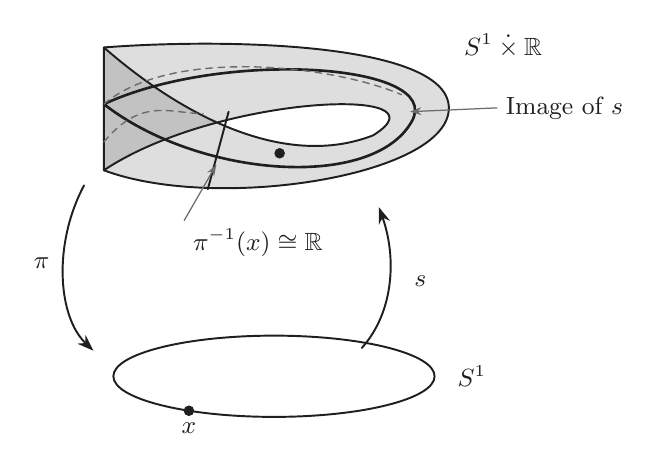
\begin{tikzpicture}[field/diagram, scale=1.20]
    \def\RibbonBoundary{
        (-1.8,2.8)
        .. controls (-0.5,2.9) and (1.8,2.85) .. (1.85,2.18)
        .. controls (1.9,1.45) and (-0.6,1.05) .. (-1.8,1.5) -- cycle
    }
    \fill[FieldRegion] \RibbonBoundary;
    \fill[white] (-0.60176,2.00532) .. controls (-0.05658,1.75905) and (0.52005,1.66360) .. (1.05000,1.87000)
         .. controls (1.66444,2.25312) and (0.52838,2.30704) .. (-0.60176,2.00532) -- cycle;
    \fill[FieldEmphasis] (-1.80000,2.80000) .. controls (-1.44627,2.49049) and (-1.03389,2.20053) .. (-0.60176,2.00532)
         .. controls (-1.03504,1.88965) and (-1.46744,1.72171) .. (-1.80000,1.50000) -- cycle;
    \draw[field/boundary] \RibbonBoundary;
    \draw[field/boundary]
        (-1.8,2.8)
        .. controls (-1,2.1) and (0.1,1.5) .. (1.05,1.87)
        .. controls (1.9,2.4) and (-0.6,2.3) .. (-1.8,1.5);
    \draw[field/curve]
        (-1.8,2.2)
        .. controls (-0.8,1.42) and (1.05,1.28) .. (1.46,2.02)
        .. controls (1.8,2.64) and (-0.55,2.78) .. (-1.8,2.2);
    \draw[field/hidden]
        (-1.8,2.2) .. controls (-1.1,2.8) and (0.6,2.62) .. (1.35,2.3);
    \draw[field/hidden]
        (-1.8,1.8) .. controls (-1.4,2.28) and (-1.1,2.1) .. (-0.75,2.1);
    \draw[field/boundary] (-0.7,1.3) -- (-0.48,2.12);
    \node[field/point] at (0.06,1.68) {};
    \node[anchor=west] at (1.92,2.82) {$S^1\mathbin{\dot\times}\mathbb R$};
    \node[anchor=west] (Image) at (2.36,2.16) {Image of $s$};
    \draw[field/leader] (Image.west) -- (1.44,2.12);
    \node (Fibre) at (-0.17,0.73) {$\pi^{-1}(x)\cong\mathbb R$};
    \draw[field/leader] (Fibre.north west) -- (-0.61,1.56);
    \draw[field/map] (-2.01,1.34)
        .. controls (-2.34,0.72) and (-2.29,-0.05) .. (-1.91,-0.41);
    \node at (-2.46,0.52) {$\pi$};
    \draw[field/map] (0.93,-0.38)
        .. controls (1.27,0.0) and (1.30,0.58) .. (1.11,1.11);
    \node at (1.55,0.33) {$s$};
    \draw[field/boundary] (0,-0.68) ellipse (1.7 and 0.43);
    \node[field/point] at (-0.90,-1.045) {};
    \node[below] at (-0.90,-1.08) {$x$};
    \node[right] at (1.85,-0.68) {$S^1$};
\end{tikzpicture}

        \FieldCaption{I}{1}{}
    \end{minipage}
\end{center}
We observe that every continuous section of $S^1\mathbin{\dot\times}\mathbb R$ is zero at at least one point in sharp contrast to what happens for sections of $S^1\times\mathbb R$. Thus although \emph{locally}, twisted and untwisted functions on $S^1$ possess the same properties, their global behaviour may be rather different.

We shall now give an alternative description of vector bundles in terms of \emph{transition functions}. We follow the notation of Definition~\ref{definition:1.5.1}. For each $i\in I$, $x\in U_i$, we let
\[ \theta_{ix}:E_x\longrightarrow\mathbb R^n \]
denote the restriction of $\theta_i$ to $E_x$ composed with the projection on $\mathbb R^n$.

Define
\[ \theta_{ij}:U_{ij}\longrightarrow\operatorname{GL}(\mathbb R^n) \]
% Original book page 26
by $\theta_{ij}(x)=\theta_{ix}\theta_{jx}^{-1}$, $x\in U_{ij}$, $i,j\in I$ ($\operatorname{GL}(\mathbb R^n)$ denotes the group of linear isomorphisms of $\mathbb R^n$ which is commonly given the alternative notation $\operatorname{GL}(n,\mathbb R)$).

It may easily be verified that the $\theta_{ij}$ are continuous maps which satisfy the cocycle conditions\IndexMark{idx-091}{cocycle condition@Cocycle condition}
\begin{equation}
\left.\begin{aligned}\theta_{ij}&=\theta_{ji}^{-1}\\ \theta_{ij}\cdot\theta_{jk}&=\theta_{ik}\end{aligned}\right\}\tag{A}\label{eq:1:a:2}
\end{equation}
(Inversion and multiplication are in $\operatorname{GL}(\mathbb R^n)$). The $\theta_{ij}$ are called \emph{transition functions}\IndexMark{idx-615}{transition function@Transition function} of the vector bundle $E$. Suppose $s$ is a section of $E$ and $S_i:U_i\to\mathbb R^n$ is the local representation of $s$ on $U_i$ as described above. Then for all $i,j$
\begin{equation} \theta_{ij}S_j=S_i\quad\text{on }U_{ij}.\tag{B}\label{eq:1:b:1}\end{equation}
Conversely, any set of functions $S_i:U_i\to\mathbb R^n$ satisfying B defines a unique section of $E$.

If $E$ and $F$ are vector bundles over $X$ we shall say that a continuous map $A:E\to F$ is a \emph{vector bundle map}\IndexMark{idx-639}{vector bundle@Vector bundle!map@map} if for all $x\in X$, $A(E_x)\subset F_x$ and $A|E_x$ is linear. If $A$ is bijective and $A^{-1}$ is a vector bundle map we shall say that $A$ is a \emph{vector bundle isomorphism}\IndexMark{idx-638}{vector bundle@Vector bundle!isomorphism@isomorphism} and that $E$ and $F$ are \emph{isomorphic vector bundles}.

Suppose that $E,F$ have trivialising maps $\theta_i,\eta_i$ respectively, relative to some (common) cover $\{U_i:i\in I\}$ of $X$. Then for each $i\in I$, $A$ induces a continuous map $A_i:U_i\times\mathbb R^n\to U_i\times\mathbb R^n$ given by $A_i=\eta_i A\theta_i^{-1}$. In turn, $A_i$ induces a continuous map
\[ a_i:U_i\longrightarrow L(\mathbb R^n,\mathbb R^n) \]
such that for all $i,j$
\[ \eta_{ij}a_j=a_i\theta_{ij}\quad\text{on }U_{ij}. \]
% Original book page 27
Conversely, a family of continuous maps $a_i:U_i\to L(\mathbb R^n,\mathbb R^m)$ determines a vector bundle map from $E$ to $F$ provided that for all $i,j$
\begin{equation}\eta_{ij}a_j=a_i\theta_{ij}\quad\text{on }U_{ij}.\tag{C}\label{eq:1:c:1}\end{equation}
Notice that $E$ will be a trivial vector bundle (that is, isomorphic to a trivial vector bundle) if and only if there exist $a_i:U_i\to\operatorname{GL}(\mathbb R^n)$ such that for all $i,j$
\[ a_j=a_i\theta_{ij}\quad\text{on }U_{ij}. \]
Suppose that $\{U_i:i\in I\}$ is an open cover of the topological space $X$ and that we are given continuous maps $\theta_{ij}:U_{ij}\to\operatorname{GL}(\mathbb R^n)$ satisfying the cocycle condition A. Then the $\theta_{ij}$ determine a unique---up to isomorphism---$n$-dimensional real vector bundle over $X$ whose transition functions are the $\theta_{ij}$. To see this we let $Z$ denote the disjoint union over $I$ of the products $U_i\times\mathbb R^n$. We define an equivalence relation on $Z$ by $(i,x,U)\sim(j,y,V)$ iff $x=y$ and $U=\theta_{ij}(x)V$. It is an easy matter to show that $Z/{\sim}$ has the structure of an $n$-dimensional real vector bundle over $X$ with transition functions $\theta_{ij}$ and we leave details to the reader. In the sequel we usually construct vector bundles by specifying a set of transition functions. From C above, it follows that two sets $\theta_{ij},\eta_{ij}:U_{ij}\to\operatorname{GL}(\mathbb R^n)$ of transition functions define isomorphic vector bundles if and only if there exist $a_i:U_i\to\operatorname{GL}(\mathbb R^n)$ such that for all $i,j$, $\eta_{ij}a_j=a_i\theta_{ij}$ on $U_{ij}$.

\paragraph*{Notation.} Let $\mathbb R^{m\prime}$ denote the real dual\IndexMark{idx-636}{vector bundle@Vector bundle!dual@dual} of $\mathbb R^m$. If $A\in L(\mathbb R^m,\mathbb R^n)$, then the \emph{transpose} of\IndexMark{idx-616}{transpose of linear map@Transpose (of linear map)} $A$, $A'$, is the linear map from $\mathbb R^{n\prime}\to\mathbb R^{m\prime}$ characterised by $A'(\phi)(e)=\phi(A(e))$, $\phi\in\mathbb R^{n\prime}$, $e\in\mathbb R^m$.

\paragraph*{Example 4.} Let $E$ be an $n$-dimensional real vector bundle with transition functions $\theta_{ij}$. We define $\theta_{ij}':U_{ij}\to\operatorname{GL}(\mathbb R^{n\prime})$ by
\[ \theta_{ij}'(x)=[\theta_{ij}(x)']^{-1},\quad x\in U_{ij}. \]
The $\theta_{ij}'$ satisfy the cocycle condition A and so are the transition functions for a vector bundle which we call the \emph{dual} vector bundle of $E$ and denote by $E'$. We remark that the trivialisations $\theta_i'$ of $E'$ map naturally to $U_i\times\mathbb R^{n\prime}$ (rather than $U_i\times\mathbb R^n$).
% Original book page 28

Motivated by the previous example, we shall now extend the possible ``fibre models'' of real vector bundles\IndexMark{idx-642}{vector bundles@Vector bundles!exterior product@exterior product}\IndexMark{idx-643}{vector bundles@Vector bundles!symmetric product@symmetric product} to include any finite combination of direct sum, tensor product\IndexMark{idx-644}{vector bundles@Vector bundles!tensor product@tensor product}, exterior and symmetric power of $\mathbb R^n$ and $\mathbb R^{n\prime}$. All these vector space operations extend immediately to vector bundles over a fixed base space $X$. We give one example to illustrate the method and refer the reader to the references for more details. Suppose that $E$ and $F$ are vector bundles over $X$ with transition functions $\theta_{ij}:U_{ij}\to\operatorname{GL}(\mathbb R^m)$ and $\eta_{ij}:U_{ij}\to\operatorname{GL}(\mathbb R^n)$ respectively. $\bigwedge^r F\otimes(E\oplus(\bigodot^s F'))$ will then denote the vector bundle\IndexMark{idx-634}{vector bundle@Vector bundle!complex@complex} over $X$ with fibre model $\bigwedge^r\mathbb R^n\otimes(\mathbb R^m\oplus(\bigodot^r\mathbb R^{n\prime}))$ and transition functions $\psi_{ij}:U_{ij}\to\operatorname{GL}(\bigwedge^r\mathbb R^n\otimes(\mathbb R^m\oplus(\bigodot^r\mathbb R^{n\prime})))$ defined by
\[ \psi_{ij}(x)=(\bigwedge^r\eta_{ij}(x))\otimes(\theta_{ij}(x)\oplus(\bigodot^s\eta_{ij}'(x))),\quad x\in U_{ij}. \]
($\bigwedge^r$ and $\bigodot^s$ denote the operations of $p$th. exterior and $s$th. symmetric power respectively).
% The inconsistent r,s,p in this paragraph are present in the source.

Suppose that $X$ is a differential manifold (with $C^\infty$ structure). We can define smooth (that is $C^\infty$) real vector bundles over $X$ in the obvious way and everything we have said above generalises immediately to the smooth case. If $E$ is a smooth vector bundle over $X$, we let $C^r(E)$ denote the vector space of $C^r$ sections of $E$, $1\leq r\leq\infty$.

\paragraph*{Example 5.} Let $M$ be an $m$-dimensional differential manifold with smooth atlas $\{(U_i,\phi_i):i\in I\}$. We define $C^\infty$ maps $\phi_{ij}:U_{ij}\to\operatorname{GL}(\mathbb R^m)$ by $\phi_{ij}(x)=D(\phi_i\phi_j^{-1})(\phi_j(x))$. The $\phi_{ij}$ are the transition functions for the (real) \emph{tangent bundle}\IndexMark{idx-598}{tangent bundle@Tangent bundle!real@real} of $M$ which we denote in the sequel by $\mathcal T M$. The (real) \emph{cotangent bundle}\IndexMark{idx-140}{cotangent bundle@Cotangent bundle} of $M$, $\mathcal T'M$, is the dual bundle of $\mathcal T M$ with transition functions $\phi_{ij}'$ (See Abraham and Marsden \cite{bib:I:abraham-r-and-marsden-j-e:1}, Chillingworth \cite{bib:I:chillingworth-d-r-j:1} and Lang \cite{bib:I:lang-s:1} for more details).

We now turn our attention to vector bundles with fibre a complex vector space. An \emph{$m$-dimensional complex vector bundle} $E$ over $X$ is defined exactly as in Definition~\ref{definition:1.5.1} except that ``real'' and ``$\mathbb R^n$'' are everywhere replaced by ``complex'' and ``$\mathbb C^m$'' respectively. We leave the writing out of the formal definitions of complex vector bundles, sections, transition functions, etc. to the reader. Sections of an $m$-dimensional complex vector bundle will locally be $\mathbb C^m$-valued functions: globally they may be twisted.
% Original book page 29

One important feature of complex vector bundles is the greater complexity of the fibre models which involve not only duals but also conjugates. But first we need to review some complex linear algebra.

If $J:\mathbb C^m\to\mathbb C^m$ denotes scalar multiplication by $i$, then $J$ is a $\mathbb C$-linear isomorphism of $\mathbb C^m$ satisfying $J^2=-I$. The usual complex structure\IndexMark{idx-111}{complex structure@Complex structure!on vector space@on vector space}\IndexMark{idx-113}{complex structure@Complex structure!conjugate structure@conjugate structure} on $\mathbb C^m$ may be defined in terms of $J$ and the underlying real structure on $\mathbb C^m$ by
\[ (a+ib)Z=aZ+bJ(Z),\quad a,b\in\mathbb R,\quad Z\in\mathbb C^m. \]
The \emph{conjugate complex structure}\IndexMark{idx-125}{conjugate@Conjugate!vector space@vector space} on $\mathbb C^m$ is defined by
\[ (a+ib)Z=aZ-bJ(Z),\quad a,b\in\mathbb R,\quad Z\in\mathbb C^m. \]
We denote the resulting complex vector space by $\overline{\mathbb C}^{m}$. Suppose $A\in L(\mathbb C^m,\mathbb C^n)$, we define $\overline A\in L(\overline{\mathbb C}^{m},\overline{\mathbb C}^{n})$ by simply requiring that $A=\overline A$ on the common underlying set of $\mathbb C^m$ and $\overline{\mathbb C}^{m}$ (We should emphasise that all linear maps here are assumed \emph{complex} linear unless the contrary is explicitly stated).

We let $\mathbb C^{m*}=L(\mathbb C^m,\mathbb C)$ denote the \emph{conjugate dual space}\IndexMark{idx-127}{conjugate@Conjugate!dual space@dual space} of $\mathbb C^m$. If $A\in L(\mathbb C^m,\mathbb C^n)$, we define the \emph{transpose}\IndexMark{idx-617}{transpose of linear map@Transpose (of linear map)} $A^*\in L(\mathbb C^{n*},\mathbb C^{m*})$ exactly as in the real case.
% "conjugate dual space" here is the wording of the source.

We let $\overline{\mathbb C}^{m*}$ denote the complex vector space of conjugate complex linear maps on $\mathbb C^m$. We call $\overline{\mathbb C}^{m*}$ the \emph{conjugate dual space} of $\mathbb C^m$. Note that $f\in\overline{\mathbb C}^{m*}$ if $f:\mathbb C^m\to\mathbb C$ is $\mathbb R$-linear and $f(\lambda Z)=\overline\lambda f(Z)$, $\lambda\in\mathbb C$, $Z\in\mathbb C^m$. Clearly, $\overline{\mathbb C}^{m*}\cong L(\overline{\mathbb C}^{m},\mathbb C)$. Moreover, $\overline{\mathbb C^{m*}}\cong\overline{\mathbb C}^{m*}$ where we map $\phi\in\mathbb C^{m*}$ to $\overline\phi\in\overline{\mathbb C}^{m*}$ and $\overline\phi(e)=\overline{\phi(e)}$, $e\in\mathbb C^m$. If $A\in L(\mathbb C^m,\mathbb C^n)$, we define the \emph{conjugate transpose} $\overline A^*\in L(\overline{\mathbb C}^{n*},\overline{\mathbb C}^{m*})$ by
\[ \overline A^*(\phi)(e)=\phi(A(e)),\quad e\in\mathbb C^m,\quad\phi\in\overline{\mathbb C}^{n*}. \]
Finally, if $A\in L(\mathbb C^m,\mathbb C^n)$ has matrix $[a_{ij}]$ relative to the standard bases of $\mathbb C^m$ and $\mathbb C^n$, the reader may easily verify that the matrices of $\overline A$, $A^*$ and $\overline A^*$ are respectively $[\overline{a_{ij}}]$, $[a_{ji}]$ and $[\overline{a_{ji}}]$ relative to the naturally induced bases on $\overline{\mathbb C}^m,\ldots,\overline{\mathbb C}^{n*}$.
% Original book page 30
\paragraph*{Example 6.} Let $E$ be a complex vector bundle with transition functions $\theta_{ij}:U_{ij}\to\operatorname{GL}(\mathbb C^m)$. We define maps
\begin{align*}
\overline\theta_{ij}:U_{ij}&\longrightarrow\operatorname{GL}(\overline{\mathbb C}^m),\\
\theta_{ij}^*:U_{ij}&\longrightarrow\operatorname{GL}(\mathbb C^{m*}),\\
\overline\theta_{ij}^*:U_{ij}&\longrightarrow\operatorname{GL}(\overline{\mathbb C}^{m*})
\end{align*}
by $\overline\theta_{ij}(x)=\overline{\theta_{ij}(x)}$, $\theta_{ij}^*(x)=[\theta_{ij}(x)^*]^{-1}$, $\overline\theta_{ij}^*(x)=[\overline{\theta_{ij}(x)}^*]^{-1}$, $x\in U_{ij}$.

Now $\overline\theta_{ij}$, $\theta_{ij}^*$, $\overline\theta_{ij}^*$ satisfy the cocycle condition A and so are the transition functions for complex vector bundles which we call the \emph{conjugate} bundle, $\overline E$, \emph{dual} bundle, $E^*$, and \emph{conjugate dual}\IndexMark{idx-635}{vector bundle@Vector bundle!conjugate dual@conjugate (dual)} bundle, $\overline E^*$, of $E$ respectively.

Exactly as for the real case we may now extend the possible fibre models of complex vector bundles to include finite combinations of direct sum, tensor product, exterior and symmetric powers of $\mathbb C^m$ and its conjugate and dual spaces. All these operations extend immediately to complex vector bundles over a fixed base space and we leave formal details to the reader.

\paragraph*{Remarks.}
\begin{enumerate}
\item We shall show in Chapter 9 that, as complex vector bundles, $E$ is isomorphic to $\overline E^*$ and $E^*$ is isomorphic to $\overline E$. However, these isomorphisms are not natural and in the sequel it will often be convenient to regard these bundles as all being distinct.
\item If $E$ is a 1-dimensional complex vector bundle, we shall usually refer to $E$ as a \emph{complex line bundle}\IndexMark{idx-104}{complex line bundle@Complex line bundle}\IndexMark{idx-373}{line bundle@Line bundle!complex@complex}. Since $\operatorname{GL}(\mathbb C)\cong\mathbb C^\bullet$, the transition functions for a complex line bundle may be equivalently given by non-vanishing complex valued functions: $\theta_{ij}:U_{ij}\to\mathbb C^\bullet$.
\end{enumerate}
\paragraph*{Examples.}
\paragraph*{7.} Let $\operatorname{CLB}(X)$ denote the set of isomorphism classes of complex line bundles over $X$. We claim that $\operatorname{CLB}(X)$ has the natural structure of an abelian group with identity the trivial bundle $\underline{\mathbb C}$ and product and inversion respectively defined by

% Original book page 31
\begin{align*}
E\cdot F&=E\otimes F,\quad E,F\in\operatorname{CLB}(X),\\
E^{-1}&=E^*,\quad E\in\operatorname{CLB}(X).
\end{align*}
Certainly $E\cdot\underline{\mathbb C}=\underline{\mathbb C}\cdot E=E$ for all $E\in\operatorname{CLB}(X)$. We verify that $E^*$ is the inverse of $E$ with respect to $\otimes$ and leave the remaining details to the reader. To verify that $E^*$ is the inverse of $E$ it is enough to note that there is a natural isomorphism $E\otimes E^*\cong\underline{\mathbb C}$ induced from the dual pairing $E_x\otimes E_x^*\cong\mathbb C$, $x\in X$ (Perhaps we should remark that for the group $\operatorname{RLB}(X)$ of \emph{real} line bundles\IndexMark{idx-375}{line bundle@Line bundle!real@real} on $X$, $L$ is isomorphic to $L'$, $L\in\operatorname{RLB}(X)$, and so $L^2\cong\underline{\mathbb R}$, for all $L\in\operatorname{RLB}(X)$).

\paragraph*{2.} Let $M$ be a Riemann surface with complex analytic atlas $\{(U_i,\phi_i):i\in I\}$. We define $\phi_{ij}:U_{ij}\to\operatorname{GL}(\mathbb C)$ by $\phi_{ij}(z)=\partial(\phi_i\phi_j^{-1})/\partial z(\phi_j(z))$, $z\in U_{ij}$. The $\phi_{ij}$ are complex analytic maps and are the transition functions for the \emph{holomorphic tangent bundle}\IndexMark{idx-599}{tangent bundle@Tangent bundle!holomorphic@holomorphic}\IndexMark{idx-601}{tangent bundle@Tangent bundle!anti holomorphic@anti-holomorphic} of $M$ which we denote in the sequel by $TM$.
% The source numbers this example 2, between examples 7 and 9.

$\phi_{ij}^*:U_{ij}\to\operatorname{GL}(\mathbb C^*)$ are also analytic maps and define the transition functions for the \emph{holomorphic cotangent bundle}\IndexMark{idx-142}{cotangent bundle@Cotangent bundle!holomorphic anti holomorphic@holomorphic, anti-holomorphic}, $TM^*$, of $M$.

$\overline\phi_{ij}:U_{ij}\to\operatorname{GL}(\overline{\mathbb C})$ are $C^\infty$ maps (not analytic!) and are the transition functions for the \emph{anti-holomorphic tangent bundle}, $\overline{TM}$, of $M$.

$\overline\phi_{ij}^*:U_{ij}\to\operatorname{GL}(\overline{\mathbb C}^*)$ are $C^\infty$ maps and are the transition functions for the \emph{anti-holomorphic cotangent bundle}, $\overline{TM}^*$, of $M$.

We shall now show how the operator $\partial/\partial\bar z$ extends to a Riemann surface $M$ as a map $\bar\partial:C^\infty(M)\to C^\infty(\overline{TM}^*)$. First we need to note the composite mapping formula\IndexMark{idx-123}{composite mapping formula@Composite mapping formula} for $\partial/\partial z$, $\partial/\partial\bar z$:

Suppose $h$ and $g$ are $C^1$ complex valued functions defined on open subsets of $\mathbb C$. Then
\begin{align}
\partial(gh)/\partial z&=(\partial g/\partial z)(\partial h/\partial z)+(\partial g/\partial\bar z)\overline{\partial h/\partial\bar z},\tag{*}\label{eq:1:star:1}\\
\partial(gh)/\partial\bar z&=(\partial g/\partial z)(\partial h/\partial\bar z)+(\partial g/\partial\bar z)\overline{\partial h/\partial z}.\tag{**}\label{eq:1:star:2}
\end{align}
The proof is most easily done by taking real and imaginary parts and applying the chain rule for $\partial/\partial x$ and $\partial/\partial y$.
% Original book page 32

Let $(U_i,\phi_i)$, $(U_j,\phi_j)$ be charts for $M$ and $f\in C^\infty(M)$. Then
\begin{align*}
\partial(f\phi_i^{-1})/\partial\bar z
&=\partial(f\phi_j^{-1}\phi_j\phi_i^{-1})/\partial\bar z\\
&=\partial(f\phi_j^{-1})/\partial\bar z\ \overline{\partial(\phi_j\phi_i^{-1})/\partial z},\quad\text{using ** above}\\
&=\overline\phi_{ij}^*\ \partial(f\phi_j^{-1})/\partial\bar z,
\end{align*}
where $\overline\phi_{ij}^*$ are the transition functions for $\overline{TM}^*$. Hence $\partial(f\phi_i^{-1})/\partial\bar z$ are the local representatives of a $C^\infty$ section of $\overline{TM}^*$ which in the sequel we shall denote by $\bar\partial f$. The operator $\bar\partial:C^\infty(M)\to C^\infty(\overline{TM}^*)$ clearly has kernel equal to $A(M)$. We shall return to the question of how far $\bar\partial$ fails to be surjective at the end of this section.

The fibre model for $\overline{TM}^*$ is $\overline{\mathbb C}^*$ and we denote the standard basis of $\overline{\mathbb C}^*$ by $d\bar z$. Suppose that $g\in C^\infty(\overline{TM}^*)$, then the local representative of $g$ with respect to a chart $(U_i,\phi_i)$ is given by $g_i\,d\bar z$, where $g_i=\overline\phi_i^*g\in C^\infty(U_i)$. If $f\in C^\infty(M)$, the local representative of $\bar\partial f$ is $\partial f_i/\partial\bar z\,d\bar z$, where $f_i=f\phi_i^{-1}\in C^\infty(U_i)$.

We may similarly define $\partial:C^\infty(M)\to C^\infty(TM)$ and the local representative of $\partial f$ with respect to a chart $(U_i,\phi_i)$ will be $\partial f_i/\partial z\,dz$, where $dz$ denotes the standard basis of $\mathbb C^*$.
% Source prints TM rather than TM* in the preceding codomain.

We remark that $df=\partial f+\bar\partial f$ as is easily verified by the local computation $\partial f/\partial z\,dz+\partial f/\partial\bar z\,d\bar z=\partial f/\partial x\,dx+\partial f/\partial y\,dy$.

\FieldHeading{Definition}{1.5.3}{}\FieldTarget{definition:1.5.3}{1.5.3} Let $\theta_{ij}:U_{ij}\to\operatorname{GL}(\mathbb C)$ be the transition functions for a complex line bundle\IndexMark{idx-374}{line bundle@Line bundle!holomorphic@holomorphic} $E$ over the Riemann surface $M$. If the $\theta_{ij}$ are all analytic, we shall say that $E$ is a \emph{holomorphic line bundle}\IndexMark{idx-294}{holomorphic line bundle@Holomorphic line bundle} over $M$.

\paragraph*{Examples.}
\paragraph*{9.} If $M$ is a Riemann surface, $TM$ and $TM^*$ are holomorphic line bundles over $M$.

\paragraph*{10.} Let $\operatorname{HLB}(M)$ denote the set of isomorphism classes of holomorphic line bundles over the Riemann surface $M$ (isomorphism here is, of course, analytic line bundle isomorphism, and may be given explicitly in terms of analytic functions using condition C above).
% Original book page 33

As in the previous example on $\operatorname{CLB}(M)$, $\operatorname{HLB}(M)$ has the natural structure of an abelian group with composition defined as tensor product and inverse as dual (see also below).

Holomorphic line bundles and their generalisation, holomorphic vector bundles, will be of the greatest importance in the sequel. As we shall see they provide a particularly potent geometric framework for many problems in complex analysis.

Suppose that $E$ is a holomorphic line bundle on the Riemann surface $M$ with transition functions $\theta_{ij}$ relative to the cover $\{U_i\}$. A family $S_i\in A(U_i)$ will define an \emph{analytic section} of $E$ if, for all $i,j$,
\[ S_i=\theta_{ij}S_j\quad\text{on }U_{ij}. \]
A family $M_i\in M(U_i)$ will define a \emph{meromorphic section}\IndexMark{idx-393}{meromorphic section@Meromorphic section!of vector bundle@of vector bundle} $m$ of $E$ if, for all $i,j$,
\[ M_i=\theta_{ij}M_j\quad\text{on }U_{ij}. \]
We denote the sets of analytic and meromorphic sections of $E$ by $\Omega(E)$ and $M(E)$ respectively. We let $M^*(E)$ denote the set of non-zero meromorphic sections of $E$. As in \S\S3,4, we define $\operatorname{ord}(m,z)$\IndexMark{idx-424}{order of pole zero@Order (of pole, zero)}, $m\in M(E)$, $z\in M$; $\operatorname{div}(m)$, $m\in M^*(E)$ and, if $M$ is compact, $\deg(\operatorname{div}(m))$, $m\in M^*(E)$.

With the above formalism out of the way we can now rapidly achieve one of the primary goals of this section: The geometric formulation of the problem of generalising Weierstrass' theorem to compact Riemann surfaces.

For the remainder of this section we shall assume that $M$ is a compact Riemann surface.

\FieldHeading{Proposition}{1.5.4}{}\FieldTarget{proposition:1.5.4}{1.5.4}\IndexMark{idx-185}{divisor class map@Divisor class map} There is a natural homomorphism $[\ ]:\mathcal D(M)\to\operatorname{HLB}(M)$ satisfying the property that for any $d\in\mathcal D(M)$ there exists $s(d)\in M^*([d])$ such that $\operatorname{div}(s(d))=d$. Furthermore, $s(d)$ is determined uniquely up to multiplication by elements of $\mathbb C^\bullet$.
\begin{proof}
As we showed in \hyperref[sec:1:3]{\S3}, any divisor may be uniquely specified by an open cover $\{U_i\}$ of $M$ and $m_i\in M^*(U_i)$ such that, for all $i,j$, $m_i/m_j\in A^*(U_{ij})$. Define $\theta_{ij}=m_i/m_j\in A^*(U_{ij})$. Clearly the $\theta_{ij}$ are
% Original book page 34
the transition functions for a holomorphic line bundle on $M$ which we denote by $[d]$. We leave it to the reader to verify that $d\mapsto[d]$ is a group homomorphism.

We define $s(d)_i=m_i\in M^*(U_i)$ and observe that $\theta_{ij}s(d)_j=s(d)_i$ on $U_{ij}$. Hence the $s(d)_i$ are the local representatives of a meromorphic section $s(d)$ of $[d]$. Obviously $\operatorname{div}(s(d))=d$. We leave the remaining assertions as an exercise---see also Lemma~\ref{lemma:1.5.6}.
\end{proof}
\paragraph*{Remark.} Proposition~\ref{proposition:1.5.4} gives a ``formal'' solution to the problem of which divisors are divisors of meromorphic functions: Every divisor is the divisor of a ``twisted'' meromorphic function.

\FieldHeading{Proposition}{1.5.5}{}\FieldTarget{proposition:1.5.5}{1.5.5} A divisor $d$ on $M$ is the divisor of a meromorphic function if and only if $[d]$ is trivial as a holomorphic line bundle.
\begin{proof}
Suppose $d=\operatorname{div}(m)$, $m\in M^*(M)$. Let $\{U_i\}$ be any open cover of $M$. Set $m_i=m|U_i$ and $\theta_{ij}=m_i/m_j=1$. The $m_i$ then define the divisor $d$ and, since $\theta_{ij}=1$, $[d]$ is holomorphically trivial. Conversely, if $[d]$ is holomorphically trivial, there exists a nowhere zero analytic section $s$ of $[d]$. In terms of local representatives $s_i\in A^*(U_i)$ we must have $\theta_{ij}s_i=s_j$, where $\theta_{ij}$ are the transition functions of $[d]$. But $\theta_{ij}=m_i/m_j$, where the $m_i$ define the divisor $d$. Therefore, we have $m_i/s_i=m_j/s_j$ on $U_{ij}$ and we may define $m\in M^*(M)$ by $m|U_i=m_i/s_i$. Obviously, $\operatorname{div}(m)=d$.
% Source prints theta_ij s_i = s_j; indices retained.
\end{proof}
\FieldHeading{Lemma}{1.5.6}{}\FieldTarget{lemma:1.5.6}{1.5.6} Suppose that $L\in\operatorname{HLB}(M)$ and $s,t\in M^*(L)$. Then $s/t$ naturally defines a non-zero meromorphic function on $M$.
\begin{proof}
Suppose that $L$ has transition functions $\theta_{ij}$ relative to some open cover $\{U_i\}$ of $M$. Then, $s,t$ are locally given by $s_i,t_i\in M^*(U_i)$ subject to the relations $\theta_{ij}s_{ij}=s_i$, $\theta_{ij}t_j=t_i$ for all $i,j$. Therefore, $s_j/t_j=s_i/t_i$ on $U_{ij}$ and so we may define $m\in M^*(M)$ by $m|U_i=s_i/t_i$.
% Source prints s_ij in the first relation; retained.
\end{proof}
\paragraph*{Remark.} Notice that $t^{-1}$ naturally defines a meromorphic section of $L^{-1}=L^*$ and so $s/t$ may equivalently be defined by using the pairing $M^*(L)\times M^*(L^{-1})\to M^*(M)$ induced from the dual pairing $L\otimes L^*\cong\underline{\mathbb C}$.
% Original book page 35

\FieldHeading{Proposition}{1.5.7}{}\FieldTarget{proposition:1.5.7}{1.5.7} Let $L\in\operatorname{HLB}(M)$ and suppose $M^*(L)\ne\varnothing$. Given $s\in M^*(L)$, set $\deg(s)=\deg(\operatorname{div}(s))$. Then $\deg(s)$ is independent of $s$ and depends only on $L$.
\begin{proof}
Let $s,t\in M^*(L)$. Clearly, $\operatorname{div}(s/t)=\operatorname{div}(s)-\operatorname{div}(t)$. But $s/t\in M^*(M)$ and so by Lemma~\ref{lemma:1.4.3}, $\deg(s/t)=0$. Hence $\deg(s)=\deg(t)$.
\end{proof}
For every holomorphic line bundle $L$ on $M$ that admits a non-trivial meromorphic section we may define the \emph{degree of $L$}, $\deg(L)$, to be $\deg(s)$, where $s$ is any non-trivial meromorphic section of $L$. Notice that if $\deg(L)\ne0$, then $L$ cannot be holomorphically trivial. It is also clear that if $d\in\mathcal D(M)$ then $\deg(d)=\deg([d])$.

The degree of $L$ is an important topological invariant of $L$. In fact we shall show later (Example 14, \hyperref[sec:6:3]{\S3, Chapter 6}) that $\deg(L)=0$ if and only if $L$ is trivial as a \emph{complex} line bundle.

What we have achieved above is to shift the problem of determining which divisors are divisors of meromorphic functions to the apparently more general problem of determining which holomorphic line bundles admit non-trivial meromorphic sections. We already know that a divisor $d$ can be the divisor of a meromorphic function on $M$ only if $\deg([d])=\deg(d)=0$. Let $\operatorname{HLB}_0(M)$ denote the subgroup of $\operatorname{HLB}(M)$ consisting of line bundles of degree zero. Two problems naturally arise at this stage.
\begin{enumerate}
\item Show that $[\ ]:\mathcal D(M)\to\operatorname{HLB}(M)$ is onto.
\item Describe $\operatorname{HLB}_0(M)$.
\end{enumerate}
To show that $[\ ]$ is onto amounts to proving that every holomorphic line bundle on $M$ has a non-trivial meromorphic section. The existence of such meromorphic sections follows from a rather general finiteness theorem that we prove in Chapter~\ref{ch:7} (see the exercises at the end of \hyperref[sec:7:5]{\S5, Chapter 7}). Once we know that $[\ ]$ is onto it is an easy matter to prove Riemann's part\IndexMark{idx-529}{riemann s inequality@Riemann's inequality} of the \emph{Riemann--Roch} theorem\IndexMark{idx-527}{riemann roch theorem@Riemann--Roch theorem}:

For any divisor $d$ on $M$ we have
\[ \dim_{\mathbb C}\Omega([d])\geq\deg(d)+1-g, \]
% Original book page 36
where $g$ denotes the genus of $M$.

This result is already sufficient to prove useful existence theorems for meromorphic functions on compact Riemann surfaces. The full Riemann--Roch theorem depends on Serre-duality which we establish in Chapter 10 (see also \hyperref[sec:7:5]{\S5, Chapter 7}).

As far as the second problem goes, $\operatorname{HLB}_0(M)$ may be shown to have the structure of a compact complex Lie group of complex dimension $g$. The group $\operatorname{HLB}_0(M)$ is usually referred to as the \emph{Picard variety}\IndexMark{idx-436}{picard variety@Picard variety} of $M$ and denoted by $\operatorname{Pic}(M)$. Whilst the dimension of $\operatorname{Pic}(M)$ depends only on the genus on $M$ its complex structure depends on the complex structure of $M$. Abel's theorem gives explicit conditions on a divisor in order that it determine the identity of $\operatorname{Pic}(M)$, that is the trivial holomorphic line bundle (We refer to Gunning \cite{bib:I:gunning-r-c:1} for details).

We conclude this section by briefly indicating the role that $\bar\partial$ plays in the study of meromorphic functions on a compact Riemann surface.

Suppose that $E$ is a holomorphic line bundle on $M$ with transition functions $\theta_{ij}$. We shall investigate conditions under which $E$ is holomorphically trivial. First observe that, as in the proof of Theorem~\ref{theorem:1.3.3}, $\{(2\pi i)^{-1}\log\theta_{ij}\}$ defines a class $\gamma_E$ in $H^2(M,\mathbb Z)$. The class $\gamma_E$ will be zero if and only if $E$ is trivial as a complex line bundle. From now on we assume $E$ is complex trivial, that is $E\in\operatorname{Pic}(M)$. We may choose the branches of $\log\theta_{ij}$ so that $\log\theta_{ij}=h_{ij}\in A(U_{ij})$ determine an additive cocycle (see the proof of Theorem~\ref{theorem:1.3.3}). Now $E$ is trivial as a complex line bundle if there exist $g_i\in C^\infty(U_i)$ such that $h_{ij}=g_j-g_i$ (exponentiate!). Define $F\in C^\infty(\overline{TM}^*)$ by $F|U_i=\bar\partial g_i$. We can solve $\bar\partial u=-F$ if the class of $F$ in $C^\infty(\overline{TM}^*)/\bar\partial C^\infty(M)$ is zero. Given such a solution, the functions $a_i=\exp(g_i+u)\in A^*(U_i)$ will then give a holomorphic trivialisation of $E$. The basic result now is that the complex vector space $C^\infty(\overline{TM}^*)/\bar\partial C^\infty(M)$ is finite dimensional (the dimension is actually $g$, the genus of $M$). If we are more careful in our arguments we see that to prove $E$ is holomorphically trivial it is enough to find $u\in C^\infty(M)$ such that $\bar\partial u+F$ exponentiates to zero. Further analysis then shows that $H^1(M,\mathbb Z)$ ($\cong\mathbb Z^{2g}$) determines an integer lattice in $C^\infty(\overline{TM}^*)/\bar\partial C^\infty(M)$ and that a necessary and sufficient condition for $E$ to be holomorphically trivial is that $F$ determines a lattice point. The Picard variety is then isomorphic to the torus $(C^\infty(\overline{TM}^*)/\bar\partial C^\infty(M))/H^1(M,\mathbb Z)$. We
% Original book page 37
refer to Gunning \cite{bib:I:gunning-r-c:1} for details. In Chapter~\ref{ch:7} we shall show that $C^\infty(\overline{TM}^*)/\bar\partial C^\infty(M)$ is finite dimensional using rather general arguments about sheaves. In Chapter 10 we give a more direct proof of finiteness and much more explicit description of the quotient $C^\infty(\overline{TM}^*)/\bar\partial C^\infty(M)$ using Hodge theory.

\paragraph*{Exercises.}
\begin{enumerate}
\item Let $f:X\to Y$ be a continuous map between topological spaces and $E$ be a vector bundle on $Y$ with transition functions $\theta_{ij}$ relative to some cover $\{U_i\}$ of $Y$. Show that $\theta_{ij}f$ are transition functions for a vector bundle $f^*E$ over $X$ (the ``pull-back\IndexMark{idx-485}{pull back@Pull-back!of vector bundle@of vector bundle}\IndexMark{idx-486}{pull back@Pull-back!of divisor@of divisor} bundle\IndexMark{idx-640}{vector bundle@Vector bundle!pull back@pull-back} of $E$ by $f$''). Verify that, up to vector bundle isomorphism, $f^*E$ depends only on $E$ and $f$ and not on any choices we have made. Show also that in case $f$ is a holomorphic map between Riemann surfaces our construction determines a homomorphism $f^*:\operatorname{HLB}(Y)\to\operatorname{HLB}(X)$.
\item Let $f:X\to Y$ be a holomorphic map between Riemann surfaces and let $d\in\mathcal D(Y)$. Prove that $f^*[d]\cong[f^*(d)]$ (see Exercise 5, \hyperref[sec:1:4]{\S4}).
\item Let $M$ be a Riemann surface and $d,d'\in\mathcal D(M)$. We say $d$ and $d'$ are \emph{linearly equivalent}\IndexMark{idx-376}{linear equivalence of divisors@Linear equivalence of divisors} if $d-d'=\operatorname{div}(m)$ for some $m\in M^*(M)$. Show that $d$ and $d'$ are linearly equivalent if and only if $[d]\cong[d']$ as holomorphic line bundles.
\item Let $\Omega$ be a domain in $\mathbb C$. Prove that every holomorphic line bundle on $\Omega$ is holomorphically trivial.
\item Let $E,F$ be vector bundles over the differential manifold $M$. Prove that $C^\infty(E'\otimes F)$ is naturally isomorphic to the space of smooth vector bundle maps from $E$ to $F$, $\operatorname{Hom}(E,F)$.
\item Suppose that $E,F$ are vector bundles over the differential manifold $M$ and $\phi:C^\infty(E)\to C^\infty(F)$ is a $C_{\mathbb R}^\infty(M)$-linear map. Prove that $\phi$ is induced from a vector bundle map $\Phi:E\to F$. That is, show that $\phi(s)(x)=\Phi(s(x))$, $x\in M$, $s\in C^\infty(E)$. Deduce that $\phi$ determines a unique section $\gamma$ of $C^\infty(E'\otimes F)$ characterised by $\langle\gamma,X\rangle=\phi(X)$, $X\in C^\infty(E)$, where $\langle\ ,\ \rangle$ is induced from the dual pairing between $E$ and $E'$.
\end{enumerate}

% Original book page 38
\section*{Appendix to Chapter~\ref{ch:1}}\label{app:1}
\addcontentsline{toc}{section}{Appendix to Chapter~\ref{ch:1}}
In the first part of this appendix we prove a number of results related to Cauchy's integral formula\IndexMark{idx-070}{cauchy s integral formula@Cauchy's integral formula} that will be used later in the text as well as in the proof of Theorem~\ref{theorem:1.3.1}. The main element in the proof of Theorem~\ref{theorem:1.3.1} is the Runge approximation theorem and this, together with the proof of Theorem~\ref{theorem:1.3.1}, constitute the remainder of the appendix.

In the statement of the next three results we shall assume that $\Omega$ is a bounded open domain in $\mathbb C$ with $\partial\Omega$ a finite union of piecewise $C^1$ curves. We use the notation $C^1(\overline\Omega)$ to denote the set of functions on $\overline\Omega$ which are restrictions of $C^1$ functions defined on some neighbourhood of $\overline\Omega$.

\FieldHeading{Lemma}{A1.1}{}\FieldTarget{lemma:A1.1}{A1.1} Let $f\in C^1(\overline\Omega)$. Then
\[ \int_{\partial\Omega}f\,dz=\int_\Omega\partial f/\partial\bar z\,d\bar z\,dz=2i\int_\Omega\partial f/\partial\bar z\,dx\,dy. \]
\begin{proof} Stoke's or Green's theorem in the plane (take real and imaginary parts). \end{proof}

\FieldHeading{Theorem}{A1.2}{ (Cauchy's Integral Formula).}\FieldTarget{theorem:A1.2}{A1.2} Let $u\in C^1(\overline\Omega)$. Then
\[ u(\zeta)=(2\pi i)^{-1}\int_{\partial\Omega}\frac{u(z)}{z-\zeta}\,dz+\frac1\pi\int_\Omega\partial u/\partial\bar z\,/(z-\zeta)\,dx\,dy,\quad\zeta\in\Omega. \]
\begin{proof} Let $\Omega_\varepsilon=\{z\in\Omega:|z-\zeta|>\varepsilon\}$, where $\varepsilon<d(\zeta,\partial\Omega)$. Apply Lemma~\ref{lemma:A1.1} with $f(z)=u(z)/(z-\zeta)$ and let $\varepsilon\to0$. \end{proof}

\FieldHeading{Corollary}{A1.3}{}\FieldTarget{corollary:A1.3}{A1.3} Let $u\in C^0(\overline\Omega)$ and suppose $u$ is analytic in $\Omega$. Then
\[ u(\zeta)=(2\pi i)^{-1}\int_{\partial\Omega}\frac{u(z)}{z-\zeta}\,dz,\quad\zeta\in\Omega. \]
\FieldHeading{Corollary}{A1.4}{}\FieldTarget{corollary:A1.4}{A1.4} Let $\Omega$ be a domain in $\mathbb C$ and suppose that $u_n$, $n\geq1$, is a sequence in $A(\Omega)$ which converges uniformly on compact subsets of $\Omega$ to a function $u$ on $\Omega$. Then $u\in A(\Omega)$.
\begin{proof} Apply Corollary~\ref{corollary:A1.3} to $u_n-u_m$ restricted to closed discs contained in $\Omega$ to deduce that $\partial u_n/\partial z$ converges uniformly on compact subsets of $\Omega$. Since $\partial u_n/\partial\bar z=0$, it follows that $u$ is $C^1$ on $\Omega$ with $\partial u/\partial\bar z=0$. \end{proof}
% Original book page 39

\FieldHeading{Corollary}{A1.5}{ (Montel's theorem).}\IndexMark{idx-402}{montel s theorem@Montel's theorem}\FieldTarget{corollary:A1.5}{A1.5} Let $\Omega$ be a domain in $\mathbb C$ and suppose that $u_n$, $n\geq1$, is a sequence in $A(\Omega)$ which is uniformly bounded on every compact subset of $\Omega$. Then there is a subsequence of the $u_n$ which converges uniformly on compact subsets of $\Omega$ to a limit $u\in A(\Omega)$.
\begin{proof} By Cauchy's inequalities (Exercise 2, \hyperref[sec:1:1]{\S1}) the sequence $\partial u_n/\partial z$ is uniformly bounded on any closed disc $D_r(z)\subset\Omega$. Hence $\partial u_n/\partial z$ is uniformly bounded on any compact subset of $\Omega$. Therefore the sequence $u_n$ is an equicontinuous family and, by Ascoli's theorem, has a subsequence converging uniformly on compact subsets of $\Omega$ to a function $u$. By Corollary~\ref{corollary:A1.4}, $u\in A(\Omega)$. \end{proof}

Let $\mu$ be a (finite, complex regular, Borel) measure on $\mathbb C$. The \emph{support} of $\mu$, $\operatorname{supp}(\mu)$, is defined to be the smallest closed subset of $\mathbb C$ outside of which $\mu$ is zero.

\FieldHeading{Theorem}{A1.6}{}\FieldTarget{theorem:A1.6}{A1.6} Let $\mu$ be a measure on $\mathbb C$ with compact support. Then
\[ u(\zeta)=\int_{\mathbb C}(z-\zeta)^{-1}\,d\mu(z) \]
defines an analytic function outside $\operatorname{supp}(\mu)$. If $d\mu=\frac1\pi\phi\,dx\,dy$, $\phi\in C_c^\infty(\mathbb C)$, then $u\in C^\infty(\mathbb C)$ and $\partial u/\partial\bar z=\phi$.
\begin{proof}
Certainly $u$ is $C^1$ outside $\operatorname{supp}(\mu)$---in fact $C^\infty$---and differentiating under the integral sign we see that $\partial u/\partial\bar z=0$. Hence $u$ is analytic outside $\operatorname{supp}(\mu)$. For the second statement we see by changing variables that
\[ u(\zeta)=-\frac1\pi\int_{\mathbb C}\phi(\zeta-z)z^{-1}\,dx\,dy. \]
Now $z^{-1}$ is integrable on compact sets and so $u\in C^\infty(\mathbb C)$. Moreover,
\begin{align*}
\partial u/\partial\bar\zeta&=\frac1\pi\int_{\mathbb C}\partial\phi/\partial\bar\zeta(\zeta-z)/z\,dx\,dy\\
&=\frac1\pi\int_{\mathbb C}\partial\phi/\partial\bar\zeta(z)/(\zeta-z)\,dx\,dy.
\end{align*}
Apply Theorem~\ref{theorem:A1.2} with $\Omega$ any disc containing $\operatorname{supp}(\mu)$ to deduce that $\partial u/\partial\bar\zeta=\phi$.
% Signs in Theorem~\ref{theorem:A1.6}/proof are reproduced as printed.
\end{proof}
% Original book page 40
\paragraph*{Remark.} Theorem~\ref{theorem:A1.6} proves Theorem~\ref{theorem:1.3.1} in the special case that the right hand side is a $C^\infty$ function with compact support. The solution $u$ given by Theorem~\ref{theorem:A1.6} need not have compact support as is easily seen by choosing $\phi$ so that $\int_{\mathbb C}\phi\ne0$. This is in sharp distinction to what happens for more than one variable as we shall see in Chapter~\ref{ch:2}.

We shall now prove a special case of the Runge Approximation Theorem\IndexMark{idx-531}{runge approximation theorem@Runge approximation theorem}. The proof we give is modelled on that given in Gamelin \cite{bib:I:gamelin-t-w:1} and H\"ormander \cite{bib:I:hormander-l:1} and uses the Riesz representation theorem in combination with the Hahn--Banach theorem. An alternative proof may be found in Hille \cite{bib:I:hille-e:1}.

\FieldHeading{Theorem}{A1.7}{}\FieldTarget{theorem:A1.7}{A1.7} Let $\Omega$ be an open subset of $\mathbb C$ and suppose that $K$ is a compact subset of $\Omega$ such that $\Omega\setminus K$ has no component which is relatively compact in $\Omega$. Then every function which is analytic on a neighbourhood of $K$ can be uniformly approximated on $K$ by functions in $A(\Omega)$.
\begin{proof}
By the Hahn--Banach and Riesz representation theorems, it is sufficient to show that every measure $\mu$ on $K$ which is orthogonal to $A(\Omega)$ is also orthogonal to every function analytic on a neighbourhood of $K$.

Suppose $f$ is analytic on a neighbourhood of $K$. Since we are interested in uniform approximation on $K$ we can assume that $f\in C_c^\infty(\mathbb C)$ (multiply $f$ by $\phi\in C_c^\infty(\mathbb C)$ where $\phi\equiv1$ on $K$). By Theorem~\ref{theorem:A1.2},
\begin{align*}
f(\zeta)&=\frac1\pi\int_{\mathbb C}\partial f/\partial\bar z\,(z-\zeta)^{-1}\,dx\,dy\\
&=\frac1\pi\int_{\mathbb C\setminus K}\partial f/\partial\bar z\,(z-\zeta)^{-1}\,dx\,dy,
\end{align*}
since $f$ is analytic on a neighbourhood of $K$.

By Fubini's theorem
\[ \int_{\mathbb C}f(\zeta)\,d\mu(\zeta)=\frac1\pi\int_{\mathbb C\setminus K}\partial f/\partial\bar z\left[\int_{\mathbb C}(z-\zeta)^{-1}\,d\mu(\zeta)\right]dx\,dy. \]
Set $u(z)=\int_{\mathbb C}(z-\zeta)^{-1}\,d\mu(\zeta)$. Then $u$ is analytic on $\mathbb C\setminus K$, Theorem~\ref{theorem:A1.6}. We claim that $u\equiv0$ on $\mathbb C\setminus K$. If so, it then follows that $\int_{\mathbb C}f\,d\mu=0$ and the proof is complete.
% Original book page 41

Let $R=\sup\{|z|:z\in K\}$. Then $(z-\zeta)^{-1}$ can be expanded as a power series in $\zeta^n$ which converges uniformly on $K$ provided that $|z|>R$. By our orthogonality assumption on $\mu$, $\int_{\mathbb C}\zeta^n\,d\mu(\zeta)=0$, $n\geq0$. Hence $u(z)=0$, $|z|>R$ and so, by uniqueness of analytic continuation, $u$ vanishes identically on the unbounded component of $\mathbb C\setminus K$. On the other hand if $z\in\mathbb C\setminus\Omega$, $\partial^ku/\partial z^k=(-1)^k k!\int_{\mathbb C}(z-\zeta)^{-k-1}\,d\mu(\zeta)=0$ since $(z-\zeta)^{-k-1}\in A(\Omega)$ for $z\in\mathbb C\setminus\Omega$. Consequently, $u\equiv0$ on every component of $\mathbb C\setminus K$ which intersects $\Omega\setminus K$. But, by assumption, $\Omega\setminus K$ has no components which are relatively compact in $\Omega$ and so $u\equiv0$ on $\mathbb C\setminus K$.
% Source prints "intersects Omega minus K" in the preceding sentence.
\end{proof}

\FieldHeading{Theorem}{A1.8}{}\FieldTarget{theorem:A1.8}{A1.8} Let $f\in C^\infty(\Omega)$. Then there exists $u\in C^\infty(\Omega)$ such that
\[ \partial u/\partial\bar z=f. \]
\begin{proof}
(Following H\"ormander \cite{bib:I:hormander-l:1}). We already know from Corollary~\ref{corollary:A1.5} that we can solve $\partial u/\partial\bar z=f$ if $f$ has compact support. What we shall do is to write $f$ as an infinite sum of $C^\infty$ functions with compact support and then use Runge's theorem to modify the resulting infinite set of solutions so that they converge to a solution of $\partial u/\partial\bar z=f$.

For $n=1,2,\ldots$, define $K_n=\{z\in\Omega:|z|\leq n\text{ and }d(z,\partial\Omega)\geq1/n\}$. Then, the $K_n$ are compact; $\Omega\setminus K_n$ has no components which are relatively compact in $\Omega$; every compact subset of $\Omega$ is contained in some $K_n$. For $n=1,2,\ldots$, choose $\theta_n\in C_c^\infty(\Omega,\mathbb R)$ so that $\theta_n\equiv1$ on a neighbourhood of $K_n$. Set $\phi_n=\theta_n-\theta_{n-1}$, $n>1$. Clearly $\theta_n\equiv0$ on a neighbourhood of $K_{n-1}$ and $\sum\phi_n\equiv1$ on $\Omega$. Let $u_n\in C^\infty(\Omega)$ be a solution of $\partial u/\partial\bar z=\phi_n f$ given by Theorem~\ref{theorem:A1.6}. By the Runge Theorem, there exists $a_n\in A(\Omega)$ such that $|a_n-u_n|<2^{-n}$ on $K_{n-1}$. Set $u=\sum_n(u_n-a_n)$ and note that the sum converges uniformly on any compact subset of $\Omega$. For fixed $N$, the sum from $N$ to $\infty$ consists of terms which are analytic on a neighbourhood of $K_N$ and so defines an analytic function on the interior of $K_N$. Hence $u\in C^\infty(\Omega)$ and, differentiating term-by-term, $\partial u/\partial\bar z=f$.
% Source prints Corollary~\ref{corollary:A1.5}, theta_n = 0, and lower index N; retained.
\end{proof}
\paragraph*{Remark.} As we shall see later, Theorems~\ref{theorem:A1.7} and \ref{theorem:A1.8} do not generalise to arbitrary domains in $\mathbb C^n$, $n>1$.
% Original book page 42
\paragraph*{Exercises.}
\begin{enumerate}
\item Let $\Omega$ be a domain in $\mathbb C$. Suppose that $\omega\subset\Omega$ is an open neighbourhood of the compact subset $K$ of $\Omega$. For integers $p\geq1$ and $u\in A(\Omega)$ let
\[ |u|_p^\omega=\left\{\int_\omega|u|^p\,dx\,dy\right\}^{1/p}\quad(|u|_p^\omega\text{ may be infinite}). \]
Show that, given\IndexMark{idx-068}{cauchy s inequalities@Cauchy's inequalities!further estimates@further estimates} $s$, $0<s<d(K,\partial\Omega)$, there exists $C>0$ such that for all $u\in A(\Omega)$ we have
\[ \|\partial^j u/\partial z^j\|_K\leq\frac{Cj!}{s^j}|u|_p^\omega,\quad j\geq0. \]
(Hint: Choose $\phi\in C_c^\infty(\Omega)$ such that $\phi(z)=1$ whenever $d(z,K)\leq s$ and apply Theorem~\ref{theorem:A1.2} to $\phi u^p$).
\item Let $\Omega$ be a domain in $\mathbb C$ and for integers $p\geq1$ let $L^p(\Omega)=\{f\in A(\Omega),|f|_p^\Omega<\infty\}$. Show that $L^p(\Omega)$ is a Banach space and, in case $p=2$, a Hilbert space (Use the result of Q1. in combination with Corollary~\ref{corollary:A1.4}).
\item Show that if $\Omega$ is a simply connected domain in $\mathbb C$ and $f\in A(\Omega)$ then there is a sequence of polynomials\IndexMark{idx-532}{runge approximation theorem@Runge approximation theorem} converging to $f$ uniformly on compact subsets of $\Omega$. Show that if $\Omega$ is not simply connected, then there is a sequence of rational functions converging uniformly to $f$ on compact subsets of $\Omega$ and that we may assume that the rational functions have all their poles outside $\Omega$.
\end{enumerate}

% !TeX root = ../main.tex
% Original book page 43
\chapter{Functions of Several Complex Variables}\label{ch:2}
\ChapterTwoIntroduction

\section{Elementary theory of analytic functions of several complex variables}\label{sec:2:1}
In this section we shall make a preliminary study of analytic functions of more than one complex variable. Our development will follow that of \hyperref[sec:1:1]{\S1 of Chapter 1} rather closely.

For $j=1,\ldots,n$, we define the differential operators
\[
\partial/\partial z_j=\tfrac12(\partial/\partial x_j-i\partial/\partial y_j),\qquad
\partial/\partial\bar z_j=\tfrac12(\partial/\partial x_j+i\partial/\partial y_j).
\]
Just as in \hyperref[sec:1:4]{\S4 of Chapter 1} we have a composite mapping formula\IndexMark{idx-124}{composite mapping formula@Composite mapping formula} for these operators.

\FieldHeading{Proposition}{2.1.1}{ (Composite mapping formula)}\FieldTarget{proposition:2.1.1}{2.1.1} Let $U\subset\mathbb C^m$, $V\subset\mathbb C^n$ be open and $g\in C^1(U,\mathbb C^n)$, $f\in C^1(V)$. Suppose $g(U)\subset V$. Then
% Original book page 44
\begin{align*}
\partial(fg)/\partial z_j&=\sum_{i=1}^n\left(\frac{\partial f}{\partial z_i}\frac{\partial g_i}{\partial w_j}+\frac{\partial f}{\partial\bar z_i}\overline{\frac{\partial g_i}{\partial\bar w_j}}\right),\\
\partial(fg)/\partial\bar z_j&=\sum_{i=1}^n\left(\frac{\partial f}{\partial z_i}\frac{\partial g_i}{\partial\bar w_j}+\frac{\partial f}{\partial\bar z_i}\overline{\frac{\partial g_i}{\partial w_j}}\right),
\end{align*}
where we denote coordinates on $\mathbb C^m$, $\mathbb C^n$ by $(z_1,\ldots,z_m)$, $(w_1,\ldots,w_n)$ respectively.
\begin{proof}
As in \hyperref[sec:1:5]{\S5 of Chapter 1}, we take real and imaginary parts and apply the usual composite mapping formula. We omit the tedious but elementary computations.
\end{proof}

For the remainder of this section $\Omega$ will always denote a domain in $\mathbb C^n$.

\FieldHeading{Definition}{2.1.2}{}\FieldTarget{definition:2.1.2}{2.1.2}\IndexMark{idx-016}{analytic function@Analytic function!of several variables@of several variables} Let $f\in C^1(\Omega)$. We say that $f$ is \emph{analytic} or \emph{holomorphic} on $\Omega$ if $f$ is analytic in each variable separately. That is, if $f$ satisfies the following system of first order partial differential equations:
\[\partial f/\partial\bar z_j=0,\quad 1\leq j\leq n.\]
\paragraph*{Remarks.}
\begin{enumerate}
\item Let $f\in C^1(\Omega)$. The derivative of $f$ at $z\in\Omega$, $Df(z):\mathbb C^n\to\mathbb C$, is an $\mathbb R$-linear map. It is easy to verify that $f$ is analytic on $\Omega$ iff $Df(z)$ is $\mathbb C$-linear for all $z\in\Omega$. If $f$ is analytic then the matrix\IndexMark{idx-170}{derivative of analytic map@Derivative of analytic map} of $Df(z)$, relative to the standard basis of $\mathbb C^n$, is $[\partial f/\partial z_1,\ldots,\partial f/\partial z_n]$.
\item If $f=(f_1,\ldots,f_m)\in C^1(\Omega,\mathbb C^m)$, we say that $f$ is analytic if each $f_i$ is analytic. It follows from the previous remark that $Df(z):\mathbb C^n\to\mathbb C^m$ is $\mathbb C$-linear with matrix $[\partial f_i/\partial z_j]$.
\item A consequence of Proposition~\ref{proposition:2.1.1} is that the composite of analytic maps is analytic.
\item Since the inverse of a $\mathbb C$-linear map is $\mathbb C$-linear, a holomorphic diffeomorphism is necessarily biholomorphic. For the same reason, the inverse function theorem\IndexMark{idx-330}{inverse function theorem@Inverse function theorem}, implicit function theorem and rank theorem all hold for analytic mappings (see Dieudonn\'e \cite{bib:I:dieudonne-j:1} or Field \cite{bib:I:field-m-j:1}).
\end{enumerate}
% Original book page 45
\paragraph*{Notation.} We denote the set of analytic functions on $\Omega$ by $A(\Omega)$.

As in the 1-variable theory, the main technical tool used in developing the elementary theory of analytic functions of several complex variables is an integral representation formula. First, however, some notational conventions.

Given $a=(a_1,\ldots,a_n)\in\mathbb C^n$ and $r_1,\ldots,r_n>0$, we set
\begin{align*}
D(a;r_1,\ldots,r_n)&=\prod_{i=1}^n D_{r_i}(a_i)\\
&=\{z\in\mathbb C^n:|z_j-a_j|<r_j\}.
\end{align*}
We call $D(a;r_1,\ldots,r_n)$ an open \emph{polydisc}\IndexMark{idx-450}{polydisc@Polydisc} with centre $a$. We may similarly define closed polydiscs. In case $r_1=\cdots=r_n=r$, we set $D(a;r_1,\ldots,r_n)=D(a;r)$ and call $D(a;r)$ the open polydisc of radius $r$, centre $a$. Note that $D(a;r)$ is just the open disc, radius $r$, centre $a$ relative to the norm $|z|=\max_i|z_i|$ on $\mathbb C^n$.

Suppose $D=\prod_{i=1}^n D_i$ is a polydisc in $\mathbb C^n$. Thus each $D_i$ will be a disc in $\mathbb C$. We let $\partial D_j$ denote the boundary of $D_j$ and define
\[\partial_0D=\prod_{i=1}^n\partial D_j.\]
We call $\partial_0D$ the \emph{distinguished boundary}\IndexMark{idx-176}{distinguished boundary@Distinguished boundary} of $D$. We remark that $\partial_0D$ is a proper subset of $\partial D$ and is homeomorphic to a real $n$-dimensional torus.

Given $a=(a_1,\ldots,a_n)\in\mathbb C^n$ and $r>0$, we set
\[E(z;r)=\{z\in\mathbb C^n:\sum_{i=1}^n|z_i-a_i|^2<r^2\}.\]
We call $E(z;r)$ the open \emph{Euclidean disc}\IndexMark{idx-233}{euclidean disc@Euclidean disc}, centre $a$, radius $r$. In case $z=0$, we often abbreviate $E(z;r)$ to $E(r)$.

Both polydiscs and Euclidean discs will play an important role in the sequel.

Next we briefly review some multi-index notation\IndexMark{idx-405}{multi index notation@Multi-index notation}. If $\mathbb N$ denotes the positive integers, including zero, and $n$ is a strictly positive
% Original book page 46
integer, $m\in\mathbb N^n$ is to be thought of as an $n$-tuple $(m_1,\ldots,m_n)$ of positive integers. Then $m!$ is shorthand for $m_1!\cdots m_n!$; $|m|$ for $|m_1+\cdots+m_n|$; $\partial^m$ for $\partial^{m_1}/\partial z_1^{m_1}\cdots\partial^{m_n}/\partial z_n^{m_n}$; $r^m$ for $r_1^{m_1}\cdots r_n^{m_n}$; $z^m$ for $z_1^{m_1}\cdots z_n^{m_n}$; $f_m(z)$ for $f_{m_1\cdots m_n}(z)$.

\FieldHeading{Theorem}{2.1.3}{ (Cauchy's integral formula for polydiscs).}\IndexMark{idx-071}{cauchy s integral formula@Cauchy's integral formula!for polydiscs@for polydiscs}\FieldTarget{theorem:2.1.3}{2.1.3} Let $D$ be an open polydisc in $\mathbb C^n$ with centre $a$ and suppose $f\in C^0(\bar D)$ is analytic on $D$. Then for all $z=(z_1,\ldots,z_n)\in D$, we have
\[f(z)=(2\pi i)^{-n}\int_{\partial_0D}f(\zeta_1,\ldots,\zeta_n)\prod_{i=1}^n(\zeta_i-z_i)^{-1}\,d\zeta_1\cdots d\zeta_n.\]
In particular, $f$ is $C^\infty$ and
\[\partial^m f(a)=(2\pi i)^{-n}m!\int_{\partial_0D}f(\zeta_1,\ldots,\zeta_n)\prod_{i=1}^n(\zeta_i-a_i)^{-m_i-1}\,d\zeta_1\cdots d\zeta_n.\]
\begin{proof}
Repeated application of the Cauchy formula in 1-variable (Corollary~\ref{corollary:A1.3}) gives
\[f(z)=(2\pi i)^{-n}\int_{\partial D_1}\frac{d\zeta_1}{\zeta_1-z_1}\cdots\int_{\partial D_n}\frac{d\zeta_n}{\zeta_n-z_n}f(\zeta_1,\ldots,\zeta_n),\quad z\in D.\]
For fixed $z$, the integrand is continuous on a compact domain of integration and so the integral formula follows from Fubini's theorem. The remaining statements are immediate by differentiation under the integral sign.
\end{proof}
\FieldHeading{Corollary}{2.1.4}{}\FieldTarget{corollary:2.1.4}{2.1.4} Every analytic function on an open subset of $\mathbb C^n$ is $C^\infty$.
\begin{proof}
Immediate from Theorem~\ref{theorem:2.1.3} since infinite differentiability is a local property.
\end{proof}
\paragraph*{Remarks.}
\begin{enumerate}
\item The proof of Theorem~\ref{theorem:2.1.3} only uses the analyticity of $f$ in each variable \emph{separately} together with the continuity of $f$ on $\bar D$. This observation, together with Corollary~\ref{corollary:2.1.4}, proves Osgood's Lemma: If $f\in C^0(\Omega)$ and is separately analytic on $\Omega$ then $f$ is analytic on $\Omega$. Much less trivial is the amazing theorem of Hartogs\IndexMark{idx-284}{hartogs theorem@Hartogs theorem!separate analyticity@separate analyticity} which states that if $f$ is
% Original book page 47
separately analytic, with \emph{no} assumption of continuity on $f$, then $f$ is analytic. This result is definitely false for real analytic functions as the simple example $f(x,y)=xy/(x^2+y^2)$, $(x,y)\neq(0,0)$; $f(0,0)=0$ shows. For proofs of Hartogs theorem we refer the reader to H\"ormander \cite{bib:I:hormander-l:1} or R. Narasimhan \cite{bib:I:narasimhan-r:2}.
\item The reader should note that we only integrate over the proper subset $\partial_0D$ of $\partial D$ in Cauchy's integral formula. Another, related, way of seeing the significance of $\partial_0D$ is to observe that $f$ must always take its maximum on $\partial_0D$. Indeed, this is a simple consequence of the maximum principle for analytic functions of one variable ($\partial_0D$ is actually the \emph{\v Silov boundary} of $D$. For general facts about \v Silov boundaries see Fuks \cite{bib:I:fuks-b-a:1} or Gamelin \cite{bib:I:gamelin-t-w:1}).
\item Although we shall not need them in the sequel, we wish to point out that there are several other integral representation formulae for analytic functions of more than one variable that are of considerable importance in some applications. We mention in particular the Bochner--Martinelli, Bergmann--Cauchy--Weil and Cauchy--Fantappi\'e integral formulae. For the first two formulae we refer to Fuks \cite{bib:I:fuks-b-a:2} or Vladimirov \cite{bib:I:vladimirov-v-s:1} and for the third to Leray \cite{bib:I:leray-j:1} or Aizenberg \cite{bib:I:aizenberg-l-a:1}. For the relations between these formulae and Cauchy's integral formula we refer to Harvey \cite{bib:I:harvey-f-r:1}.
\end{enumerate}
\FieldHeading{Theorem}{2.1.5}{}\FieldTarget{theorem:2.1.5}{2.1.5}\IndexMark{idx-453}{power series@Power series!in several variables@in several variables} Let $f\in A(\Omega)$ and $D\subset\Omega$ be a polydisc, centre $a$. Then
\[f(z)=\sum_m a_m(z-a)^m,\quad z\in D,\]
where convergence is uniform on compact subsets of $D$ and the coefficients $a_m$ are given by $m!a_m=\partial^m f(a)$, $m\in\mathbb N^n$.
\begin{proof}
Let $D'\subset D$ be any open polydisc, centre $a$, such that $\bar D'\subset\Omega$ (that is, $D'$ is relatively compact in $\Omega$). By Theorem~\ref{theorem:2.1.3}, we have
\[f(z)=(2\pi i)^{-n}\int_{\partial_0D'}f(\zeta_1,\ldots,\zeta_n)\prod_{i=1}^n(\zeta_i-z_i)^{-1}\,d\zeta_1\cdots d\zeta_n,\quad z\in D'.\]
Now if $z\in D'$, $\zeta\in\partial_0D'$ we have
\[\prod_{i=1}^n(\zeta_i-z_i)^{-1}=\sum_m\frac{(z-a)^m}{(\zeta-a)^m}(\zeta-a)^{-1},\]
% Original book page 48
where $(\zeta-a)^{-1}$ is shorthand for $(\zeta_1-a_1)^{-1}\cdots(\zeta_n-a_n)^{-1}$. The convergence of the sum on the right is uniform on compact subsets of $D'$. Multiply by $f(\zeta_1,\ldots,\zeta_n)$ and integrate term by term to obtain
\begin{align*}
f(z)&=(2\pi i)^{-n}\sum_m(z-a)^m\int_{\partial_0D}\frac{f(\zeta_1,\ldots,\zeta_n)}{(\zeta-a)^m}(\zeta-a)^{-1}\,d\zeta_1\cdots d\zeta_n\\
&=\sum_m a_m(z-a)^m.
\end{align*}
Differentiation of the power series and evaluation at $a$ give the formulae for $a_m$.
\end{proof}
The proofs of the next four results parallel those of their one variable counterparts and we omit them.

\FieldHeading{Corollary}{2.1.6}{}\FieldTarget{corollary:2.1.6}{2.1.6} If $f\in A(\Omega)$, then $\partial^m f\in A(\Omega)$ for all $m\in\mathbb N^n$.
\FieldHeading{Corollary}{2.1.7}{ (Cauchy's inequalities).}\IndexMark{idx-067}{cauchy s inequalities@Cauchy's inequalities}\FieldTarget{corollary:2.1.7}{2.1.7} If $f$ is analytic on the polydisc $D=D(a;r_1,\ldots,r_n)$ and $|f|\leq M$ on $D$, then
\[|\partial^m f(a)|\leq Mm!r^{-m},\quad m\in\mathbb N^n.\]
\FieldHeading{Corollary}{2.1.8}{}\FieldTarget{corollary:2.1.8}{2.1.8} Let $u_n$, $n\geq1$, be a sequence of analytic functions on $\Omega$ which converges uniformly on compact subsets of $\Omega$ to a function $u$. Then $u\in A(\Omega)$.
\FieldHeading{Corollary}{2.1.9}{ (Montel's theorem).}\IndexMark{idx-403}{montel s theorem@Montel's theorem}\FieldTarget{corollary:2.1.9}{2.1.9} Let $u_n$, $n\geq1$, be a sequence in $A(\Omega)$ which is uniformly bounded on every compact subset of $\Omega$. Then there is a subsequence of the $u_n$ which converges uniformly on compact subsets of $\Omega$ to a limit $u\in A(\Omega)$.
\paragraph*{Examples.}
\begin{enumerate}
\item Let $P(z)=\sum a_mz^m$, where the $a_m\in\mathbb C$ and only finitely many are non-zero. Then $P$ is analytic on $\mathbb C^n$ and is called a \emph{polynomial} (in $n$-variables).
\item Let $f,g\in A(\Omega)$ and suppose $g$ is not identically zero and has zero set $Z(g)$. Then $f/g$ defines an analytic function on $\Omega\setminus Z(g)$.
\item If $f\in A(\mathbb C^n)$, we call $f$ an \emph{entire} analytic function. Every polynomial is entire. So also are the Laplace transforms of functions
% Original book page 49
(or distributions) with compact support (see, for example, H\"ormander \cite{bib:I:hormander-l:2} or Vladimirov \cite{bib:I:vladimirov-v-s:2}).
\end{enumerate}
\FieldHeading{Theorem}{2.1.10}{ (Laurent series).}\IndexMark{idx-354}{laurent series@Laurent series!in several variables@in several variables}\FieldTarget{theorem:2.1.10}{2.1.10} Suppose $f$ is analytic in the annular region $A=\{z\in\mathbb C^n:r_j<|z_j|<R_j,\ j=1,\ldots,n\}$. Then
\[f(z)=\sum_{|m|=-\infty}^{+\infty}a_mz^m,\quad z\in A,\]
where the $a_m$ are determined uniquely by $f$ and $A$ and convergence is uniform on compact subsets of $A$.
\begin{proof}
Exactly as for the 1-variable case using Cauchy's integral formula. Uniqueness of the coefficients $a_m$ follows by induction on $n$.
\end{proof}
\FieldHeading{Proposition}{2.1.11}{ (Uniqueness of analytic continuation).}\IndexMark{idx-010}{analytic continuation@Analytic continuation}\IndexMark{idx-629}{uniqueness of analytic continuation@Uniqueness of analytic continuation}\FieldTarget{proposition:2.1.11}{2.1.11} Let $U,V$ be connected open subsets of $\mathbb C^n$ and suppose $U\cap V\neq\varnothing$. If $f\in A(U)$ and $h$ is an analytic extension of $f$ to $U\cup V$ then $h$ is unique.
\begin{proof}
Exactly as for Proposition~\ref{proposition:1.1.6}.
\end{proof}
\FieldHeading{Theorem}{2.1.12}{ (Maximum Principle).}\IndexMark{idx-385}{maximum principle@Maximum principle}\FieldTarget{theorem:2.1.12}{2.1.12} Let $f\in A(\Omega)$ and suppose there exists $\zeta\in\Omega$ such that $|f(z)|\leq|f(\zeta)|$ for all $z\in\Omega$. Then $f$ is constant.
\begin{proof}
Choose $r>0$ so that the Euclidean disc $E=E(\zeta;r)$ is contained in $\Omega$. If $L$ denotes any (affine) complex line through $\zeta$, the Maximum Principle for analytic functions of one complex variable applied to $f|(L\cap E)$ implies that $f$ is constant on $L\cap E$. This holds for all complex lines through $\zeta$ and so $f$ is constant on $E$. Uniqueness of analytic continuation now implies that $f$ is constant on $\Omega$.
\end{proof}
Finally, another simple application of one-variable theory.
\FieldHeading{Theorem}{2.1.13}{ (Open Mapping Theorem).}\FieldTarget{theorem:2.1.13}{2.1.13} Let $f\in A(\Omega)$ and suppose that $f$ is not constant. Then $f$ is an open mapping. That is, $f$ maps open\IndexMark{idx-420}{open mapping theorem for analytic maps@Open mapping theorem for analytic maps} subsets of $\Omega$ to open subsets of $\mathbb C$.
\begin{proof}
It is enough to prove that if $E\subset\Omega$ is any (Euclidean) open disc neighbourhood of $\zeta\in\Omega$, then $f(\zeta)$ is an interior point of $f(E)$. Since $f$ is not constant, it follows by uniqueness of analytic continuation
% Original book page 50
that $f|E\cap L$ is not constant on every complex line $L$ through $\zeta$ (compare the proof of Theorem~\ref{theorem:2.1.12}). But if $f|E\cap L$ is not constant, $f(E\cap L)$ is a neighbourhood of $f(\zeta)$ by the well-known one-variable result (Exercise 4, \hyperref[sec:1:1]{\S1, Chapter 1}).
\end{proof}
\paragraph*{Exercises.}
\begin{enumerate}
\item Let $\Omega$ be a domain in $\mathbb C^n$. We say $\Omega$ is a \emph{Reinhardt domain}\IndexMark{idx-505}{reinhardt domain@Reinhardt domain} if $(z_1,\ldots,z_n)\in\Omega$ implies $(e^{i\theta_1}z_1,\ldots,e^{i\theta_n}z_n)\in\Omega$ for all $\theta_1,\ldots,\theta_n\in\mathbb R$. Show that if $\Omega$ is a Reinhardt domain containing the origin and $f\in A(\Omega)$ then
\[f(z)=\sum a_mz^m,\quad z\in\Omega,\]
where convergence is uniform on compact subsets of $\Omega$. (Hint: Given $\epsilon>0$, let $\Omega_\epsilon=\{z\in\Omega:d(z,\partial\Omega)>\epsilon|z|\}$ and $\Omega'_\epsilon$ denote the connected component of $\Omega_\epsilon$ containing the origin. For $z\in\Omega'_\epsilon$, define $g(z)=(2\pi i)^{-n}\int_{\partial_0D}f(t_1z_1,\ldots,t_nz_n)(t-1)^{-1}\,dt_1\cdots dt_n$, where $(t-1)^{-1}$ is shorthand for $(t_1-1)^{-1}\cdots(t_n-1)^{-1}$ and $D=D(0;1+\epsilon)$. Note that if $z\in\Omega'_\epsilon$, then $(1+\epsilon)z\in\Omega$. Certainly $g$ is analytic in $\Omega'_\epsilon$. Show that $f(z)=g(z)$ for $|z|$ sufficiently small. Expand $(t-1)^{-1}$ as a Laurent series in $t$ and integrate term by term to obtain a power series for $f$. Then let $\epsilon\to0$ and note that $\Omega=\bigcup_{\epsilon>0}\Omega'_\epsilon$).

Deduce that if $\Omega$ is a Reinhardt domain containing the origin then the polynomials are dense in $A(\Omega)$ (topology of uniform convergence on compact subsets). In particular, the polynomials are dense in $A(E(0;r))$, $r>0$.
\item Let $\Omega$ be a domain in $\mathbb C^n$ and $\omega\subset\Omega$ be an open neighbourhood of the compact subset $K$ of $\Omega$. For integers\IndexMark{idx-069}{cauchy s inequalities@Cauchy's inequalities!further estimates@further estimates} $p\geq1$ and $u\in A(\Omega)$ let
\[|u|_p^\omega=\left(\int_\omega|u|^p\,d\lambda\right)^{1/p},\]
where $d\lambda$ denotes Lebesgue measure on $\mathbb C^n$ ($|u|_p^\omega$ may be infinite). Show that for all $m\in\mathbb N^n$ there exist constants $C_m$ such that
\[\sup_{z\in K}|\partial^m u(z)|=\|\partial^m u\|_K\leq C_m|u|_p^\omega,\quad u\in A(\Omega).\]
% Original book page 51
Deduce that the spaces $L^p(\Omega)=\{f\in A(\Omega):|f|_p^\Omega<\infty\}$ are Banach spaces and that $L^2(\Omega)$ is a Hilbert space. (Hint for the first part: Repeated application of Corollary~\ref{corollary:A1.4}, see also Exercises 1,2 in the Appendix to Chapter~\ref{ch:1}).
\end{enumerate}

\section{Removable Singularities}\label{sec:2:2}
The Riemann removable singularities theorem\IndexMark{idx-521}{riemann removable singularities theorem@Riemann removable singularities theorem!in several variables@in several variables} for functions of one complex variable (\hyperref[sec:1:2]{\S2, Chapter 1}) implies that if $X$ is a discrete subset of $\Omega\subset\mathbb C$ then every analytic function on $\Omega\setminus X$ which is locally bounded on $\Omega$ has a unique analytic extension to $\Omega$. In this section we generalise this result to analytic functions of more than one variable.

\FieldHeading{Definition}{2.2.1}{}\FieldTarget{definition:2.2.1}{2.2.1} Let $X$ be a subset of the domain $\Omega$ in $\mathbb C^n$. We say that $X$ is an \emph{analytic subset}\IndexMark{idx-027}{analytic subset@Analytic subset} of $\Omega$ if for every $z\in\Omega$ there exists an open neighbourhood $U$ of $z$ in $\Omega$ and analytic map $f:U\to\mathbb C^p$ such that $X\cap U=f^{-1}(0)$ ($p$ may depend on $z$).

We shall undertake a more systematic study of analytic sets in Chapters 3 and 4 and for the present we remark only that our definition implies that if $X$ is an analytic subset of $\Omega$ then $X$ is a closed subset of $\Omega$.

\FieldHeading{Theorem}{2.2.2}{ (Riemann removable singularities theorem).}\FieldTarget{theorem:2.2.2}{2.2.2} Let $X$ be a proper analytic subset of the domain $\Omega$ in $\mathbb C^n$ and $f\in A(\Omega\setminus X)$. Suppose that for every $x\in\Omega$, there exists an open neighbourhood $U$ of $x$ in $\Omega$ such that $f|U\setminus X$ is bounded. Then $f$ has a unique analytic extension to $\Omega$.
\begin{proof}
It is clearly sufficient to show that we can find an open neighbourhood $D$ of every $z_0\in\Omega$ such that $f|D\setminus X$ extends uniquely to $D$. The case $z_0\notin X$ being trivial we shall suppose $z_0\in X$. Choose an open connected neighbourhood $U$ of $z_0$ so that $X\cap U=g^{-1}(0)$ for some $g\in A(U,\mathbb C^p)$. Writing $g=(g_1,\ldots,g_p)$, we may suppose $h=g_1\not\equiv0$. Since $h$ cannot be identically zero on every affine complex line through $z_0$, we may make an affine linear change of coordinates and suppose that $z_0=0$ and $h(0,\ldots,0,z_n)\not\equiv0$ on a neighbourhood of $z_n=0$. Since $z_n=0$ is an isolated zero of $h(0,\ldots,0,z_n)$, there exists $\delta>0$ such that $h(0,\ldots,0,z_n)\neq0$ for $0<|z_n|\leq\delta$. Denote the variable $(z_1,\ldots,z_{n-1})\in\mathbb C^{n-1}$ by $z'$ and set $|z'|=\max_i|z_i|$. By the continuity of $h$ we may choose $r>0$
% Original book page 52
so that $h(z',z_n)\neq0$ for $|z'|\leq r$ and $|z_n|=\delta$. Let $D$ denote the polydisc $\{(z',z_n):|z'|<r,\ |z_n|<\delta\}$. We define
\[g(z',z_n)=(2\pi i)^{-1}\int_{|\zeta|=\delta}\frac{f(z',\zeta)}{\zeta-z_n}\,d\zeta,\quad (z',z_n)\in D.\]
Since $f(z',\zeta)$ is holomorphic in $z'$ for $|z'|\leq r$ and $|\zeta|=\delta$, $g\in A(D)$.

For fixed $z'$, $|z'|<r$, the function $f(z',\zeta)$ extends by the one variable Riemann removable singularities theorem to the disc $|\zeta|<\delta$. Hence, by the Cauchy integral formula, $g(z)=f(z)$ if $z\in D\setminus X$.
\end{proof}
\FieldHeading{Corollary}{2.2.3}{}\FieldTarget{corollary:2.2.3}{2.2.3} Let $X$ be a proper analytic subset of the domain $\Omega$ in $\mathbb C^n$. Then $\Omega\setminus X$ is an open, connected and dense subset of $\Omega$.
\begin{proof}
If $\Omega\setminus X$ were not connected we could define $f\in A(\Omega\setminus X)$ by taking $f\equiv0$ on one connected component of $\Omega\setminus X$ and $f\equiv1$ on all the other connected components. The Riemann removable singularities theorem then implies that $f$ extends uniquely to $\Omega$ and we obtain a contradiction by the uniqueness of analytic continuation. We leave the remaining assertion as an exercise.
\end{proof}
Next we state an important removable singularities theorem due to Rado.
\FieldHeading{Theorem}{2.2.4}{ (Rado's Theorem).}\IndexMark{idx-499}{rado s theorem@Rado's theorem}\FieldTarget{theorem:2.2.4}{2.2.4} Let $\Omega$ be a domain in $\mathbb C^n$ and $f\in C^0(\Omega)$. Suppose that $f$ is analytic on $\Omega\setminus f^{-1}(0)$. Then $f$ is analytic on $\Omega$.
\begin{proof}
One possible proof of this theorem depends on a reduction to the one-variable case using Hartog's theorem (Remark 1, \hyperref[sec:2:1]{\S1}). The one-variable proof uses the theory of harmonic and subharmonic functions. We refer the reader to R. Narasimhan \cite{bib:I:narasimhan-r:2} for more details. An alternative elementary proof which avoids the use of Hartogs theorem and makes minimal use of subharmonic functions is given in Whitney \cite{bib:I:whitney-h:1}.
\end{proof}
\paragraph*{Remark.} We shall not make any use of Rado's theorem in these notes. Rado's theorem does, however, have important applications, notably to the theory of biholomorphic maps and automorphisms. By way of example, we mention Osgood's theorem\IndexMark{idx-427}{osgood s theorem@Osgood's theorem}: If $f:\Omega\subset\mathbb C^n\to\mathbb C^n$ is an injective holomorphic map then $f(\Omega)$ is open and $f$ is biholomorphic onto its image (The example $f(x)=x^3$, shows that this result is not true for real
% Original book page 53
analytic maps). For a proof of Osgood's theorem and further examples and references, we refer to R. Narasimhan \cite{bib:I:narasimhan-r:2}.

We conclude this section by stating an important result on the singularities of analytic functions\IndexMark{idx-285}{hartogs theorem@Hartogs theorem!singularities of analytic functions@singularities of analytic functions} due to Hartog\IndexMark{idx-282}{hartogs theorem@Hartogs theorem!extension of analytic functions@extension of analytic functions}'s. Suppose that $Z$ is a subset of the domain $\Omega$ in $\mathbb C^n$ and $f$ is holomorphic on $\Omega\setminus Z$. We say that $f$ is \emph{singular} at $z\in Z$ if there is no holomorphic function defined on a neighbourhood $U$ of $z$ in $\Omega$ whose restriction to $U\setminus Z$ is $f|U\setminus Z$.
\FieldHeading{Theorem}{2.2.5}{ (Hartogs).}\FieldTarget{theorem:2.2.5}{2.2.5} Let $\Omega$ be a domain in $\mathbb C^{n-1}$ and suppose $\phi:\Omega\to D_R(0)$ is a map. Let $\Sigma=\{(z,t)\in\Omega\times D_R(0):\phi(z)=t\}$ and suppose $f\in A(\Omega\times D_R(0)\setminus\Sigma)$. If every point of $\Sigma$ is singular for $f$ then $\phi$ is holomorphic. In particular, $\Sigma$ is an analytic subset of $\Omega\times D_R(0)$.
\begin{proof}
A proof, depending on the theory of subharmonic functions, may be found in R. Narasimhan \cite{bib:I:narasimhan-r:2}.
\end{proof}
As a straightforward corollary of Theorem~\ref{theorem:2.2.5} we have
\FieldHeading{Corollary}{2.2.6}{}\FieldTarget{corollary:2.2.6}{2.2.6} Let $\Sigma$ be a (real) $k$-dimensional submanifold of the domain $\Omega$ in $\mathbb C^n$. Then
\begin{enumerate}
\item If $k<2n-2$, every analytic function on $\Omega\setminus\Sigma$ extends to $\Omega$.
\item If $k=2n-2$ and there do not exist any points $x\in\Sigma$ which have a neighbourhood $U$ such that $U\cap\Sigma$ is an analytic subset of $U$, then every analytic function on $\Omega\setminus\Sigma$ extends to $\Omega$.
\end{enumerate}
\paragraph*{Exercises.}
\begin{enumerate}
\item Let $A$ be a subset of the domain $\Omega$ in $\mathbb C^n$. We say that $A$ is \emph{thin} if for every $z\in\Omega$, we may find a polydisc $D(z;r)$ and $f\in A(D(z;r))$, not identically zero, such that $A\cap U\subset f^{-1}(0)$. Show that if $A$ is a thin subset of $\Omega$ and $f$ is analytic on $\Omega\setminus A$ and locally bounded on $\Omega$, then $f$ extends uniquely to an analytic function on $\Omega$.
\item Prove part 1 of Corollary~\ref{corollary:2.2.6} directly without using Theorem~\ref{theorem:2.2.5} (Use Cauchy's integral formula).
\end{enumerate}
% Original book page 54
\section{Extension of analytic functions}\label{sec:2:3}
Thus far our development of the theory of analytic functions of more than one complex variable has paralleled the one-variable theory very closely. In this section, we start investigating phenomena peculiar to analytic functions of two or more complex variables.
\paragraph*{Examples.}
\begin{enumerate}
\item Let $f$ be an analytic function on $\mathbb C^n\setminus\{0\}$, $n>1$. Then $f$ extends analytically to $\mathbb C^n$. Indeed, for $(z_1,\ldots,z_n)\in\mathbb C^{n-1}\times D_1(0)$ we may define
\[F(z_1,\ldots,z_n)=(2\pi i)^{-1}\int_{|\zeta|=1}f(z_1,\ldots,z_{n-1},\zeta)/(\zeta-z_n)\,d\zeta.\]
Certainly $F\in A(\mathbb C^{n-1}\times D_1(0))$ and by Cauchy's integral formula $F(z_1,\ldots,z_n)=f(z_1,\ldots,z_n)$ provided $(z_1,\ldots,z_{n-1})\neq0$. Hence, by uniqueness of analytic continuation\IndexMark{idx-011}{analytic continuation@Analytic continuation}, $F=f$ on $(\mathbb C^{n-1}\times D_1(0))\setminus\{0\}$. Setting $F=f$ outside $\mathbb C^{n-1}\times D_1(0)$ we see that $F$ is the required analytic extension of $f$ to $\mathbb C^n$. This result is definitely false if $n=1$ (take $f(z)=z^{-1}$!) and shows that Corollary~\ref{corollary:1.3.5} fails for arbitrary domains in $\mathbb C^n$, $n>1$. That is, an arbitrary open subset of $\mathbb C^n$ will not generally be the domain of existence of an analytic function if $n>1$.
\item Let $D$ be an open polydisc in $\mathbb C^n$ and suppose that $K$ is a compact subset of $D$ such that $D\setminus K$ is connected. Then every analytic function on $D\setminus K$ extends uniquely to an analytic function on $D$. The proof uses the same idea as in example 1 and we leave details to the reader. Notice that in this example $K$ may have interior points. Later in this section we prove the far more general theorem of Hartogs: If $K$ is a compact subset of $\Omega\subset\mathbb C^n$, $n>1$, and $\Omega\setminus K$ is connected, then every analytic function on $\Omega\setminus K$ extends uniquely to $\Omega$.
\item Let $D=\{(z_1,\ldots,z_n):|z_i|<1,\ 1\leq i\leq n\}$ and
\[P=\{(z_1,\ldots,z_n)\in D:|z_i|<\tfrac12,\ 1\leq i\leq n-1\text{ or }|z_n|>\tfrac12\}.\]
\end{enumerate}
The real parts of $D$ and $P$ are pictured in Figure~\ref{fig:I:2}.
% Original book page 55
\begin{center}
    \begin{minipage}{\linewidth}
        \centering
        % Figure 2. The shaded set P inside the Hartogs figure D.
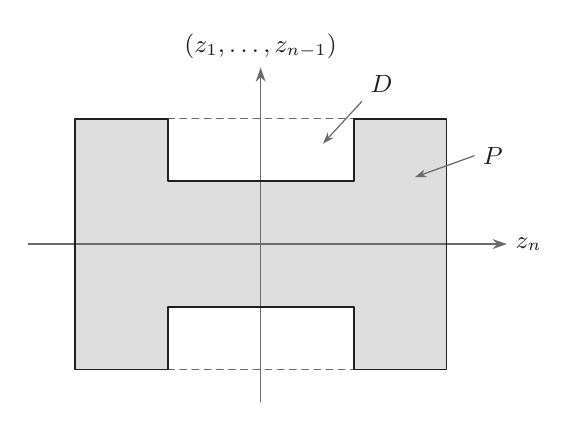
\begin{tikzpicture}[field/diagram, x=1.18cm, y=1.18cm]
    \def\HartogsBoundary{
        (-2,-1.35) -- (-1,-1.35) -- (-1,-0.675)
        -- (1,-0.675) -- (1,-1.35) -- (2,-1.35)
        -- (2,1.35) -- (1,1.35) -- (1,0.675)
        -- (-1,0.675) -- (-1,1.35) -- (-2,1.35) -- cycle
    }
    \fill[FieldRegion] \HartogsBoundary;
    \draw[field/hidden] (-1,1.35) -- (1,1.35)
                        (-1,-1.35) -- (1,-1.35);
    \draw[field/axis] (-2.5,0) -- (2.65,0) node[right] {$z_n$};
    \draw[field/axis] (0,-1.7) -- (0,1.9)
        node[above] {$(z_1,\ldots,z_{n-1})$};
    \draw[field/boundary] \HartogsBoundary;
    \node (D) at (1.3,1.72) {$D$};
    \draw[field/leader] (D.south west) -- (0.67,1.08);
    \node (P) at (2.5,0.95) {$P$};
    \draw[field/leader] (P.west) -- (1.66,0.72);
\end{tikzpicture}

        \FieldCaption{I}{2}{}
    \end{minipage}
\end{center}
We claim that every analytic function on $P$ extends analytically to $D$. Our proof is similar to that of example 1. Suppose $f\in A(P)$, we define
\[F(z_1,\ldots,z_n)=(2\pi i)^{-1}\int_{|\zeta|=3/4}f(z_1,\ldots,z_{n-1},\zeta)/(\zeta-z_n)\,d\zeta,\]
where $|z_i|<1$, $1\leq i\leq n-1$ and $|z_n|<3/4$. Certainly $F$ is analytic and if $|z_1|,\ldots,|z_{n-1}|<\tfrac12$ we see that $F(z_1,\ldots,z_n)=f(z_1,\ldots,z_n)$ by Cauchy's integral formula. It now follows by uniqueness of analytic continuation that $F=f$ wherever both are defined and setting $F=f$ for $1>|z_n|\geq3/4$ we see that $F$ is the required analytic extension of $f$ to $D$. The pair $(D,P)$ is called a \emph{Euclidean Hartogs figure}\IndexMark{idx-280}{hartogs figure@Hartogs figure}\IndexMark{idx-281}{hartogs figure@Hartogs figure!generalised@generalised}.
\begin{enumerate}\setcounter{enumi}{3}
\item Suppose $(D,P)$ is as in example 3 and $g:D\to\mathbb C^n$ is biholomorphic onto the image of $g$. Set $\widetilde D=g(D)$, $\widetilde P=g(P)$. We claim that every analytic function on $\widetilde P$ extends uniquely to an analytic function on $\widetilde D$. Indeed, if $f\in A(\widetilde P)$, $gf\in A(P)$. Now $fg$ extends by example 3 to $F\in A(D)$. Clearly $Fg^{-1}\in A(\widetilde D)$ is the required analytic extension of $f$ to $\widetilde D$. The pair $(\widetilde D,\widetilde P)$ is called a \emph{generalised Hartogs figure}. As we shall see later in this chapter we can use generalised Hartogs figures as a test to determine whether or not every analytic function on a given domain can be extended to a larger domain.
\end{enumerate}
The remainder of this section is devoted to a proving the Theorem of Hartogs referred to in example 2 above. The proof follows Ehrenpreis \cite{bib:I:ehrenpreis-l:1} and H\"ormander \cite{bib:I:hormander-l:1} and uses an existence theorem for the $\partial/\partial\bar z_j$ operators.
% Original book page 56

Suppose $f_j\in C^\infty(\mathbb C^n)$, $j=1,\ldots,n$ and that we wish to solve the system of partial differential equations
\[\partial u/\partial\bar z_j=f_j,\quad 1\leq j\leq n.\]
We first remark that this system is overdetermined in that for solvability the additional conditions
\[\partial f_i/\partial\bar z_j=\partial f_j/\partial\bar z_i,\quad 1\leq i,j\leq n\]
obviously have to be satisfied.
\FieldHeading{Theorem}{2.3.1}{}\FieldTarget{theorem:2.3.1}{2.3.1} Let $f_j\in C_c^\infty(\mathbb C^n)$, $1\leq j\leq n$ and suppose that $\partial f_i/\partial\bar z_j=\partial f_j/\partial\bar z_i$, $1\leq i,j\leq n$. Then the system of equations
\[\partial u/\partial\bar z_j=f_j\]
has a solution $u\in C_c^\infty(\mathbb C^n)$ provided that $n>1$.
\begin{proof}
Define
\[u(z)=(2\pi i)^{-1}\int_{\mathbb C}f_1(\zeta,z_2,\ldots,z_n)/(\zeta-z_1)\,d\zeta\,d\bar\zeta.\]
Changing variables we see that
\[u(z)=-(2\pi i)^{-1}\int_{\mathbb C}f_1(z_1-\zeta,z_2,\ldots,z_n)\zeta^{-1}\,d\zeta\,d\bar\zeta\]
and so $u\in C^\infty(\mathbb C^n)$. Furthermore, since $f_1$ has compact support, $u(z)=0$ provided that $|z_2|+\cdots+|z_n|$ is sufficiently large.

Theorem~\ref{theorem:A1.6} implies that $\partial u/\partial\bar z_1=f_1$. Differentiating under the integral sign with respect to $\bar z_j$ and using the relation $\partial f_j/\partial\bar z_1=\partial f_1/\partial\bar z_j$, we obtain
\begin{align*}
\partial u/\partial\bar z_j&=(2\pi i)^{-1}\int_{\mathbb C}(\zeta-z_1)^{-1}\partial f_j/\partial\bar\zeta(\zeta,z_2,\ldots,z_n)\,d\zeta\,d\bar\zeta\\
&=f_j,\text{ by Theorem~\ref{theorem:A1.2}.}
\end{align*}
Hence $u$ is a solution of the given system of equations. Now let $K$ denote the union of the supports of the $f_j$. Then $u\in A(\mathbb C^n\setminus K)$ and $u$
% Original book page 57
is zero for $|z_2|+\cdots+|z_n|$ sufficiently large. Hence, by uniqueness of analytic continuation, $u$ is zero on the unbounded component of $\mathbb C^n\setminus K$ and so $u$ has compact support.
\end{proof}
\paragraph*{Remarks.}
\begin{enumerate}
\item As we remarked in the appendix to Chapter~\ref{ch:1}, Theorem~\ref{theorem:2.3.1} is false for $n=1$.
\item Later, in Chapter~\ref{ch:5}, we shall rewrite the system of partial differential equations occurring in Theorem~\ref{theorem:2.3.1} in the framework of differential forms.
\end{enumerate}
\FieldHeading{Theorem}{2.3.2}{ (Hartog's theorem).}\FieldTarget{theorem:2.3.2}{2.3.2} Let $\Omega$ be a domain in $\mathbb C^n$, $n>1$, and $K$ be a compact subset of $\Omega$ such that $\Omega\setminus K$ is connected. Then every analytic function on $\Omega\setminus K$ extends uniquely to an analytic function on $\Omega$.
\begin{proof}
Choose $\theta\in C_c^\infty(\Omega)$ so that $\theta\equiv1$ on $K$. Define $f_0\in C^\infty(\Omega)$ by setting
\[f_0|K=0;\quad f_0|\Omega\setminus K=(1-\theta)f.\]
We shall construct $v\in C^\infty(\mathbb C^n)$ so that $f_0+v$ is the required continuation of $f$. First notice that $f_0+v$ will be analytic iff $v$ satisfies
\begin{align*}
\partial v/\partial\bar z_j&=-\partial f_0/\partial\bar z_j,\quad j=1,\ldots,n\\
&=-\partial\theta/\partial\bar z_j f.
\end{align*}
Now $-\partial\theta/\partial\bar z_j f\in C_c^\infty(\mathbb C^n)$ and so we may apply Theorem~\ref{theorem:2.3.1} to find $v\in C_c^\infty(\mathbb C^n)$ such that $f_0+v\in A(\Omega)$. Now observe that since $v$ has compact support, $v$ vanishes on the unbounded component of the complement of the support of $\theta$---uniqueness of analytic continuation. Since $\operatorname{supp}(\theta)\subset\Omega$, there exists an open set in $\Omega\setminus K$ where $v=0$ and so $f=f_0$. Since $\Omega\setminus K$ is connected, $f=f_0+v$ on $\Omega\setminus K$ and so $f_0+v$ is the required analytic extension of $f$.
\end{proof}
\paragraph*{Remark.} An alternative proof of Hartog's theorem, based on\IndexMark{idx-283}{hartogs theorem@Hartogs theorem!extension of analytic functions@extension of analytic functions} the Bochner--Martinelli integral formula, may be found in Bochner \cite{bib:I:bochner-s:1}. See also Harvey \cite[page 355]{bib:I:harvey-f-r:2}.
% Original book page 58
\FieldHeading{Corollary}{2.3.3}{}\FieldTarget{corollary:2.3.3}{2.3.3} Let $\Omega$ be a domain in $\mathbb C^n$, $n>1$, and $f\in A(\Omega)$. Then the zero set $Z(f)$ of $f$ is never a compact subset of $\Omega$.
\begin{proof}
If $Z(f)$ were compact, $1/f\in A(\Omega\setminus Z(f))$ would extend analytically to $\Omega$ by Theorem~\ref{theorem:2.3.2}.
\end{proof}
The corollary emphasises an important difference between the one- and several-variable theory of analytic functions. The zero set of an analytic function of more than one variable always propagates to the boundary of the domain on which the function is defined. It is this essential non-compactness that makes the study of the zero and pole sets so much harder than for functions of one complex variable.
\paragraph*{Exercise.} Let $\Omega,\omega$ be domains in $\mathbb C^n$, $\mathbb C$ respectively. A map $f:\Omega\to\omega$ is said to be \emph{proper} if $f^{-1}(K)$ is compact whenever $K\subset\omega$ is compact. Prove that if $n>1$, there are no proper holomorphic maps of $\Omega$ into $\omega$ (Hint: Let $z_0\in f(\Omega)$ and consider $g(z)=(f(z)-z_0)^{-1}\in A(\Omega\setminus f^{-1}(z_0))$).

\section{Domains of Holomorphy}\label{sec:2:4}
In \hyperref[sec:2:3]{\S3} we gave a large class of examples of domains in $\mathbb C^n$, $n>1$, that possessed the property that every analytic function on them extended to a larger domain. In this section we wish to look at domains where this phenomenon does not happen and the generalisation of Corollary~\ref{corollary:1.3.5} is true.

Throughout this section $\Omega$ will denote a domain in $\mathbb C^n$.
\FieldHeading{Definition}{2.4.1}{}\FieldTarget{definition:2.4.1}{2.4.1} A domain in $\mathbb C^n$ is called a \emph{domain of holomorphy}\IndexMark{idx-210}{domain of holomorphy@Domain of holomorphy} if whenever we are given open connected subsets $U\subset V\subset\mathbb C^n$, with $U\subset\Omega$, such that $f|U$ extends analytically to $V$ for all $f\in A(\Omega)$, then $V\subset\Omega$.

For $\Omega$ to be a domain of holomorphy we require that we cannot extend every analytic function on $\Omega$ locally across any point of the boundary of $\Omega$. We frame the definition in this rather complicated fashion to exclude the following type of domain:
% Original book page 59
\begin{center}
    \begin{minipage}{\linewidth}
        \centering
        % Figure 3. Keep the original domain path and the separate U and V.
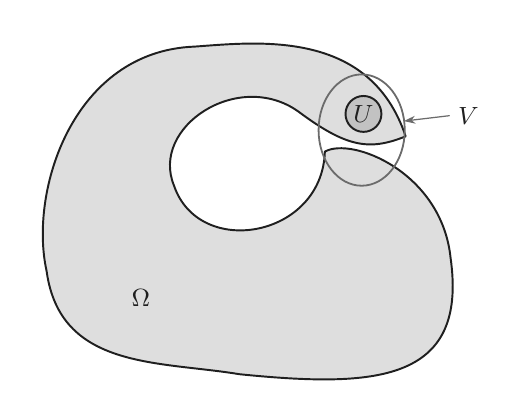
\begin{tikzpicture}[field/diagram, scale=1.14]
    \def\OmegaBoundary{
        (1.55,1.15)
        .. controls (1.15,2.35) and (-0.1,2.2) .. (-0.8,2.15)
        .. controls (-2.15,2.1) and (-2.65,0.55) .. (-2.45,-0.35)
        .. controls (-2.3,-1.45) and (-1.2,-1.35) .. (-0.3,-1.5)
        .. controls (1.2,-1.65) and (2.25,-1.6) .. (2.05,-0.2)
        .. controls (1.95,0.75) and (0.95,1.15) .. (0.65,0.98)
        .. controls (0.62,0.02) and (-0.75,-0.22) .. (-1.03,0.6)
        .. controls (-1.3,1.25) and (-0.32,1.9) .. (0.35,1.43)
        .. controls (0.9,1.02) and (1.15,0.99) .. (1.55,1.15)
        -- cycle
    }
    \fill[FieldRegion, even odd rule] \OmegaBoundary;
    \draw[field/boundary] \OmegaBoundary;
    \draw[field/secondary] (1.06,1.22) ellipse (0.48 and 0.62);
    \filldraw[fill=FieldEmphasis, field/boundary]
        (1.08,1.4) circle (0.20);
    \node[inner sep=0.5pt] at (1.08,1.4) {$U$};
    \node (V) at (2.25,1.38) {$V$};
    \draw[field/leader] (V.west) -- (1.53,1.32);
    \node at (-1.4,-0.65) {$\Omega$};
\end{tikzpicture}

        \FieldCaption{I}{3}{}
    \end{minipage}
\end{center}
Referring to the figure, suppose that $f|U$ extends to $F\in A(V)$ for all $f\in A(\Omega)$. Then $\Omega$ will not be a domain of holomorphy. Notice though that $F|\Omega\cap V$ need not equal $f|\Omega\cap V$---we give an explicit example below.
\paragraph*{Examples.}
\begin{enumerate}
\item $\mathbb C^n$ is a domain of holomorphy, $n\geq1$.
\item If $K$ is a compact subset of $\Omega\subset\mathbb C^n$, $n>1$, such that $\Omega\setminus K$ is connected then $\Omega\setminus K$ is not a domain of holomorphy (Theorem~\ref{theorem:2.3.2}).
\item Every domain $\Omega$ in $\mathbb C$ is a domain of holomorphy. This is trivial: Given $a\in\partial\Omega$, define $f(z)=(z-a)^{-1}\in A(\Omega)$ and observe that $f$ cannot extend to any open neighbourhood of $a$.
\item A necessary condition for $\Omega$ to be a domain of holomorphis is that if $(\widetilde D,\widetilde P)$ is any generalised Hartog's figure (Example 4, \hyperref[sec:2:3]{\S3}) with $\widetilde P\subset\Omega$, then $\widetilde D\subset\Omega$. Actually this condition turns out to be sufficient (see the discussion in \hyperref[sec:2:5]{\S5}).
\item Given open domains $U_i\subset\mathbb C$, $1\leq i\leq n$, $U=\prod_{i=1}^n U_i$ is a domain of holomorphy. Indeed, $\partial U=\bigcup_i U_1\times\cdots\times\partial U_i\times\cdots\times U_n$ and so if $a=(a_1,\ldots,a_n)\in\partial U$, we must have at least one $a_i\in\partial U_i$. Now define $f(z_1,\ldots,z_n)=(z_i-a_i)^{-1}$. Clearly $f$ does not extend to any open neighbourhood of $a$. Alternatively, choose $f_i\in A(U_i)$ satisfying the conditions of Corollary~\ref{corollary:1.3.5}. Define $f(z_1,\ldots,z_n)=\sum_{i=1}^n f_i(z_i)$. In this case we see that $U$ is the ``domain of existence'' for $f$.
% Original book page 60
\item Let $V=\{z\in D(0;1):z_1=\cdots=z_{n-1}=0,\ \operatorname{Im}(z_n)=0,\ \operatorname{Re}(z_n)\geq0\}$ and set $\Omega=D(0;1)\setminus V$. Every analytic function on $\Omega$ extends analytically to $D(0;1)$ (Exercise 2, \hyperref[sec:2:2]{\S2} or use Laurent series at 0). On the other hand $\Omega$ is homeomorphic to $D(0;1)$ and so we see that the property of being a domain of holomorphy is not a topological invariant.
\item We now present an example to show that the phenomenon alluded to after definition 2.4.1 can occur. Our example is in $\mathbb C^2$, though it is easily generalised to $\mathbb C^n$, $n>2$. Let $A\subset\mathbb C^2$ be the product of the ``cut'' annulus $\{z\in\mathbb C:\tfrac12<|z-2|<3/2\}\setminus\{z\in\mathbb C:|z|=\tfrac12\text{ and }\arg(z)\in(0,\pi)\}$ with the disc $|w|<\tfrac14$. We define $\Omega$ to be the union of $A$ with $P=\{(z,w)\in D(0;1):|z|<\tfrac12\text{ or }1>|w|>\tfrac12\}$. Let $D=D(0;1)$.
\begin{center}
    \begin{minipage}{\linewidth}
        \centering
        % Figure 4. A cut annulus and the overlapping Hartogs set P.
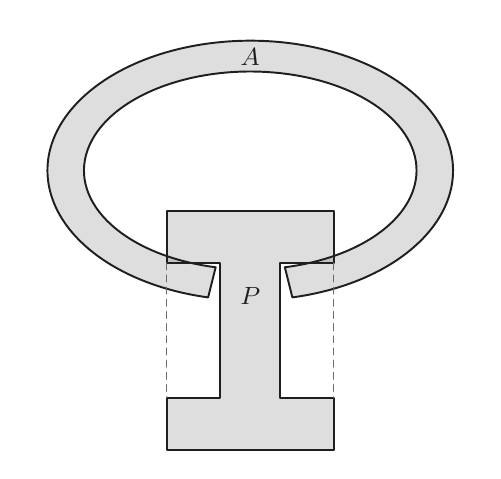
\begin{tikzpicture}[field/diagram, scale=1.03]
    \def\CutAnnulus{
        ({2.5*cos(-78)},{1.8+1.6*sin(-78)})
        arc[start angle=-78, end angle=258, x radius=2.5, y radius=1.6]
        -- ({2.05*cos(258)},{1.8+1.22*sin(258)})
        arc[start angle=258, end angle=-78, x radius=2.05, y radius=1.22]
        -- cycle
    }
    \def\HartogsBoundary{
        (-1.03,1.3) -- (1.03,1.3) -- (1.03,0.66)
        -- (0.37,0.66) -- (0.37,-1.0) -- (1.03,-1.0)
        -- (1.03,-1.65) -- (-1.03,-1.65) -- (-1.03,-1.0)
        -- (-0.37,-1.0) -- (-0.37,0.66) -- (-1.03,0.66) -- cycle
    }
    \fill[FieldRegion] \CutAnnulus;
    \fill[FieldRegion] \HartogsBoundary;
    % Darker gray records the actual overlap, not an additional set.
    \begin{scope}
        \clip \CutAnnulus;
        \fill[FieldEmphasis] \HartogsBoundary;
    \end{scope}
    \draw[field/boundary] \CutAnnulus;
    \draw[field/boundary] \HartogsBoundary;
    \draw[field/hidden] (-1.03,0.66) -- (-1.03,-1.0)
                        (1.03,0.66) -- (1.03,-1.0);
    \node[inner sep=0.5pt] at (0,3.20) {$A$};
    \node at (0,0.25) {$P$};
\end{tikzpicture}

        \FieldCaption{I}{4}{}
    \end{minipage}
\end{center}
Since $(D,P)$ is a Euclidean Hartog's figure, $f|P$ extends analytically to $F\in A(D)$ for all $f\in A(\Omega)$. But in general $F|D\cap\Omega\neq f|D\cap\Omega$ as is seen by taking $f(z,w)=\sqrt{(z-2)}$.
\end{enumerate}
% Original book page 61
Example 5 suggests that a domain of holomorphy might be the domain of existence of an analytic function (note that the converse is trivially true). Much of the remainder of this section will be devoted to proving that every domain of holomorphy is the domain of existence of some analytic function. In the course of our proof we shall derive other important characterizations of domains of holomorphy.

Example 3 and 5 also suggest that if $\Omega$ is a domain of holomorphy, $z\in\partial\Omega$ and $(z_n)\subset\Omega$ converges to $z$, then there exists $f\in A(\Omega)$ which is unbounded on the sequence $(z_n)$. We make a formal definition.
\FieldHeading{Definition}{2.4.2}{}\FieldTarget{definition:2.4.2}{2.4.2} We say that the domain $\Omega$ possesses property (S\IndexMark{idx-477}{property s@Property (S)}) if given any sequence $(z_n)\subset\Omega$ which converges to a point $z\in\partial\Omega$, there exists $f\in A(\Omega)$ which is unbounded on the sequence $(z_n)$.
\FieldHeading{Lemma}{2.4.3}{}\FieldTarget{lemma:2.4.3}{2.4.3} If the domain $\Omega$ possesses property (S), $\Omega$ is a domain of holomorphy.
\begin{proof}
Suppose $\Omega$ is not a domain of holomorphy. Then there exists $z\in\partial\Omega$ and open connected sets $U\subset V\subset\mathbb C^n$ such that $U\subset\Omega$, $z\in V$ and $f|U$ extends to $F\in A(V)$ for every $f\in A(\Omega)$. Now let $(z_n)\subset\Omega\cap V$ converge to $z$. We see immediately that $F$ is bounded on $(z_n)$. Therefore $f$ is bounded on $(z_n)$ for all $f\in A(\Omega)$ and $\Omega$ does not possess property (S).
\end{proof}
\paragraph*{Examples.}
\begin{enumerate}\setcounter{enumi}{6}
\item The Euclidean disc $E=\{z\in\mathbb C^n:\sum_{i=1}^n|z_i|^2<r^2\}$ is a domain of holomorphy. We show $E$ possesses property (S). Suppose $a=(a_1,\ldots,a_n)\in\partial E$. Define $f(z)=(r^2-\langle z,a\rangle)^{-1}$, where $\langle\ ,\ \rangle$ denotes the standard Hermitian inner product on $\mathbb C^n$. Clearly $f\in A(E)$ and $f$ is not bounded on any sequence of points of $E$ converging to $a$.
\item Let $f_j\in A(\mathbb C^n)$, $1\leq j\leq q$. The \emph{analytic polyhedron}\IndexMark{idx-020}{analytic polyhedron@Analytic polyhedron} $P=\{z\in\mathbb C^n:|f_j(z)|<1,\ 1\leq j\leq q\}$ possesses property (S) and is a domain of holomorphy. Indeed, if $a\in\partial P$, $|f_i(a)|=1$ for some $i$. Now define $F(z)=(f_i(z)-f_i(a))^{-1}\in A(P)$. Clearly $F$ is not bounded on any sequence of points of $P$ converging to $a$.
\end{enumerate}
It turns out that in some ways domains of holomorphy are the complex analogue of convex sets. The next definition reflects these
% Original book page 62
convexity properties particularly well. Before giving the definition we recall that if $K$ is a compact subset of $\Omega\subset\mathbb C^n$ and $f:\Omega\to\mathbb C$, then $\|f\|_K$ is, by definition, $\sup_{z\in K}|f(z)|$.
\FieldHeading{Definition}{2.4.4}{}\FieldTarget{definition:2.4.4}{2.4.4} A domain $\Omega$ is said to be \emph{holomorphically convex}\IndexMark{idx-292}{holomorphic convexivity@Holomorphic convexivity} if given any compact subset $K\subset\Omega$ the set
\[\widehat K=\{z\in\Omega:|f(z)|\leq\|f\|_K\text{ for all }f\in A(\Omega)\}\]
is compact.
\paragraph*{Remark.} We call $\widehat K$ the $A(\Omega)$-hull of $K$. If $K=\widehat K$, we say $K$ is $A(\Omega)$-convex.
\paragraph*{Examples.}
\begin{enumerate}\setcounter{enumi}{8}
\item Every domain $\Omega$ in $\mathbb C$ is holomorphically convex. In fact it is easy to see that $d(K,\partial\Omega)=d(\widehat K,\partial\Omega)$ for every compact subset $K$ of $\Omega$: Just consider functions $f(z)=(z-\zeta)^{-1}\in A(\Omega)$, where $\zeta\in\partial\Omega$.
\item The domain $\mathbb C^n\setminus\{0\}$, $n>1$, is not holomorphically convex. Indeed suppose $K=\{z\in\mathbb C^n:|z|=1\}$ (the boundary of the unit polydisc). Then $\widehat K=\{z:0<|z|\leq1\}$ (the punctured unit polydisc). To see this we notice that by Theorem~\ref{theorem:2.3.2} any $f\in A(\mathbb C^n\setminus\{0\})$ extends to $F\in A(\mathbb C^n)$. By the Maximum Principle (Theorem~\ref{theorem:2.1.12}), the maximum value of $F$ on $\{z:|z|\leq1\}$ is taken on its boundary, $K$. Since $F$ is an extension of $f$ the same is true for $f$. This implies $\widehat K\supseteq\{z:0<|z|\leq1\}$. The reverse inclusion is trivial. Notice that if $n=1$, $\widehat K=K$ as is seen by taking $f(z)=z^{-1}$.
\end{enumerate}
Before stating the next lemma we wish to review a few elementary facts about convex subsets of $\mathbb R^n$. Suppose $X\subset\mathbb R^n$. We say that $X$ is \emph{convex} if, given $x,y\in X$, $tx+(1-t)y\in X$ for all $t\in[0,1]$. Now suppose $X$ is bounded. The (closed) \emph{convex hull}\IndexMark{idx-137}{convex hull closed@Convex hull (closed)}, $X_c$, of $X$ is defined to be
\[X_c=\{u\in\mathbb R^n:\phi(u)\leq\sup_{x\in X}\phi(x)\text{ for all }\phi\in\mathbb R^{n\prime}\}.\]
The following properties of the convex hull are easily verified:
% Original book page 63
\begin{gather*}
X_c\text{ is closed, convex and bounded}\\
X_{cc}=X_c\\
X_c\supset X\text{ and }X_c\text{ is the smallest closed convex set containing }X\\
X_c=X\text{ if and only if }X\text{ is closed and convex.}
\end{gather*}
\FieldHeading{Lemma}{2.4.5}{}\FieldTarget{lemma:2.4.5}{2.4.5} Let $K$ be a compact subset of the domain $\Omega$ in $\mathbb C^n$. Then
\begin{enumerate}
\item $\widehat K\supset K$.
\item $\widehat K$ is a closed subset of $\Omega$.
\item $\widehat{\widehat K}=\widehat K$.
\item $\widehat K\subset K_c$. In particular, $\widehat K$ is bounded.
\end{enumerate}
\begin{proof}
1, 2 and 3 are trivial. Let us prove 4.
\[K_c=\{u\in\mathbb C^n:\phi(u)\leq\sup_{z\in K}\phi(z)\text{ for all }\phi\in L_{\mathbb R}(\mathbb C^n,\mathbb R)\}.\]
Given $\phi\in L_{\mathbb R}(\mathbb C^n,\mathbb R)$, we may write
\[\phi(z_1,\ldots,z_n)=\sum_{i=1}^n a_i z_i+\sum_{i=1}^n b_i\bar z_i\]
where $a_i,b_i\in\mathbb C$. Since $\phi$ is real valued we must have $b_i=\bar a_i$, $i=1,\ldots,n$, and so
\[\phi(z_1,\ldots,z_n)=2\operatorname{Re}\sum_{i=1}^n a_i z_i.\]
Define $f(z)=\exp(2\sum_{i=1}^n a_i z_i)\in A(\Omega)$. If $z\in\widehat K$,
\[|f(z)|\leq\|f\|_K.\]
That is,
\[|\exp\phi(z)|\leq\|\exp\phi\|_K,\text{ since }|f(z)|=|\exp\phi(z)|.\]
This implies $\phi(z)\leq\sup_K\phi$, since $\phi$ is real. Hence $z\in K_c$.
\end{proof}
% Original book page 64
\paragraph*{Remark.} The reader should note the close analogy between properties of the $A(\Omega)$-hull and the convex hull. It should also be noted that an open subset $\Omega$ of $\mathbb R^n$ is convex if and only if $K_c$ is a compact subset of $\Omega$ for every compact subset $K$ of $\Omega$. Furthermore, convexivity is a local property of the boundary of $\Omega$ (Every disc centered on the boundary of $\Omega$ meets $\Omega$ in a convex set if $\Omega$ is convex and this property characterises the convexivity of $\Omega$). We shall see in \hyperref[sec:2:5]{\S5} that we can also formulate holomorphic convexivity in terms of local properties of the boundary.
\FieldHeading{Theorem}{2.4.6}{}\FieldTarget{theorem:2.4.6}{2.4.6} A domain $\Omega$ in $\mathbb C^n$ is holomorphically convex if and only if it possesses property (S). In particular, if $\Omega$ is holomorphically convex it is a domain of holomorphy.
\begin{proof}
We start by showing that (S) implies holomorphic convexivity. Suppose $\Omega$ possesses property (S). If $\Omega$ is not holomorphically convex there exists a compact subset $K$ of $\Omega$ such that $\widehat K$ is not compact. Since $\widehat K$ is bounded we can therefore find a sequence $(z_n)\subset\widehat K$ which converges to some point of $\partial\Omega$. Now $|f(z_n)|\leq\|f\|_K$ for all $f\in A(\Omega)$ by definition of $\widehat K$. Hence every $f\in A(\Omega)$ must be bounded on $(z_n)$. This is contrary to our assumption that $\Omega$ possesses property (S) and so $\Omega$ is holomorphically convex.

Suppose $\Omega$ is holomorphically convex. Let $(z_n)\subset\Omega$ be a sequence converging to some point of $\partial\Omega$. It is sufficient to construct $f\in A(\Omega)$ which is unbounded on $(z_n)$.

First we choose a sequence $(K_n)$ of compact subsets of $\Omega$ satisfying
\begin{enumerate}
\item $K_n\subset K_{n+1}$, $n\geq1$.
\item $\bigcup_n K_n=\Omega$.
\item $K_n=\widehat K_n$, $n\geq1$.
\item Every point of $\Omega$ is an interior point of some $K_n$.
\end{enumerate}
To see that such sequences exist, we first construct a sequence $K'_n$ of compact subsets of $\Omega$ satisfying 1, 2 and 4 just as in the proof of Theorem~\ref{theorem:A1.8}. We then define $K_n=\widehat K'_n$ and note that 1 continues to hold since the operation of forming the $A(\Omega)$-hull clearly preserves inclusions.
% Original book page 65
Notice that condition 4 implies that every compact subset of $\Omega$ is contained in $K_n$ for $n$ sufficiently large.

Choose an infinite subsequence $(x_k)$ of $(z_n)$ which possesses the property that $x_k\in K_{n(k)+1}\setminus K_{n(k)}$, $k\geq1$, where the sequence $(n(k))$ is strictly increasing. We leave the construction of such a sequence as an easy exercise for the reader (note that $(K_{n+1}-K_n)\cap(z_n)$ is always finite). It is clearly enough to construct $f\in A(\Omega)$ which is unbounded on $(x_k)$. For $k\geq1$, let $L_k=K_{n(k)}$, $\|g\|_k=\|g\|_{L_k}$ and observe that the sequence $(L_k)$ satisfies conditions 1 to 4 above.

We construct inductively a sequence $f_k\in A(\Omega)$ satisfying
\[f_k(x_k)=k+1+\sum_{j=1}^{k-1}|f_j(x_k)|\quad\text{and}\quad\|f_k\|_k\leq2^{-k+2}.\tag{*}\label{eq:2:star:1}\]
Take $f_1\equiv2$. Suppose $f_1,\ldots,f_{k-1}$ are constructed. Since $x_k\notin L_k$, there exists $g\in A(\Omega)$ such that $|g(x_k)|>\|g\|_k$. Dividing by $g(x_k)$ we may assume
\[1=g(x_k)>\|g\|_k.\]
Choose $p(k)$ so large that
\[\|g^{p(k)}\|_k\leq2^{-k+2}/\left(k+1+\sum_{j=1}^{k-1}|f_j(x_k)|\right).\]
Set $f_k=(k+1+\sum_{j=1}^{k-1}|f_j(x_k)|)g^{p(k)}$. The inductive step is completed. We now define
\[f=\sum_{k=1}^\infty f_k.\]
Conditions \eqref{eq:2:star:1} imply that the sum converges uniformly on $L_k$ for $k\geq1$ (compare with the proof of Theorem~\ref{theorem:A1.8}) and also that $|f(x_k)|\geq k-1$, $k\geq1$. Since every compact subset of $\Omega$ is contained in $L_k$ for $k$ large enough it follows by Corollary~\ref{corollary:2.1.8} that $f\in A(\Omega)$. Since $f$ is unbounded on $(x_k)$ the proof is complete.
\end{proof}
% Original book page 66
\paragraph*{Remarks.}
\begin{enumerate}
\item The technique used to construct the function in the second part of the proof is very effective and we use it again shortly. Holomorphic convexivity is well adapted to the construction of analytic functions.
\item The sequence $(K_n)$ of compact subsets of $\Omega$ constructed in the proof of Theorem~\ref{theorem:2.4.6} is called a \emph{normal exhaustion}\IndexMark{idx-408}{normal exhaustion@Normal exhaustion} of $\Omega$.
\end{enumerate}
\paragraph*{Example 11.} Any open convex subset of $\mathbb C^n$ is a domain of holomorphy. Indeed, since $\widehat K\subset K_c$, any open convex subset of $\mathbb C^n$ must be holomorphically convex. Of course, using the technique of the proof of Lemma~\ref{lemma:2.4.5}, it can easily be proved directly that an open convex subset of $\mathbb C^n$ is a domain of holomorphy.
\paragraph*{Remark.} Holomorphic convexivity is much weaker than convexivity: Any open subset of $\mathbb C$ is holomorphically convex as are products of open subsets of $\mathbb C$.
\FieldHeading{Definition}{2.4.7}{}\FieldTarget{definition:2.4.7}{2.4.7} Let $f\in A(\Omega)$. We say that $\Omega$ is the \emph{domain of existence}\IndexMark{idx-209}{domain of existence@Domain of existence} of $f$, if $f$ cannot be analytically continued across any point of the boundary of $\Omega$.
\paragraph*{Remarks.}
\begin{enumerate}
\item Every domain of existence is trivially a domain of holomorphy.
\item If $\Omega$ is a domain in $\mathbb C$ then $\Omega$ is a domain of existence by Corollary~\ref{corollary:1.3.5}.
\end{enumerate}
\FieldHeading{Theorem}{2.4.8}{}\FieldTarget{theorem:2.4.8}{2.4.8} Every holomorphically convex domain $\Omega$ in $\mathbb C^n$ is the domain of existence of some analytic function on $\Omega$.
\begin{proof}
Our proof is rather similar to that of Theorem~\ref{theorem:2.4.6}.

Let $(K_n)$ be a normal exhaustion of $\Omega$ and $M$ be a discrete subset of $\Omega$ such that $\bar M\supset\partial\Omega$ (see the proof of Corollary~\ref{corollary:1.3.5} for the construction of $M$). For each $n\geq1$, there exist only finitely many points of $M$ in $K_{n+1}\setminus K_n$, say $x_1,\ldots,x_p$. As in the proof of Theorem~\ref{theorem:2.4.6} there exist $g_1,\ldots,g_p\in A(\Omega)$ such that
\[1=g_1(x_1)=\cdots=g_p(x_p)>\|g_1\|_{K_n},\ldots,\|g_p\|_{K_n}.\]
% Original book page 67
By perturbing each $g_j$ by a term $\theta(z-x_j)$, where $\theta\in\mathbb C^{n*}$ is small, it is clear that we can assume that $|g_j(x_k)|\neq1$, $j\neq k$.

Set $a_{jk}(z)=(g_j(z)-g_j(x_k))/(1-g_j(x_k))$, $j\neq k$. Taking sufficiently high powers of the $g_j$'s, we may further require that
\[\|g_j\|_{K_n}\leq2^{-n-p}/p\quad\text{and}\quad\|a_{jk}\|_{K_n}\leq2.\]
We now define
\[f_n(z)=\sum_{j=1}^p\left(\prod_{k\neq j}a_{jk}(z)\right)g_j(z),\quad z\in\Omega.\]
Our estimates imply that
\[f_n(x_i)=1,\quad1\leq i\leq p\]
\[\|f_n\|_{K_n}\leq2^{-n}.\]
Define
\[f=\prod_{n=1}^\infty(1-f_n)^n.\]
Since $\sum_{n=1}^\infty n2^{-n}$ is convergent, the infinite product converges uniformly on compact subsets of $\Omega$ and so $f\in A(\Omega)$. The convergence of the infinite product together with the fact that no $f_n$ is identically equal to 1 implies that $f$ is not identically zero.

Let $(x_k)\subset M$ be a sequence converging to $x\in\partial\Omega$. If $x_k\in K_{n(k)+1}\setminus K_{n(k)}$, $f$ and its first $n(k)$ derivatives vanish at $x_k$. Since $n(k)\to\infty$ as $k\to\infty$, we see that any analytic extension of $f$ to a neighbourhood of $x$ would have all its derivatives vanishing at $x$. But this implies, by uniqueness of analytic continuation, that $f\equiv0$. Hence $f$ does not extend across any point of $\partial\Omega$ and $\Omega$ is the domain of existence of $f$.
\end{proof}
\paragraph*{Remark.} Using the method of proof of Theorems~\ref{theorem:2.4.6}, \ref{theorem:2.4.8} it is not hard to show that if $M$ is an infinite discrete subset of a holomorphically convex domain $\Omega$, then there exists $f\in A(\Omega)$ which is unbounded on \emph{every} infinite subset of $M$. Clearly this very strong form of Property (S) implies Theorem~\ref{theorem:2.4.8} as well as the non-trivial part of Theorem~\ref{theorem:2.4.6}.
% Original book page 68

Let us summarise what we have proved so far. We have shown that for a domain $\Omega$ in $\mathbb C^n$, Property (S) is equivalent to holomorphic convexivity. We have also proved that if $\Omega$ is holomorphically convex then $\Omega$ is a domain of existence which in turn implies that $\Omega$ is a domain of holomorphy. We next show that these four properties are equivalent by proving that every domain of holomorphy is holomorphically convex.

First some notation. If $K\subset\Omega$ is compact, we let
\begin{align*}
d_\Omega(K)&=d(\partial\Omega,K)\\
&=\inf\{|z-\zeta|:z\in\partial\Omega,\ \zeta\in K\}.
\end{align*}
Provided that $\Omega\neq\mathbb C^n$, $d_\Omega(K)<\infty$. We remark that if $d(z,\partial\Omega)=r$ and $z\in\Omega$, then $D(z;r)\subset\Omega$ and indeed is the largest open polydisc $D(z;s)$ contained in $\Omega$ and centered at $z$.
\FieldHeading{Proposition}{2.4.9}{}\FieldTarget{proposition:2.4.9}{2.4.9} Let $K$ be a compact subset of $\Omega\subset\mathbb C^n$ and $z_0\in\widehat K$. If $f\in A(\Omega)$, the power series for $f$ at $z_0$,
\[f(z)=\sum_m\frac1{m!}\partial^m f(z_0)(z-z_0)^m,\]
converges on $D(z_0;d_\Omega(K))$.
\begin{proof}
Choose $r$, $0<r<d_\Omega(K)$ and define $K_r=\bigcup_{z\in K}\bar D(z;r)$. $K_r$ is certainly compact and contained in $\Omega$. Let $M=\|f\|_{K_r}$. By Corollary~\ref{corollary:2.1.8} applied to $\bar D(z;r)$ we have
\[|\partial^m f(z)|\leq Mm!r^{-|m|}\]
for $z\in K$ ($|m|=m_1+\cdots+m_n$). Hence
\[\|\partial^m f\|_K\leq Mm!r^{-|m|}.\]
Since $\partial^m f\in A(\Omega)$ we have, by definition of $\widehat K$,
\[\|\partial^m f\|_{\widehat K}\leq Mm!r^{-|m|}.\]
Since $z_0\in\widehat K$, this estimate implies
% Original book page 69
\[|\partial^m f(z_0)|\leq Mm!r^{-|m|}\]
and so the series $\sum\frac1{m!}\partial^m f(z_0)(z-z_0)^m$ converges for $|z-z_0|<r$. Since this is true for all $r<d_\Omega(K)$, the Proposition follows.
\end{proof}
\FieldHeading{Theorem}{2.4.10}{ (Cartan--Thullen).}\IndexMark{idx-064}{cartan thullen theorem@Cartan--Thullen theorem}\FieldTarget{theorem:2.4.10}{2.4.10} A domain of holomorphy is holomorphically convex.
\begin{proof}
It is clearly enough to prove that for any compact subset $K$ of a domain of holomorphy $\Omega$, $d_\Omega(K)=d_\Omega(\widehat K)$. Obviously $d_\Omega(K)\geq d_\Omega(\widehat K)$. Suppose that for some compact subset $K$ of $\Omega$, $d_\Omega(K)>d_\Omega(\widehat K)$. Pick $z_0\in\widehat K$ such that $d(z_0,\partial\Omega)<d_\Omega(K)$. By Proposition~\ref{proposition:2.4.9}, $\sum\frac1{m!}\partial^m f(z_0)(z-z_0)^m$ converges on $D(z_0;d_\Omega(K))$. But $D(z_0;d_\Omega(K))\not\subset\Omega$ (see remarks immediately preceding Proposition~\ref{proposition:2.4.9}). Hence we have constructed an analytic extension of every $f\in A(\Omega)$ to some open set not contained in $\Omega$. Contradiction. Hence $\Omega$ is holomorphically convex.
\end{proof}
\paragraph*{Examples.}
\begin{enumerate}\setcounter{enumi}{11}
\item Suppose $\Omega,\Omega'\subset\mathbb C^n$ and $f:\Omega\to\Omega'$ is biholomorphic. If one of $\Omega$, $\Omega'$ is a domain of holomorphy so is the other. This follows since holomorphic convexivity is obviously preserved by biholomorphic maps. Notice that it is \emph{not} obvious from the definitions that domains of holomorphy or existence are preserved by biholomorphic maps.
\item Suppose that $\Omega\subset\mathbb C^n$, $\Omega'\subset\mathbb C^m$ are domains of holomorphy and $f:\Omega\to\mathbb C^m$ is analytic. Then $f^{-1}(\Omega')$ is a domain of holomorphy. We show that $f^{-1}(\Omega')$ possesses property (S). Let $(z_n)$ be a sequence of points of $f^{-1}(\Omega')$ converging to some point $z\in\partial f^{-1}(\Omega')$. If $z\in\partial\Omega$, then there exists $g\in A(\Omega)$ which is unbounded on $(z_n)$. Restricting to $f^{-1}(\Omega')$, we have found an analytic function on $f^{-1}(\Omega')$ unbounded on $(z_n)$. If $z\notin\partial\Omega$, then $(f(z_n))$ converges to $f(z)\in\mathbb C^m$. Clearly, $f(z)\in\partial\Omega'$, and so there exists $g\in A(\Omega')$ which is unbounded on $(f(z_n))$. But then $gf\in A(f^{-1}(\Omega'))$ is unbounded on $(z_n)$. We remark that we can weaken the conditions on $\Omega$ to require only that $\Omega$ possesses property (S) at all points of $\partial\Omega\cap\partial f^{-1}(\Omega')$.
\item Let $\Omega\subset\mathbb C^n$ be a domain of holomorphy and $f_1,\ldots,f_q\in A(\Omega)$\IndexMark{idx-021}{analytic polyhedron@Analytic polyhedron}. Then $P=\{z\in\Omega:|f_j(z)|<1,\ j=1,\ldots,q\}$ is a domain of holomorphy. Indeed,
% Original book page 70
set $f=(f_1,\ldots,f_q):\Omega\to\mathbb C^q$. Then $P=f^{-1}(D(0;1))$ and example 13 applies. We recall that $P$ is an analytic polyhedron.
\item Let $\Omega_i\subset\mathbb C^n$, $i\in I$, be domains of holomorphy. Then $\Omega=\operatorname{Interior}(\bigcap_{i\in I}\Omega_i)$ is a domain of holomorphy. We prove that $\Omega$ is holomorphically convex. Let $K$ be a compact subset of $\Omega$ and $\widehat K$ and $\widehat K_i$ respectively denote the $A(\Omega)$- and $A(\Omega_i)$-hulls of $K$. Certainly $\widehat K\subset\widehat K_i$, $i\in I$. Hence, with the notation of Theorem~\ref{theorem:2.4.10}, $d_\Omega(K)\leq d_{\Omega_i}(\widehat K)$, $i\in I$. This being true for all $i\in I$, we must have $d_\Omega(\widehat K)\geq d_\Omega(K)$ and so $\widehat K$ is a compact subset of $\Omega$.
\end{enumerate}
\paragraph*{Exercises.}
\begin{enumerate}
\item Let $\Omega$ be a domain of holomorphy and $M$ be an infinite discrete subset of $\Omega$. Show that there exists an analytic function on $\Omega$ which is unbounded on every infinite subset of $M$ (see the remarks following Theorem~\ref{theorem:2.4.8}).
\item Let $\Omega$ be holomorphically convex. Show that there exist normal exhaustions\IndexMark{idx-409}{normal exhaustion@Normal exhaustion} $(K_n)$ of $\Omega$ that satisfy the additional property $K_n\subset\mathring K_{n+1}$, $n\geq1$.
\end{enumerate}

\section{Pseudoconvexivity}\label{sec:2:5}
The results of \hyperref[sec:2:4]{\S4} show that there is a close parallel between the convexivity of domains in $\mathbb R^n$ and holomorphic convexivity of domains in $\mathbb C^n$. In this section we shall explore this analogy further. First we shall review some facts about convex domains in $\mathbb R^n$. A standard reference is Bonnesen and Fenchel \cite{bib:I:bonnesen-t-and-fenchel-w:1}.

Let $\Omega$ be a proper subdomain of $\mathbb R^n$ and suppose $\partial\Omega$ is a $C^r$ submanifold of $\mathbb R^n$, $r\geq1$. Using partitions of unity it is not hard to construct $\phi\in C^r(\mathbb R^n,\mathbb R)$ satisfying
\begin{enumerate}
\item[A)] $\Omega=\{x\in\mathbb R^n:\phi(x)<0\}$
\item[B)] $\partial\Omega=\{x\in\mathbb R^n:\phi(x)=0\}$
\item[C)] $d\phi\neq0$ on $\partial\Omega$.
\end{enumerate}
% Original book page 71
We call a map $\phi$ satisfying these conditions a ($C^r$-) defining function for $\Omega$. The following technical lemma will be important in defining boundary invariants of $\Omega$.
\FieldHeading{Lemma}{2.5.1}{}\FieldTarget{lemma:2.5.1}{2.5.1} Let $\Omega$ be a proper subdomain of $\mathbb R^n$ with $C^2$ boundary and suppose that $\phi$ and $\theta$ are defining functions for $\Omega$. Then there exists $h\in C^1(\mathbb R^n,\mathbb R)$ satisfying
\begin{enumerate}
\item[a)] $\phi=h.\theta$
\item[b)] $h$ is strictly positive
\item[c)] $h$ is $C^2$ off $\partial\Omega$
\item[d)] Given $1\leq i,j\leq n$, let
\[a_{ij}(x)=\begin{cases}d(x,\partial\Omega)\dfrac{\partial^2h}{\partial x_i\partial x_j}(x),&x\notin\partial\Omega,\\0,&x\in\partial\Omega.\end{cases}\]
Then $a_{ij}$ is continuous.
\end{enumerate}
($d(x,\partial\Omega)$ is the distance from $x$ to $\partial\Omega$, relative to some norm on $\mathbb R^n$).
\begin{proof}
Clearly we may define $h=\phi/\theta$ on $\mathbb R^n\setminus\partial\Omega$ and $h$ is $C^2$ on $\mathbb R^n\setminus\partial\Omega$. The problem is to show that $h$ extends as a positive $C^1$ function across $\partial\Omega$ satisfying property d). Fix $z\in\partial\Omega$. It is enough to find an open neighbourhood $U$ of $z$ in $\mathbb R^n$ and $h\in C^1(U,\mathbb R)$ such that $h$ satisfies properties a)--d) in $U$. Choose local coordinates on some open neighbourhood $U$ of $z$ so that $z$ corresponds to zero, $\partial\Omega\cap U=\{x\in U:x_1=0\}$ and, in the new coordinates, $U$ is convex. In the new coordinate system we have $\phi(0,x_2,\ldots,x_n)=0$ and $\frac{\partial\phi}{\partial x_1}(0,x_2,\ldots,x_n)\neq0$ for $(0,x_2,\ldots,x_n)\in U$. Similarly for $\theta$. Now
\begin{align*}
\phi(x_1,\ldots,x_n)&=\int_0^1\frac{d}{dt}(\phi(tx_1,\ldots,x_n))\,dt\\
&=\int_0^1x_1\frac{\partial\phi}{\partial x_1}(tx_1,\ldots,x_n)\,dt\\
&=x_1\widetilde\phi(x_1,\ldots,x_n).
\end{align*}
Since $\frac{\partial\phi}{\partial x_1}(0,x_2,\ldots,x_n)\neq0$, $\widetilde\phi(0,x_2,\ldots,x_n)\neq0$ on $\partial\Omega\cap U$. Furthermore $\widetilde\phi$ is $C^1$ on $U$. Similarly, $\theta(x_1,\ldots,x_n)=x_1\widetilde\theta(x_1,\ldots,x_n)$ and so we may extend $h$ to a $C^1$ function on $U$ by setting $h=\widetilde\phi/\widetilde\theta$.
% Original book page 72

For property d), it is enough to show that the function
\[A_{ij}(x)=\begin{cases}x_1\dfrac{\partial^2\widetilde\phi}{\partial x_i\partial x_j}(x),&x\notin\partial\Omega\cap U,\\0,&x\in\partial\Omega\cap U\end{cases}\]
is continuous on $U$ for $1\leq i,j\leq n$. We shall prove this is so in case $i=j=1$, leaving the remaining (easier) cases $i=1$, $j\neq1$ and $i,j\neq1$ to the reader.

Since $\widetilde\phi$ is $C^2$ provided $x_1\neq0$, we may differentiate the identity $\phi=x_1\widetilde\phi$ twice to obtain
\begin{align*}
\frac{\partial\phi}{\partial x_1}&=\widetilde\phi+x_1\frac{\partial\widetilde\phi}{\partial x_1}\\
\frac{\partial^2\phi}{\partial x_1^2}&=2\frac{\partial\widetilde\phi}{\partial x_1}+x_1\frac{\partial^2\widetilde\phi}{\partial x_1^2},\quad x_1\neq0.
\end{align*}
Eliminating $\partial\widetilde\phi/\partial x_1$ from the second relation we obtain
\[x_1\widetilde\phi_{11}=\frac{\tfrac12 x_1^2\phi_{11}-x_1\phi_1+\phi}{\tfrac12 x_1^2},\quad x_1\neq0,\tag{*}\label{eq:2:star:2}\]
where we have used the abbreviated notation $\phi_{11}$ and $\phi_1$ for $\partial^2\phi/\partial x_1^2$ and $\partial\phi/\partial x_1$ respectively.

By Taylor's theorem, there exists $\xi$, $0<\xi<1$, such that
\begin{align*}
\phi(x_1,x_2,\ldots,x_n)&=\phi(0,x_2,\ldots,x_n)+x_1\phi_1(0,x_2,\ldots,x_n)\\
&\qquad+\tfrac12 x_1^2\phi_{11}(\xi x_1,x_2,\ldots,x_n)\\
&=x_1\phi_1(0,x_2,\ldots,x_n)+\tfrac12 x_1^2\phi_{11}(\xi x_1,x_2,\ldots,x_n).
\end{align*}
Substituting, we see that the numerator of the right hand side of *) is equal to
\[\tfrac12 x_1^2\phi_{11}(x_1,\ldots,x_n)-x_1\phi_1(x_1,\ldots,x_n)+x_1\phi_1(0,\ldots,x_n)+\tfrac12 x_1^2\phi_{11}(\xi x_1,\ldots,x_n).\]
By the Mean value theorem there exists $\rho$, $0<\rho<1$, such that
\[x_1\phi_1(x_1,\ldots,x_n)-x_1\phi_1(0,\ldots,x_n)=x_1^2\phi_{11}(\rho x_1,\ldots,x_n).\]
% Original book page 73
Substituting in the above expression for the numerator of the right hand side of *), we arrive at the following formula for $x_1\widetilde\phi_{11}$:
\[x_1\widetilde\phi_{11}(x_1,\ldots,x_n)=\frac{x_1^2}{2}(\phi_{11}(x_1,\ldots,x_n)+\phi_{11}(\xi x_1,\ldots,x_n)-2\phi_{11}(\rho x_1,\ldots,x_n)),\]
provided $x_1\neq0$. The continuity of $A_{11}$ now follows from the continuity of $\phi_{11}$.
\end{proof}
\paragraph*{Remark.} It must be emphasised that even though $\phi$ and $\theta$ are $C^2$, $h$ may not be $C^2$. For example, if $n=1$, $\phi(x)=x+x^2|x|$, $\theta(x)=x$, then $\phi/\theta$ will only be of class $C^1$.

Let $Q_n(\mathbb R)$ denote the space of real quadratic forms on $\mathbb R^n$. Taking the standard basis on $\mathbb R^n$, we may identify $Q_n(\mathbb R)$ with the space of $n\times n$ real symmetric matrices and we shall give $Q_n(\mathbb R)$ the topology induced from that on the space of $n\times n$ real matrices. If $q\in Q_n(\mathbb R)$ corresponds to $[a_{ij}]$, we set
\[q(v)=\sum_{i,j=1}^n a_{ij}v_i v_j,\quad v=(v_1,\ldots,v_n)\in\mathbb R^n.\]
Let $\phi\in C^2(\mathbb R^n,\mathbb R)$. The \emph{Hessian}\IndexMark{idx-289}{hessian@Hessian} of $\phi$ is the continuous map $H(\phi):\mathbb R^n\to Q_n(\mathbb R)$ defined by
\[H(\phi)(x)=\left[\frac{\partial^2\phi}{\partial x_i\partial x_j}(x)\right].\]
Avoiding coordinates, we may equivalently define $H(\phi)(x)=D^2\phi_x$---the second derivative of $\phi$ at $x$.

Suppose $\Omega\subset\mathbb R^n$ has $C^2$ boundary and that $\phi$ is a $C^2$ defining function for $\Omega$. We say that $H(\phi)$ is positive semi-definite on tangent vectors to $\partial\Omega$ if for all $x\in\partial\Omega$
\[H(\phi)(x)(v)\geq0,\text{ for all }v\in\mathbb R^n\text{ such that }d\phi(x)(v)=0.\]
We say $H(\phi)$ is positive definite on tangent vectors to $\partial\Omega$ if for all $x\in\partial\Omega$
\[H(\phi)(x)(v)>0,\text{ for all non-zero }v\in\mathbb R^n\text{ such that }d\phi(x)(v)=0.\]
% Original book page 74
\FieldHeading{Lemma}{2.5.2}{}\FieldTarget{lemma:2.5.2}{2.5.2} Suppose $\Omega$ is a proper subdomain of $\mathbb R^n$ with $C^2$ boundary. If there exists a $C^2$ defining function $\phi$ for $\Omega$ such that $H(\phi)$ is positive (semi-) definite on tangent vectors to $\partial\Omega$ then the same is true for the Hessian of every $C^2$ defining function for $\Omega$.
\begin{proof}
Suppose $\theta$ is another $C^2$ defining function for $\Omega$. By Lemma~\ref{lemma:2.5.1} there exists a strictly positive $C^1$ function $h$ on $\mathbb R^n$ such that $\phi=h.\theta$. Since $h$ is $C^2$ off $\partial\Omega$, we certainly have
\[H(\phi)(x)=\theta(x)H(h)(x)+2(d\theta(x),dh(x))+h(x)H(\theta)(x),\quad x\in\mathbb R^n\setminus\partial\Omega.\]
By part d) of Lemma~\ref{lemma:2.5.1}, the function $x\mapsto\theta(x)H(h)(x)$ extends to a continuous function on $\mathbb R^n$ which vanishes on $\partial\Omega$. Hence
\[H(\phi)(x)(v)=2(dh(x)(v)d\theta(x)(v))+h(x)H(\theta)(x)(v),\]
$x\in\partial\Omega$, $v\in\mathbb R^n$. If $v$ is a tangent vector to $\partial\Omega$, $d\theta(x)(v)=0$ and so we see that
\[H(\phi)(x)(v)=h(x)H(\theta)(x)(v),\quad x\in\partial\Omega,\ v\text{ a tangent vector to }\partial\Omega\text{ at }x.\]
Since $h(x)>0$, the result follows.
\end{proof}
\FieldHeading{Theorem}{2.5.3}{}\FieldTarget{theorem:2.5.3}{2.5.3}\IndexMark{idx-138}{convexity@Convexity} Let $\Omega$ be a proper subdomain of $\mathbb R^n$ with $C^2$ boundary. Then $\Omega$ is convex if and only if for some defining function $\phi$ for $\Omega$, $H(\phi)$ is positive semi-definite on tangent vectors to $\partial\Omega$.
\begin{proof}
We shall prove that the positive semi-definiteness of $H(\phi)$ on tangent vectors to $\partial\Omega$ implies the convexivity of $\Omega$ and leave the converse as an easy exercise for the reader. We first remark that it is sufficient to prove that $\bar\Omega$ is locally convex. That is, for each $z\in\partial\Omega$ there exists a (convex) neighbourhood $N$ of $z$ in $\mathbb R^n$ such that $N\cap\bar\Omega$ is convex. A proof of this well known characterisation of convex domains may be found in Valentine \cite{bib:I:valentine-f-a:1}. Take the Euclidean norm on $\mathbb R^n$ and let $\bar E_r(x)$ denote the closed disc, radius $r$ and centre $x$ in $\mathbb R^n$. For local convexivity it is sufficient to show that for each $z\in\partial\Omega$, there exists $r>0$ such that $T_y\partial\Omega\cap\bar E_r(z)\cap\Omega=\varnothing$, for all $y\in\partial\Omega\cap\bar E_r(z)$. Indeed, this condition implies that $\bar E_r(z)\cap\bar\Omega$ is convex (see the characterisation of closed convex hull given in \hyperref[sec:2:4]{\S4}).
% Original book page 75

Fix $z\in\partial\Omega$. By an affine linear change of coordinates we may assume that $z=0$, the tangent plane to $\partial\Omega$ at 0 is the hyperplane $x_n=0$ and $\frac{\partial\phi}{\partial x_n}(0)<0$.
\begin{center}
    \begin{minipage}{\linewidth}
        \centering
        % Figure 5. Gray fill is the side phi < 0; the boundary is tangent at 0.
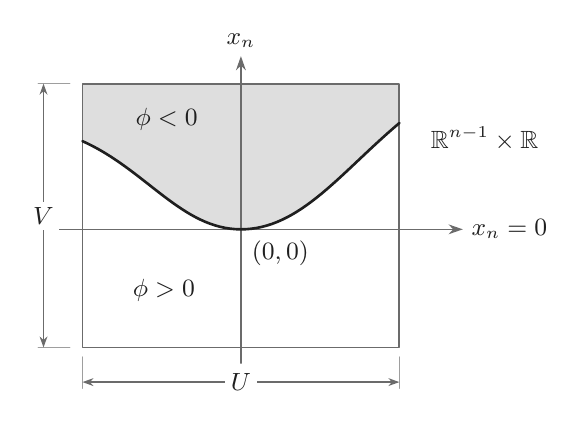
\begin{tikzpicture}[field/diagram, x=1.15cm, y=1.0cm]
    \def\LocalBoundary{
        (-1.75,1.12)
        .. controls (-1.05,0.76) and (-0.65,0) .. (0,0)
        .. controls (0.65,0) and (1.1,0.72) .. (1.75,1.35)
    }
    \fill[FieldRegion] \LocalBoundary
        -- (1.75,1.85) -- (-1.75,1.85) -- cycle;
    \draw[field/secondary] (-1.75,-1.50) rectangle (1.75,1.85);
    \draw[field/axis] (-2.15,0) -- (2.45,0)
        node[right] {$x_n=0$};
    \draw[field/axis] (0,-1.7) -- (0,2.2) node[above] {$x_n$};
    \draw[field/curve] \LocalBoundary;
    \node at (-0.82,1.40) {$\phi<0$};
    \node at (-0.85,-0.77) {$\phi>0$};
    \node[below right, inner sep=3pt] at (0,0) {$(0,0)$};
    \node[right] at (2.0,1.15) {$\mathbb R^{n-1}\times\mathbb R$};
    \draw[field/guide] (-1.89,-1.5) -- (-2.24,-1.5)
                       (-1.89,1.85) -- (-2.24,1.85);
    \draw[field/dimension] (-2.18,-1.5) -- (-2.18,1.85)
        node[midway, field/label] {$V$};
    \draw[field/guide] (-1.75,-1.62) -- (-1.75,-2.02)
                       (1.75,-1.62) -- (1.75,-2.02);
    \draw[field/dimension] (-1.75,-1.94) -- (1.75,-1.94)
        node[midway, field/label] {$U$};
\end{tikzpicture}

        \FieldCaption{I}{5}{}
    \end{minipage}
\end{center}
By the implicit function theorem we can choose an open neighbourhood $U\times V$ of $(0,0)\in\mathbb R^{n-1}\times\mathbb R$ such that $(U\times V)\cap\partial\Omega$ can be represented as the graph of a $C^2$ function $\psi:U\to V$. That is, $\phi(x,\psi(x))=0$, $x\in U$, and $(U\times V)\cap\partial\Omega=\{(x,\psi(x)):x\in U\}$.

Differentiating the identity $\phi(x,\psi(x))=0$ twice we obtain
\[0=D_1^2\phi_X+2D_{12}\phi_X.D\psi_x+D_2^2\phi_X.(D\psi_x,D\psi_x)+D_2\phi_X.D^2\psi_x,\quad x\in U.\]
Here we have set $X=(x,\psi(x))$ and we follow the derivative notation of Field \cite{bib:I:field-m-j:1}.

Now any tangent vector to $\operatorname{graph}(\psi)$ at $x$ is of the form $(v,D\psi_x(v))$, $v\in\mathbb R^{n-1}$. Set $V=(v,D\psi_x(v))$, $v\in\mathbb R^{n-1}$. Evaluating the above quadratic form on $V$, we obtain
\[0=H(\phi)(X)(V)+\frac{\partial\phi}{\partial x_n}(X)D^2\psi_x(v,v),\quad v\in\mathbb R^{n-1},\ x\in U.\]
Now $H(\phi)(X)(V)\geq0$ by assumption. Furthermore, since $\frac{\partial\phi}{\partial x_n}(0)<0$, we can find $s>0$ such that $\frac{\partial\phi}{\partial x_n}(X)<0$, $\|(x_1,\ldots,x_{n-1})\|<s$ ($\|\ \|$ denotes the Euclidean norm). Therefore, $D^2\psi_x(v,v)\geq0$, $\|x\|<s$, $v\in\mathbb R^{n-1}$.
% Original book page 76

Pick a unit vector $u\in\mathbb R^{n-1}$ and let $L_u$ denote the line through the origin of $\mathbb R^{n-1}$ defined by $u$. Let $\psi^u=\psi|L_u$. The positivity of $D^2\psi_x$ implies that
\[\frac{d^2\psi^u}{du^2}(x)\geq0,\quad x\in L^u,\ \|x\|<s.\]
As is well known this implies that the graph of $\psi^u$ is convex. In particular, $L^u\cap\operatorname{graph}(\psi^u)\neq\varnothing$. This is true for all unit vectors $u$ in $\mathbb R^{n-1}$ and so the open disc in $\mathbb R^{n-1}$ of radius $s$, centre 0, does not intersect $\Omega\cap\bar E_s(0)$. A straightforward argument based on the continuity of $\operatorname{grad}(\phi)$ shows that we can extend this result to find $r$, $0<r\leq s$, such that $T_y\partial\Omega\cap\bar E_r(0)\cap\Omega=\varnothing$, for all $y\in\partial\Omega\cap\bar E_r(0)$. As we pointed out above, this is sufficient to prove the convexivity of $\Omega$.
\end{proof}
\FieldHeading{Definition}{2.5.4}{}\FieldTarget{definition:2.5.4}{2.5.4} Let $\Omega$ be a proper subdomain of $\mathbb R^n$ with $C^2$ boundary. We say that $\Omega$ is \emph{strictly convex}\IndexMark{idx-139}{convexity@Convexity!strict@strict} if for some defining function $\phi$ for $\Omega$, $H(\phi)$ is positive definite on tangent vectors to $\partial\Omega$.
\FieldHeading{Proposition}{2.5.5}{}\FieldTarget{proposition:2.5.5}{2.5.5} Let $\Omega$ be a strictly convex bounded domain in $\mathbb R^n$ with $C^2$ boundary. Then there exists a defining function $\phi$ for $\Omega$ such that $H(\phi)(x)$ is a positive definite quadratic form for all $x\in\partial\Omega$.
\begin{proof}
Let $\theta$ be any $C^2$ defining function for $\Omega$. For $\lambda\in\mathbb R$, set $\phi_\lambda=\theta e^{\lambda\theta}$. Clearly for all values of $\lambda$, $\phi_\lambda$ is a $C^2$ defining function on $\Omega$ which is positive definite on tangent vectors to $\partial\Omega$. Computing the Hessian of $\phi_\lambda$ and restricting to $\partial\Omega$ we find
\[H(\phi_\lambda)(x)(v)=H(\theta)(x)(v)+2\lambda(d\theta(x)(v))^2,\quad v\in\mathbb R^n,\ x\in\partial\Omega.\]
Restrict $H(\phi_\lambda)$ to the compact set $\Gamma=\partial\Omega\times S^{n-1}$, where $S^{n-1}$ denotes the unit sphere in $\mathbb R^n$. Let $K=\{(x,u)\in\Gamma,\ d\theta(x)(v)=0\}$ (unit tangent bundle of $\partial\Omega$). $H(\theta)$ is strictly positive on $K$ and so, by continuity, is strictly positive on some open neighbourhood $U$ of $K$ in $\Gamma$. Let $m$ be the infimum of $2(d\theta(x)(v))^2$ over $\Gamma\setminus U$ and $M$ the supremum of $H(\theta)(x)(v)$ over $\Gamma\setminus U$. Since the compact set $\Gamma\setminus U$ does not meet the zero set of $d\theta$, $m>0$. Taking $\lambda_0=2M/m$, we see immediately that $H(\phi_\lambda)$ is strictly positive on $\Gamma$, $\lambda\geq\lambda_0$.
\end{proof}
% Original book page 77
This completes our review of convex domains in $\mathbb R^n$. Our aim is now to obtain a characterisation of domains of holomorphy with $C^2$ boundary in terms of local properties of the boundary. For the remainder of this section $\Omega$ will always denote an open, connected subset of $\mathbb C^n$.

We let $H_n(\mathbb C)$ denote the space of Hermitian quadratic forms on $\mathbb C^n$. Taking the standard complex basis on $\mathbb C^n$, we may identify $H_n(\mathbb C)$ with the space of $n\times n$ Hermitian matrices and we give $H_n(\mathbb C)$ the corresponding topology.
\FieldHeading{Definition}{2.5.6}{}\FieldTarget{definition:2.5.6}{2.5.6} Let $D$ be an open subset of $\mathbb C^n$, and $\phi\in C^2(D,\mathbb R)$. The \emph{Levi form}\IndexMark{idx-360}{levi form@Levi form} of $\phi$ is the map
\[L(\phi):D\to H_n(\mathbb C)\]
defined by
\[L(\phi)(z)=\left[\frac{\partial^2\phi}{\partial z_i\partial\bar z_j}\right],\quad z\in D.\]
\paragraph*{Remarks.}
\begin{enumerate}
\item Given $Z=(Z_1,\ldots,Z_n)\in\mathbb C^n$, $z\in D$,
\[L(\phi)(z)(Z)=\sum_{i,j=1}^n\frac{\partial^2\phi}{\partial z_i\partial\bar z_j}(z)Z_i\bar Z_j.\]
\item In Chapter~\ref{ch:5} we shall give an invariant definition of the Levi form.
\end{enumerate}
As we shall soon see the Levi form is the complex analogue of the Hessian.
\FieldHeading{Lemma}{2.5.7}{}\FieldTarget{lemma:2.5.7}{2.5.7} Let $\Omega,\Omega'$ be domains in $\mathbb C^n$ and $h:\Omega\to\Omega'$ be biholomorphic. If $\phi\in C^2(\Omega',\mathbb R)$ then
\[L(\phi h)=L(\phi)(Dh,\overline{Dh}).\]
(Here $[Dh]=[\partial h_i/\partial z_j]$; $[\overline{Dh}]=[\overline{\partial h_i/\partial z_j}]$).
\begin{proof}
We have to show that for $1\leq i,j\leq n$,
\[\frac{\partial^2\phi h}{\partial z_i\partial\bar z_j}=\sum_{\alpha,\beta=1}^n\frac{\partial^2\phi}{\partial z_\alpha\partial\bar z_\beta}\frac{\partial h_\alpha}{\partial z_i}\overline{\frac{\partial h_\beta}{\partial z_j}}.\]
This is a straightforward computation using Proposition~\ref{proposition:2.1.1} and we omit details.
\end{proof}
% Original book page 78
Lemma~\ref{lemma:2.5.7} shows that the Levi form is invariant under holomorphic changes of variables. Of course, the Hessian is only invariant under affine linear changes of variables.
\FieldHeading{Lemma}{2.5.8}{}\FieldTarget{lemma:2.5.8}{2.5.8} Let $\phi\in C^2(\Omega,\mathbb R)$. Then
\[L(\phi)=\tfrac14(H(\phi)+H(\phi)(J)).\]
That is, for $z\in\Omega$, $Z\in\mathbb C^n$,
\[L(\phi)(z)(Z)=\tfrac14(H(\phi)(z)(Z)+H(\phi)(z)(JZ)),\]
where on the right hand side we use the standard identification of $\mathbb C^n$ with $\mathbb R^{2n}$ and regard $Z\in\mathbb R^{2n}$ ($J$ denotes the standard complex structure on $\mathbb C^n$ (see \hyperref[sec:1:5]{\S5, Chapter 1})).
\begin{proof}
A straightforward, if tedious, calculation and we omit details.
\end{proof}
\paragraph*{Example 1.} Let $\Omega\subset\mathbb C^n$ be a bounded convex domain. We know from \hyperref[sec:2:4]{\S4} that every biholomorphic image of $\Omega$ is a domain of holomorphy. Suppose that $\Omega$ has $C^2$ boundary and that $g\in C^2(\bar\Omega,\mathbb C^n)$ is a diffeomorphism of some neighbourhood $U$ of $\bar\Omega$ into $\mathbb C^n$ which maps $\Omega$ biholomorphically onto a domain $\Omega'\subset\mathbb C^n$. Certainly $\Omega'$ has $C^2$ boundary and $\partial\Omega'=g(\partial\Omega)$. Set $h=(g|U)^{-1}$. If $\phi$ is a defining function for $\Omega$, then $\phi h$ is a defining function for $\Omega'$ ($\phi h$ is only defined on a neighbourhood of $\Omega'$, but we can always extend to a $C^2$ function on the whole of $\mathbb C^n$ which is strictly positive outside $\Omega'$). Since $\Omega$ is convex, $H(\phi)$ is positive semi-definite on tangent vectors to $\partial\Omega$. Suppose $Z$ is a holomorphic tangent vector to $\Omega'$ at $x$. That is,
\[\sum_{i=1}^n\frac{\partial(\phi h)}{\partial z_i}(x)Z_i=0,\quad Z=(Z_1,\ldots,Z_n).\]
Taking real and imaginary parts, we find that $Z$ and $JZ$ are \emph{real} tangent vectors to $\partial\Omega'$ at $x$. Therefore, by Lemmas~\ref{lemma:2.5.7}, \ref{lemma:2.5.8},
\[L(\phi h)(x)(Z)=\tfrac14\bigl(H(\phi)(x)(Dh_x(Z))+H(\phi)(x)(JDh_x(Z))\bigr)\geq0.\]
% Original book page 79
In other words, the Levi form is positive semi-definite on holomorphic tangent vectors to $\partial\Omega'$. Furthermore, if $\Omega$ is strictly convex, the Levi form will be positive definite on holomorphic tangent vectors to $\partial\Omega'$.
\paragraph*{Remark.} Of course a domain of holomorphy need not be the biholomorphic image of a convex set. However, if $\Omega$ is a domain in $\mathbb C^n$ with $C^2$ boundary and defining function $\phi$ such that $L(\phi)$ is positive definite at a point $z\in\partial\Omega$, then we may clearly make a local ($\mathbb C$-linear) holomorphic change of coordinates on some neighbourhood $U$ of $z$ such that, in the new coordinates, $U\cap\Omega$ is convex. In particular, if $L(\phi)$ is positive definite at all points of $\partial\Omega$, we see that $\Omega$ is locally the biholomorphic image of a convex set. Consequently, by example 1, $\Omega$ will locally be a domain of holomorphy. That is, for every $z\in\bar\Omega$, there will exist an open neighbourhood $U$ of $z$ in $\mathbb C^n$ such that $U\cap\Omega$ is a domain of holomorphy. However, if $L(\phi)$ is not positive definite and only positive semi-definite, even at just one point of $\partial\Omega$, it is not generally the case that $\Omega$ is locally the biholomorphic image of a convex set (it will however, be locally a domain of holomorphy). For examples and further references we refer the reader to the survey article by Y-T Siu \cite{bib:I:siu-y-t:1}, especially \S7. We should mention that the question of boundary invariants of domains with real analytic boundary is currently a topic of much interest. See, for example, the paper of Chern and Moser \cite{bib:I:chern-s-s-and-moser-j:1}.
\FieldHeading{Definition}{2.5.9}{}\FieldTarget{definition:2.5.9}{2.5.9} Let $\Omega$ be a domain in $\mathbb C^n$ with $C^2$ boundary. Suppose that there exists a defining function $\phi$ for $\Omega$ such that $L(\phi)$ is positive semi-definite on holomorphic tangent vectors to $\partial\Omega$. Then we say that $\Omega$ is \emph{Levi pseudoconvex}\IndexMark{idx-350}{l p domain@L.p. domain}\IndexMark{idx-362}{levi pseudoconvex@Levi pseudoconvex}\IndexMark{idx-480}{pseudoconvex@Pseudoconvex!levi@Levi} (abbreviated L.p.). In case $L(\phi)$ is positive definite on holomorphic tangent vectors to $\partial\Omega$, we say $\Omega$ is \emph{strictly Levi pseudoconvex}\IndexMark{idx-481}{pseudoconvex@Pseudoconvex!strictly levi@strictly Levi}\IndexMark{idx-535}{s l p domain@s.L.p. domain}\IndexMark{idx-586}{strictly levi pseudoconvex@Strictly Levi pseudoconvex} (abbreviated s.L.p.).

Exactly as we did for convex subsets of $\mathbb R^n$ we may prove
\FieldHeading{Lemma}{2.5.10}{}\FieldTarget{lemma:2.5.10}{2.5.10} Suppose $\Omega$ is a domain in $\mathbb C^n$ with $C^2$ boundary. If $\Omega$ is L.p. then $L(\phi)$ is positive semi-definite on holomorphic tangent vectors to $\partial\Omega$ for \emph{all} $C^2$ defining functions $\phi$ for $\Omega$. Similarly for s.L.p. domains.
\FieldHeading{Lemma}{2.5.11}{}\FieldTarget{lemma:2.5.11}{2.5.11} If $\Omega\subset\mathbb C^n$ is a bounded, strictly Levi pseudoconvex domain with $C^2$ boundary then there exists a defining function $\phi$ for such that $L(\phi)$ is positive definite on $\partial\Omega$.
% Original book page 80

Just as for convexivity, Levi\IndexMark{idx-366}{levi theorem@Levi theorem} pseudoconvexivity is a local property of the boundary. More precisely we have
\FieldHeading{Proposition}{2.5.12}{}\FieldTarget{proposition:2.5.12}{2.5.12} Let $\Omega$ be a bounded domain in $\mathbb C^n$ with $C^2$ boundary. Suppose that for each $x\in\partial\Omega$, there exists an open neighbourhood $U$ of $x$ and $\phi\in C^2(U,\mathbb R)$ such that
\begin{enumerate}
\item[a)] $\Omega\cap U=\{x\in U:\phi(x)<0\}$.
\item[b)] $d\phi\neq0$ on $\partial\Omega\cap U$.
\item[c)] $L(\phi)(y)(v)\geq0$ for all $y\in\partial\Omega\cap U$ and holomorphic tangent vectors $v$ to $\partial\Omega$ at $y$.
\end{enumerate}
Then $\Omega$ is Levi pseudoconvex. If in c), $L(\phi)$ is positive definite on holomorphic tangent vectors then $\Omega$ is strictly Levi pseudoconvex.
\begin{proof}
Since $\partial\Omega$ is compact, we can find finitely many open subsets $U_j$ of $\mathbb R^n$ and $\phi_j\in C^2(U_j,\mathbb R)$ such that $\partial\Omega\subset\bigcup U_j$ and the $\phi_j$ satisfy the conditions of the proposition. Set $U=\bigcup U_j$ and choose $\theta_i\in C_c^\infty(U_i)$ such that $\theta_i\geq0$ and $\bigcup_i\operatorname{Interior}(\operatorname{supp}(\theta_i))\supset\partial\Omega$. Define $\widetilde\phi=\sum\theta_i\phi_i\in C_c^\infty(U,\mathbb R)$. Since $\widetilde\phi(x)<0$ if $x\in\Omega\cap U$ and $\widetilde\phi(x)=0$ if $x\in\partial\Omega$, we may choose $\psi\in C^\infty(\mathbb C^n,\mathbb R)$ such that $\psi\equiv0$ on a neighbourhood of $\partial\Omega$ and $\Omega=\{x\in\mathbb C^n:(\widetilde\phi+\psi)(x)<0\}$, $\partial\Omega=\{x\in\mathbb C^n:(\widetilde\phi+\psi)(x)=0\}$. Set $\phi=\widetilde\phi+\psi$. On $\partial\Omega$,
\begin{align*}d\phi&=d\widetilde\phi=\sum\theta_i d\phi_i\\&\neq0.\end{align*}
Computing $L(\phi)$, we find that on $\partial\Omega$
\begin{align*}
L(\phi)(x)(v)&=\sum\theta_i(x)L(\phi_i)(x)(v),\quad\text{if }v\text{ is a holomorphic tangent vector to }\partial\Omega\text{ at }x,\\
&\geq0.
\end{align*}
\end{proof}
\FieldHeading{Theorem}{2.5.13}{ (E.E. Levi).}\FieldTarget{theorem:2.5.13}{2.5.13} Suppose $\Omega$ is a holomorphically convex domain in $\mathbb C^n$ with $C^2$ boundary. Then $\Omega$ is Levi pseudoconvex.
\begin{proof}
Let $\phi$ be a defining function for $\Omega$ and suppose that at some point $x\in\partial\Omega$, $L(\phi)$ is not positive semi-definite on holomorphic tangent vectors to $\partial\Omega$ at $x$. By a complex affine linear change of coordinates
% Original book page 81
we may suppose that $x=0$, $d\phi(0)=dx_1(0)$ and $L(\phi)(u)<0$, where $u$ is the unit basis vector in the $z_2$-direction. Thus, if for $1\leq i,j\leq n$ we set $\phi_i(0)=\frac{\partial\phi}{\partial z_i}(0)$, $\phi_{\bar j}(0)=\frac{\partial\phi}{\partial\bar z_j}(0)$, $\phi_{i\bar j}(0)=\frac{\partial^2\phi}{\partial z_i\partial\bar z_j}(0)$, etc., we will have
\[\phi_{\bar1}(0)=\phi_1(0)=\tfrac12;\quad\phi_i(0)=\phi_{\bar i}(0)=0,\ i>1;\quad\phi_{2\bar2}(0)<0.\]
For $t\in\mathbb R$, we define the analytic embedding $\phi_t:\mathbb C\to\mathbb C^n$ by
\[\phi_t(s)=(-2\phi_{22}(0)s^2-t,s,0,0,\ldots,0).\]
For $r>0$, set $V_t(r)=\phi_t(D_r(0))$. $V_t(r)$ is an embedded disc in $\mathbb C^n$. We observe that $0\in V_0(r)$. We claim that there exists $r>0$ such that
\[\overline{V_t(r)}\subset\Omega,\quad t\in(0,r]\]
\[\overline{V_0(r)}\setminus\{0\}\subset\Omega.\]
On the assumption that such an $r$ exists we now show that $\Omega$ cannot be holomorphically convex. Define
\[K=\bigcup_{0\leq t\leq r}\phi_t(\partial D_r(0))=\bigcup_{0\leq t\leq r}\partial V_t(r).\]
$K$ is a compact subset of $\Omega$. If $f\in A(\Omega)$, $0<t\leq r$, then $f\phi_t\in A(D_r(0))$ and is continuous on $\bar D_r(0)$. Hence, by the maximum principle, $\|f\phi_t\|_{\bar D_r(0)}=\|f\phi_t\|_{\partial D_r(0)}$. This implies that $\overline{V_t(r)}\subset\widehat K$, $0<t\leq r$. By continuity, $\overline{V_0(r)}\setminus\{0\}\subset\widehat K$. But therefore $\widehat K$ cannot be compact and so $\Omega$ is not holomorphically convex.

To construct $r$ we proceed as follows. By Taylor's theorem we may write
\[\phi(z)=x_1+\sum_{i,j}(\phi_{ij}(0)z_i z_j+\phi_{i\bar j}(0)z_i\bar z_j+\phi_{\bar i\bar j}(0)\bar z_i\bar z_j)+o(|z|^2).\]
Restricting $\phi$ to the sets $V_t$, we may regard $\phi$ as a function of $s$ and $t$. Substituting we find
\[\phi(s,t)=\phi_{2\bar2}(0)|s|^2+o(|s|^2)+tg(t,s),\]
% Original book page 82
where $g$ is a continuous function of $s$ and $t$ satisfying $g(0,0)=-1$. Since $\phi_{2\bar2}(0)<0$, we see that we can choose $r>0$ so that $\phi(s,t)<0$ for $t\in(0,r]$, $|s|\leq r$ or $t=0$, $0<|s|\leq r$.
\end{proof}
We may now state one of the most famous problems in several complex variables.
\paragraph*{Levi's problem (E.E. Levi \cite{bib:I:levi-e-e:1}).}\IndexMark{idx-364}{levi s problem@Levi's problem} Show that every Levi pseudoconvex domain in $\mathbb C^n$ is a domain of holomorphy.

Levi's problem was answered affirmatively by Oka \cite{bib:I:oka-k:1} in case $n=2$ and later, independently, by Bremermann \cite{bib:I:bremermann-h-j:1}, Norguet \cite{bib:I:norgeut-f:1} and Oka \cite{bib:I:oka-k:2} for general $n$. We shall give a proof of a generalisation of Levi's problem, due to Grauert, in Chapter~\ref{ch:7}.

For the remainder of this section we shall investigate some alternative pseudoconvexivity definitions. First we need a technical lemma, the proof of which was shown to us by D.B.A. Epstein.
\FieldHeading{Lemma}{2.5.14}{}\FieldTarget{lemma:2.5.14}{2.5.14} Let $\Omega$ be a bounded domain in $\mathbb R^n$ with $C^r$ boundary, $r\geq2$. Define $d:\mathbb R^n\to\mathbb R$ by
\[d(x)=\begin{cases}d(x,\partial\Omega),&x\in\Omega\\-d(x,\partial\Omega),&x\notin\Omega,\end{cases}\]
where distances are computed relative to the Euclidean metric on $\mathbb R^n$. Then $d$ is $C^r$ on some neighbourhood of $\partial\Omega$ in $\mathbb R^n$.
\begin{proof}
Let $n(z)$ denote the unit inward normal to $\partial\Omega$ at $z\in\partial\Omega$ and $\phi:\partial\Omega\times\mathbb R\to\mathbb R^n$ be the map $\phi(z,\lambda)=z+\lambda n(z)$. Thus $\phi$ is the exponential map of the normal bundle of $\partial\Omega$, relative to the Euclidean norm on $\mathbb R^n$. In particular, $\phi$ defines a $C^{r-1}$ diffeomorphism of some open neighbourhood of $\partial\Omega\times\{0\}\subset\partial\Omega\times\mathbb R$ onto an open neighbourhood $U$ of $\partial\Omega$ in $\mathbb R^n$ (note that $n(\ )$ is only of class $C^{r-1}$ on $\partial\Omega$). If $X\in U$ we may write $\phi^{-1}(X)=(\pi(X),\lambda(X))$, where $\pi:U\to\partial\Omega$, $\lambda:U\to\mathbb R$ are $C^{r-1}$ functions. Thus
\[X-\pi(X)=\lambda(X)n(\pi(X)),\quad X\in U.\]
% Original book page 83
Differentiating this expression with respect to $X$ and evaluating at $y\in\mathbb R^n$ we see that
\[y-D\pi_X(y)=D\lambda_X(y)n(\pi(X))+\lambda(X)Dn_{\pi(X)}(D\pi_X(y)).\]
Take the inner product with $n(\pi(X))$ to obtain
\[\langle y,n(\pi(X))\rangle=D\lambda_X(y)+\lambda(X)\langle Dn_{\pi(X)}(D\pi_X(y)),n(\pi(X))\rangle.\]
Now
\[\langle Dn_{\pi(X)}(D\pi_X(y)),n(\pi(X))\rangle=0\]
as is seen by differentiating the identity $\langle n(\pi(X)),n(\pi(X))\rangle=1$. Hence
\[D\lambda_X(y)=\langle y,n(\pi(X))\rangle.\]
But $\langle y,n(\pi(X))\rangle$ is a $C^{r-1}$ function of $X$. Therefore, $D\lambda$ is $C^{r-1}$ and so $\lambda$ is $C^r$. Since $d(x)=\lambda(x)$, the result follows.
\end{proof}
Continuing with the notation of the proof of Lemma~\ref{lemma:2.5.14}, we see that $Dd_x=\langle\cdot,n(\pi(x))\rangle$, for $x\in\partial\Omega$ and so $Dd$ is non-vanishing on $\partial\Omega$. Hence $-d$ is a continuous defining function for $\Omega$ which is $C^r$ on some neighbourhood of $\partial\Omega$ in $\mathbb R^n$.

Now suppose $\Omega$ is a bounded domain in $\mathbb C^n$ with $C^2$ boundary. As in Lemma~\ref{lemma:2.5.14}, we let $d:\mathbb C^n\to\mathbb R$ denote the signed Euclidean distance function to the boundary of $\Omega$.
\FieldHeading{Proposition}{2.5.15}{}\FieldTarget{proposition:2.5.15}{2.5.15} Let $\Omega$ be a bounded domain in $\mathbb C^n$ with $C^2$ boundary and suppose that $d:\mathbb C^n\to\mathbb R$ is $C^2$ on the open neighbourhood $U$ of $\partial\Omega$ in $\mathbb C^n$. Then the following conditions are equivalent:
\begin{enumerate}
\item[i)] $\Omega$ is Levi pseudoconvex.
\item[ii)] The Levi form of $-\log(d)$ is positive semi-definite on $U\cap\Omega$.
\end{enumerate}
\begin{proof}
First suppose that $L(-\log d)$ is positive semi-definite on $U\cap\Omega$. Set $\delta=-\log d=\log d^{-1}$. Computing we find that
\[\frac{\partial^2\delta}{\partial z_i\partial\bar z_j}=-d^{-1}\frac{\partial^2d}{\partial z_i\partial\bar z_j}+d^{-2}\frac{\partial d}{\partial z_i}\overline{\frac{\partial d}{\partial z_j}}\quad\text{on }U.\]
% Original book page 84
Hence for $z\in U\cap\Omega$, we have
\[\sum_{i,j}\frac{\partial^2d}{\partial z_i\partial\bar z_j}(z)Z_i\bar Z_j\geq0,\quad\text{provided that }\sum_i\frac{\partial d}{\partial z_i}(z)Z_i=0.\]
By continuity, this result holds on $\partial\Omega$ and so $\Omega$ is Levi pseudoconvex.

For the converse, we first note that since $-d$ is a $C^2$ defining function for $\Omega$, at least on $U$, Lemma~\ref{lemma:2.5.10} implies that $L(-d)$ is positive semi-definite on holomorphic tangent vectors to $\partial\Omega$. Suppose that there exists $z\in U\cap\Omega$ such that the Levi form of $-\log d$ is not positive semi-definite at $z$. This implies that there exists a unit vector $u\in\mathbb C^n$ such that
\[\left.\frac{\partial^2}{\partial t\partial\bar t}(\log d(z+tu))\right|_{t=0}>0.\]
As in the proof of Theorem~\ref{theorem:2.5.13}, Taylor's theorem implies that
\[\log d(z+tu)=\log d(z)+\operatorname{Re}(at+bt^2)+c|t|^2+O(|t|^2),\]
for constants $a,b\in\mathbb C$. Choose $\zeta\in\mathbb C^n$ such that $z+\zeta\in\partial\Omega$ and $d(z)=\|\zeta\|$. Consider the holomorphic curve
\[\phi(t)=z+tu+\zeta\exp(at+bt^2)\]
and note that $\phi(0)=z+\zeta\in\partial\Omega$. By the triangle inequality we have
\[d(\phi(t))\geq d(z+tu)-\|\zeta\|\exp(at+bt^2),\quad t\in\mathbb C.\]
Using the expression above for $\log d(z+tu)$ it follows that for sufficiently small values of $|t|$ we have
\[d(\phi(t))\geq\|\zeta\|(\exp(c|t|^2/2)-1)|\exp(at+bt^2)|.\]
But this estimate implies that at $t=0$ we have
\[\frac{\partial}{\partial t}d(\phi(t))=0\quad\text{and}\quad\frac{\partial^2}{\partial t\partial\bar t}d(\phi(t))>0\]
and so
% Original book page 85
\[\sum_i\frac{\partial d}{\partial z_i}(z+\zeta)\phi_i'(0)=0,\quad
\sum_{i,j}\frac{\partial^2d}{\partial z_i\partial\bar z_j}(z+\zeta)\phi_i'(0)\overline{\phi_j'(0)}<0,\]
contradicting the positive semi-definiteness of $L(d)$ on holomorphic tangent vectors to $\partial\Omega$.
\end{proof}
\FieldHeading{Definition}{2.5.16}{}\FieldTarget{definition:2.5.16}{2.5.16} Let $\Omega$ be a domain in $\mathbb C^n$ and $\phi:\Omega\to\mathbb R$ be $C^2$. We say that $\phi$ is \emph{plurisubharmonic}\IndexMark{idx-439}{plurisubharmonic@Plurisubharmonic}\IndexMark{idx-443}{plurisubharmonic@Plurisubharmonic!strict@strict} (psh for short) if $L(\phi)$ is positive semi-definite on $\Omega$. We say $\phi$ is \emph{strictly plurisubharmonic} if $L(\phi)$ is positive definite on $\partial$.
\paragraph*{Remark.} Notice that if $\phi:\Omega\to\mathbb R$ is $C^2$ and psh (respectively, strictly psh) and $h:\Omega'\to\Omega$ is biholomorphic then $h$ is psh (respectively, strictly psh).

In practice, it is useful to remove the differentiability requirement on psh functions. Thus suppose $\phi:\Omega\to[-\infty,+\infty)$ is semi-continuous from above. We say $\phi$ is psh if for arbitrary, $z,w\in\mathbb C^n$, the function $t\mapsto\phi(z+tw)$ is \emph{subharmonic} wherever defined. We recall that a function $u$ on a domain $U\subset\mathbb C$ is said to be subharmonic if given any compact subset $K$ of $U$ and continuous function $h$ on $K$ which is harmonic on $\mathring K$ and $\geq u$ on $\partial K$ then $u\leq h$ on $K$. Equivalently, $\phi$ is psh if $L(\phi)$ is positive semi-definite in the distributional sense. That is, if $\int_\Omega L(u)(x)(X)\phi(x)\,d\lambda(x)\geq0$ for all $u\in C_c^\infty(\Omega)$, $X\in\mathbb C^n$. We refer the reader to H\"ormander \cite{bib:I:hormander-l:1} or Vladimirov \cite{bib:I:vladimirov-v-s:1} for the basic properties of subharmonic and psh functions\IndexMark{idx-589}{subharmonic function@Subharmonic function} that are used in several complex variables. We should stress that the only reference to subharmonic functions in these notes will be in this section.

The next result is a generalisation of Proposition~\ref{proposition:2.5.15} to domains which do not have smooth boundary.
\FieldHeading{Proposition}{2.5.17}{}\FieldTarget{proposition:2.5.17}{2.5.17} If $\Omega$ is a domain of holomorphy in $\mathbb C^n$ then $-\log d(x)$ is psh.
\begin{proof}
See Bremermann \cite{bib:I:bremermann-h-j:2}, H\"ormander \cite{bib:I:hormander-l:1} or Vladimirov \cite{bib:I:vladimirov-v-s:1}.
\end{proof}
\FieldHeading{Definition}{2.5.18}{}\FieldTarget{definition:2.5.18}{2.5.18} A domain $\Omega$ in $\mathbb C^n$ is said to be \emph{pseudoconvex}\IndexMark{idx-478}{pseudoconvex@Pseudoconvex} if $-\log d(x)$ is psh.

We now define a very strong form of pseudoconvexivity.
% Original book page 86
\FieldHeading{Definition}{2.5.19}{}\FieldTarget{definition:2.5.19}{2.5.19} A domain $\Omega$ in $\mathbb C^n$ is said to be \emph{0-complete}\IndexMark{idx-660}{zero complete 0 complete@Zero-complete (0-complete)} or \emph{holomorphically complete}\IndexMark{idx-306}{holomorphically complete@Holomorphically complete} if there exists $\phi\in C_{\mathbb R}^\infty(\Omega)$ such that
\begin{enumerate}
\item $\phi$ is strictly psh.
\item For every $a\in\mathbb R$, $\Omega_a=\{z\in\Omega:\phi(z)<a\}$ is relatively compact in $\Omega$.
\end{enumerate}
It is not hard to show that a domain $\Omega$ in $\mathbb C^n$ is pseudoconvex if and only if it is 0-complete. See, for example, H\"ormander \cite{bib:I:hormander-l:1} or Vladimirov \cite{bib:I:vladimirov-v-s:1}. We shall prove directly that every domain of holomorphy is 0-complete.
\FieldHeading{Theorem}{2.5.20}{}\FieldTarget{theorem:2.5.20}{2.5.20} Let $\Omega$ be a domain of holomorphy. Then $\Omega$ is 0-complete.
\begin{proof}
Since $\Omega$ is holomorphically convex we may find a normal exhaustion\IndexMark{idx-243}{exhaustion function@Exhaustion function} $(K_n)_{n\geq1}$ of $\Omega$. Choose an increasing sequence $(U_n)$ of relatively compact open subsets of $\Omega$ such that for all $n$, $K_n\subset U_n$ and $U_n$ is relatively compact in $U_{n+1}$. Since $\widehat K_n=K_n$ and $\bar U_{n+1}\setminus U_n$ is compact there exist $f_{nk}\in A(\Omega)$, $1=1,\ldots,k(n)$, such that
\[\|f_{nk}\|_{K_n}<1\quad\text{and}\quad\max_k|f_{nk}(z)|>1,\quad z\in\bar U_{n+1}\setminus U_n.\]
Raising the $f_{nk}$ to sufficiently high powers we may further assume that
\[\sum_{n=1}^{k(n)}|f_{nk}(z)|^2<2^{-n},\quad z\in K_n.\tag{A}\label{eq:2:a:1}\]
\[\sum_{k=1}^{k(n)}|f_{nk}(z)|^2>n,\quad z\in\bar U_{n+1}\setminus U_n.\tag{B}\label{eq:2:b:1}\]
Since $\Omega\subset\mathbb C^n$, we may further require that for every $z\in K_n$ there exist $n$ of the $f_{nk}$ which gives local holomorphic coordinates at $z$. Define
\[\phi(z)=\sum_{n,k}|f_{nk}(z)|^2,\quad z\in\Omega.\]
The sum converges by estimate A for all $z\in\Omega$. We claim that $\phi\in C_{\mathbb R}^\infty(\Omega)$. This follows since $\sum f_{nk}(z)\overline{f_{nk}(\zeta)}$ is uniformly convergent on compact subsets of $\Omega\times\Omega$ and so, by Corollary~\ref{corollary:2.1.8}, the sum is analytic in $z$ and $\bar\zeta$. Next notice that estimate B implies that $\phi(z)>n$, for $z\in\Omega\setminus U_n$. Hence, for all $a\in\mathbb R$, $\Omega_a=\{z:\phi(z)<a\}$ is relatively compact. Finally, we have
% Original book page 87
\[L(\phi)=\sum\frac{\partial f_{nk}}{\partial z_i}\overline{\frac{\partial f_{nk}}{\partial z_j}}\]
and so $L(\phi)$ is certainly positive semi-definite. To prove positive definiteness suppose that $L(\phi)(z)(Z)=0$, $z\in K_n$. This implies that $\sum_{i,k}\frac{\partial f_{nk}}{\partial z_i}(z)Z_i=0$. But it is possible to find $n$ of the $f_{nk}$ which give a local coordinate system at $z$. Hence $Z=0$.
\end{proof}
\paragraph*{Remarks.}
\begin{enumerate}
\item We call functions $\phi$ that satisfy the conditions of Definition~\ref{definition:2.5.19} \emph{strictly psh exhaustion functions}\IndexMark{idx-441}{plurisubharmonic@Plurisubharmonic!exhaustion function@exhaustion function} for $\Omega$. Notice that our definition of 0-completeness is invariant under biholomorphic maps and makes no explicit mention of the boundary of $\Omega$. Later, in Chapter~\ref{ch:5}, we shall generalise our 0-completeness definition to complex manifolds.
\item It follows easily from Sard's theorem that if $\Omega$ is 0-complete then $\Omega$ is the limit of an increasing sequence of s.L.p. domains (see also the discussion in \hyperref[sec:7:4]{\S4, Chapter 7}).
\end{enumerate}
Next we wish to give a brief discussion of some ``continuity'' principles that hold for pseudoconvex\IndexMark{idx-479}{pseudoconvex@Pseudoconvex!h@H-} domains. Motivation for the next definition is given by the proof of Theorem~\ref{theorem:2.5.13}.
\FieldHeading{Definition}{2.5.21}{}\FieldTarget{definition:2.5.21}{2.5.21} A domain $\Omega$ in $\mathbb C^n$ is said to satisfy the \emph{weak continuity principle}\IndexMark{idx-647}{weak continuity principle@Weak continuity principle} if, given any sequence $\{V_n\}$ of holomorphically embedded discs in $\Omega$ which satisfy
\begin{enumerate}
\item For all $n$, $V_n\cup\partial V_n$ is a relatively compact subset of $\Omega$.
\item $\lim V_n=V_0$ exists and $\partial V_0$ is relatively compact subset of $\Omega$.
\end{enumerate}
Then, provided that $V_0$ is bounded, $V_0$ is a relatively compact subset of $\Omega$.

Using subharmonic functions it is not too hard to show that a domain is pseudoconvex if and only if it satisfies the weak continuity principle (see Bremermann \cite{bib:I:bremermann-h-j:2}, Vladimirov \cite{bib:I:vladimirov-v-s:1}). If we say that a domain $\Omega$ in $\mathbb C^n$ is H-pseudoconvex\IndexMark{idx-279}{h pseudoconvex@H-pseudoconvex} if it contains all its generalised Hartogs figures, then it is straightforward to show that $\Omega$ is H-pseudoconvex if and only if it satisfies the weak continuity principle (see Grauert and Fritzsche \cite{bib:I:grauert-h-and-fritzche-k:1} and also Andreotti and Grauert \cite[page 217ff]{bib:I:andreotti-a-and-grauert-h:1}).
% Original book page 88

Let us summarise the relations between the various definitions we have been considering.
\begin{center}
    \begin{minipage}{\linewidth}
        \centering
        % The arrow directions are exactly those in the source diagram.
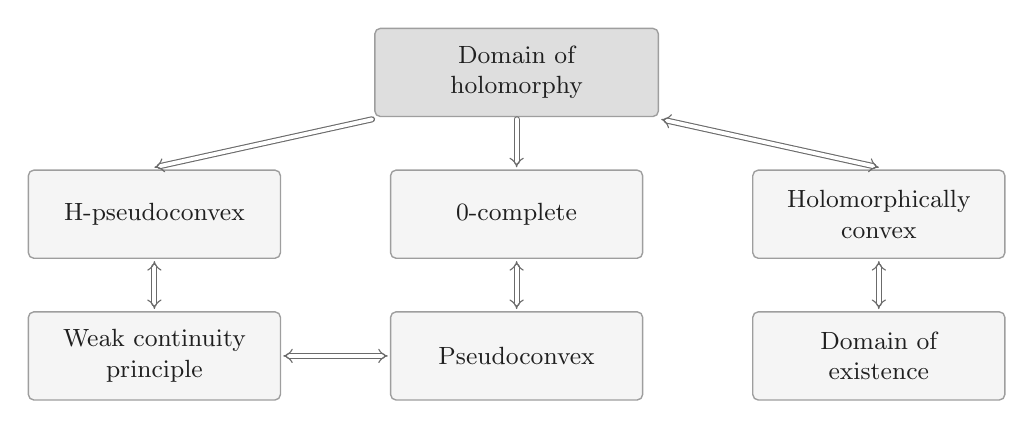
\begin{tikzpicture}[field/diagram]
    \node[field/concept, text width=3.25cm, fill=FieldRegion]
        (dh) at (0,2.85) {Domain of holomorphy};
    \node[field/concept] (hp) at (-4.6,1.05) {H-pseudoconvex};
    \node[field/concept] (oc) at (0,1.05) {0-complete};
    \node[field/concept] (hc) at (4.6,1.05) {Holomorphically\\convex};
    \node[field/concept] (wc) at (-4.6,-0.75) {Weak continuity\\principle};
    \node[field/concept] (pc) at (0,-0.75) {Pseudoconvex};
    \node[field/concept] (de) at (4.6,-0.75) {Domain of existence};
    \draw[field/implies] (dh.south west) -- (hp.north);
    \draw[field/implies] (dh.south) -- (oc.north);
    \draw[field/equivalent] (dh.south east) -- (hc.north);
    \draw[field/equivalent] (hp.south) -- (wc.north);
    \draw[field/equivalent] (oc.south) -- (pc.north);
    \draw[field/equivalent] (hc.south) -- (de.north);
    \draw[field/equivalent] (wc.east) -- (pc.west);
\end{tikzpicture}

    \end{minipage}
\end{center}
In Chapter 12 we shall prove the fundamental result that every 0-complete domain in $\mathbb C^n$ is a domain of holomorphy. As a consequence, the definitions above will have all been shown to be equivalent.

Finally the reader interested in pseudoconvexivity and its relationship with domains of holomorphy should certainly consult the original works of Oka \cite{bib:I:oka-k:3} and the H. Cartan seminar [2].
\paragraph*{Exercises.}
\begin{enumerate}
\item Show that Lemma~\ref{lemma:2.5.10} is false if $\partial\Omega$ is only $C^1$. Can you find an example of a domain in $\mathbb C^n$ with $C^1$ boundary such that $d(x)$ is not differentiable at any point of $\mathbb C^n$?
\item Show
\begin{enumerate}
\item[a)] The interior of an arbitrary intersection of pseudoconvex domains is pseudoconvex (cf. Example 15, \hyperref[sec:2:4]{\S4}).
\item[b)] If $\Omega$ is a domain in $\mathbb C^n$ such that every point $z\in\partial\Omega$ has an open neighbourhood $U$ such that $U\cap\Omega$ is pseudoconvex then $\Omega$ is pseudoconvex (the same result is true for domains of holomorphy but depends on the equivalence between domains of holomorphy and pseudoconvex domains).
\end{enumerate}
(Both a) and b) use elementary properties of subharmonic functions).
\item (Kohn and Nirenberg \cite{bib:I:kohn-j-j-and-nirenberg-l:1}). Show that the domain $\Omega$ in $\mathbb C^2$ defined by $\operatorname{Re}(w)+|zw|^2+|z|^8+\frac{15}{7}|z|^2\operatorname{Re}(z^6)<0$ is L.p. and s.L.p. at every point of $\partial\Omega$ except 0.
% Original book page 89

($\Omega$ is not convex at 0 in any local system of holomorphic coordinates, See Kohn and Nirenberg \cite{bib:I:kohn-j-j-and-nirenberg-l:1} and also Y.T. Siu \cite{bib:I:siu-y-t:1}).
\end{enumerate}

\section{The Bergman kernel function}\IndexMark{idx-038}{bergman kernel function@Bergman kernel function}\label{sec:2:6}
In this section we describe how some domains of holomorphy in $\mathbb C^n$ have an intrinsic strictly psh exhaustion function (granted the Euclidean metric structure on $\mathbb C^n$). For the most part we either omit or give very brief indications of proofs. Full details may be found in Bergman \cite{bib:I:bergman-s:1,bib:I:bergman-s:2} or Fuks \cite{bib:I:fuks-b-a:1}. We shall also assume some elementary Hilbert space theory.

Throughout this section we shall suppose that $\Omega$ is a bounded domain in $\mathbb C^n$. We have already shown in Exercise 2, \hyperref[sec:2:1]{\S1}, that $L^2(\Omega)$ is a Hilbert space with inner product defined by $(f,g)=\int_\Omega\bar f g\,d\lambda$, where $d\lambda$ is Lebesgue measure on $\mathbb C^n$. We set $|f|=(f,f)^{\frac12}$, $f\in L^2(\Omega)$. Since $L^2(\Omega)$ is separable, we may find a countable orthonormal (Hilbert space) basis $\{\phi_j:j\geq1\}$ for $L^2(\Omega)$. We remark that if $\{\psi_j\}$ is an arbitrary Hilbert space basis for $L^2(\Omega)$ then we can construct an orthonormal basis for $L^2(\Omega)$ from $\{\psi_j\}$ using the Gram--Schmidt orthogonalisation process.
\FieldHeading{Proposition}{2.6.1}{}\FieldTarget{proposition:2.6.1}{2.6.1} Let $\{\phi_j\}$ be an orthonormal basis for $L^2(\Omega)$. Given $f\in L^2(\Omega)$, set $a_j=(\phi_j,f)$, $j\geq1$. Then
\begin{enumerate}
\item $f=\sum_{j=1}^\infty a_j\phi_j$, where convergence is uniform on compact subsets of $\partial\Omega$.
\item $|f|^2=\sum_{j=1}^\infty|a_j|^2$ (Parseval's equality).
\end{enumerate}
\begin{proof}
Straightforward and based on the estimates of Exercise 2, \hyperref[sec:2:1]{\S1}. See also the proof of Proposition~\ref{proposition:2.6.2} below.
\end{proof}
\FieldHeading{Proposition}{2.6.2}{}\FieldTarget{proposition:2.6.2}{2.6.2} Let $\{\phi_j\}$ be an orthonormal basis for $L^2(\Omega)$. Then the series
\[\sum_{j=1}^\infty\phi_j(z)\overline{\phi_j(\zeta)}\]
converges uniformly on compact subsets of $\Omega\times\Omega$ to a function $K_\Omega(z,\bar\zeta)$ which is analytic in $(z,\bar\zeta)$. In particular, $K_\Omega$ is $C^\infty$.
% Original book page 90
\begin{proof}
Let $D_0=D(z_0;r)$, $D_1=D(\zeta_0;s)$ be relatively compact polydiscs in $\Omega$. By Exercise 2, \hyperref[sec:2:1]{\S1}, there exists $C_0\geq0$ such that for all $f\in L^2(\Omega)$, $\|f\|_{\bar D_0}\leq C_0|f|$. Therefore for $z\in D_0$ we have
\begin{align*}
\sum_{j=1}^m|\phi_j(z)|^2&=\int_\Omega\left|\sum_{j=1}^m\phi_j(\tau)\overline{\phi_j(z)}\right|^2\,d\lambda(\tau)\\
&\geq C_0\left\|\sum_{j=1}^m\phi_j(\tau)\overline{\phi_j(z)}\right\|_{D_0}^2\\
&\geq C_0\left\|\sum_{j=1}^m|\phi_j(z)|^2\right\|_{D_0}^2.
\end{align*}
Hence
\[\sum_{j=1}^m|\phi_j(z)|^2\leq C_0^{-1},\quad z\in D_0.\]
Similarly,
\[\sum_{j=1}^m|\phi_j(\zeta)|^2\leq C_1^{-1},\quad\zeta\in D_1.\]
By the Cauchy--Schwarz inequality
\[\left\{\sum_{j=1}^m|\phi_j(z)\overline{\phi_j(\zeta)}|\right\}^2\leq\left\{\sum_{j=1}^m|\phi_j(z)|^2\right\}^2\left\{\sum_{j=1}^m|\phi_j(\zeta)|^2\right\}^2\]
and so
\[\sum_{j=1}^m|\phi_j(z)\overline{\phi_j(\zeta)}|\leq(C_0C_1)^{-1},\quad z\in D_0,\ \zeta\in D_1.\]
Therefore $\sum_{j=1}^\infty\phi_j(z)\overline{\phi_j(\zeta)}$ converges uniformly on compact subsets of $\Omega\times\Omega$ and so the result follows by Corollary~\ref{corollary:2.1.8}.
\end{proof}
\FieldHeading{Definition}{2.6.3}{}\FieldTarget{definition:2.6.3}{2.6.3} Let $\{\phi_j\}$ be an orthonormal basis for $L^2(\Omega)$. Then the function $K_\Omega(z,\bar\zeta)=\sum_{j=1}^\infty\phi_j(z)\overline{\phi_j(\zeta)}$ is called the \emph{(Bergman) kernel function} of the domain $\Omega$, relative to the orthonormal basis $\{\phi_j\}$.
\FieldHeading{Theorem}{2.6.4}{}\FieldTarget{theorem:2.6.4}{2.6.4} The kernel function $K_\Omega(z,\bar\zeta)$ is independent of the choice of orthonormal basis for $L^2(\Omega)$. It satisfies the following characteristic variational property:
% Original book page 91
Given $z_0\in\Omega$, the function
\[f(z)=K_\Omega(z,\bar z_0)/K_\Omega(z_0,\bar z_0)\]
is the unique function in $L^2(\Omega)$ which minimises the integral $|f|$, subject to the normalising condition $f(z_0)=1$.
\begin{proof}
Straightforward and we refer to the references.
\end{proof}
In view of Theorem~\ref{theorem:2.6.4} we may now talk about \emph{the} kernel function of the domain $\Omega$.
\FieldHeading{Theorem}{2.6.5}{ (Reproducing property of the kernel function).}\IndexMark{idx-507}{reproducing property of kernel function@Reproducing property of kernel function}\FieldTarget{theorem:2.6.5}{2.6.5} For all $f\in L^2(\Omega)$, we have
\[f(z)=\int_\Omega f(\zeta)K_\Omega(z,\bar\zeta)\,d\lambda(\zeta).\]
\begin{proof}
Take the Fourier series expansion of $f$ relative to an orthonormal basis of $L^2(\Omega)$ and integrate term by term.
\end{proof}
\paragraph*{Example.} Set $D=D(0;r_1,\ldots,r_n)$, $E=E(0;r)$. Then $\{z^m/m!:m\in\mathbb N^n\}$ is easily seen to be an orthogonal basis for both $L^2(D)$ and $L^2(E)$. Normalising and computing the kernel functions we find
\[K_D(z,\bar\zeta)=\pi^{-n}r_1^2\cdots r_n^2\prod_{j=1}^n(r_j-z_j\bar\zeta_j)^{-2}\]\IndexMark{idx-039}{bergman kernel function@Bergman kernel function!of polydisc@of polydisc}
\[K_E(z,\bar\zeta)=\pi^{-n}r^2n!\left(r^2-\sum_{j=1}^n z_j\bar\zeta_j\right)^{-n-1}.\]\IndexMark{idx-040}{bergman kernel function@Bergman kernel function!of euclidean disc@of Euclidean disc}
Observe that $K_D(z,\bar z)$, $K_E(z,\bar z)$ are strictly psh exhaustion functions for their respective domains. The reader may find computations of the kernel functions of the ``classical domains'' (see \hyperref[sec:4:2]{Chapter 4, \S2}) in Hua \cite{bib:I:hua-l-k:1}.

Next we examine how the kernel function transforms under biholomorphic maps.
\FieldHeading{Proposition}{2.6.6}{}\FieldTarget{proposition:2.6.6}{2.6.6} Let $h:\Omega\to\Omega'$ be a biholomorphic map between bounded domains in $\mathbb C^n$. Then
\[K_\Omega(z,\bar z)=K_{\Omega'}(h(z),\overline{h(z)})|\det_{\mathbb C}Dh_z|^2.\]
% Original book page 92
\begin{proof}
A straightforward computation using the change of variables formula for multiple integrals and the fact that $\det_{\mathbb R}Dh_z=|\det_{\mathbb C}Dh_z|^2$ (see \hyperref[sec:5:4]{\S4, Chapter 5}).
\end{proof}
\paragraph*{Remarks.}
\begin{enumerate}
\item Proposition~\ref{proposition:2.6.6} implies that the kernel function is invariantly defined as a section of an appropriate tensor bundle on $\Omega$. We return to this point in Chapter~\ref{ch:5}.
\setcounter{enumi}{2}
\item Note that Proposition~\ref{proposition:2.6.6} in combination with the computations of the Example, shows that the open polydisc and Euclidean disc in $\mathbb C^n$ are biholomorphically inequivalent\IndexMark{idx-046}{biholomorphic inequivalence of disc and polydisc@Biholomorphic inequivalence of disc and polydisc}, $n>1$. See also \hyperref[sec:4:2]{\S2 of Chapter 4}.
\end{enumerate}
\FieldHeading{Corollary}{2.6.7}{}\FieldTarget{corollary:2.6.7}{2.6.7} The Levi form of\IndexMark{idx-041}{bergman kernel function@Bergman kernel function!levi form of@Levi form of} $\log K_\Omega(z,\bar z)$ is invariant under biholomorphic transformations.

Because of Corollary~\ref{corollary:2.6.7} and the analogy with pseudoconvexivity we prefer to work with $\log K_\Omega(z,\bar z)$ rather than $K_\Omega(z,\bar z)$.
\FieldHeading{Proposition}{2.6.8}{}\FieldTarget{proposition:2.6.8}{2.6.8} Let $\Omega$ be a bounded domain in $\mathbb C^n$. Then $\log K_\Omega(z,\bar z)$ is a $C^\infty$ strictly psh function.
\begin{proof}
A straightforward computation that makes use of the fact that since $\Omega$ is bounded we can define local coordinate systems at any point of $\Omega$ using elements of a fixed orthonormal basis for $L^2(\Omega)$.
\end{proof}
The question now arises as to the conditions under which $\log K_\Omega(z,\bar z)$ gives a strictly psh exhaustion function for a domain of holomorphy $\Omega$. In general it does not (see Bremermann \cite{bib:I:bremermann-h-j:3}). However, it is certainly true that a sufficient condition for $\Omega$ to be a domain of holomorphy is that $\log K_\Omega(z,\bar z)$ is a strictly psh exhaustion function for $\Omega$. Moreover, it can be shown that every domain of holomorphy is the limit of an increasing sequence of domains of holomorphy for which $\log K(z,\bar z)$ is a strictly psh exhaustion function (see Bremermann \cite{bib:I:bremermann-h-j:2} and compare with the corresponding approximation of domains of holomorphy by s.L.p. domains). Finally we should mention that if we define a weighted inner product $(f,g)_\phi=\int_\Omega\bar f g e^{-\phi}\,d\lambda$ and let $L^2(\Omega;\phi)$ denote the corresponding Hilbert space of analytic functions on $\Omega$, then the kernel theory continues to hold. Sharp estimates on the growth of the associated kernel function at the boundary of $\Omega$ are given in H\"ormander \cite{bib:I:hormander-l:3}. See also Bremermann \cite{bib:I:bremermann-h-j:2}. Notice that the introduction of weighting functions amounts to a change of metric on $\Omega$.
% Original book page 93

For a survey of recent results on the kernel function and its applications to complex analysis see Diederich \cite{bib:I:diederich-k:1}.
\paragraph*{Exercises.}
\begin{enumerate}
\item Verify that the kernel function of a domain $\Omega$ is Hermitian: $K_\Omega(z,\zeta)=\overline{K_\Omega(\zeta,z)}$, $z,\zeta\in\Omega$.
\item Verify the expressions for the kernel functions of the polydisc and Euclidean disc given in the example.
\end{enumerate}

\section{The Cousin problems}\IndexMark{idx-144}{cousin domains@Cousin domains}\IndexMark{idx-148}{cousin problems@Cousin problems}\label{sec:2:7}
In this section we wish to consider the problem of constructing meromorphic functions with specified principle parts or zero and pole sets on a given domain in $\mathbb C^n$, $n>1$. These questions were first raised by P. Cousin around the turn of the century and, following H. Cartan \cite{bib:I:cartan-h:1}, now bear his name. As yet, of course, we have not defined meromorphic functions of more than one variable (see Chapter~\ref{ch:3}) but, as we showed in Chapter~\ref{ch:1}, it is possible to formulate both the Mittag--Leffler and Weierstrass theorems in a way that avoids explicit mention of meromorphic functions. We adopt this approach here but we must caution the reader that our consequent definition of the Cousin problems is \emph{not} the classical one (see the remarks below).
\paragraph*{Cousin's problem A.}
Let $\Omega$ be a domain in $\mathbb C^n$ and $\{U_i:i\in I\}$ be an open cover of $\Omega$. Suppose we are given $f_{ij}\in A(U_{ij})$ such that for all $i,j,k$
\[f_{ij}=-f_{ji}\text{ on }U_{ij};\quad f_{ij}+f_{jk}+f_{ki}=0\text{ on }U_{ijk}.\]
When can we find $f_i\in A(U_i)$ such that $f_{ij}=f_j-f_i$ on $U_{ij}$ for all $i,j\in I$?

We say $\Omega$ is a \emph{Cousin A domain} if we can always solve the Cousin A problem on $\Omega$.
\paragraph*{Cousin's problem B.}
Let $\Omega$ be a domain in $\mathbb C^n$ and $\{U_i:i\in I\}$ be an open cover of $\Omega$. Suppose we are given $f_{ij}\in A^*(U_{ij})$ such that for all $i,j,k$
% Original book page 94
\[f_{ij}=f_{ji}^{-1}\text{ on }U_{ij};\quad f_{ij}f_{jk}f_{ki}=1\text{ on }U_{ijk}.\]
When can we find $f_i\in A(U_i)$ such that $f_{ij}=f_j/f_i$ on $U_{ij}$ for all $i,j\in I$?

We say $\Omega$ is a \emph{Cousin B domain}\IndexMark{idx-145}{cousin domains@Cousin domains} if we can always solve the Cousin B problem\IndexMark{idx-149}{cousin problems@Cousin problems} on $\Omega$.
\FieldHeading{Proposition}{2.7.1}{}\FieldTarget{proposition:2.7.1}{2.7.1} Let $\Omega$ be a domain in $\mathbb C^n$. Then
\begin{enumerate}
\item $\Omega$ is a Cousin A domain if and only if we can solve the Cauchy--Riemann equations on $\Omega$.
\item $\Omega$ is a Cousin B domain if and only if every holomorphic line bundle on $\Omega$ is holomorphically trivial.
\end{enumerate}
\begin{proof}
To say that we can solve the Cauchy--Riemann equations on $\Omega$ means that if we are given $f_j\in C^\infty(\Omega)$, $1\leq j\leq n$, such that $\partial f_j/\partial\bar z_i=\partial f_i/\partial\bar z_j$, $1\leq i,j\leq n$, then there exists $u\in C^\infty(\Omega)$ such that $\partial u/\partial\bar z_j=f_j$, $1\leq j\leq n$ (see \hyperref[sec:2:3]{\S3}, especially Theorem~\ref{theorem:2.3.1}). Suppose that we can solve the Cauchy--Riemann equations on $\Omega$. Then, exactly as in the proof of Theorem~\ref{theorem:1.3.2}, we can solve the Cousin A problem on $\Omega$. We defer the proof of the converse to Chapter~\ref{ch:6}. The second statement is an immediate consequence of the definition of a holomorphically trivial line bundle (see \hyperref[sec:1:5]{\S5, Chapter 1}).
\end{proof}
We know from Chapter~\ref{ch:1} that every domain in $\mathbb C$ is a Cousin A and Cousin B domain. Notice that if $\Omega$ is a domain in $\mathbb C$ and $f_{ij}\in A(U_{ij})$ is the data for a Cousin A problem on $\Omega$ then we can find $m_j\in M(U_j)$ such that $f_{ij}=m_j-m_i$. Indeed, we can choose $m_j\in A(U_j)$ satisfying these conditions since $\Omega$ is a Cousin A domain! Hence, for domains in $\mathbb C$, there is really no difference between the Cousin A problem and the problem of constructing meromorphic functions with specified principal parts. Similarly for the multiplicative problem. It turns out that this equivalence between the Cousin A and B problems and the problem of finding meromorphic functions with specified principal parts or pole and zero sets no longer holds for domains in $\mathbb C^n$, $n>1$. As we shall see in Chapter 12, it is possible, for example, to have domains in $\mathbb C^2$ for which we can always construct meromorphic functions with specified pole and zero sets but which are nevertheless not Cousin B (or A) domains. To clarify this point we now give the original definition of a Cousin II domain.
% Original book page 95
\FieldHeading{Definition}{2.7.2}{}\FieldTarget{definition:2.7.2}{2.7.2} We say that a domain $\Omega$ in $\mathbb C^n$ is a \emph{Cousin II domain} if given any open cover $\{U_i\}$ of $\Omega$ and analytic functions $f_i\in A^*(U_i)$ such that $f_i/f_j\in A^*(U_{ij})$ then there exists $F\in A(\Omega)$ such that $Ff_i^{-1}\in A^*(U_i)$ for all $i$.
\paragraph*{Remark.} We shall see in \hyperref[sec:3:4]{\S4 of Chapter 3}, if $\Omega$ is a Cousin II domain then we can construct meromorphic functions on $\Omega$ with specified pole and zero sets. However, a Cousin II domain need not be a Cousin B domain if $n>1$.
\paragraph*{Examples.}
\begin{enumerate}
\item Every open polydisc $D\subset\mathbb C^n$ is a Cousin A domain. To prove this we shall show that the Cauchy--Riemann equations are solvable in $D$. Our proof will be very close to that of Theorem~\ref{theorem:1.3.1}. Let $D=D(0;r_1,\ldots,r_n)$ and for $s\in(0,1]$, set $D_s=sD$. Suppose $f\in A(D)$. By Theorem~\ref{theorem:2.1.5}
\[f(z)=\sum\frac1{m!}\partial^m f(0)z^m,\quad z\in D,\]
with uniform convergence on compact subsets of $D$. Hence, given $s\in(0,1)$ and $\epsilon>0$, there exists $N>0$ such that $\|f-f_N\|_{\bar D_s}\leq\epsilon$, where $f_N(z)=\sum_{|m|\leq N}\frac{\partial^m f(0)}{m!}z^m$. Hence polynomials are dense in $A(D)$. Using this approximation result together with Theorem~\ref{theorem:2.3.1} we can now use the method of proof of Theorem~\ref{theorem:A1.8} (Theorem~\ref{theorem:1.3.1}) to show that the Cauchy--Riemann equations are solvable on $D$. We leave details to the reader (see also Theorem~\ref{theorem:5.8.2}).

This example can be generalised in the following way: We say that $\Omega\subset\mathbb C^n$ is a \emph{Runge domain}\IndexMark{idx-533}{runge domain@Runge domain} if polynomials are dense in $A(\Omega)$. It may be proved, using an ingenious inductive argument due to Oka, that the Cauchy--Riemann equations may always be solved on a Runge domain. For further details and references we refer the reader to H\"ormander \cite{bib:I:hormander-l:1}, Gunning and Rossi \cite{bib:I:gunning-r-c-and-rossi-h:1}.
\item The domain $\Omega=\mathbb C^2\setminus\{0\}$ is not a Cousin A domain. We shall show that the Cauchy--Riemann equations are not always solvable on $\Omega$. Let $z=(z_1,z_2)\in\Omega$ and set $\|z\|^2=|z_1|^2+|z_2|^2$. We define functions $f_1,f_2$ by
% Original book page 96
\begin{align*}
f_1(z)&=\frac{\partial}{\partial\bar z_1}(\bar z_2/z_1\|z\|^2),\quad z_1\neq0\\
&=\frac{\partial}{\partial\bar z_1}(\bar z_1/z_2\|z\|^2),\quad z_2\neq0\\
f_2(z)&=\frac{\partial}{\partial\bar z_2}(\bar z_2/z_1\|z\|^2),\quad z_1\neq0\\
&=\frac{\partial}{\partial\bar z_2}(\bar z_1/z_2\|z\|^2),\quad z_2\neq0.
\end{align*}
The identity $\frac1{z_1z_2}=\bar z_2/z_1\|z\|^2+\bar z_1/z_2\|z\|^2$, $z_1z_2\neq0$, implies that $f_1,f_2\in C^\infty(\Omega)$. Clearly we also have $\partial f_1/\partial\bar z_2=\partial f_2/\partial\bar z_1$ on $\Omega$. Suppose that there exists $u\in C^\infty(\Omega)$ such that $\partial u/\partial\bar z_j=f_j$, $j=1,2$. The function $G=z_1u-\bar z_2/\|z\|^2$ is holomorphic for $z_1\neq0$ since $z_1^{-1}\partial G/\partial\bar z_j=\partial u/\partial\bar z_j-f_j=0$, $j=1,2$. Now $G$ is locally bounded on $\Omega$ and so, by the Riemann removable singularities theorem, $G$ extends to an analytic function on $\Omega$. Hartogs theorem implies that $G$ extends to an analytic function on $\mathbb C^2$. But $G(0,z_2)=1/z_2$, $z_2\neq0$, and so $G$ cannot be holomorphic at 0. Contradiction and so we cannot solve this set of Cauchy--Riemann equations on $\Omega$. We shall show in Chapter 12 that $\mathbb C^n\setminus\{0\}$ is a Cousin A domain for $n\geq3$.
\end{enumerate}
\FieldHeading{Proposition}{2.7.3}{}\FieldTarget{proposition:2.7.3}{2.7.3} Let $\Omega$ be a domain in $\mathbb C^n$. Then $\Omega$ is a Cousin B domain if and only if we can solve the Cauchy--Riemann equations on $\Omega$ and $H^2(\Omega,\mathbb Z)=0$.
\begin{proof}
If we can solve the Cauchy--Riemann equations on $\Omega$ and $H^2(\Omega,\mathbb Z)=0$ then, exactly as in the Proof of Theorem~\ref{theorem:1.3.2} we can solve the Cousin B problem on $\Omega$. We defer the proof of the converse to Chapter~\ref{ch:6}.
\end{proof}
\paragraph*{Example 3.} Every open polydisc in $\mathbb C^n$ is a Cousin B domain.

The next theorem is very deep and we defer the proof until Chapter 12.
\paragraph*{Theorem.} The Cauchy--Riemann equations are solvable on every domain of holomorphy.
\paragraph*{Corollary.} If $\Omega$ is a domain of holomorphy, $\Omega$ is a Cousin A domain. If, in addition, $H^2(\Omega,\mathbb Z)=0$, $\Omega$ is a Cousin B domain.
% Original book page 97

As we have already seen there are Cousin A domains which are not domains of holomorphy. However, in case $\Omega\subset\mathbb C^2$ it is true that a Cousin A(B) domain is a domain of Holomorphy (see H. Cartan \cite{bib:I:cartan-h:2} and Chapter 12). To actually characterise domains of holomorphy in terms of Cauchy--Riemann equations we have to take account of higher order versions of the Cauchy--Riemann equations. See Chapter 12.
\paragraph*{Exercise.} Show that Cauchy--Riemann equations are solvable on the Euclidean disc $E(r)$ (Use Exercise 1, \hyperref[sec:2:1]{\S1}).

% !TeX root = ../main.tex
\chapter{Local Rings of Analytic Functions}\label{ch:3}
% Original book page 98
\ChapterThreeIntroduction

\section{Elementary properties of power series rings}\IndexMark{idx-454}{power series ring@Power series ring}\label{sec:3:1}
Throughout this Chapter $\mathbb C\{z_1-a_1,\ldots,z_n-a_n\}$ or just $\mathbb C\{z-a\}$ will denote the ring of convergent power series at a point $(a_1,\ldots,a_n)=a\in\mathbb C^n$. We let $\mathcal U_a$ denote the set of all open neighbourhoods of a point $a\in\mathbb C^n$.

We first remark that $\mathbb C\{z-a\}$ has the structure of a commutative ring with identity under the obvious definitions of multiplication and addition. Given $a,b\in\mathbb C^n$, there is a natural isomorphism between $\mathbb C\{z-a\}$ and $\mathbb C\{z-b\}$ defined by mapping $\sum a_m(z-a)^m$ to $\sum a_m(z-b)^m$. Because of this isomorphism we may safely take $a=0$ and this will result in no loss of generality as far as algebraic properties of these rings are concerned.

We now show another way to construct the ring $\mathbb C\{z-a\}$ in a ``coordinate-free'' manner. We define an equivalence relation on the set of all analytic functions which are defined on some neighbourhood of $a$. Suppose $f\in A(U)$, $g\in A(V)$, $U,V\in\mathcal U_a$. We write $f\sim_a g$ if there
% Original book page 99
exists $W\in\mathcal U_a$ such that $f|W=g|W$. That is, $f\sim_a g$ if and only if $f=g$ on some neighbourhood of $a$. Clearly $\sim_a$ is an equivalence relation and we let $\mathcal O_a$ denote the set of equivalence classes of $\mathcal O_a$ (``$\mathcal O$'' in honour of the Japanese mathematician K. Oka who proved many of the fundamental results in the theory of several complex variables). If $f\in A(U)$, $U\in\mathcal U_a$, we let $f_a$ denote the $\sim_a$ equivalence class of $f$ in $\mathcal O_a$. We call $f_a$ the \emph{germ} of $f$ at $a$. Obviously, $\mathcal O_a$ inherits the structure of a commutative ring with $1$ from the corresponding structures on the $A(U)$. We claim that $\mathbb C\{z-a\}$ and $\mathcal O_a$ are naturally isomorphic. Indeed, if $P\in\mathbb C\{z-a\}$, we may define $\theta(P)\in\mathcal O_a$ to be the germ at $a$ of the analytic function defined on some neighbourhood of $a$ by the power series $P$. Conversely, if $f_a\in\mathcal O_a$ is the germ of an analytic function\IndexMark{idx-267}{germ@Germ!of function@of function} $f\in A(U)$, $U\in\mathcal U_a$, we define $\theta^{-1}(f_a)$ to be the convergent power series of $f$ at $a$. Clearly $\theta$ is a ring isomorphism. In the sequel, we identify the rings $\mathbb C\{z-a\}$, $\mathcal O_a$ via $\theta$ and generally use the more abbreviated notation $\mathcal O_a$ in preference to $\mathbb C\{z-a\}$. We generally omit reference to $n$. If essential we write ${}_n\mathcal O_a$ to denote the ring of germs of analytic functions at a point $a\in\mathbb C^n$.

\paragraph*{Remark.} Our construction of $\mathcal O_a$ as the ring of germs of analytic functions at $a$ works equally well for other classes of functions. For example, we may construct the ring $C_a$ of \emph{germs of continuous functions} at $a$ or the ring $\mathcal D_a$ of \emph{germs of $C^\infty$ functions} at $a$. Clearly $\mathcal O_a\subset\mathcal D_a\subset C_a$. However, the rings $C_a$ and $\mathcal D_a$ do not have a simple representation in terms of power series rings nor do they have the rich algebraic structure of $\mathcal O_a$ and most of the results we prove for $\mathcal O_a$ fail for $C_a$ and $\mathcal D_a$.

\FieldHeading{Lemma}{3.1.1}{}\FieldTarget{lemma:3.1.1}{3.1.1} The ring $\mathcal O_a$ is an integral domain. That is, if $f,g\in\mathcal O_a$ and $fg=0$, then either $f=0$ or $g=0$.
\begin{proof}
We may choose a connected open neighbourhood $U$ of $a$ and $F,G\in A(U)$ such that $F_a=f$ and $G_a=g$. Now $fg=0$ implies that $FG=0$ on $U$ by uniqueness of analytic continuation. Suppose $F\ne0$. Then $F$ is non-zero on a non-empty subset $V$ of $U$. Hence $G$ is zero on $V$ and, by uniqueness of analytic continuation, identically zero on $U$. Hence $g=0$.
\end{proof}
% Original book page 100
Before giving the next lemma we recall
\FieldHeading{Definition}{3.1.2}{}\FieldTarget{definition:3.1.2}{3.1.2} Let $R$ be an integral domain with identity. An element $u\in R$ is said to be a \emph{unit} if there exists $u^{-1}\in R$ such that $uu^{-1}=1$.
\FieldHeading{Lemma}{3.1.3}{}\FieldTarget{lemma:3.1.3}{3.1.3}
\begin{enumerate}
\item An element $u\in\mathcal O_a$ is a unit if and only if $u(a)\ne0$.
\item $\mathcal O_a$ has a unique maximal ideal $\mathfrak m_a$ which is characterised as being the set of non-units of $\mathcal O_a$. That is, $f\in\mathfrak m_a$ if and only if $f(a)=0$.
\end{enumerate}
\begin{proof}
We first remark that if $f\in\mathcal O_a$ then $f(a)$ is, of course, just the value of any representative function for $f$ at $a$; equivalently, the constant term in the power series for $f$. The lemma follows from the observations that if $f$ is an analytic function which is non-zero at $a$, then $1/f$ is defined and analytic on some neighbourhood of $a$ and any ideal of $\mathcal O_a$ which contains a unit is equal to $\mathcal O_a$.
\end{proof}
\subsection*{Exercises}
\begin{enumerate}
\item Let $U$ be an open subset of $\mathbb C^n$. Prove that $A(U)$ is an integral domain if and only if $U$ is connected.
\item Show that $\mathcal D_a$, the ring of germs of $C^\infty$ complex valued functions at a point $a\in\mathbb C^n$, has a unique maximal ideal. Show also that $\mathcal D_a$ is not an integral domain.
\item Prove that $\mathcal O_a/\mathfrak m_a^{k+1}$ is naturally isomorphic to the complex vector space of complex valued complex polynomials on $\mathbb C^n$ of degree $\leq k$. (Hint: Look at the Taylor polynomial of degree $k$ of an analytic function).
\item If $\mathfrak m_a^\infty$ denotes the maximal ideal of $\mathcal D_a$, prove that $\mathcal D_a/(\mathfrak m_a^\infty)^{k+1}$ is naturally isomorphic to the vector space of complex valued real polynomials on $\mathbb C^n$ of degree $\leq k$.
\item Show that there is a natural isomorphism of $\mathfrak m_a^k/\mathfrak m_a^{k+1}$ onto the complex vector space of complex valued homogeneous polynomials on $\mathbb C^n$ of degree $k$.
\end{enumerate}
% Original book page 101
\section{Weierstrass Division and Preparation Theorems}\label{sec:3:2}
In this section we prove the basic technical result which allows us to prove in \hyperref[sec:3:3]{\S3} that $\mathcal O_a$ is a Noetherian unique factorization domain. Before giving the main result, we remark that we take coordinates $z=(z',z_n)=(z_1,\ldots,z_{n-1},z_n)$ on $\mathbb C^n$, always using the prime to denote the $\mathbb C^{n-1}$ variable.
\FieldHeading{Theorem}{3.2.1}{ (The Weierstrass Division Theorem)}\IndexMark{idx-650}{weierstrass@Weierstrass!division theorem@Division theorem}\FieldTarget{theorem:3.2.1}{3.2.1}
Let $f$ be analytic on a neighbourhood $\Omega$ of $0\in\mathbb C^n$ and suppose that $f(0,\ldots,0,z_n)$ has a zero of multiplicity $p\geq0$ at $z_n=0$. Then we may find an open polydisc neighbourhood $D\subset\Omega$ of $0$ such that every bounded analytic function $g$ on $D$ may be written uniquely in the form
\[g=qf+h,\]
where $q$ and $h$ are bounded analytic functions on $D$ and $h$ is a polynomial in $z_n$ of degree $\leq p-1$ with coefficients depending analytically on $z'$. $q$ and $h$ depend continuously on $g$ in the sense that there exists a constant $M$, independent of $g$, such that
\[\|q\|_D,\ \|h\|_D\leq M\|g\|_D.\]
\begin{proof}
Choose a polydisc neighbourhood $\omega$ of $0$, contained in $\Omega$, on which $f$ is bounded. On $\omega$ we may write
\[f(z)=\sum_{j=0}^\infty f_j(z')z_n^j\]
and, as is easily seen using Cauchy's inequalities (Corollary~\ref{corollary:2.1.7}), each $f_j$ is bounded on $\omega$. Our hypotheses on $f$ imply that $f_p(0)\ne0$ and $f_j(0)=0$, $j<p$. From now on we shall always work inside $\omega$. Choose $d,s>0$ such that if
\begin{align*}
D'&=\{z'\in\mathbb C^{n-1}:|z_j|<d,\ 1\leq j\leq n-1\},\\
D&=\{z\in\mathbb C^n:z'\in D'\text{ and }|z_n|<s\},
\end{align*}
% Original book page 102
then $f_p$ is nonvanishing on $D'$ and $1/f_p$ is bounded on $D'$. Multiplying $f$ by $1/f_p$, it is no loss of generality to suppose that $f_p=1$ on $D'$.

Let $A^B(D)$ denote the algebra of bounded analytic functions on $D$. Define $\|u\|=\|u\|_D=\sup_D|u(z)|$, $u\in A^B(D)$. Then $A^B(D)$ is complete with respect to $\|\ \|$ and so has the structure of a Banach algebra.

Since $f_j(0)=0$, $j<p$, there exists $C_1\geq0$ such that $\|f_j(z')z_n^j\|\leq C_1ds^j/p$, $j<p$. Here $C_1$ is independent of $d$ and $s$ and depends only on, say, $\|f_j\|_\omega$. Similarly there exists $C_2\geq0$, independent of $d$ and $s$, such that
\[\left\|\sum_{j>p}f_j(z')z_n^j\right\|\leq C_2s^{p+1}.\]
Hence
\[\|f-z_n^p\|\leq C_1d(1+s^p)+C_2s^{p+1}.\]
Now choose $d$ and $s$ sufficiently small so that
\begin{equation}\|f-z_n^p\|\leq s^p/(2(p+1))\tag{1}\label{eq:3:1:1}\end{equation}
From now on $d,s$ and the corresponding polydiscs $D',D$ will remain fixed. We now prove the division theorem in the special, trivial, case $f=z_n^p$. We derive the general case by regarding $f$ as a perturbation of $z_n^p$, using estimate 1 above.

Given $g\in A^B(D)$, write
\[g=q(g)z_n^p+h(g),\]
where $q(g),h(g)\in A^B(D)$ and $h(g)$ is a polynomial in $z_n$ of degree $\leq p-1$. $q(g)$ and $h(g)$ are unique. Moreover
\[h(g)(z)=\sum_{j=0}^{p-1}\frac{\partial^jg}{\partial z_n^j}(z',0)\frac{z_n^j}{j!}\]
% Original book page 103
and so it follows from Cauchy's inequalities (Corollary~\ref{corollary:2.1.7}) that
\begin{equation}\|h(g)\|\leq p\|g\|\tag{2}\label{eq:3:2:1}\end{equation}
Hence, by the triangle inequality, $\|q(g)z_n^p\|\leq(p+1)\|g\|$ and so by Schwarz' Lemma (exercise 7, \hyperref[sec:1:1]{\S1, Chapter 1})
\begin{equation}\|q(g)\|\leq(p+1)s^{-p}\|g\|\tag{3}\label{eq:3:3:1}\end{equation}
(Equivalently, argue using the maximum modulus theorem on polydiscs $\varepsilon D$, $0<\varepsilon<1$, and let $\varepsilon\to1$).

Estimates 2 and 3 imply that the linear endomorphisms $g\mapsto h(g),q(g)$ of $A^B(D)$ are continuous.

We define a continuous linear map $A:A^B(D)\to A^B(D)$ by
\[A(u)=q(u)f+h(u).\]
Now
\begin{align*}
\|(A-I)u\|&=\|q(u)f+h(u)-u\|\\
&=\|q(u)(f-z_n^p)\|\\
&\leq\|q(u)\|\|f-z_n^p\|\\
&\leq\tfrac12\|u\|,
\end{align*}
using estimates 1 and 3. Hence $\|A-I\|\leq\tfrac12$ and so $A$ is a linear isomorphism (for a proof of this elementary result from Banach space theory see Dieudonn\'e \cite[page 148]{bib:I:dieudonne-j:1} or Field \cite[page 189]{bib:I:field-m-j:1}). It follows that for any $g\in A^B(D)$, there exists $u\in A^B(D)$ such that
\[g=A(u)=q(u)f+h(u).\]
This proves the first part of the theorem. Now $q(u)=q(A^{-1}(g))$ and so by estimate 3 we have
\begin{align*}
\|q(u)\|&\leq(p+1)s^{-p}\|A^{-1}(g)\|\\
&\leq\|A^{-1}\|s^{-p}/(p+1)\|g\|.
\end{align*}
% Original book page 104
Similarly $\|h(u)\|\leq p\|A^{-1}\|\|g\|$ and so we have obtained the required estimates on $\|q\|$ and $\|h\|$. Finally the uniqueness of $q$ and $h$ is a trivial consequence of the injectivity of $A$.
\end{proof}
\paragraph*{Remarks.}
\begin{enumerate}
\item The proof we give here is based on one due to Grauert and Remmert (See R. Narasimhan \cite{bib:I:narasimhan-r:3} and also H\"ormander \cite{bib:I:hormander-l:1}). For alternative proofs based on Cauchy's integral formula, we refer the reader to Gunning and Rossi \cite{bib:I:gunning-r-c-and-rossi-h:1}, R. Narasimhan \cite{bib:I:narasimhan-r:3}, Whitney \cite{bib:I:whitney-h:1}.
\item Notice that if $f$ is any non-identically zero analytic function defined on a neighbourhood of $0\in\mathbb C^n$, we may always find a $\mathbb C$-linear change of coordinates on $\mathbb C^n$ such that the conditions of the Theorem hold for $f$. We then say $f$ is \emph{normalised in direction $z_n$}. Of course, we can always simultaneously normalise any finite set of analytic functions\IndexMark{idx-410}{normalised analytic function@Normalised analytic function}.
\item An immediate consequence of Theorem~\ref{theorem:3.2.1} is the Weierstrass Division Theorem for germs of analytic functions: Suppose $f\in\mathcal O_0$ and that for some representative $F$ of $f$, $F(0,z_n)$ has a zero of multiplicity $p$ at $z_n=0$. Then any $g\in\mathcal O_0$ may be written uniquely in the form $g=qf+h$, where $q\in\mathcal O_0$ and $h$ is the germ of a polynomial in $z_n$ of degree less than $p$ and with coefficients analytic in $z'$.
\end{enumerate}
Examining the proof of Theorem~\ref{theorem:3.2.1}, we see that the result remains true if we replace $D=D'\times D_s(0)$ by $D''\times D_s(0)$ where $D''$ is any open neighbourhood of $0$ in $\mathbb C^{n-1}$ which is contained in $D'$. Indeed estimates 1 and 3 obviously continue to hold on the smaller neighbourhood $D''\times D_s(0)$. Moreover, given a finite set $f_1,\ldots,f_k$ of analytic functions defined on a neighbourhood of $0$ in $\mathbb C^n$, we may, by Remark 2, above, assume that the functions are simultaneously normalised\IndexMark{idx-411}{normalised analytic function@Normalised analytic function!simultaneous normalisation@simultaneous normalisation} in the $z_n$-direction. We can then choose a polydisc $D'\times D_s(0)$ in $\mathbb C^n$ for which estimates 1, 2 and 3 are valid for all the functions $f_j$. A straightforward consequence of these observations is the following strengthened form of the Division Theorem that we shall need in \hyperref[sec:3:6]{\S6}.
\FieldHeading{Theorem}{\ensuremath{3.2.1'}}{}\FieldTarget{theorem:3.2.1prime}{\ensuremath{3.2.1'}} Let $f_1,\ldots,f_k$ be analytic functions defined on a neighbourhood of $0$ in $\mathbb C^n$ and suppose that each $f_j$ is normalised in direction $z_n$. Fix a complementary subspace $\mathbb C^{n-1}$ of $\mathbb Cz_n$. Then we may
% Original book page 105
find an open neighbourhood $W$ of $0$ in $\mathbb C^{n-1}$ and $s>0$ such that if $U$ is any open neighbourhood of $0$ in $\mathbb C^{n-1}$ contained in $W$ then the conclusions of the Weierstrass Division theorem hold for all bounded analytic functions on $U\times D_s(0)$ with respect to each divisor $f_j$, $1\leq j\leq k$.
\paragraph*{Remark.} As an exercise the reader may verify that the Division Theorem does not hold for arbitrary neighbourhoods of $0$ contained in $W\times D_s(0)$.

Our first application of the Weierstrass Division theorem will be to put the germ of an analytic function in a normalised form. First, we give a definition.
\FieldHeading{Definition}{3.2.2}{}\FieldTarget{definition:3.2.2}{3.2.2} A germ $P\in\mathcal O_0$ is said to be a \emph{Weierstrass polynomial (of degree $p$)}\IndexMark{idx-653}{weierstrass polynomial@Weierstrass polynomial} if (on some neighbourhood of $0$)
\[P(z_1,\ldots,z_n)=z_n^p+\sum_{j=0}^{p-1}a_j(z')z_n^j\]
where the $a_j$ are analytic functions defined on some neighbourhood of $0\in\mathbb C^{n-1}$ and vanishing at $0$ for every $j$.

We similarly define a Weierstrass polynomial $P\in\mathcal O_a$, $a\in\mathbb C^n$.

In what follows we let $\mathcal O'_0$ denote the ring of germs of analytic functions at $0\in\mathbb C^{n-1}$.
\FieldHeading{Theorem}{3.2.3}{ (The Weierstrass Preparation Theorem).}\IndexMark{idx-651}{weierstrass@Weierstrass!preparation theorem@Preparation theorem}\FieldTarget{theorem:3.2.3}{3.2.3}
Let $f\in\mathcal O_0$ and suppose that $f(0,z_n)$ has a zero of order $p\geq0$ at $z_n=0$. Then there exists a unique unit $h\in\mathcal O_0$ and Weierstrass polynomial $W$ of degree $p$ such that $f=hW$. That is, on some neighbourhood of $0\in\mathbb C^n$ we have
\[f(z)=h(z)\left(z_n^p+\sum_{j=0}^{p-1}a_j(z')z_n^j\right)\]
where $h(0)\ne0$ and $a_j(0)=0$, $j<p$.
\begin{proof}Take $g=z_n^p$ in Theorem~\ref{theorem:3.2.1}.\end{proof}
\paragraph*{Remarks.}
\begin{enumerate}
\item There are analogues of the Division and Preparation theorems for differentiable functions which were first proved by Malgrange \cite{bib:I:malgrange-b:1}.
% Original book page 106
These results are important in the theory of singularities of differentiable mappings and we refer to Malgrange \cite{bib:I:malgrange-b:1} and Tougeron \cite{bib:I:tougeron-j-c-p:1} for further details.
\item In Whitney \cite[\S10]{bib:I:whitney-h:2} there is a discussion about the set of directions $z_n$ which lead to a Weierstrass polynomial of minimal degree. In Levinson \cite{bib:I:levinson-n:1,bib:I:levinson-n:2} the reader may find results showing that we can make a local holomorphic change of coordinates to put an analytic function in the standard Weierstrass polynomial form.
\end{enumerate}
\section{\texorpdfstring{Factorization and finiteness properties of $\mathcal O_0$}{Factorization and finiteness properties of O0}}\label{sec:3:3}
Let us start by recalling some definitions from algebra.
\FieldHeading{Definition}{3.3.1}{}\FieldTarget{definition:3.3.1}{3.3.1} Let $R$ be a commutative ring with identity
\begin{enumerate}
\item $f\in R$ is said to be \emph{irreducible}\IndexMark{idx-338}{irreducible@Irreducible!element of ring@element of ring} or \emph{prime} if any relation $f=gh$, $g,h\in R$, implies that one or other of $f$ and $g$ is a unit.
\item $R$ is said to be a \emph{unique factorization domain} if every $f\in R$ can be written as a finite product of irreducible factors and this decomposition of $f$ is unique up to the order of the factors and multiplication by units.
\item $R$ is said to be \emph{Noetherian} if every ideal $I\lhd R$ is finitely generated. That is, if there exist $g_1,\ldots,g_k\in I$ such that
\[I=\{\textstyle\sum a_jg_j:\text{all }a_j\in R\}.\]
\item If $M\subset R^m$ ($R^m$ denotes the module of $m$-tuples of elements in $R$), $M$ is said to be a \emph{submodule} of $R^m$ if $M$ is closed under (coordinate-wise) addition and scalar multiplication by elements of $R$.
\end{enumerate}
\paragraph*{Notation.} Given a commutative ring $R$, $R[X]$ will always denote the ring of polynomials in the indeterminate $X$ and with coefficients in $R$.
\FieldHeading{Lemma}{3.3.2}{}\FieldTarget{lemma:3.3.2}{3.3.2} Let $W\in\mathcal O'_0[z_n]$ be a Weierstrass polynomial and suppose that
\[W=P_1\cdots P_q,\]
% Original book page 107
where $P_j\in\mathcal O'_0[z_n]$. Then each $P_j$ is a Weierstrass polynomial\IndexMark{idx-341}{irreducible@Irreducible!weierstrass polynomial@Weierstrass polynomial} up to multiplication by units in $\mathcal O'_0$.
\begin{proof}
Set $p=\operatorname{degree}(W)$, $p_j=\operatorname{degree}(P_j)$, $1\leq j\leq q$. Taking $z'=0$ we have
\[z_n^p=\prod_{i=1}^q P_j(0,z_n).\]
Since $p=\sum p_j$, we must have the coefficient of $z_n^{p_j}$ in $P_j$ non-vanishing at $z'=0$. Since $\mathbb C[z_n]$ is a unique factorization domain, the coefficients of all the lower order terms in $P_j$ vanish at $z'=0$. Hence $P_j=u_jW_j$, where $W_j$ is a Weierstrass polynomial and $u_j$, the coefficient of $z_n^{p_j}$ in $P_j(0,z_n)$, is a unit in $\mathcal O'_0$.
\end{proof}
\FieldHeading{Lemma}{3.3.3}{}\FieldTarget{lemma:3.3.3}{3.3.3} Let $W\in\mathcal O'_0[z_n]$ be a Weierstrass polynomial. Then $W$ is irreducible\IndexMark{idx-339}{irreducible@Irreducible!germ@germ} in the ring $\mathcal O'_0[z_n]$ if and only if it is irreducible in $\mathcal O_0$.
\begin{proof}
The other implication being trivial, it is enough to show that if $W$ is not irreducible in $\mathcal O_0$ then it is not irreducible in $\mathcal O'_0[z_n]$. Suppose then that $W=fg$, where $f,g\in\mathcal O_0$ are not units. By the Weierstrass Preparation theorem we may write $f=UW_1$, $g=VW_2$, where $W_1,W_2\in\mathcal O'_0[z_n]$ are Weierstrass polynomials and $U$ and $V$ are units. Thus $W=uW_1W_2$ for some unit $u\in\mathcal O_0$. Since $W_1W_2$ is a Weierstrass polynomial and $W=uW_1W_2=1W$, the uniqueness part of the preparation theorem implies that $u=1$ and $W=W_1W_2$. Hence we have shown that $W$ is not irreducible in $\mathcal O'_0[z_n]$.
\end{proof}
\FieldHeading{Theorem}{3.3.4}{}\FieldTarget{theorem:3.3.4}{3.3.4} $\mathcal O_0$ is a unique factorization domain.
\begin{proof}
Our proof goes by induction on $n$. For $n=0$, $\mathcal O_0=\mathbb C$ and the result is trivial. Suppose true for $n-1$. By Gauss' theorem (see Van der Waerden \cite[page 70]{bib:I:waerden-b-l-van-der:1}) $\mathcal O'_0[z_n]$ is a unique factorization domain. Let $f\in\mathcal O_0$. Then $f=uW$, where $u$ is a unit in $\mathcal O_0$ and $W$ is a Weierstrass polynomial. Since $\mathcal O'_0[z_n]$ is a unique factorization domain, $W$ may be written as a unique, up to order, product of irreducible polynomials $W_j\in\mathcal O'_0[z_n]$: $W=W_1\cdots W_q$. By Lemma~\ref{lemma:3.3.3}, each $W_j$ is irreducible in $\mathcal O_0$ and so we have expressed $f$ as a finite product of
% Original book page 108
irreducible elements of $\mathcal O_0$. We leave the proof of uniqueness, up to order and multiplication by units, as an exercise for the reader.
\end{proof}
Before proving that $\mathcal O_0$ is Noetherian, we recall
\FieldHeading{Lemma}{3.3.5}{}\FieldTarget{lemma:3.3.5}{3.3.5} Let $R$ be a Noetherian ring and $M$ be a submodule of $R^p$, then $M$ is a finitely generated $R$-module.
\begin{proof}
Let $\pi:R^p\to R$ denote the projection on the first factor and set $M_1=\pi M\subset R$ and $M_2=\operatorname{Kernel}\pi|M\subset R^{m-1}$. $M_1$ is an ideal and so we may find $f_1,\ldots,f_m\in M$ such that the set $\pi(f_1),\ldots,\pi(f_k)$ generates $M_1$. Let $\widetilde M_1$ denote the submodule of $M$ generated by $f_1,\ldots,f_k$. The inductive hypothesis implies that $M_2$ is finitely generated. Since $M=\widetilde M_1+M_2$, it therefore follows that $M$ is finitely generated.
\end{proof}
\FieldHeading{Theorem}{3.3.6}{}\FieldTarget{theorem:3.3.6}{3.3.6} The ring $\mathcal O_0$ is Noetherian.
\begin{proof}
Our proof goes by induction on $n$. For $n=1$, the result is trivially true since every ideal is generated by a power of $z_1$. Suppose the result is true for $n-1$ and let $I$ be a non-zero ideal of $\mathcal O_0$. Changing coordinates if necessary and applying the Preparation theorem we may find a Weierstrass polynomial $W\in I$. For any $f\in I$ we then have by the Division theorem
\[f=q(f)W+r(f),\]
where $r(f)$ is a polynomial in $z_n$ of degree less than $p$, the degree of $W$. Let $M=\{r(f):f\in I\}$. If we write $r(f)=a_1(z')z_n^{p-1}+\cdots+a_p(z')$, where $a_j\in\mathcal O'_0$, we see that the set of coefficients $(a_1,\ldots,a_p)$ corresponding to polynomials $r(f)$, $f\in I$, defines a submodule of $\mathcal O_0'{}^p$. By Lemma~\ref{lemma:3.3.5} and our inductive hypothesis, we may find a finite set of generators $(h_{11},\ldots,h_{1p}),\ldots,(h_{s1},\ldots,h_{sp})$ for this submodule. In other words, the set of polynomials
\[p_j(z',z_n)=h_{j1}(z')z_n^{p-1}+\cdots+h_{jp}(z'),\quad1\leq j\leq s,\]
generates $M$ over $\mathcal O'_0$. Therefore $\{W,p_1,\ldots,p_s\}$ is a finite set of generators for $I$.
\end{proof}
% Original book page 109
\subsection*{Exercises}
\begin{enumerate}
\item Let $U$ be a connected subset of $\mathbb C^n$. Show that if $n=1$ or $U$ is a domain of holomorphy then $A(U)$ is not a unique factorization domain. (Hint: For the case $n=1$, use the Weierstrass theorem. For domains of holomorphy see the proof of Theorem~\ref{theorem:2.4.8}). In fact $A(U)$ is never a unique factorization domain. For further details on uniqueness of factorization in $A(U)$ we refer the reader to Whitney \cite[pages 37--40, 332]{bib:I:whitney-h:1}.
\item Let $f$ be a representative of $f_0\in\mathcal O_0$. Show that if $Df(0)\ne0$, then $f_0$ is irreducible (Hint: Apply the implicit function theorem).
\item Let $f(y,z)=y^2-z^2(1-z)$. Show that $f_0$ is not irreducible even though $f$ is irreducible as a polynomial in $\mathbb C[y,z]$.
\end{enumerate}
\section{Meromorphic functions}\label{sec:3:4}
In this section we apply the theory of \S\S2,3 to show how we may give a satisfactory definition of a meromorphic function of more than one complex variable.
\FieldHeading{Lemma}{3.4.1}{}\FieldTarget{lemma:3.4.1}{3.4.1} Let $W,P\in\mathcal O'_0[z_n]$, $U\in\mathcal O_0$ and suppose that $P=WU$. If $W$ is a Weierstrass polynomial then $U\in\mathcal O'_0[z_n]$.
\begin{proof}
The leading coefficient of $W$ is a unit in $\mathcal O'_0$ and so we may apply the polynomial division algorithm to obtain $P=WU'+R$, where $U',R\in\mathcal O'_0[z_n]$ and $R$ is of degree less than $W$. But the uniqueness part of the Weierstrass Division theorem implies that $R=0$, $U'=U$.
\end{proof}
\FieldHeading{Proposition}{3.4.2}{}\FieldTarget{proposition:3.4.2}{3.4.2} Let $f$ and $g$ be analytic functions defined on some neighbourhood of $0\in\mathbb C^n$. Suppose that $f_0$ and $g_0$ are relatively prime in $\mathcal O_0$ (that is, they have no common irreducible factor). Then we may find an open neighbourhood $D$ of $0\in\mathbb C^n$ such that $f_a,g_a\in\mathcal O_a$ are relatively prime for all $a\in D$.
\begin{proof}
Without loss of generality we may suppose that $f$ and $g$ are Weierstrass polynomials. By Lemma~\ref{lemma:3.3.3}, $f_0$ and $g_0$ are relatively prime in $\mathcal O'_0[z_n]$. Since $\mathcal O'_0$ is an integral domain, we may form its
% Original book page 110
quotient field $\mathcal M'_0$. It follows from Gauss' lemma that $f_0$ and $g_0$ are relatively prime in $\mathcal M'_0[z_n]$. Hence there exist $a_0,b_0\in\mathcal O'_0[z_n]$ and $h_0\in\mathcal O'_0$, $h_0\ne0$, such that $h_0=a_0f_0+b_0g_0$. On some neighbourhood of $0\in\mathbb C^n$ we therefore have
\[h(z')=a(z)f(z)+b(z)g(z).\]
(As usual, $a,b$ and $h$ denote representatives for the germs $a_0,b_0$ and $h_0$ respectively). Since $f$ and $g$ are Weierstrass polynomials we may choose a polydisc neighbourhood $D'$ of $0\in\mathbb C^{n-1}$ such that for all $z'\in D'$ the polynomials $f(z',z_n)$ and $g(z',z_n)$ do not vanish identically. Choose $r>0$ so that $f,g,a,b,h\in A(D)$, where $D=\{z\in\mathbb C^n:z'\in D'\text{ and }|z_n|<r\}$. Let $\zeta=(\zeta',\zeta_n)\in D$. Making the substitution $z_n=(z_n-\zeta_n)+\zeta_n$ in $a,b,f$ and $g$ we may consider the relation $h_\zeta=a_\zeta f_\zeta+b_\zeta g_\zeta$ as defining an equation in $\mathcal O'_0[z_n-\zeta_n]$. Since $f_\zeta$ and $g_\zeta$ are not identically zero, we may assume that any common factor of $f_\zeta$ and $g_\zeta$ is the germ of a Weierstrass polynomial $W$ in $\mathcal O'_0[z_n-\zeta_n]$. But then by Lemma~\ref{lemma:3.4.1}, this gives a factorization of $h_\zeta$ into a product $WP$, where $P\in\mathcal O'_0[z_n-\zeta_n]$. Hence $W$ must be of degree zero and so equal to $1$. Therefore $W$ is a unit.
\end{proof}
\paragraph*{Remark.} Proposition~\ref{proposition:3.4.2} gives a beautiful example of a characteristic ``coherence'' result in complex analysis: An algebraic result that holds at a point tends to hold in a neighbourhood of the point. In other words we have a transition from algebra (results holding in the ring of germs at a point) to a local result (statements holding on an open set).

From now on we shall let $\mathcal M_a$ denote the quotient field of $\mathcal O_a$. Thus $\mathcal M_a=\{f_a/g_a:f_a,g_a\in\mathcal O_a\text{ with }g_a\ne0\}$. Since $\mathcal O_a$ is a unique factorization domain each $m\in\mathcal M_a$ may be written uniquely (up to multiplication by units) in the form $f_a/g_a$ where $f_a$ and $g_a$ are relatively prime.

Suppose that $m\in\mathcal M_a$. Write $m=f_a/g_a$, where $f_a$ and $g_a$ are relatively prime. If $g_a(a)\ne0$, we may define the value of $m$ at $a$, $m(a)$, to be $f_a(a)/g_a(a)$. Clearly $m(a)$ does not depend on our choices for $f_a$ and $g_a$ provided only that they are relatively prime. In case $n=1$, if $g_a(a)=0$ then $f_a(a)\ne0$ and we can define $m(a)=\infty$ (see
% Original book page 111
\hyperref[sec:1:4]{Chapter 1, \S4}, Example 1). For $n>1$, it is certainly possible for us to have $g_a(a)=f_a(a)=0$ and then there is no sensible way to define $m(a)$ as the next lemma shows.
\FieldHeading{Lemma}{3.4.3}{}\FieldTarget{lemma:3.4.3}{3.4.3} Let $f$ and $g$ be analytic on some neighbourhood of $0\in\mathbb C^n$, $n>1$, and suppose $f(0)=g(0)=0$ and $f_0$ and $g_0$ are relatively prime. Then given any $\zeta\in\mathbb C$, there exist $z$ arbitrarily close to $0$ such that $g(z)\ne0$ and $f(z)/g(z)=\zeta$.
\begin{proof}
Replacing $f$ by $f-\zeta g$, it is no loss of generality to suppose that $\zeta=0$. We may then assume that $f$ and $g$ are Weierstrass polynomials and, exactly as in the proof of Proposition~\ref{proposition:3.4.2}, we may find $a,b\in\mathcal O'_0[z_n]$ and $h\in\mathcal O'_0$, $h\ne0$, such that on some neighbourhood of $0$ we have
\begin{equation}h(z')=a(z)f(z',z_n)+b(z)g(z',z_n)\tag{1}\label{eq:3:1:2}\end{equation}
If the lemma is false, there exists an open neighbourhood $D$ of $0$ such that $f(z)=0$ implies $g(z)=0$, $z\in D$. But for small $z'$, the polynomial $f(z',z_n)$ certainly has a small zero $z_n$ and so it follows from 1 that $h(z')=0$ for all $z'$ in some neighbourhood of $0$. Contradiction.
\end{proof}
Let us set
\[\mathcal M=\bigcup_{a\in\mathbb C^n}\mathcal M_a.\]
(Disjoint union over $\mathbb C^n$). $\mathcal M$ is called the \emph{sheaf of germs of meromorphic functions}\IndexMark{idx-564}{sheaf of germs@Sheaf of germs!meromorphic functions@meromorphic functions} on $\mathbb C^n$.
\FieldHeading{Definition}{3.4.4}{}\FieldTarget{definition:3.4.4}{3.4.4}\IndexMark{idx-387}{meromorphic function@Meromorphic function!of several variables@of several variables} Let $\Omega$ be an open subset of $\mathbb C^n$. A map $m:\Omega\to\mathcal M$ is said to define a \emph{meromorphic function} on $\Omega$ if
\begin{enumerate}
\item $m(z)\in\mathcal M_z$ for all $z\in\Omega$ ($m$ is a ``section'' of $\mathcal M$)
\item For every $z\in\Omega$, there exists $V\in\mathcal U_z$ and $f,g\in A(V)$ such that $m(a)=f_a/g_a$, for all $a\in V$.
\end{enumerate}
We denote the set of meromorphic functions on $\Omega$ by $M(\Omega)$.
\paragraph*{Example 1.} Let $\Omega\subset\mathbb C^n$ be open and $f,g\in A(\Omega)$, where $g$ is not identically zero on any connected component of $\Omega$. We may define $m\in M(\Omega)$ by
% Original book page 112
\[m(z)=f_z/g_z,\quad z\in\Omega.\]
We often write $m=f/g$.
\FieldHeading{Proposition}{3.4.5}{}\FieldTarget{proposition:3.4.5}{3.4.5} Let $\Omega\subset\mathbb C^n$ be open and $m\in M(\Omega)$. We may find an open cover $\{U_j\}$ of $\Omega$ and $m_j\in M(U_j)$ such that
\begin{enumerate}
\item $m_j=m|U_j$
\item For every $j$, there exist $f_j,g_j\in A(U_j)$ such that $m_j=f_j/g_j$ and $f_{j,a}$ and $g_{j,a}$ are relatively prime\IndexMark{idx-506}{relatively prime germs@Relatively prime germs} for all $a\in U_j$.
\end{enumerate}
\begin{proof}Immediate from Proposition~\ref{proposition:3.4.2}.\end{proof}
\paragraph*{Remark.} Proposition~\ref{proposition:3.4.5} is, of course, relatively trivial if $n=1$: Every meromorphic function $m$ on $\Omega\in\mathbb C$ may be written in the form $u(z)(z-a)^p$ on some neighbourhood of each point $a\in\Omega$ with $u(a)\ne0$ and $p\in\mathbb Z$. In fact by Corollary~\ref{corollary:1.3.4} we can write $m=f/g$, with $f_a$ and $g_a$ relatively prime at every point $a\in\Omega$. It is true, though hard to prove, that a meromorphic function on an arbitrary domain in $\mathbb C^n$ can be written as a quotient $f/g$ (problem of Poincar\'e). However, as we shall see later in Chapter 12, it is not true for arbitrary domains in $\mathbb C^n$ that we can require $f_a$ and $g_a$ to be everywhere relatively prime.
\paragraph*{Notation.} If $f_a,g_a\in\mathcal O_a$ are relatively prime we shall write $(f_a,g_a)=1$. More generally, if $f,g\in A(U)$ and $(f_a,g_a)=1$ for all $a\in U$ we shall write $(f,g)=1$.

The local description of meromorphic functions given by Proposition~\ref{proposition:3.4.5} is essentially unique as the next lemma shows.
\FieldHeading{Lemma}{3.4.6}{}\FieldTarget{lemma:3.4.6}{3.4.6} Let $\Omega\subset\mathbb C^n$ be open and $m\in M(\Omega)$. Suppose that for some open subset $V\subset\Omega$ we may find $f,f',g,g'\in A(V)$ such that
\begin{enumerate}
\item $m|V=f/g=f'/g'$.
\item $(f,g)=1$, $(f',g')=1$.
\end{enumerate}
Then there exists $u\in A(V)$ such that
\begin{enumerate}
\item[A.] $f=uf'$, $g=ug'$.
\item[B.] $u$ is non-vanishing on $V$. That is, $u_a$ is a unit for all $a\in V$.
\end{enumerate}
% Original book page 113
\begin{proof}
At each point $a\in V$ we have $f_a/g_a=f'_a/g'_a$. Hence $f_ag'_a=g_af'_a$. If $f_a$ is not a unit, $f_a$ must divide $f'_a$, since $(f_a,g_a)=1$. Hence there exists a unique $u_a\in\mathcal O_a$ such that $u_af_a=f'_a$. Since $f'_a$ is therefore not a unit and $(f'_a,g'_a)=1$, there exists $v_a\in\mathcal O_a$ such that $v_af'_a=f_a$. Substituting, we find that $u_av_a=1$ and so $u_a$ is a unit. Hence $f'_a/f_a$ is a unit in $\mathcal O_a$. Similarly, if $g_a$ is not a unit, $g'_a/g_a$ is a unit in $\mathcal O_a$. It follows that for all $a\in V$, there exists a unique unit $u_a\in\mathcal O_a$ such that $f'_a/f_a=g'_a/g_a=u_a$. But the equation $f_au_a=f'_a$ uniquely defines an analytic function $u$ on $V$ satisfying conditions A and B of the lemma.
\end{proof}
Using the above results we are now able to define the pole and zero sets of a meromorphic function and prove that they are analytic subsets (see Definition~\ref{definition:2.2.1}).

Suppose that $\Omega\subset\mathbb C^n$ is open and $m\in M(\Omega)$. By Proposition~\ref{proposition:3.4.5}, we may find an open cover $\{U_j\}$ of $\Omega$ and $m_j\in M(U_j)$ such that $m_j=m|U_j$ and $m_j=f_j/g_j$ with $(f_j,g_j)=1$. We define the subsets $Z(m)$, $P(m)$, $T(m)$ by
\begin{align*}
Z(m)\cap U_j&=\{z\in U_j:f_j(z)=0\},\\
P(m)\cap U_j&=\{z\in U_j:g_j(z)=0\},\\
T(m)\cap U_j&=\{z\in U_j:f_j(z)=g_j(z)=0\}.
\end{align*}
We claim that $Z(m)$, $P(m)$ and $T(m)$ are well defined analytic subsets of $\Omega$ which depend only on $m$ (not on the local representation of $m$ on $U_j$). To see this, choose another open cover $\{U'_k\}$ of $\Omega$ together with relatively prime $f'_k,g'_k\in A(U'_k)$ satisfying $m|U'_k=f'_k/g'_k$. On the overlap $U_j\cap U'_k$ we have $f_j/g_j=f'_k/g'_k$ and so, by Lemma~\ref{lemma:3.4.6}, there exists a nowhere zero $u\in A(U_j\cap U'_k)$ such that on $U_j\cap U'_k$
\[f_j=uf'_k\quad\text{and}\quad g_j=ug'_k.\]
But this implies that $f_j(z)=0$ if and only if $f'_k(z)=0$ and $g_j(z)=0$ if and only if $g'_k(z)=0$. Hence $Z(m)$, $P(m)$ and $T(m)$ are well defined analytic sets.
% Original book page 114
\FieldHeading{Definition}{3.4.7}{}\FieldTarget{definition:3.4.7}{3.4.7} Let $m$ be a meromorphic function defined on a domain in $\mathbb C^n$. The analytic sets $Z(m)$, $P(m)$ and $T(m)$ constructed above are called the \emph{zero set}\IndexMark{idx-659}{zero set@Zero set!of several variables@of several variables} of $m$, \emph{pole set}\IndexMark{idx-449}{pole set@Pole set!several variables@several variables} of $m$ and \emph{indeterminancy set} of $m$ respectively.
\paragraph*{Example 2.} For $n=1$, the indeterminancy set is always empty (see the comments immediately preceding Lemma~\ref{lemma:3.4.3}). For $n>1$, the indeterminancy set may be non-empty: Let $f(z_1,z_2)=z_1^2-z_2^3$, $g(z_1,z_2)=z_1z_2$. Define $m\in M(\mathbb C^2)$ by $m=f/g$. Then $Z(m)=\{(t^3,t^2):t\in\mathbb C\}$, $P(m)=\{(z_1,z_2):z_1=0\text{ or }z_2=0\}$ and $T(m)=\{(0,0)\}$.

As follows from Lemma~\ref{lemma:3.4.3} there is no way to define the value of a meromorphic function at points of its indeterminancy set. However, we do have
\FieldHeading{Proposition}{3.4.8}{}\FieldTarget{proposition:3.4.8}{3.4.8} Let $m$ be a meromorphic function on the domain $\Omega$ in $\mathbb C^n$. Then $m$ defines an analytic function on $\Omega\setminus P(m)$.
\begin{proof}
Let $\{U_j\}$ be an open cover of $\Omega$ and $f_j,g_j\in A(U_j)$ satisfy the conditions of Proposition~\ref{proposition:3.4.5}. We may define $m:\Omega\setminus P(m)\to\mathbb C$ by
\[m(z)=f_j(z)/g_j(z),\quad z\in U_j\setminus P(m).\]
We leave it to the reader to check that this construction gives a well defined analytic function on $\Omega\setminus P(m)$.
\end{proof}
To conclude this section, we briefly return to the problem of constructing meromorphic functions with specified principal parts or pole and zero sets (see \hyperref[sec:2:7]{\S7 of Chapter 2}).
\FieldHeading{Definition}{3.4.9}{}\FieldTarget{definition:3.4.9}{3.4.9} Let $\Omega$ be a domain in $\mathbb C^n$ and $\{U_i:i\in I\}$ be an open cover of $\Omega$. Suppose we are given $m_i\in M(U_i)$ such that $m_i-m_j\in A(U_{ij})$ for all $i,j\in I$. The \emph{Cousin I problem}\IndexMark{idx-146}{cousin domains@Cousin domains}\IndexMark{idx-150}{cousin problems@Cousin problems} is to construct $m\in M(\Omega)$ such that $m-m_i\in A(U_i)$ for all $i\in I$.

If we can always solve the Cousin I problem on $\Omega$, we call $\Omega$ a \emph{Cousin I domain}.
\paragraph*{Remark.} If $\Omega$ is a Cousin A domain, it is certainly a Cousin I domain.
% Original book page 115
\paragraph*{Notation.} Let $A^*(U)$ and $M^*(U)$ denote the groups of units in $A(U)$ and $M(U)$ respectively.
\FieldHeading{Definition}{3.4.10}{}\FieldTarget{definition:3.4.10}{3.4.10} Let $\Omega$ be a domain in $\mathbb C^n$ and $\{U_i:i\in I\}$ be an open cover of $\Omega$. Suppose we are given $m_i\in M^*(U_i)$ such that $m_im_j^{-1}\in A^*(U_{ij})$ for all $i,j\in I$. The \emph{Cousin II problem}\IndexMark{idx-147}{cousin domains@Cousin domains}\IndexMark{idx-151}{cousin problems@Cousin problems} is to construct $m\in M(\Omega)$ such that $mm_i^{-1}\in A^*(U_i)$ for all $i\in I$.

If we can always solve the Cousin II problem on $\Omega$, we call $\Omega$ a \emph{Cousin II domain}.
\paragraph*{Remarks.}
\begin{enumerate}
\item If $\Omega$ is a Cousin B domain, it is certainly a Cousin II domain.
\item Suppose that we can construct $m\in M(\Omega)$ satisfying the conditions of the Cousin II problem. Then, with the notation of Definition~\ref{definition:3.4.10}, we see that
\[Z(m)=\bigcup_{i\in I}Z(m_i)\]
and similarly for the pole and indeterminancy sets. We return in Chapter~\ref{ch:5} to the question of multiplicities.
\item The definition of Cousin II domain we have given above is equivalent to that given in Definition~\ref{definition:2.7.2}, as the reader may easily verify using Proposition~\ref{proposition:3.4.5}.
\end{enumerate}
\subsection*{Exercises}
\begin{enumerate}
\item Show that Lemma~\ref{lemma:3.4.1} need not be true if $W$ is a polynomial in $z_n$ but not a Weierstrass polynomial.
\item Let $U$ be an open subset of $\mathbb C^n$ and $f,g\in A(U)$. Suppose that for some $a\in U$, $(f_a,g_a)=1$. Show that in general $(f,g)\ne1$.
\end{enumerate}
\section{Local properties of analytic sets}\label{sec:3:5}
In this section we show how the unique factorization and Noetherian properties of the ring $\mathcal O_0$ are reflected in the local structure theory of analytic sets.
% Original book page 116
We start by examining the case of the zero set of an analytic function $f$ defined on some neighbourhood of $0$ in $\mathbb C^n$. By uniqueness of factorization, we may write $f_0=p_1^{r_1}\cdots p_k^{r_k}$, where $p_1,\ldots,p_k\in\mathcal O_0$ are distinct primes. Suppose that $f,p_1,\ldots,p_k$ are defined as analytic functions on some neighbourhood $U$ of $0$. Since $f=p_1^{r_1}\cdots p_k^{r_k}$ on $U$ we have
\[Z(f)=\bigcup_{j=1}^k Z(p_j).\]
Therefore as a first step in the local study of the zero sets of analytic functions it is natural to examine the zero sets of primes in $\mathcal O_0$. Suppose then that $p\in\mathcal O_0$ is prime. Changing coordinates if necessary and multiplying by a unit, we may find a polydisc neighbourhood $D'$ of $0$ in $\mathbb C^{n-1}$ and $s>0$ such that if $D=\{z\in\mathbb C^n:z'\in D'\text{ and }|z_n|<s\}$, then $p$ is a Weierstrass polynomial on $D$:
\[p(z,z_n)=z_n^p+\sum_{j=0}^{p-1}a_j(z')z_n^j.\]
Let $\delta\in A(D')$ denote the discriminant of $p$ (we recall that $\delta$ is the resultant of $p$ and $p'=\partial p/\partial z_n$, $\delta$ is a polynomial in the coefficients of $p$ and $\delta(z')=0$ if and only if $p(z',z_n)$ has a multiple root. For further details we refer the reader to Van der Waerden \cite{bib:I:waerden-b-l-van-der:1}). Since $p$ is prime, $\delta\ne0$ (for otherwise $p$ and $p'$ would have a non-constant common factor see Van der Waerden \cite{bib:I:waerden-b-l-van-der:1}). Let $\Sigma=\{z'\in D':\delta(z')=0\}$ ($\Sigma$ is the \emph{discriminant locus}\IndexMark{idx-175}{discriminant locus@Discriminant locus} of $p$). We let $\pi:D\to D'$ denote the projection on the first $n-1$ coordinates. Figure~\ref{fig:I:6} describes $Z(p)\subset D$.
% Original book page 117
\begin{center}
    \begin{minipage}{\linewidth}
        \centering
        \setlength{\unitlength}{0.8pt}
        % Figure 6. All branches and the three marked discriminant points are retained.
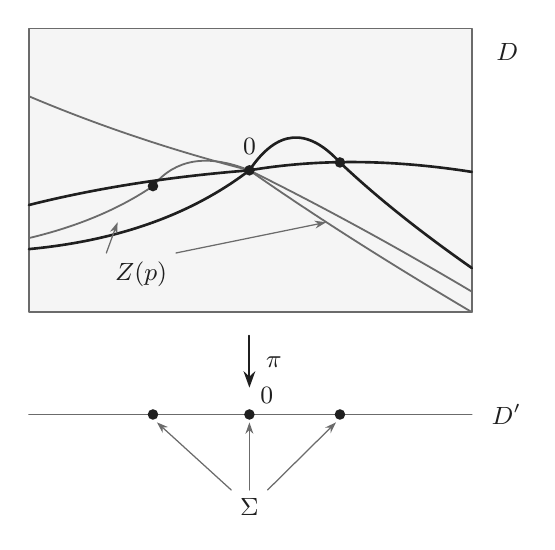
\begin{tikzpicture}[field/diagram, x=0.025cm, y=0.020cm]
    \fill[FieldPaper] (10,120) rectangle (235,300);
    \draw[field/secondary] (10,120) rectangle (235,300);
    \node[right] at (243,285) {$D$};
    \draw[field/secondary]
        (10,257) .. controls (45.33,238.33) and (82.67,222.67) .. (122,210)
        .. controls (154,182) and (191.67,152) .. (235,120);
    \draw[field/curve]
        (10,160) .. controls (55.33,165.33) and (92.67,182) .. (122,210)
        .. controls (136,236) and (151.33,237.67) .. (168,215)
        .. controls (186,193.67) and (208.33,171.33) .. (235,148);
    \draw[field/secondary]
        (10,167) .. controls (34.67,174.33) and (55.67,185.33) .. (73,200)
        .. controls (84.33,217.33) and (100.67,220.67) .. (122,210)
        .. controls (158.67,187.33) and (196.33,161.67) .. (235,133);
    \draw[field/curve]
        (10,188) .. controls (44,198.67) and (81.33,206) .. (122,210)
        .. controls (156.67,217.33) and (194.33,217) .. (235,209);
    \foreach \x/\y in {73/200,122/210,168/215} {
        \node[field/point] at (\x,\y) {};
    }
    \node[above, inner sep=4pt] at (122,211) {$0$};
    \node (Z) at (67,144) {$Z(p)$};
    \draw[field/leader] (Z.north west) -- (55,177);
    \draw[field/leader] (Z.north east) -- (161,177);
    \draw[field/map] (122,105) -- (122,72)
        node[midway, right, inner sep=5pt] {$\pi$};
    \draw[field/secondary] (10,55) -- (235,55)
        node[right, xshift=4pt] {$D'$};
    \foreach \x in {73,122,168} {
        \node[field/point] at (\x,55) {};
    }
    \node[above right, inner sep=3pt] at (122,55) {$0$};
    \node (Sigma) at (122,-4) {$\Sigma$};
    \draw[field/leader] (Sigma.north west) -- (75,50);
    \draw[field/leader] (Sigma.north) -- (122,50);
    \draw[field/leader] (Sigma.north east) -- (166,50);
\end{tikzpicture}

        \FieldCaption{I}{6}{}
    \end{minipage}
\end{center}
At each point $z'_0\in D'\setminus\Sigma$, $p(z'_0,z_n)$ has precisely $p$ distinct roots. Denote these roots by $\lambda_1(z'_0),\ldots,\lambda_p(z'_0)$. Since $\delta(z'_0)\ne0$, $\frac{\partial p}{\partial z_n}(z'_0,\lambda_j(z'_0))\ne0$, $1\leq j\leq n$, and we may apply the implicit function theorem to deduce that the roots $\lambda_j$ depend analytically on $z'$, $z'\notin\Sigma$ (see Remark 4, \hyperref[sec:2:1]{\S1 of Chapter 2}). It follows that $Z(p)\setminus\pi^{-1}(\Sigma)$ is a (complex) submanifold of $D$ of complex codimension 1 (see Chapter~\ref{ch:4} for terminology). Moreover, $\pi$ clearly restricts to a $p$-fold covering map of $Z(p)\setminus\pi^{-1}(\Sigma)$ over $D'\setminus\Sigma$. The zero set $Z(p)$ may have ``singularities'' (points where $Z(p)$ fails to be a submanifold of $D$) at points lying over $\Sigma$.
\paragraph*{Examples.}
\begin{enumerate}
\item Let $f(z,w)=z^2-w^3$. Then $f_0$ is prime and is a Weierstrass polynomial in $z$. The discriminant locus of $f$ is the origin of $\mathbb C$ (the $w$-axis). The reader may verify that at the origin of $\mathbb C^2$ it is not possible to find a submanifold chart (analytic or $C^\infty$) for $Z(f)$. However, $Z(f)$ is a topological manifold as the map $t\mapsto(t^3,t^2)$ defines a homeomorphism of $\mathbb C$ onto $Z(f)$.
\item Let $f(u,v,w)=u^{2p}-vw$, for some positive integer $p$. Then $f_0$ is prime and is a Weierstrass polynomial in $u$. The discriminant locus
% Original book page 118
of $f$ is the origin of the $(v,w)$-plane. We claim that $Z(f)$ is not a topological manifold. If it were, it would have to be modelled on $\mathbb C^2$ since $Z(f)\setminus\{0\}$ is of complex dimension 2. Moreover, since $\mathbb C^2\setminus\{0\}$ is simply connected, it would be possible to find simply connected neighbourhoods of $0$ in $Z(f)\setminus\{0\}$. But the map $\phi:\mathbb C^2\setminus\{0\}\to Z(f)\setminus\{0\}$ defined by $\phi(t,s)=(ts,t^p,s^p)$ is a $p$-fold covering map. Hence there is no neighbourhood of zero in $Z(f)\setminus\{0\}$ which is simply connected and so $Z(f)$ cannot be a topological manifold.
\end{enumerate}
We shall now make a more general study of the local structure of analytic sets. Our approach is close to that given in Gunning and Rossi \cite{bib:I:gunning-r-c-and-rossi-h:1}. We start by defining the germ at a point of a subset of $\mathbb C^n$. Suppose $X,Y$ are subsets of $\mathbb C^n$. We say that $X$ and $Y$ are equivalent at $a\in\mathbb C^n$ if there exists $U\in\mathcal U_a$ such that $X\cap U=Y\cap U$. This relation is certainly an equivalence relation on subsets of $\mathbb C^n$. We denote the equivalence class of a subset $X$ by $X_a$ and refer to $X_a$ as the \emph{germ} of $X$ at $a$.

If $\alpha$ and $\beta$ are germs of sets at $a$, we define
\[\alpha\cup\beta=(X\cup Y)_a;\quad\alpha\cap\beta=(X\cap Y)_a;\quad\alpha-\beta=(X\setminus Y)_a,\]
where $X$ and $Y$ are representatives for $\alpha$ and $\beta$ respectively. Just as for germs of functions, it is easy to verify that the finite union, intersection and difference of germs of sets are well defined. As an exercise, the reader may show that arbitrary unions or intersections of germs of sets need not be well defined.

We write $\alpha\subset\beta$, if there exist representatives $X$ and $Y$ of $\alpha$ and $\beta$ respectively such that $X\subset Y$.

Suppose $f_a\in\mathcal O_a^p$. Choose a representative $f=(f_1,\ldots,f_p)$ for $f_a$. We let $Z(f_a)$ denote the germ of $Z(f)$ at $a$. That is, $Z(f_a)=f^{-1}(0)_a$. $Z(f_a)$ clearly depends only on $f_a$ and not on the choice of representative function for $f_a$. We let $\mathcal A_a$ denote the set of all germs\IndexMark{idx-268}{germ@Germ!set@set} at $a$ of analytic sets. Thus $X_a\in\mathcal A_a$ if and only if there exists $f_a\in\mathcal O_a^p$ such that $X_a=Z(f_a)$.
% Original book page 119
\FieldHeading{Lemma}{3.5.1}{}\FieldTarget{lemma:3.5.1}{3.5.1} Suppose $f=(f_1,\ldots,f_p)$ is a representative function for $f_a\in\mathcal O_a^p$. Then
\begin{align*}
Z(f_a)&=\bigcap_{i=1}^p Z(f_i)_a\\
&=\bigcap_{i=1}^p Z(f_{i,a}).
\end{align*}
(Here $f_{i,a}$ denotes the germ of $f_i$ at $a$).
\begin{proof}Trivial.\end{proof}
\paragraph*{Notation.} If $f=(f_1,\ldots,f_p)\in A(U)^p$, we shall adopt the conventions that $Z(f_1,\ldots,f_p)=Z(f)$ and $Z(f_{1,a},\ldots,f_{p,a})=Z(f_1,\ldots,f_p)_a=Z(f)_a$.
\FieldHeading{Proposition}{3.5.2}{}\FieldTarget{proposition:3.5.2}{3.5.2} Let $X_a,Y_a\in\mathcal A_a$. Then $X_a\cup Y_a$, $X_a\cap Y_a\in\mathcal A_a$.
\begin{proof}
We may suppose that $X_a=Z(f_1,\ldots,f_p)$, $Y_a=Z(g_1,\ldots,g_q)$ for suitable $f_i,g_j\in\mathcal O_a$. Clearly
\begin{align*}
X_a\cup Y_a&=Z(f_ig_j:1\leq i\leq p,\ 1\leq j\leq q),\\
X_a\cap Y_a&=Z(f_1,\ldots,f_p,g_1,\ldots,g_q).
\end{align*}
\end{proof}
\FieldHeading{Definition}{3.5.3}{}\FieldTarget{definition:3.5.3}{3.5.3} Suppose $X_a\in\mathcal A_a$. We say $f_a\in\mathcal O_a$ \emph{vanishes on $X_a$} if for some representatives $X$ of $X_a$ and $f$ of $f_a$ we have $f|X\equiv0$. We write $f_a=0$ on $X_a$.
\FieldHeading{Definition}{3.5.4}{}\FieldTarget{definition:3.5.4}{3.5.4} Let $X_a\in\mathcal A_a$. We define
\[I(X_a)=\{f_a\in\mathcal O_a:f_a=0\text{ on }X_a\}.\]
\FieldHeading{Proposition}{3.5.5}{}\FieldTarget{proposition:3.5.5}{3.5.5} Let $X_a\in\mathcal A_a$. Then $I(X_a)$ is an ideal of $\mathcal O_a$.
\begin{proof}Trivial.\end{proof}
\paragraph*{Notation.} We write $I\lhd\mathcal O_a$ to signify that $I$ is an ideal of $\mathcal O_a$.
% Original book page 120
\paragraph*{Example.} Let $X$ be an analytic subset of the domain $\Omega$ in $\mathbb C^n$. For each $a\in\Omega$, we set $I_a(X)=I(X_a)$. Then $I_a(X)\lhd\mathcal O_a$ for every $a\in\Omega$. If $a\notin X$, $I_a(X)=\mathcal O_a$.

Before stating the next proposition recall that if $R$ is a commutative ring and $I\lhd R$, then the \emph{radical}\IndexMark{idx-498}{radical of ideal@Radical (of ideal)} of $I$, $\operatorname{Rad}(I)$, is defined by
\[\operatorname{Rad}(I)=\{r\in R:\text{For some positive integer }p,\ r^p\in I\}.\]
\FieldHeading{Proposition}{3.5.6}{}\FieldTarget{proposition:3.5.6}{3.5.6} For every germ $X_a\in\mathcal A_a$
\[I(X_a)=\operatorname{Rad}(I(X_a)).\]
\begin{proof}If $f_a^p$ vanishes on $X_a$ then certainly $f_a$ vanishes on $X_a$.\end{proof}
\FieldHeading{Proposition}{3.5.7}{}\FieldTarget{proposition:3.5.7}{3.5.7} Let $I$ be an ideal in $\mathcal O_a$ and let $\{a_1,\ldots,a_p\}$ be a finite set of generators for $I$. Then
\begin{enumerate}
\item If $f\in I$, $f$ vanishes on $Z(a_1,\ldots,a_p)$.
\item $Z(a_1,\ldots,a_p)$ depends only on $I$ and not on the particular choice of generators for $I$.
\end{enumerate}
\begin{proof}
Let $f\in I$. Then $f=\sum_{j=1}^p f_ja_j$, $f_j\in\mathcal O_a$, $1\leq j\leq p$. Hence $f\in Z(a_1,\ldots,a_p)$, proving 1. Statement 2 follows straightforwardly from 1.
\end{proof}
\FieldHeading{Definition}{3.5.8}{}\FieldTarget{definition:3.5.8}{3.5.8} Suppose $I\lhd\mathcal O_a$. We define
\[Z(I)=Z(a_1,\ldots,a_p),\]
where $\{a_1,\ldots,a_p\}$ is any finite set of generators for $I$.

It follows from Propositions~\ref{proposition:3.5.6} and \ref{proposition:3.5.7} that we have a correspondence between radical ideals in $\mathcal O_a$ and germs of analytic sets. In the next theorem we list further properties of this correspondence.
% Original book page 121
\FieldHeading{Theorem}{3.5.9}{}\FieldTarget{theorem:3.5.9}{3.5.9}
\begin{enumerate}
\item[1.] If $X_a,Y_a\in\mathcal A_a$ and $X_a\subset Y_a$ then $I(X_a)\supset I(Y_a)$.
\item[$1'$.] If $I,J\lhd\mathcal O_a$ and $I\subset J$ then $Z(I)\supset Z(J)$.
\item[2.] If $X_a,Y_a\in\mathcal A_a$ and $X_a\ne Y_a$ then $I(X_a)\ne I(Y_a)$.
\item[3.] If $X_a\in\mathcal A_a$, $I(X_a)=\operatorname{Rad}(I(X_a))$.
\item[$3'$.] If $I\lhd\mathcal O_a$, $Z(I)=Z(\operatorname{Rad}(I))$.
\item[4.] If $X_a\in\mathcal A_a$, then $Z(I(X_a))=X_a$.
\item[$4'$.] If $I\lhd\mathcal O_a$, $I(Z(I))\supseteq\operatorname{Rad}(I)$.
\end{enumerate}
\begin{proof}
We shall prove statements 2, 4 and $4'$. Statement 3 is Proposition~\ref{proposition:3.5.6}. We leave the remaining cases as exercises for the reader (the full proof may be found in Gunning and Rossi \cite{bib:I:gunning-r-c-and-rossi-h:1}).

Proof of 2. For some $U\in\mathcal U_a$ and $f_j\in A(U)$, $1\leq j\leq p+q$, we may write $X=Z(f_1,\ldots,f_p)$, $Y=Z(f_{p+1},\ldots,f_{p+q})$, where $X,Y$ are representatives for $X_a,Y_a$ respectively. Since $X_a\ne Y_a$, we may find $z_W\in((X\setminus Y)\cup(Y\setminus X))\cap W$ for every $W\in\mathcal U_a$. Hence there exists $j(W)\in\{1,\ldots,p+q\}$ such that $f_{j(W)}(z_W)\ne0$. This is true for all sufficiently small neighbourhoods $W$ of $a$ and so there must exist a $j_0$ such that $f_{j_0}$ does not vanish identically on $((X\setminus Y)\cup(Y\setminus X))\cap W$ for any $W\in\mathcal U_a$. If $1\leq j_0\leq p$, this implies $f_{j_0}\ne0$ on $Y_a$ and if $p+1\leq j_0\leq p+q$, $f_{j_0}\ne0$ on $X_a$. Hence $I(X_a)\ne I(Y_a)$.

Proof of 4. If $f_a\in I(X_a)$ then certainly $f_a=0$ on $X_a$ and so $Z(I(X_a))\supseteq Z_a$. On the other hand we may write $X_a=Z(f_1,\ldots,f_k)$ for some $f_j\in\mathcal O_a$. Since $f_j=0$ on $X_a$, $f_j\in I(X_a)$ and so $Z(f_j)\supseteq Z(I(X_a))$. This holds for all $j$ and so $X_a=Z(f_1,\ldots,f_k)\supseteq Z(I(X_a))$.

Proof of $4'$. Obviously, $I(Z(I))\supseteq I$ for any $I\lhd\mathcal O_a$. By $3'$, $Z(I)=Z(\operatorname{Rad}(I))$ and so $I(Z(I))=I(Z(\operatorname{Rad}(I)))\supseteq\operatorname{Rad}(I)$.
\end{proof}
\paragraph*{Remark.} A consequence of Theorem~\ref{theorem:3.5.9} is that the map $X_a\to I(X_a)$ is injective into the set of radical ideals in $\mathcal O_a$ with left inverse defined by mapping $I$ to $Z(I)$, for radical $I\lhd\mathcal O_a$. To show that this map is onto we need to know that $I(Z(I))=I$ for all radical ideals $I$ of $\mathcal O_a$ and not just that $I(Z(I))\supseteq I$ (condition $4'$). In fact we do have equality and this fundamental result is the \emph{Nullstellensatz}\IndexMark{idx-412}{nullstellensatz@Nullstellensatz}
% Original book page 122
for germs of analytic sets. The proof of the Nullstellensatz lies much deeper than the other results of this section and may be found in Gunning and Rossi \cite{bib:I:gunning-r-c-and-rossi-h:1}, Gunning \cite{bib:I:gunning-r-c:1}, Herv\'e \cite{bib:I:herve-m:1} or R. Narasimhan \cite{bib:I:narasimhan-r:3}. We shall prove a special case, the Nullstellensatz for principal ideals, later in this section and this will suffice for our intended applications.
\FieldHeading{Definition}{3.5.10}{}\FieldTarget{definition:3.5.10}{3.5.10} We say that a germ $X_a\in\mathcal A_a$ is \emph{irreducible}\IndexMark{idx-340}{irreducible@Irreducible!germ@germ} if whenever $X_a=Y_a\cup Z_a$, $Y_a,Z_a\in\mathcal A_a$, we have either $X_a=Y_a$ or $X_a=Z_a$.
\FieldHeading{Theorem}{3.5.11}{}\FieldTarget{theorem:3.5.11}{3.5.11} A germ $X_a$ is irreducible if and only if $I(X_a)$ is prime.
\begin{proof}
Suppose $I(X_a)$ is not prime. Then there exist $f,g\in\mathcal O_a$ such that $fg\in I(X_a)$ but neither $f$ nor $g$ lie in $I(X_a)$. Now $X_a=X_a\cap Z(fg)=X_a\cap(Z(f)\cup Z(g))=(X_a\cap Z(f))\cup(X_a\cap Z(g))$. Since $f,g\notin I(X_a)$, $X_a\cap Z(f)$ and $X_a\cap Z(g)$ are strictly contained in $X_a$ and so $X_a$ is not irreducible. Conversely, suppose that $X_a$ is not irreducible. Then $X_a=Y_a\cup Z_a$, where $Y_a$ and $Z_a$ are strictly contained in $X_a$. By 2 of Theorem~\ref{theorem:3.5.9}, $I(Y_a),I(Z_a)\ne I(X_a)$ and so, by 1 of Theorem~\ref{theorem:3.5.9}, $I(Y_a),I(Z_a)$ strictly contain $I(X_a)$. Pick $f\in I(Y_a)\setminus I(X_a)$, $g\in I(Z_a)\setminus I(X_a)$. Since $fg\in I(Y_a)\cap I(Z_a)=I(X_a)$, we see that $I(X_a)$ is not prime.
\end{proof}
\FieldHeading{Theorem}{3.5.12}{}\FieldTarget{theorem:3.5.12}{3.5.12} Let $X_a\in\mathcal A_a$. We may decompose $X_a$ into a finite union $X_a^1\cup\cdots\cup X_a^k$ of irreducible germs satisfying
\begin{enumerate}
\item $X_a^j\not\subset\bigcup_{i\ne j}X_a^i$ for $j=1,\ldots,k$.
\item The $X_a^i$ are uniquely determined (up to order) by $X_a$.
\end{enumerate}
\begin{proof}
Set $I=I(X_a)$. It follows from the theory of Noetherian rings that we may write $I=\bigcap_{j=1}^s I_j$, where the $I_j$ are primary ideals (that is, $\operatorname{rad}(I_j)$ is prime). See, for example, Van der Waerden \cite{bib:I:waerden-b-l-van-der:2} or Zariski and Samuel \cite{bib:I:zariski-o-and-samuel-p:1}. Set $P_j=\operatorname{Rad}(I_j)$. By 4 of Theorem~\ref{theorem:3.5.9}, $X_a=Z(I)=\bigcup_{j=1}^s Z(P_j)$. We may throw away any germs $Z(P_j)$ which are contained in the union of the remaining germs to obtain the required decomposition of $X_a$ as a union of irreducible germs. Suppose that
% Original book page 123
$X_a=X_a^1\cup\cdots\cup X_a^k=Y_a^1\cup\cdots\cup Y_a^p$ are two decompositions of $X_a$ as unions of irreducible germs which satisfy condition 1 of the theorem. For $j\in\{1,\ldots,k\}$, $X_a^j=\bigcup_{i=1}^p(Y_a^i\cap X_a^j)$ and since $X_a^j$ is irreducible, we must have $X_a^j=Y_a^{\tau(j)}\cap X_a^j$ for some $\tau(j)\in\{1,\ldots,p\}$. Hence $X_a^j\subset Y_a^{\tau(j)}$, $1\leq j\leq k$. Similarly, $Y_a^i\subset X_a^{\rho(i)}$ for some $\rho(i)\in\{1,\ldots,k\}$, $1\leq i\leq p$. It follows that for all $i,j$ we have
\[X_a^j\subset Y_a^{\tau(j)}\subset X_a^{\rho\tau(j)}\quad\text{and}\quad Y_a^i\subset X_a^{\rho(i)}\subset Y_a^{\tau\rho(i)}.\]
Since the decompositions satisfy condition 1, $\rho\tau$ and $\tau\rho$ are the identity maps. Therefore $k=p$ and $X_a^j=Y_a^{\tau(j)}$, $1\leq j\leq k$.
\end{proof}
We conclude this section by proving three results about germs of analytic sets whose ideals are principal.
\FieldHeading{Theorem}{3.5.13}{ (Nullstellensatz for principal prime ideals).}\FieldTarget{theorem:3.5.13}{3.5.13} Let $f_a\in\mathcal O_a$ be irreducible. Then $I(Z(f_a))=(f_a)$.
\begin{proof}
From $4'$ of Theorem~\ref{theorem:3.5.9} we already know that $I(Z(f_a))\supset(f_a)$. If $g_a\notin(f_a)$, then $(f_a,g_a)=1$ since $f_a$ is irreducible. Let $f$ and $g$ be representatives for $f_a$ and $g_a$ respectively. By Lemma~\ref{lemma:3.4.3}, we may find $z$ arbitrarily close to $a$ such that $f(z)=0$ and $g(z)\ne0$. Hence $g_a\notin I(Z(f_a))$. Therefore $I(Z(f_a))\subset(f_a)$.
\end{proof}
\FieldHeading{Corollary}{3.5.14}{ (Nullstellensatz for principal ideals).}\IndexMark{idx-413}{nullstellensatz@Nullstellensatz!for principal ideals@for principal ideals}\FieldTarget{corollary:3.5.14}{3.5.14} Let $f_a\in\mathcal O_a$. Then $I(Z(f_a))=\operatorname{Rad}((f_a))$.
\begin{proof}
Write $f_a=p_1^{r_1}\cdots p_s^{r_s}$, where the $p_j\in\mathcal O_a$ are irreducible and distinct. We certainly have $Z(f_a)=\bigcup_{i=1}^s Z(p_i)$ and so, by Theorem~\ref{theorem:3.5.13}, $I(Z(f_a))=\bigcap_{i=1}^s(p_i)=\operatorname{Rad}(f_a)$.
\end{proof}
\FieldHeading{Corollary}{3.5.15}{}\FieldTarget{corollary:3.5.15}{3.5.15} Let $p_s^{r_1}\cdots p_s^{r_s}$ be the prime factorization of $f_a\in\mathcal O_a$. Then $Z(f_a)=\bigcup_{i=1}^s Z(p_i)$ is the unique decomposition of $Z(f_a)$ into irreducible germs given by Theorem~\ref{theorem:3.5.12}.
\begin{proof}
All we need to check is that for every $i$, $Z(p_i)\not\subset\bigcup_{j\ne i}Z(p_j)$. By the Nullstellensatz for principal prime ideals, this condition is
% Original book page 124
equivalent to $(p_i)\not\supset(p_1\cdots p_{i-1}p_{i+1}\cdots p_s)$. This is certainly true since $p_i$ is not divisible by $p_j$, $i\ne j$.
\end{proof}
\FieldHeading{Theorem}{3.5.16}{}\FieldTarget{theorem:3.5.16}{3.5.16} Let $U$ be a domain in $\mathbb C^n$ and suppose that $f\in A(U)$ is not identically zero. Set $X=f^{-1}(0)$. Given $x\in X$, suppose that $p_x$ is a generator of the principal ideal $I_x(X)$. Then we can choose a representative $p$ for $p_x$, defined on some neighbourhood $V$ of $x$ in $U$, such that $I_y(X)=(p_y)$ for all $y\in V$.
\begin{proof}
It is clearly sufficient to prove the result for the special case when $p_x$ is irreducible. Changing coordinates and multiplying by a unit we may assume that $x=0$ and that we may find a polydisc neighbourhood $D'$ of $0$ in $\mathbb C^{n-1}$ and $s>0$ such that if $D=\{z\in\mathbb C^n:z'\in D',\ |z_n|<s\}$, then $p_0$ is the germ of a Weierstrass polynomial $p$ on $D$:
\[p(z',z_n)=z_n^p+\sum_{j=0}^{p-1}a_j(z')z_n^j.\]
Assuming that $D\subset U$, we have $p^{-1}(0)=X\cap D$. The discriminant locus $\Sigma$ of $p$ is a proper analytic subset of $D$ and so, in particular, $D'\setminus\Sigma$ is an open dense subset of $D'$. If $y=(y',y_n)\in p^{-1}(0)$ and $y'\notin\Sigma$, then $\partial p/\partial z_n(y',y_n)\ne0$. Consequently $p_y$ is irreducible (See Exercise 2, \hyperref[sec:3:3]{\S3}). On the other hand suppose that $y=(y',y_n)\in p^{-1}(0)$ and $y'\in\Sigma$. Let $\phi_y$ be a generator of $I_y(X)$. Then for some positive integer $k$ and unit $u_y\in\mathcal O_y$, $p_y=u_y\phi_y^k$. This equation holds on a neighbourhood of $y$ in $D$ and so holds for points $z=(z',z_n)\in p^{-1}(0)$ with $z'\notin\Sigma$. Consequently, $k=1$. Our arguments prove that $I_y(X)=(p_y)$ for all $y\in D$.
\end{proof}
\paragraph*{Remark.} Theorem~\ref{theorem:3.5.16} is a special case of the fundamental coherence theorem of H. Cartan which asserts that if $g_x^1,\ldots,g_x^k$ generate $I_x(X)$ then $g_y^1,\ldots,g_y^k$ generate $I_y(X)$ for $y$ in some neighbourhood of $x$. Here $X$ is an arbitrary analytic subset. The proof of this result is considerably harder than the special case given above and the reader may find proofs in H. Cartan \cite{bib:I:cartan-h:2}, Gunning and Rossi \cite{bib:I:gunning-r-c-and-rossi-h:1}, R. Narasimhan \cite{bib:I:narasimhan-r:3} and Whitney \cite{bib:I:whitney-h:1}.
% Original book page 125
\subsection*{Exercises}
\begin{enumerate}
\item Suppose $p(z',z_n)$ is an irreducible Weierstrass polynomial of degree $p$ defined on the polydisc $D=D'\times D_s(0)$, with discriminant $\delta\in A(D')$ and discriminant locus $\Sigma$. Let $\pi:D\to D'$ denote the projection on $D'$ and set $X=p^{-1}(0)$.
\begin{enumerate}
\item[i)] Suppose $Y$ is a connected component of $X\setminus\pi^{-1}(\Sigma)$. Show that $\pi|Y$ is an $s$-fold cover of $D'\setminus\Sigma$ for some $s$, $1\leq s\leq p$. (Hint: Fix $z'_0\in D'\setminus\Sigma$ and a root $\lambda_j(z'_0)\in Y$. Consider the unique lifts through $\lambda_j(z'_0)$ of all closed paths in $D'\setminus\Sigma$ starting at $z'_0$. Note that $D'\setminus\Sigma$ is connected (Corollary~\ref{corollary:2.2.3})).
\item[ii)] Using the analyticity of the roots of $p(z',z_n)$ together with the Riemann removable singularities theorem, prove that $\overline Y$ is the zero locus of a polynomial in $z_n$ with coefficients analytic in $z'\in D'$.
\item[iii)] Deduce from ii) that $\overline Y=X$ and that $X\setminus\pi^{-1}(\Sigma)$ is connected.
\end{enumerate}
\item Suppose that $f(y,z)$ is a Weierstrass polynomial in $z$ of degree $p$ defined on an open polydisc $D_a(0)\times D_b(0)\subset\mathbb C^2$ and that the discriminant locus is equal to $\{0\}\subset D_a(0)$. Set $c=a^{1/p}$. Show that
\begin{enumerate}
\item[i)] There exists an analytic function $\phi:D_c(0)\to\mathbb C$ such that $f(t^p,\phi(t))=0$, $t\in D_c(0)$.
\item[ii)] If $\omega=\exp(2\pi i/p)$, then given $y=t^p\in D_a(0)$, $f(y,z)=0$ if and only if $z=\phi(\omega^jt)$ for some integer $j$, $a\leq j\leq p-1$. (Hint for i): Define $\gamma:D_c(0)\to D_a(0)$ by $\gamma(t)=t^p$. Now show using Q1 and the Riemann removable singularities theorem that lifts to an analytic map $\widetilde\gamma:D_c(0)\to D_a(0)\times D_b(0)$ with image $X$). (Observe that if $y=t^p$ and we define $y^{r/p}=t^r$ then we obtain the \emph{fractional power series}\IndexMark{idx-258}{fractional power series@Fractional power series}\IndexMark{idx-484}{puiseux series@Puiseux series} or \emph{Puiseaux series} solution $z=\phi(y^{1/p})$ to $f(y,z)=0$. Further details may be found in Walker \cite{bib:I:walker-r:1}).
\end{enumerate}
\item Let $f=(f_1,\ldots,f_p)\in\mathcal O_0^p$. Show that if $Df(0)$ is of maximal rank then $Z(f)$ is irreducible.
\end{enumerate}
% Original book page 126
\section{\texorpdfstring{Modules over $\mathcal O_0$}{Modules over O0}}\label{sec:3:6}
Suppose that $M$ is a finitely generated $\mathcal O_0$-module. Let $U_1^0,\ldots,U_{p(0)}^0$ be a set of generators for $M$ and define $U^0:\mathcal O_0^{p(0)}\to M$ by $U^0(f_1,\ldots,f_{p(0)})=\sum_{j=1}^{p(0)}f_jU_j^0$. The sequence $\mathcal O_0^{p(0)}\xrightarrow{U^0}M\to0$ is exact. The kernel of $U^0$, $\operatorname{Ker}(U^0)$, is a submodule of $\mathcal O_0^{p(0)}$ and so, by Lemma~\ref{lemma:3.3.5}, is finitely generated. If $U_1^1,\ldots,U_{p(1)}^1$ is a set of generators for $\operatorname{Ker}(U^0)$ we may repeat the above construction to obtain an exact sequence $\mathcal O_0^{p(1)}\xrightarrow{U^1}\mathcal O_0^{p(0)}\xrightarrow{U^0}M\to0$. Iterating this construction we obtain a long exact sequence
\[\cdots\xrightarrow{U^{n+1}}\mathcal O_0^{p(n)}\xrightarrow{U^n}\cdots\xrightarrow{U^1}\mathcal O_0^{p(0)}\xrightarrow{U^0}M\to0.\]
Such a sequence is called a \emph{free resolution}\IndexMark{idx-261}{free resolution@Free resolution} of $M$ (it is also referred to as a \emph{chain of syzygies} for $M$---see Gunning and Rossi \cite{bib:I:gunning-r-c-and-rossi-h:1} or Nagata \cite{bib:I:nagata-m:1}). Suppose that for some $s$, $\operatorname{Ker}(U^{s-1})$ is a \emph{free} $\mathcal O_0$-module. That is, $\operatorname{Ker}(U^{s-1})\cong\mathcal O_0^q$ for some integer $q$. Then we may replace the original free resolution by the finite free resolution
\[0\to\mathcal O_0^q\xrightarrow{\mu}\mathcal O_0^{p(s-1)}\longrightarrow\cdots\to\mathcal O_0^{p(0)}\to M\to0,\]
where $\mu$ denotes an isomorphism of $\mathcal O_0^q$ onto $\operatorname{Ker}(U^{s-1})$. Such a finite free resolution of $M$ is said to have \emph{length}\IndexMark{idx-356}{length of resolution@Length (of resolution)} $s$.
\FieldHeading{Theorem}{3.6.1}{ (Hilbert Syzygy theorem).}\IndexMark{idx-290}{hilbert syzygy theorem@Hilbert Syzygy theorem}\IndexMark{idx-597}{syzygy theorem@Syzygy theorem}\FieldTarget{theorem:3.6.1}{3.6.1} Every $\mathcal O_0$-module has a free resolution of\IndexMark{idx-508}{resolution of module@Resolution of module} length $n$.
\begin{proof}
It is sufficient to show that for any free resolution of $M$,
\[\xrightarrow{U^s}\mathcal O_0^{p(s-1)}\xrightarrow{U^{s-1}}\cdots\xrightarrow{U^1}\mathcal O_0^{p(0)}\xrightarrow{U^0}M\to0,\]
$\operatorname{Ker}(U^{n-1})$ is free.

To simplify notation, we set $K_s=\operatorname{Ker}(U^s)$ and let $M_s$ denote the ideal of $\mathcal O_0$ generated by $z_1,\ldots,z_s$. In particular, $M_n=\mathfrak m_0$, the maximal ideal of $\mathcal O_0$.
% Original book page 127
\paragraph*{Step 1.} For $s\geq j$, we have $K_s\cap M_j\mathcal O_0^{p(s)}=M_jK_s$. Obviously, we have $K_s\cap M_j\mathcal O_0^{p(s)}\supset M_jK_s$ and so it remains to verify the reverse inclusion. Our proof goes by induction on $j$. Suppose $j=1$, and that $f\in K_s\cap M_1\mathcal O_0^{p(s)}$. Then $f=z_1g$, $g\in\mathcal O_0^{p(s)}$. Since $U^s(f)=0$, $z_1U^s(g)=0$ and so $U^s(g)=0$. Therefore $g\in K_s$ and $f\in M_1K_s$. Now suppose that we have proved the result for $j-1$ and all $s\geq j-1$. Let $f\in K_s\cap M_j\mathcal O_0^{p(s)}$. Then $f=z_1g_1+\cdots+z_jg_j$, $g_1,\ldots,g_j\in\mathcal O_0^{p(s)}$. Since $f\in K_s$, $U^s(f)=z_1U^s(g_1)+\cdots+z_jU^s(g_j)=0$. Therefore, $z_jU^s(g_j)=-(z_1U^s(g_1)+\cdots+z_{j-1}U^s(g_{j-1}))$ and so, dividing through by $z_j$ we see that $U^s(g_j)\in M_{j-1}\mathcal O_0^{p(s-1)}$. Now $U^{s-1}U^s=0$ and so $U^s(g_j)\in K_{s-1}\cap M_{j-1}\mathcal O_0^{p(s-1)}$. By the inductive hypothesis, $U^s(g_j)\in M_{j-1}K_{s-1}$. Since $K_{s-1}=\operatorname{Image}(U^s)$, there exist $h_1,\ldots,h_{j-1}\in\mathcal O_0^{p(s)}$ such that
\[U^s(g_j)=z_1U^s(h_1)+\cdots+z_{j-1}U^s(h_{j-1}).\]
Now set $h_j=g_j-z_1h_1-\cdots-z_{j-1}h_{j-1}$. Certainly $h_j\in K_s$. We claim that $f-z_jh_j\in M_{j-1}K_s$. This follows from the inductive hypothesis since $f-z_jh_j=\sum_{i=1}^{j-1}z_i(g_i+z_jh_i)$ and so $f-z_jh_j\in K_s\cap M_{j-1}\mathcal O_0^{p(s)}=K_sM_{j-1}$. Since $h_j\in K_s$, $f\in M_jK_s$.
\paragraph*{Step 2.} Choose a set of generators $U_1,\ldots,U_q$ for $K_{n-1}$ which is minimal---that is, no proper subset of $U_1,\ldots,U_q$ generates $K_{n-1}$. Define $U:\mathcal O_0^q\to\mathcal O_0^{p(n-1)}$ by $U(f_1,\ldots,f_q)=\sum_{j=1}^q f_jU_j$. We claim that $U$ is an isomorphism onto $K_{n-1}$. For this it is sufficient to verify that $\operatorname{Ker}(U)$ is zero.

Modify the original free resolution of $M$ at the $n$th step to obtain the new free resolution
\[\mathcal O_0^q\xrightarrow{U}\mathcal O_0^{p(n-1)}\xrightarrow{U^{n-1}}\cdots\xrightarrow{U^0}M\to0.\]
Applying Step 1 to this resolution with $j=n$ we see that
\[\operatorname{Ker}(U)\cap\mathfrak m_0\mathcal O_0^q=\mathfrak m_0\operatorname{Ker}(u).\]
In fact, $\operatorname{Ker}(U)\subset\mathfrak m_0\mathcal O_0^q$. To see this, suppose $(f_1,\ldots,f_q)\in\operatorname{Ker}(U)\subset\mathcal O_0^q$. Then
% Original book page 128
\[0=U(f_1,\ldots,f_q)=\sum_{j=1}^q f_jU_j.\]
Since $U_1,\ldots,U_q$ is a minimal set of generators, no $f_j$ can be a unit. That is, $f_j\in\mathfrak m_0$, $1\leq j\leq q$.

We have now shown that $\operatorname{Ker}(U)=\mathfrak m_0\operatorname{Ker}(U)$. This implies that $\operatorname{Ker}(U)=0$, for otherwise we may find $a_{ij}\in\mathfrak m_0$ such that
\[U_i=\sum_{i=1}^q a_{ij}U_j.\]
Therefore $\det[\delta_{ij}-a_{ij}]=0$ and so, expanding the determinant, we see that $1\in\mathfrak m_0$ which is a contradiction.
\end{proof}
\paragraph*{Remark.} The last paragraph of the proof of Theorem~\ref{theorem:3.6.1} is a special case of
\paragraph*{Nakayama's Lemma:}\IndexMark{idx-406}{nakayama s lemma@Nakayama's Lemma} Let $R$ be a local ring with maximal ideal $\mathfrak m$ and $M$ be a finite $R$-module. Then
\begin{enumerate}
\item[a)] If $M=\mathfrak mM$, $M=0$.
\item[b)] If $N$ is a submodule of $M$ such that $M=N+\mathfrak mM$, $N=M$.
\end{enumerate}
The proof of a) is the same as that used in the last paragraph of the proof of Theorem~\ref{theorem:3.6.1}. Statement b) follows by applying a) to $M/N$.

Suppose that $M$ is a submodule of $\mathcal O_0^p$. Since $\mathcal O_0$ is Noetherian, $M$ has a finite set of generators $U_1,\ldots,U_q$ and so we have an exact sequence $\mathcal O_0^q\xrightarrow{U}M\to0$ where $U$ is defined by mapping $(f_1,\ldots,f_q)$ to $\sum_{j=1}^q f_jU_j$. The question naturally arises as to whether this sequence is \emph{split} exact. Certainly it is not generally split exact as a sequence of $\mathcal O_0$-modules! However, it makes sense to ask whether it splits as a sequence of vector spaces. That is, can we find a $\mathbb C$-linear map $\xi:M\to\mathcal O_0^q$ such that $U\xi$ is the identity map of $M$? Equivalently, can we write every $m\in M$ in the form $\sum\xi_i(m)U_i$, where $\xi_i$ is linear, $1\leq i\leq q$? In view of the continuity conditions in the Weierstrass Division Theorem it is reasonable to ask whether we can topologise the spaces $M$ and $\mathcal O_0^q$ and further require that $\xi$ is a \emph{continuous} linear map. In fact we shall prove a result of this type but instead of working with spaces of germs we shall consider modules of bounded analytic functions defined on
% Original book page 129
some neighbourhood of zero in $\mathbb C^n$ (for the splitting of sequences of germs and the topologization of $\mathcal O_0^p$ and $M$ we refer to H\"ormander \cite{bib:I:hormander-l:1}, H. Cartan \cite[Seminar 11]{bib:I:cartan-h:2} and the exercises at the end of this section).

Suppose $U$ is an open neighbourhood of zero in $\mathbb C^n$. We let $A_B(U)^p$ denote the $A_B(U)$-module of $p$-tuples of bounded analytic functions on $U$. We define a norm on $A^B(U)^p$ by
\[\|f\|=\max_{1\leq i\leq p}\|f_i\|_U,\]
where $f=(f_1,\ldots,f_p)\in A_B(U)^p$. Clearly $A_B(U)^p$ is a Banach space in this norm. If $M$ is a submodule of $\mathcal O_0^p$, we define
\[M_B(U)=\{f\in A_B(U)^p:f_0\in M\}.\]
$M_B(U)$ is a normed vector subspace of $A_B(U)^p$. However, it is by no means evident that $M_B(U)$ need be closed in $A_B(U)^p$.
\FieldHeading{Theorem}{3.6.2}{}\FieldTarget{theorem:3.6.2}{3.6.2} Let $M$ be a submodule of $\mathcal O_0^p$ and $W$ be an open neighbourhood of zero in $\mathbb C^n$. Suppose that we are given $U_1,\ldots,U_q\in A(W)^p$ such that the germs of these functions at zero generate $M$. Then we may find an open neighbourhood $D\subset W$ of zero in $\mathbb C^n$ such that the $U_j$ are bounded analytic functions on $D$ such that if we define
\[U:A_B(D)^q\to M_B(D)\]
by $U(f_1,\ldots,f_q)=\sum_{j=1}^q f_jU_j$, then the sequence
\[A_B(D)^q\xrightarrow{U}M_B(D)\to0\]
is split exact as a sequence of normed vector spaces.

Moreover, given any finite set of submodules and generators we can choose an open neighbourhood $D$ of zero that works for all the submodules and generators simultaneously.

Before starting the proof, we remark that the splitting assumption implies that there exists a continuous linear map $\xi=(\xi_1,\ldots,\xi_q):M_B(D)\to A_B(D)^q$ such that every $m\in M_B(D)$ may be written as a sum $\sum_{i=1}^q\xi_i(m)U_i$, where $\xi_i:M_B(D)\to A_B(D)$ is continuous
% Original book page 130
linear, $1\leq i\leq q$. In particular, there exists $M_i\geq0$ such that $\|\xi_i(m)\|\leq M_i\|m\|$, for all $m\in M_B(D)$, $1\leq i\leq q$.
\begin{proof}
Our proof goes by induction on $n$ and $p$. Certainly the theorem is trivially true if $n=0$. So assume the result for $n-1$ and all positive integers $p$.
\paragraph*{Step 1.} The theorem is true for $n$ and $p=1$. We suppose $U_1$ is normalised in the $z_n$-direction and we fix a complimentary subspace $\mathbb C^{n-1}$ to $\mathbb Cz_n$ in $\mathbb C^n$. By the Preparation theorem it is no loss of generality to suppose that $U_1$ is a Weierstrass polynomial in $z_n$ of degree $r$, say. By the Division theorem for germs (Remark 3, following Theorem~\ref{theorem:3.2.1}), every $f\in M$ may be written uniquely in the form $f=qU_1+h$, where $q\in\mathcal O_0$ and $h\in\mathcal O'_0[z_n]\cap M$ is a polynomial of degree $<r$. The set of such germs $h$ defines a $\mathcal O'_0$-module $M^*$ which we may regard as a submodule of $\mathcal O_0'{}^r$ (see the proof of Theorem~\ref{theorem:3.3.6}). Let $P_1,\ldots,P_s$ be a set of generators for this submodule. We may write
\[P_i=\sum_{j=1}^q a_{ij}U_j,\]
for suitable $a_{ij}\in\mathcal O_0$, since $M^*\subset M$. Choose an open neighbourhood $W^*\subset W$ of zero such that all the germs $P_i,a_{ij}$ are represented by bounded analytic functions on $W^*$. By Theorem~\ref{theorem:3.2.1prime}, we can find $s>0$ and an open neighbourhood $V$ of $0$ in $\mathbb C^{n-1}$ such that the conditions for the Division theorem hold for the divisor $U_1$ on any open neighbourhood $D'\times D_s(0)$ of $0$ in $\mathbb C^n$, provided that $D'\subset V$. By the induction hypothesis applied to $M^*$, we may find an open neighbourhood $D^*\subset V\cap W^*$ of $0$ in $\mathbb C^{n-1}$ such that if we define $P(f_1,\ldots,f_s)=\sum_{j=1}^s f_jP_j$, then the sequence
\[A_B(D^*)^s\xrightarrow{P}M_B^*(D^*)\to0\]
is split exact. That is, there exists a continuous linear $\xi^*:M_B^*(D^*)\to A_B(D^*)^s$ such that $P\xi^*$ is the identity. We now set $D=D^*\times D_s(0)$. The conditions of the Weierstrass Division theorem hold on $D$ for the divisor $U_1$. Hence there exist continuous linear maps
\[q,h:M_B(D)\to A_B(D)\]
% Original book page 131
such that $F=q(F)U_1+h(F)$, $F\in A_B(D)$. We now define $\xi=(\xi_1,\ldots,\xi_q):M_B(D)\to A_B(D)^q$ by
\begin{align*}
\xi_1(F)&=q(F)+\sum_{i=1}^s\xi_i^*(h(F))a_{i1},\\
\xi_j(F)&=\sum_{i=1}^s a_{ij}\xi_i^*(h(F))z_n^i.
\end{align*}
Clearly $\xi$ is a continuous linear map and $U\xi=1$. In particular, since $U\xi=1$, $U$ is onto and so we see that the sequence
\[A_B(D)^q\mathrel{\mathop{\rightleftarrows}\limits^{U}_{\xi}}M_B(D)\to0\]
is split exact. Since Theorem~\ref{theorem:3.2.1prime} holds for a finite set of divisors, it is clear that the proof we have given above goes through for any finite set of $\mathcal O_0$-submodules and generators. Hence the first inductive step is proved.
\paragraph*{Step 2.} The theorem is true for $n$ and $p>1$. Let $\pi:\mathcal O_0^p\to\mathcal O_0^{p-1}$ denote the projection on the first $p-1$ coordinates. Set $M'=\pi M$ and $U'_j=\pi U_j$, $1\leq j\leq q$. We define $M''=\{g\in\mathcal O_0:(0,\ldots,0,g)\in M\}\cong\ker(\pi|M)$. $M'$ is a submodule of $\mathcal O_0^{p-1}$ generated by $U'_1,\ldots,U'_q$ and $M''$ is an ideal of $\mathcal O_0$. Let $P_1,\ldots,P_s$ be a set of generators for $M''$. Since $\operatorname{Ker}(\pi|M)\subset M$, there exist $a_{ij}\in\mathcal O_0$ such that
\[(0,\ldots,0,P_i)=\sum_{i=1}^q a_{ij}U_j,\quad1\leq i\leq s.\]
Choose an open neighbourhood $V\subset W$ of zero such that $a_{ij},P_i$ are represented by bounded analytic functions in $V$. By the inductive hypothesis we may find an open neighbourhood $D\subset V$ of zero such that the conclusions of the theorem hold in $D$ for $M'$ and $M''$. That is, the sequences of normed vector spaces
\[A_B(D)^{p-1}\xrightarrow{U'}M'_B(D)\to0\quad\text{and}\quad A_B(D)^s\xrightarrow{P}M''_B(D)\to0\]
are split exact. We denote the splitting maps for these sequences by
\begin{align*}
\xi'&=(\xi'_1,\ldots,\xi'_{p-1}):M'_B(D)\to A_B(D)^{p-1}\quad\text{and}\\
\xi''&=(\xi''_1,\ldots,\xi''_s):M''_B(D)\to A_B(D)^s.
\end{align*}
% Original book page 132
We now define $\xi=(\xi_1,\ldots,\xi_p):M_B(D)\to A_B(D)^p$ by
\[\xi_i(m)=\xi'_i(\pi(m))+\sum_{j=1}^s\xi''_j(m-\pi(m))a_{ji},\quad1\leq i\leq q.\]
$\xi$ is obviously a continuous linear map and $U\xi=\text{identity}$. In particular, $U$ is onto and so the sequence
\[A_B(D)^q\mathrel{\mathop{\rightleftarrows}\limits^{U}_{\xi}}M_B(D)\to0\]
is split exact.

It is clear from the proof that we may choose $D$ so that the result holds in $D$ for any finite set of $\mathcal O_0$-submodules and generators. This proves the second inductive step.
\end{proof}
The following remarkable result is a straightforward consequence of Theorem~\ref{theorem:3.6.2}.
\FieldHeading{Theorem}{3.6.3}{}\FieldTarget{theorem:3.6.3}{3.6.3} Let $\Omega$ be a domain in $\mathbb C^n$ and $F$ be any subset of $A(\Omega)$. Then $Z(F)=\bigcap_{f\in F}Z(f)$ is an analytic subset of $\Omega$.
\begin{proof}
Fix $z\in\Omega$. Let $I_z$ denote the ideal generated by $\{f_z:f\in F\}$. $\mathcal O_z$ is Noetherian and so we may find a finite set $g_1,\ldots,g_p$ of generators for $I_z$. Since $I_z$ is generated by the germs $f_z$, $f\in F$, there exists $f_1,\ldots,f_q$ and $h_{ij}\in\mathcal O_z$ such that
\begin{equation}g_i=\sum_{j=1}^q h_{ij}f_i,\quad i=1,\ldots,p,\tag{1}\label{eq:3:1:3}\end{equation}
Choosing representatives for $g_i$ and $h_{ij}$ we may suppose that \eqref{eq:3:1:3} holds on some neighbourhood $U$ of $z$ contained in $\Omega$. By Theorem~\ref{theorem:3.6.2}, we may find an open relatively compact neighbourhood $D$ of $z$, with $\overline D\subset U$, such that for all $f\in F$, there exist bounded analytic functions $a_j$ on $D$ such that $f=\sum_{i=1}^p a_ig_i$. But therefore by \eqref{eq:3:1:3}, $f=\sum_{j=1}^q a'_jf_j$ on $D$, where $a'_j=\sum a_ih_{ij}$. It now follows that $Z(f)\cap D\supset Z(f_1,\ldots,f_q)\cap D$. This holds for all $f\in F$ and so $Z(F)\cap D\supset Z(f_1,\ldots,f_q)\cap D$. The reverse inclusion is trivial, since $f_1,\ldots,f_q\in F$.
\end{proof}
\paragraph*{Remarks.}
\begin{enumerate}
\item An alternative proof of Theorem~\ref{theorem:3.6.3} may be found in Whitney \cite[page 100]{bib:I:whitney-h:1}.
% Original book page 133
\item Theorem~\ref{theorem:3.6.2} is a special case of a general splitting theorem for coherent sheaves over ``privileged'' polycylinders due to Douady. See Douady \cite{bib:I:douady-a:1,bib:I:douady-a:2}.
\item As an example of an important splitting theorem in differential analysis we might mention Mather's splitting theorem for smooth invariants [1]. For more examples and references see Bierstone and Schwarz \cite{bib:I:bierstone-e-and-schwartz-g-w:1}.
\end{enumerate}
\subsection*{Exercises}
\begin{enumerate}
\item Show that a finitely generated $\mathcal O_0$-module need not be isomorphic to any submodule of $\mathcal O_0^p$, $p\geq0$ (Hint: $\mathbb C$ is a finitely generated $\mathcal O_0$-module if we define $f.z=f(0)z$, $f\in\mathcal O_0$).
\item Let $M$ be a submodule of $\mathcal O_0^p$ with generators $U_1,\ldots,U_q$. Show that, with the notation of Theorem~\ref{theorem:3.6.2}, if $A_B(D)^q\xrightarrow{U}M_B(D)\to0$ is split exact for some open neighbourhood $D$ of zero then $M_B(D)$ is a closed normed subspace of $A_B(D)^p$.
\item (Closure of modules theorem\IndexMark{idx-087}{closure of modules theorem@Closure of modules theorem}). Suppose $M$ is a submodule of $\mathcal O_0^p$ and $F\in A(U)^p$ for some open neighbourhood $U$ of zero in $\mathbb C^n$. Show that if $F$ can be uniformly approximated on compact subsets of $U$ by functions whose germs at zero belong to $M$ then $F_0\in M$ (Hint: Use Q2 and Theorem~\ref{theorem:3.6.2}).
\item Let $f=\sum a_mz^m\in\mathcal O_0$. Define $q_m(f)=|a_m|$. Show that
\begin{enumerate}
\item[i)] $q_m$ defines a semi-norm on $\mathcal O_0$, $m\in\mathbb N^n$.
\item[ii)] $d(f,g)=\sum2^{-|m|}q_m(f-g)/(1+q_m(f-g))$ defines a metric on $\mathcal O_0$.
\item[iii)] The completion of $\mathcal O_0$ with respect to the metric defined in ii) is the ring $\mathbb C[[z_1,\ldots,z_n]]$ of formal power series in $z_1,\ldots,z_n$.
\end{enumerate}
\item[$5^*$.] Suppose $M$ is a submodule of $\mathcal O_0^p$ and that $U_1,\ldots,U_q$ is a set of generators for $M$. Prove that the sequence $\mathcal O_0^q\xrightarrow{U}M\to0$ is split exact as a sequence of topological vector spaces. Deduce that $M$ is a closed subspace of $\mathcal O_0^p$.
\end{enumerate}

% !TeX root = ../main.tex
\chapter{Complex Manifolds}\label{ch:4}
% Original book page 134
\ChapterFourIntroduction

\section{Generalities on complex manifolds and analytic sets}\label{sec:4:1}
In this section we shall review the definitions of complex manifold\IndexMark{idx-106}{complex manifold@Complex manifold} and submanifold, analytic map and analytic set. For the most part our definitions are straightforward adaptations of those from differential manifolds and our presentation will therefore be brief.

Throughout this section all topological spaces will be assumed Hausdorff, paracompact and, unless otherwise indicated, connected. If $M$ is a topological space, we let $\mathcal U$ denote the topology of $M$ and $\mathcal U_a$ denote the subset of $\mathcal U$ consisting of all open neighbourhoods of a given point $a\in M$.

\FieldHeading{Definition}{4.1.1}{}\FieldTarget{definition:4.1.1}{4.1.1} Let $M$ be a topological space. $M$ is said to have the structure of an $n$-dimensional complex manifold if there exists an atlas\IndexMark{idx-035}{atlas complex analytic@Atlas (complex analytic)} $\mathcal A=\{(U_i,\phi_i):i\in I\}$ of charts on $M$ such that
\begin{enumerate}
\item $\phi_i$ is a homeomorphism of $U_i$ onto the open subset $\phi_i(U_i)$ of $\mathbb C^n$ for all $i\in I$.
\item For all $i,j\in I$, $\phi_i\phi_j^{-1}$ is a biholomorphic map of $\phi_j(U_{ij})$ onto $\phi_i(U_{ij})$.
\end{enumerate}
% Original book page 135
\paragraph*{Remarks.}
\begin{enumerate}
\item We often refer to an $n$-dimensional complex manifold as being a complex manifold modelled on $\mathbb C^n$. We also say that the atlas defines a complex analytic structure\IndexMark{idx-107}{complex manifold@Complex manifold!analytic structure@analytic structure} on $M$. It is always assumed that a complex manifold $M$ comes with a specific complex analytic structure. As we shall see later, a topological space may admit many distinct complex analytic structures.
\item We generally assume that the atlas $\mathcal A$ is maximal. That is, if $(U,\phi)$ is any chart on $M$ such that $\phi\phi_j^{-1}$ is biholomorphic\IndexMark{idx-045}{biholomorphic@Biholomorphic} for all $j\in I$, then $(U,\phi)\in\mathcal A$.
\item Every $n$-dimensional complex manifold has the structure of a $2n$-dimensional real analytic (therefore, differential) manifold: Forget the complex structure!
\end{enumerate}

\FieldHeading{Definition}{4.1.2}{}\FieldTarget{definition:4.1.2}{4.1.2} Let $M$ be an $m$-dimensional complex manifold with atlas $\mathcal A$ and $N$ be a connected subset of $M$. We say that $N$ is an \emph{$n$-dimensional complex submanifold}\IndexMark{idx-115}{complex submanifold@Complex submanifold} of $M$ if for every $x\in N$, there exists $(U,\phi)\in\mathcal A$ such that $\phi$ maps $U\cap N$ homeomorphically onto an open subset of $\mathbb C^n\times\{0\}\subset\mathbb C^n\times\mathbb C^{m-n}\cong\mathbb C^m$.

\paragraph*{Remark.} If $N$ is an $n$-dimensional complex submanifold of $M$ then $N$ has the structure of an $n$-dimensional complex manifold. Indeed, an atlas for $N$ is implicit in the definition.

\paragraph*{Example.} An open (connected) subset of an $n$-dimensional complex manifold $M$ is an $n$-dimensional complex submanifold of $M$.

\FieldHeading{Definition}{4.1.3}{}\FieldTarget{definition:4.1.3}{4.1.3} Let $M,N$ be complex manifolds with atlases $\mathcal A,\mathcal B$ respectively. A map $f:M\longrightarrow N$ is said to be \emph{holomorphic} or \emph{analytic}\IndexMark{idx-019}{analytic map@Analytic map} if $\zeta f\phi^{-1}:\phi(U\cap f^{-1}(V))\longrightarrow\zeta(V)$ is analytic for all $(U,\phi)\in\mathcal A$, $(V,\zeta)\in\mathcal B$. If $f$ is a homeomorphism and both $f$ and $f^{-1}$ are analytic we say that $f$ is \emph{biholomorphic} and that $M$ and $N$ are \emph{biholomorphic} or \emph{analytically equivalent}\IndexMark{idx-013}{analytic equivalence@Analytic equivalence}.

\paragraph*{Notation.} Let $M$ be an $m$-dimensional complex manifold with topology $\mathcal U$. If $U\in\mathcal U$, we let $A(U)$ denote the ring of $\mathbb C$-valued analytic functions on $U$. Just as in \hyperref[sec:3:1]{\S1, Chapter 3}, we let $\mathcal O_x$ denote the ring of germs of analytic functions at a point $x\in M$. Using a chart containing $x$, it is easy to see that $\mathcal O_x\cong\mathbb C\{z_1,\ldots,z_m\}$ for all $x\in M$ (of course,
% Original book page 136
the isomorphism is no longer canonical). We let $\mathcal M_x$ denote the quotient field of $\mathcal O_x$ and $\mathcal M$ denote the disjoint union of the fields $\mathcal M_x$ over $M$. We call $\mathcal M$ the sheaf of germs\IndexMark{idx-565}{sheaf of germs@Sheaf of germs!meromorphic functions@meromorphic functions} of meromorphic functions on $M$.

\FieldHeading{Definition}{4.1.4}{}\FieldTarget{definition:4.1.4}{4.1.4} Let $M$ be a complex manifold. A map $m:M\longrightarrow\mathcal M$ is said to define a \emph{meromorphic function}\IndexMark{idx-388}{meromorphic function@Meromorphic function!on complex manifold@on complex manifold} on $M$ if
\begin{enumerate}
\item For all $x\in M$, $m(x)\in\mathcal M_x$.
\item We may find an open neighbourhood $U$ of every point $x\in M$ and $f,g\in A(U)$ such that $m(y)=f_y/g_y$, $y\in U$.
\end{enumerate}

\paragraph*{Notation.} We let $\mathcal M(M)$ denote the field of meromorphic functions on $M$. Given $U\in\mathcal U$, we let $A^*(U)$, $\mathcal M^*(U)$ denote the multiplicative groups of units in $A(U)$, $\mathcal M(U)$ respectively.

Let us now indicate some of the main problems in the theory of complex manifolds. The fundamental problem is, of course, the classification of complex manifolds up to biholomorphism. As we shall soon see this is unrealistically hard, even for domains in $\mathbb C^n$. Next we might try to find all complex structures, if any, on a given differential manifold. Again, this appears an intractable problem at present (see \S\S4, 5). Finally, we might ask for necessary conditions on a differential manifold for it to admit a complex structure. Although some important results have been proved, especially about compact 4-manifolds, relatively little is known. For example, it is still unknown whether the six dimensional sphere admits a complex structure though it is known that the only other sphere that can admit a complex structure is the Riemann sphere. We do, however, have one elementary result.

\FieldHeading{Proposition}{4.1.5}{}\FieldTarget{proposition:4.1.5}{4.1.5} If the differential manifold $M$ admits a complex structure then $M$ is even dimensional and orientable\IndexMark{idx-425}{orientable manifold@Orientable manifold}.
\begin{proof}
$M$ must obviously be even dimensional as $\mathbb C^n$ is always of even (real) dimension. As for the orientability, notice that $\mathbb C^n$ has a canonical orientation defined by the complex structure $J$ on $\mathbb C^n$ (\hyperref[sec:1:5]{\S5, Chapter 1}). If $M$ has complex analytic atlas $\{(U_i,\phi_i)\}$, then $D(\phi_i\phi_j^{-1})(\phi_j(x))$ is $\mathbb C$-linear for all $i,j$ and so commutes with $J$. Consequently, $M$ is orientable. Alternatively, the reader may verify that the real determinant of a complex linear map is always positive (see \hyperref[sec:5:4]{\S4, Chapter 5}).
\end{proof}
% Original book page 137
\paragraph*{Remark.} If a differential manifold is two dimensional then it admits a complex structure if and only if it is orientable. For a proof of this result, depending on the theorem of Korn and Lichtenstein on the existence of isothermal parameters, see Chern \cite{bib:I:chern-s-s:1}.

We conclude this section by giving the straightforward generalisation of Definition~\ref{definition:2.2.1} to complex manifolds.

\FieldHeading{Definition}{4.1.6}{}\FieldTarget{definition:4.1.6}{4.1.6} Let $Y$ be a subset of the complex manifold $M$. We say that $Y$ is an \emph{analytic subset}\IndexMark{idx-028}{analytic subset@Analytic subset} of $M$ if for each $x\in M$ there exist $U\in\mathcal U_x$ and an analytic function $f:U\longrightarrow\mathbb C^p$ such that $Y\cap U=f^{-1}(0)$ ($p$ may depend on $x$).

\paragraph*{Remarks.}
\begin{enumerate}
\item Notice that an analytic subset of $M$ is necessarily closed.
\item In Chapter~\ref{ch:6} we define what is meant by an analytic function on an analytic set as well as giving an ``intrinsic'' definition of an analytic set.
\end{enumerate}

\subsection*{Exercises}
\begin{enumerate}
\item Show that if $M$ and $N$ are complex manifolds then $M\times N$ has the structure of a complex manifold.
\item Let $M$ be a complex manifold and $m\in\mathcal M^*(M)$. Show that the zero, pole and indeterminacy sets of $m$ are well defined analytic subsets of $M$.
\item Show that the zero set of $y^2=z^3$ is not a complex submanifold of $\mathbb C^2$.
\end{enumerate}

\section{\texorpdfstring{Complex submanifolds of $\mathbb C^n$}{Complex submanifolds of Cn}}\label{sec:4:2}
Every domain in $\mathbb C^n$ has the structure of an \emph{open complex submanifold} of $\mathbb C^n$. As we discussed in \hyperref[sec:1:4]{\S4 of Chapter 1}, every proper simply connected domain of $\mathbb C$ is biholomorphic to the open unit disc. We have no such simple classification of simply connected domains in $\mathbb C^n$, $n>1$.

\paragraph*{Example 1.} Let $D$ denote the open unit polydisc, centre zero, in $\mathbb C^n$, $n>1$, and set $D^*=D\setminus\{(0,\ldots,0,t):0\leq t<1\}$. $D$ and $D^*$ are certainly homeomorphic but cannot be biholomorphic since $D$ is a domain
% Original book page 138
of holomorphy whilst $D^*$ is not (see example 6, \hyperref[sec:2:4]{\S4, Chapter 2}).

Even if $\Omega$ and $\Omega'$ are homeomorphic domains of holomorphy they need not be biholomorphic.

\paragraph*{Example 2. (Theorem of Poincar\'e)}\IndexMark{idx-445}{poincare theorem@Poincar\'e theorem} Let $D$ and $E$ respectively denote the open unit polydisc, centre zero, and the open unit Euclidean disc, centre zero, in $\mathbb C^n$. Then for $n>1$, $D$ and $E$ are not biholomorphic\IndexMark{idx-047}{biholomorphic inequivalence of disc and polydisc@Biholomorphic inequivalence of disc and polydisc}. Our proof of this inequivalence uses an elementary argument due to Simha \cite{bib:I:simha-r-r:1}. First we remark that if there exists a biholomorphic map of $D$ onto $E$ then there certainly exists a biholomorphic map of $D$ onto $E$ which preserves the origin. This is just a consequence of the existence of biholomorphisms of $D$ taking any prescribed point of $D$ to the origin (That such maps exist is an immediate consequence of their existence for $n=1$). We shall show that if $f:D\longrightarrow E$ and $g:E\longrightarrow D$ are holomorphic origin preserving maps then $Df(0)(D)\subset E$ and $Dg(0)(E)\subset D$. Assuming this, we see that if $f$ is a biholomorphism with inverse $g$ then we must have $Df(0)(D)=E$---since $Df(0)\cdot Dg(0)=I$. Hence $Df(0)(\partial D)=\partial E$. But this is absurd since $\partial D$ contains linear pieces of positive dimension whilst $\partial E$ does not.
\begin{enumerate}
\item $Df(0)(D)\subset E$.

Let $f=(f_1,\ldots,f_n)$, $v\in D$, $u=(u_1,\ldots,u_n)\in E$ and $\langle\ ,\ \rangle$ denote the standard Hermitian inner product on $\mathbb C^n$. Applying Schwarz's lemma to the function $u\longmapsto\sum u_i f_i(tv)$, we see that $|\langle\bar u,Df(0)(v)\rangle|\leq1$. This holds for all $u\in E$, therefore $Df(0)(v)\in E$.
\item $Dg(0)(E)\subset D$.

Let $g=(g_1,\ldots,g_n)$ and $u=(u_1,\ldots,u_n)\in E$. Applying Schwarz's lemma to the function $u\longmapsto f_j(tu_1,\ldots,tu_n)$ we see that $|\sum u_i\partial f_j/\partial z_i(0)|\leq1$ for $1\leq j\leq n$. Hence $Df(0)(u)\in D$.
\end{enumerate}

\paragraph*{Remarks.}
\begin{enumerate}
\item It is not hard to show that there exist no proper holomorphic maps of $D$ into $E$. See Alexander \cite{bib:I:alexander-h:1} (By \emph{proper} we mean a map\IndexMark{idx-473}{proper map@Proper map} such that inverse images of compact sets are compact).
% Original book page 139
\item For more inequivalence results of the above type and further references see Alexander \cite{bib:I:alexander-h:1} or R. Narasimhan \cite[Chapter 5]{bib:I:narasimhan-r:2}.
\item In spite of the negative character of the above examples there certainly are some topological restrictions on domains of holomorphy in $\mathbb C^n$. For example, if $\Omega$ is a domain of holomorphy then $H_r(\Omega,\mathbb Z)=0$, $r>n$, and $\Omega$ has the homotopy type of an $n$-dimensional CW complex (see Andreotti and Frankel \cite{bib:I:andreotti-a-and-frankel-t:1} and R. Narasimhan \cite{bib:I:narasimhan-r:4,bib:I:narasimhan-r:5} for further details). If $\Omega$ is a Runge domain\IndexMark{idx-534}{runge domain@Runge domain} (\hyperref[sec:2:7]{\S7, Chapter 2}) then $H^r(\Omega,\mathbb C)=0$, $r\geq n$ (Theorem of Serre \cite{bib:I:serre-j-p:1}, see also H\"ormander \cite[Theorem 2.7.11]{bib:I:hormander-l:1}).
\end{enumerate}

Next we turn to the ``classical'' domains\IndexMark{idx-085}{classical domain@Classical domain} in $\mathbb C^n$ which generalise the open unit disc or upper half plane in $\mathbb C$. As we shall not need any results from this theory in the remainder of these notes we shall be rather brief and sketchy in our presentation referring the reader to the references for further details and proofs.

Let $\Omega$ be a bounded domain in $\mathbb C^n$. We let $\operatorname{Aut}(\Omega)$ denote the group of biholomorphisms of $\Omega$. A fundamental result of H. Cartan \cite{bib:I:cartan-h:4} is that $\operatorname{Aut}(\Omega)$ is a locally compact Lie group\IndexMark{idx-102}{complex lie group@Complex Lie group} (see also R. Narasimhan \cite{bib:I:narasimhan-r:2}).

\FieldHeading{Definition}{4.2.1}{}\FieldTarget{definition:4.2.1}{4.2.1} A domain $\Omega$ in $\mathbb C^n$ is said to be \emph{homogeneous} if $\operatorname{Aut}(\Omega)$ acts transitively on $\Omega$. That is, given $y,z\in\Omega$, there exists $f\in\operatorname{Aut}(\Omega)$ such that $f(y)=z$. We say $\Omega$ is \emph{symmetric} if, in addition, given $z\in\Omega$ there exists $f\in\operatorname{Aut}(\Omega)$ such that $f(z)=z$, $f(y)\neq y$, $y\neq z$, and $f^2=I$.

E. Cartan \cite{bib:I:cartan-e:1} classified all the bounded homogeneous domains\IndexMark{idx-309}{homogeneous domain@Homogeneous domain} in $\mathbb C^2$ and $\mathbb C^3$ proving that any such domain in $\mathbb C^2$ is biholomorphic to either the unit polydisc or the unit Euclidean disc and that in $\mathbb C^3$ any such domain is biholomorphic to one of the unit polydisc, the unit Euclidean disc, the product of the 2-dimensional unit Euclidean disc with the unit disc, the domain $\operatorname{Im}(z_3)>\sqrt{\operatorname{Im}(z_1)^2+\operatorname{Im}(z_2)^2}$. These domains are all symmetric\IndexMark{idx-595}{symmetric domain@Symmetric domain}. However, it was later shown by Pyatetskii-Shapiro \cite{bib:I:pyatetskii-shapiro-i-i:1} that there exist bounded homogeneous domains in $\mathbb C^n$, $n\geq4$, which are not symmetric (non-countably many for $n\geq7$). Proofs of these facts may be found in Pyatetskii-Shapiro \cite{bib:I:pyatetskii-shapiro-i-i:1}, Siegel \cite{bib:I:siegel-c-l:2} and Hua \cite{bib:I:hua-l-k:1}.
% Original book page 140
We say that a bounded symmetric domain is \emph{irreducible}\IndexMark{idx-337}{irreducible@Irreducible!domain@domain} if it cannot be written as a product of symmetric domains of lower dimension. E. Cartan \cite{bib:I:cartan-e:1} proved that there exist six classes of irreducible symmetric domain. Four of these are referred to as classical since their automorphism groups are classical semi-simple Lie groups. The remaining two classes are exceptional in that one is encountered only in $\mathbb C^{16}$, the other only in $\mathbb C^{27}$.

We now briefly describe the classical irreducible symmetric domains.

\paragraph*{A. Classical domains of the first type.} Suppose $n=pq$. Write an element $z\in\mathbb C^n$ as a $p\times q$ matrix $Z=[z_{ij}]$. Let $I_q$ denote the identity in $\mathbb C^q$ and $\bar Z^*$ denote the conjugate transpose of $Z$. The domain $D_{\mathrm I}=\{Z:I_q-\bar Z^*Z\text{ is positive definite}\}$ is a representative classical domain of the first type. Notice that if $p=n$, $q=1$, we recover the Euclidean unit disc.

\paragraph*{B. Classical domains of the second type.} Suppose $n=p(p+1)/2$. In this case we may identify $\mathbb C^n$ with the space of $p\times p$ symmetric matrices. The domain $D_{\mathrm {II}}=\{Z:I_p-Z\bar Z\text{ is positive definite}\}$ is a representative classical domain of the second type.

\paragraph*{C. Classical domains of the third type.} Suppose $n=p(p-1)/2$. In this case we may identify $\mathbb C^n$ with the space of $p\times p$ skew-symmetric matrices. The domain $D_{\mathrm {III}}=\{Z:I_p+Z\bar Z\text{ is positive definite}\}$ is a representative classical domain of the third type.

\paragraph*{D. Classical domains of the fourth type.} These exist in all dimensions and a representative domain is given by
\[
D_{\mathrm {IV}}=\left\{z\in\mathbb C^n:\left|\sum z_i^2\right|>\sqrt{2\sum|z_i|^2-1}\right\}.
\]
Finally we describe Siegel domains of the second kind and their relationship with the classical domains (for the general theory we refer to Pyatetskii-Shapiro \cite{bib:I:pyatetskii-shapiro-i-i:1} or Siegel \cite{bib:I:siegel-c-l:2}).

\FieldHeading{Definition}{4.2.2}{}\FieldTarget{definition:4.2.2}{4.2.2} Let $V\subset\mathbb R^n$ be an open convex cone which does not contain any real line. We say that a function $F:\mathbb C^m\times\mathbb C^m\longrightarrow\mathbb C^n$ is a \emph{$V$-Hermitian form}\IndexMark{idx-633}{v hermitian form@V-Hermitian form} if
% Original book page 141
\begin{enumerate}
\item $F(u,v)=\overline{F(v,u)}$, $u,v\in\mathbb C^m$.
\item $F$ is $\mathbb C$-linear in the first variable.
\item $F(u,u)=0$ if and only if $u=0$.
\item $F(u,u)\in\bar V$ for all $u\in\mathbb C^m$.
\end{enumerate}

\FieldHeading{Definition}{4.2.3}{}\FieldTarget{definition:4.2.3}{4.2.3} A \emph{Siegel domain of the second kind}\IndexMark{idx-573}{siegel domain of second kind@Siegel domain (of second kind)} is a domain in $\mathbb C^{n+m}$ consisting of points $(y,z)$ such that $\operatorname{Im}(z)-F(y,y)\in V$ for some fixed $V$-Hermitian form $F$ on $\mathbb C^m\times\mathbb C^m$.

\paragraph*{Example 3.} Let $V$ denote the set of strictly positive real numbers and $F$ the standard Hermitian inner product on $\mathbb C^m$. The corresponding Siegel domain of the second kind is the (unbounded) domain $\{(z,t)\in\mathbb C^{m+1}:\operatorname{Im}(t)-\langle z,z\rangle>0\}$. In fact this domain is biholomorphic to a classical domain of the first type, in this case the unit Euclidean disc $\{u\in\mathbb C^{m+1}:\sum|u_i^2|<1\}$. The reader may easily verify that a biholomorphic map between the two domains is given by
\[
u_1=(t-i)/(t+i),\qquad u_{j+1}=z_j\sqrt2/(t+i),\qquad1\leq j\leq m.
\]
More generally it may be shown that any Siegel domain of the 2nd. kind is biholomorphic to a bounded domain. A fundamental result due to Pyatetskii-Shapiro \cite{bib:I:pyatetskii-shapiro-i-i:1} states that every bounded homogeneous domain in $\mathbb C^n$ is biholomorphic to an (affinely homogeneous) Siegel domain of the second kind.

Siegel domains are of considerable importance in Harmonic analysis, automorphic function theory and the representation theory of semi-simple Lie groups. For further details and references see Pyatetskii-Shapiro \cite{bib:I:pyatetskii-shapiro-i-i:1} and Hua \cite{bib:I:hua-l-k:1}. For an indication of more recent developments, heavily based on several complex variables, see Wells and Wolf \cite{bib:I:wells-r-o-and-wolf-j-a:1}. Finally we remark that the kernel functions and automorphism groups of the classical domains are computed in Hua \cite{bib:I:hua-l-k:1}.

Next we shall consider closed submanifolds of $\mathbb C^n$. First a general result about compact complex manifolds.
% Original book page 142
\FieldHeading{Proposition}{4.2.4}{}\FieldTarget{proposition:4.2.4}{4.2.4} Let $M$ be a compact complex manifold. Then $A(M)=\mathbb C$. That is, every holomorphic function on $M$ is constant.
\begin{proof}
Exactly as for the proof of Lemma~\ref{lemma:1.4.2}.
\end{proof}

\FieldHeading{Corollary}{4.2.5}{}\FieldTarget{corollary:4.2.5}{4.2.5} The only compact complex submanifolds of $\mathbb C^n$ are isolated points.
\begin{proof}
Let $M$ be a compact complex submanifold of $\mathbb C^n$. The coordinate functionals $z\longmapsto z_j$, $1\leq j\leq n$, restrict to analytic functions on $M$. Now apply Proposition~\ref{proposition:4.2.4} to these analytic functions on $M$.
\end{proof}

A consequence of Corollary~\ref{corollary:4.2.5} is that the only interesting closed submanifolds of $\mathbb C^n$ are non-compact.

\FieldHeading{Proposition}{4.2.6}{}\FieldTarget{proposition:4.2.6}{4.2.6} Let $M$ be a non-compact closed submanifold of $\mathbb C^n$. Then
\begin{enumerate}
\item Given $x,y\in M$, $x\neq y$, there exists $f\in A(M)$ such that $f(x)\neq f(y)$.
\item $M$ is holomorphically convex: Given a compact subset $K$ of $M$, $\widehat K=\{z\in M:|f(z)|\leq\|f\|_K\text{ for all }f\in A(M)\}$ is a compact subset of $M$.
\item We can define local analytic coordinates on $M$ by means of globally defined analytic functions. That is, given $z\in M$, there exists a neighbourhood $U$ of $z$ in $M$ and $f_1,\ldots,f_m\in A(M)$ such that, when restricted to $U$, $(f_1,\ldots,f_m):U\longrightarrow\mathbb C^m$ is a complex analytic chart for $M$.
\end{enumerate}
\begin{proof}
1 and 2 are obvious since $A(M)$ contains the affine $\mathbb C$-linear maps on $\mathbb C^n$ restricted to $M$. For 3, just project $M$ onto the tangent space to $M$ at $z$.
\end{proof}

\FieldHeading{Definition}{4.2.7}{}\FieldTarget{definition:4.2.7}{4.2.7} A complex manifold which satisfies properties 1, 2 and 3 of Proposition~\ref{proposition:4.2.6} is called a \emph{Stein manifold}\IndexMark{idx-582}{stein manifold@Stein manifold}.

\paragraph*{Examples.}
\paragraph*{4.} Every domain of holomorphy is a Stein manifold. We may think of Stein manifolds as being a natural generalisation of domains of holomorphy.
% Original book page 143
\paragraph*{5.} Every non-compact Riemann surface is Stein by a theorem of Behnke and Stein \cite{bib:I:behnke-h-and-stein-k:1}.

\paragraph*{Remark.} As we shall see later, Stein manifolds have a rich function theory. Roughly speaking, what we can do continuously or differentiably on a Stein manifold\IndexMark{idx-583}{stein manifold@Stein manifold!embedding in c n@embedding in $\mathbb{C}^n$} we can do complex analytically (``Oka's principle\IndexMark{idx-414}{oka principle@Oka principle}''---see also Chapters 7 and 12).

We have the following basic result analogous to Whitney's embedding theorem.

\FieldHeading{Theorem}{4.2.8}{ (Bishop \cite{bib:I:bishop-e:1}, R. Narasimhan \cite{bib:I:narasimhan-r:6}).}\FieldTarget{theorem:4.2.8}{4.2.8} Every $n$-dimensional Stein manifold has a proper analytic embedding in $\mathbb C^{2n+1}$. In particular, every Stein manifold is biholomorphic to a closed submanifold of some $\mathbb C^n$.
\begin{proof}
The proof of this result is considerably harder than that of Whitney's embedding theorem. The main difficulty lies in constructing proper maps from a Stein manifold into $\mathbb C^m$. For example, if the manifold is 2 complex dimensional there do not exist any proper analytic $\mathbb C$-valued maps. We shall not give a proof of the embedding theorem but instead refer the reader to the original references or to Gunning and Rossi \cite{bib:I:gunning-r-c-and-rossi-h:1} and H\"ormander \cite{bib:I:hormander-l:1}.
\end{proof}

\paragraph*{Example 6.} The open unit disc $D$ in $\mathbb C$ is a Stein manifold. We shall construct a proper embedding of\IndexMark{idx-226}{embedding@Embedding!of stein manifolds@of Stein manifolds} $D$ in $\mathbb C^3$. The main part of our construction will be to find a proper analytic map $F:D\longrightarrow\mathbb C^2$. For $n>1$, we let $D_n$ denote the open unit disc, centre zero, and radius $1-1/n$. We first construct an analytic map $f:D\longrightarrow\mathbb C$ such that
\[
|f(z)|>n+1,\qquad z\in\partial D_n,\quad n>1.
\]
To do this we shall construct inductively a sequence $f_n\in A(D)$ satisfying
\[
\|f_n\|_{D_{n-1}}\leq2^{-n};\qquad
\|f_n\|_{\partial D_n}\geq n+2+\sum_{j=2}^{n-1}\|f_j\|_{D_n}.\tag{*}\label{eq:4:star:1}
\]
Suppose the $f_j$ are constructed for $j<n$. Set $f_n(z)=\left(\frac{n-1}{n}b_nz\right)^{p(n)}$. Choose $b_n\in\left(\frac n{n-1},\frac n{n-2}\right)$ and $p(n)$ very large so that \eqref{eq:4:star:1} holds. This
% Original book page 144
completes the inductive step. Now define $f=\sum_{j=1}^\infty f_j$. (*) guarantees that $f$ is analytic and that $|f(z)|>n+1$, $z\in\partial D_n$.

For $n>1$, set $X_n=\{z\in D_{n+1}\setminus D_n:|f(z)|\leq n+1\}$ and $Y_n=\{z\in D_n:|f(z)|\leq n+1\}$. $X_n$ and $Y_n$ are disjoint compact subsets of $D$ and we clearly have $\widehat X_n=X_n$, $\widehat Y_n=Y_n$. We now inductively construct a sequence $h_n\in A(D)$ satisfying
\[
\|h_n\|_{Y_n}<2^{-n};\qquad \|h_n\|_{X_n}>2+n+\sum_{j=2}^{n-1}\|h_j\|_{X_n}.\tag{\#}\label{eq:4:star:2}
\]
Suppose the $h_j$ are constructed for $j<n$. Define an analytic function $q_n$ on a neighbourhood of $X_n\cup Y_n$ by requiring it to be zero on $Y_n$ and equal to $3+n+\sum_{j=2}^{n-1}\|h_j\|_{X_n}$ on $X_n$. The conditions of the Runge Approximation theorem (Theorem~\ref{theorem:A1.8}) hold in $D$ for the compact set $X_n\cup Y_n$ and so we can approximate $q_n$ by an analytic function $h_n$ on $D$ such that $\|h_n-q_n\|_{X_n\cup Y_n}\leq2^{-n}$. Since $h_n$ satisfies the required conditions the inductive step is completed. Define $h=\sum_{j=2}^\infty h_j$. Then (\#) guarantees that $h$ is an analytic function on $D$ and that
\[
|h(z)|>n+1\quad\text{on }X_n,\quad n>1.
\]
Define $F=(f,h):D\longrightarrow\mathbb C^2$. We see that
\[
|F(z)|=\max\{|f(z)|,|h(z)|\}>n+1,\qquad z\in D_{n+1}\setminus D_n,\quad n>1.
\]
Therefore, $F$ is a proper map. To construct the required proper embedding of $D$ in $\mathbb C^3$ we define $\phi:D\longrightarrow\mathbb C^3$ by $\phi(z)=(z,F(z))$.

\paragraph*{Remarks.}
\begin{enumerate}
\item It can be shown that there exists a proper embedding of $D$ in $\mathbb C^2$. Since every proper map is closed, there can be no proper embedding of $D$ in $\mathbb C$.
\item The technique used in the example to construct a proper map is actually a special case of the method used to construct proper maps on an arbitrary Stein manifold. The reader should note that the difficulty in generalising the example lies in filling up the space with domains to which we can apply an appropriate version of the Runge Approximation theorem.
\end{enumerate}
% Original book page 145
\subsection*{Exercises}
\begin{enumerate}
\item Construct a proper embedding of the polydisc $D(z;r_1,\ldots,r_n)$ in $\mathbb C^{2n+1}$.
\item Show that if we work with real analytic maps then the real Euclidean disc $E(r)$ in $\mathbb R^n$ is real analytically diffeomorphic to $\mathbb R^n$.
\item[3*.] Construct a proper embedding of the Euclidean disc $E(r)$ in $\mathbb C^n$ in $\mathbb C^{2n+1}$.
\item[4*.] Show that the unit disc in $\mathbb C$ admits a proper embedding in $\mathbb C^2$.
\item[5.] (2nd. Riemann removable singularities theorem\IndexMark{idx-522}{riemann removable singularities theorem@Riemann removable singularities theorem!in several variables@in several variables}). Let $X$ be a complex submanifold of the domain $\Omega$ in $\mathbb C^n$. Show that if $\operatorname{codim}(X)\geq2$, then every analytic function on $\Omega\setminus X$ extends to $\Omega$ (Show that every analytic function on $\Omega\setminus X$ is locally bounded on $\Omega$).
\item[6*.] Generalise the result of question 5 to the case when $X$ is an analytic subset of $\Omega$ of codimension at least 2 at every point.
\end{enumerate}

\section{Projective algebraic manifolds}\label{sec:4:3}
The most important examples of compact complex manifolds are given by the complex projective spaces\IndexMark{idx-109}{complex projective space@Complex projective space} and their closed submanifolds. We start this section by constructing complex $n$-dimensional projective space\IndexMark{idx-470}{projective space@Projective space!complex@complex}.

Let $P^n(\mathbb C)$ denote the set of complex lines through the origin of $\mathbb C^{n+1}$. We have a natural projection map $q:\mathbb C^{n+1}\setminus\{0\}\longrightarrow P^n(\mathbb C)$ defined by: $q(z)={}$Complex line through $z$ and the origin of $\mathbb C^{n+1}$. We give $P^n(\mathbb C)$ the quotient topology. We call $P^n(\mathbb C)$, with this topology, \emph{complex $n$-dimensional projective space}.

\FieldHeading{Proposition}{4.3.1}{}\FieldTarget{proposition:4.3.1}{4.3.1} Complex $n$-dimensional projective space is a compact, connected Hausdorff space, $n\geq1$.
\begin{proof}
Let $S^{2n+1}$ denote the unit sphere in $\mathbb C^{n+1}$ relative to the standard Hermitian inner product on $\mathbb C^{n+1}$. Every complex line $L$ in $\mathbb C^{n+1}$ meets $S^{2n+1}$ in a set homeomorphic to the unit circle $S^1$. Consequently, $q(S^{2n+1})=P^n(\mathbb C)$. Since $S^{2n+1}$ is compact and connected so therefore is $P^n(\mathbb C)$. We leave the verification that $P^n(\mathbb C)$ is Hausdorff as an easy exercise.
\end{proof}
% Original book page 146
\paragraph*{Remark.} The map $q:S^{2n+1}\longrightarrow P^n(\mathbb C)$ is called the \emph{Hopf fibration}\IndexMark{idx-310}{hopf fibration@Hopf fibration} of $S^{2n+1}$. In case $n=1$, it is a well known fact that the map $q:S^3\longrightarrow S^2$ defines a non-trivial element of $\pi_3(S^2)$ (See, for example, Hirsch \cite[page 131]{bib:I:hirsch-m-w:1}).

Observe that $(z_0,\ldots,z_n)$, $(z'_0,\ldots,z'_n)\in\mathbb C^{n+1}\setminus\{0\}$ define the same point of $P^n(\mathbb C)$ if and only if there exists $\lambda\in\mathbb C^*$ such that $z_i=\lambda z'_i$, $0\leq i\leq n$. We may think of non-zero $(n+1)$-tuples $(z_0,\ldots,z_n)$ as defining \emph{homogeneous coordinates}\IndexMark{idx-308}{homogeneous coordinates@Homogeneous coordinates} on $P^n(\mathbb C)$. Here it is understood that two non-zero $(n+1)$-tuples define the same point of $P^n(\mathbb C)$ if and only if they are non-zero complex multiples of one another.

\FieldHeading{Proposition}{4.3.2}{}\FieldTarget{proposition:4.3.2}{4.3.2} Complex $n$-dimensional projective space\IndexMark{idx-471}{projective space@Projective space!algebraic set@algebraic set} has the natural structure of a complex manifold.
\begin{proof}
For $0\leq i\leq n$, define open subsets $U_i$ of $P^n(\mathbb C)$ by $U_i=\{(z_0,\ldots,z_n)\in P^n(\mathbb C):z_i\neq0\}$. We define homeomorphisms $\phi_i:U_i\longrightarrow\mathbb C^n$ by
\[
\phi_i(z_0,\ldots,z_n)=(z_0/z_i,\ldots,\widehat{z_i/z_i},\ldots,z_n/z_i)
\]
($\widehat{\ }$ denotes omission). Clearly $\{U_i:0\leq i\leq n\}$ covers $P^n(\mathbb C)$ and the set $\{(U_i,\phi_i):0\leq i\leq n\}$ is an atlas on $P^n(\mathbb C)$. A simple computation shows that $\phi_i\phi_j^{-1}$ is biholomorphic (even rational) for all $i,j$.
\end{proof}

\paragraph*{Remark.} It is an outstanding problem to determine whether the complex structure on $P^n(\mathbb C)$ given above is the only one that $P^n(\mathbb C)$ admits compatible with its standard differential structure. For $n=1$ this is well known by the Riemann mapping theorem. In higher dimensions only partial results are known. See Hirzebruch and Kodaira \cite{bib:I:hirzebruch-f-and-kodaira-k:1}, Frankel \cite{bib:I:frankel-t:1}, Hartshorne \cite{bib:I:hartshorne-r:1}, Mori \cite{bib:I:mori-s:1}, Siu and Yau \cite{bib:I:siu-y-t-and-yau-s-t:1}.

Suppose $P$ is a homogeneous polynomial on $\mathbb C^{n+1}$. Then $M=\{z\in\mathbb C^{n+1}:P(z)=0\}$ defines a complex cone in $\mathbb C^{n+1}$. That is, if $z\in M$ so does $\lambda z$, for all $\lambda\in\mathbb C$. Thus, in a natural way, $M$ determines a subset $M^*$ of $P^n(\mathbb C)$. Any point in $M^*$ corresponds to a line contained in $M$. Put another way, $M^*$ is just the zero locus of $P$ in homogeneous coordinates.

\FieldHeading{Definition}{4.3.3}{}\FieldTarget{definition:4.3.3}{4.3.3} Any subset of $P^n(\mathbb C)$ that may be represented as the common zero locus of a set (not necessarily finite) of homogeneous polynomials defined on $\mathbb C^{n+1}$ is called (projective) \emph{algebraic}\IndexMark{idx-003}{algebraic set projective@Algebraic set (projective)}.
% Original book page 147
We say that a complex submanifold of $P^n(\mathbb C)$ is algebraic if it is an algebraic subset of $P^n(\mathbb C)$. We say that a complex manifold is algebraic\IndexMark{idx-004}{algebraic manifold@Algebraic manifold} if it is biholomorphic to an algebraic submanifold of some complex projective space.

\paragraph*{Remark.} It follows from Hilbert's basis theorem that every projective algebraic set is the common zero locus of a finite set of homogeneous polynomials.

\paragraph*{Examples.}
\begin{enumerate}
\item Let $(a_0,\ldots,a_n)\in P^n(\mathbb C)$. The zero set of the polynomial $a_0z_0+\cdots+a_nz_n$ is called a \emph{complex hyperplane}\IndexMark{idx-315}{hyperplane in projective space@Hyperplane in projective space}. Every complex hyperplane is biholomorphic to $P^{n-1}(\mathbb C)$ and the set of complex hyperplanes is in bijective correspondence with $P^n(\mathbb C)$. Taking the hyperplane $z_0=0$, we see that $P^n(\mathbb C)=P^{n-1}(\mathbb C)\cup U_0$ and iterating this construction we obtain a cell decomposition of $P^n(\mathbb C)$ from which we can compute the cohomology ring of $P^n(\mathbb C)$.
\item If $F:\mathbb C^{n+1}\longrightarrow\mathbb C$ is a homogeneous polynomial then $F(z)=0$ defines an algebraic submanifold of $P^n(\mathbb C)$ if (and only if) $DF_z\neq0$ for all $z\in F^{-1}(0)\setminus\{0\}$. This is a straightforward consequence of the implicit function theorem and the homogeneity of $F$ (Observe that by Euler's theorem, $DF_z(z)=0$, $z\in F^{-1}(0)$). In particular, the hyperquadric $z_0^2+\cdots+z_n^2=0$ is an algebraic submanifold of $P^n(\mathbb C)$.
\item The cubic curve\IndexMark{idx-158}{cubic curve@Cubic curve} $y^2z-4x^3+g_2xz^2+g_3z^3=0$ defines an algebraic submanifold of $P^2(\mathbb C)$ provided that $g_2^3-27g_3^2\neq0$ (that is, the discriminant of the cubic is non-zero). We shall return to this important class of algebraic curves in \hyperref[sec:4:4]{\S4}.
\item Every compact Riemann surface is algebraic. We prove this for surfaces of genus 1 in \hyperref[sec:4:4]{\S4} and in general in Chapter 10 (see also the exercises at the end of \hyperref[sec:7:6]{\S6, Chapter 7}). Proofs may also be found in Siegel \cite[Chapter 2]{bib:I:siegel-c-l:1} and Griffiths and Harris \cite[page 213]{bib:I:griffiths-p-and-harris-j:1}.
\end{enumerate}
Some indication of the significance of projective space may be gauged from the famous theorem of Chow that we shall prove in Chapter~\ref{ch:7}:
% Original book page 148
\paragraph*{Theorem.} Every complex analytic subset of $P^n(\mathbb C)$ is algebraic.

\paragraph*{Remark.} We say that a meromorphic function on $P^n(\mathbb C)$ is \emph{rational}\IndexMark{idx-500}{rational function@Rational function} if it can be expressed as the quotient of two homogeneous polynomials of the same degree. One consequence of Chow's theorem\IndexMark{idx-083}{chow s theorem@Chow's theorem} is that every meromorphic function on $P^n(\mathbb C)$ is rational (we have already proved this in \hyperref[sec:1:4]{\S4 of Chapter 1} for the Riemann sphere, $P^1(\mathbb C)$). We give a proof of the rationality of meromorphic functions on $P^n(\mathbb C)$, assuming Chow's theorem, in Example 3 of \hyperref[sec:4:6]{\S6}.

For the remainder of this section we shall construct a number of important examples of algebraic manifolds. In each case we shall construct a biholomorphic map of the space onto a submanifold of projective space. We shall not verify that the submanifold of projective space is algebraic. This can either be done directly---usually a rather tedious and long computation---or indirectly by citing Chow's theorem.

\paragraph*{Examples.}
\paragraph*{5.} For $m,n\geq1$, $P^m(\mathbb C)\times P^n(\mathbb C)$ is algebraic. We take homogeneous coordinates $(z_0,\ldots,z_m)$ and $(w_0,\ldots,w_n)$ on $P^m(\mathbb C)$ and $P^n(\mathbb C)$ respectively. We define an embedding $\phi$ of the product in $P^{nm+n+m}(\mathbb C)$ by
\[
\phi(z_0,\ldots,z_m;w_0,\ldots,w_n)=(z_0w_0,z_0w_1,\ldots,z_0w_n,z_1w_0,\ldots,z_mw_n).
\]
We leave it to the reader to verify that $\phi$ is an embedding (the \emph{Segre embedding}\IndexMark{idx-544}{segre embedding@Segre embedding}).

\paragraph*{6. Grassmann manifolds.} For $0\leq k\leq n$, we let $G_{k,n}(\mathbb C)$ denote the set of $k$-dimensional complex linear subspaces of $\mathbb C^n$. We call $G_{k,n}(\mathbb C)$ the \emph{Grassmann manifold}\IndexMark{idx-272}{grassmann manifold@Grassmann manifold} of $k$-planes in $\mathbb C^n$.

We shall first show that $G_{k,n}(\mathbb C)$ is in bijective correspondence with a closed subset of $P(\bigwedge^k\mathbb C^n)$ (For any complex vector space $V$, $P(V)$ will denote the projective space of complex lines through the origin of $V$. Thus $P(\mathbb C^n)=P^{n-1}(\mathbb C)$). Suppose $E\in G_{k,n}(\mathbb C)$ and let $v_1,\ldots,v_k$ and $w_1,\ldots,w_k$ be bases for $E$. Then $v_1\wedge\cdots\wedge v_k=aw_1\wedge\cdots\wedge w_k$ for some $a\in\mathbb C^*$. Conversely, if such a relation holds, $v_1,\ldots,v_k$ and $w_1,\ldots,w_k$ span the same $k$-dimensional linear subspace of $\mathbb C^n$. Consequently we may
% Original book page 149
define an injection $\theta:G_{k,n}(\mathbb C)\longrightarrow P(\bigwedge^k\mathbb C^n)$ by setting $\theta(E)=v_1\wedge\cdots\wedge v_k$, where $v_1,\ldots,v_k$ is any basis for $E$. $\theta(G_{k,n}(\mathbb C))$ is obviously a closed subset of $P(\bigwedge^k\mathbb C^n)$ and we give $G_{k,n}(\mathbb C)$ the induced topology.

If we let $e_1,\ldots,e_n$ denote the standard basis for $\mathbb C^n$ and choose a basis $v_1,\ldots,v_k$ for $E$ we can write
\[
\theta(E)=\sum a_{i_1\cdots i_k}e_{i_1}\wedge\cdots\wedge e_{i_k}
\]
where the $a_{i_1\cdots i_k}$ are skew-symmetric in the indices and are defined uniquely by $E$ up to multiplication by elements of $\mathbb C^*$. The scalars $a_{i_1\cdots i_k}$ are called the \emph{Cayley--Pl\"ucker--Grassmann} coordinates\IndexMark{idx-073}{cayley plucker grassmann coordinates@Cayley--Pl\""ucker--Grassmann coordinates}\IndexMark{idx-273}{grassmann manifold@Grassmann manifold!coordinates@coordinates} on $G_{k,n}(\mathbb C)$.

Next we shall construct a complex analytic atlas for $G_{k,n}(\mathbb C)$. We let $\underline k$ denote the set of (ordered) subsets of $\{1,\ldots,n\}$ containing precisely $k$ elements. If $\alpha=\{\alpha_1,\ldots,\alpha_k\}\in\underline k$, we set $c\alpha=\{1,\ldots,n\}\setminus\alpha$ and let $E_\alpha$ denote the $k$-dimensional subspace of $\mathbb C^n$ spanned by the coordinate vectors $e_{\alpha_1},\ldots,e_{\alpha_k}$. Let $V_\alpha$ denote the vector space of $\mathbb C$-linear maps from $E_\alpha$ to $E_{c\alpha}$. Clearly $V_\alpha\cong\mathbb C^{k(n-k)}$. We have a natural homeomorphism $\psi_\alpha$ of $V_\alpha$ onto an open subset $U_\alpha$ of $G_{k,n}(\mathbb C)$ defined by mapping a linear function to its graph. Set $\phi_\alpha=\psi_\alpha^{-1}$. Then it is not difficult to show that $\{(U_\alpha,\phi_\alpha):\alpha\in\underline k\}$ is a complex analytic atlas on $G_{k,n}(\mathbb C)$. Relative to the complex structure defined by this atlas it is now a straightforward matter to verify that the bijection $\theta$ defined above is a complex analytic embedding of $G_{k,n}(\mathbb C)$ onto a compact complex submanifold of $P(\bigwedge^k\mathbb C^n)$.

We shall now give two other descriptions of $G_{k,n}(\mathbb C)$ in terms of Lie groups. Observe that $GL(n,\mathbb C)$ acts transitively on $G_{k,n}(\mathbb C)$. Given $E\in G_{k,n}(\mathbb C)$ we let $I(E)$ denote the isotropy subgroup of $GL(n,\mathbb C)$ at $E$ (that is, $I(E)=\{A\in GL(n,\mathbb C):A(E)=E\}$). It follows from the elementary theory of homogeneous spaces (or directly, in this case) that $G_{k,n}(\mathbb C)=GL(n,\mathbb C)/I(E)$ (Kobayashi and Nomizu \cite{bib:I:kobayashi-s-and-nomizu-k:2}). Let $GL(k,n-k,\mathbb C)$ denote the subgroup of $GL(n,\mathbb C)$ consisting of all matrices of the form $\begin{pmatrix}A&B\\0&C\end{pmatrix}$ where $A\in GL(k,\mathbb C)$, $C\in GL(n-k,\mathbb C)$ and $B$ is any $k\times n$-matrix. If we take $E$ to be the $k$-plane defined by the first $k$ coordinate vectors,
% Original book page 150
it is easy to see that $I(E)=GL(k,n-k,\mathbb C)$. Hence,
\[
G_{k,n}(\mathbb C)\cong GL(n,\mathbb C)/GL(k,n-k,\mathbb C).
\]
Consequently, $G_{k,n}(\mathbb C)$ is a complex manifold of dimension $n^2-k^2-(n-k)^2-k(n-k)=k(n-k)$.

Similarly, taking the standard Hermitian inner product on $\mathbb C^n$, we see that
\[
G_{k,n}(\mathbb C)\cong U(n)/(U(k)\times U(n-k))
\]
($U(p)$ denotes the unitary group of $\mathbb C^p$). Since the unitary groups are compact, it follows from this representation that $G_{k,n}(\mathbb C)$ is compact.

Grassmann manifolds are particularly important as they are classifying spaces for vector bundles. See the exercises at the end of the section.

The homology of a Grassmann manifold is described using the ``Schubert Calculus\IndexMark{idx-537}{schubert calculus@Schubert calculus}''. See Griffiths and Harris \cite{bib:I:griffiths-p-and-harris-j:1} and also Chern \cite{bib:I:chern-s-s:1}.

\paragraph*{7. Flag manifolds.} Let $0<p_1<p_2<\cdots<p_k\leq n$ be a sequence of integers. The \emph{flag manifold}\IndexMark{idx-257}{flag manifold@Flag manifold} $F(p_1,\ldots,p_k,n)$ is defined to be the set of all nested sequences $L_{p_1}\subset L_{p_2}\subset\cdots\subset L_{p_k}\subset\mathbb C^n$ of linear subspaces of $\mathbb C^n$ with dimensions given by the subscripts. Clearly $F(p,n)=G_{p,n}(\mathbb C)$. $F(p_1,\ldots,p_k,n)$ has the structure of a compact complex manifold of dimension $\sum_{j=1}^{k-1}p_j(p_{j+1}-p_j)$. The easiest way to prove this is to represent the flag manifold as a homogeneous space as we did for the Grassmann manifold. Flag manifolds are also algebraic. The proof of this is similar to that we gave for the Grassmann manifold. Flag manifolds are important in the representation theory of semi-simple Lie groups. See, for example, Wells and Wolf \cite{bib:I:wells-r-o-and-wolf-j-a:1}.

\subsection*{Exercises}
\begin{enumerate}
\item Let $z_0\in P^n(\mathbb C)$. Show that if $n>1$, $P^n(\mathbb C)\setminus\{z_0\}$ is an example of a non-compact complex manifold with no non-constant analytic functions.
% Original book page 151
\item Let $U=\{(z,L)\in\mathbb C^n\times G_{k,n}(\mathbb C):z\in L\}$ and define $\pi:U\longrightarrow G_{k,n}(\mathbb C)$ by $\pi(z,L)=L$. Show that $U$ has the natural structure of a $k$-dimensional holomorphic vector bundle over $G_{k,n}(\mathbb C)$. We call $U$ the \emph{universal bundle}\IndexMark{idx-056}{canonical bundle@Canonical bundle!universal bundle on a grassmannian@universal bundle on a Grassmannian}\IndexMark{idx-630}{universal bundle@Universal bundle} or \emph{canonical bundle} of $G_{k,n}(\mathbb C)$. It can be shown that given any $k$-dimensional vector bundle $E$ over a differential manifold $X$ there exists a positive integer $N$, depending only on $X$, such that for some differentiable map $f:X\longrightarrow G_{k,N}(\mathbb C)$ we have $f^*U\cong E$. Moreover, $f^*U$ depends, up to isomorphism, only on the homotopy class of the map $f:X\longrightarrow G_{k,N}(\mathbb C)$. Similar results hold for continuous vector bundles\IndexMark{idx-641}{vector bundles@Vector bundles!classifying space@classifying space} over $X$. See Atiyah \cite{bib:I:atiyah-m:1}, Husmoller \cite{bib:I:husmoller-d:1} and Milnor \cite{bib:I:milnor-j-w:1} for further details and proofs.
\end{enumerate}

\section{Complex tori}\label{sec:4:4}
Let $\omega=\{\omega_1,\ldots,\omega_{2n}\}$ be a real basis of $\mathbb C^n$ and let $L_\omega$ denote the lattice\IndexMark{idx-352}{lattice@Lattice} subgroup of $\mathbb C^n$ defined by
\[
L_\omega=\left\{\sum_{j=1}^{2n}m_j\omega_j:(m_1,\ldots,m_{2n})\in\mathbb Z^{2n}\right\}.
\]
Clearly $L_\omega\cong\mathbb Z^{2n}$. We define the \emph{complex $n$-torus} $T_\omega$ to be the quotient space $T_\omega=\mathbb C^n/L_\omega$. The quotient map $\pi:\mathbb C^n\longrightarrow T_\omega$ is a local homeomorphism and $T_\omega$ is a compact Hausdorff space. The projection $\pi$ induces a complex structure on $T_\omega$ with respect to which $\pi$ is holomorphic, in fact locally biholomorphic (see also Theorem~\ref{theorem:4.5.2}). Clearly $T_\omega$ is diffeomorphic to the standard real $2n$-dimensional torus $T^{2n}=\mathbb R^{2n}/\mathbb Z^{2n}$. Since $L_\omega$ is a subgroup of $\mathbb C^n$, $T_\omega$ inherits a group structure from that on $\mathbb C^n$. The group operations on $T_\omega$ are obviously analytic and so $T_\omega$ has the structure of a \emph{complex Lie group}\IndexMark{idx-103}{complex lie group@Complex Lie group} (that is, a Lie group which is a complex manifold and whose group operations are analytic).

\paragraph*{Example 1.} Every compact connected complex Lie group is a complex torus\IndexMark{idx-117}{complex torus@Complex torus} and is, in particular, Abelian: By standard results in Lie group theory it is enough to prove that a compact connected complex Lie group $G$ is Abelian. To see that this is so consider, for $g\in G$, the map $\phi_g:G\longrightarrow G$ defined by $\phi_g(h)=ghg^{-1}h^{-1}$, $h\in G$. Now $\phi_e(h)=e$ for all $h\in G$ and so there exists a neighbourhood $U$ of $e$ and a coordinate chart $(V,\zeta)$ for $G$ containing $e$ such that $\phi_g(G)\subset V$ for all $g\in U$. But then, by the argument of Proposition~\ref{proposition:4.2.4} applied to $\zeta\phi_g$, we see that
% Original book page 152
$\phi_g$ must be constant on $G$ for all $g\in U$. Hence, by analytic continuation, $\phi_g$ is constant on $G$. Therefore, $\phi_g(h)=e$ for all $g,h\in G$ and so $G$ is Abelian.

\FieldHeading{Proposition}{4.4.1}{}\FieldTarget{proposition:4.4.1}{4.4.1} Let $\{\omega_1,\ldots,\omega_{2n}\}$, $\{\omega'_1,\ldots,\omega'_{2n}\}$ be real bases of $\mathbb C^n$ and $L,L'$ and $T,T'$ respectively denote the corresponding lattices and tori. Then $T$ is biholomorphic to $T'$ if and only if there exists $A\in GL(n,\mathbb C)$ such that $A(L)=L'$.
\begin{proof}
Suppose $f:T\longrightarrow T'$ is biholomorphic. It is no loss of generality to suppose that $f$ maps the identity of $T$ to the identity of $T'$ (otherwise replace $f$ by $f(e)^{-1}f$). Let $F:\mathbb C^n\longrightarrow\mathbb C^n$ be any lifting (necessarily biholomorphic) of $f$ to the universal cover $\mathbb C^n$ of $T,T'$:
\[
% Part I, printed page 152.
\begin{tikzcd}[field cd]
    \mathbb C^n \arrow[r, "F"] \arrow[d, "\pi"']
        & \mathbb C^n \arrow[d, "\pi'"] \\
    T \arrow[r, "f"'] & T'
\end{tikzcd}

\]
Clearly $F(z+\omega_j)-F(z)\in L'$, $1\leq j\leq2n$, for all $z\in\mathbb C^n$. By continuity, these differences are all constant functions. Hence, for $z\in\mathbb C^n$, we have
\[
\frac{\partial F}{\partial z_i}(z+\omega_j)=\frac{\partial F}{\partial z_i}(z),\quad1\leq i\leq n;\quad1\leq j\leq2n.
\]
By this periodicity, $\partial F/\partial z_i$ is a bounded holomorphic map and so, by Liouville's theorem, constant. Hence
\[
F(z)=Ax+b,
\]
for some $A\in GL(n,\mathbb C)$, $b\in\mathbb C^n$. Since $f(e)=e'$, $F(0)\in L'$ and so $b\in L'$. We may suppose $b=0$ (otherwise replace $F$ by $F-b$). By our construction, $A(L)=L'$. The converse is trivial.
\end{proof}

\paragraph*{Remark.} Notice that the proof above shows that two complex tori are biholomorphic if and only if they are isomorphic as complex Lie groups.

We shall now examine complex tori of dimension one in somewhat greater detail.
% Original book page 153
Let $\omega=\{\omega_1,\omega_2\}$ be a real basis for $\mathbb C$ and set $\underline\tau=\{\omega_2/\omega_1,1\}=\{\tau,1\}$. Certainly $\operatorname{Im}(\tau)\neq0$ and by Proposition~\ref{proposition:4.4.1}, $T_\omega$ is biholomorphic to $T_{\underline\tau}$. Since $\{\tau,1\}$ and $\{-\tau,1\}$ generate the same lattice, we may without loss of generality suppose that $\operatorname{Im}(\tau)>0$. Hence the set of complex one-dimensional tori is parametrized by points in the upper half plane $H=\{\tau:\operatorname{Im}(\tau)>0\}$. We shall now determine when two points in the upper half plane determine the same torus. Let $\tau,\tau'\in H$ and $L,L',T,T'$ denote the corresponding lattices and tori. $T$ is biholomorphic to $T'$ if and only if there exists $a\in GL(1,\mathbb C)\approx\mathbb C^*$ such that $a(L)=L'$. That is, if and only if there exist $a_{11},\ldots,a_{22}\in\mathbb Z$ such that
\[
\begin{aligned}
a\tau&=a_{11}\tau'+a_{12},\\
a&=a_{21}\tau'+a_{22},\\
a_{11}a_{22}-a_{21}a_{12}&=1.
\end{aligned}
\]
Therefore $\tau$ and $\tau'$ define biholomorphic tori if and only if
\[
\tau=\frac{a_{11}\tau'+a_{12}}{a_{21}\tau'+a_{22}}.\tag{*}\label{eq:4:star:3}
\]
We see that the relation \eqref{eq:4:star:3} defines an action of $SL(2,\mathbb Z)$ on $H$. The orbit space of this action, $H/SL(2,\mathbb Z)$, gives an effective parametrization of the set of complex structures on the 2-dimensional real torus. We say that a subset $D\subset H$ is a \emph{fundamental region} for the action of $SL(2,\mathbb Z)$ on $H$ if no two points in $D$ lie on the same $SL(2,\mathbb Z)$ orbit and every $SL(2,\mathbb Z)$ orbit meets $D$. It is not hard to show that the region $D$ in the figure below is a fundamental region for $SL(2,\mathbb Z)$\IndexMark{idx-263}{fundamental region for sl 2 z@Fundamental region (for $\operatorname{SL}(2,\mathbb{Z})$)} acting on $H$ (for details see Lang \cite{bib:I:lang-s:2} or Robert \cite{bib:I:robert-a:1}).
% Original book page 154
\begin{center}
    \begin{minipage}{\linewidth}
        \centering
        % Figure 7. The gray fundamental region has the original solid/dashed sides.
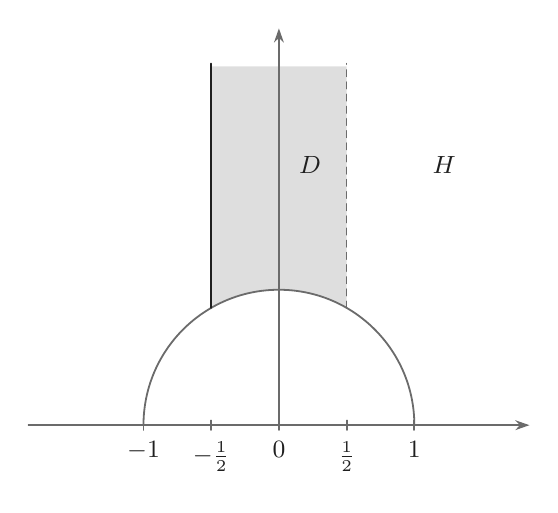
\begin{tikzpicture}[field/diagram, x=1.72cm, y=1.72cm]
    \fill[FieldRegion]
        (-0.5,2.65) -- (-0.5,{sqrt(3)/2})
        arc[start angle=120, end angle=60, radius=1]
        -- (0.5,2.65) -- cycle;
    \draw[field/axis] (-1.85,0) -- (1.85,0);
    \draw[field/axis] (0,0) -- (0,2.93);
    \draw[field/secondary] (-1,0)
        arc[start angle=180, end angle=0, radius=1];
    \draw[field/boundary] (-0.5,{sqrt(3)/2}) -- (-0.5,2.67);
    \draw[field/hidden] (0.5,{sqrt(3)/2}) -- (0.5,2.67);
    \foreach \x/\lab in {-1/{-1},-0.5/{-\frac12},0/{0},0.5/{\frac12},1/{1}} {
        \draw[field/secondary] (\x,-0.035) -- (\x,0.035);
        \node[below, inner sep=5pt] at (\x,0) {$\lab$};
    }
    \node[fill=FieldRegion, inner sep=2pt] at (0.23,1.92) {$D$};
    \node at (1.22,1.92) {$H$};
\end{tikzpicture}

        \FieldCaption{I}{7}{}
    \end{minipage}
\end{center}
\[
D=\left\{\tau\in H:\begin{array}{l}
\text{Either }-\tfrac12\leq\operatorname{Re}(\tau)<\tfrac12\text{ and }|\tau|>1\\
\text{or }|\tau|=1\text{ and }\operatorname{Re}(\tau)\leq0
\end{array}\right\}.
\]
It is clear from what we have said above that we can ``continuously deform'' complex structures on a real 2-dimensional torus to obtain an uncountable family of distinct complex structures. This is very characteristic: There may exist many different complex structures on a given differential manifold. The classification of all such structures is generally a problem of great difficulty and only partial results are known. For example, if $M$ is a compact Riemann surface of genus $g\geq2$, then it is known by the work of Riemann, Teichm\"uller \cite{bib:I:teichmuller-o:1}, Rauch \cite{bib:I:rauch-h-e:1}, Ahlfors \cite{bib:I:ahlfors-l-v:2} and Bers \cite{bib:I:bers-l:1} that the set of complex structures on $M$ has the natural structure of a complex analytic space of dimension $(3g-3)$. This space of complex structures---The moduli space\IndexMark{idx-398}{moduli space@Moduli space}---will have singularities. Unfortunately, no such global existence theorem holds in general for higher dimensional compact manifolds. One approach to a global theory is due to Griffiths \cite{bib:I:griffiths-p:1}. There is an infinitesimal theory of deformations of complex structure\IndexMark{idx-164}{deformation of complex structure@Deformation of complex structure} due to Kodaira, Spencer and Kuranishi. This is described in the book by Kodaira and Morrow \cite{bib:I:kodaira-k-and-morrow-j:1}. Finally we remark the difficult theorem of Douady's [1] to the effect that the set of all
% Original book page 155
complex analytic subspaces of a given complex analytic space has the natural structure of a complex analytic space.

We shall now briefly consider the question of the existence of meromorphic functions on a complex torus. First we look at 1-dimensional tori.

Let $\{\omega_1,\omega_2\}$ be a real basis of $\mathbb C$ and let $L$ denote the corresponding lattice. Set $T=\mathbb C/L$ and let $\pi:\mathbb C\longrightarrow T$ denote the quotient map. Given $a\in\mathbb C$, we let $P_a$ denote the parallelogram with vertices $a$, $a+\omega_1$, $a+\omega_2$, $a+\omega_1+\omega_2$. $P_a$ is called a \emph{period parallelogram}\IndexMark{idx-435}{period parallelogram@Period parallelogram} (for $L$) and obviously $\pi(P_a)=T$.

Suppose $m\in\mathcal M(T)$. Clearly $\widetilde m=m\pi\in\mathcal M(\mathbb C)$ and $\widetilde m$ is $L$-invariant. That is, given $z\in\mathbb C$,
\[
\widetilde m(z+\omega)=m(z),\quad\text{for all }\omega\in L.
\]
Equivalently, $\widetilde m$ is \emph{doubly periodic}\IndexMark{idx-212}{doubly periodic function@Doubly periodic function} with periods $\omega_1,\omega_2$,
\[
m(z+\omega_1)=m(z+\omega_2)=m(z),\quad\text{all }z\in\mathbb C.
\]
We shall say that an $L$-invariant meromorphic function\IndexMark{idx-389}{meromorphic function@Meromorphic function!on complex torus@on complex torus} on $\mathbb C$ or, equivalently, a meromorphic function on $T$, is ($L$-) \emph{elliptic}. Clearly the set of poles and zeroes of an elliptic function\IndexMark{idx-222}{elliptic function@Elliptic function} is finite (mod $L$).

\FieldHeading{Theorem}{4.4.2}{}\FieldTarget{theorem:4.4.2}{4.4.2} Let $m\in\mathcal M^*(T)$ and $\operatorname{div}(m)=\sum_{i=1}^k n_i\cdot z_i$. Then
\begin{enumerate}
\item $\displaystyle\sum_{i=1}^k\operatorname{residue}_{z_i}(m)=0$.
\item $\deg(\operatorname{div}(m))=0$.
\item $\displaystyle\sum_{i=1}^k n_iz_i=e$ (relative to the group law on $T$).
\end{enumerate}
\begin{proof}
Choose $a\in\mathbb C$ such that the boundary of the period parallelogram $P_a$ is disjoint from the poles and zeroes of $m$. 1 follows by integrating $m$ (strictly, $\widetilde m=\pi m$) round $\partial P_a$ and observing that the integrals along opposite sides cancel by the periodicity of $m$. Similarly 2 follows by integrating the elliptic function $m'/m$ round $\partial P_a$ (see also Lemma~\ref{lemma:1.4.2}). For 3 we integrate $zm'/m$ round $\partial P_a$. In this case the integrals round
% Original book page 156
opposite sides do not cancel but we do have
\[
(2\pi i)^{-1}\left\{\int_a^{a+\omega_1}-\int_{a+\omega_2}^{a+\omega_1+\omega_2}\frac{zm'}m\,dz\right\}
=-(2\pi i)^{-1}\omega_2\int_a^{a+\omega_1}\frac{m'}m\,dz.
\]
Now $(2\pi i)^{-1}\int_a^{a+\omega_1}m'/m\,dz$ is just the winding number of the closed curve $m([a,a+\omega_1])$ about zero and is therefore an integer, say $m_1$. Similarly for the other pair of boundary integrals. Lifting to $P_a$ and choosing $\widetilde z_i\in P_a$ such that $\pi(\widetilde z_i)=z_i$, $1\leq i\leq k$, we see that
\[
\sum_{i=1}^k n_i\widetilde z_i=m_2\omega_1-m_1\omega_2\in L.
\]
\end{proof}

\paragraph*{Remarks.} It follows from condition 1 of the Theorem that an elliptic function cannot have a single pole of order 1. The simplest possibilities are a single double pole with zero residue or two single poles with opposite residue. From condition 2 it follows that if $m\in\mathcal M^*(T)$, $c\in\mathbb C$, then $m$ and $m-c$ have the same number of zeroes. Hence the map $m:T\longrightarrow P^1(\mathbb C)$ (\hyperref[sec:1:4]{Chapter 1, \S4}, Example 1) takes all complex values the same number of times. Condition 3 gives a necessary condition on a divisor in order that it be the divisor of an elliptic function. It turns out that conditions 2 and 3 of the theorem are sufficient conditions on a divisor for it to be the divisor of a meromorphic function (Abel's Theorem).

We shall now construct some elliptic functions. We start by defining \emph{Weierstrass' elliptic function}\IndexMark{idx-652}{weierstrass elliptic function@Weierstrass elliptic function} $\wp(z)$:
\[
\wp(z)=z^{-2}+\sum{}'\big((z-\omega)^{-2}-\omega^{-2}\big),\qquad z\in\mathbb C\setminus L.
\]
Here the sum is over all $\omega\in L'=L\setminus\{0\}$. This sum is absolutely convergent at all points of $\mathbb C\setminus L$ and converges uniformly on compact subsets of $\mathbb C\setminus L$ (See the exercises at the end of this section and note that terms in the sum are $O(\omega^{-3})$). Hence $\wp\in\mathcal M(\mathbb C)$. Clearly $\wp$ is even: $\wp(-z)=\wp(z)$, $z\in\mathbb C\setminus L$. To show that $\wp$ is elliptic we consider the derivative $\wp'$. Now
\[
\wp'(z)=-2\sum(z-\omega)^{-3}
\]
is obviously elliptic and so, by integrating, we see that
% Original book page 157
\[
\wp(z+\omega)=\wp(z)+C(\omega),
\]
where $C(\omega)$ is independent of $z$. Since $\wp$ is even, $z=-\omega/2$ gives $C(\omega)=0$ and so $\wp$ is elliptic. Set
\[
G_j=\sum{}'\omega^{-2j},\qquad j\geq2.
\]
The reader may easily verify that the Laurent expansions of $\wp$ and $\wp'$ at zero are given by
\[
\begin{aligned}
\wp(z)&=z^{-2}\sum_{j\geq1}(2j+1)G_{2j+2}z^{2j},\\
\wp'(z)&=-2z^{-3}+\sum_{j\geq1}(2j+1)2jG_{2j+2}z^{2j-1}
\end{aligned}
\]
and converge for $0<|z|<\min_{L'}|\omega|$.

Let us find the divisor of $\wp'$. Since $\wp'$ is odd and $L$-invariant $\wp'(z)=0$ if $-z\equiv z\bmod L$. That is, if $2z\in L$. Thus representative zeroes of $\wp'$ in the period parallelogram $P_0$ are given by $\omega_1/2$, $\omega_2/2$, $(\omega_1+\omega_2)/2$. These are the only zeroes in $P_0$ by Theorem~\ref{theorem:4.4.2}. Now $\wp$ has only two zeroes in $P_0$ and, by condition 3 of Theorem~\ref{theorem:4.4.2} they must be $\{a,-a\}$ for some $a\in T$. These zeroes are not known explicitly in terms of the lattice $L$.

\FieldHeading{Proposition}{4.4.3}{}\FieldTarget{proposition:4.4.3}{4.4.3} The elliptic functions $\wp$ and $\wp'$ are related by the differential equation
\[
\wp'^2=4\wp^3-g_2\wp-g_3,
\]
where $g_2^3-27g_3^2\neq0$ and $g_2=60G_4$, $g_3=140G_6$.
\begin{proof}
$\wp'^2-4\wp^3$ is certainly elliptic. Using the Laurent series for $\wp$ and $\wp'$ we easily compute that
\[
\begin{aligned}
\wp'^2-4\wp^3&=-60G_4z^{-2}-140G_6+O(z^2)\\
&=-g_2\wp-g_3+h,
\end{aligned}
\]
where $h$ is holomorphic, elliptic and $O(z^2)$. Therefore $h\equiv0$.
% Original book page 158
Now we know the zeroes of $\wp'$ and so those of $4\wp^3-g_2\wp-g_3$. But the zeroes of $\wp'$ are distinct and so therefore are those of the cubic $4x^3-g_2x-g_3=0$. Therefore the discriminant of the cubic, $-16(g_2^3-27g_3^2)$, is non-zero.
\end{proof}

We have already indicated in the previous section that the cubic curve\IndexMark{idx-159}{cubic curve@Cubic curve} $y^2z-4x^3+g_2xz^2+g_3z^3=0$ is non-singular in $P^2(\mathbb C)$ provided that $g_2^3-27g_3^2\neq0$. The next theorem gives an explicit embedding of the torus\IndexMark{idx-467}{projective embedding@Projective embedding!of complex torus@of complex torus} $T$ as an algebraic submanifold of $P^2(\mathbb C)$.

\FieldHeading{Theorem}{4.4.4}{}\FieldTarget{theorem:4.4.4}{4.4.4}\IndexMark{idx-227}{embedding@Embedding!of complex 1 dimensional tori@of complex 1-dimensional tori} The mapping $\phi:T\longrightarrow P^2(\mathbb C)$ defined by
\[
\phi(z)=(z^3\wp(z),z^3\wp'(z),z^3)
\]
is a biholomorphic embedding of $T$ onto the cubic curve $y^2z-4x^3+g_2xz^2+g_3z^3=0$.
\begin{proof}
By Proposition~\ref{proposition:4.4.3}, $\phi$ maps $T$ into the given cubic curve. Certainly $\phi$ is onto since $\wp(z)=A$ has a solution for every $A\in P^1(\mathbb C)$ (remarks following Theorem~\ref{theorem:4.4.2}). $\phi$ is holomorphic since $z^3\wp(z)$ and $z^3\wp'(z)$ are holomorphic and the derivative of $\phi$ is everywhere of maximal rank as is seen by noting that $\wp''(z)\neq0$ if $z\in\{\omega_1/2,\omega_2/2,(\omega_1+\omega_2)/2\}$ as these points are simple zeroes of $\wp'$. It remains to be proved that $\phi$ is injective. Suppose $\wp(z)=\wp(y)$. If $z\not\equiv-z$, mod $L$, and $y\not\equiv z$, mod $L$, we see that $y\equiv-z$, mod $L$, since $\wp$ is even and takes each value twice (counting multiplicities). But $\wp'$ is odd and so $\wp'(z)\neq\wp'(y)$ unless $\wp'(z)=0$ which cannot happen as $z\not\equiv-z$, mod $L$. Now suppose $z\equiv-z$, mod $L$. Since $\wp$ takes each value twice, it is easy to see that $y\equiv-y$, mod $L$. But if $z\equiv-z$, mod $L$, $z\in\{\omega_1/2,\omega_2/2,(\omega_1+\omega_2)/2\}$. Now $\wp(\omega_1/2)$, $\wp(\omega_2/2)$, $\wp(\omega_1+\omega_2/2)$ are the roots of the cubic $4x^3-g_2x-g_3=0$ and are distinct by our assumption on the discriminant. Hence $z\equiv y$, mod $L$. Our argument proves that $\phi$ is injective.
\end{proof}

\paragraph*{Remarks.}
\begin{enumerate}
\item Here we have just given a tiny fragment of the theory of elliptic curves. The reader may consult Lang \cite{bib:I:lang-s:2}, Robert \cite{bib:I:robert-a:1} or Siegel \cite{bib:I:siegel-c-l:1} for more complete treatments of elliptic curves and functions. Whittaker and Watson \cite{bib:I:whittaker-e-t-and-watson-g-n:1} is a classical reference.
% Original book page 159
\item Although we have not proved it here, it is not difficult to show that every meromorphic function on a complex torus is a rational function of $\wp$ and $\wp'$. In particular, any two non-zero meromorphic functions are algebraically dependent (see also \hyperref[sec:5:9]{Chapter 5, \S9}).
\item It can be shown that any two meromorphic functions on a compact Riemann surface are algebraically dependent (see Gunning \cite[Theorem 26, \S10]{bib:I:gunning-r-c:1}). Consequently, we may generalise the method of proof of Theorem~\ref{theorem:4.4.4} to construct a holomorphic map of a compact Riemann surface $M$ onto an algebraic curve in $P^2(\mathbb C)$ provided that there exist ``sufficiently many'' meromorphic functions on $M$. The existence of an abundance of meromorphic functions on $M$ is a consequence of the Riemann--Roch theorem which we prove in Chapter 10 (see also \hyperref[sec:7:5]{\S5, Chapter 7}). In general, we cannot embed $M$ onto a non-singular curve in $P^2(\mathbb C)$ (we always can embed in $P^3(\mathbb C)$). We shall show in \hyperref[sec:7:5]{Chapter 7, \S5}, that every compact Riemann surface can be represented as a branched cover of $P^1(\mathbb C)$. In case the surface has genus $g>1$, and admits a 2-fold branched cover over $P^1(\mathbb C)$, the surface is called \emph{hyperelliptic}\IndexMark{idx-314}{hyperelliptic curve@Hyperelliptic curve}. We have more to say about these matters in Chapter 10. See also Griffiths and Harris \cite{bib:I:griffiths-p-and-harris-j:1}, Hartshorne \cite{bib:I:hartshorne-r:2} and Gunning \cite{bib:I:gunning-r-c:1}.
\end{enumerate}

For the remainder of this section we shall briefly consider complex tori of dimension $>1$.

We no longer have a good moduli space for $n$-dimensional complex tori if $n>1$. In fact the natural parameter space for complex structures on a real $2n$-dimensional torus turns out to be non-Hausdorff---see Kodaira and Spencer \cite[pages 408--414]{bib:I:kodaira-k-and-spencer-d-c:1} and also Kodaira and Morrow \cite[pages 22--23]{bib:I:kodaira-k-and-morrow-j:1}.

\FieldHeading{Definition}{4.4.5}{}\FieldTarget{definition:4.4.5}{4.4.5} A complex torus which is algebraic is called an \emph{Abelian variety}\IndexMark{idx-001}{abelian variety@Abelian variety}.

Every 1-dimensional complex torus is an Abelian variety (Theorem~\ref{theorem:4.4.4}). However, it is not the case that every $n$-dimensional complex torus is algebraic for $n>1$; in fact ``most'' are not. An obvious necessary condition for a complex torus to be algebraic is that it admit non-constant meromorphic functions (of course, we might expect to use such functions to construct maps into projective space). A stronger necessary condition is that we can separate points on the torus using meromorphic functions (since we can on projective space).
% Original book page 160
\paragraph*{Example 2. (Siegel \cite{bib:I:siegel-c-l:2}).} Let $T$ be the complex 2-dimensional torus whose lattice is generated by $\{(1,0),(0,1),i(\sqrt2,\sqrt3),i(\sqrt5,\sqrt7)\}\subset\mathbb C^2$. Then $T$ admits no nonconstant meromorphic functions. In particular, $T$ is not algebraic. We shall not prove this result here but instead refer the reader to Siegel \cite{bib:I:siegel-c-l:2}. See also Cornalba \cite[page 85]{bib:I:cornalba-m:1}, de La Harpe \cite[page 142]{bib:I:de-la-harpe-p:1}, Griffiths and Harris \cite{bib:I:griffiths-p-and-harris-j:1} and Swinnerton-Dyer \cite{bib:I:swinnerton-dyer-h-p-f:1}.

In fact in every dimension greater than 1 there exist complex tori with no non-constant meromorphic functions. We shall now give necessary and sufficient conditions for a complex torus $T$ with lattice $L$ generated by $\omega_1,\ldots,\omega_{2n}$ to be an Abelian variety.

Let $A:\mathbb C^n\times\mathbb C^n\longrightarrow\mathbb R$ be a real skew-symmetric bilinear form (that is, $A$ is real linear in each variable separately and $A(x,y)=-A(y,x)$). We say that $A$ is a \emph{Riemann form}\IndexMark{idx-526}{riemann form@Riemann form} for $T$ (or $L$) if
\begin{enumerate}
\item $A(L,L)\subset\mathbb Z$;
\item $A(ix,y)$ is a symmetric positive definite form on $\mathbb C^n$.
\end{enumerate}

\paragraph*{Example 3.} Every lattice $L\subset\mathbb C$ admits a Riemann form. Indeed, suppose that $L$ is generated by $\{\omega_1,\omega_2\}$ and that $\operatorname{Im}(\omega_1/\omega_2)>0$. Denote the area of the period parallelogram defined by $\omega_1,\omega_2$ by $S$. Clearly $S=\operatorname{Im}(\omega_1\bar\omega_2)$. If we define $A:\mathbb C\times\mathbb C\longrightarrow\mathbb R$ by $A(y,z)=S^{-1}\operatorname{Im}(y\bar z)$, then $A$ is a Riemann form for $L$. As an exercise the reader may verify that $A$ is the only Riemann form for $L$ which takes the values $\pm1$ on any basis of $L$.

For $n>1$, lattices do not generally admit a Riemann form or even a non-zero positive semi-definite form taking integer values on the lattice. However, it may be shown that the set of all lattices which admit a non-zero Riemann form is dense in the set of all lattices (obvious topology). If $A$ is a Riemann form for $L$ then we have a positive definite Hermitian form $H$ on $\mathbb C^n$ whose imaginary part is integer valued on the lattice. Indeed, we may define
\[
H(y,z)=A(iy,z)+iA(y,z),\qquad y,z\in\mathbb C^n.
\]
We have the fundamental result

\paragraph*{Theorem.} A complex torus is algebraic if and only if it admits a Riemann form.
% Original book page 161
We shall prove that the existence of a Riemann form implies that the torus is algebraic in \hyperref[sec:7:6]{\S6 of Chapter 7} (the converse is not difficult). The theorem will also follow from our results on compact K\"ahler manifolds presented in Chapter 10. The reader may also find proofs in Cornalba \cite{bib:I:cornalba-m:1}, Griffiths and Harris \cite{bib:I:griffiths-p-and-harris-j:1}, Swinnerton-Dyer \cite{bib:I:swinnerton-dyer-h-p-f:1} and Weil \cite{bib:I:weil-a:1}. These references also give further information and references about complex tori. In Chapter~\ref{ch:5} we shall have a little to say about the construction of meromorphic functions on complex tori as well as the role played by theta functions and holomorphic line bundles.

\subsection*{Exercises}
\begin{enumerate}
\item Show that if $L$ is a lattice in $\mathbb C$ then $\sum_{L\setminus\{0\}}|\omega|^{-\lambda}$ converges provided that $\lambda>2$. Deduce that the series for $\wp'(z)$ converges uniformly on compact subsets of $\mathbb C\setminus L$.
\item Let $L$ be a lattice in $\mathbb C$ and choose $\omega\in L\setminus\{0\}$ as close as possible to the origin. Show that there is a basis for $L$ which contains $\omega$.
\item Show that every even elliptic function may be written uniquely as a product $c\prod_{j=1}^k(\wp(u_j)-\wp(z))^{p_j}$, $c\in\mathbb C$ (You will need part 2 of Theorem~\ref{theorem:4.4.2}). By writing an elliptic function as the sum of an even elliptic function plus $\wp'\times{}$ even elliptic function, show that every elliptic function is a rational combination of $\wp$, $\wp'$ and that the field of elliptic functions is a quadratic extension of $\mathbb C(\wp)$ (Use Proposition~\ref{proposition:4.4.3}).
\item Let $F(x,y,z)$ be homogeneous of degree $d$ and $C\subset P^2(\mathbb C)$ denote the corresponding curve of degree $d$. Suppose $X\subset P^2(\mathbb C)$ is an elliptic curve parametrized by $(\wp(u),\wp'(u),1)$ as in Theorem~\ref{theorem:4.4.4}. Prove that the number of points of intersection of $X$ with $C$ (counting multiplicities) is $3d$ (This is a special case of B\'ezout's theorem.\par
Hint: Suppose $F(0,1,0)\neq0$. Consider the elliptic function $F(\wp,\wp',1)$ and apply Theorem~\ref{theorem:4.4.2}, part 2).
\item Suppose that the elliptic curve $X\subset P^2(\mathbb C)$ is parametrized by $(\wp,\wp',1)$. Show that the points $u,v,w\in X$ are collinear if and only if $u+v+w=e$ (relative to the group law on $X$). Deduce that
% Original book page 162
\[
\wp(u+v)=-\wp(u)-\wp(v)+\frac14\left(\frac{\wp'(u)-\wp'(v)}{\wp(u)-\wp(v)}\right)^2
\]
provided that $u\not\equiv\pm v\pmod L$, where $L$ is the lattice associated to $X$.
\item Use the methods of questions 4 and 5 to study the intersection of conics with a fixed elliptic curve in $P^2(\mathbb C)$.
\item Let the lattice $L\subset\mathbb C$ have basis $\{1,\tau\}$, $\operatorname{Im}(\tau)>0$. Show that the set of continuous homomorphisms of the torus $\mathbb C/L$ is in bijective correspondence with the set $M(L)$ of complex numbers $a$ such that $aL\subset L$. Clearly $M(L)\supset\mathbb Z$. Say that $\mathbb C/L$ has \emph{complex multiplication}\IndexMark{idx-108}{complex multiplication@Complex multiplication} if $M(L)$ is strictly bigger than $\mathbb Z$. Show that if $\mathbb C/L$ has complex multiplication then $\tau\in\mathbb Q(\sqrt{-p})$, for some positive integer $p$ and that $M(L)$ is then a subring of the ring of integers of the field $\mathbb Q(\sqrt{-p})$. Deduce that there are only countably many complex tori that admit complex multiplication.
\end{enumerate}

\section{Properly discontinuous actions}\IndexMark{idx-472}{properly discontinuous action@Properly discontinuous action}\label{sec:4:5}
Let $M$ be a complex manifold and $\operatorname{Aut}(M)$ denote the group of biholomorphic transformations of $M$. Denote the identity of $\operatorname{Aut}(M)$ by $I$. Suppose that $\Gamma$ is a subgroup of $\operatorname{Aut}(M)$. We say that $\Gamma$ acts \emph{freely} on $M$ if the only element of $\Gamma$ that has fixed points is the identity. That is, if $g\in\Gamma$ and $g(x)=x$ for some $x\in M$ then $g=I$. We say that $\Gamma$ acts \emph{properly discontinuously} on $M$ if for any pair $K_1,K_2$ of compact subsets of $M$, the set $\{g\in\Gamma:g(K_1)\cap K_2\neq\varnothing\}$ is finite.

\FieldHeading{Lemma}{4.5.1}{}\FieldTarget{lemma:4.5.1}{4.5.1} Let $\Gamma$ act freely, properly discontinuously on $M$. Then every point $x\in M$ has an open neighbourhood $U$ such that if $g\in\Gamma$ and $g(U)\cap U\neq\varnothing$, then $g=I$.
\begin{proof}
Let $V$ be any relatively compact open neighbourhood of $x$. Since $\Gamma$ acts properly discontinuously, $P=\{g\in\Gamma:g(V)\cap V\neq\varnothing\}$ is finite. Define
\[
U=V\setminus\bigcup_{g\in P\setminus\{I\}}g^{-1}\big(\overline{g(V)\cap V}\big).
\]
We leave it to the reader to check that $U$ satisfies the conditions of the lemma.
\end{proof}
% Original book page 163
\FieldHeading{Theorem}{4.5.2}{}\FieldTarget{theorem:4.5.2}{4.5.2} Let $M$ be a complex manifold and $\Gamma$ be a subgroup of $\operatorname{Aut}(M)$ which acts freely, properly discontinuously on $M$. Then there exists a natural complex structure on $M/\Gamma$ such that the orbit map $\pi:M\longrightarrow M/\Gamma$ is locally biholomorphic.
\begin{proof}
Let $y=\pi(x)\in M/\Gamma$. Choose a chart $(U,\phi)$ for $M$ containing $x$ such that the conditions of Lemma~\ref{lemma:4.5.1} hold for the open set $U$. $U$ is mapped homeomorphically onto $\pi(U)$ by $\pi$. Clearly $(\pi(U),\phi^{-1}(\pi|U)^{-1})$ is a chart on $M/\Gamma$ containing $y$. Repeating this construction for every point $y\in M/\Gamma$ we obtain a complex analytic atlas on $M/\Gamma$ relative to which $\pi$ is locally biholomorphic.
\end{proof}

\paragraph*{Examples.}
\paragraph*{1.} Let $M$ be a Riemann surface (not necessarily compact). Then, by the Uniformization theorem\IndexMark{idx-627}{uniformization theorem@Uniformization theorem}, the universal covering surface $\widetilde M$ of $M$ is biholomorphic to either the Riemann sphere, upper half plane (or open unit disc) or complex plane. Set $\Gamma=\pi_1(M)$. Then $\Gamma$ acts freely, properly discontinuously on $\widetilde M$ and $M$ is biholomorphic to $\widetilde M/\Gamma$. We remark that with the exception of the Riemann sphere, punctured complex plane, complex plane and torus, $\widetilde M$ is biholomorphic to the upper half plane. In this case $\Gamma$ is a discrete subgroup of the group of biholomorphic transformations of the upper half plane, $PSL(2,\mathbb R)$. ($PSL(2,\mathbb R)=SL(2,\mathbb R)/\{I,-I\}$ and acts on the upper half-plane by mapping $z\longmapsto(az+b)/(cz+d)$, $ad-bc=1$). Viewed in this light, the classification of Riemann surfaces amounts to the classification of all discrete subgroups of $PSL(2,\mathbb R)$.

\paragraph*{2.} Let $\Omega$ be a bounded domain\IndexMark{idx-053}{bounded domain@Bounded domain} in $\mathbb C^n$ and suppose that $\Gamma\subset\operatorname{Aut}(\Omega)$ acts freely, properly discontinuously on $\Omega$ and $\Omega/\Gamma$ is compact. Then $\Omega/\Gamma$ is algebraic. We prove this fundamental result of Kodaira \cite{bib:I:kodaira-k:1} in Chapter 10. We remark that it implies that if the universal cover of a compact complex manifold $M$ is biholomorphic to a bounded domain in $\mathbb C^n$ then $M$ is algebraic.

\paragraph*{3.} If $L\in\mathbb C^n$ is a lattice subgroup ($\cong\mathbb Z^{2n}$), then $L$ acts freely, properly discontinuously on $\mathbb C^n$ and so $\mathbb C^n/L$ has the structure of a complex manifold; see \hyperref[sec:4:4]{\S4} of this chapter.
% Original book page 164
\paragraph*{4.} Let $a_0,\ldots,a_n\in\mathbb C^*$ and suppose $|a_j|<1$, $0\leq j\leq n$. Let $\Gamma$ denote the cyclic subgroup of $\operatorname{Aut}(\mathbb C^{n+1}\setminus\{0\})$ generated by $g:(z_0,\ldots,z_n)\longmapsto(a_0z_0,\ldots,a_nz_n)$. Then $\Gamma$ acts freely, properly discontinuously on $\mathbb C^{n+1}\setminus\{0\}$ and so $(\mathbb C^{n+1}\setminus\{0\})/\Gamma$ has the structure of a complex manifold which is easily seen to be compact and diffeomorphic to $S^{2n+1}\times S^1$. Any complex manifold diffeomorphic to $S^{2n+1}\times S^1$ is called a \emph{Hopf manifold}\IndexMark{idx-311}{hopf@Hopf!manifold@manifold} and, if $n=1$, a \emph{Hopf surface}\IndexMark{idx-312}{hopf@Hopf!surface@surface}. As we shall see in Chapter 10, Hopf manifolds are never algebraic ($n\neq0$). Hopf surfaces have been studied in great detail by Kodaira \cite{bib:I:kodaira-k:2}. See also Kodaira and Spencer \cite{bib:I:kodaira-k-and-spencer-d-c:1} and Ueno \cite[pages 235--238]{bib:I:ueno-k:1}. Here we shall describe the important (and unpleasant!) phenomenon of ``jumping'' of complex structure\IndexMark{idx-344}{jumping of complex structure@Jumping of complex structure} that can occur on complex manifolds of dimension greater than one. Let $D$ denote the open unit disc in $\mathbb C$ and choose $a\in\mathbb C^*$, $|a|<1$. For $t\in D$, let $\Gamma_t$ be the subgroup of $\operatorname{Aut}(\mathbb C^2\setminus\{0\})$ generated by $g_t:(z_0,z_1)\longmapsto(az_0+z,az_1)$. Then $\Gamma_t$ acts freely, properly discontinuously on $\mathbb C^2\setminus\{0\}$ and so $M_t=(\mathbb C^2\setminus\{0\})/\Gamma_t$ has the structure of a complex manifold which is easily seen to be a Hopf surface. In this case, we may define $M=(\mathbb C^2\times\{0\})\times D/\Gamma$, where $\Gamma$ is generated by $g:((z_0,z_1),t)\longmapsto((az_0+tz_1,az_1),t)$. $M$ has the structure of a complex manifold and if we let $\pi:M\longrightarrow D$ denote the natural projection we see that $\pi$ is holomorphic and $\pi^{-1}(t)=M_t$, $t\in D$. Thus we have defined a complex analytic family of Hopf surfaces, parametrized by points in the unit disc. Suppose $f:M_t\longrightarrow M_s$ is biholomorphic, $t,s\in D$. Lift $f$ to the universal cover to obtain a biholomorphic map $F:\mathbb C^2\setminus\{0\}\longrightarrow\mathbb C^2\setminus\{0\}$ satisfying $Fg_t=g_sF$. By Hartog's theorem (Theorem~\ref{theorem:2.3.2}), $F$ extends to an analytic map $\bar F:\mathbb C^2\longrightarrow\mathbb C^2$ which is easily seen to be biholomorphic and to preserve the origin. Again we have $\bar Fg_t=g_s\bar F$. Differentiating this relation at zero we see that $D\bar F_0\cdot g_t=g_s\cdot D\bar F_0$. Setting $[D\bar F_0]=[F_{ij}]$, we easily compute that this relation implies that
\[
\begin{aligned}
tF_{00}z_1&=sF_{10}z_0+sF_{11}z_1,\\
tF_{10}z_1&=0.
\end{aligned}
\]
Hence if $st\neq0$, we must have $F_{10}=0$ and $tF_{00}=sF_{11}$. If these relations are satisfied, we see immediately that $DF_0$ induces a biholomorphic map between $M_t$ and $M_s$. That is, we have shown that the Hopf surfaces $M_t$ are all biholomorphic provided $t\neq0$. However, if say $s=0$, $t\neq0$, the
% Original book page 165
conditions above imply that $F_{00}=F_{10}=0$ and so $F$ cannot be biholomorphic. Therefore, $M_0$ is not biholomorphic to $M_t$, $t\neq0$. In other words the complex structure on $M_t$ ``jumps'' as $t$ passes through zero. Notice that although the analytic map $\pi:M\longrightarrow D$ is differentiably trivial it is \emph{not} analytically trivial.

\paragraph*{5. Calabi--Eckmann manifolds (Calabi and Eckmann \cite{bib:I:calabi-e-and-eckmann-b:1}).} Fix positive integers $p,q\geq0$ and consider the projection $\pi:S^{2p+1}\times S^{2q+1}\longrightarrow P^p(\mathbb C)\times P^q(\mathbb C)$ obtained as the product of the Hopf fibrations of $S^{2p+1}$ and $S^{2q+1}$. For each $x\in P^p(\mathbb C)\times P^q(\mathbb C)$, the fibre $\pi^{-1}(x)$ is diffeomorphic to a real two-dimensional torus and so admits a complex structure. Since the base carries a complex structure we might hope to be able to define a complex structure on the product $S^{2p+1}\times S^{2q+1}$ and we shall now show that this is possible.

Fix $\tau\in\mathbb C$, $\operatorname{Im}(\tau)>0$ and let $T_\tau$ denote the torus with lattice generated by $\{1,\tau\}$. Given integers $r,s$, $0\leq r\leq p$, $0\leq s\leq q$, define
\[
V_{rs}=\{((z_0,\ldots,z_p),(w_0,\ldots,w_q))\in S^{2p+1}\times S^{2q+1}:z_rw_s\neq0\}.
\]
$V_{rs}$ is an open subset of $S^{2p+1}\times S^{2q+1}$. We define a map $\phi_{rs}:V_{rs}\longrightarrow\mathbb C^{p+q}\times T_\tau$ by
\[
\begin{split}
\phi_{rs}((z_0,\ldots,z_p),(w_0,\ldots,w_q))={}&(z_0/z_r,\ldots,\widehat{z_r/z_r},\ldots,\\
&w_0/w_s,\ldots,\widehat{w_s/w_s},\ldots,t_{rs}),
\end{split}
\]
where
\[
t_{rs}=(2\pi i)^{-1}(\log(z_r)+\tau\log(w_s)),\quad\bmod1,\tau.
\]
It is a straightforward exercise to verify that $\phi_{rs}$ is a homeomorphism of $V_{rs}$ onto $\mathbb C^{p+q}\times T_\tau$ and that $\{(V_{rs},\phi_{rs}):0\leq r\leq p,\ 0\leq s\leq q\}$ defines a complex analytic structure on $S^{2p+1}\times S^{2q+1}$. Relative to this structure $\pi:S^{2p+1}\times S^{2q+1}\longrightarrow P^p(\mathbb C)\times P^q(\mathbb C)$ is holomorphic and the fibres of $\pi$ are biholomorphic to $T_\tau$. We call $S^{2p+1}\times S^{2q+1}$, with the complex structure defined above, a \emph{Calabi--Eckmann manifold}\IndexMark{idx-055}{calabi eckmann manifold@Calabi--Eckmann manifold}. Observe that if $P\in S^{2p+1}$, $Q\in S^{2q+1}$ then the complex manifold $X=(S^{2p+1}\setminus\{P\})\times(S^{2q+1}\setminus\{Q\})$ is homeomorphic to $\mathbb C^{p+q+1}$. However, the complex structure induced on $\mathbb C^{p+q+1}$ is quite different from the usual structure. We shall show that every analytic function on $X$ is constant. To see this, notice that if
% Original book page 166
$x\in P^p(\mathbb C)\times P^q(\mathbb C)$ then $(\pi|X)^{-1}(x)$ is biholomorphic to a complex torus provided that $\pi(P,Q)\neq x$. Such tori are dense in $X$ and if $f\in A(X)$, then certainly $f$ is constant on any of these tori (Proposition~\ref{proposition:4.2.4}). Hence, by continuity, $f$ is constant on any fibre $(\pi|X)^{-1}(x)$ and so induces a holomorphic function on $P^p(\mathbb C)\times P^q(\mathbb C)$ which must be constant. Alternatively, if we use Exercise 2, \hyperref[sec:2:2]{\S2, Chapter 2} (locally) we see that $f$ must extend to an analytic function on $S^{2p+1}\times S^{2q+1}$ and so $f$ must be constant. This example shows that a non-compact complex manifold which is homeomorphic to $\mathbb C^n$ need not be biholomorphic to any open subset of $\mathbb C^n$, $n\geq3$. This is in sharp contrast to what happens in case $n=1$.

\paragraph*{6. Exotic complex structures (Brieskorn and Van de Ven [1]).}\IndexMark{idx-245}{exotic complex structure@Exotic complex structure} Let $a=(a_0,\ldots,a_n)$ be an $(n+1)$-tuple of strictly positive integers. Let $X(a)\subset\mathbb C^{n+1}$ denote the zero set of the polynomial $z_0^{a_0}+\cdots+z_n^{a_n}$ and set $\Sigma(a)=X(a)\cap S^{2n+1}$. Now $X(a)\setminus\{0\}$ is a complex submanifold of $\mathbb C^{n+1}\setminus\{0\}$ and $\Sigma(a)$ is a differential submanifold of $S^{2n+1}$ (for the latter statement see Milnor \cite{bib:I:milnor-j-w:2}). If we let $\Gamma$ denote the cyclic subgroup of $\operatorname{Aut}(\mathbb C^{n+1}\setminus\{0\})$ generated by $g:(z_0,\ldots,z_n)\longmapsto(e^{1/a_0}z_0,\ldots,e^{1/a_n}z_n)$, then $\Gamma$ acts freely, properly discontinuously on $X(a)\setminus\{0\}$ and the resulting complex manifold $M=(X(a)\setminus\{0\})\setminus\Gamma$ is diffeomorphic to $S^1\times\Sigma(a)$. If one of the $a_j$'s equals one it is easy to see that $\Sigma(a)$ is diffeomorphic to $S^{2n-1}$ and so $M$ is a Hopf manifold. Suppose now that no $a_j$ is equal to one. Let $\xi_j=e^{2\pi i/a_j}$, $0\leq j\leq n$, and set
\[
\Delta(t)=\prod_{0<i_k<a_k}(t-\xi_0^{i_0}\cdots\xi_n^{i_n}).
\]
It is known (Brieskorn \cite{bib:I:brieskorn-e:1}) that if $n\neq2$ $\Sigma(a)$ is a homotopy $(2n-1)$-sphere if and only if $\Delta(1)=1$. Moreover, every homotopy $(2n-1)$-sphere $\Sigma^{2n-1}$ which bounds a parallelizable manifold is diffeomorphic to $\Sigma(a)$ for some $(n+1)$-tuple $a$ ($n\neq2$). For $n\geq4$, $\Sigma^{2n-1}$ is homeomorphic but not necessarily diffeomorphic to $S^{2n-1}$ (Brieskorn \cite{bib:I:brieskorn-e:1}, Milnor \cite{bib:I:milnor-j-w:3}). Now suppose $n\geq4$ and $a$ is chosen so that $\Sigma(a)$ is a homotopy sphere with non-standard differential structure. In Brieskorn and Van de Ven [1], it is shown that $S^1\times\Sigma(a)$ is not diffeomorphic to $S^1\times S^{2n-1}$ and so the resulting complex structure on $S^1\times\Sigma(a)$ is non-standard or ``exotic''. As a specific example, if we take $n=4$, $a_0=a_1=a_2=2$, $a_3=3$ and $a_4=6k-1$, it can be shown (see Brieskorn \cite{bib:I:brieskorn-e:1}) that as $k$ varies from 1 to 28 we obtain 28 distinct
% Original book page 167
complex structures on $S^1\times S^7$, 27 of which are exotic.

\subsection*{Exercises}
\begin{enumerate}
\item In the example describing Calabi--Eckmann manifolds show that if $p=0$, $q>0$, the resulting manifold is biholomorphic to a Hopf manifold.
\item Let $\Gamma$ be the subgroup of $GL(3,\mathbb C)$ consisting of matrices
\[
\begin{pmatrix}1&a_1&a_2\\0&1&a_3\\0&0&1\end{pmatrix},
\quad\text{where }a_j\in\mathbb Z[\sqrt{-1}]
\]
(that is, the $a_j$ are Gaussian integers).
Prove that $\Gamma$ acts freely, properly discontinuously on $\mathbb C^3$. The resulting complex manifold $\mathbb C^3/\Gamma$ is called an \emph{Iwasawa manifold}\IndexMark{idx-342}{iwasawa manifold@Iwasawa manifold}. Note that $\pi_1(\mathbb C^3/\Gamma)$ is not Abelian.
\end{enumerate}

\section{Analytic hypersurfaces}\label{sec:4:6}
In this section we make a global study of analytic sets defined locally by the vanishing of a single analytic function.

\FieldHeading{Definition}{4.6.1}{}\FieldTarget{definition:4.6.1}{4.6.1} Let $M$ be a complex manifold and $X$ be a proper analytic subset of $M$. We say that $X$ is an \emph{analytic hypersurface}\IndexMark{idx-018}{analytic hypersurface@Analytic hypersurface}\IndexMark{idx-321}{hypersurface@Hypersurface} of $M$ if for each $x\in X$ there exists $U\in\mathcal U_x$ and $f\in A(U)$ such that $X\cap U=f^{-1}(0)$.

Before stating the next Proposition we recall some notation from \hyperref[sec:3:5]{\S5 of Chapter 3}: Suppose $X$ is an analytic subset of $M$. As in \hyperref[sec:3:5]{\S5 of Chapter 3}, we may define the ideal $I_x(X)\lhd\mathcal O_x$ at each point $x\in M$. If $x\notin X$, $I_x(X)=\mathcal O_x$. Otherwise $I_x(X)$ is a non-trivial ideal of $\mathcal O_x$.

\FieldHeading{Proposition}{4.6.2}{}\FieldTarget{proposition:4.6.2}{4.6.2} Let $X$ be an analytic subset of the complex manifold $M$. The following conditions are equivalent.
\begin{enumerate}
\item $X$ is an analytic hypersurface.
\item For each $x\in X$, $I_x(X)$ is a principal ideal.
\end{enumerate}
\begin{proof}
Suppose $X$ is an analytic hypersurface and $x\in X$. Then there exists an open neighbourhood $U$ of $x$ and $f\in A(U)$ such that $f^{-1}(0)=X\cap U$. By the Nullstellensatz for principal ideals (Corollary~\ref{corollary:3.5.14}),
% Original book page 168
$I_x(X)=\operatorname{Rad}(f_x)$. But $f_x=\prod_{j=1}^k p_j^{r_j}$, where $p_j\in\mathcal O_x$ are irreducible and coprime. Hence $I_x(X)=(p_1\cdots p_k)$ and so is principal. For the converse, note that by Theorem~\ref{theorem:3.5.9} $Z(I_x(X))=X_x$. Therefore if $I_x(X)$ is principal, say $(f_x)$, we see that there exists an open neighbourhood $U$ of $x$ and representative $f\in A(U)$ of $f_x$ such that $X\cap U=f^{-1}(0)$.
\end{proof}

\FieldHeading{Definition}{4.6.3}{}\FieldTarget{definition:4.6.3}{4.6.3} Let $X$ be an analytic hypersurface in $M$ and $x\in X$. Suppose that $I_x(X)=(f_x)$ and that $df(x)\neq0$ for some representative $f$ of $f_x$. Then we say that $x$ is a \emph{regular} point of $X$. If $x$ is not regular we say it is a \emph{singular} point. We denote the set of regular and singular points\IndexMark{idx-504}{regular point of analytic set@Regular point of analytic set}\IndexMark{idx-575}{singular point of analytic set@Singular point of analytic set} of $X$ by $\operatorname{Reg}(X)$ and $\operatorname{Sing}(X)$ respectively.

\paragraph*{Remark.} A point $x\in X$ is a regular point of $X$ if and only if we can find an open neighbourhood $V$ of $x$ in $M$ such that $V\cap X$ is a complex submanifold of $M$. Indeed, if the latter condition holds we may find an open neighbourhood $W$ of $x$ contained in $V$ and $g\in A(W)$ such that $g^{-1}(0)=X\cap W$ and $dg(x)\neq0$. Since $dg(x)\neq0$ implies that $g_x$ is irreducible, we must have $I_x(X)=(g_x)$. The converse follows from the implicit function theorem.

\FieldHeading{Theorem}{4.6.4}{}\FieldTarget{theorem:4.6.4}{4.6.4} Let $X$ be an analytic hypersurface of the complex manifold $M$. We have
\begin{enumerate}
\item $\operatorname{Reg}(X)$ is an open and dense subset of $X$ and is a codimension one complex submanifold of $M$.
\item $\operatorname{Sing}(X)$ is an analytic subset of $M$.
\end{enumerate}
\begin{proof}
The remark above already shows that $\operatorname{Reg}(X)$ is an open subset of $X$ and a codimension one complex submanifold of $M$.

Let $x\in X$. By Theorem~\ref{theorem:3.5.16} we may find an open neighbourhood $V$ of $x$ in $M$ and $g\in A(V)$ such that $I_y(V)=(g_y)$, for all $y\in V$. Hence $\operatorname{Sing}(X)\cap V=\{y\in V:g(y)=dg(y)=0\}$. Hence $\operatorname{Sing}(X)$ is an analytic subset of $M$. Suppose that $\operatorname{Reg}(X)\cap V$ is not dense in $X\cap V$. Then for some $y\in X\cap V$, there exists an open neighbourhood $W$ of $y$ in $V$ such that $g(z)=dg(z)=0$, $z\in X\cap W$. Since $I_y(X)=(g_y)$, this implies that in a local coordinate system $(z_1,\ldots,z_n)$ at $y$ we would have
% Original book page 169
\[
(\partial g/\partial z_j)_y=u_y^jg_y,\qquad1\leq j\leq n,
\]
where $u_y^j\in\mathcal O_y$. However such a relation between an analytic function and its derivatives can only hold if the function is identically zero (look at Taylor series of $g$ and $dg$ at $y$). This contradiction shows that $\operatorname{Sing}(X)\cap V$ has no interior points in $X\cap V$. Therefore, $\operatorname{Reg}(X)$ is dense in $X$. Alternatively the reader may use the results at the beginning of \hyperref[sec:3:5]{\S5, Chapter 3} together with Corollary~\ref{corollary:3.5.15} to prove the density of $\operatorname{Reg}(X)$.
\end{proof}

The next result describes the local structure of an analytic hypersurface.

\FieldHeading{Proposition}{4.6.5}{}\FieldTarget{proposition:4.6.5}{4.6.5} Let $X$ be an analytic hypersurface in the complex manifold $M$ and let $x\in X$. We may find an open neighbourhood $U$ of $x$ in $M$ and analytic hypersurfaces $Z_j$, $j=1,\ldots,k$, in $U$ such that
\begin{enumerate}
\item $\displaystyle X\cap U=\bigcup_{j=1}^k Z_j$.
\item $\operatorname{Reg}(Z_j)$ is connected, $1\leq j\leq k$.
\item $\displaystyle\operatorname{Reg}(X)\cap U=\bigcup_{j=1}^k\left(\operatorname{Reg}(Z_j)\setminus\bigcup_{l\neq j}Z_l\right)$.
\end{enumerate}
\begin{proof}
Choose a chart $(U,\phi)$ for $M$ at $x$ such that $\phi(x)=0$. Set $D=\phi(U)$ and $Z=\phi(X\cap U)$. Since $\phi$ is biholomorphic, $Z$ is an analytic hypersurface in $D$. Shrinking $U$ if necessary, we may suppose (Corollary~\ref{corollary:3.5.15} and Theorem~\ref{theorem:3.5.16}) that $D$ is a polydisc and
\[
Z=\bigcup_{j=1}^k Z(p^j),
\]
where the $p^j$ are coprime, irreducible Weierstrass polynomials on $D$ and $I_y(Z)=(p_y^1\cdots p_y^k)$ for every $y\in D$. Set $Z_j=Z(p^j)$, $1\leq j\leq k$. Then $\operatorname{Reg}(Z_j)$ is a connected subset of $Z_j$, $1\leq j\leq k$ (Exercise 1, \hyperref[sec:3:5]{\S5, Chapter 3}). Since $I_y(Z)=(p_y^1\cdots p_y^k)$, $y\in D$, we see immediately that
\[
\operatorname{Reg}(Z)=\bigcup_{j=1}^k\left(\operatorname{Reg}(Z_j)\setminus\bigcup_{l\neq j}Z_l\right).
\]
Let $X_j$ denote the analytic hypersurface $\phi^{-1}(Z_j)$ in $D$, $1\leq j\leq k$. Clearly $\{X_j:1\leq j\leq k\}$ satisfy the conditions of the Proposition.
\end{proof}
% Original book page 170
\FieldHeading{Definition}{4.6.6}{}\FieldTarget{definition:4.6.6}{4.6.6} Let $X$ be an analytic subset of the complex manifold $M$. We say that $X$ is \emph{reducible} if we can find analytic subsets $Y,Z$ of $M$, neither of which equals $X$, such that $X=Y\cup Z$. If $X$ is not reducible, we say $X$ is \emph{irreducible}\IndexMark{idx-335}{irreducible@Irreducible!analytic set@analytic set}.

\FieldHeading{Theorem}{4.6.7}{}\FieldTarget{theorem:4.6.7}{4.6.7} Let $X$ be an analytic hypersurface of the complex manifold $M$ and $\{X'_i:i\in I\}$ denote the set of connected components of $\operatorname{Reg}(X)$. Set\IndexMark{idx-502}{reducible analytic set@Reducible analytic set} $X_i=\overline{X'_i}$, $i\in I$. Then
\begin{enumerate}
\item $X_i$ is an irreducible analytic hypersurface, $i\in I$.
\item $\{X_i:i\in I\}$ is locally finite. In particular, if $M$ is compact $I$ is finite.
\item $X=\bigcup_{i\in I}X_i$ and this decomposition of $X$ as a (countable) union of irreducible analytic hypersurfaces is unique up to order.
\item If $Y$ is any proper irreducible analytic subset of $M$ and $Y\subset X$ then $Y\subset X_i$ for some $i\in I$.
\end{enumerate}
\begin{proof}
Let $x\in X$ and suppose $x\in X_i$. We can find an open neighbourhood $U$ of $x$ in $M$ and hypersurfaces $Z_j$, $1\leq j\leq k$, in $U$ satisfying the conditions of Proposition~\ref{proposition:4.6.5}. Define
\[
R_j=\operatorname{Reg}(Z_j)\setminus\bigcup_{l\neq j}Z_l.
\]
For $1\leq j\leq k$, $R_j\subset\operatorname{Reg}(X)$ and is connected. Hence for some subset $\Lambda\subset\{1,\ldots,k\}$, $R_j\subset X'_i$ if and only if $j\in\Lambda$. But now $X_i\cap U=\bigcup_{j\in\Lambda}\bar R_j=\bigcup_{j\in\Lambda}Z_j$. This proves that $X_i$ is an analytic hypersurface in $M$. Since only finitely many of the $X_i$ can meet $U$, the family $\{X_i:i\in I\}$ is locally finite. Next we show that each $X_i$ is irreducible. Suppose that $X_i=Y\cup Z$, where $Y$ and $Z$ are analytic subsets of $M$. Set $Y'=X'_i\cap Y$, $Z'=X'_i\cap Z$. Since $X'_i$ is a complex submanifold we see that $Y',Z'$ are analytic subsets of $X'_i$. Now $Y',Z'$ cannot both be proper analytic subsets of $X'_i$ since if they were they would be nowhere dense in $X'_i$ (Corollary~\ref{corollary:2.2.3}) and so $X'_i$ could not be the union of $Y'$ and $Z'$. Suppose then that $Y'=X'_i$. Taking closures we see that $Y=X_i$ and so $X_i$ is irreducible.
% Original book page 171
Finally suppose that $Y$ is an irreducible analytic subset and $Y\subset X$. Setting $Y_i=X_i\cap Y$, we have $Y=\bigcup_{i\in I}Y_i$. Fix $y\in Y$ and let $L$ be the finite subset of $I$ characterised by $j\in L$ if and only if $y\in X_j$. Since $\{X_i:i\in I\}$ is locally finite, $\Sigma=\bigcup_{i\in I\setminus L}Y_i$ is an analytic subset of $M$. Clearly $\Sigma\neq Y$, since $y\notin\Sigma$. But now we have expressed $Y$ as a finite union
\[
Y=\bigcup_{i\in L}Y_i\cup\Sigma
\]
of analytic sets. Since $\Sigma\neq Y$, we must have $Y=Y_i$ for some $i\in L$. That is $Y\subset X_i$.
\end{proof}

As an immediate corollary of Theorem~\ref{theorem:4.6.7} we have

\FieldHeading{Theorem}{4.6.8}{}\FieldTarget{theorem:4.6.8}{4.6.8} An analytic hypersurface is irreducible if and only if its set of regular points is connected.

\paragraph*{Remarks.}
\begin{enumerate}
\item We call the hypersurfaces $X_i$ constructed in Theorem~\ref{theorem:4.6.7} the \emph{irreducible components}\IndexMark{idx-336}{irreducible@Irreducible!components@components} of $X$.
\item Theorems~\ref{theorem:4.6.7} and \ref{theorem:4.6.8} hold for arbitrary analytic subsets of a complex manifold. For proofs and further details we refer the reader to Gunning and Rossi \cite{bib:I:gunning-r-c-and-rossi-h:1}, R. Narasimhan \cite{bib:I:narasimhan-r:3} and Whitney \cite{bib:I:whitney-h:1}.
\item Notice that if $X$ is an irreducible analytic hypersurface it does not follow that $X_x$ is irreducible at every point $x\in X$. For example, the hypersurface $y^2=x^2(1-x)$ is irreducible but its germ at the origin is reducible.
\item Theorems~\ref{theorem:4.6.7} and \ref{theorem:4.6.8} do not generalise to real analytic sets. For example, $y^2=x^3$ is irreducible in $\mathbb R^2$ but the set of regular points is not connected. See R. Narasimhan \cite[Chapter V]{bib:I:narasimhan-r:3} for further examples of the pathology that can occur with real analytic sets.
\end{enumerate}
In \hyperref[sec:4:2]{\S2}, 4 of Chapter~\ref{ch:1} we defined and discussed divisors on a Riemann surface and their relationship to meromorphic functions. For the remainder of this section we shall show how we may use Theorem~\ref{theorem:4.6.7} to
% Original book page 172
give a local description of divisors on an arbitrary complex manifold\IndexMark{idx-195}{divisors@Divisors!on compact complex manifolds@on compact complex manifolds}.

\FieldHeading{Definition}{4.6.8}{}\FieldTarget{definition:4.6.8}{4.6.8} Let $M$ be a complex manifold. A \emph{Weil divisor}\IndexMark{idx-182}{divisor@Divisor}\IndexMark{idx-184}{divisor@Divisor!weil@Weil}\IndexMark{idx-657}{weil divisor@Weil divisor} on $M$ is a formal sum $\sum_{i\in I}n_i\cdot X_i$, where $\{X_i:i\in I\}$ is a locally finite set of mutually distinct irreducible analytic hypersurfaces in $M$ and $n_i\in\mathbb Z$, $i\in I$.

As in Chapter~\ref{ch:1}, we denote the set of Weil divisors on $M$ by $\mathcal D(M)$ and note that $\mathcal D(M)$ has the structure of an ordered Abelian group. If $d=\sum_{i\in I}n_i\cdot X_i\in\mathcal D(M)$, we let $|d|$ denote the analytic hypersurface $\bigcup_{i\in I}X_i$.

\paragraph*{Example 1.} Let $X$ be a non-singular analytic hypersurface in $P^n(\mathbb C)$. Assuming Chow's theorem, we see that $X$ is algebraic and so is the zero set of a homogeneous polynomial $P$. Since $X$ is non-singular, $X$ is (analytically) irreducible and it is not hard to verify that $P$ can be chosen to be irreducible (as a polynomial). Let $d=\operatorname{degree}(P)$. We say that $X$ is a \emph{hypersurface of degree $d$}\IndexMark{idx-323}{hypersurface@Hypersurface!of degree d@of degree $d$}. Now suppose $d>1$. Let $P^n(\mathbb C)^*$ denote the set of hyperplanes in $P^n(\mathbb C)$ (see also \hyperref[sec:4:4]{\S4}). Every hyperplane $H\in P^n(\mathbb C)^*$ will intersect $X$ in a Weil divisor. Indeed, changing coordinates we may assume that $H$ is the hyperplane $z_0=0$. $H\cap X$ is then the algebraic set determined by $G(z_1,\ldots,z_n)=P(0,z_1,\ldots,z_n)=0$. $G$ may not be irreducible and we let
\[
G(z_1,\ldots,z_n)=\prod_{i=1}^qG_i(z_1,\ldots,z_n)^{n_i}
\]
denote the prime factorization of $G$. If we set $X_i=G_i^{-1}(0)\cap H$, we see that $X\cap H$ determines the divisor
\[
d(X\cap H)=\sum_{i=1}^qn_i\cdot X_i.
\]
Notice that $\sum_{i=1}^qn_id_i=d$, where $d_i=\operatorname{degree}(G_i)$, $1\leq i\leq q$. Let $\Gamma=\{d(X\cap H):H\in P^n(\mathbb C)^*\}\subset\mathcal D(X)$. $\Gamma$ is in bijective correspondence with $P^n(\mathbb C)^*$. Given $d\in\Gamma$, we let $H(d)\in P^n(\mathbb C)^*$ denote the corresponding hyperplane. The set of divisors $\Gamma$ on $X$ determines the embedding of $X$ in $P^n(\mathbb C)$. Indeed, if $x\in X$ let $\Gamma_x$ denote the set of all divisors $d\in\Gamma$ such
% Original book page 173
that $x\in|d|$. Define $\phi(x)\in P^n(\mathbb C)$ to be $\bigcap_{d\in\Gamma_x}H(d)$. The reader may easily verify that $\phi$ embeds $X$ in $P^n(\mathbb C)$. As we shall see later there is a close relationship between families of divisors on compact complex manifolds\IndexMark{idx-196}{divisors@Divisors!on compact complex manifolds@on compact complex manifolds} and embeddings into projective space.

Our next definition is motivated by the Cousin II problem\IndexMark{idx-152}{cousin problems@Cousin problems} and the question of constructing a meromorphic function with specified pole and zero set with multiplicities.

\FieldHeading{Definition}{4.6.9}{}\FieldTarget{definition:4.6.9}{4.6.9} A \emph{Cartier divisor}\IndexMark{idx-065}{cartier divisor@Cartier divisor}\IndexMark{idx-183}{divisor@Divisor!cartier@Cartier} $d$ on the complex manifold $M$ consists of an open cover $\{U_i:i\in I\}$ of $M$ together with meromorphic functions $m_i\in\mathcal M^*(U_i)$ such that for all $i,j\in I$ we have $m_im_j^{-1}\in A^*(U_{ij})$. We write $d=\{(U_i,m_i):i\in I\}$.

\paragraph*{Remarks.}
\begin{enumerate}
\item We regard the Cartier divisors $d=\{(U_i,m_i):i\in I\}$, $d'=\{(V_j,m'_j):j\in J\}$ as being equal if $m'_jm_i^{-1}\in A^*(V_j\cap U_i)$, $i\in I$, $j\in J$. That is, we think of a Cartier divisor as an equivalence class of local data. Later, in Chapter~\ref{ch:6}, we shall give a slicker definition of Cartier divisor in terms of sheaves.
\item We let $\widetilde{\mathcal D}(M)$ denote the set of Cartier divisors on $M$.
\item Of course, a Cartier divisor is nothing else than the data for the Cousin II problem (Definition~\ref{definition:3.4.10}). However, we prefer to reserve the term ``Cousin II problem'' for non-compact complex manifolds, especially domains of holomorphy and Stein manifolds.
\end{enumerate}

\FieldHeading{Proposition}{4.6.10}{}\FieldTarget{proposition:4.6.10}{4.6.10} The set of Cartier divisors $\widetilde{\mathcal D}(M)$ has the natural structure of an Abelian group.
\begin{proof}
Let $d=\{(U_i,m_i):i\in I\}$, $d'=\{(V_j,m'_j):j\in J\}\in\widetilde{\mathcal D}(M)$. We define
\[
\begin{aligned}
d+d'&=\{(U_i\cap V_j,m_im'_j):i\in I,\ j\in J\},\\
-d&=\{(U_i,m_i^{-1}):i\in I\}.
\end{aligned}
\]
% Original book page 174
It is straightforward to verify that these definitions do not depend on the particular choice of local data for the divisors.
\end{proof}

\paragraph*{Example 2.} We have a natural group homomorphism $\operatorname{div}:\mathcal M^*(M)\longrightarrow\widetilde{\mathcal D}(M)$ defined by $\operatorname{div}(m)=\{(M,m)\}\in\widetilde{\mathcal D}(M)$. $\operatorname{div}(m)$ is called the \emph{divisor} of $m$.

\FieldHeading{Theorem}{4.6.11}{}\FieldTarget{theorem:4.6.11}{4.6.11} There is a natural group isomorphism between $\mathcal D(M)$ and $\widetilde{\mathcal D}(M)$.
\begin{proof}
Let $d=\sum_{i\in I}n_i\cdot X_i\in\mathcal D(M)$. Given $x\in M$, choose an open neighbourhood $U_x$ of $x$ and $p^i\in A(U_x)$, $i\in I$, such that
\begin{enumerate}
\item[a)] All but finitely many of the $p^i$ are identically equal to 1.
\item[b)] $I_y(X_i)=(p_y^i)$, $y\in U_x$, $i\in I$.
\end{enumerate}
Set
\[
m_x=\prod_{i\in I}(p^i)^{n_i}\in\mathcal M^*(U_x).
\]
Clearly $\phi(d)=\{(U_x,m_x):x\in M\}$ is a Cartier divisor on $M$. The map\IndexMark{idx-186}{divisor class map@Divisor class map} $\phi:\mathcal D(M)\longrightarrow\widetilde{\mathcal D}(M)$ is easily seen to be an injective group homomorphism.

Conversely, suppose $d=\{(U_i,m_i):i\in I\}$ is a Cartier divisor on $M$. Define $X=\bigcup_{i\in I}(Z(m_i)\cup P(m_i))$. $X$ is a well defined analytic hypersurface in $M$. Indeed, $X\cap U_i=Z(m_i)\cup P(m_i)$ since the condition $m_im_j^{-1}\in A^*(U_{ij})$ implies that $m_i$ and $m_j$ have the same pole and zero sets on $U_{ij}$. Let $\{X_\alpha:\alpha\in\Lambda\}$ be the decomposition of $X$ into its irreducible components. Refining the cover $\{U_i:i\in I\}$ if necessary, we may find for each $i\in I$, $p_\alpha\in A(U_i)$ such that
\begin{enumerate}
\item[a)] All but finitely many of the $p_\alpha$ are identically equal to 1.
\item[b)] $U_i\cap X_\alpha=p_\alpha^{-1}(0)$, $\alpha\in\Lambda$.
\item[c)] $I_y(X_\alpha)=(p_{\alpha,y})$, $y\in U_i$, $\alpha\in\Lambda$.
\end{enumerate}
Given $y\in U_i$, we see that there exist a unit $u_y\in\mathcal O_y$ and integers $n_\alpha$, $\alpha\in\Lambda$, such that
\[
m_y=u_y\prod_{\alpha\in\Lambda}p_{\alpha,y}^{n_\alpha}.
\]
% Original book page 175
Hence for some $u\in A^*(U_i)$, we have $m_i=u\prod_{\alpha\in\Lambda}p_\alpha^{n_\alpha}$. (We assume here that $U_i$ is connected, otherwise we could only claim that the $n_\alpha$ were constant on connected components of $U_i$).

We claim that the integers $n_\alpha$ do not depend on $i\in I$. This follows since $n_\alpha$ is constant on the connected open set $\operatorname{Reg}(X_\alpha)\cap\operatorname{Reg}(X)$. Since $\operatorname{Reg}(X_\alpha)\cap\operatorname{Reg}(X)$ is dense in $X_\alpha$, $n_\alpha$ is constant on $X_\alpha$. We now define
\[
\gamma(d)=\sum_{\alpha\in\Lambda}n_\alpha\cdot X_\alpha\in\mathcal D(M).
\]
By our construction it is clear that $\gamma=\phi^{-1}$ and so $\mathcal D(M)$ and $\widetilde{\mathcal D}(M)$ are naturally isomorphic.
\end{proof}

\paragraph*{Remarks.}
\begin{enumerate}
\item In the sequel we regard $\mathcal D(M)$ and $\widetilde{\mathcal D}(M)$ as identified by the isomorphism constructed above and write $\mathcal D(M)$ for the set of divisors on $M$, omitting the prefix ``Weil'' or ``Cartier''.
\item If we attempt to define divisors on more general objects, such as analytic sets with singularities, we find that the sets of Weil and Cartier divisors need not agree and in practice we tend to work with the less geometrical Cartier divisors (see Hartshorne \cite[pages 140--142]{bib:I:hartshorne-r:2}).
\end{enumerate}

\paragraph*{Example 3.}\IndexMark{idx-501}{rational function@Rational function!on projective space@on projective space} Let $m\in\mathcal M^*(P^n(\mathbb C))$. Then $\operatorname{div}(m)=\sum_{i=1}^qn_i\cdot X_i$, where the $X_i$ are irreducible analytic hypersurfaces in $P^n(\mathbb C)$. By Chow's theorem and Example 1, each $X_i$ is an irreducible algebraic hypersurface of degree $d_i$, say. Suppose that $X_i$ is the zero locus of the irreducible homogeneous polynomial $P_i$ of degree $d_i$, $1\leq i\leq q$. Define $R=\prod_{i=1}^qP_i^{n_i}$. Regarding $m$ and $R$ as defining meromorphic functions on $\mathbb C^{n+1}\setminus\{0\}$, we clearly have $\operatorname{div}(m)=\operatorname{div}(R)$ and so $\operatorname{div}(R^{-1}m)=0$. But therefore $R^{-1}m$ is an analytic function on $\mathbb C^{n+1}\setminus\{0\}$ and so extends by Hartog's theorem to an analytic function on the whole of $\mathbb C^{n+1}$. Taking the Taylor expansion of $R^{-1}m$ at 0 and noting that $m$ is homogeneous of degree zero, we see that $R^{-1}m$ is a homogeneous polynomial of degree $-\sum_{i=1}^qn_id_i$. Hence $\sum_{i=1}^qn_id_i=0$
% Original book page 176
(otherwise $\operatorname{div}(R^{-1}m)$ could not vanish). Consequently, $R^{-1}m=c$, for some $c\in\mathbb C^*$ and so
\[
m=c\prod_{i=1}^qP_i^{n_i}\quad\text{on }P^n(\mathbb C).
\]
We have shown that every meromorphic function on $P^n(\mathbb C)$ is rational. Our arguments further prove that a divisor $d=\sum_{i=1}^qn_i\cdot X_i$ on $P^n(\mathbb C)$ is the divisor of a meromorphic (rational) function on $P^n(\mathbb C)$ if and only if $\sum_{i=1}^qn_id_i=0$, where $d_i$ is the degree of the hypersurface $X_i$. Given $d=\sum_{i=1}^qn_i\cdot X_i\in\mathcal D(P^n(\mathbb C))$, we may define the degree of $d$, $\deg(d)$, to be the sum $\sum_{i=1}^qn_id_i$, where $d_i$ is the degree of the hypersurface $X_i$. Degree defines a homomorphism $\deg:\mathcal D(P^n(\mathbb C))\longrightarrow\mathbb Z$ and the kernel of the degree map is precisely the set of divisors of rational functions on $P^n(\mathbb C)$. (For an alternative proof of the rationality of meromorphic functions on $P^n(\mathbb C)$, avoiding the use of Chow's theorem, see Jackson \cite{bib:I:jackson-d:1}).

\section{Blowing up}\label{sec:4:7}
In this section we describe an operation on complex manifolds that is of the greatest importance in the study of singularities of analytic sets and the classification theory of complex manifolds.

Let $\Sigma\subset\mathbb C^n\times P^{n-1}(\mathbb C)$ be the set of points $((z_1,\ldots,z_n),(\zeta_1,\ldots,\zeta_n))$ satisfying the equations
\[
z_i\zeta_j=z_j\zeta_i,\qquad1\leq i,j\leq n.
\]
(We suppose in what follows that $n\geq2$). Notice that $((z_1,\ldots,z_n),(tz_1,\ldots,tz_n))\in\Sigma$, for all $(z_1,\ldots,z_n)\neq0$ and $t\in\mathbb C^*$. In other words, given $X\in\mathbb C^n$, $X\neq0$, $\Sigma$ contains the point corresponding to $X$ and the line through $X$. Since $\{0\}\times P^{n-1}(\mathbb C)\subset\Sigma$, we see that $\Sigma$ contains the point corresponding to zero and all the lines through zero. The reader may easily verify that we have described all the points in $\Sigma$. Let $\pi:\Sigma\longrightarrow\mathbb C^n$ denote the restriction of the projection of $\mathbb C^n\times P^{n-1}(\mathbb C)$ on $\mathbb C^n$ to $\Sigma$. If we set $E=\pi^{-1}(0)$, then $E$ is biholomorphic to $P^{n-1}(\mathbb C)$ and $\pi$
% Original book page 177
maps $\Sigma\setminus E$ bijectively onto $\mathbb C^n\setminus\{0\}$. We call $\Sigma$ the \emph{blowing up}\IndexMark{idx-050}{blowing up@Blowing-up} of $\mathbb C^n$ at 0. Amongst many other commonly used terms to describe $\Sigma$ are: $\mathbb C^n$ blown up at zero; the \emph{quadratic transform}\IndexMark{idx-496}{quadratic transform@Quadratic transform} of $\mathbb C^n$ at zero; the \emph{monoidal transform}\IndexMark{idx-401}{monoidal transform@Monoidal transform} of $\mathbb C^n$ at zero; the \emph{Hopf $\sigma$-process}\IndexMark{idx-313}{hopf process@Hopf $\sigma$-process} of $\mathbb C^n$ at zero. We call 0 the \emph{centre}\IndexMark{idx-075}{centre of blowing up@Centre (of blowing up)} of the blowing up; $E$ is called the \emph{exceptional variety}\IndexMark{idx-242}{exceptional variety@Exceptional variety}.

It is easy to see that $\Sigma$ is a complex submanifold of $\mathbb C^n\times P^{n-1}(\mathbb C)$ and we shall now construct an explicit atlas for $\Sigma$. For $1\leq j\leq n$, define $\gamma_j:\mathbb C^n\longrightarrow\Sigma\subset\mathbb C^n\times P^{n-1}(\mathbb C)$ by
\[
\begin{split}
\gamma_j(X_1,\ldots,X_n)=\big(& (X_1X_j,\ldots,X_{j-1}X_j,X_j,X_{j+1}X_j,\ldots,X_nX_j),\\
&(X_1,\ldots,X_{j-1},1,\ldots,X_n)\big).
\end{split}
\]
The reader may verify that $\gamma_j$ maps $\mathbb C^n$ homeomorphically onto an open subset of $\Sigma$. If we set $U_j=\gamma_j(\mathbb C^n)$, $\phi_j=\gamma_j^{-1}$, then $\{(U_j,\phi_j):1\leq j\leq n\}$ is a complex analytic atlas on $\Sigma$. Relative to this complex structure on $\Sigma$, $\pi:\Sigma\longrightarrow\mathbb C^n$ is holomorphic and $\pi$ maps $\Sigma\setminus E$ biholomorphically onto $\mathbb C^n\setminus\{0\}$.

\begin{center}
    \begin{minipage}{\linewidth}
        \centering
        % Figure 8. Gray distinguishes the cone S from the surrounding plane.
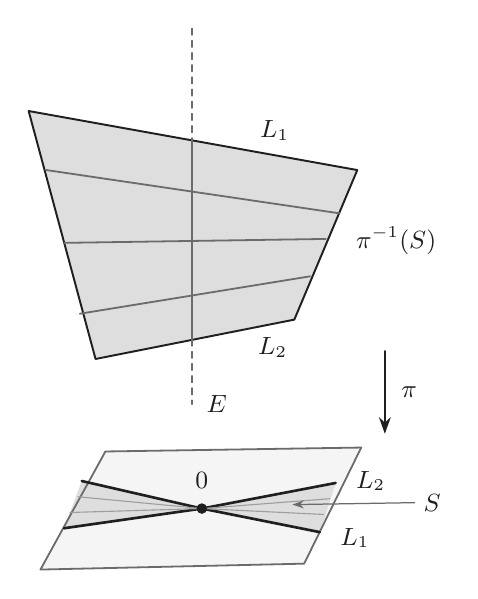
\begin{tikzpicture}[field/diagram, x=0.025cm, y=0.025cm]
    \fill[FieldRegion] (42,243) -- (209,213) -- (177,137) -- (76,117) -- cycle;
    \draw[field/boundary] (42,243) -- (209,213) -- (177,137) -- (76,117) -- cycle;
    \draw[field/secondary] (51,213) -- (200,191)
                           (60,176) -- (193,178)
                           (68,140) -- (185,159);
    \draw[field/hidden] (125,285) -- (125,228)
                        (125,127) -- (125,94);
    \draw[field/secondary] (125,228) -- (125,127);
    \node[above, inner sep=4pt] at (167,221) {$L_1$};
    \node[below, inner sep=4pt] at (166,135) {$L_2$};
    \node[right, inner sep=5pt] at (200,177) {$\pi^{-1}(S)$};
    \node[right] at (128,94) {$E$};
    \draw[field/map] (223,121) -- (223,79)
        node[midway, right, inner sep=5pt] {$\pi$};

    \fill[FieldPaper] (48,10) -- (81,70) -- (211,72) -- (182,13) -- cycle;
    \fill[FieldRegion] (60,31) -- (69,55) -- (130,41) -- cycle;
    \fill[FieldRegion] (198,54) -- (190,29) -- (130,41) -- cycle;
    \draw[field/secondary] (48,10) -- (81,70) -- (211,72) -- (182,13) -- cycle;
    \draw[field/curve] (60,31) -- (130,41) -- (198,54)
                       (69,55) -- (130,41) -- (190,29);
    \draw[field/guide] (63,39) -- (130,41) -- (195,46)
                       (67,47) -- (130,41) -- (192,38);
    \node[field/point] at (130,41) {};
    \node[above, inner sep=4pt] at (130,44) {$0$};
    \node[right, inner sep=5pt] at (200,55) {$L_2$};
    \node[right, inner sep=5pt] at (192,26) {$L_1$};
    \node (S) at (247,44) {$S$};
    \draw[field/leader] (S.west) -- (176,43);
\end{tikzpicture}

        \FieldCaption{I}{8}{\quad\emph{Blowing up}}
    \end{minipage}
\end{center}
% Original book page 178
In the figure the cone $S\subset\mathbb C^n$ is blown up into an open subset of $\Sigma$. That is, the cone is ``untwisted'' into an open set. Notice how lines passing through the origin of $\mathbb C^n$ lift to distinct lines in $\Sigma$. We can also describe this phenomenon using charts of the atlas we constructed above for $\Sigma$. Thus if $n=2$ and we take any open cone $S\subset\mathbb C^2$ which contains the $z_1$-axis but omits the $z_2$-axis then $\pi^{-1}(S)$ is described by the figure below if we use coordinates given by the chart $(U_1,\phi_1)$.

\begin{center}
    \begin{minipage}{\linewidth}
        \centering
        % Figure 9. Corresponding horizontal line and line through the blow-up centre.
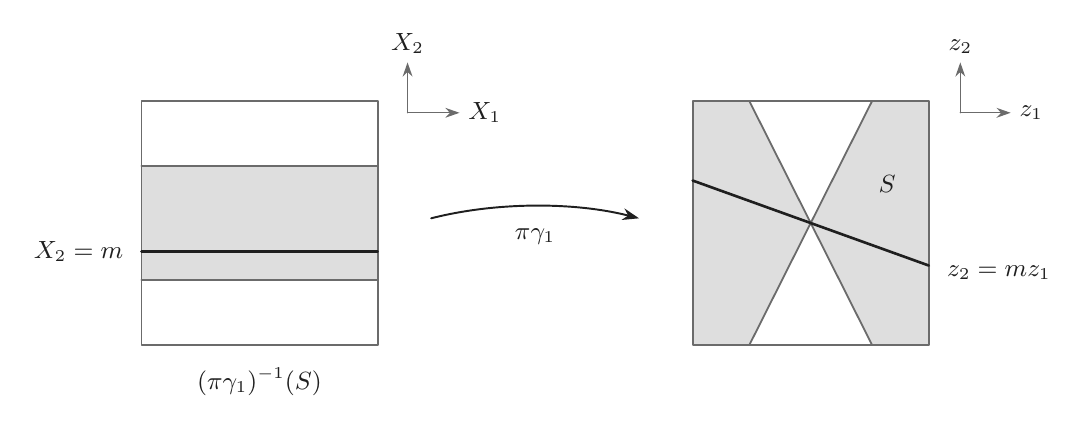
\begin{tikzpicture}[field/diagram]
    % Affine chart on the blow-up.
    \fill[FieldRegion] (-5,-0.72) rectangle (-2,0.72);
    \draw[field/secondary] (-5,-1.55) rectangle (-2,1.55);
    \draw[field/secondary] (-5,-0.72) -- (-2,-0.72)
                           (-5,0.72) -- (-2,0.72);
    \draw[field/curve] (-5,-0.36) -- (-2,-0.36);
    \node[anchor=east] at (-5.12,-0.36) {$X_2=m$};
    \node[below] at (-3.5,-1.73) {$(\pi\gamma_1)^{-1}(S)$};
    \draw[field/axis] (-1.62,1.40) -- (-0.96,1.40) node[right] {$X_1$};
    \draw[field/axis] (-1.62,1.40) -- (-1.62,2.04) node[above] {$X_2$};

    \draw[field/map] (-1.32,0.06)
        .. controls (-0.5,0.27) and (0.5,0.27) .. (1.32,0.06)
        node[midway, below=5pt] {$\pi\gamma_1$};

    % The two gray sectors are the cone S in the original coordinates.
    \fill[FieldRegion]
        (2,-1.55) -- (2.72,-1.55) -- (3.5,0)
        -- (2.72,1.55) -- (2,1.55) -- cycle;
    \fill[FieldRegion]
        (5,-1.55) -- (4.28,-1.55) -- (3.5,0)
        -- (4.28,1.55) -- (5,1.55) -- cycle;
    \draw[field/secondary] (2,-1.55) rectangle (5,1.55);
    \draw[field/secondary] (2.72,-1.55) -- (4.28,1.55)
                           (2.72,1.55) -- (4.28,-1.55);
    \draw[field/curve] (2,0.54) -- (5,-0.54);
    \node[anchor=west] at (5.12,-0.63) {$z_2=mz_1$};
    \node at (4.47,0.50) {$S$};
    \draw[field/axis] (5.40,1.40) -- (6.04,1.40) node[right] {$z_1$};
    \draw[field/axis] (5.40,1.40) -- (5.40,2.04) node[above] {$z_2$};
\end{tikzpicture}

        \FieldCaption{I}{9}{}
    \end{minipage}
\end{center}

In the figure, the line $z_2=mz_1$ in the $(z_1,z_2)$-plane corresponds to the affine line $X_2=m$ in the $(X_1,X_2)$-plane.

The construction we have described above works equally well if instead of $\mathbb C^n$ we take an open neighbourhood $U$ of $0\in\mathbb C^n$ and define $\Sigma_U\subset U\times P^{n-1}(\mathbb C)$ to be the intersection of $\Sigma$ with $U\times P^{n-1}(\mathbb C)$. We refer to $\Sigma_U$ as $U$ blown up at zero. The projection again restricts to a holomorphic map $\pi:\Sigma_U\longrightarrow U$ which induces a biholomorphic map between $\Sigma_U\setminus E$ and $U\setminus\{0\}$.

We now wish to generalise the construction above so that we can blow up arbitrary complex manifolds at a point. First, a lemma.

\FieldHeading{Lemma}{4.7.1}{}\FieldTarget{lemma:4.7.1}{4.7.1} Let $M$ and $\Sigma$ be complex manifolds with closed submanifolds $N$ and $X$ respectively. Suppose that for some open neighbourhood $U$ of $N$ in $M$ there exists a biholomorphism $\phi:U\setminus N\longrightarrow\Sigma\setminus X$. Then if we define
\[
M^*=(M\setminus N)\cup\Sigma,
\]
% Original book page 179
where we identify $x\in M\setminus N$ with $y\in\Sigma\setminus X$ if $\phi(x)=y$, $M^*$ has the natural structure of a complex manifold such that $M^*\setminus X$ is biholomorphic to $M\setminus N$. Furthermore, if $\phi$ is the restriction of a holomorphic map $\pi:U\longrightarrow\Sigma$, then $\pi$ induces a holomorphic map $\pi:M^*\longrightarrow M$ such that $\pi$ maps $M^*\setminus X$ biholomorphically onto $M\setminus N$.
\begin{proof}
The proof is quite elementary and we leave it to the reader.
\end{proof}

Suppose $M$ is a complex manifold of dimension $n$, $n>1$, and let $p\in M$. Choose a coordinate chart $(V,\phi)$ for $M$ such that $p\in V$ and $\phi(p)=0$. Set $U=\phi(V)$. Let $\Sigma$ denote the blow up of $U$ at 0 ($\Sigma_U$ in the notation above). Then $\phi^{-1}\pi:\Sigma\setminus E\longrightarrow V\setminus\{p\}$ is a biholomorphism and so we may apply Lemma~\ref{lemma:4.7.1} to construct the complex manifold
\[
B_p(M)=(M\setminus\{p\})\cup\Sigma
\]
together with the holomorphic map $\pi:B_p(M)\longrightarrow M$. We say that $B_p(M)$ is $M$ blown up at the point $p$ (or any of the other descriptions we gave previously for blowing up\IndexMark{idx-051}{blowing up@Blowing-up!with non singular centre@with non-singular centre} $\mathbb C^n$). We call $p$ the centre of the blowing up and $E=\pi^{-1}(p)$ the exceptional variety. Clearly $E$ is biholomorphic to $P^{n-1}(\mathbb C)$. The projection map $\pi:B_p(M)\longrightarrow M$ is a proper holomorphic map and restricts to a biholomorphism of $B_p(M)\setminus E$ with $M\setminus\{p\}$.

We may generalise the above construction to include centres which are closed complex submanifolds of $M$. First we describe the local situation. Regard $\mathbb C^m$ as the subspace $\mathbb C^m\times\{0\}$ of $\mathbb C^{m+n}$. We define $\mathbb C^{m+n}$ blown up along $\mathbb C^m$ to be the space $\mathbb C^m\times\Sigma$, where $\Sigma$ is $\mathbb C^n$ blown up at zero. In other words, we just blow up normal to $\mathbb C^m$ in $\mathbb C^{m+n}$. More generally, if $X$ is a closed submanifold of $M$ we may blow up $M$ along $X$ to construct a complex manifold $B_X(M)$ together with a holomorphic projection $\pi:B_X(M)\longrightarrow M$ which restricts to a biholomorphic map of $B_X(M)\setminus\pi^{-1}(X)$ onto $M\setminus X$. In this case the exceptional variety $\pi^{-1}(X)$ is a bundle over $X$ with fibre biholomorphic to $P^q(\mathbb C)$, where $q=\dim(M)-\dim(X)-1$. We give an example of this process below.

We shall now give some examples to show how blowing up may be used to ``desingularize\IndexMark{idx-171}{desingularization@Desingularization}'' analytic sets. Suppose that $X$ is an analytic subset of
% Original book page 180
the complex manifold $M$. Let $Y$ be a closed complex submanifold of $M$ which is a subset of $\operatorname{Sing}(X)$. Let us blow up $M$ along $Y$ to give the new complex manifold $B_Y(M)$. The set $\pi^{-1}(X)$ is an analytic subset of $B_Y(M)$. Necessarily $\pi^{-1}(X)$ contains the exceptional variety $E=\pi^{-1}(Y)$ and we define the \emph{strict transform}\IndexMark{idx-585}{strict transform@Strict transform} of $X$ to be the analytic subset $X^*=\overline{\pi^{-1}(X)\setminus E}$ of $B_Y(M)$. As our examples will show a careful choice of $Y$ will often result in $X^*$ having ``simpler'' singularities than $X$.

\paragraph*{Examples.}
\paragraph*{1.} Let $Z\subset\mathbb C^2$ denote the curve defined by $P(z_1,z_2)=(z_1-z_2)(z_1+z_2)=0$. $Z$ has an isolated singularity at zero. As above we let $\Sigma$ denote $\mathbb C^2$ blown up at zero and $\pi:\Sigma\longrightarrow\mathbb C^2$ the projection map. Set $\widetilde Z=\pi^{-1}(Z)$ and let $Z^*$ denote the strict transform of $Z$. To describe $\widetilde Z$ we use the atlas $\{(U_i,\phi_i):i=1,2\}$ that we previously constructed on $\Sigma$. For $i=1,2$, set $\widetilde Z_i=\phi_i(\widetilde Z\cap U_i)\subset\mathbb C^2$. Then $\widetilde Z_1$ is the zero set of $P(X_1,X_1X_2)$ and $\widetilde Z_2$ is the zero set of $P(X_1X_2,X_2)$. We have
\[
P(X_1,X_1X_2)=(X_1-X_1X_2)(X_1+X_1X_2)=X_1^2(1-X_2)(1+X_2).
\]
Now $X_1=0$ is just the equation of the exceptional variety (intersected with $U_1$) and so the strict transform $Z^*$ of $Z$ is the pair of distinct lines $X_2=\pm1$ (again intersected with $U_1$). A similar description holds in the chart $(U_2,\phi_2)$. Hence $Z^*$ consists of two distinct lines and, in particular, is non-singular.

\begin{center}
    \begin{minipage}{\linewidth}
        \centering
        % Figure 10. Curve diagrams deliberately have no area fill.
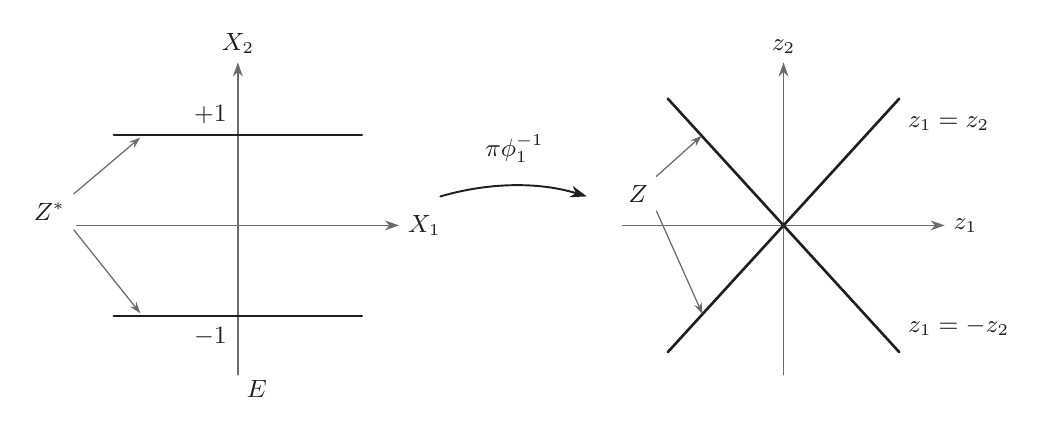
\begin{tikzpicture}[field/diagram, x=1.05cm, y=1.15cm]
    \draw[field/axis] (-1.95,0) -- (1.95,0) node[right] {$X_1$};
    \draw[field/axis] (0,-1.65) -- (0,1.8) node[above] {$X_2$};
    \draw[field/curve] (-1.50,1) -- (1.50,1)
                       (-1.50,-1) -- (1.50,-1);
    \node[above left, inner sep=3pt] at (0,1) {$+1$};
    \node[below left, inner sep=3pt] at (0,-1) {$-1$};
    \node[below right] at (0,-1.62) {$E$};
    \node (Zstar) at (-2.28,0.15) {$Z^*$};
    \draw[field/leader] (Zstar.north east) -- (-1.18,0.97);
    \draw[field/leader] (Zstar.south east) -- (-1.18,-0.97);
    \draw[field/map] (2.45,0.32)
        .. controls (3.05,0.48) and (3.65,0.48) .. (4.22,0.32)
        node[midway, above=5pt] {$\pi\phi_1^{-1}$};
    \begin{scope}[shift={(6.6,0)}]
        \draw[field/axis] (-1.95,0) -- (1.95,0) node[right] {$z_1$};
        \draw[field/axis] (0,-1.65) -- (0,1.8) node[above] {$z_2$};
        \draw[field/curve] (-1.4,-1.4) -- (1.4,1.4)
                           (-1.4,1.4) -- (1.4,-1.4);
        \node[anchor=west] at (1.40,1.12) {$z_1=z_2$};
        \node[anchor=west] at (1.40,-1.12) {$z_1=-z_2$};
        \node (Z) at (-1.76,0.35) {$Z$};
        \draw[field/leader] (Z.north east) -- (-0.99,0.99);
        \draw[field/leader] (Z.south east) -- (-0.98,-0.98);
    \end{scope}
\end{tikzpicture}

        \FieldCaption{I}{10}{}
    \end{minipage}
\end{center}
% Original book page 181
\paragraph*{2.} Let $Z\subset\mathbb C^2$ be the curve defined by $P(z_1,z_2)=z_1^2-z_2^3=0$. $Z$ has an isolated singularity at zero. Repeating the argument above, we see that $\widetilde Z_1\subset\mathbb C^2$ is the zero locus of $X_1^2-X_1^3X_2^3=X_1^2(1-X_1X_2^3)$. That is, the intersection of $Z^*$ with $U_1$ is the non-singular curve $1=X_1X_2^3$ (notice that this curve does not meet the exceptional variety $X_1=0$---in $U_1$). Similarly, $\widetilde Z_2$ is the zero locus of $X_1^2X_2^2-X_2^3=X_2^2(X_1^2-X_2)$. Now $X_2=0$ is the equation of the exceptional variety in $U_2$ and so the intersection of $Z^*$ with $U_2$ is the parabola $X_2=X_1^2$, which is of course non-singular. Hence $Z^*$ is non-singular.

\begin{center}
    \begin{minipage}{\linewidth}
        \centering
        % Figure 11. Smooth parametric plots preserve the indicated equations.
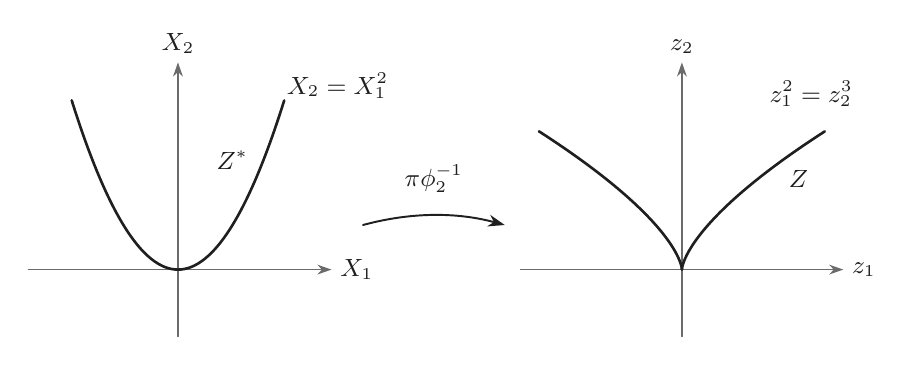
\begin{tikzpicture}[field/diagram, x=1.0cm, y=1.18cm]
    \draw[field/axis] (-1.9,0) -- (1.95,0) node[right] {$X_1$};
    \draw[field/axis] (0,-0.72) -- (0,2.23) node[above] {$X_2$};
    \draw[field/curve, domain=-1.35:1.35, samples=65, smooth]
        plot (\x,{\x*\x});
    \node[anchor=west] at (1.27,1.98) {$X_2=X_1^2$};
    \node at (0.69,1.18) {$Z^*$};
    \draw[field/map] (2.35,0.48)
        .. controls (2.96,0.62) and (3.54,0.62) .. (4.15,0.48)
        node[midway, above=5pt] {$\pi\phi_2^{-1}$};
    \begin{scope}[shift={(6.4,0)}]
        \draw[field/axis] (-2.05,0) -- (2.05,0) node[right] {$z_1$};
        \draw[field/axis] (0,-0.72) -- (0,2.23) node[above] {$z_2$};
        % The branches meet with their common vertical tangent at the cusp.
        \draw[field/curve, domain=-1.22:0, samples=65, smooth, variable=\t]
            plot ({\t*\t*\t},{\t*\t});
        \draw[field/curve, domain=0:1.22, samples=65, smooth, variable=\t]
            plot ({\t*\t*\t},{\t*\t});
        \node[anchor=west] at (1.0,1.89) {$z_1^2=z_2^3$};
        \node at (1.48,0.97) {$Z$};
    \end{scope}
\end{tikzpicture}

        \FieldCaption{I}{11}{}
    \end{minipage}
\end{center}

If instead we had started with the curve $z_1^2=z_2^5$, we would find that $Z^*\cap U_2$ was the curve $X_1^2=X_2^3$. Hence a further blowing up, this time of the manifold $\Sigma$, would remove the singularity. Without too much difficulty this technique will effectively resolve the singularities\IndexMark{idx-172}{desingularization@Desingularization} of all curves. Details may be found in Walker \cite{bib:I:walker-r:1}, Mumford \cite{bib:I:mumford-d:1} or Hartshorne \cite{bib:I:hartshorne-r:2}.

Fundamental results of Hironaka \cite{bib:I:hironaka-h:1,bib:I:hironaka-h:2}, following on work of Walker and Zariski assert that we can always resolve singularities of complex analytic sets. Specifically, if $X$ is a complex analytic subset of a complex manifold $M$, there exists a (locally finite) sequence
\[
M_\Lambda\xrightarrow{\pi_\Lambda}M_{\Lambda-1}\xrightarrow{\pi_{\Lambda-1}}\cdots\longrightarrow M_1\xrightarrow{\pi_1}M
\]
% Original book page 182
of blowing ups of $M$, with non-singular centres, such that the iterated strict transform of $X$ is a non-singular submanifold of $M_\Lambda$. The proof of this result is extremely hard. Much of the difficulty lies with choosing the centres so that when we blow up along them the singularities are somehow simplified. A proof of the desingularization theorem, together with many helpful examples is given in Hironaka \cite{bib:I:hironaka-h:2}.

The next example shows that one cannot hope to give simple proofs of the desingularization theorem by working with a restricted class of analytic sets such as hypersurfaces with isolated singularities.

\paragraph*{Example 3.} Let $Z\subset\mathbb C^3$ be the hypersurface defined by $z_1^5=z_2z_3^6-z_2^6z_3$. $Z$ has an isolated singularity at 0. Blow up $\mathbb C^3$ at zero. We now describe $\widetilde Z_i=\widetilde Z\cap U_i$, $1\leq i\leq3$.

$\widetilde Z_1$ is the zero locus of $X_1^5(1-X_1^2X_2X_3^6+X_1^2X_2^6X_3)$ and so the strict transform $Z^*$ intersects $U_1$ in the non-singular hypersurface $1=X_1^2X_2X_3^6-X_1^2X_2^6X_3$.

$\widetilde Z_2$ is the zero locus of $X_2^5(X_1^5-X_2^2X_3^6-X_2^2X_3)$. Therefore $Z^*\cap U_2$ is the hypersurface $X_1^5=X_2^2X_3^6-X_2^2X_3$. Now $\operatorname{Sing}(Z^*\cap U_2)$ is the set $X_1=X_2=0$. In particular, $Z^*\cap U_2$ no longer has an isolated singularity.

Just as for $\widetilde Z_2$, we find that $Z^*\cap U_3$ is the curve $X_1^5=X_3^2X_2-X_3^2X_2^6$ with singular locus $X_1=X_3=0$.

It follows from the above that $\operatorname{Sing}(Z^*)$ is a subset of the exceptional variety $P^2(\mathbb C)$ and is in fact the hyperplane $X_1=0$ (Here we take homogeneous coordinates $(X_1,X_2,X_3)$ on $P^2(\mathbb C)$). In other words $\operatorname{Sing}(Z^*)$ is biholomorphic to the Riemann sphere $P^1(\mathbb C)$.

We now blow up $\Sigma$ along $\operatorname{Sing}(Z^*)$. Let us work in $U_2$. $Z^*\cap U_2$ is the hypersurface $X_1^5=X_2^2X_3^6-X_2^2X_3$ with singular set $X_1=X_2=0$. Blowing up along the $X_3$-axis, we make the transformations $X_1=Y_1Y_2$, $X_2=Y_2$, $X_3=Y_3$ to obtain the hypersurface
\[
Y_1^5Y_2^5-Y_2^2Y_3^6+Y_2^2Y_3=Y_2^2(Y_1^5Y_2^3-Y_3^6+Y_3)=0.
\]
% Original book page 183
The strict transform is the hypersurface $Y_3=Y_3^6-Y_1^5Y_2^3$ which is of course non-singular. A similar result holds in $U_3$ and so the strict transform of $Z^*$ obtained by blowing up $\Sigma$ along $\operatorname{Sing}(Z^*)$ is a non-singular hypersurface.

We now wish to say a few words about the \emph{embedded resolution of singularities}\IndexMark{idx-224}{embedded resolution of singularities@Embedded resolution of singularities}\IndexMark{idx-514}{resolution of singularities@Resolution of singularities}. First we give a definition: Suppose that $Y$ is an analytic hypersurface in the complex manifold $N$. For each $x\in Y$, we may write $I_x(Y)=(p_1,\ldots,p_k)$, where $p_1,\ldots,p_k$ are the local defining equations for the irreducible components of $Y$ passing through $x$. We say that $Y$ is a \emph{hypersurface with} (or \emph{in}) \emph{normal crossings}\IndexMark{idx-190}{divisor in normal crossings@Divisor in normal crossings}\IndexMark{idx-322}{hypersurface@Hypersurface!in normal crossings@in normal crossings}\IndexMark{idx-407}{normal crossings@Normal crossings} if (1) Each irreducible component of $Y$ is non-singular; (2) For each $x\in Y$, $\{dp_1(x),\ldots,dp_k(x)\}$ form a linearly independent set.

Notice that the second condition implies that not more than $\operatorname{dimension}(N)$ irreducible components of $Y$ pass through any point of $N$. Condition (2) may also be given in terms of the tangent spaces to the irreducible components of $Y$ at $x$. We require $\dim(T_xN\cap\bigcap T_xY_j)=n-k$, where we assume that there are $k$ irreducible components $Y_j$ of $Y$ passing through $x$. Yet another equivalent formulation is that given $x\in Y$, we can choose complex analytic coordinates $(z_1,\ldots,z_n)$ at $x$ such that $Y$ is locally the zero set of the function $u(z)z_1^{m_1}\cdots z_k^{m_k}$, $u(0)\neq0$.

\begin{center}
    \begin{minipage}{\linewidth}
        \centering
        % Figure 12. Pairwise crossings versus a triple point.
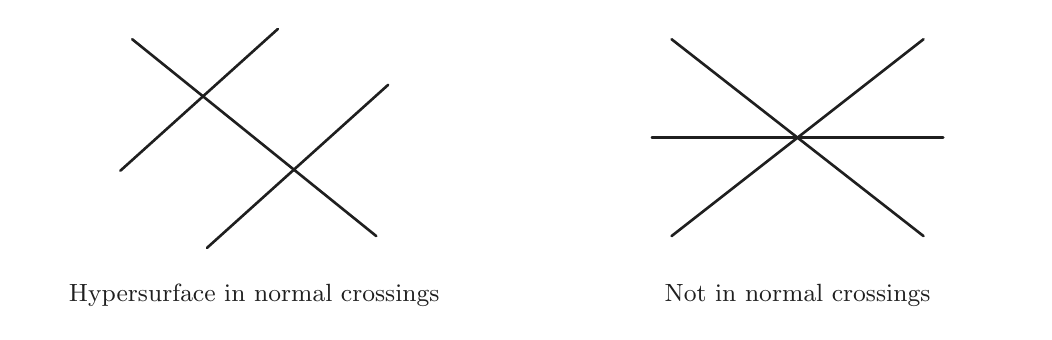
\begin{tikzpicture}[field/diagram]
    \begin{scope}[shift={(-3.45,0)}]
        \draw[field/curve] (-1.55,1.25) -- (1.55,-1.25);
        \draw[field/curve] (-1.7,-0.42) -- (0.30,1.38);
        \draw[field/curve] (-0.60,-1.4) -- (1.70,0.67);
        \node[align=center, text width=5.6cm] at (0,-2.00)
            {Hypersurface in normal crossings};
    \end{scope}
    \begin{scope}[shift={(3.45,0)}]
        \draw[field/curve] (-1.6,-1.25) -- (1.6,1.25);
        \draw[field/curve] (-1.6,1.25) -- (1.6,-1.25);
        \draw[field/curve] (-1.85,0) -- (1.85,0);
        \node[align=center, text width=5.6cm] at (0,-2.00)
            {Not in normal crossings};
    \end{scope}
\end{tikzpicture}

        \FieldCaption{I}{12}{}
    \end{minipage}
\end{center}
% Original book page 184
Suppose $d\in\mathcal D(N)$. We say that $d$ is a \emph{divisor in normal crossings} if the hypersurface $|d|$ is in normal crossings. If $d$ is in normal crossings and $x\in|d|$, we may choose complex analytic coordinates at $x$ so that $d$ is locally given as the divisor of the meromorphic function $u(z)z_1^{m_1}\cdots z_k^{m_k}$, $u(0)\neq0$.

Now suppose $X$ is an analytic subset of the complex manifold $M$. The embedded resolution of singularities\IndexMark{idx-225}{embedded resolution of singularities@Embedded resolution of singularities} theorem asserts that we can find a proper map $\pi:\widetilde M\longrightarrow M$ of complex manifolds which is a (locally finite) composition of blowing ups with non-singular centres such that $\widetilde X=\pi^{-1}(X)$ is non-singular and $\pi^{-1}(\operatorname{Sing}(X))$ is a divisor in $\widetilde X$ in normal crossings. A proof may be found in Hironaka \cite{bib:I:hironaka-h:2}.

\paragraph*{Examples.}
\paragraph*{4.} The resolution of the curve $(z_1-z_2)(z_1+z_2)=0$ given in example 1 above is an embedded resolution.

\paragraph*{5.} The resolution of the curve $z_1^2-z_2^3=0$ given in example 2 above is not an embedded resolution. Two further blowing ups are needed to obtain an embedded resolution:

\begin{center}
    \begin{minipage}{\linewidth}
        \centering
        % Figure 13. Blow-down arrows still point from right to left.
% Dark curves denote Z^*; secondary gray curves denote exceptional divisors.
\begin{tikzpicture}[field/diagram, x=1.05cm, y=1.05cm]
    \draw[field/secondary] (-1.48,0) -- (1.48,0)
        node[right] {$E_1$};
    \draw[field/curve, domain=-1.35:1.35, samples=55, smooth]
        plot (\x,{0.75*\x*\x});
    \node at (0.62,1.20) {$Z^*$};
    \draw[field/map] (2.75,0.53)
        .. controls (2.40,0.65) and (2.14,0.65) .. (1.84,0.53)
        node[midway, below=4pt] {$\pi$};

    \begin{scope}[shift={(4.40,0)}]
        \draw[field/secondary] (-1.20,0) -- (1.20,0)
            node[right] {$E_1$};
        \draw[field/secondary] (0,-0.94) -- (0,2.46)
            node[above] {$E_2$};
        \draw[field/curve] (-0.68,-0.91) -- (1.08,1.44);
        \node[anchor=west] at (1.17,1.48) {$Z^*$};
    \end{scope}
    \draw[field/map] (7.08,0.53)
        .. controls (6.75,0.65) and (6.40,0.65) .. (6.07,0.53)
        node[midway, below=4pt] {$\pi$};

    \begin{scope}[shift={(8.80,0)}]
        \draw[field/secondary] (-1.18,2) -- (1.18,2) node[right] {$E_1$};
        \draw[field/secondary] (-1.18,1) -- (1.18,1) node[right] {$E_2$};
        \draw[field/secondary] (0,-0.94) -- (0,2.48);
        \draw[field/curve] (-1.18,0) -- (1.18,0) node[right] {$Z^*$};
        \node[below] at (0,-0.94) {$E_3$};
    \end{scope}
\end{tikzpicture}

        \FieldCaption{I}{13}{}
    \end{minipage}
\end{center}
% Original book page 185
We conclude this chapter with some remarks on the role of blowing up in the classification theory of compact complex manifolds, especially complex surfaces.

First notice that we can use blowing up to define a relation between complex manifolds of the same dimension. Thus we shall say that $M$ is B-related to $N$ if $M$ may be obtained by blowing up $N$ a finite number of times. If $M$ and $N$ are complex surfaces then the centres of the blowing ups must always be points and the exceptional varieties are always biholomorphic to $P^1(\mathbb C)$. Now suppose that $E$ is a complex submanifold of the complex surface $M$ which is biholomorphic to $P^1(\mathbb C)$. It follows from a theorem of Grauert \cite{bib:I:grauert-h:1}, that if the self-intersection number of $E$ is $-1$ (``$E^2=-1$'') then we can \emph{blow down} $E$ to a point. That is, there exists a complex surface $N$ such that for some $p\in N$, $B_p(N)=M$ and the exceptional variety of the blowing up is $E$. We call such a variety $E$ an \emph{exceptional curve of first kind}\IndexMark{idx-241}{exceptional curve of first kind@Exceptional curve of first kind}. We can now define an equivalence relation between compact complex surfaces. We say that the surfaces $M$ and $N$ are B-equivalent if $M$ can be obtained from $N$ by a finite number of blowing ups and blowing downs. We say that a complex surface is a \emph{relatively minimal model}\IndexMark{idx-396}{minimal model@Minimal model} if and only if it does not contain any exceptional curves of the first kind. Every compact complex surface can be obtained from a relatively minimal model by a finite succession of blowing ups.

In Kodaira \cite{bib:I:kodaira-k:2} there is a description of the relatively minimal models of compact complex surfaces as well as a description of the classification of compact complex surfaces. A useful survey of Kodaira's work, together with further references, may be found in Sundararaman \cite{bib:I:sundararaman-d:1}. See also Ueno \cite{bib:I:ueno-k:1}.

It is an important problem to find properties of complex manifolds invariant under blowing up or blowing down\IndexMark{idx-052}{blowing down@Blowing down} (in algebraic geometry the corresponding problem is that of finding birational invariants\IndexMark{idx-049}{birational invariant@Birational invariant}). We shall describe one invariant here (see also \hyperref[sec:5:9]{\S9, Chapter 5}) and refer the reader to the references cited above for the description of other invariants and proofs. Let $M$ be a compact complex manifold with field of meromorphic functions $\mathcal M(M)$. We let $t(M)$ denote the transcendence degree of $\mathcal M(M)$ over $\mathbb C$. A result of Thimm \cite{bib:I:thimm-w:1} (see also Remmert \cite{bib:I:remmert-r:1}, Siegel \cite{bib:I:siegel-c-l:2}) asserts that
% Original book page 186
$t(M)\leq\operatorname{dimension}(M)$. If $M$ is algebraic, $t(M)=\operatorname{dimension}(M)$. We have the important result that $t(M)$ is invariant under blowing ups. Thus surfaces with different transcendence degrees cannot have the same relatively minimal models. If $t(M)=\operatorname{dimension}(M)$ we say that $M$ is a \emph{Moishezon manifold}\IndexMark{idx-399}{moishezon manifold@Moishezon manifold}. If $\operatorname{dimension}(M)=2$, every Moishezon manifold is algebraic by a theorem of Kodaira \cite{bib:I:kodaira-k:2}. The theory of Moishezon manifolds is expounded in Moishezon \cite{bib:I:moishezon-b-g:1}. We remark that even though a Moishezon manifold $M$ need not be algebraic (at least if $\operatorname{dimension}(M)>2$), there exists a finite sequence of blowing ups of $M$ such that the resulting manifold is algebraic (For a proof see Moishezon \cite[Chapter 2]{bib:I:moishezon-b-g:1}). Of course, if $M$ is algebraic, then any finite sequence of blowing ups of $M$ with non-singular centres (necessarily algebraic) will give an algebraic manifold.

\subsection*{Exercises}
\begin{enumerate}
\item Blow up the surface $zx^2=y^2$ at zero. Observe that blowing up at the (geometrically) most singular points does not always work. Now find a desingularization of the surface.
\item Verify that the surface $x^2y^2-z^6+x^6+y^6=0$ has an isolated singularity at zero. Show that when we blow up at zero, the new surface has a singular set with singularities.
\end{enumerate}

\part{Calculus, Sheaf Theory and Coherent Sheaves}
% Source: Part II, original PDF page 4 (title page).
% Preserve continuous combined pagination and the original Part II TeX layout.
\clearpage
\begingroup
    \thispagestyle{empty}
    \noindent London Mathematical Society Lecture Note Series.\quad 66
    \vfill
    {\Huge\bfseries\raggedright Several Complex Variables and Complex Manifolds II\par}
    \vspace{2cm}
    {\Large MIKE FIELD\par}
    Senior Lecturer, Department of Pure Mathematics,\par
    University of Sydney
    \vfill
    CAMBRIDGE UNIVERSITY PRESS\par\medskip
    CAMBRIDGE\par\medskip
    LONDON\quad NEW YORK\quad NEW ROCHELLE\par\medskip
    MELBOURNE\quad SYDNEY
    \clearpage
\endgroup

% Publication data for Part II, placed directly after its title page.
% No printed heading or table-of-contents entry; pagination remains continuous.
\clearpage
\begingroup
    \thispagestyle{empty}
    \markboth{}{}
\noindent London Mathematical Society Lecture Note Series 66.\par
\emph{Several Complex Variables and Complex Manifolds II}. Mike Field.\par
Senior Lecturer, Department of Pure Mathematics, University of Sydney.\par
Cambridge University Press. Cambridge; London; New York; New Rochelle; Melbourne; Sydney.

\noindent Published by the Press Syndicate of the University of Cambridge.\par
The Pitt Building, Trumpington Street, Cambridge CB2 1RP.\par
32 East 57th Street, New York, NY 10022, USA.\par
296 Beaconsfield Parade, Middle Park, Melbourne 3206, Australia.

\noindent\textcopyright\ Cambridge University Press 1982. First published in 1982.\par
Library of Congress catalogue card number 81-21590.

\noindent British Library cataloguing in publication data:\par
Field, Mike. Several complex variables and complex manifolds 2.---(London Mathematical Society Lecture Note Series 65, ISSN 0076-0552.)\par
1. Topological spaces. 2. Manifolds (Mathematics). I. Title. II. Series.\par
514'.223\qquad QA611.A1\par
ISBN 0 521 28888 6. Transferred to digital printing 1999.

\medskip
\noindent{\small The series number 65 in the Part II cataloguing record is reproduced from its copyright page; its cover and title page state 66. The shared publisher's series catalogue and the Part II back-cover text are retained at the end of this transcription.}
    \clearpage
\endgroup

\chapter{Calculus on Complex Manifolds}\label{ch:5}
\ChapterFiveIntroduction
% Source PDF page 10; printed page 1
\section{Review of linear algebra}\label{sec:5:1}
In this section we shall review some elementary linear algebra that does not depend on the assumption of an inner product structure. We shall generally omit proofs (usually simple) referring the reader to any one of the many texts in linear algebra. All vector spaces in this section will be assumed real and finite dimensional.

\begin{originaltheorem}{Definition}{5.1.1}\FieldTarget{definition:5.1.1}{5.1.1}
A \emph{graded vector space}\IndexMark{idx-270}{graded vector space@Graded vector space} $\mathbf E$ is a collection $\{E_0,E_1,\ldots\}$ of vector spaces indexed by the positive integers. We write $\mathbf E=\{E_0,E_1,\ldots\}$ and set $\mathbf E_n=E_n$. We call $E_n$ the $n$th. component of $\mathbf E$. A \emph{morphism} $\mathbf T:\mathbf E\longrightarrow\mathbf F$, of degree $r\geq0$, of graded vector spaces is a collection of linear maps $T_i:E_i\to F_{i+r}$ indexed by the positive integers.
\end{originaltheorem}
% Source PDF page 11; printed page 2
\paragraph{Examples.}
\begin{enumerate}
\item Associated to the vector space $E$ we may define the graded vector spaces $\boldsymbol\otimes E$, $\boldsymbol\Lambda E$ and $\boldsymbol\odot E$ whose $n$th. components are respectively $\otimes^n E$, $\Lambda^n E$ and $\odot^n E$ ($n$th. tensor, exterior and symmetric powers of $E$ respectively).
\item A linear map $T:E\to F$ induces degree zero morphisms $\boldsymbol\otimes T:\boldsymbol\otimes E\longrightarrow\boldsymbol\otimes F$, $\boldsymbol\Lambda T:\boldsymbol\Lambda E\longrightarrow\boldsymbol\Lambda F$, $\boldsymbol\odot T:\boldsymbol\odot E\longrightarrow\boldsymbol\odot F$ whose $n$th. components are $\otimes^n T$, $\Lambda^n T$ and $\odot^n T$ respectively.
\end{enumerate}
\begin{originaltheorem}{Definition}{5.1.2}\FieldTarget{definition:5.1.2}{5.1.2}
Let $\mathbf E$ and $\mathbf F$ be graded vector spaces. Then
\begin{enumerate}
\item The \emph{direct sum} of $\mathbf E$ and $\mathbf F$ is the graded vector space $\mathbf E\boldsymbol\oplus\mathbf F$ whose $n$th. component is $E_n\oplus F_n$.
\item The \emph{tensor product} of $\mathbf E$ and $\mathbf F$ is the graded vector space $\mathbf E\boldsymbol\otimes\mathbf F$ whose $n$th. component is $\displaystyle\bigoplus_{r+s=n}E_r\otimes F_s$.
\end{enumerate}
\end{originaltheorem}
\begin{originaltheorem}{Definition}{5.1.3}\FieldTarget{definition:5.1.3}{5.1.3}
A \emph{graded vector space algebra}\IndexMark{idx-271}{graded vector space@Graded vector space!algebra@algebra} consists of a graded vector space $\mathbf E$ together with a morphism of degree zero $\phi:\mathbf E\boldsymbol\otimes\mathbf E\longrightarrow\mathbf E$, written $\phi(A\otimes B)=AB$, satisfying the following properties
\begin{enumerate}
\item The multiplication defined by $\phi$ is associative.
\item There exists a unit element in $\mathbf E$ for the multiplication.
\end{enumerate}
The algebra is said to be \emph{commutative} if $AB=(-1)^{pq}BA$, $A\in E_p$, $B\in E_q$.
\end{originaltheorem}
\paragraph{Remark.} The universal factorization property for the tensor product implies that we may equivalently suppose that $\phi$ is a bilinear map on $\mathbf E\times\mathbf E$.
\paragraph{Example 3.} Given a vector space $E$, $\boldsymbol\otimes E$, $\boldsymbol\Lambda E$ and $\boldsymbol\odot E$ are graded vector space algebras with respective algebra operations of tensor\IndexMark{idx-603}{tensor algebra of vector space@Tensor algebra of vector space} product, exterior\IndexMark{idx-248}{exterior algebra of vector space@Exterior algebra of vector space} or wedge product and symmetric\IndexMark{idx-596}{symmetric tensor algebra of vector space@Symmetric tensor algebra of vector space} product. $\boldsymbol\Lambda E$ is commutative\IndexMark{idx-099}{commutative vector space algebra@Commutative vector space algebra}.
\begin{originaltheorem}{Proposition}{5.1.4}\FieldTarget{proposition:5.1.4}{5.1.4}
Let $E$ and $F$ be vector spaces. Then $\boldsymbol\Lambda E\boldsymbol\otimes\boldsymbol\Lambda F$ has the natural structure of a commutative graded algebra with wedge product defined by
% Source PDF page 12; printed page 3
\[
(X\otimes Y)\wedge(X'\otimes Y')=(-1)^{pq}(X\wedge X')\otimes(Y\wedge Y'),
\]
where $X\in\boldsymbol\Lambda E$, $Y\in\Lambda^p F$, $X'\in\Lambda^q E$, $Y'\in\boldsymbol\Lambda F$.
\end{originaltheorem}
\begin{proof}
We remark only that in all results of this type it is enough to define the operation or map on a set of generators for the algebra.
\end{proof}
Before stating the next result we remark that we say a morphism of graded vector spaces is an \emph{isomorphism} if it is invertible and of degree zero. An isomorphism of graded vector space algebras will, in addition, preserve the algebra structures.
\begin{originaltheorem}{Theorem}{5.1.5}\FieldTarget{theorem:5.1.5}{5.1.5}
If $E$ and $F$ are vector spaces we have a canonical isomorphism of commutative graded algebras
\[
\boldsymbol\Lambda(E\oplus F)\approx\boldsymbol\Lambda E\boldsymbol\otimes\boldsymbol\Lambda F.
\]
In particular,
\[
\boldsymbol\Lambda(E\oplus F)_p\approx\bigoplus_{r+s=p}\Lambda^r E\otimes\Lambda^s F,\quad p\geq0.
\]
\end{originaltheorem}
\begin{proof}
For $r,s\geq0$ we define $\mu_{r,s}:\Lambda^r E\otimes\Lambda^s F\to\boldsymbol\Lambda(E\oplus F)_{r+s}$ by
\[
\begin{split}
\mu_{r,s}(e_1\wedge\cdots\wedge e_r\otimes f_1\wedge\cdots\wedge f_s)
={}&(e_1+0)\wedge\cdots\wedge(e_r+0)\\
&\wedge(f_1+0)\wedge\cdots\wedge(f_s+0),
\end{split}
\]
where $e_i\in E$, $1\leq i\leq r$, $f_j\in F$, $1\leq j\leq s$, and the wedge product on the right hand side of the above relation is taken in $\Lambda^{r+s}(E\oplus F)$. We leave it to the reader to verify that the maps $\mu_{r,s}$ define the required morphism.
\end{proof}
Given a vector space $E$ it is possible to identify $\boldsymbol\Lambda E$ and $\boldsymbol\odot E$ with graded subspaces (\emph{not} subalgebras) of $\boldsymbol\otimes E$ and we now indicate how to do this in the case of exterior powers of $E$. Fix a positive integer $p$ and let $S_p$ denote the symmetric group on $p$ symbols. We define a representation $T:S_p\to\operatorname{GL}(\otimes^p E)$ of $S_p$ by
\[
T(\sigma)(e_1\otimes\cdots\otimes e_p)=\operatorname{sign}(\sigma)e_{\sigma(1)}\otimes\cdots\otimes e_{\sigma(p)},
\]
where $e_j\in E$, $1\leq j\leq p$, $\sigma\in S_p$. Let $\operatorname{Alt}_p(E)$ denote the fixed point set of the corresponding action of $S_p$ on $\otimes^p E$. Elements of $\operatorname{Alt}_p(E)$
% Source PDF page 13; printed page 4
are called \emph{alternating tensors}\IndexMark{idx-006}{alternating tensor@Alternating tensor} of order $p$. The map $\wedge:\otimes^p E\to\Lambda^p E$ defined by mapping $e_1\otimes\cdots\otimes e_p$ to $e_1\wedge\cdots\wedge e_p$ induces a linear isomorphism of $\operatorname{Alt}_p(E)$ with $\Lambda^p E$. To see this observe that we have a projection map $\operatorname{Alt}:\otimes^p E\to\operatorname{Alt}_p(E)$ defined by
\[
\operatorname{Alt}(e_1\otimes\cdots\otimes e_p)=\frac1{p!}\sum_{\sigma\in S_p}T(\sigma)(e_1\otimes\cdots\otimes e_p).
\]
Clearly $\operatorname{Kernel}(\operatorname{Alt})=\operatorname{Kernel}(\wedge)$ and so $\operatorname{Alt}_p(E)\approx\Lambda^p E$.
\paragraph{Remark.} Under the identification of $\Lambda^p E$ with $\operatorname{Alt}_p(E)$ given by this isomorphism we see that
\[
e_1\wedge\cdots\wedge e_p=\frac1{p!}\sum_{\sigma\in S_p}\operatorname{sign}(\sigma)e_{\sigma(1)}\otimes\cdots\otimes e_{\sigma(p)}.
\]
Let $E'=L_{\mathbb R}(E,\mathbb R)$ denote the dual space of $E$ and $\langle\ ,\ \rangle:E\times E'\to\mathbb R$ denote the dual pairing\IndexMark{idx-213}{dual pairing@Dual pairing} between $E$ and $E'$. For $p\geq0$, we have dual pairings $\otimes^p E\times\otimes^p E'\to\mathbb R$, $\Lambda^p E\times\Lambda^p E'\to\mathbb R$ respectively defined by
\[
\langle e_1\otimes\cdots\otimes e_p,\phi_1\otimes\cdots\otimes\phi_p\rangle=\prod_{i=1}^p\langle e_i,\phi_i\rangle
\]
\[
\langle e_1\wedge\cdots\wedge e_p,\phi_1\wedge\cdots\wedge\phi_p\rangle=\det[\langle e_i,\phi_j\rangle],
\]
where $e_i\in E$, $\phi_i\in E'$, $1\leq i\leq p$. Using these pairings we identify the dual spaces of $\otimes^p E$, $\Lambda^p E$ with $\otimes^p E'$, $\Lambda^p E'$ respectively. Notice that the dual pairing of $\otimes^p E$ with $\otimes^p E'$ induces a pairing of $\operatorname{Alt}_p(E)$ with $\operatorname{Alt}_p(E')$ and so a pairing of $\Lambda^p E$ with $\Lambda^p E'$. This pairing differs from the pairing we have defined between $\Lambda^p E$ and $\Lambda^p E'$ by a factor $p!$

We leave the case of the dual pairing for the symmetric powers of $E$ as an exercise.

For $p>0$, we define the linear map $U:\Lambda^p E\to E\otimes\Lambda^{p-1}E$ by
\[
U(e_1\wedge\cdots\wedge e_p)=\sum_{j=1}^p(-1)^{j+1}e_j\otimes e_1\wedge\cdots\wedge\widehat e_j\wedge\cdots\wedge e_p,
\]
where $e_j\in E$, $1\leq j\leq p$, and ``$\widehat{\ }$'' as usual denotes omission.
% Source PDF page 14; printed page 5
\paragraph{Properties of the map $U$.}
\begin{enumerate}
\item The operator $U$ is the transpose of $\wedge$, that is,
\[
\langle UX,\phi\otimes\psi\rangle=\langle X,\phi\wedge\psi\rangle,
\]
for all $X\in\Lambda^p E$, $\phi\in E'$, $\psi\in\Lambda^{p-1}E'$.
\item If $X\in\Lambda^p E$, $\wedge U(X)=pX$.
\item If $Z\in E\otimes\Lambda^p E$, then $U(\wedge Z)=Z-\wedge^{13}(I\otimes U)(Z)$, where $\wedge^{13}$ denotes the operation of wedging the first factor of $E\otimes E\otimes\Lambda^{p-1}E$ into the third factor.
\item If we iterate $U$, the map $U^p:\Lambda^q E\to\otimes^p E\otimes\Lambda^{q-p}E$ satisfies the relation $\wedge U^p=q!/(q-p)!\ I$, where $\wedge:\otimes^p E\otimes\Lambda^{q-p}E\to\Lambda^q E$ is just the operation of wedge product. In particular, if we identify $\Lambda^p E$ with $\operatorname{Alt}_p(E)$, we see that $\operatorname{Alt}\,U^p=p!I$, $p\geq0$.
\end{enumerate}
Properties 1--3 are easily proved by working on generators, property 4 may be proved by induction on $p$.

We conclude this section by describing the operation of \emph{contraction}\IndexMark{idx-133}{contraction@Contraction} or \emph{interior product}\IndexMark{idx-329}{interior product@Interior product} of tensors. First observe that since the dual pairing $E'\times E\to\mathbb R$ is bilinear it corresponds to a linear map $E'\otimes E\to\mathbb R$. This map is usually referred to as ``trace\IndexMark{idx-613}{trace@Trace}'' as if we use the natural identification of $E'\otimes E$ with $L(E,E)$ it corresponds to the operation of taking the trace of a linear map. Trace is the simplest example of a contraction operation and we shall now consider generalisations. With a view to later applications we work with tensor products of \emph{exterior} powers of vector spaces. Actually this is no loss of generality since $\Lambda^1 E=E$, $\Lambda^1 E'=E'$.

Suppose $p\geq q\geq0$. We define the linear map
\[
\mathsf C:\Lambda^p E\otimes\Lambda^q E'\longrightarrow\Lambda^{p-q}E
\]
by requiring that
\[
\langle\mathsf C(X\otimes\phi),\psi\rangle=\langle\phi\wedge\psi,X\rangle
\]
% Source PDF page 15; printed page 6
for all $X\in\Lambda^p E$, $\psi\in\Lambda^{p-q}E'$, $\phi\in\Lambda^q E'$. We similarly define
\[
\mathsf C:\Lambda^p E\otimes\Lambda^q E'\to\Lambda^{q-p}E'
\]
in case $q\geq p$.

Given $X\in\Lambda^p E$ and $q\geq p$ we define
\[
\mathsf C_X:\Lambda^q E'\to\Lambda^{q-p}E'
\]
by $\mathsf C_X(\phi)=\mathsf C(X\otimes\phi)$, $\phi\in\Lambda^q E'$. We similarly define $\mathsf C_\phi$ for $\phi\in\Lambda^p E'$. We call $\mathsf C$ a \emph{contraction} (operator) and $\mathsf C_X$ \emph{contraction with $X$}.

\paragraph{Properties of the contraction operators $\mathsf C$, $\mathsf C_X$, $\mathsf C_\phi$.}
\begin{enumerate}
\item For $p\geq0$, the map $\mathsf C:\Lambda^p E\otimes\Lambda^p E'\to\mathbb R$ is equal to the dual pairing of $\Lambda^p E$ with $\Lambda^p E'$.
\item $\mathsf C_X$ is the transpose of the operator ``wedge product with $X$''. That is,
\[
\langle\mathsf C_X\phi,Y\rangle=\langle\phi,X\wedge Y\rangle,\quad X\in\Lambda^p E,\quad Y\in\Lambda^{s-p}E,\quad\phi\in\Lambda^s E'.
\]
\item $\mathsf C_X\mathsf C_Y=\mathsf C_{Y\wedge X}=(-1)^{rs}\mathsf C_{X\wedge Y}$, $X\in\Lambda^r E$, $Y\in\Lambda^s E$.
\item For $X\in E$, $\mathsf C_X:\Lambda^p E'\to\Lambda^{p-1}E'$ is defined on generators by
\[
\mathsf C_X(\phi_1\wedge\cdots\wedge\phi_p)=\sum_{j=1}^p(-1)^{j+1}\langle X,\phi_j\rangle\phi_1\wedge\cdots\wedge\widehat\phi_j\wedge\cdots\wedge\phi_p.
\]
\end{enumerate}
We have similar properties holding for contraction with forms. We omit proofs of the above properties which all follow straightforwardly from the definition and standard properties of wedge products.

We now wish to define contractions between factors of an arbitrary finite tensor product of exterior powers of $E$ and $E'$. Suppose that $V=\bigotimes_{i=1}^n V_i$, where each $V_i$ is either $\Lambda^{p_i}E$ or $\Lambda^{p_i}E'$. Assume that the $j$th. and $k$th. factors are equal to $\Lambda^{p_j}E$ and $\Lambda^{p_k}E'$ respectively. Set $\widetilde V=\bigotimes_{i=1}^n\widetilde V_i$, where $\widetilde V_i=V_i$ if $i\neq j,k$ and $\widetilde V_j=\mathbb R$, $\widetilde V_k=\Lambda^{p_k-p_j}E'$ if $p_j\leq p_k$ and $\widetilde V_j=\Lambda^{p_j-p_k}E$, $\widetilde V_k=\mathbb R$ if $p_j\geq p_k$ (Notice that $\widetilde V$ is really
% Source PDF page 16; printed page 7
 a tensor product of $n-1$ factors but inclusion of the trivial factor for the present simplifies our indexing). The contraction\IndexMark{idx-135}{contraction@Contraction!composition@composition} between the $j$th. and $k$th. factors of $V$ will be the linear map $\mathsf C_k^j:V\to\widetilde V$ defined on generators by
\[
\begin{split}
\mathsf C_k^j(\cdots\otimes X_j\otimes\cdots\otimes\phi_k\otimes\cdots)
&=\cdots\otimes1\otimes\cdots\otimes\mathsf C(X_j\otimes\phi_k)\otimes\cdots,\quad p_j\leq p_k\\
&=\cdots\otimes\mathsf C(X_j\otimes\phi_k)\otimes\cdots\otimes1\otimes\cdots,\quad p_j\geq p_k.
\end{split}
\]
Notice that our convention is that superscripts refer to factors which are exterior powers of $E$, subscripts to factors which are exterior powers of $E'$. The \emph{product} $\mathsf C_k^j\mathsf C_m^l$ of the contractions $\mathsf C_k^j$ and $\mathsf C_m^l$ is defined if $\{i,j\}\cap\{l,m\}=\varnothing$ and is the simultaneous contraction of the $j$th. and $k$th. and $l$ and $m$th. factors of $V$. Necessarily, $\mathsf C_k^j\mathsf C_m^l=\mathsf C_m^l\mathsf C_k^j$. The \emph{composition} $\mathsf C_k^j.\mathsf C_m^l$ is defined to be the composite of the contraction $\mathsf C_m^l$ with the contraction $\mathsf C_k^j$, where $\mathsf C_k^j$ is a contraction of the space $\widetilde V$ not $V$. We may also use brackets to describe compositions of contractions. Thus if $Z\in V$, $\mathsf C_k^j.\mathsf C_m^l(Z)=\mathsf C_k^j(\mathsf C_m^l(Z))$. Notice that $\widetilde V$ has fewer factors than $V$ and so, in general, $\mathsf C_k^j.\mathsf C_m^l\neq\mathsf C_k^j\mathsf C_m^l$.
\paragraph{Example 4.} Let $p\geq r+s$. Then the following diagram of contractions commutes.
\[
% Part II, printed page 7; source PDF page 16.
\begin{tikzcd}[field cd, column sep=3.5em]
    \Lambda^r E\otimes\Lambda^p E'\otimes\Lambda^s E
        \arrow[r, "\mathsf C_2^3"] \arrow[d, "\mathsf C_2^1"']
        & \Lambda^r E\otimes\Lambda^{p-s}E' \arrow[d, "\mathsf C"] \\
    \Lambda^{p-r}E'\otimes\Lambda^s E
        \arrow[r, "(-1)^{rs}\mathsf C"'] & \Lambda^{p-s-r}E'.
\end{tikzcd}

\]
Indeed, let $X\in\Lambda^r E$, $Y\in\Lambda^s E$, $Z\in\Lambda^{p-r-s}E$, $\phi\in\Lambda^p E'$. Then
\[
\begin{aligned}
\langle\mathsf C(\mathsf C_2^3(X\otimes\phi\otimes Y)),Z\rangle
&=\langle\mathsf C_{X\wedge Y}\phi,Z\rangle\\
&=(-1)^{rs}\langle\mathsf C_Y\mathsf C_X\phi,Z\rangle,\quad\text{Property 2 of contractions.}\\
&=(-1)^{rs}\langle\mathsf C_2^1(\mathsf C(X\otimes\phi\otimes Y)),Z\rangle.
\end{aligned}
\]
Since this is true for all $Z\in\Lambda^{p-r-s}E$, our assertion follows. In our notation above we have shown $\mathsf C.\mathsf C_2^3=(-1)^{rs}\mathsf C.\mathsf C_2^1$.
% Source PDF page 17; printed page 8

We now list, without proof, some additional properties of contraction operators.
\paragraph{Properties of the contraction operators $\mathsf C$, $\mathsf C_X$, $\mathsf C_\phi$ continued.}
\begin{enumerate}[start=5]
\item Let $X\in\Lambda^p E$, $\phi\in\Lambda^q E'$ and suppose $q\geq p$. Then
\[
\mathsf C_X\phi=\frac1{(q-p)!p!}\mathsf C_{p+1}^1\cdots\mathsf C_{2p}^p(U^p X\otimes U^p\phi).
\]
In particular, if $X\in E$,
\[
\mathsf C_X\phi=\mathsf C_2^1(X\otimes U\phi).
\]
\item Let $X\in\Lambda^p E$, $\phi\in\Lambda^{p+1}E'$ then
\[
\mathsf C_X\phi=(-1)^p\mathsf C_1^3(\phi\otimes UX).
\]
\item Let $X\in E$, $\phi\in\Lambda^p E'$, $\psi\in\Lambda^q E'$. Then
\[
\mathsf C_X(\phi\wedge\psi)=\mathsf C_X(\phi)\wedge\psi+(-1)^p\phi\wedge\mathsf C_X\psi.
\]
\item Let $p\geq q>0$ and define
\[
\mathsf C_1:\Lambda^p E\otimes\Lambda^q E'\longrightarrow\Lambda^{p-1}E\otimes\Lambda^{q-1}E'
\]
by
\[
\mathsf C_1(X\otimes\phi)=\mathsf C_3^1(UX\otimes U\phi),\quad X\in\Lambda^p E,\quad\phi\in\Lambda^q E'.
\]
Then $\mathsf C=(\mathsf C_1)^p/p!:\Lambda^p E\otimes\Lambda^q E'\to\Lambda^{p-q}E$.
\end{enumerate}
We end this section with an example giving another characterization of trace.
\paragraph{Example 5.} Let $A\in L(E,E)$ and $\dim(E)=n$. Then the map $\widetilde A:\Lambda^n E\to\Lambda^n E$, defined on generators by
\[
\widetilde A(Z_1\wedge\cdots\wedge Z_n)=\sum_{i=1}^n Z_1\wedge\cdots\wedge A(Z_i)\wedge\cdots\wedge Z_n,
\]
is equal to scalar multiplication by $-\operatorname{trace}(A)$. Working on generators in $L(E,E)$, let $A=\phi\otimes X\in E'\otimes E\approx L(E,E)$ and $Z\in\Lambda^n E$. Then $\widetilde A(Z)=X\wedge\mathsf C_\phi Z=-(\mathsf C_\phi X)Z$, Property 7 of contractions. But $\mathsf C_\phi X$ is just $\operatorname{trace}(A)$.
% Source PDF page 18; printed page 9
\paragraph{Exercises.}
\begin{enumerate}
\item Verify that $\otimes^p E'$ is naturally isomorphic to the space $L^p(E;\mathbb R)$ of $p$-linear real valued maps on $E$. Show also that $\Lambda^p E'$ and $\Lambda^p E'$ are naturally isomorphic to the spaces of $p$-linear alternating and symmetric real valued maps on $E$ respectively.
\item Let $p\leq q$. Show that $\mathsf C:\Lambda^p E\otimes\Lambda^q E'\to\Lambda^{q-p}E'$ is defined in terms of generators by the formula
\[
\begin{split}
&\mathsf C(X_1\wedge\cdots\wedge X_p\otimes\phi_1\wedge\cdots\wedge\phi_q)\\
&\qquad=\sum_{I,J}\operatorname{sign}(I,J)\langle X_1,\phi_{i_1}\rangle\cdots\langle X_p,\phi_{i_p}\rangle\phi_{j_1}\wedge\cdots\wedge\phi_{j_{q-p}},
\end{split}
\]
where the sum is taken over all $p$-tuples $I=(i_1,\ldots,i_p)$ satisfying $1\leq i_1,\ldots,i_p\leq q$ and $(q-p)$-tuples $J=(j_1,\ldots,j_{q-p})$ satisfying $1\leq j_1<\cdots<j_{q-p}\leq q$, subject to the condition that $\{i_1,\ldots,j_{q-p}\}$ is a permutation of $\{1,\ldots,q\}$. $\operatorname{Sign}(I,J)$ denotes the signature of this permutation.
\item Work out $\mathsf C_1:\Lambda^2 E\otimes\Lambda^2 E'\to E\otimes E'$ in terms of generators and verify that $(\mathsf C_1)^2=2\mathsf C$.
\item Generalise the example at the end of the section to find other invariants of the map $A$.
\item Let $0\to E\xrightarrow{A}F\xrightarrow{B}G\to0$ be a short exact sequence of vector spaces and linear maps. Suppose that the dimensions of $E$, $F$, $G$ are $p$, $q$, $r$ respectively. Prove that there exists a canonical isomorphism $\Lambda^q F\approx\Lambda^p E\otimes\Lambda^r G$ (Hint: Prove that there exists a natural monomorphism $k:\Lambda^r G'\otimes\Lambda^q F\to\Lambda^{q-r}F$ defined by $\langle k(\phi\otimes X),\psi\rangle=\langle\Lambda^r B'(\phi)\wedge\psi,X\rangle$, $\phi\in\Lambda^r G'$, $X\in\Lambda^q F$, $\psi\in\Lambda^{q-r}F'$. Show that $\operatorname{Image}(k)=\operatorname{Image}(\Lambda^p A)$). More generally, show that for $n\geq1$ we have a natural exact sequence
\[
0\to\Lambda^n E\to\Lambda^n F\to\Lambda^{n-1}E\otimes F\to0.
\]
\item Let $\dim(E)=n$ and $\phi\in E'$, $\phi\neq0$. Show that the sequence
\[
0\to\Lambda^n E\xrightarrow{\mathsf C_\phi}\Lambda^{n-1}E\to\cdots\xrightarrow{\mathsf C_\phi}\Lambda^1 E\xrightarrow{\mathsf C_\phi}\mathbb R\to0
\]
is exact (Hint: Choose an orthonormal basis for $E$ such that $\phi$ is an element of the dual orthonormal basis for $E'$).
% Source PDF page 19; printed page 10
\item Continuing with the assumptions of question 6, verify that
\begin{enumerate}[label=\alph*)]
\item $L(\Lambda^p E,\mathbb R)\approx\Lambda^p E'\approx\Lambda^n E'\otimes\Lambda^{n-p}E$, $0\leq p\leq n$.
\item The diagram
\[
% Part II, printed page 10; source PDF page 19.
\begin{tikzcd}[field cd, column sep=4em]
    L(\Lambda^p E,\mathbb R) \arrow[r, "\approx"]
        \arrow[d, "(\mathsf C_\phi)'"']
        & \Lambda^n E'\otimes\Lambda^{n-p}E \arrow[d, "I\otimes\mathsf C_\phi"] \\
    L(\Lambda^{p+1}E,\mathbb R) \arrow[r, "\approx"']
        & \Lambda^n E'\otimes\Lambda^{n-p-1}E
\end{tikzcd}

\]
commutes, $0\leq p\leq n$.
\end{enumerate}
(Part b) amounts to saying that the sequence of question 6 is ``self-dual'').
\end{enumerate}
\section{Calculus on differential manifolds}\label{sec:5:2}
In this section we review that portion of calculus on manifolds that does not depend on a choice of Riemannian metric. Proofs and further details may be found in Kobayashi and Nomizu \cite{bib:II:kobayashi-s-and-nomizu-k:1} and Abraham and Marsden \cite{bib:II:abraham-r-and-marsden-j-e:1}. For the theory of vector bundles we refer in addition to the books by Husmoller \cite{bib:II:husmoller-d:1} and Lang \cite{bib:II:lang-s:1} and to the basic theory outlined in \hyperref[sec:1:5]{\S5 of Chapter 1}.

Throughout this section $M$ will denote a $C^\infty$ differential manifold of dimension $m$. For this section only, $C^r(M)$ will denote the space of \emph{real} valued $C^r$ functions on $M$, $0\leq r\leq\infty$.

Let $E$ be a smooth (that is, $C^\infty$) vector bundle on $M$. For $r\geq0$ we let $C^r(E)$ denote the vector space of $C^r$ sections of $E$ and $C_c^r(E)$ denote the space of $C^r$ sections with compact support.
\paragraph{Notation and examples (see also \hyperref[sec:1:5]{\S5 of Chapter 1}).}
\begin{enumerate}
\item We let $\underline{\mathbb R}=M\times\mathbb R$ denote the trivial real line bundle\IndexMark{idx-622}{trivial vector bundle@Trivial vector bundle} over $M$. Notice that $C^r(\underline{\mathbb R})=C^r(M)$.
\item We let $\mathcal T M$ and $\mathcal T'M$ respectively denote the tangent and cotangent bundles of $M$.
\end{enumerate}
As described in \hyperref[sec:1:5]{\S5 of Chapter 1}, we may form the dual bundle $E'$ of a vector bundle $E$ and tensor products of tensor, exterior and symmetric powers of $E$ and $E'$. The contraction operations described in
% Source PDF page 20; printed page 11
\hyperref[sec:5:1]{\S1} of this chapter all extend to these bundles and their sections. By way of example, there is a natural vector bundle map $\operatorname{trace}:E\otimes E'\to\underline{\mathbb R}$\IndexMark{idx-614}{trace@Trace} defined by: $\operatorname{trace}(e_x\otimes\phi_x)=\langle e_x,\phi_x\rangle$, $e_x\in E_x$, $\phi_x\in E'_x$, $x\in M$. If $S$ and $\phi$ are $C^r$ sections of $E$ and $E'$ respectively, we may define the $C^r$ section $\operatorname{trace}(S\otimes\phi)$ of $\underline{\mathbb R}$ by: $\operatorname{trace}(S\otimes\phi)(x)=\operatorname{trace}(S(x)\otimes\phi(x))$. In the sequel we use the same notation for contractions on vector bundles and their sections that we developed in the previous section for vector spaces.
\paragraph{Differential forms.}\IndexMark{idx-173}{differential form@Differential form!real@real} A section of\IndexMark{idx-136}{contraction@Contraction!of sections of vector bundle@of sections of vector bundle} the bundle $\Lambda^p\mathcal T'M$ is called a \emph{differential $p$-form} (on $M$). For $p\geq0$ we have the operation $d:C^\infty(\Lambda^p\mathcal T'M)\to C^\infty(\Lambda^{p+1}\mathcal T'M)$ of \emph{exterior differentiation}\IndexMark{idx-160}{d exterior differentiation@$d$ (exterior differentiation)}\IndexMark{idx-250}{exterior differentiation@Exterior differentiation} and the corresponding sequence
\[
C^\infty(M)\xrightarrow{d}C^\infty(\mathcal T'M)\xrightarrow{d}\cdots\xrightarrow{d}C^\infty(\Lambda^p\mathcal T'M)\xrightarrow{d}\cdots.
\]
\paragraph{Properties of exterior differentiation.}
\begin{enumerate}
\item $d$ is $\mathbb R$-linear.
\item $d^2=0$.
\item $d(\phi\wedge\zeta)=d\phi\wedge\zeta+(-1)^p\phi\wedge d\zeta$, $\phi\in C^\infty(\Lambda^p\mathcal T'M)$, $\zeta\in C^\infty(\Lambda^q\mathcal T'M)$.
\item If $f\in C^\infty(M)$, $x\in M$, then $df(x)=T_x f\in L(T_x M,\mathbb R)=\mathcal T'_x M$.
\item If $f:M\to N$ is $C^\infty$ and $\phi\in C^\infty(\Lambda^p\mathcal T'N)$, then $d(f^*\phi)=f^*d\phi$ ($f^*$ denotes the operation of pull-back of differential forms induced by $f$).
\item In local coordinates, if $\phi=\sum_{1\leq i_1<\cdots<i_p\leq m}\phi_{i_1\cdots i_p}\,dx_{i_1}\wedge\cdots\wedge dx_{i_p}$, where the coefficients $\phi_{i_1\cdots i_p}$ are $C^\infty$ functions, then
\[
d\phi=\sum_{j=1}^m\sum_{1\leq i_1<\cdots<i_p\leq m}\frac{\partial\phi_{i_1\cdots i_p}}{\partial x_j}\,dx_j\wedge dx_{i_1}\wedge\cdots\wedge dx_{i_p}.
\]
\end{enumerate}
We say that a $p$-form $\phi$ is \emph{closed} if $d\phi=0$ and that it is \emph{exact} if, in addition, there exists a $(p-1)$-form $\zeta$ such that $d\zeta=\phi$. A closed form\IndexMark{idx-086}{closed form@Closed form} need not be exact\IndexMark{idx-237}{exact form@Exact form} though by Poincar\'e's lemma it is always \emph{locally exact}. That is, if $\phi$ is an exact $p$-form on $M$ and $x\in M$ we may find an open neighbourhood $U$ of $x$ (typically contractible) and a $(p-1)$-form $\zeta$ defined on $U$ such that $d\zeta=\phi|U$.
% Source PDF page 21; printed page 12

The bundles $\Lambda^p\mathcal T'M$ are zero bundles for $p>m$ and $\Lambda^m\mathcal T'M$ is a real line bundle. We say that $M$ is \emph{orientable}\IndexMark{idx-426}{orientable manifold@Orientable manifold} if $\Lambda^m\mathcal T'M$ is isomorphic to the trivial line bundle $\underline{\mathbb R}$. If $M$ is orientable we have a natural $\mathbb R$-linear map $\int_M:C_c^0(\Lambda^m\mathcal T'M)\to\mathbb R$ called \emph{integration}\IndexMark{idx-328}{integration of forms@Integration (of forms)}. If $M$ has boundary $\partial M$ (necessarily orientable) then we have \emph{Stokes' theorem}\IndexMark{idx-584}{stokes theorem@Stokes' theorem}:
\[
\int_{\partial M}\phi=\int_M d\phi,\quad\phi\in C_c^1(\Lambda^{m-1}\mathcal T'M).
\]
For $p\geq0$, we define the $p$th. \emph{de Rham cohomology group}\IndexMark{idx-516}{de rham cohomology group@de Rham cohomology group}, $H_{\mathrm{DR}}^p(M,\mathbb R)$, of $M$ to be the quotient vector space
\[
H_{\mathrm{DR}}^p(M,\mathbb R)=\bigl(\operatorname{Ker}d:C^\infty(\Lambda^p\mathcal T'M)\to C^\infty(\Lambda^{p+1}\mathcal T'M)\bigr)/dC^\infty(\Lambda^{p-1}\mathcal T'M).
\]
Clearly, $H_{\mathrm{DR}}^p(M,\mathbb R)=0$, $p>m$. It is true, though by no means trivial, that if $M$ is compact the de Rham cohomology groups are all finite dimensional vector spaces. It is also true that integration defines a dual pairing between $H_{\mathrm{DR}}^p(M,\mathbb R)$ and the singular homology group $H_p(M,\mathbb R)$, $p\geq0$. As a consequence, $H_{\mathrm{DR}}^p(M,\mathbb R)$ is isomorphic to $H^p(M,\mathbb R)$, $p\geq0$. We give a proof of this isomorphism in \hyperref[sec:6:3]{Chapter 6, \S3}.
\paragraph{Vector fields and Lie derivatives.} We say that a map $\delta:C^\infty(M)\to C^\infty(M)$ is a \emph{derivation}\IndexMark{idx-169}{derivation@Derivation} if $\delta$ is $\mathbb R$-linear and
\[
\delta(fg)=(\delta f)g+f(\delta g),
\]
for all $f,g\in C^\infty(M)$. We denote the set of derivations of $C^\infty(M)$ by $D(M)$. We have a natural map of $C^\infty(\mathcal T M)$ into $D(M)$, denoted $X\mapsto L_X$, defined by
\[
L_X f=\mathsf C_X df,\quad f\in C^\infty(M).
\]
$L_X f$ is called the \emph{Lie derivative}\IndexMark{idx-370}{lie derivative@Lie derivative} of $f$ with respect to $X$. It is a basic result that this map of $C^\infty(\mathcal T M)$ into $D(M)$ is a bijection. This allows us to think of vector fields as (1st. order) linear partial differential operators on $C^\infty(M)$.

Given $X,Y\in C^\infty(\mathcal T M)$, the map $L_X L_Y-L_Y L_X$ is a derivation of $C^\infty(M)$ and so there exists a vector field $Z$ such that $L_X L_Y-L_Y L_X=L_Z$. In the sequel we call $Z$ the \emph{Lie bracket}\IndexMark{idx-368}{lie bracket@Lie bracket} of $X$ and $Y$ and denote it by $[X,Y]$.
% Source PDF page 22; printed page 13
\paragraph{Properties of the Lie bracket.}
\begin{enumerate}
\item $[\ ,\ ]$ is $\mathbb R$-bilinear.
\item $[X,Y]=-[Y,X]$, $X,Y\in C^\infty(\mathcal T M)$.
\item $[X,[Y,Z]]+[Y,[Z,X]]+[Z,[X,Y]]=0$ for all $X,Y,Z\in C^\infty(\mathcal T M)$ (Jacobi identity\IndexMark{idx-343}{jacobi identity@Jacobi identity}).
\item If $f:M\to N$ is a $C^\infty$ diffeomorphism then $[f_*X,f_*Y]=f_*[X,Y]$, for all $X,Y\in C^\infty(\mathcal T M)$ ($f_*$ is the operation of push-forward of vector fields induced by $f$).
\end{enumerate}
We may give an invariant definition of exterior differentiation in terms of Lie derivatives and brackets. Suppose that $\phi$ is a differential $p$-form and $X_0,\ldots,X_p$ are vector fields on $M$ then
\[
\begin{split}
\langle d\phi,X_0\wedge\cdots\wedge X_p\rangle
={}&\sum_{i=0}^p(-1)^i L_{X_i}\langle\phi,X_0\wedge\cdots\wedge\widehat X_i\wedge\cdots\wedge X_p\rangle\\
&+\sum_{0\leq i<j}(-1)^{i+j}\langle\phi,[X_i,X_j],X_0\wedge\cdots\wedge\widehat X_i\wedge\cdots\wedge\widehat X_j\wedge\cdots\wedge X_p\rangle.
\end{split}
\]
For each $X\in C^\infty(\mathcal T M)$ define $L_X:C^\infty(\mathcal T M)\to C^\infty(\mathcal T M)$ by $L_XY=[X,Y]$. We refer to $L_XY$ as the \emph{Lie derivative}\IndexMark{idx-371}{lie derivative@Lie derivative} of $Y$ with respect to $X$. We now extend the operator $L_X$ to $C^\infty$ sections of arbitrary finite tensor and exterior products of $\mathcal T M$ and $\mathcal T'M$. We first define $L_X$ on sections of $\mathcal T'M$. Suppose $\phi\in C^\infty(\mathcal T'M)$ then $L_X\phi$ will be the differential 1-form characterised by
\[
L_X\langle\phi,Y\rangle=\langle L_X\phi,Y\rangle+\langle\phi,L_XY\rangle,\quad\text{for all }Y\in C^\infty(\mathcal T M).
\]
It is quite straightforward, using the basic properties of Lie derivatives, to check that this relation does indeed define $L_X\phi$ as a section of $\mathcal T'M$. We shall extend $L_X$ to arbitrary tensor and exterior powers by requiring that it is a derivation. Thus, for $p\geq0$, we define $L_X:C^\infty(\Lambda^p\mathcal T M)\to C^\infty(\Lambda^p\mathcal T M)$ by
\[
L_X(X_1\wedge\cdots\wedge X_p)=\sum_{i=1}^p X_1\wedge\cdots\wedge L_XX_i\wedge\cdots\wedge X_p
\]
% Source PDF page 23; printed page 14
and $L_X:C^\infty(\Lambda^p\mathcal T'M)\to C^\infty(\Lambda^p\mathcal T'M)$ by
\[
L_X(\phi_1\wedge\cdots\wedge\phi_p)=\sum_{i=1}^p\phi_1\wedge\cdots\wedge L_X\phi_i\wedge\cdots\wedge\phi_p,
\]
where $X_i$ and $\phi_i$ are $C^\infty$ vector fields and 1-forms on $M$ respectively. Suppose that $V$ and $W$ are vector bundles which are finite tensor products of tensor and exterior powers of $\mathcal T M$ and $\mathcal T'M$ and that we have defined $L_X$ on $C^\infty$ sections of $V$ and $W$. We define $L_X:C^\infty(V\otimes W)\to C^\infty(V\otimes W)$ by
\[
L_X(S\otimes T)=L_XS\otimes T+S\otimes L_XT,\quad S\in C^\infty(V),\quad T\in C^\infty(W).
\]
Again it is not hard to verify that $L_X$ is well defined. Since we have already defined $L_X$ on sections of exterior powers of $\mathcal T M$ and $\mathcal T'M$ the above construction allows us to extend $L_X$ to arbitrary finite tensor products of tensor and exterior powers of $\mathcal T M$ and $\mathcal T'M$.

A most important property of Lie derivatives is that they commute with contractions. Indeed this property is built into the definition of Lie differentiation on differential 1-forms for we have
\[
L_X\mathsf C(\phi\otimes Y)=\mathsf C(L_X\phi\otimes Y)+\mathsf C(\phi\otimes L_XY),
\]
$\phi\in C^\infty(\mathcal T'M)$, $X,Y\in C^\infty(\mathcal T M)$. We leave it to the reader to verify that Lie derivatives commute with any of the contraction operations we have so far defined on tensor products of $\mathcal T M$ and $\mathcal T'M$.
\paragraph{Exercises.}
\begin{enumerate}
\item Let $X\in C^\infty(\mathcal T M)$, $\phi\in C^\infty(\Lambda^p\mathcal T'M)$, $f\in C^\infty(M)$. Verify the identities
\begin{enumerate}[label=\roman*)]
\item $L_X\phi=d\mathsf C_X\phi+\mathsf C_Xd\phi$
\item $L_{fX}\phi=fL_X\phi+df\wedge\mathsf C_X\phi$.
\end{enumerate}
\item Let $A\in C^\infty(\mathcal T'M\otimes\mathcal T M)$. Define $\widetilde A:C^\infty(\mathcal T M)\to C^\infty(\mathcal T M)$ by $A(X)=\mathsf C_2^1(X\otimes A)$. Show that we can extend $\widetilde A$, as a derivation, to sections of any finite tensor product of tensor and exterior powers of $\mathcal T M$ and $\mathcal T'M$ in such a way that $\widetilde A$ is the zero operator on $C^\infty(M)$ and commutes with contractions. Show further that if $\Omega$ is any operator defined on sections of tensor
% Source PDF page 24; printed page 15
products of $\mathcal T M$ and $\mathcal T'M$ that is a derivation and commutes with contractions then there exist unique $X\in C^\infty(\mathcal T M)$ and $A\in C^\infty(\mathcal T'M\otimes\mathcal T M)$ such that $\Omega=L_X+\widetilde A$.
\item Verify the following local forms for the Lie derivative and Lie bracket
\begin{enumerate}[label=\alph*)]
\item $\displaystyle L_X f=\sum_{i=1}^n X^i\frac{\partial f}{\partial x_i}$.
\item $\displaystyle [X,Y]^i=\sum_{j=1}^n\left(X_j\frac{\partial Y_i}{\partial x_j}-Y_j\frac{\partial X_i}{\partial x_j}\right)$.
\end{enumerate}
\end{enumerate}
\section{Complexification}\IndexMark{idx-120}{complexification@Complexification}\label{sec:5:3}
Throughout this section tensor products over $\mathbb R$ and $\mathbb C$ will be denoted by $\otimes_{\mathbb R}$ and $\otimes_{\mathbb C}$ respectively. We use similar notation for exterior and symmetric powers. Omission of a subscript will generally indicate a product over $\mathbb C$ unless the contrary is clearly indicated.
\begin{originaltheorem}{Definition}{5.3.1}\FieldTarget{definition:5.3.1}{5.3.1}
Let $E$ be a real vector space. The \emph{complexification} ${}_cE$ of $E$ is the vector space $E\otimes_{\mathbb R}\mathbb C$.
\end{originaltheorem}
\paragraph{Properties of complexification.}
\begin{enumerate}
\item ${}_cE$ has the natural structure of a complex vector space with scalar multiplication defined by $c(e\otimes_{\mathbb R}d)=e\otimes_{\mathbb R}cd$, $e\in E$, $c,d\in\mathbb C$.
\item $\dim_{\mathbb C}({}_cE)=\dim_{\mathbb R}E$.
\item ${}_cE$ has a natural splitting $E_R\oplus E_I$ into real and imaginary parts defined by $E_R=\{e\otimes_{\mathbb R}1:e\in E\}$; $E_I=\{e\otimes_{\mathbb R}i:e\in E\}$.
\item The operation of complexification commutes with tensor, exterior and symmetric products. For example, if $p\geq0$, ${}_c(\otimes_{\mathbb R}^p E)\approx\otimes^p({}_cE)$ (as complex vector spaces).
\item ${}_c(E')\approx L_{\mathbb R}(E,\mathbb C)$. This isomorphism is defined by mapping $\phi\otimes_{\mathbb R}c$ to $c\phi$. In the sequel we set ${}_c(E')={}_cE'$.
\item The dual pairing $E\times E'\to\mathbb R$ complexifies to the dual pairing ${}_cE\times{}_cE'\to\mathbb C$. On generators, this pairing is defined by $\langle e\otimes_{\mathbb R}c,\phi\otimes_{\mathbb R}d\rangle=cd\langle\phi,e\rangle$, $c,d\in\mathbb C$, $\phi\in E'$, $e\in E$. Using this dual
% Source PDF page 25; printed page 16
pairing we identify the dual spaces of $\otimes^p{}_cE$, $\Lambda^p{}_cE$ with $\otimes^p{}_cE'$, $\Lambda^p{}_cE'$ respectively. We should stress that we shall \emph{always} use this dual pairing in the sequel.
\end{enumerate}
One of the main reasons that we introduce complexification is so that we can define conjugation\IndexMark{idx-130}{conjugation@Conjugation}.
\begin{originaltheorem}{Definition}{5.3.2}\FieldTarget{definition:5.3.2}{5.3.2}
The map $S:{}_cE\to{}_cE$ defined by $S(e\otimes_{\mathbb R}c)=e\otimes_{\mathbb R}\bar c$, $e\in E$, $c\in\mathbb C$, is called \emph{conjugation}. We usually write $S(X)=\bar X$, $X\in{}_cE$.
\end{originaltheorem}
\paragraph{Properties of conjugation.}
\begin{enumerate}
\item $Si=-iS$ (conjugation is a conjugate complex linear map).
\item Let $X\in{}_cE$. Then $X=\bar X$ iff $X\in E_R$: $X=-\bar X$ iff $X\in E_I$.
\item Conjugation commutes with the operations of tensor, exterior and symmetric products. For example, conjugation on $\Lambda^p{}_cE$ may be defined as $\Lambda^p S$ or, equivalently, as conjugation on ${}_c(\Lambda_{\mathbb R}^p E)$. In particular, notice that if $X_1\wedge\cdots\wedge X_p\in\Lambda^p{}_cE$, then $\bar X_1\wedge\cdots\wedge\bar X_p=\overline{X_1\wedge\cdots\wedge X_p}\in\Lambda^p{}_cE$.
\item Using the natural isomorphism between ${}_cE'$ and $L_{\mathbb R}(E,\mathbb C)$, we may regard conjugation as conjugation of functions. That is, if $f\in{}_cE$, we define $\bar f\in{}_cE'$ by $\bar f(e)=\overline{f(e)}$, $e\in E$.
\item Conjugation commutes with the dual pairing ${}_cE\times{}_cE'\to\mathbb C$ and so for all $X\in{}_cE$, $\phi\in{}_cE'$ we have
\[
\overline{\langle X,\phi\rangle}=\langle\bar X,\bar\phi\rangle.
\]
\item The conjugate of a map $A\in L_{\mathbb C}({}_cE,{}_cF)$ is given by $\bar A=S.A.S$.
\end{enumerate}
Finally, we remark that if $\phi$ is an element of some finite tensor product of tensor and exterior powers of ${}_cE$, ${}_cE'$ then $\phi$ is said to be \emph{real} if $\phi=\bar\phi$. By property 2 above this is clearly equivalent to the existence of a real tensor $\gamma$ such that $\phi=\gamma\otimes_{\mathbb R}1$.
\paragraph{Exercises.}
\begin{enumerate}
\item Let $X\in{}_cE$. Show that $X+\bar X$ is real, $X-\bar X$ is imaginary (that is, a point of $E_I$).
% Source PDF page 26; printed page 17
\item Let $A\in L_{\mathbb R}(E,F)$ and ${}_cA=A\otimes_{\mathbb R}1\in L_{\mathbb C}({}_cE,{}_cF)$ denote the complexification of $A$. Show that $\det_{\mathbb C}({}_cA)=\det_{\mathbb R}(A)$.
\item Let $A\in L_{\mathbb C}({}_cE,{}_cF)$. Show that $\det_{\mathbb C}(\bar A)=\overline{\det_{\mathbb C}(A)}$.
\end{enumerate}
\section{Complex linear algebra}\label{sec:5:4}
This section, which may be regarded as a synthesis of \S\S1,3, summarizes the main results of complex linear algebra that we need in the sequel. Again we defer any consideration of inner product structures.

Suppose that $E$ is a complex vector space. We let $E^*$ denote the complex dual space $L_{\mathbb C}(E,\mathbb C)$ of $E$. The theory of contractions that we described in \hyperref[sec:5:1]{\S1} immediately extends to (complex) tensor products of tensor, exterior and symmetric powers of $E$ and $E^*$. We continue to use the notation developed in \hyperref[sec:5:1]{\S1}.
\begin{originaltheorem}{Definition}{5.4.1}\FieldTarget{definition:5.4.1}{5.4.1}
(See also \hyperref[sec:1:5]{\S5, Chapter 1}). Let $E$ be a real vector space. An endomorphism $J$ of $E$ is said to define a \emph{complex structure}\IndexMark{idx-112}{complex structure@Complex structure!on vector space@on vector space} on $E$ if $J^2=-I$.
\end{originaltheorem}
If $E$ has complex structure $J$ then $E$ may be given the structure of a complex vector space if we define $(a+ib)e=a+bJ(e)$, $a,b\in\mathbb R$, $e\in E$. In particular, $\dim_{\mathbb R}E$ must be even. Conversely, if $E$ is a complex vector space we may define a complex structure $J$ on $E$ by $J(e)=ie$, $e\in E$.
\begin{originaltheorem}{Definition}{5.4.2}\FieldTarget{definition:5.4.2}{5.4.2}
If $E$ is a vector space with complex structure $J$, we define $\bar E$, the \emph{conjugate}\IndexMark{idx-126}{conjugate@Conjugate!vector space@vector space} of $E$, to be the vector space $E$ with complex structure $-J$.
\end{originaltheorem}
\paragraph{Remark.} Suppose $E$ is a complex vector space and that $X\in E$ has coordinates $(z_1,\ldots,z_n)$ relative to some (complex) basis $B$ of $E$. Then $B$ is also a basis of $\bar E$ and the coordinates of $X\in\bar E$ are $(\bar z_1,\ldots,\bar z_n)$. In this sense, taking the conjugate of a complex vector space corresponds to taking conjugates of the coordinates. Shortly, we shall use the device of complexification to give a ``coordinate-free'' version of this important operation. Indeed, much of the formalism we now develop
% Source PDF page 27; printed page 18
is directed towards obtaining a satisfactory definition of conjugation for complex vector spaces that does not depend on a choice of coordinate system and can be extended to complex manifolds.
\paragraph{Properties of complex structures and conjugate spaces.}\IndexMark{idx-128}{conjugate@Conjugate!dual space@dual space}
\begin{enumerate}
\item Let $E,F$ be vector spaces with complex structures $J_E$, $J_F$ respectively. A map $A\in L_{\mathbb R}(E,F)$ is complex linear iff $A.J_E=J_F.A$. The space $L_{\mathbb C}(E,F)$ has the natural complex structure $J$ defined by $J(A)=A.J_E=J_F.A$. We may define two \emph{distinct} complex structures $J_1$, $J_2$ on $L_{\mathbb R}(E,F)$ by $J_1(A)=A.J_E$; $J_2(A)=J_F.A$.
\end{enumerate}
From now on assume that $E$ is a vector space with complex structure $J$.
\begin{enumerate}[start=2]
\item The complex structure on $E^*$ is defined by $J(\phi)=\phi.J=i\phi$, $\phi\in E^*$.
\item $\bar E^*\approx\overline{E^*}$ as complex vector spaces. The isomorphism is defined by mapping $\phi\in\bar E^*$ ($=L(\bar E,\mathbb C)$) to $\bar\phi\in E^*$, where $\bar\phi(e)=\overline{\phi(e)}$, $e\in E$. Notice that the complex structure on $\bar E^*$ is defined by $J(\phi)=\phi.(-J)=i\phi$. In particular, $\bar E^*$ is the space of conjugate complex linear maps on $E$.
\item The operation of taking the conjugate space commutes with the operations of taking dual, tensor, exterior and symmetric powers. For example $\overline{\otimes^p E}\approx\otimes^p\bar E$ as complex vector spaces.
\end{enumerate}
As we described in \hyperref[sec:5:3]{\S3}, we may give ${}_cE$ the structure of a complex vector space. Clearly the complexification of $J$, which we continue to denote by $J$, also defines a complex structure on ${}_cE$. As we shall soon see these two complex structures on ${}_cE$ are different. In the sequel, we always give ${}_cE$ the complex vector space structure induced from $\mathbb C$ and never that induced from $J$.

Define $P,\bar P:{}_cE\to{}_cE$ by
\[
P=\tfrac12(I-iJ),\quad\bar P=\tfrac12(I+iJ).
\]
Clearly, $P$, $\bar P$ are complementary projections: $P^2=P$, $\bar P^2=\bar P$ and $P+\bar P=I$. We set $\mathcal E=P({}_cE)$, $\bar{\mathcal E}=\bar P({}_cE)$. Then $\mathcal E$, $\bar{\mathcal E}$ are complementary complex subspaces of ${}_cE$ and so ${}_cE=\mathcal E\oplus\bar{\mathcal E}$. Observe that $J|\mathcal E=+i$,
% Source PDF page 28; printed page 19
$J|\bar{\mathcal E}=-i$ and $S(\mathcal E)=\bar{\mathcal E}$ (hence the notation). We have natural isomorphisms $j:E\to\mathcal E$; $\bar j:\bar E\to\bar{\mathcal E}$ defined by
\[
j(e)=\tfrac12(e\otimes1-Je\otimes i);\quad\bar j(e)=\tfrac12(e\otimes1+Je\otimes i).
\]
Hence we see that ${}_cE\approx E\oplus\bar E$. Notice that if we regard this isomorphism as an identification then $E$, $\bar E$ become complementary complex subspaces of ${}_cE$ in such a way that the complex structure on ${}_cE$ restricts to the complex structure $J$ on $E$ and the conjugate complex structure $-J$ on $\bar E$.

Let us now examine how conjugation fits into this framework. We have the commutative diagram
\[
% Part II, printed page 19; source PDF page 28.
\begin{tikzcd}[field cd]
    E \arrow[r, "j"] \arrow[d, "I"']
        & \mathcal E\oplus\bar{\mathcal E}={}_cE \arrow[d, "S"] \\
    \bar E \arrow[r, "\bar j"'] & \mathcal E\oplus\bar{\mathcal E}={}_cE.
\end{tikzcd}

\]
We see that the identity map $I:E\to\bar E$, which is associated to taking conjugates of coordinates, corresponds to the invariantly defined operation of conjugation on ${}_cE$.
\paragraph{Properties of complexified linear maps.}
\begin{enumerate}
\item Suppose $E,F$ are complex vector spaces and $A\in L_{\mathbb R}(E,F)$. Let ${}_cA=A\otimes_{\mathbb R}1\in L_{\mathbb C}({}_cE,{}_cF)$ denote the complexification\IndexMark{idx-121}{complexification@Complexification!of linear map@of linear map} of $A$. We say that ${}_cA$ respects the splittings $E\oplus\bar E$, $F\oplus\bar F$ of ${}_cE$, ${}_cF$ (or just \emph{splits}) if ${}_cA=A_1\oplus A_2$, where $A_1:E\to F$, $A_2:\bar E\to\bar F$. We have the useful result that ${}_cA$ splits iff $A\in L_{\mathbb C}(E,F)$. Moreover, if ${}_cA$ splits, $A_2=\bar A_1$. In the sequel, if $A\in L_{\mathbb C}(E,F)$ we write ${}_cA=A\oplus\bar A$ and observe that the following diagrams commute
\[
% Part II, printed page 19; source PDF page 28.
\begin{tikzcd}[field cd, column sep=2.5em, row sep=2.2em]
    E \arrow[r, "j"] \arrow[d, "A"']
        & \mathcal E\oplus\bar{\mathcal E} \arrow[d, "{}_cA=A\oplus\bar A"] \\
    F \arrow[r, "j"'] & \mathcal F\oplus\bar{\mathcal F}
\end{tikzcd}

\qquad
% Part II, printed page 19; source PDF page 28.
\begin{tikzcd}[field cd, column sep=2.5em, row sep=2.2em]
    \bar E \arrow[r, "\bar j"] \arrow[d, "\bar A"']
        & \mathcal E\oplus\bar{\mathcal E} \arrow[d, "{}_cA=A\oplus\bar A"] \\
    \bar F \arrow[r, "\bar j"'] & \mathcal F\oplus\bar{\mathcal F}.
\end{tikzcd}

\]
The map $\bar A:\bar E\to\bar F$ is defined to be equal to $A$ on the underlying real vector spaces of $\bar E$ and $\bar F$.
% Source PDF page 29; printed page 20
\item If $A\in L_{\mathbb R}(E,F)$, then $\det_{\mathbb C}({}_cA)=\det_{\mathbb R}(A)$ (Exercise 2, \hyperref[sec:5:3]{\S3}). Hence if $A\in L_{\mathbb C}(E,F)$,
\[
\begin{split}
\det_{\mathbb R}(A)&=\det_{\mathbb C}(A\oplus\bar A)=\det_{\mathbb C}A\,\det_{\mathbb C}\bar A\\
&=\det_{\mathbb C}A\,\overline{\det_{\mathbb C}A}=|\det_{\mathbb C}A|^2=|\det_{\mathbb C}A|^2,
\end{split}
\]
since $A=jAj^{-1}$. In particular, the real determinant of a complex linear map is always positive (this implies, for example, the orientability of complex manifolds).
\end{enumerate}
Next we turn to dual spaces. Recall from \hyperref[sec:5:3]{\S3} that ${}_cE'$ may be identified with $L_{\mathbb R}(E,\mathbb C)$. As described above we have complementary projection maps $P,\bar P:{}_cE'\to{}_cE'$ defined by
\[
P(\phi)=\tfrac12(\phi-i\phi.J),\quad\bar P(\phi)=\tfrac12(\phi+i\phi.J),\quad\phi\in{}_cE'.
\]
Observe that for all $\phi\in{}_cE'$, $P(\phi)\in E^*$, $\bar P(\phi)\in\bar E^*$. Hence we have the splitting
\[
{}_cE'=E^*\oplus\bar E^*.
\]
This splitting amounts to saying that every complex valued $\mathbb R$-linear form on $E$ has a unique decomposition as a sum of a complex linear and conjugate complex linear form.

Let us see how conjugation\IndexMark{idx-131}{conjugation@Conjugation} fits into this picture. The conjugation map $S:E^*\to\bar E^*$, defined by taking conjugates of linear forms, is the restriction to $E^*$ of the conjugate operator $S:{}_cE'\to{}_cE'$ defined in \hyperref[sec:5:3]{\S3}. Hence we have the commutative diagram
\[
% Part II, printed page 20; source PDF page 29.
\begin{tikzcd}[field cd, row sep=1.25em, column sep=3.5em]
    & E^* \arrow[r, "j"] \arrow[dd, "S"] \arrow[dl, "I"']
        & E^*\oplus\bar E^*={}_cE' \arrow[dd, "S"] \\
    \overline{E^*} \arrow[dr, "\approx"'] & & \\
    & \bar E^* \arrow[r, "\bar j"'] & E^*\oplus\bar E^*={}_cE'.
\end{tikzcd}

\]
The maps $j$, $\bar j$ are just inclusion maps. Notice that the conjugation map $S:E^*\to\bar E^*$ factors through $\overline{E^*}$ and compare with the previous diagram that we gave for conjugation on ${}_cE$.

As described in \hyperref[sec:5:3]{\S3}, the dual pairing $E\times E'\to\mathbb R$ complexifies to the dual pairing $\langle\ ,\ \rangle:{}_cE\times{}_cE'\to\mathbb C$. We now investigate how this pairing behaves with respect to the factors $\mathcal E$, $\bar{\mathcal E}$ of ${}_cE$ and $E^*$, $\bar E^*$ of ${}_cE'$.
% Source PDF page 30; printed page 21
\begin{originaltheorem}{Proposition}{5.4.3}\FieldTarget{proposition:5.4.3}{5.4.3}
The dual pairing $\langle\ ,\ \rangle:{}_cE\times{}_cE'\to\mathbb C$ induces
\begin{enumerate}
\item[1.] The zero pairing between $\mathcal E$ and $\bar E^*$.
\item[$\bar1$.] The zero pairing between $\bar{\mathcal E}$ and $E^*$.
\item[2.] A dual pairing of $\mathcal E$ and $E^*$.
\item[$\bar2$.] A dual pairing of $\bar{\mathcal E}$ and $\bar E^*$.
\end{enumerate}
Moreover, the dual pairings between $\mathcal E$, $E^*$ and $\bar{\mathcal E}$, $\bar E^*$ are given explicitly by
\[
\langle j(e),\phi\rangle=\phi(e),\quad e\in E,\ \phi\in E^*
\]
\[
\langle\bar j(e),\psi\rangle=\psi(e),\quad e\in E,\ \psi\in\bar E^*.
\]
\end{originaltheorem}
\begin{proof}
It is enough to verify statements 1, 2 as $\bar1$, $\bar2$ follow by conjugation. Suppose $X\in\mathcal E$, $\phi\in\bar E^*$. Then there exist $e\in E$, $\zeta\in E'$ such that $X=j(e)=\tfrac12(e\otimes1-Je\otimes i)$, $\phi=\bar j(e)=\tfrac12(\zeta\otimes1+\zeta.J\otimes i)$. Now $\langle\phi,X\rangle=\tfrac14(\langle\zeta,e\rangle-i^2\langle\zeta,J^2e\rangle+i\langle\zeta,Je\rangle-i\langle\zeta,Je\rangle)=0$, proving 1. If instead $\phi\in E^*$, there exists $\zeta\in E'$ such that $\phi=\tfrac12(\zeta\otimes1-\zeta.J\otimes i)$ and computing we find that
\[
\langle\phi,X\rangle=\tfrac12(\zeta(e)-i\zeta(Je))=\phi(e).
\]
\end{proof}
We now use Proposition~\ref{proposition:5.4.3} to examine how complex linear maps and their duals behave under complexification and conjugation. If $A:E\to F$ is $\mathbb C$-linear, we have induced $\mathbb C$-linear maps $\bar A:\bar E\to\bar F$, $A^*:F^*\to E^*$, $\bar A^*:\bar F^*\to\bar E^*$ defined by
\begin{enumerate}
\item $\bar A(e)=A(e)$, $e\in\bar E$ (where, as real vector spaces, $\bar E=E$).
\item $\langle A^*(f^*),e\rangle=f^*(A(e))$, $e\in E$, $f^*\in F^*$.
\item $\langle\bar A^*(\bar f^*),e\rangle=\bar f^*(A(e))$, $e\in E$, $\bar f^*\in\bar F^*$.
\end{enumerate}
Since $A$ is assumed $\mathbb C$-linear, ${}_cA=\mathcal A\oplus\bar{\mathcal A}$, ${}_cA'=A^*\oplus\bar A^*$ and we have, by Proposition~\ref{proposition:5.4.3}, the following alternative characterizations of $\bar A$, $A^*$, $\bar A^*$.
% Source PDF page 31; printed page 22
\begin{enumerate}
\item[$1'$.] $\bar A=\bar j^{-1}\bar{\mathcal A}\bar j$.
\item[$2'$.] $\langle A^*(f^*),e\rangle=\langle\mathcal A(e),f^*\rangle$, $e\in\mathcal E$, $f^*\in F^*$.
\item[$3'$.] $\langle\bar A^*(\bar f^*),\bar e\rangle=\langle\bar{\mathcal A}(\bar e),\bar f^*\rangle$, $\bar e\in\bar{\mathcal E}$, $\bar f^*\in\bar F^*$.
\end{enumerate}
The pairings here are all induced from the dual pairing of $E$ and $E'$. Observe how the definitions are now much more natural. In particular, $3'$ is just the conjugate of $2'$. This naturality, that allows us to commute conjugation with other operations such as contraction or tensor product, is one of the main advantages of working with the complexifications of $E$ and $E'$.

Next we look at the exterior algebras of\IndexMark{idx-249}{exterior algebra of vector space@Exterior algebra of vector space!of complexification of complex vector space@of complexification of complex vector space} ${}_cE$ and ${}_cE'$. By Theorem~\ref{theorem:5.1.5} we have the canonical isomorphisms
\[
\mu:\Lambda^p{}_cE\longrightarrow\bigoplus_{r+s=p}\Lambda^r\mathcal E\otimes\Lambda^s\bar{\mathcal E}
\]
\[
\mu:\Lambda^p{}_cE'\longrightarrow\bigoplus_{r+s=p}\Lambda^r E^*\otimes\Lambda^s\bar E^*.
\]
We set $\Lambda^{r,s}(E)=\mu^{-1}(\Lambda^r\mathcal E\otimes\Lambda^s\bar{\mathcal E})$; $\Lambda^{r,s}(E')=\mu^{-1}(\Lambda^r E^*\otimes\Lambda^s\bar E^*)$, $r,s\geq0$. For $p\geq0$ we therefore have the direct sum decomposition
\[
\Lambda^p{}_cE=\bigoplus_{r+s=p}\Lambda^{r,s}(E);\quad\Lambda^p{}_cE'=\bigoplus_{r+s=p}\Lambda^{r,s}(E').
\]
An element of $\Lambda^{r,s}(E)$ (resp. $\Lambda^{r,s}(E')$) is called a \emph{complex $(r,s)$-vector} (resp. a \emph{complex $(r,s)$-form}\IndexMark{idx-110}{complex r s vector form@Complex $(r,s)$-vector/form}).
\paragraph{Properties of the exterior algebras of ${}_cE$ and ${}_cE'$.}
For properties 1 and 2 below we suppose $\dim_{\mathbb C}(E)=m$.
\begin{enumerate}
\item $\Lambda^{r,s}(E)=0$ if either $r>m$ or $s>m$. Similarly for forms.
\item $\Lambda^{2m}{}_cE=\Lambda^{m,m}(E)$. Similarly for forms.
\item $\overline{\Lambda^{r,s}(E)}=\Lambda^{s,r}(E)$, $r,s\geq0$. A necessary condition for a complex $(r,s)$-vector to be real is $r=s$. Similarly for forms.
\item If $X\in\Lambda^{r,s}(E)$, $Y\in\Lambda^{u,v}(E)$ then $X\wedge Y\in\Lambda^{r+u,s+v}(E)$, $r,s,u,v\geq0$. Similarly for forms.
% Source PDF page 32; printed page 23
\item The dual pairing $\Lambda^p{}_cE\times\Lambda^p{}_cE'\to\mathbb C$ restricts to a dual pairing $\Lambda^{r,s}(E)\times\Lambda^{r,s}(E')\to\mathbb C$ which is given on generators by
\[
\begin{split}
&\langle X_1\wedge\cdots\wedge X_r\wedge Y_{\bar1}\wedge\cdots\wedge Y_{\bar s},\phi_1\wedge\cdots\wedge\phi_r\wedge\psi_{\bar1}\wedge\cdots\wedge\psi_{\bar s}\rangle\\
&\quad=\langle X_1\wedge\cdots\wedge X_r,\phi_1\wedge\cdots\wedge\phi_r\rangle\langle Y_{\bar1}\wedge\cdots\wedge Y_{\bar s},\psi_{\bar1}\wedge\cdots\wedge\psi_{\bar s}\rangle,
\end{split}
\]
where $X_j\in\mathcal E$, $Y_{\bar i}\in\bar{\mathcal E}$, $\phi_j\in E^*$, $\psi_{\bar i}\in\bar E^*$, $1\leq j\leq r$, $1\leq i\leq s$. If $r+s=u+v$ but $r\neq u$, then the induced pairing $\Lambda^{r,s}(E)\times\Lambda^{u,v}(E')\to\mathbb C$ is always zero (both properties follow from Proposition~\ref{proposition:5.4.3}).
\item If $A\in L_{\mathbb C}(E,F)$, then $\Lambda^p{}_cA:\Lambda^p{}_cE\to\Lambda^p{}_cF$ induces maps $\Lambda^{r,s}(A):\Lambda^{r,s}(E)\to\Lambda^{r,s}(F)$, $r+s=p$. Similarly for forms.
\item If $r\geq u$, $s\geq v$, we have the contraction\IndexMark{idx-134}{contraction@Contraction} operation
\[
\mathsf C:\Lambda^{r,s}(E)\otimes\Lambda^{u,v}(E')\longrightarrow\Lambda^{r-u,s-v}(E)
\]
obtained as the restriction of the contraction between $\Lambda^{r+s}{}_cE$ and $\Lambda^{u+v}{}_cE$. Similar remarks hold for the other contraction operations defined in \hyperref[sec:5:1]{\S1}.
\end{enumerate}
We conclude this section by looking at bases\IndexMark{idx-036}{basis for complexification of complex vector space@Basis for complexification of complex vector space} for the spaces we have been considering.

Suppose $B=\{e_1,\ldots,e_m\}$ is a complex basis for $E$. Then $B$ is a complex basis for $\bar E$ and $B_R=\{e_1,Je_1,\ldots,e_m,Je_m\}$ is a real basis for $E$. The dual real basis $B_R'$ for $E'$ is given by
\[
\begin{split}
B_R'&=\{e_1',(Je_1)',\ldots,e_m',(Je_m)'\}\\
&=\{e_1',-Je_1',\ldots,e_m',-Je_m'\},\quad\text{since }(Je_j)'=-Je_j'.
\end{split}
\]
We now define bases $\mathcal B$, $\bar{\mathcal B}$, $B^*$, $\bar B^*$ for $\mathcal E$, $\bar{\mathcal E}$, $E^*$, $\bar E^*$ respectively. Set
\[
\mathcal B=\{f_j\in\mathcal E:f_j=j(e_j),\ 1\leq j\leq m\}.
\]
\[
\bar{\mathcal B}=\{f_{\bar j}\in\bar{\mathcal E}:f_{\bar j}=\bar j(e_j),\ 1\leq j\leq m\}
\]
% Source PDF page 33; printed page 24
\[
B^*=\{f_j^*\in E^*:f_j^*=e_j'-i(Je_j)'=e_j'+iJe_j',\ 1\leq j\leq m\}
\]
\[
\bar B^*=\{f_{\bar j}^*\in\bar E^*:f_{\bar j}^*=e_j'+i(Je_j)'=e_j'-iJe_j',\ 1\leq j\leq m\}.
\]
Notice that $\bar f_j=f_{\bar j}$, $\overline{f_j^*}=f_{\bar j}^*$, $1\leq j\leq m$. Hence our notation for the bases $\mathcal B$, $\bar{\mathcal B}$ and $B^*$, $\bar B^*$ (such pairs of bases are called \emph{self-conjugate}). We see also that $\mathcal B$ and $B^*$ are dual bases (for the pairing $\langle\ ,\ \rangle$) since
\[
\langle f_j,f_j^*\rangle=\tfrac12\langle e_j-iJe_j,e_j'-i(Je_j)'\rangle=\tfrac12+\tfrac12=1
\]
\[
\langle f_j,f_k^*\rangle=0,\quad j\neq k.
\]
Similarly, $\bar{\mathcal B}$ and $\bar B^*$ are dual bases.

With respect to the self-conjugate basis\IndexMark{idx-543}{self conjugate basis@Self-conjugate basis} that we have constructed on ${}_cE$, every $X\in{}_cE$ may be written uniquely in the form
\[
X=\sum_{j=1}^m z^j f_j+\sum_{j=1}^m z^{\bar j}f_{\bar j}
\]
where $z^j$, $z^{\bar j}\in\mathbb C$. The coordinates $(z^1,\ldots,z^m,z^{\bar1},\ldots,z^{\bar m})$ are called \emph{self-conjugate} coordinates on ${}_cE$.

Suppose that $F$ is another complex vector space with complex basis $C$ and associated bases $\mathcal C$, $\bar{\mathcal C}$, $C^*$, $\bar C^*$ as described above for the basis $B$ of $E$. Let $A\in L_{\mathbb C}(E,F)$ have matrix $[a_{ij}]$ with respect to the bases $B$ and $C$. Then
\[
[\bar A]=[\bar a_{ij}];\quad[A^*]=[a_{ji}];\quad[\bar A^*]=[\bar a_{ji}];\quad[\mathcal A]=[a_{ij}];\quad[\bar{\mathcal A}]=[\bar a_{ij}],
\]
where the matrices are computed relative to the appropriate bases associated to $B$ and $C$.

Finally suppose that $X\in\Lambda^{r,s}(E)$, $\phi\in\Lambda^{r,s}(E')$. In coordinates we may write $X$ and $\phi$ uniquely in the form
\[
X=\sum_{I,J}X^{I\bar J}f_I f_{\bar J};\qquad\phi=\sum_{I,J}\phi_{I\bar J}f_I^*f_{\bar J}^*,
\]
where the summations are over all $r$-tuples $I=(i_1,\ldots,i_r)$ satisfying $1\leq i_1<\cdots<i_r\leq m$ and $s$-tuples $J=(j_1,\ldots,j_s)$ satisfying
% Source PDF page 34; printed page 25
$1\leq j_1<\cdots<j_s\leq m$ and we have used the abbreviated notations $f_If_{\bar J}$ and $f_I^*f_{\bar J}^*$ for $f_{i_1}\wedge\cdots\wedge f_{i_r}\wedge f_{\bar j_1}\wedge\cdots\wedge f_{\bar j_s}$ and $f_{i_1}^*\wedge\cdots\wedge f_{i_r}^*\wedge f_{\bar j_1}^*\wedge\cdots\wedge f_{\bar j_s}^*$ respectively.

Notice that we use subscripts for coordinates of forms and superscripts for coordinates of vectors.
\paragraph{Examples.}
\begin{enumerate}
\item Suppose $X$ and $\phi$ are as above. Then
\[
\bar\phi=\sum_{I,J}\overline{\phi_{I\bar J}}\,\overline{f_I^*}\,\overline{f_{\bar J}^*}
=\sum_{I,J}\overline{\phi_{I\bar J}}f_{\bar I}^*f_J^*
=(-1)^{rs}\sum_{I,J}\overline{\phi_{I\bar J}}f_J^*f_{\bar I}^*.
\]
A similar formula holds for $\bar X$.
\item Same assumptions on $X$ and $\phi$. We have
\[\langle X,\phi\rangle=\sum_{I,J}X^{I\bar J}\phi_{I\bar J}.\]
\end{enumerate}
\paragraph{Exercises.}
\begin{enumerate}
\item Show that ${}_cE^*\ (=({}_cE)^*)$ is naturally isomorphic to ${}_cE'$ and deduce that ${}_cE'\approx E^*\oplus\bar E^*$.
\item Let $E$ be a real vector space, $F$ a complex vector space. Show that there is a natural operation of conjugation $S:{}_cE\otimes_{\mathbb C}F\to{}_cE\otimes_{\mathbb C}\bar F$ that is the identity if $E=\mathbb R$ and conjugation on ${}_cE$ if $F=\mathbb C$.
\item Show that the set of complex structures on $\mathbb R^{2m}$ is in bijective correspondence with $\operatorname{GL}(2m,\mathbb R)/\operatorname{GL}(m,\mathbb C)$ (Here we take the standard complex structure on $\mathbb R^{2m}$ and regard $\operatorname{GL}(m,\mathbb C)$ as a subgroup of $\operatorname{GL}(2m,\mathbb R)$).
\end{enumerate}
\section{Generalities on complex vector bundles.}\label{sec:5:5}
In this section we collect together a number of definitions and elementary facts about complex and holomorphic vector bundles. The reader should be familiar with \hyperref[sec:1:5]{\S5, Chapter 1}.
% Source PDF page 35; printed page 26
\paragraph{Complexification.}\IndexMark{idx-122}{complexification@Complexification!of complex vector bundle@of complex vector bundle} Let $E\xrightarrow{p}M$ be a (smooth) real vector bundle over the differential manifold $M$. The \emph{complexification} ${}_cE$ of $E$ is defined to be the complex vector bundle $E\otimes_{\mathbb R}\mathbb C$ over $M$. Notice that if $E$ has transition functions $\phi_{ij}:U_{ij}\to\operatorname{GL}(m,\mathbb R)$ then ${}_cE$ has transition functions ${}_c\phi_{ij}:U_{ij}\to\operatorname{GL}(m,\mathbb C)$, where ${}_c\phi_{ij}(x)=\phi_{ij}(x)\otimes_{\mathbb R}1$, $x\in U_{ij}$. We remark that all the results on complexification described in \hyperref[sec:5:3]{\S3} extend immediately to vector bundles and their sections. In particular, we have a conjugation operator $S$ defined on ${}_cE$ and $C^\infty({}_cE)$ and this operator commutes with tensor product operations and duals in the manner outlined in \hyperref[sec:5:3]{\S3}.

\paragraph{Complex structures.} Let $E\xrightarrow{p}M$ be a (smooth) real vector bundle over the differential manifold $M$. A \emph{complex structure} $J$ on $E$ is a vector bundle\IndexMark{idx-114}{complex structure on vector bundle@Complex structure on vector bundle} morphism $J:E\to E$ satisfying $J^2=-I$. Equivalently, a complex structure on $E$ is a $C^\infty$ section $J$ of the vector bundle $L(E,E)$ over $M$ such that $J(x)^2=-I|_{E_x}$ for all $x\in M$ (see exercise 6, \hyperref[sec:1:5]{\S5, Chapter 1}). If $E$ is a complex vector bundle over $M$ then $E$ has a complex structure defined by scalar multiplication by $i$ in the fibres of $E$. Conversely, it is not hard to show that if $E$ has a complex structure then $E$ has the structure of a complex vector bundle (the proof uses Exercise 3, \hyperref[sec:5:4]{\S4}, together with the fact that the quotient map $\operatorname{GL}(2m,\mathbb R)\to\operatorname{GL}(2m,\mathbb R)/\operatorname{GL}(m,\mathbb C)$ admits local sections).
\begin{originaltheorem}{Definition}{5.5.1}\FieldTarget{definition:5.5.1}{5.5.1}
Let $M$ be a differential manifold. A complex structure $J$ on $\mathcal TM$ is called an \emph{almost complex structure} on $M$. We refer to $M$ as an \emph{almost complex manifold}\IndexMark{idx-005}{almost complex manifold@Almost complex manifold}.
\end{originaltheorem}
\paragraph{Example 1.} Let $M$ be a complex manifold with atlas $\{(U_i,\phi_i):i\in I\}$. The transition functions for the tangent bundle $\mathcal TM$ of $M$ are given by $\phi_{ij}=D(\phi_i\phi_j^{-1})\phi_j$. Since $\phi_i\phi_j^{-1}$ is biholomorphic, $\phi_{ij}:U_{ij}\to\operatorname{GL}(m,\mathbb C)$ for all $i,j\in I$. Hence $\mathcal TM$ has the structure of a complex vector bundle and so $M$ has the structure of an almost complex manifold.
\paragraph{Holomorphic and anti-holomorphic vector bundles.} For the remainder of this section we shall suppose that $M$ is a complex manifold.
\begin{originaltheorem}{Definition}{5.5.2}\FieldTarget{definition:5.5.2}{5.5.2}
An $m$-dimensional \emph{holomorphic vector bundle}\IndexMark{idx-299}{holomorphic vector bundle@Holomorphic vector bundle} $E$ over $M$ consists of a complex manifold $E$ and holomorphic map $p:E\to M$ together with a family $\phi_i:E|U_i\to U_i\times\mathbb C^m$ of biholomorphic trivialisations of $E$.
\end{originaltheorem}
% Source PDF page 36; printed page 27
\paragraph{Remarks.}
\begin{enumerate}
\item A holomorphic vector bundle necessarily has the structure of a complex vector bundle\IndexMark{idx-129}{conjugate@Conjugate!complex vector bundle@complex vector bundle}.
\item An $m$-dimensional holomorphic vector bundle may equivalently be described by specifying a family $\phi_{ij}:U_{ij}\to\operatorname{GL}(m,\mathbb C)$ of transition functions such that $\phi_{ij}$ is holomorphic for all $i,j$. It is clear from the transition function description of holomorphic vector bundles that if $E$ is a holomorphic vector bundle then so is $E^*$ and any finite tensor product of tensor, exterior and symmetric powers of $E$ and $E^*$.
\item We denote the space of holomorphic sections of $E$ by $\Omega(M,E)$ or just $\Omega(E)$, if $M$ is implicit from the context.
\end{enumerate}
\paragraph{Example 2.} Let $M$ be a complex manifold. Then $\mathcal TM$ has the structure of a holomorphic vector bundle.

Suppose that $E$ is a holomorphic vector bundle with transition functions $\phi_{ij}:U_{ij}\to\operatorname{GL}(\mathbb C^m)\ (=\operatorname{GL}(m,\mathbb C))$. If $E$ has complex structure $J$ we let $\bar E$ denote the complex vector bundle over $M$ with complex structure $-J$. The transition functions for $\bar E$ are given by
\[\bar\phi_{ij}:U_{ij}\to\operatorname{GL}(\overline{\mathbb C^m}),\]
where $\bar\phi_{ij}(x)=\phi_{ij}(x)$, $x\in U_{ij}$, as real linear maps of $\mathbb C^m$. Obviously the $\bar\phi_{ij}$ are no longer holomorphic maps. Instead they are \emph{anti-holomorphic}. That is, in a local holomorphic coordinate system on $M$ we have $\partial\bar\phi_{ij}/\partial z_k=0$, $1\leq k\leq\dim(M)$.

In the sequel we shall say that a complex vector bundle $E$ over $M$ is \emph{anti-holomorphic} if the transition functions for $E$ are anti-holomorphic or, equivalently, if $\bar E$ is a holomorphic vector bundle.
\paragraph{Remark.} The dual\IndexMark{idx-214}{dual vector bundle@Dual vector bundle} of an anti-holomorphic vector bundle\IndexMark{idx-029}{anti holomorphic@Anti-holomorphic!vector bundle@vector bundle} is anti-holomorphic as are finite tensor, exterior and symmetric products.
% Source PDF page 37; printed page 28
\section{Tangent and cotangent bundles of a complex manifold.}\IndexMark{idx-116}{complex tangent cotangent bundle@Complex tangent (cotangent) bundle}\IndexMark{idx-141}{cotangent bundle@Cotangent bundle}\label{sec:5:6}
In this section we show how the theory of \hyperref[sec:5:4]{\S4} can be applied to the study of the tangent and cotangent bundles of a complex manifold. Our results provide the framework we need for the construction of the global Cauchy--Riemann operators on an arbitrary complex manifold that we carry out in \hyperref[sec:5:7]{\S7}.

We start this section by briefly indicating how the theory outlined in \hyperref[sec:5:2]{\S2} for differential manifolds can be ``complexified''.

Let $M$ be a differential manifold with tangent bundle $\mathcal TM$. We call the complex vector bundles ${}_c\mathcal TM$ and ${}_c\mathcal T'M$ the \emph{complex tangent} and \emph{complex cotangent bundles} of $M$ respectively. Sections of the bundle $\Lambda^p{}_c\mathcal T'M$ are called complex differential $p$-forms\IndexMark{idx-101}{complex differential form@Complex differential form} on $M$, $p\geq0$. Exterior differentiation\IndexMark{idx-251}{exterior differentiation@Exterior differentiation} complexifies to give an operator on complex differential forms which we shall continue to denote by $d$. We note that this operator on complex differential forms obeys all the properties described in \hyperref[sec:5:3]{\S3}, or rather their complexified analogues, and in addition is a real\IndexMark{idx-174}{differential form@Differential form!complex@complex} operator:
\[\overline{d\phi}=d\bar\phi,\quad\phi\in C^\infty(\Lambda^p{}_c\mathcal T'M),\ p\geq0.\]
The Lie bracket\IndexMark{idx-369}{lie bracket@Lie bracket} complexifies to give a Lie bracket on $C^\infty({}_c\mathcal TM)$ defined by
\[[X_1+iY_1,X_2+iY_2]=[X_1,X_2]-[Y_1,Y_2]+i([Y_1,X_2]+[X_1,Y_2]),\]
where $X_1,X_2,Y_1,Y_2\in C^\infty(\mathcal TM)$. Similarly the Lie derivative\IndexMark{idx-372}{lie derivative@Lie derivative} complexifies to give a derivation $L_Z$ of the full tensor algebra of ${}_c\mathcal TM$ for all $Z\in C^\infty({}_c\mathcal TM)$. We remark that the Lie bracket and derivative that we have constructed are real operators, that is they commute with conjugation. For example, if $X,Y\in C^\infty({}_c\mathcal TM)$ we have $\overline{[X,Y]}=[\bar X,\bar Y]$.

Suppose now that $M$ is an $m$-dimensional complex manifold with atlas $\{(U_i,\phi_i):i\in I\}$. We let $\phi_{ij}=D(\phi_i\phi_j^{-1})\phi_j:U_{ij}\to\operatorname{GL}(m,\mathbb C)$ denote the transition functions for the tangent bundle $\mathcal TM$ of $M$ and $J$ denote the complex structure on $\mathcal TM$. Applying the theory of \hyperref[sec:5:4]{\S4}, we see that the transition function ${}_c\phi_{ij}$ of ${}_c\mathcal TM$ splits as a sum $\theta_{ij}\oplus\bar\theta_{ij}$, where
% Source PDF page 38; printed page 29
$\theta_{ij}:U_{ij}\to\operatorname{GL}(\mathbb C^m)$ and $\bar\theta_{ij}:U_{ij}\to\operatorname{GL}(\overline{\mathbb C^m})$ (here we have identified ${}_c\mathbb C^m$ with $\mathbb C^m\oplus\overline{\mathbb C^m}$ using the maps $j$, $\bar j$ described in \hyperref[sec:5:4]{\S4}). Clearly $\theta_{ij}$ and $\bar\theta_{ij}$ are the transition functions for complex vector bundles on $M$ which we shall denote by $TM$ and $\overline{TM}$ respectively. By our construction we see that $TM$ and $\overline{TM}$ are complementary complex subbundles of ${}_c\mathcal TM$ and so we have ${}_c\mathcal TM=TM\oplus\overline{TM}$. Moreover $J=+i$ on $TM$, $J=-i$ on $\overline{TM}$ and $S(TM)=\overline{TM}$ (Hence the ``bar'' notation).

We have the natural inclusion map $j:\mathbb C^m\to{}_c\mathbb C^m\approx\mathbb C^m\oplus\overline{\mathbb C^m}$ and projection $P:{}_c\mathbb C^m\to\mathbb C^m$. Since $\theta_{ij}=j\phi_{ij}P$ and $j$ and $P$ are complex linear the $\theta_{ij}$ are holomorphic and so $TM$ has the structure of a holomorphic vector bundle. Indeed the map $j$ induces a holomorphic vector bundle isomorphism between $\mathcal TM$ and $TM$. Similarly $\overline{TM}$ has the structure of an anti-holomorphic\IndexMark{idx-030}{anti holomorphic@Anti-holomorphic!tangent cotangent bundle@tangent (cotangent) bundle} vector bundle. We call $TM$ the \emph{holomorphic tangent bundle}\IndexMark{idx-297}{holomorphic tangent cotangent bundle@Holomorphic tangent (cotangent) bundle}\IndexMark{idx-600}{tangent bundle@Tangent bundle!holomorphic@holomorphic}\IndexMark{idx-602}{tangent bundle@Tangent bundle!anti holomorphic@anti-holomorphic} of $M$ and $\overline{TM}$ the \emph{anti-holomorphic tangent bundle} of $M$. We reserve these terms for the appropriate subbundles of ${}_c\mathcal TM$ and continue to refer to $\mathcal TM$ as the real tangent bundle of $M$ even though it is isomorphic to $TM$.

Taking the standard basis of $\mathbb C^m$ we can easily compute the matrices of the transition functions $\theta_{ij}$, $\bar\theta_{ij}$. To simplify notation, set $\phi=\phi_i\phi_j^{-1}$, $\theta=\theta_{ij}$ and let $(z_1,\ldots,z_m)$ denote the coordinate system on $U_{ij}$ given by the chart $(U_j,\phi_j)$. We follow the basis notation given in \hyperref[sec:5:4]{\S4}. The $q$th. column of $[\theta(z)]$ is the vector
\[
\begin{split}
\theta(z)(f_q)&=\theta(z)(\tfrac12(e_q\otimes1-Je_q\otimes i))\\
&=\tfrac12({}_cD\phi_z(e_q\otimes1)-i\,{}_cD\phi_z(Je_q\otimes1))\\
&=\tfrac12(\partial\phi/\partial x_q-i\partial\phi/\partial y_q)=\partial\phi/\partial z_q.
\end{split}
\]
Hence $[\theta]=[\partial\phi_p/\partial z_q]$. Conjugating we have $[\bar\theta]=[\partial\bar\phi_p/\partial\bar z_q]=[\overline{\partial\phi_p/\partial z_q}]$. Notice that our expression for $[\theta]$ gives an alternative verification that $TM$ has the structure of a holomorphic vector bundle.

Turning now to dual bundles we let $TM^*$ and $\overline{TM}^*$ denote the complex dual and conjugate complex dual bundles of $\mathcal TM$ respectively. We have the direct sum decomposition ${}_c\mathcal T'M=TM^*\oplus\overline{TM}^*$ and, as above, $TM^*$ is a holomorphic vector bundle, $\overline{TM}^*$ an anti-holomorphic vector
% Source PDF page 39; printed page 30
bundle. We call $TM^*$ and $\overline{TM}^*$ the \emph{holomorphic cotangent} and \emph{anti-holomorphic cotangent bundles}\IndexMark{idx-143}{cotangent bundle@Cotangent bundle!holomorphic anti holomorphic@holomorphic, anti-holomorphic} of $M$ respectively. The transition functions $\psi_{ij}$ for ${}_c\mathcal T'M$ are given by $\psi_{ij}={}_c\phi_{ji}'$ and so the transition functions for $TM^*$ and $\overline{TM}^*$ are given by $\theta_{ji}^*$ and $\bar\theta_{ji}^*$ respectively. In local coordinates, the matrices of $\theta_{ji}^*$ and $\bar\theta_{ji}^*$ are the transpose and conjugate transpose of the matrix $[\theta_{ji}]$ respectively.

Next we consider the exterior algebras of ${}_c\mathcal TM$ and ${}_c\mathcal T'M$. Working with transition functions we may construct for $r,s\geq0$, $r+s=p$, subbundles $\Lambda^{r,s}(M)$ and $\Lambda^{r,s}(M)'$ of $\Lambda^p{}_c\mathcal TM$ and $\Lambda^p{}_c\mathcal T'M$ respectively such that
\[\Lambda^p{}_c\mathcal TM=\bigoplus_{r+s=p}\Lambda^{r,s}(M);\quad\Lambda^p{}_c\mathcal T'M=\bigoplus_{r+s=p}\Lambda^{r,s}(M)'.\]
We call $\Lambda^{r,s}(M)$ (resp. $\Lambda^{r,s}(M)'$) the bundle of $(r,s)$-vectors (resp. $(r,s)$-forms) on $M$. If $s=0$, we see that $\Lambda^{r,0}(M)\approx\Lambda^rTM$ and $\Lambda^{r,0}(M)'\approx\Lambda^rTM^*$. In particular, these bundles are holomorphic vector bundles on $M$, $r\geq0$.

\paragraph{Notation.} For $r,s,p\geq0$, we let $C^p(M)$ (resp. $C_p(M)$) denote the space of $C^\infty$ sections of $\Lambda^p{}_c\mathcal T'M$ (resp. $\Lambda^p{}_c\mathcal TM$). (From now on we shall never need to refer to $C^p$ functions on $M$ unless $p=\infty$, when we write $C^\infty(M)$). We let $C^{r,s}(M)$ (resp. $C_{r,s}(M)$) denote the space of $C^\infty$ sections of $\Lambda^{r,s}(M)'$ (resp. $\Lambda^{r,s}(M)$). We let $\Omega^p(M)$ (resp. $\Omega_p(M)$) denote the space of holomorphic sections of $\Lambda^{p,0}(M)'$ (resp. $\Lambda^{p,0}(M)$).

All the theory described in \hyperref[sec:5:4]{\S4} extends immediately to the exterior algebras of ${}_c\mathcal TM$ and ${}_c\mathcal T'M$ and the corresponding spaces of sections. In particular for $r,s\geq0$ we have a conjugation operator $S:\Lambda^{r,s}(M)'\to\Lambda^{s,r}(M)'$ and induced conjugation operator $S:C^{r,s}(M)\to C^{s,r}(M)$ (similarly for $(r,s)$-vectors). We usually write $S(\phi)=\bar\phi$, for $\phi$ a complex form or vector. Notice that a necessary condition for an $(r,s)$-form $\phi$ to be real---$\phi=\bar\phi$---is that $r=s$.

Suppose that $N$ is a complex manifold and $f:M\to N$ is a holomorphic map with tangent map $\mathcal Tf:\mathcal TM\to\mathcal TN$. The complexification ${}_c\mathcal Tf$ of $\mathcal Tf$ splits as a sum $Tf\oplus\overline{Tf}:TM\oplus\overline{TM}\to TN\oplus\overline{TN}$. Similarly the complexification ${}_c\mathcal T'f$ of the cotangent map $\mathcal T'f:\mathcal T'N\to\mathcal T'M$ splits as a sum $Tf^*\oplus\overline{Tf}^*:TN^*\oplus\overline{TN}^*\to TM^*\oplus\overline{TM}^*$. Consequently, for $r,s\geq0$, the tangent and cotangent maps of $f$ induce vector bundle maps
% Source PDF page 40; printed page 31
\[\Lambda^{r,s}(f):\Lambda^{r,s}(M)\to\Lambda^{r,s}(N)\quad\text{and}\quad\Lambda^{r,s}(f)':\Lambda^{r,s}(N)'\to\Lambda^{r,s}(M)'.\]
We now give a local description of complex $(r,s)$-vectors and forms in terms of the self-conjugate bases given in \hyperref[sec:5:4]{\S4}.

Suppose $\phi\in C^{r,s}(M)$ and $(V,\zeta)$ is a chart on $M$. Then $\zeta_*\phi$ is an $(r,s)$-form on the open subset $\zeta(V)$ of $\mathbb C^m$. Set $U=\zeta(V)$ and $\eta=\zeta_*(\phi)$. As is conventional, we denote the standard basis of $\mathbb C^{m\prime}$ by $\{dx_1,dy_1,\ldots,dx_m,dy_m\}$. For $1\leq j\leq m$ we set $dz_j=dx_j+i\,dy_j\in\mathbb C^{m*}$, $d\bar z_j=dx_j-i\,dy_j\in\overline{\mathbb C}^{m*}$. Then $\{dz_j,d\bar z_j:1\leq j\leq m\}$ is the self-conjugate basis of $\mathbb C^{m*}\oplus\overline{\mathbb C}^{m*}$ described in \hyperref[sec:5:4]{\S4}. Moreover, if we think of $dz_j$, $d\bar z_j$ as defining sections of $T\mathbb C^{m*}$, $\overline{T\mathbb C^m}^*$ respectively, $\{dz_j:1\leq j\leq m\}$ and $\{d\bar z_j:1\leq j\leq m\}$ give bases for $C^\infty(TU^*)$ and $C^\infty(\overline{TU}^*)$ over $C^\infty(U)$ respectively. Hence we may write $\eta\in C^{r,s}(U)$ uniquely in the form
\[\eta=\sum_{I,J}\eta_{I\bar J}\,dz_I\,d\bar z_J,\]
where $\eta_{I\bar J}\in C^\infty(U)$ and the summation over the $r$-tuples $I$ and $s$-tuples $J$ is as described in \hyperref[sec:5:4]{\S4}. Next we turn to the local form for complex $(r,s)$-vectors. Identifying (complex) vector fields with (complex) derivations, it is clear that if we set $\partial/\partial z_j=\tfrac12(\partial/\partial x_j-i\partial/\partial y_j)$ and $\partial/\partial\bar z_j=\tfrac12(\partial/\partial x_j+i\partial/\partial y_j)$ then $\{\partial/\partial z_j:1\leq j\leq m\}$ and $\{\partial/\partial\bar z_j:1\leq j\leq m\}$ form bases over $C^\infty(U)$ for $C^\infty(TU)$ and $C^\infty(\overline{TU})$ respectively. Hence we may write $X\in C_{r,s}(U)$ uniquely in the form
\[X=\sum_{I,J}X^{I\bar J}\,\partial/\partial z_I\,\partial/\partial\bar z_J,\]
where $X^{I\bar J}\in C^\infty(U)$ and we again follow the notational conventions of \hyperref[sec:5:4]{\S4}.
\paragraph{Remark.} Much of what we have done in this section goes over to almost complex manifolds. Thus if $M$ is an almost complex manifold with almost complex structure $J$ we may define $TM=\operatorname{Kernel}(J-i)$ and $\overline{TM}=\operatorname{Kernel}(J+i)$. $TM$ and $\overline{TM}$ are complementary complex subbundles of ${}_c\mathcal TM$ though now, of course, we can no longer say that $TM$ is a holomorphic vector bundle as we are not assuming that $M$ has a complex structure. In the next section we shall discuss the important question of when an almost complex structure on $M$ is associated to a complex structure on $M$.
% Source PDF page 41; printed page 32
\section{Calculus on a complex manifold.}\label{sec:5:7}
Suppose that $M$ is an almost complex manifold with complex structure $J$ on $M$. We start this section by investigating the relationships, if any, between $J$ and exterior differentiation and Lie brackets.
\begin{originaltheorem}{Definition}{5.7.1}\FieldTarget{definition:5.7.1}{5.7.1}
The \emph{torsion} of the almost complex structure\IndexMark{idx-610}{torsion of almost complex structure@Torsion of almost complex structure} $J$ on $M$ is the tensor field\IndexMark{idx-367}{lie algebra of vector fields on complex manifold@Lie algebra of vector fields on complex manifold} $N\in C^\infty(\Lambda^2\mathcal T'M\otimes\mathcal TM)$ characterised by
\[\langle N,X\wedge Y\rangle=[JX,JY]-[X,Y]-J[X,JY]-J[JX,Y],\]
where $X,Y\in C^\infty(\mathcal TM)$.
\end{originaltheorem}
\paragraph{Remarks.}
\begin{enumerate}
\item As usual the reader should verify, using exercise 6, \hyperref[sec:1:5]{\S5, Chapter 1}, that $N$ is a well-defined tensor field on $M$.
\item In the literature $N$ is usually defined as a section of $\otimes^2\mathcal T'M\otimes\mathcal TM$ and differs from the torsion field as we have defined it by a factor of 4.
\item In the sequel we usually abbreviate an expression like $\langle N,X\wedge Y\rangle$ to $N(X\wedge Y)$ or just $N(X,Y)$. Note that the pairing is that between exterior and not tensor powers.
\end{enumerate}
The significance of the torsion of an almost complex structure may be gauged from
\begin{originaltheorem}{Proposition}{5.7.2}\FieldTarget{proposition:5.7.2}{5.7.2}
The spaces $C^\infty(TM)$, $C^\infty(\overline{TM})$ are Lie subalgebras of $C^\infty({}_c\mathcal TM)$ if and only if the torsion tensor field $N$ vanishes.
\end{originaltheorem}
\begin{proof}
Let $U,V\in C^\infty(TM)$. We may write $U,V$ uniquely in the form $U=X-iJX$, $V=Y-iJY$, $X,Y\in C^\infty(\mathcal TM)$. Computing we see that $[U,V]=A+iB$, where $A=[X,Y]-[JX,JY]$, $B=[JX,Y]+[X,JY]$. Now $A+iB\in C^\infty(TM)$ iff $JB=A$. That is, iff $J[JX,Y]+J[X,JY]=[X,Y]-[JX,JY]$. But this is precisely the condition that the torsion field $N$ vanishes. Conjugating we see that if one of $C^\infty(TM)$, $C^\infty(\overline{TM})$ is a Lie subalgebra of $C^\infty({}_c\mathcal TM)$ so is the other.
\end{proof}
% Source PDF page 42; printed page 33
\begin{originaltheorem}{Proposition}{5.7.3}\FieldTarget{proposition:5.7.3}{5.7.3}
The torsion of the almost complex structure associated to a complex manifold vanishes.
\end{originaltheorem}
\begin{proof}
Choose local analytic coordinates and compute $N$ on the basis vector fields $\partial/\partial x_j$, $\partial/\partial y_k$, $1\leq j,k\leq m$. The Lie bracket of any pair of these constant fields vanishes and since $J(\partial/\partial x_j)=\partial/\partial y_j$, we see that $N$ must vanish identically.
\end{proof}
\paragraph{Remark.} It is true, by a fundamental theorem of Newlander and Nirenberg, that if the torsion of an almost complex structure on $M$ vanishes\IndexMark{idx-611}{torsion of almost complex structure@Torsion of almost complex structure!vanishes if and only if complex structure@vanishes if and only if complex structure} then the almost complex structure is associated to a complex structure on $M$. We say that the almost complex structure is \emph{integrable}. This result is not difficult to prove if $M$ is real analytic (a proof may be found in Kobayashi and Nomizu \cite[Appendix 8]{bib:II:kobayashi-s-and-nomizu-k:2}). For the general case we refer to H\"ormander \cite{bib:II:hormander-l:1}. Although we shall not make any systematic study of almost complex manifolds in these notes we should point out that there are topological obstructions on a differential manifold for it to admit an almost complex structure and on an almost complex manifold for it to admit an integrable complex structure. Specifically, a theorem of Hirzebruch and Hopf \cite{bib:II:hirzebruch-f-and-hopf-h:1} gives necessary and sufficient conditions on a compact, oriented 4-manifold for it to admit an almost complex structure. These conditions imply, for example, that $S^4$ does not admit an almost complex structure and so cannot be given the structure of a complex manifold. Borel and Serre \cite{bib:II:borel-a-and-serre-j-p:1} prove that $S^n$ can admit an almost complex structure only if $n=2,4,6$. Of course, if $n=2$ we obtain the Riemann sphere. This leaves the case $n=6$. It is well known that $S^6$ admits an almost complex structure (see Kobayashi and Nomizu \cite[page 139]{bib:II:kobayashi-s-and-nomizu-k:2}) which is, however, not integrable. As yet it is unknown whether $S^6$ admits an integrable almost complex structure. Results of Van der Ven \cite{bib:II:van-der-ven-a:1} show that there are topological obstructions to the existence of integrable almost complex structures on an almost complex manifold. For a useful survey of results on 4-manifolds see Pittie \cite{bib:II:pittie-h:1}.
\begin{originaltheorem}{Theorem}{5.7.4}\FieldTarget{theorem:5.7.4}{5.7.4}
Let $M$ be a complex manifold. Then for $r,s\geq0$ we have
\[d(C^{r,s}(M))\subset C^{r+1,s}(M)+C^{r,s+1}(M).\]
\end{originaltheorem}
% Source PDF page 43; printed page 34
\begin{proof}
Let $\phi\in C^p(M)$ and $X_0,\ldots,X_p\in C^\infty({}_c\mathcal TM)$. Then, as in \hyperref[sec:5:2]{\S2}, we have
\[
\begin{split}
\langle d\phi,X_0\wedge\cdots\wedge X_p\rangle
&=\sum_{i=0}^p(-1)^iL_{X_i}\langle\phi,X_0\wedge\cdots\wedge\widehat X_i\wedge\cdots\wedge X_p\rangle\\
&\quad+\sum_{0\leq i<j}(-1)^{i+j}\langle\phi,[X_i,X_j]\wedge X_0\wedge\cdots\wedge\widehat X_i\wedge\cdots\wedge\widehat X_j\wedge\cdots\wedge\widehat X_p\rangle.
\end{split}
\]
Now suppose $p=r+s$, $\phi$ is an $(r,s)$-form and each $X_j$ lies in $C^\infty(TM)$ or $C^\infty(\overline{TM})$. By Proposition~\ref{proposition:5.7.2} we see that if more than $(r+1)$ of the $X_j$'s lie in $C^\infty(TM)$ or more than $(s+1)$ of the $X_j$'s lie in $C^\infty(\overline{TM})$ then the right hand side of the above expression vanishes (remember that the pairings between $TM$, $\overline{TM}^*$ and $TM$, $\overline{TM}^*$ are zero).
\end{proof}
\paragraph{Remark.} If $M$ is an almost complex manifold it is easily seen that $d(C^{r,s}(M))\subset C^{p+2,q-1}(M)+C^{p+1,q}(M)+C^{p,q+1}(M)+C^{p-1,q+2}(M)$. A straightforward calculation shows that the result of Theorem~\ref{theorem:5.7.4} holds if and only if the torsion of the almost complex structure vanishes. See Kobayashi and Nomizu \cite{bib:II:kobayashi-s-and-nomizu-k:2} for further details.

It follows from\IndexMark{idx-215}{dbar operator@$\bar\partial$-operator} Theorem~\ref{theorem:5.7.4} that if $M$ is a complex manifold we can define for $r,s\geq0$ operators\IndexMark{idx-216}{dbar operator@$\bar\partial$-operator} $\partial:C^{r,s}(M)\to C^{r+1,s}(M)$ and $\bar\partial:C^{r,s}(M)\to C^{r,s+1}(M)$ characterised by the identity $d=\partial+\bar\partial$. We remark also that for $p\geq0$, $\partial$, $\bar\partial$ induce operators $\partial,\bar\partial:C^p(M)\to C^{p+1}(M)$ satisfying $d=\partial+\bar\partial$.
\paragraph{Properties of the operators $\partial$, $\bar\partial$.}
\begin{enumerate}
\item $\partial^2=0$, $\bar\partial^2=0$, $\partial\bar\partial+\bar\partial\partial=0$.
\item $\partial$, $\bar\partial$ are conjugate operators: $\bar\partial\phi=\overline{\partial\bar\phi}$, $\phi\in C^p(M)$.
\item $\partial(\phi\wedge\zeta)=\partial\phi\wedge\zeta+(-1)^p\phi\wedge\partial\zeta$, $\phi\in C^p(M)$, $\zeta\in C^q(M)$. Similarly for $\bar\partial$.
\item If $f:M\to N$ is holomorphic and $\phi\in C^p(N)$ then $f^*\partial\phi=\partial(f^*\phi)$. Similarly for $\bar\partial$.
\item In local coordinates, suppose $\phi=\sum_{I,J}\phi_{I\bar J}dz_I\,d\bar z_J$. Then
\[\partial\phi=\sum_{j=1}^m\sum_{I,J}\frac{\partial\phi_{I\bar J}}{\partial z_j}dz_j\,dz_I\,d\bar z_J\quad\text{and}\quad\bar\partial\phi=\sum_{j=1}^m\sum_{I,J}\frac{\partial\phi_{I\bar J}}{\partial\bar z_j}d\bar z_j\,dz_I\,d\bar z_J.\]
% Source PDF page 44; printed page 35
\item For $p\geq0$, we have $\Omega^p(M)=\operatorname{Kernel}\bar\partial:C^{p,0}(M)\to C^{p,1}(M)$. In particular, $A(M)=\operatorname{Kernel}\bar\partial:C^\infty(M)\to C^{0,1}(M)$.
\end{enumerate}
Properties 1--4 follow immediately from the corresponding properties of $d$ together with Theorem~\ref{theorem:5.7.4}. For property 5 we use the local identity $df=\partial f/\partial z_j\,dz_j+\partial f/\partial\bar z_j\,d\bar z_j$, $f$ a $C^\infty$ function. Property 6 is immediate from Property 5.

We see from Properties 5 and 6 that the operator $\bar\partial$ is our required generalisation and globalization of the Cauchy--Riemann equations discussed in Chapter~\ref{ch:2}. We observe that for $p\geq0$ we have the sequences
\[\Omega^p(M)\hookrightarrow C^{p,0}(M)\xrightarrow{\bar\partial}C^{p,1}(M)\xrightarrow{\bar\partial}\cdots\xrightarrow{\bar\partial}C^{p,m}(M)\to0.\]
Since $\bar\partial^2=0$, we may for $p,q\geq0$ define the vector spaces
\[H_{\bar\partial}^{p,q}(M)=(\operatorname{Kernel}\bar\partial:C^{p,q}(M)\to C^{p,q+1}(M))/\bar\partial C^{p,q-1}(M).\]
These spaces measure the degree of unsolvability of our generalised Cauchy--Riemann equations. Like the de Rham groups they turn out to be important invariants though now they reflect analytic rather than topological properties of a complex manifold. We return to these matters in the next Chapter.
\paragraph{Example 1.} Let $\alpha\in\Omega^p(M)$, $\beta\in\Omega^q(M)$. Then $\alpha\wedge\beta\in\Omega^{p+q}(M)$. Indeed by properties 3 and 6 we have $\bar\partial(\alpha\wedge\beta)=\bar\partial\alpha\wedge\beta+(-1)^p\alpha\wedge\bar\partial\beta=0$. Hence $\alpha\wedge\beta\in\Omega^{p+q}(M)$.

We conclude this section by extending $\bar\partial$ to holomorphic vector bundle valued differential forms. Suppose that $E$ is a holomorphic vector bundle on $M$. For $r,s\geq0$, we let $\Lambda^{r,s}(M,E)'$ denote the complex vector bundle $\Lambda^{r,s}(M)'\otimes E$ and $C^{r,s}(M,E)$ denote the space of $C^\infty$ sections of $\Lambda^{r,s}(M)'\otimes E$. We claim that for $r,s\geq0$, $\bar\partial$ extends to a map
\[\bar\partial_E:C^{r,s}(M,E)\to C^{r,s+1}(M,E).\]
To construct $\bar\partial_E$ we work locally. Suppose that $\theta_U:E|U\to U\times\mathbb C^p$ is a trivialisation of $E$ over the open subset $U$ of $M$ and that we are given
% Source PDF page 45; printed page 36
 a complex analytic coordinate system on $U$. Given $s\in C^{r,s}(M,E)$, set $s_U=s|U$. We have
\[s_U^a=\sum_{I,J}s_{U,I\bar J}^a\,dz_I\,d\bar z_J,\quad a=1,\ldots,p,\]
where $s_U=(s_U^1,\ldots,s_U^p):U\to\Lambda^{r,s}(\mathbb C^m)'\otimes\mathbb C^p$. We define $\bar\partial_Es$ by
\[(\bar\partial_Es)_U^a=\sum_{j=1}^m\sum_{I,J}\frac{\partial s_{U,I\bar J}^a}{\partial\bar z_j}d\bar z_j\,dz_I\,d\bar z_J,\quad a=1,\ldots,p.\]
We must check that our definition of $\bar\partial_Es$ does not depend on our choices of trivialisation of $E$. Suppose that $\theta_V:E|V\to V\times\mathbb C^p$ is another trivialisation of $E$ and let $\theta_{UV}$ denote the transition function associated to the trivialisations $\theta_U$ and $\theta_V$. On $U\cap V$ we have
\[s_U=\theta_{UV}s_V.\]
Since $\theta_{UV}$ is analytic we see that $\partial\theta_{UV}/\partial\bar z_j=0$, $j=1,\ldots,m$, and so $(\bar\partial_Es)_U=\theta_{UV}(\bar\partial_Es)_V$. Hence $\bar\partial_Es$ is a well defined section of $\Lambda^{r,s+1}(M,E)'$.

If $E$ is an anti-holomorphic vector bundle on $M$ we may similarly define an operator $\partial_E:C^{r,s}(M,E)\to C^{r+1,s}(M,E)$, $r,s\geq0$. Indeed, using conjugation we may define $\partial_E\phi=\overline{(\bar\partial_{\bar E}\bar\phi)}$, $\phi\in C^{r,s}(M,E)$, where conjugation is induced from the conjugation map $S:\Lambda^{r,s}(M,E)'\to\Lambda^{s,r}(M,\bar E)'$ (see Exercise 2, \hyperref[sec:5:4]{\S4}).

In the sequel we usually drop the subscripts from $\partial_E$ and $\bar\partial_E$ and just write $\partial$ and $\bar\partial$.
\paragraph{Properties of the operators $\partial$, $\bar\partial$ on bundle valued forms.}\IndexMark{idx-217}{dbar operator@$\bar\partial$-operator!for holomorphic vector bundle valued forms@for holomorphic vector bundle valued forms} We shall only state properties for $\bar\partial$; those for $\partial$ follow by conjugation. In what follows we assume that $E$ is a holomorphic vector bundle on $M$.
\begin{enumerate}
\item $\bar\partial^2=0$.
\item $\operatorname{Kernel}\bar\partial:C^{p,0}(M,E)\to C^{p,1}(M,E)$ is the space $\Omega^p(M,E)$ of holomorphic sections of $\Lambda^pTM^*\otimes E$. In particular, $\operatorname{Kernel}\bar\partial:C^\infty(E)\to C^{0,1}(M,E)$ is the space $\Omega(M,E)$ of holomorphic sections of $E$.
\item $\bar\partial$ commutes with contractions on finite tensor products of tensor, exterior and symmetric powers of $E$ and $E^*$. For example, if
% Source PDF page 46; printed page 37
$\phi\in C^{r,s}(M,\Lambda^pE\otimes\Lambda^qE^*)$ and $p>q$, $\mathsf C(\bar\partial\phi)=\bar\partial(\mathsf C\phi)\in C^{r,s}(M,\Lambda^{p-q}E)$. Here $\mathsf C$ is induced from the contraction $\mathsf C:\Lambda^pE\otimes\Lambda^qE^*\to\Lambda^{p-q}E$.
\item $\bar\partial$ commutes with contractions between the bundles $\Lambda^{r,s}(M)'$ and exterior powers of the holomorphic tangent bundle of $M$. That is, if $\phi\in C^{r,s}(M,\Lambda^pTM)$ and $r\geq p$, we have $\bar\partial(\mathsf C\phi)=\mathsf C(\bar\partial\phi)\in C^{r-p,s}(M)$.
\end{enumerate}
These properties all follow immediately from our local description of $\bar\partial$.

As a consequence of property 1 we have for $p\geq0$ the sequences
\[\Omega^p(M,E)\hookrightarrow C^{p,0}(M,E)\xrightarrow{\bar\partial}C^{p,1}(M,E)\xrightarrow{\bar\partial}\cdots\xrightarrow{\bar\partial}C^{p,m}(M,E)\to0\]
and the corresponding vector spaces
\[H_{\bar\partial}^{p,q}(M,E)=(\operatorname{Kernel}\bar\partial:C^{p,q}(M,E)\to C^{p,q+1}(M,E))/\bar\partial C^{p,q-1}(M,E).\]
\paragraph{Examples.}
\begin{enumerate}[start=2]
\item Let $E$ be a holomorphic vector bundle and $J\in C^\infty(L(E,E))$ denote the complex structure on $E$. Then $\bar\partial J=0$ and so $J$ is a holomorphic section of $L(E,E)$. That $\bar\partial J=0$ is a consequence of the fact that locally $J$ is a constant section. For the same reason $\bar\partial I=0$, where $I$ is the identity section.
\item Let $X\in C^\infty(TM)$, $Y\in C^\infty(\overline{TM})$. Then $[X,Y]=\mathsf C_X\partial Y-\mathsf C_Y\bar\partial X$. We shall give an invariant proof of this identity using property 4 above. Let $f\in C^\infty(M)$, then
\[
\begin{split}
L_{[X,Y]}f&=\langle d\langle df,Y\rangle,X\rangle-\langle d\langle df,X\rangle,Y\rangle\\
&=\langle\partial\langle\bar\partial f,Y\rangle,X\rangle-\langle\bar\partial\langle\partial f,X\rangle,Y\rangle\\
&=(\mathsf C_X\mathsf C_Y\partial\bar\partial f-\mathsf C_Y\mathsf C_X\bar\partial\partial f)+(\langle\bar\partial f,\mathsf C_X\partial Y\rangle-\langle\partial f,\mathsf C_Y\bar\partial X\rangle)\\
&=\langle df,\mathsf C_X\partial Y-\mathsf C_Y\bar\partial X\rangle,\quad\text{proving our assertion.}
\end{split}
\]
\end{enumerate}
\paragraph{Exercises.}
\begin{enumerate}
\item Starting with the local description of $\bar\partial$ (property 5), prove directly that if $f$ is a holomorphic map then $\bar\partial(f^*\phi)=f^*(\bar\partial\phi)$ (property 4).
% Source PDF page 47; printed page 38
Deduce that $\bar\partial$ may be defined invariantly on complex differential forms on a complex manifold.
\item Let $E$ be a holomorphic vector bundle on $M$. Suppose $s\in C^\infty(E)$, $f\in C^\infty(M)$. Prove $\bar\partial(fs)=\bar\partial f\otimes s+f\bar\partial s$. More generally, if $\phi\in C^{r,s}(M)$, prove that $\bar\partial(\phi\otimes s)=\bar\partial\phi\otimes s+(-1)^{r+s}\phi\wedge\bar\partial s$.
\end{enumerate}
\section{The Dolbeault--Grothendieck Lemma.}\IndexMark{idx-208}{dolbeault grothendieck lemma@Dolbeault--Grothendieck lemma}\label{sec:5:8}
This section is devoted to the proof of an important result that plays the same r\^ole in the theory of complex manifolds as the Poincar\'e lemma does in the cohomology of differential manifolds.
\begin{originaltheorem}{Theorem}{5.8.1}\FieldTarget{theorem:5.8.1}{5.8.1}
(Dolbeault--Grothendieck lemma). Let $D$ be an open polydisc in $\mathbb C^n$ and suppose that $f\in C^{p,q+1}(D)$ satisfies $\bar\partial f=0$ ($p,q\geq0$). Then if $W$ is any relatively compact open subset of $D$ there exists $u\in C^{p,q}(W)$ such that $\bar\partial u=f$ on $W$.
\end{originaltheorem}
\begin{proof}
The theorem is proved inductively. The $k$th. step of the induction is to prove the theorem true if $f$ is independent of $d\bar z_{k+1},\ldots,d\bar z_n$. The theorem is trivially true when $k=0$ and the theorem is obtained for $k=n$.

Let us assume that the theorem has been proved for $k-1$ and that $f$ does not involve $d\bar z_{k+1},\ldots,d\bar z_n$. We may write $f$ uniquely in the form
\[f=d\bar z_k\wedge g+h,\]
where $g\in C^{p,q}(D)$, $h\in C^{p,q+1}(D)$ and $g$ and $h$ are independent of $d\bar z_k,\ldots,d\bar z_n$. Set $g=\sum_{I,J}g_{I\bar J}dz_I\,d\bar z_J$. Since $\bar\partial f=0$, we have
\[\partial g_{I\bar J}/\partial\bar z_j=0,\quad j>k.\tag{A}\label{eq:5:a:1}\]
We now find a solution $G_{I\bar J}$ of the equation
\[\partial G_{I\bar J}/\partial\bar z_k=g_{I\bar J}.\]
To do this suppose $D=\prod_{j=1}^nD_j$, $D_j\subset\mathbb C$, and choose $\phi\in C_c^\infty(D_k)$ such that $\phi(z_k)=1$ on a neighbourhood $W'$ of $\bar W$. Define
% Source PDF page 48; printed page 39
\[
\begin{split}
G_{I\bar J}(z)&=(2\pi i)^{-1}\int_{\mathbb C}(t-z_k)^{-1}\phi(t)g_{I\bar J}(z_1,\ldots,z_{k-1},t,z_{k+1},\ldots,z_n)\,dt\,d\bar t\\
&=-(2\pi i)^{-1}\int_{\mathbb C}t^{-1}\phi(z_k-t)g_{I\bar J}(z_1,\ldots,z_{k-1},t,z_{k+1},\ldots,z_n)\,dt\,d\bar t.
\end{split}
\]
The second expression for $G_{I\bar J}$ implies that $G_{I\bar J}\in C^\infty(D)$. Theorem~\ref{theorem:A1.6} implies that $\partial G_{I\bar J}/\partial\bar z_k=g_{I\bar J}$ on $W'$ and, by \eqref{eq:5:a:1}, that $\partial G_{I\bar J}/\partial\bar z_j=0$, $j>k$. Set $G=\sum_{I,J}G_{I\bar J}dz_I\,d\bar z_J$. Then on $W'$ we have $\bar\partial G=d\bar z_k\wedge g+h_1$, where $h_1$ is independent of $d\bar z_k,\ldots,d\bar z_n$. Hence, on $W'$, $h-h_1=f-\bar\partial G$ is independent of $d\bar z_k,\ldots,d\bar z_n$. Since $\bar\partial(h-h_1)=0$, we may apply the inductive hypothesis to find $v\in C^{p,q}(W)$ such that $\bar\partial v=f-\bar\partial G$ on $W$. Setting $u=v+g$, we have $\bar\partial u=f$ on $W$.
\end{proof}
\paragraph{Remark.} It is easy to see, using bump functions, that we may construct $u\in C^{p,q}(D)$ satisfying $\bar\partial u=f$ on $W$.

Theorem~\ref{theorem:5.8.1} is sufficient for the development of cohomology theory in Chapter~\ref{ch:6}. However, we shall now prove a stronger version of the Dolbeault--Grothendieck Lemma and obtain a particular case of a result that holds on arbitrary Stein manifolds and to which we shall return in Chapter 11.
\begin{originaltheorem}{Theorem}{5.8.2}\FieldTarget{theorem:5.8.2}{5.8.2}
Let $D$ be an open, not necessarily relatively compact, polydisc in $\mathbb C^n$ and suppose $f\in C^{p,q+1}(D)$ satisfies $\bar\partial f=0$. Then there exists $u\in C^{p,q}(D)$ such that $\bar\partial u=f$. Here we assume $p,q\geq0$.
\end{originaltheorem}
\begin{proof}
We divide the proof into two cases: $q=0$, $q\geq1$.
\paragraph{Case 1.} $q=0$. Choose a sequence $D_j$, $j\geq1$, of relatively compact open polydiscs in $\mathbb C^n$ which have the same centres as $D$ and which satisfy:
\[\text{A.}\quad\bar D_j\subset D_{j+1},\quad j\geq1\quad\text{and}\quad\text{B.}\quad\bigcup_{j\geq1}D_j=D.\]
If $u=\sum u_Idz_I\in C^{p,0}(D)$ and $K\subset D$, we define $|u|_K=\max_I\|u_I\|_K$.

We shall construct inductively a sequence $u_j\in C^{p,0}(D)$ satisfying
\begin{enumerate}
\item $\bar\partial u_j=f$ on some open neighbourhood of $\bar D_j$, $j\geq1$.
\item $|u_{j+1}-u_j|_{D_j}<2^{-j}$, $j\geq1$.
\end{enumerate}
% Source PDF page 49; printed page 40
The existence of $u_1$ follows from Theorem~\ref{theorem:5.8.1}. Assume that we have constructed $u_1,\ldots,u_k$ satisfying the conditions above. By Theorem~\ref{theorem:5.8.1}, there exists $u'_{k+1}\in C^{p,0}(D)$ such that $\bar\partial u'_{k+1}=f$ on an open neighbourhood of $\bar D_{k+1}$. The difference $u'_{k+1}-u_k$ is holomorphic on an open neighbourhood of $\bar D_k$ since $\bar\partial(u'_{k+1}-u_k)=f-f=0$ on an open neighbourhood of $\bar D_k$. Hence, if we take Taylor's expansion of the coefficients of $u'_{k+1}-u_k$ at the centre of $D$, we may find $P\in\Omega^p(D)$, with polynomial coefficients, such that
\[|u'_{k+1}-u_k-P|_{\bar D_k}<2^{-k}.\]
Now we define $u_{k+1}=u'_{k+1}-P$ and see that $u_{k+1}$ satisfies the required conditions and so the inductive step is completed.

The sequence $(u_k)$ has coefficients which converge uniformly on each $\bar D_k$ and so $(u_k)$ converges to a continuous $(p,0)$-form, $u$. Now $u=u_1+\sum_{j=1}^\infty(u_{j+1}-u_j)$ and only finitely many of the differences $u_{j+1}-u_j$ are not holomorphic on any given $D_k$. Hence, by Corollary~\ref{corollary:2.1.8}, $u$ must be $C^\infty$ on each $D_k$ and so $u\in C^{p,0}(D)$. Finally, on each $D_k$, $u=u_k+a_k$, $a_k\in A(D_k)$, and so $\bar\partial u=\bar\partial u_k=f$ on each $D_k$. Hence $\bar\partial u=f$ on $D$.
\paragraph{Case 2.} $q\geq1$. We choose a sequence $D_j$ of polydiscs in $\mathbb C^n$ satisfying the conditions of Case 1. We shall construct inductively a sequence $u_j\in C^{p,q}(D)$ such that
\begin{enumerate}
\item $f=\bar\partial u_j$ on some open neighbourhood of $\bar D_j$, $j\geq1$.
\item $u_{j+1}|D_j=u_j$, $j\geq1$.
\end{enumerate}
The existence of $u_1$ follows from Theorem~\ref{theorem:5.8.1}. Suppose we have constructed $u_1,\ldots,u_k$ satisfying the conditions above. By Theorem~\ref{theorem:5.8.1}, there exists $u'_{k+1}\in C^{p,q}(D)$ such that $\bar\partial u'_{k+1}=f$ on some open neighbourhood of $\bar D_{k+1}$. Now $\bar\partial(u'_{k+1}-u_k)=0$ on some open neighbourhood of $\bar D_k$ and so, since $q\geq1$, another application of Theorem~\ref{theorem:5.8.1} implies that there exists $\phi\in C^{p,q-1}(D)$ such that $u'_{k+1}-u_k=\bar\partial\phi$ on some open neighbourhood $W$ of $D_k$. Define $u_{k+1}=u'_{k+1}-\bar\partial\phi$. Then, since $\bar\partial^2=0$, we see that $\bar\partial u_{k+1}=\bar\partial u'_{k+1}=f$ on an open neighbourhood of $\bar D_{k+1}$ and $u_{k+1}|\bar D_k=u'_{k+1}-\bar\partial\phi=u_k$. This completes the inductive step and we now define $u\in C^{p,q}(D)$ by $u|D_j=u_j$, $j\geq1$. Clearly $\bar\partial u=f$.
\end{proof}
% Source PDF page 50; printed page 41
\paragraph{Remarks.} Both Theorems~\ref{theorem:5.8.1} and \ref{theorem:5.8.2} hold for $\mathbb C^m$-valued forms. The proofs are identical to those given above.
\begin{originaltheorem}{Corollary}{5.8.3}\FieldTarget{corollary:5.8.3}{5.8.3}
Every open polydisc in $\mathbb C^n$ is a Cousin I, II, A and B domain. In particular, $\mathbb C^n$ is a Cousin I, II, A and B domain.
\end{originaltheorem}
\begin{proof} Propositions~\ref{proposition:2.7.1} and \ref{proposition:2.7.3}. \end{proof}
\begin{originaltheorem}{Corollary}{5.8.4}\FieldTarget{corollary:5.8.4}{5.8.4}
Every holomorphic line bundle on an open polydisc in $\mathbb C^n$ is holomorphically trivial.
\end{originaltheorem}
\begin{proof}
Let $\phi_{ij}:U_{ij}\to\mathbb C^\bullet$ be the transition functions for the holomorphic line bundle $L$ on the polydisc $D$. Then $\phi_{ij}\cdot\phi_{jk}=\phi_{ik}$ for all $i,j,k$ and so $\{\phi_{ij}\}$ is the data for a Cousin B problem\IndexMark{idx-153}{cousin problems@Cousin problems}\IndexMark{idx-157}{cousin problem on polydiscs@Cousin problem on polydiscs} on $D$. By Corollary~\ref{corollary:5.8.3}, there exists $a_i\in A^*(U_i)$ such that $\phi_{ij}=a_j/a_i$. But, by \hyperref[sec:1:5]{\S5 of Chapter 1}, this implies that $L$ is holomorphically trivial.
\end{proof}
\paragraph{Exercises.}
\begin{enumerate}
\item Suppose $p,q\geq0$ and $m>1$. Show that if $f\in C_c^{p,q+1}(\mathbb C^m)$ and $\bar\partial f=0$ then there exists $u\in C_c^{p,q}(\mathbb C^m)$ such that $\bar\partial u=f$.
\item Show that the open Euclidean disc $E(z;r)$ in $\mathbb C^n$ is a Cousin I, II, A and B domain (Use Exercise 1, \hyperref[sec:2:1]{\S1, Chapter 2}).
\end{enumerate}
\section{Holomorphic vector bundles on compact complex manifolds.}\label{sec:5:9}
In this section we present a number of important examples of holomorphic vector bundles on compact complex manifolds. We shall pay particular attention to the spaces of holomorphic sections of such bundles which, by the theory of \hyperref[sec:5:7]{\S7}, may be represented as the kernel of the $\bar\partial$-operator.

We start by proving an elementary special case of a rather general finiteness theorem that we return to in Chapter~\ref{ch:7}.
\begin{originaltheorem}{Theorem}{5.9.1}\FieldTarget{theorem:5.9.1}{5.9.1}
Let $E$ be a holomorphic vector bundle\IndexMark{idx-540}{sections of holomorphic vector bundle finiteness theorem@Sections of holomorphic vector bundle, finiteness theorem} on the compact complex manifold $M$. Then $\dim_{\mathbb C}\Omega(E)<\infty$.
\end{originaltheorem}
\begin{proof}
Suppose that we are given a finite open cover $\{U_i:i=1,\ldots,r\}$ of $M$ such that over each $U_i$, $E$ has a holomorphic trivialisation $\theta_i:E|U_i\to U_i\times\mathbb C^p$, $p=\dim(E)$. Suppose also that $\{V_i\}$
% Source PDF page 51; printed page 42
is an open refinement of the cover $\{U_i\}$ such that for all $i$, $V_i$ is a relatively compact subset of $U_i$. Given $s\in\Omega(E)$, we let $s_i:V_i\to\mathbb C^p$ denote the local representative of $s$ on $V_i$.

If $\|\ \|$ denotes the standard Euclidean norm on $\mathbb C^p$, we may define a norm $|\ |$ on $\Omega(E)$ by
\[|s|=\sum_{i=1}^r\|s_i\|_{V_i},\quad s\in\Omega(E).\]
Observe that $\|s_i\|_{V_i}<\infty$ since $\bar V_i$ is compact. We shall prove that the closed unit ball $B$ in the normed vector space $(\Omega(E),|\ |)$ is compact. This implies that $(\Omega(E),|\ |)$ is locally compact and hence finite dimensional by F. Riesz' theorem (for an elementary proof of Riesz' theorem see Field \cite[page 54]{bib:II:field-m-j:1}). Suppose then that $(s^j)$ is a sequence in $B$. Given $i$, $1\leq i\leq r$, we have corresponding sequences $(s_i^j)\subset A(V_i,\mathbb C^p)$ of local representatives. By our definition of $|\ |$, it is clear that for all $i$ we have
\[\|s_i^j(z)\|\leq1,\quad z\in V_i,\ j\geq1.\]
In particular the sequence $(s_i^j)$ is bounded on $\bar V_i$ and so by Montel's theorem (Corollary~\ref{corollary:2.1.9}) we may find a subsequence $(t(1)^j)$ of $(s^j)$ which converges uniformly on $V_1$. Proceeding inductively, suppose that we have constructed a subsequence $(t(k)^j)$ of $(s^j)$ which converges uniformly on $V_1\cup\cdots\cup V_k$. Applying Montel's theorem we may find a subsequence $(t(k+1)^j)$ of $(t(k)^j)$ which converges uniformly on $V_{k+1}$ and hence uniformly on $V_1\cup\cdots\cup V_{k+1}$. Hence we may find a subsequence $(t^j)$ of $(s^j)$ which converges uniformly on $V_1\cup\cdots\cup V_r=M$. Hence $B$ is sequentially compact and therefore compact.
\end{proof}
\paragraph{Holomorphic vector bundles on projective space.}\IndexMark{idx-631}{universal bundle@Universal bundle!on projective space@on projective space}
To each point $\ell\in P^n(\mathbb C)$ is naturally associated a complex line in $\mathbb C^{n+1}$. This suggests that we should be able to construct a complex line bundle over $P^n(\mathbb C)$ whose fibre at the point $\ell\in P^n(\mathbb C)$ is the line $\ell\subset\mathbb C^{n+1}$. We start this subsection by constructing this ``tautological\IndexMark{idx-302}{holomorphic vector bundles on p n c@Holomorphic vector bundles on $\mathbb{P}^n(\mathbb{C})$!universal bundle@universal bundle}'' line bundle (see also Exercise 2, \hyperref[sec:4:3]{\S3, Chapter 4}).
% Source PDF page 52; printed page 43
Let $L\subset P^n(\mathbb C)\times\mathbb C^{n+1}$ denote the set $\{(\ell,z):z\in\ell\}$. The projection on $P^n(\mathbb C)$ induces a projection $\pi:L\to P^n(\mathbb C)$. Recalling \hyperref[sec:4:7]{\S7 of Chapter 4}, we see that $L$ is $\mathbb C^{n+1}$ blown up at the origin and so, in particular, $L$ has the structure of a complex manifold of dimension $n+1$ and $\pi$ is holomorphic. We claim that $L$ has the natural structure of a holomorphic line bundle over $P^n(\mathbb C)$. For this we have only to observe that the maps $\theta_i:L|U_i\to U_i\times\mathbb C$ defined by
\[\theta_i((z_0,\ldots,z_n),(a_0,\ldots,a_n))=((z_0,\ldots,z_n),a_i)\]
define holomorphic trivialisations for $L$. The corresponding transition functions $\theta_{ij}:U_{ij}\to\operatorname{GL}(1,\mathbb C)=\mathbb C^\bullet$ are given by
\[\theta_{ij}(z_0,\ldots,z_n)=z_i/z_j.\]
We call the holomorphic line bundle $L$ the \emph{tautological} or \emph{universal} line bundle on $P^n(\mathbb C)$.

We let $H$ denote the dual bundle $L^*$ of $L$. For reasons that will soon become clear we call $H$ the \emph{hyperplane section bundle}\IndexMark{idx-303}{holomorphic vector bundles on p n c@Holomorphic vector bundles on $\mathbb{P}^n(\mathbb{C})$!hyperplane section bundle@hyperplane section bundle}\IndexMark{idx-316}{hyperplane section bundle@Hyperplane section bundle!on projective space@on projective space}\IndexMark{idx-317}{hyperplane section bundle@Hyperplane section bundle!sections of@sections of} of $P^n(\mathbb C)$. For $p\in\mathbb Z$ we define
\[H^p=\begin{cases}\otimes^pH,&p\geq0,\\\otimes^{-p}L,&p\leq0.\end{cases}\]
Note that the transition functions $\theta_{ij}^p$ for $H^p$ are given by $\theta_{ij}^p=(z_j/z_i)^p$.

The next proposition gives an indication of the important r\^ole that the hyperplane section bundle plays in projective algebraic geometry and also indicates an important bridge that exists between complex analysis and algebra.
\begin{originaltheorem}{Proposition}{5.9.2}\FieldTarget{proposition:5.9.2}{5.9.2}
For $p\geq0$, $\Omega(H^p)$ is canonically isomorphic to the space $P^{(p)}(\mathbb C^{n+1})$ of homogeneous polynomials of degree $p$ on $\mathbb C^{n+1}$. For $p<0$, $\Omega(H^p)$ consists of the zero section.
\end{originaltheorem}
\begin{proof}
Suppose $p\geq0$. If $s\in\Omega(H^p)$, we let $s_i:U_i\to\mathbb C$ denote the local representatives of $s$ relative to the standard trivialisation of $H^p$. For $0\leq i,j\leq n$ we have $\theta_{ij}^ps_j=s_i$ and so
\[s_j(z_0,\ldots,z_n)z_j^p=s_i(z_0,\ldots,z_n)z_i^p.\]
% Source PDF page 53; printed page 44
Hence we may define the holomorphic map $S:\mathbb C^{n+1}\setminus\{0\}\to\mathbb C$ by $S(z_0,\ldots,z_n)=s_i(z_0,\ldots,z_n)z_i^p$, $z_i\neq0$. Since the $s_i$ are homogeneous of degree zero, $S$ is homogeneous of degree $p$. By Hartog's theorem, $S$ extends to $\mathbb C^{n+1}$ as an analytic function which we continue to denote by $S$. Since $S$ is homogeneous of degree $p$, we see by taking Taylor's series at the origin of $\mathbb C^{n+1}$, that $S$ must be a homogeneous polynomial of degree $p$. Hence we have defined a map of $\Omega(H^p)$ into $P^{(p)}(\mathbb C^{n+1})$, $p\geq0$. If $S\in P^{(p)}(\mathbb C^{n+1})$, define $s_i=S/z_i^p$, $i=0,\ldots,n$. The $s_i$ are the local representatives of a holomorphic section of $H^p$. Since the maps between $\Omega(H^p)$ and $P^{(p)}(\mathbb C^{n+1})$ are clearly inverses of one another we have shown that $\Omega(H^p)$ is canonically isomorphic to $P^{(p)}(\mathbb C^{n+1})$.

We leave the case $p<0$ as an exercise for the reader which makes use of the isomorphism $H^p\otimes H^{-p}\approx\underline{\mathbb C}$.
\end{proof}
As a special case of the proposition we see that if $p=1$, sections of $H$ correspond to linear functionals on $\mathbb C^{n+1}$. In particular the zero sets of such sections are hyperplanes in $P^n(\mathbb C)$.

Next we show that there exist natural exact sequences\IndexMark{idx-234}{euler sequence@Euler sequence}\IndexMark{idx-304}{holomorphic vector bundles on p n c@Holomorphic vector bundles on $\mathbb{P}^n(\mathbb{C})$!euler sequence@Euler sequence}
\[0\to\underline{\mathbb C}\to(n+1)H\to TP^n\to0\]
\[0\to TP^{n*}\to(n+1)L\to\underline{\mathbb C}\to0.\]
Here $(n+1)H$ denotes the $(n+1)$-fold direct sum of $H$; similarly for $(n+1)L$. Since the second sequence is the dual of the first it suffices to construct the first sequence. First, however, we need to prove some results about holomorphic vector fields on projective space.

Let $q:\mathbb C^{n+1}\setminus\{0\}\to P^n(\mathbb C)$ denote the quotient map. Suppose $X$ is a vector field on $\mathbb C^{n+1}\setminus\{0\}$ which is homogeneous of degree 1: $X(\lambda v)=\lambda X(v)$, $\lambda\in\mathbb C^\bullet$, $v\in\mathbb C^{n+1}\setminus\{0\}$. Then $q_*X$ is well-defined as a vector field on $P^n(\mathbb C)$. Indeed, since $q=q\cdot\lambda$, $Dq_v=Dq_{\lambda v}\cdot\lambda$, $\lambda\in\mathbb C^\bullet$. Hence $(q_*X)(q(v))=Dq_v(X(v))=Dq_{\lambda v}X(\lambda v)$, $v\in\mathbb C^{n+1}\setminus\{0\}$, $\lambda\in\mathbb C^\bullet$, proving that $q_*X$ is well-defined on $P^n(\mathbb C)$. We define the \emph{Euler vector field}\IndexMark{idx-236}{euler vector field@Euler vector field} $E$ on $\mathbb C^{n+1}\setminus\{0\}$ by
\[E(z_0,\ldots,z_n)=\sum_{i=0}^nz_i\,\partial/\partial z_i.\]
% Source PDF page 54; printed page 45
Certainly $E$ is homogeneous of degree 1 and so $q_*E$ is a well-defined holomorphic vector field on $P^n(\mathbb C)$. Since $E(z)\in T_zL_z$, where $L_z$ denotes the line through $z$ and 0, we see that $q_*E=0$. Let $\{s_0,\ldots,s_n\}$ be a basis of $\Omega(H)$. Since $\{s_0(z),\ldots,s_n(z)\}$ spans $H_z$ for all $z\in P^n(\mathbb C)$, to define a vector bundle morphism $(n+1)H\to TP^n$ it is enough to specify the map on holomorphic sections of $(n+1)H$. So suppose $(\phi_0,\ldots,\phi_n)\in\Omega((n+1)H)$. We define $\xi(\phi_0,\ldots,\phi_n)\in\Omega(TP^n)$ by
\[\xi(\phi_0,\ldots,\phi_n)(z)=\sum_{i=0}^nq_*(\phi_i(z)\partial/\partial z_i),\]
where we have used the identification between sections of $H$ and linear functionals on $\mathbb C^{n+1}$. Now the kernel of $\xi$ is the image of the map
\[T:\underline{\mathbb C}\to(n+1)H\]
defined on sections by $T(1)(z)=(z_0,\ldots,z_n)$, where $z_0,\ldots,z_n$ denote the coordinate functionals. In view of the fact that $T(1)=q_*E$, we see that the ``Euler sequence\IndexMark{idx-235}{euler sequence@Euler sequence}''
\[0\to\underline{\mathbb C}\xrightarrow{T}(n+1)H\xrightarrow{\xi}TP^n\to0\]
is exact.

Taking the highest exterior power of the Euler sequence and using the result of Exercise 5, \hyperref[sec:5:1]{\S1}, we see that
\[\Lambda^nTP^n\approx\Lambda^{n+1}((n+1)H)\approx H^{n+1}.\]
Taking duals, we deduce that
\[\Lambda^nTP^{n*}\approx H^{-n-1}.\]
In the sequel we call the $n$th. exterior power of the cotangent bundle of an $n$-dimensional complex manifold $M$ the \emph{canonical bundle}\IndexMark{idx-057}{canonical bundle@Canonical bundle}\IndexMark{idx-058}{canonical bundle@Canonical bundle!of projective space@of projective space} of $M$ and denote it by $K(M)$. Thus we have shown that $K(P^n(\mathbb C))=H^{-n-1}$. As we shall see later the canonical bundle plays a central r\^ole in the theory of compact complex manifolds.
% Source PDF page 55; printed page 46
If $X$ is a closed complex submanifold of $P^n(\mathbb C)$, we may pull back (restrict) the hyperplane section bundle of\IndexMark{idx-320}{hyperplane section bundle of submanifold of projective space@Hyperplane section bundle of submanifold of projective space} $P^n(\mathbb C)$ to $X$. We denote the resulting bundle on $X$ by $H_X$. We remark that the zero sets of holomorphic sections of $H_X$ are intersections of $X$ with hyperplanes in $P^n(\mathbb C)$. We refer to $H_X$ as the \emph{hyperplane section bundle} of $X$.
\paragraph{Divisors, holomorphic line bundles and linear systems.}
Recall from \hyperref[sec:4:6]{\S6 of Chapter 4} that the group $\mathcal D(M)$ of divisors\IndexMark{idx-189}{divisor group@Divisor group} on a complex manifold $M$ is the set of (locally finite) formal sums $\sum_{\alpha\in\Lambda}n_\alpha V_\alpha$, where the $n_\alpha$ are integers and the $V_\alpha$ are irreducible analytic hypersurfaces of $M$. Here we suppose that $M$ is compact and so we may assume that $\Lambda$ is finite. By Theorem~\ref{theorem:4.6.11} every divisor on\IndexMark{idx-197}{divisors@Divisors!on compact complex manifolds@on compact complex manifolds} $M$ may be specified by a Cartier divisor $\{(U_i,d_i):i\in I\}=\{d_i\in\mathcal M^*(U_i):d_id_j^{-1}\in A^*(U_{ij})\}$ and two Cartier divisors $\{(U_i,d_i):i\in I\}$ and $\{(V_j,e_j):j\in J\}$ determine the same element of $\mathcal D(M)$ if and only if $d_ie_j^{-1}\in A^*(U_i\cap V_j)$ for all $i\in I$, $j\in J$.

Before stating the next proposition we recall from Chapter~\ref{ch:1} that the set $\operatorname{HLB}(M)$ of isomorphism classes of holomorphic line bundles on a complex manifold $M$ has the natural structure of an Abelian group with composition defined by tensor product and inverse by dual. As in Chapter~\ref{ch:1}, we shall use the abbreviated notations $E.F$ and $E^{-1}$ for $E\otimes F$ and $E^*$ respectively. As usual $\underline{\mathbb C}$ will denote the trivial holomorphic line bundle.
\begin{originaltheorem}{Proposition}{5.9.3}\FieldTarget{proposition:5.9.3}{5.9.3}
There is a canonical group homomorphism
\[[\ ]:\mathcal D(M)\to\operatorname{HLB}(M).\]
\end{originaltheorem}
\begin{proof}
Let $d=\{(U_i,d_i):i\in I\}\in\mathcal D(M)$. We let $[d]$ denote the holomorphic line bundle on $M$ with transition functions $\theta_{ij}:U_{ij}\to\operatorname{GL}(1,\mathbb C)\approx\mathbb C^\bullet$ defined by $\theta_{ij}=d_i/d_j$. We must show that $[d]$ depends only on $d$ and not on our particular representation of $d$ as a Cartier divisor. Suppose then that $\{(U_i,d_i'):i\in I\}$ also defines the divisor $d$. The corresponding transition functions are given by $\theta_{ij}'=d_i'/d_j'$. But now $d_i/d_i'\in A^*(U_i)$ and so, setting $a_i=d_i/d_i'$, we have
% Source PDF page 56; printed page 47
\[a_i\theta_{ij}=\theta_{ij}'a_j,\quad i,j\in I.\]
Hence $\theta_{ij}$, $\theta_{ij}'$ define isomorphic holomorphic line bundles (see \hyperref[sec:1:5]{Chapter 1, \S5}). The fact that $[\ ]$ is a group homomorphism is immediate from our definition of $[\ ]$ using Cartier divisors.
\end{proof}
\paragraph{Remark.} As a consequence of Proposition~\ref{proposition:5.9.3} we see that if $d,d'\in\mathcal D(M)$, then $[d+d']=[d][d']$ and $[d]^*=[-d]$.
\begin{originaltheorem}{Proposition}{5.9.4}\FieldTarget{proposition:5.9.4}{5.9.4}\IndexMark{idx-187}{divisor class map@Divisor class map}
The sequence
\[\mathcal M^*(M)\xrightarrow{\operatorname{div}}\mathcal D(M)\xrightarrow{[\ ]}\operatorname{HLB}(M)\]
is exact.
\end{originaltheorem}
\begin{proof}
Let $d=\{(U_i,d_i):i\in I\}\in\mathcal D(M)$ and suppose that $[d]=\underline{\mathbb C}$. Then there exist $a_i\in A^*(U_i)$ such that $a_i\theta_{ij}=a_j$, where $\theta_{ij}=d_i/d_j$ are the transition functions for $[d]$. Hence $a_id_i/d_j=a_j$ and so $a_id_i=a_jd_j$ on $U_{ij}$. Therefore we may define $m\in\mathcal M^*(M)$ by $m|U_i=a_id_i$. Clearly $\operatorname{div}(m)=d$ since $\operatorname{div}(a_id_i)=\operatorname{div}(d_i)$, $i\in I$. Obviously $[\operatorname{div}(m)]=\underline{\mathbb C}$ for all $m\in\mathcal M^*(M)$ and so we have shown that $\operatorname{div}(\mathcal M^*(M))=\operatorname{Kernel}[\ ]$.
\end{proof}
\begin{originaltheorem}{Definition}{5.9.5}\FieldTarget{definition:5.9.5}{5.9.5}
Let $d,d'\in\mathcal D(M)$. We say that $d$ and $d'$ are \emph{linearly equivalent} if $d-d'$ is the divisor of a meromorphic function\IndexMark{idx-193}{divisor of meromorphic function@Divisor of meromorphic function!on complex manifold@on complex manifold}. We denote the group of linear equivalence classes of divisors\IndexMark{idx-200}{divisors@Divisors!linear equivalence@linear equivalence}\IndexMark{idx-377}{linear equivalence of divisors@Linear equivalence of divisors} on $M$ by $L(M)$. Thus $L(M)=\mathcal D(M)/\operatorname{div}(\mathcal M^*(M))$. Given $d\in\mathcal D(D)$, we let $L(d)$ denote the set of all divisors on $M$ linearly equivalent to $d$.
\end{originaltheorem}
Next we wish to define \emph{meromorphic sections} of a holomorphic line bundle. Suppose that $E\in\operatorname{HLB}(M)$ has transition functions $\theta_{ij}:U_{ij}\to\mathbb C^\bullet$. We say that a family $m_i\in\mathcal M(U_i)$, $i\in I$, defines a meromorphic section\IndexMark{idx-394}{meromorphic section@Meromorphic section!of vector bundle@of vector bundle} of $E$ if $\theta_{ij}m_j=m_i\in\mathcal M(U_{ij})$, $i,j\in I$. We let $\mathcal M(E)$ denote the space of meromorphic sections of $E$ and $\mathcal M^*(E)$ denote the space of non-zero meromorphic sections of $E$.
\paragraph{Remark.} The group law in $\operatorname{HLB}(M)$ induces corresponding maps on spaces of sections. For example, if $E\in\operatorname{HLB}(M)$ and $s\in\mathcal M^*(E)$ has local representatives $s_i\in\mathcal M^*(U_i)$, we may define $s^{-1}\in\mathcal M^*(E^{-1})$ to be the section with local representatives $(s^{-1})_i=s_i^{-1}$. This construction defines an inversion map $\mathcal M^*(E)\to\mathcal M^*(E^{-1})$. Similarly if $E,F\in\operatorname{HLB}(M)$ and
% Source PDF page 57; printed page 48
$E,F\in\operatorname{HLB}(M)$ and $(s,t)\in\mathcal M(E)\times\mathcal M(F)$ we may define the composition $s.t\in\mathcal M(E.F)$ by $s.t=s\otimes t$.
\begin{originaltheorem}{Proposition}{5.9.6}\FieldTarget{proposition:5.9.6}{5.9.6}
Let $E\in\operatorname{HLB}(M)$ and suppose that $\mathcal M^*(E)\neq\varnothing$. We have a natural group homomorphism $\operatorname{div}:\mathcal M^*(E)\to\mathcal D(M)$ satisfying
\[[\operatorname{div}(s)]=E,\quad s\in\mathcal M^*(E).\]
\end{originaltheorem}
\begin{proof}
Let $E$ have transition functions $\theta_{ij}:U_{ij}\to\mathbb C^\bullet$ and $s\in\mathcal M^*(E)$ have corresponding local representatives $s_i\in\mathcal M^*(U_i)$. Since $\theta_{ij}s_j=s_i$, we have $s_is_j^{-1}\in A^*(U_{ij})$ and so we may define $\operatorname{div}(s)$ to be the Cartier divisor $\{(U_i,s_i):i\in I\}$. Clearly $\operatorname{div}(s)$ depends only on $s$ and not on our particular choice of transition functions for $E$. It is immediate from our local description of $\operatorname{div}(s)$ that $[\operatorname{div}(s)]=E$. Finally, $\operatorname{div}:\mathcal M^*(E)\to\mathcal D(M)$ is obviously a group homomorphism.
\end{proof}
\paragraph{Remark.} We call $\operatorname{div}(s)$ the \emph{divisor} of the section $s$.
\paragraph{Example 1.} Let $m\in\mathcal M^*(P^n(\mathbb C))$. Then $\deg(\operatorname{div}(m))=0$ (Example 3, \hyperref[sec:4:6]{\S6, Chapter 4}). Suppose that $E$ is a holomorphic line bundle on $P^n(\mathbb C)$ and $s,t\in\mathcal M^*(E)$. Since $st^{-1}\in\mathcal M^*(P^n(\mathbb C))$, we see at once that $\deg(\operatorname{div}(s))=\deg(\operatorname{div}(t))$. Hence we may define the degree of $E$, $\deg(E)$, to be the degree of any non-trivial meromorphic section of $E$. Clearly, $\deg:\operatorname{HLB}(P^n(\mathbb C))\to\mathbb Z$ is a homomorphism. See also Proposition~\ref{proposition:1.5.7}. We shall give another interpretation of the degree map in \hyperref[sec:6:3]{\S3, Chapter 6}.
\begin{originaltheorem}{Proposition}{5.9.7}\FieldTarget{proposition:5.9.7}{5.9.7}
Let $d\in\mathcal D(M)$. Then
\begin{enumerate}
\item There exists $s(d)\in\mathcal M^*([d])$ such that $\operatorname{div}(s(d))=d$. The section $s(d)$ is unique up to multiplication by elements of $\mathbb C^\bullet$.
\item $\operatorname{div}(\mathcal M^*([d]))=L(d)$. Moreover the map $\operatorname{div}:\mathcal M^*([d])\to L(d)$ induces a bijection of $L(d)$ with $\mathcal M^*([d])/\mathbb C^\bullet$.
\end{enumerate}
\end{originaltheorem}
\begin{proof}
The proof of 1 is the same as the proof of Proposition~\ref{proposition:1.5.4}. Let us prove part 2. Suppose that $s\in\mathcal M^*([d])$. Then $[\operatorname{div}(s)]\cong[d]$ and so $s(d)^{-1}s\in\mathcal M^*(M)$. Therefore, $\operatorname{div}(s)\in L(d)$. Conversely, if $d'\in L(d)$, there exists $m\in\mathcal M^*(M)$ such that $d-d'=\operatorname{div}(m)$. Hence $[d]\cong[d']$ and $s(d')$ determines a section of $[d]$ with divisor $d'=d-\operatorname{div}(m)\in L(d)$. The remaining assertion of part 2 is immediate from part 1.
\end{proof}
% Source PDF page 58; printed page 49
\begin{originaltheorem}{Proposition}{5.9.8}\FieldTarget{proposition:5.9.8}{5.9.8}
A holomorphic line bundle $E$ lies in the image of $[\ ]:\mathcal D(M)\to\operatorname{HLB}(M)$ if and only if $E$ has a non-trivial meromorphic section.
\end{originaltheorem}
\begin{proof} Immediate from proposition 5.9.6 and 5.9.7. \end{proof}
\paragraph{Remark.} Proposition~\ref{proposition:5.9.8} shows that the study of divisors on $M$ is closely related to the problem of finding which holomorphic line bundles on a complex manifold admit non-trivial meromorphic sections. Two fundamental results that we prove later show that if $M$ is projective or Stein then every holomorphic vector bundle on $M$ admits a non-trivial meromorphic section. It must be stressed that an arbitrary complex manifold of dimension greater than 1 need not have any holomorphic line bundles which admit meromorphic sections (equivalently, the manifold need not have any divisors).
\begin{originaltheorem}{Definition}{5.9.9}\FieldTarget{definition:5.9.9}{5.9.9}
We say that a divisor $d=\sum_{\alpha\in\Lambda}n_\alpha V_\alpha$ is \emph{effective}\IndexMark{idx-221}{effective divisor@Effective divisor} or \emph{positive}\IndexMark{idx-451}{positive divisor@Positive divisor} if $n_\alpha\geq0$, $\alpha\in\Lambda$. We write $d\geq0$.
\end{originaltheorem}
Suppose that $d\in\mathcal D(M)$. We let $\mathrm L(d)$ denote the vector subspace of $\mathcal M(M)$ defined by
\[m\in\mathrm L(d)\quad\text{iff}\quad d+\operatorname{div}(m)\geq0\quad\text{or}\quad m=0.\]
\begin{originaltheorem}{Proposition}{5.9.10}\FieldTarget{proposition:5.9.10}{5.9.10}
The vector space $\mathrm L(d)$ is isomorphic to $\Omega([d])$. In particular $\dim_{\mathbb C}\mathrm L(d)<\infty$.
\end{originaltheorem}
\begin{proof}
By Proposition~\ref{proposition:5.9.7}, there exists $s\in\mathcal M^*([d])$ such that $\operatorname{div}(s)=d$. Let $\gamma:\mathcal M(M)\to\mathcal M([d])$ denote the map defined by $\gamma(m)=s.m$, $m\in\mathcal M(M)$. Now $\operatorname{div}(\gamma(m))=\operatorname{div}(s)+\operatorname{div}(m)$ and so if $m\in\mathrm L(d)$ we see that $\operatorname{div}(\gamma(m))\geq0$. That is, $\gamma(m)\in\Omega([d])$. The map $\gamma$ clearly restricts to a linear isomorphism between $\mathrm L(d)$ and $\Omega([d])$ with inverse defined by $\gamma^{-1}(m)=s^{-1}.m$, $m\in\Omega([d])$.
\end{proof}
\paragraph{Remarks.}
\begin{enumerate}
\item It follows from Proposition~\ref{proposition:5.9.7}, part 1, that the isomorphism between $\mathrm L(d)$ and $\Omega([d])$ is uniquely determined by $d$ up to scalar multiplication by elements of $\mathbb C^\bullet$.
% Source PDF page 59; printed page 50
\item It follows from Proposition~\ref{proposition:5.9.10} that every non-zero meromorphic function on $M$ can be expressed as a quotient of holomorphic sections of some holomorphic line bundle on $M$. Indeed, if $m\in\mathcal M^*(M)$ let $P_m=\min(0,\operatorname{div}(m))$ denote the polar divisor of $m$ and choose $s\in\Omega([-P_m])$ such that $\operatorname{div}(s)=-P_m$. By Proposition~\ref{proposition:5.9.10} the map $\gamma^{-1}:\Omega([-P_m])\to\mathrm L(-P_m)$ defined by $\gamma^{-1}(t)=t/s$ is an isomorphism. But $m\in\mathrm L(-P_m)$ and so $m$ can be written as a quotient of holomorphic sections of the line bundle $[-P_m]$.
\end{enumerate}
\paragraph{Example 2.} Let $m\in\mathcal M^*(P^n(\mathbb C))$. Assuming Chow's theorem, we may write $m$ as a quotient $P/Q$, where $P$ and $Q$ are homogeneous polynomials of the same degree. If the common degree of $P$ and $Q$ is $d$, we see from Proposition~\ref{proposition:5.9.2}, that $m$ is the quotient of the holomorphic sections of $H^d$ determined by $P$ and $Q$.

Given $d\in\mathcal D(M)$, we let $E(d)$ denote the set of all effective divisors linearly equivalent to $d$. The map $\operatorname{div}:\Omega([d])\to E(d)$ induces an isomorphism between $E(d)$ and $P(\Omega([d]))$. Hence for every divisor $d$ on $M$ we have natural isomorphisms
\[E(d)\approx P(\mathrm L(d))\approx P(\Omega([d])).\]
A family $\Sigma$ of effective divisors on $M$ is called a \emph{linear system of divisors}\IndexMark{idx-201}{divisors@Divisors!linear system of@linear system of}\IndexMark{idx-378}{linear system of divisors@Linear system of divisors} on $M$ if there exists a holomorphic line bundle $E$ on $M$ and a (projective) linear subspace $V$ of $P(\Omega(E))$ such that $\Sigma=\operatorname{div}(V)$. We say that $\Sigma$ is a \emph{complete linear system} if $\Sigma=\operatorname{div}(P(\Omega(E)))$ for some $E\in\operatorname{HLB}(M)$.

If $\Sigma$ is the linear system of divisors on $M$ corresponding to the subspace $V$ of $P(\Omega(E))$, we define the dimension of $\Sigma$, $\dim(\Sigma)$, to be $\dim_{\mathbb C}(V)$. We see that if $\dim_{\mathbb C}(V)=n$, then $\Sigma$ is parametrized by $P^n(\mathbb C)$ and we may write $\Sigma=\{d_t:t\in P^n(\mathbb C)\}$.

Let $d\in\mathcal D(M)$. If $V$ is a linear subspace of $P(\Omega([d]))$, then $\operatorname{div}(V)$ is a linear system on $M$. In case $V=P(\Omega([d]))$, we see that $\dim(\Sigma)=\dim_{\mathbb C}\Omega([d])-1=\dim_{\mathbb C}\mathrm L(d)-1$ and the linear system equals $E(d)$. By the remarks above it is clear that linear systems on $M$ always correspond to a subspace of $E(d)$ for some divisor $d$ on $M$ and that a linear system is complete if and only if it equals $E(d)$ for some divisor $d$ on $M$.
% Source PDF page 60; printed page 51
Suppose $\Sigma=\{d_t:t\in P^n(\mathbb C)\}$ is a linear system on $M$. We define the \emph{base locus}\IndexMark{idx-037}{base locus of linear system@Base locus (of linear system)} $B_\Sigma$ of $\Sigma$ to be the analytic set
\[B_\Sigma=\bigcap_{t\in P^n(\mathbb C)}|d_t|.\]
Let $t_0,\ldots,t_n$ be linearly independent in $P^n(\mathbb C)$. Then
\[B_\Sigma=\bigcap_{j=0}^n|d_{t_j}|.\]
Since $\Sigma$ is a linear system, there exists $L\in\operatorname{HLB}(M)$ and a linear subspace $V$ of $P(\Omega(L))$ such that $\Sigma=\operatorname{div}(V)$. Let $\{s^0,\ldots,s^n\}$ be a basis for $V$ then we clearly have
\[B_\Sigma=\bigcap_{j=0}^n(s^j)^{-1}(0).\]
Suppose $B_\Sigma=\varnothing$. Then for each $x\in M$, the $(n+1)$-tuple $(s^0(x),\ldots,s^n(x))$ defines a unique point in $P^n(\mathbb C)$. Indeed, if $s_i^0,\ldots,s_i^n$ and $s_j^0,\ldots,s_j^n$ are local representations of $s^0,\ldots,s^n$ with respect to trivialisations over $U_i$ and $U_j$ respectively, we see that $s_i^p(x)=\theta_{ij}(x)s_j^p(x)$, $0\leq p\leq n$, $x\in U_{ij}$, where $\theta_{ij}\in A^*(U_{ij})$. Since $\theta_{ij}(x)\neq0$, $(s_i^0(x),\ldots,s_i^n(x))=(s_j^0(x),\ldots,s_j^n(x))\in P^n(\mathbb C)$. Hence provided $B_\Sigma=\varnothing$, we have a holomorphic map $P:M\to P^n(\mathbb C)$ defined by $P(x)=(s^0(x),\ldots,s^n(x))$, $x\in M$.

It is of great interest to know whether a given holomorphic line bundle $L$ on $M$ has ``enough'' holomorphic sections to determine an \emph{embedding} of $M$ in projective space. Notice that if $X$ is a complex submanifold of $P^n(\mathbb C)$, $H_X$ denotes the hyperplane section bundle of $P^n(\mathbb C)$ restricted to $X$ and $\Sigma$ denotes the complete linear system corresponding to $\Omega(H_X)$, then $B_\Sigma=\varnothing$ and the corresponding map $P:X\to P^n(\mathbb C)$ is an embedding onto the submanifold $X$.

In conclusion, we see that the theory of divisors and meromorphic functions on a compact complex manifold is intimately related with the theory of holomorphic line bundles and their holomorphic and meromorphic sections. We mention the following basic problems:
\begin{enumerate}
\item The existence of non-trivial meromorphic sections of a given holomorphic line bundle.
% Source PDF page 61; printed page 52
\item Relations between the dimension of the space of holomorphic sections of a holomorphic line bundle $L$ on $M$ and other invariants of $L$ and $M$.
\item Conditions for the existence of sufficiently many holomorphic sections of a holomorphic line bundle $L$ on $M$ for it to determine an embedding of $M$ in projective space.
\end{enumerate}
\paragraph{Geometric genus.}\IndexMark{idx-266}{geometric genus@Geometric genus}
Let $M$ be a compact complex manifold of dimension $m$ and let $K(M)$ denote the canonical bundle $\Lambda^mTM^*$ of $M$. We define the \emph{geometric genus} $p_g(M)$ of $M$ to be $\dim_{\mathbb C}(\Omega(K(M)))$.

The geometric genus is obviously a biholomorphic invariant.
\begin{originaltheorem}{Proposition}{5.9.11}\FieldTarget{proposition:5.9.11}{5.9.11}
The geometric genus is invariant under blowing ups with non-singular centres.
\end{originaltheorem}
\begin{proof}
Let $\pi:\widetilde M\to M$ denote the blow-up of $M$ with centre $p$ and exceptional variety $E$. We have an induced map $\pi^*:\Omega(K(M))\to\Omega(K(\widetilde M))$. Since $\pi$ restricts to a biholomorphic map between $\widetilde M\setminus E$ and $M\setminus\{p\}$ we see by uniqueness of analytic continuation that $\pi^*$ is injective. On the other hand if $\phi\in\Omega(K(\widetilde M))$, we may define $\widetilde\phi=(\pi|\widetilde M\setminus E)_*\phi\in K(M\setminus\{p\})$. By Hartog's theorem, $\widetilde\phi$ extends to a holomorphic section of $K(M)$ which we denote by $\pi_*\phi$. Clearly $\pi^*\pi_*\phi=\phi$, $\phi\in K(\Omega(\widetilde M))$ and so $\pi^*$ is a linear isomorphism. Hence $p_g(M)=p_g(\widetilde M)$. The proof for general non-singular centres is similar, using the second Riemann removable singularities theorem (Exercise 5, \hyperref[sec:4:2]{\S2, Chapter 4}) and we leave details to the reader.
\end{proof}
\paragraph{Remark.} The proof given for proposition 5.9.11 also shows that the numbers
\[
\dim_{\mathbb C}\Omega(\Lambda^pTM^*),\quad p>0,
\]
are also invariant under blowings up with non-singular centres.

The geometric genus is in fact a \emph{bimeromorphic} invariant\IndexMark{idx-048}{bimeromorphic invariant@Bimeromorphic invariant}. Whilst we shall not define bimeromorphic maps here (see Ueno \cite{bib:II:ueno-k:1} for details and references) we point out that bimeromorphic maps are the complex analytic analogue of the birational maps of algebraic geometry. Moreover, if two complex analytic \emph{surfaces} are bimeromorphic then one is obtained from the other by a finite sequence of blow ups and
% Source PDF page 62; printed page 53
blow downs (see Kodaira \cite{bib:II:kodaira-k:1}). This result is, however, false in higher dimensions. We refer to Hartshorne \cite[pages 412--414]{bib:II:hartshorne-r:1} for a discussion of the higher dimensional case and references. Other bimeromorphic invariants related to the geometric genus are the \emph{plurigenera}\IndexMark{idx-438}{plurigenera@Plurigenera} $p_r(M)$ defined by $p_r(M)=\dim_{\mathbb C}\Omega(\otimes^rK(M))$, $r>0$. The proof that the plurigenera are invariant under blowing ups is similar to that of Proposition~\ref{proposition:5.9.11}.
\paragraph{Holomorphic line bundles on complex tori and theta functions.}\IndexMark{idx-605}{theta function@Theta function}
We conclude this section by indicating the r\^ole of holomorphic line bundles and their sections in the study of meromorphic functions on complex tori. For further details, proofs and references the reader may consult Cornalba \cite{bib:II:cornalba-m:1}, Griffiths and Harris \cite{bib:II:griffiths-p-and-harris-j:1}, Swinnerton-Dyer \cite{bib:II:swinnerton-dyer-h-p-f:1} and Weil \cite{bib:II:weil-a:1}.

Let $T=\mathbb C^n/\Lambda$ be an $n$-dimensional complex torus\IndexMark{idx-118}{complex torus@Complex torus} with period lattice $\Lambda$ and $\pi:\mathbb C^n\to T$ denote the quotient map. If $L$ is a holomorphic line bundle\IndexMark{idx-296}{holomorphic line bundle@Holomorphic line bundle!on complex torus@on complex torus} on $T$ then $\pi^*L$ is a holomorphic line bundle on $\mathbb C^n$ (As usual, $\pi^*L$ denotes the pull-back of the bundle $L$ by $\pi$---see the exercises at the end of \hyperref[sec:1:5]{\S5, Chapter 1}). By Corollary~\ref{corollary:5.8.4}, every holomorphic line bundle on $\mathbb C^n$ is holomorphically trivial and so $\pi^*L\cong\underline{\mathbb C}=\mathbb C^n\times\mathbb C$. Fixing an isomorphism of $\pi^*L$ with $\underline{\mathbb C}$, we may regard $L$ as the quotient of $\mathbb C^n\times\mathbb C$ under the identifications
\[(z,v)\sim(z+\lambda,f_\lambda(z)v),\quad z\in\mathbb C^n,\ v\in\mathbb C,\ \lambda\in\Lambda,\]
where the functions $f_\lambda\in A^*(\mathbb C^n)$ satisfy the relations
\[f_\lambda(z+\mu)f_\mu(z)=f_{\lambda+\mu}(z),\quad z\in\mathbb C^n,\ \lambda,\mu\in\Lambda.\tag{A}\label{eq:5:a:2}\]
A (holomorphic) section of $L$ corresponds to a $\mathbb C$-valued (holomorphic) function $\theta$ on $\mathbb C^n$ which satisfies the functional equation
\[\theta(z+\lambda)=f_\lambda(z)\theta(z),\quad z\in\mathbb C^n,\ \lambda\in\Lambda.\]
Such functions are called \emph{theta functions} (relative to the family $f_\lambda$). The quotient of any two non-zero theta functions defines a $\Lambda$-periodic meromorphic function on $\mathbb C^n$ and hence a meromorphic function on $T$.
% Source PDF page 63; printed page 54
Conversely, by Remark 2 following Proposition~\ref{proposition:5.9.10}, every meromorphic function on $T$ may be represented as the quotient of two theta functions (associated to the same family $f_\lambda$). The study of meromorphic functions on $T$ may therefore be reduced to the study of theta functions on $\mathbb C^n$. In fact for $n>1$, this approach to the theory of meromorphic functions on complex tori is much more effective than any direct attempt to construct meromorphic functions as we did in case $n=1$ with the Weierstrass $\wp$-function and its derivative.

Suppose that $\alpha$, $\beta$ are isomorphism of $\pi^*L$ with $\underline{\mathbb C}$. Then there exists $\phi\in A^*(\mathbb C^n)$ such that $\beta=\phi\cdot\alpha$. If $\alpha$, $\beta$ correspond to the families $\{f_\lambda:\lambda\in\Lambda\}$, $\{g_\lambda:\lambda\in\Lambda\}$ respectively, then it is easily verified that $f_\lambda$ and $g_\lambda$ are related by
\[g_\lambda(z)=\phi(z+\lambda)\phi(z)^{-1}f_\lambda(z),\quad z\in\mathbb C^n,\ \lambda\in\Lambda.\]
By suitable choice of $\phi$ we might hope to put the functions $f_\lambda$ into a ``standard'' form. This amounts to obtaining a classification of $\operatorname{HLB}(T)$.
\paragraph{Example 3.} The trivial line bundle on $T$ is defined by the family $f_\lambda\equiv1$, $\lambda\in\Lambda$. Given $\phi\in A^*(\mathbb C^n)$, we may write $\phi=\exp(f)$, for some $f\in A(\mathbb C^n)$. The family $g_\lambda(z)=\exp(f(z+\lambda)-f(z))$ also defines the trivial line bundle on $T$. Since $\phi(z+\lambda)=g_\lambda(z)\phi(z)$, we see that $\phi$ is a theta function for this family. Any theta function of this type is called a \emph{trivial theta function}\IndexMark{idx-620}{trivial theta function@Trivial theta function} by virtue of the fact that it corresponds to a constant (non-zero) section of the trivial holomorphic line bundle on $T$. Of special interest to us will be the case when $f(z)=az^2+bz+c$, $a,b,c\in\mathbb C$. We have $g_\lambda(z)=\exp(2az+z\lambda^2+b\lambda)$ and the corresponding trivial theta function is $\exp(az^2+bz+c)$.

If $L$ is a holomorphic line bundle on $T$ it is natural to try to define $L$ by functions $f_\lambda$ where $f_\lambda(z)=\exp F(z,\lambda)$ and $F(z,\lambda)$ is affine linear in $z$. Suppose $L$ is defined by a family of functions of this type. The relations \eqref{eq:5:a:2} impose conditions on the $F(z,\lambda)$ and, multiplying by suitable non-zero analytic functions, it is not hard to show that the $f_\lambda$ can be put in the form
\[f_\lambda(z)=m(\lambda)\exp(\pi H(z,\lambda)+\tfrac12\pi H(\lambda,\lambda)),\]
% Source PDF page 64; printed page 55
where $H$ is an Hermitian form whose imaginary part $E$ is integer valued on $\Lambda\times\Lambda$ and $m:\Lambda\to S^1\subset\mathbb C$ satisfies $m(\lambda)m(\mu)=m(\lambda+\mu)\exp(\pi iE(\lambda,\mu))$ for all $\lambda,\mu\in\Lambda$.

We denote the line bundle on $T$ corresponding to $H$ and $m$ by $L(H,m)$. By a theorem of Apell and Humbert\IndexMark{idx-031}{appell and humbert theorem@Appell and Humbert theorem} every holomorphic line bundle on $T$ is isomorphic to a line bundle of the form $L(H,m)$. Moreover, $L(H_1,m_1)\cong L(H_2,m_2)$ iff $H_1=H_2$ and $m_1=m_2$. The proof of this result may be found in the references. Here we only remark that $L(H_1,m_1)$ and $L(H_2,m_2)$ are isomorphic as \emph{complex} line bundles iff $H_1=H_2$.

A holomorphic section of $L(H,m)$ corresponds to a theta function $\theta$ which satisfies the functional equation
\[\theta(z+\lambda)=m(\lambda)\exp(\pi H(z,\lambda)+\tfrac12\pi H(\lambda,\lambda))\theta(z).\]
\paragraph{Example 4.} (The Weierstrass $\sigma$-function\IndexMark{idx-656}{weierstrass function@Weierstrass $\sigma$-function}). We follow the notation and assumptions of \hyperref[sec:4:4]{\S4 of Chapter 4}. Thus we assume $n=1$ and let $\wp(z)$ denote the Weierstrass elliptic function associated to the lattice $L$ generated by $\{\omega_1,\omega_2\}$. Integrating $\wp$ we obtain the Weierstrass zeta function\IndexMark{idx-655}{weierstrass zeta function@Weierstrass zeta function}
\[\zeta(z)=z^{-1}-\sum{}'[(z+\omega)^{-1}-\omega^{-1}+2\omega^2]\]
(the prime denotes that the sum is over non-zero elements of $L$). $\zeta(z+\omega)-\zeta(z)$ is constant, not necessarily zero, for all $\omega\in L$ and we define
\[\eta_1=\zeta(z+\omega_1)-\zeta(z);\quad\eta_2=\zeta(z+\omega_2)-\zeta(z).\tag{B}\label{eq:5:b:1}\]
As in the proof of part 3 of Theorem~\ref{theorem:4.4.2}, the integral of $\zeta$ round a period parallelogram for $L$ equals $2\pi i=\omega_1\eta_2-\omega_2\eta_1$ (Legendre's relation\IndexMark{idx-355}{legendre s relation@Legendre's relation}).

Exponentiating the integral of $\zeta$ we obtain a (single valued) analytic function called the Weierstrass $\sigma$-function. We have
\[\begin{split}
\sigma(z)&=\exp\left(\log z+\int_0^z(\zeta(t)-t^{-1})\,dt\right)\\
&=2\prod{}'\left(\frac{z+\omega}{\omega}\exp\left(-\frac z\omega+\frac{z^2}{2\omega^2}\right)\right)
\end{split}\]
% Source PDF page 65; printed page 56
Exponentiating the integrals of the relations \eqref{eq:5:b:1} above, substituting $z=-\tfrac12\omega_1$, $-\tfrac12\omega_2$ and using the fact that $\sigma$ is an odd function which does not vanish at $\tfrac12\omega_1$, $\tfrac12\omega_2$, we find that
\[\sigma(z+\omega)=(-1)^n\sigma(z)\exp(\eta(z+\tfrac12\omega)),\]
where $\omega=n_1\omega_1+n_2\omega_2$, $\eta=n_1\eta_1+n_2\eta_2$, $n=n_1n_2+n_1+n_2$ and $n_1,n_2\in\mathbb Z$. Hence $\sigma$ is a theta function on $\mathbb C$ corresponding to the family $\{g_\omega\in A^*(\mathbb C):\omega\in L\}$ defined by
\[g_\omega(z)=(-1)^n\exp(\eta(z+\tfrac12\omega)),\quad\omega\in L.\]
However, the functions $g_\omega$ are not in the standard form that we gave above. Recall from \hyperref[sec:4:4]{\S4 of Chapter 4} that the lattice $L$ has Riemann form defined by $A(y,z)=S^{-1}\operatorname{Im}(y\bar z)$, where $S=\operatorname{Im}(\omega_1\bar\omega_2)$. Associated to $A$ we have the hermitian form $H$ defined by $H(y,z)=y\bar z/S$. The imaginary part of $H$ equals $A$ and is integer valued on $L\times L$. We now define
\[f_\omega(z)=(-1)^n\exp(\pi H(z,\omega)+\tfrac12\pi H(\omega,\omega)),\quad\omega\in L.\]
Set $a=(2\omega_1)^{-1}(S^{-1}\pi\bar\omega_1-\eta_1)$ and let $\theta_0(z)$ denote the trivial theta function $\exp(az^2)$. The reader may verify, using Legendre's relation, that if we define $\widetilde\sigma(z)=\theta_0(z)\sigma(z)$, then $\widetilde\sigma(z+\omega)=f_\omega(z)\widetilde\sigma(z)$. Hence we have put the Weierstrass $\sigma$-function in standard form. Set $T=\mathbb C/L$. Because the holomorphic line bundle on $T$ associated to the family $f_\omega$ actually generates $\operatorname{HLB}(T)$ we are able to give a particularly simple description of meromorphic functions on $T$. Thus if $d=\sum_{k=1}^nn_kz_k\in\mathcal D(T)$, $\deg(d)=0$ and $\sum_{k=1}^nn_kz_k=e$, we may define
\[m_d=\prod_{k=1}^n\sigma(z-a_k)^{n_k},\quad\text{where }\pi(a_k)=z_k,\ k=1,\ldots,n,\ \text{and }\sum_{k=1}^nn_ka_k=0.\]
It is easily verified that $m_d$ is $L$-elliptic and defines a meromorphic function\IndexMark{idx-223}{elliptic function@Elliptic function}\IndexMark{idx-390}{meromorphic function@Meromorphic function!on complex torus@on complex torus} on $T$ with divisor $d$.

The theory of theta functions of more than 1 complex variable is highly developed and we conclude by mentioning just two important results:
% Source PDF page 66; printed page 57
\begin{enumerate}
\item If there exists $L(H,m)\in\operatorname{HLB}(T)$ such that $H$ is positive definite (that is, $H$ is associated to a Riemann form), then the complete linear system defined by $L(3H,m)=L(H,m)^3$ gives a projective embedding of $T$.
\item The dimension of $\Omega(L(H,m))$ can be computed and is equal to $\sqrt{\det E}$, where $E$ is the imaginary part of $H$ and the determinant is computed relative to any basis of the period lattice of $T$.
\end{enumerate}
\paragraph{Exercises.}
\begin{enumerate}
\item Let $s$ be a meromorphic section of the holomorphic line bundle $E$. Define the zero and pole sets $Z(s)$, $P(s)$ of $s$ and show that $s$ is holomorphic if and only if $P(x)=\varnothing$.
\item Let $p\geq1$ and $\Sigma$ denote the complete linear system on $P^n(\mathbb C)$ corresponding to $\Omega(H^p)$. Show that
\begin{enumerate}[label=\alph*)]
\item $\dim(\Sigma)=\binom{n+p}{n}-1$.
\item The base locus of $\Sigma$ is empty.
\item $\Sigma$ determines an embedding of $P^n(\mathbb C)$ in $P^N(\mathbb C)$, $N=\dim(\Sigma)$ (The ``$p$-tuple embedding'').
\end{enumerate}
(In case $n=2$, $p=2$, we obtain an embedding of $P^2(\mathbb C)$ in $P^5(\mathbb C)$. The corresponding surface in $P^5(\mathbb C)$ is called the \emph{Veronese surface}\IndexMark{idx-645}{veronese surface@Veronese surface}).
\item Let $E$ be a holomorphic line bundle on the complex manifold $M$. Show that, as vector spaces, $\mathcal M(E)\cong\mathcal M(M)$, provided that $E$ admits a non-trivial meromorphic section.
\item Suppose $V$ is a smooth analytic hypersurface in the compact complex manifold $M$ (that is, $V$ is a closed submanifold of $M$ of codimension 1). Let $N_V=(TM|V)/TV$ denote the normal bundle of $V$. Show that
\begin{enumerate}[label=\alph*)]
\item $N_V^*\approx\{v\in TM^*|V:v\text{ is zero on }TV^*\}$.
\item $N_V^*\cong[-V]|V$.
\item $K(V)\cong(K(M)\otimes[V])|V$\IndexMark{idx-059}{canonical bundle@Canonical bundle!of hypersurface@of hypersurface}.
\end{enumerate}
(Hints: For b), show that the local defining equations for $V$ determine a non-zero holomorphic section of $N_V^*\otimes[V]|V$; for c), use the exact sequence $0\to N_V^*\to TM^*|V\to TV^*\to0$ and exercise 5, \hyperref[sec:5:1]{\S1}).
% Source PDF page 67; printed page 58
\item Suppose that $f_\lambda\in A^*(\mathbb C^n)$, $\lambda\in\Lambda$, define the holomorphic line bundle $L$ on $\mathbb C^n/\Lambda$. Show that $f_\lambda^{-1}$, $\bar f_\lambda$, $\bar f_\lambda^{-1}$ respectively define the complex line bundles $L^*$, $\bar L$, $\bar L^*$ on $\mathbb C^n/\Lambda$.
\item Let $\Lambda$ be a lattice in $\mathbb C^n$ and $H$ be an hermitian form\IndexMark{idx-286}{hermitian form@Hermitian form} whose imaginary part is integer valued on $\Lambda\times\Lambda$. Show that $L(H,1)$ is a holomorphic line bundle on $\mathbb C^n/\Lambda$. Now set $L=L(H,1)$. Show that a function $\theta:\mathbb C^n\to\mathbb C$ determines a section of $L^*\otimes\bar L^*$ if and only if for all $z\in\mathbb C^n$ we have
\[\theta(z+\lambda)=\exp(-\pi(2\operatorname{Re}(H(z,\lambda))+H(\lambda,\lambda)))\theta(z),\quad\lambda\in\Lambda.\]
Deduce that $\phi(z)=\exp(-\pi H(z,z))$ determines a nowhere vanishing smooth section of $L^*\otimes\bar L^*$ (We may think of $\phi$ as determining a canonical hermitian form on $L=L(H,1)$).
\end{enumerate}
\section{Pseudoconvexivity and Stein manifolds.}\label{sec:5:10}
In this section we shall show how some of the pseudoconvexivity definitions we discussed in Chapter~\ref{ch:2} may be generalised to arbitrary non-compact complex manifolds.

We start with a few remarks about Hermitian forms on an $m$-dimensional complex vector space $E$. Recall that $H:E\times E\to\mathbb C$ is said to be an \emph{Hermitian form} if
\begin{enumerate}
\item $H(x,y)=\overline{H(y,x)}$, $x,y\in E$.
\item $H(ax_1+bx_2,y)=aH(x_1,y)+bH(x_2,y)$, $a,b\in\mathbb C$, $x_1,x_2,y\in E$.
\end{enumerate}
We say that $H$ is \emph{positive definite} if, in addition,
\begin{enumerate}[start=3]
\item $H(x,x)>0$, $x\neq0$.
\end{enumerate}
Conditions 1 and 2 imply that $H$ is conjugate complex linear in the second variable. Consequently, an Hermitian form may be regarded as a complex bilinear map $H:E\times\bar E\to\mathbb C$ satisfying the conjugate symmetry condition 1. Since the space of complex bilinear maps of $E\times\bar E$ to $\mathbb C$ is naturally isomorphic to $E^*\otimes\bar E^*$, we may also regard $H$ as lying in $E^*\otimes\bar E^*$. Thus, relative to a basis of $E$, we may write $H$ in coordinates as
% Source PDF page 68; printed page 59
\[H=\sum_{i,j=1}^mh_{i\bar j}dz_i\otimes d\bar z_j.\]
The conjugate symmetry condition amounts to requiring that the matrix $[h_{i\bar j}]$ be Hermitian. That is, $\overline{h_{i\bar j}}=h_{j\bar i}$, $1\leq i,j\leq m$.

Next observe that $E^*\otimes\bar E^*\approx\Lambda^{1,1}(E')$. If we regard $H$ as lying in $\Lambda^{1,1}(E')$, the conjugate symmetry condition amounts to requiring that $\bar H=-H$ (conjugate the form $\sum h_{i\bar j}dz_i\wedge d\bar z_j$).

Finally note that since $E^*\otimes\bar E^*\approx L(E,\bar E^*)$, we may regard $H$ as an element of $L(E,\bar E^*)$. In this case conjugate symmetry amounts to $H=\bar H^*$.

Recall that if we choose a complex basis for $E$ and let $H$ have matrix $[h_{i\bar j}]$ relative to this basis, then the integers
\[\begin{split}
n(H)&=\text{number of negative eigenvalues of }[h_{i\bar j}],\\
z(H)&=\text{number of zero eigenvalues of }[h_{i\bar j}],\\
p(H)&=\text{number of positive eigenvalues of }[h_{i\bar j}],
\end{split}\]
are invariants of $H$ which do not depend on the choice of basis for $E$.
\begin{originaltheorem}{Definition}{5.10.1}\FieldTarget{definition:5.10.1}{5.10.1}
Let $M$ be a complex manifold. An Hermitian form\IndexMark{idx-287}{hermitian form@Hermitian form!on complex manifold@on complex manifold} on $M$ is a section $H$ of $TM^*\otimes\overline{TM}^*$ such that $H(x)$ is an Hermitian form on $T_xM$ for all $x\in M$.
\end{originaltheorem}
\paragraph{Remark.} We may equivalently define an Hermitian form on $M$ to be a $(1,1)$-form $H$ satisfying $\bar H=-H$.
\begin{originaltheorem}{Definition}{5.10.2}\FieldTarget{definition:5.10.2}{5.10.2}
Let $M$ be a complex manifold and $\phi\in C_{\mathbb R}^2(M)$. The \emph{Levi form}\IndexMark{idx-361}{levi form@Levi form!on complex manifold@on complex manifold} of $\phi$ is the $(1,1)$-form defined by
\[L(\phi)=\partial\bar\partial\phi.\]
\end{originaltheorem}
Since $\overline{\partial\bar\partial\phi}=\bar\partial\partial\phi=-\partial\bar\partial\phi$, we see that $L(\phi)$ is an Hermitian form on $M$. In local coordinates,
\[L(\phi)=\sum_{i,j=1}^m\frac{\partial^2\phi}{\partial z_i\partial\bar z_j}dz_i\otimes d\bar z_j,\]
and so $L(\phi)$ is an invariant version of the Levi form we discussed in Chapter~\ref{ch:2}.
% Source PDF page 69; printed page 60
Suppose now that $M$ is a relatively compact domain in the $m$-dimensional complex manifold $\widetilde M$ and that $M$ has $C^2$ boundary $\partial M$. We say that $\phi\in C_{\mathbb R}^2(\widetilde M)$ is a \emph{defining function} for $M$ if
\begin{enumerate}
\item $M=\{x\in M:\phi(x)<0\}$.
\item $\partial M=\phi^{-1}(0)$.
\item $d\phi\neq0$ on $\partial M$.
\end{enumerate}
Given a defining function $\phi$ for $M$ we may define the \emph{holomorphic tangent space}\IndexMark{idx-298}{holomorphic tangent space to boundary of s l p domain@Holomorphic tangent space to boundary of s.L.p. domain} $T_x\partial M$ to $\partial M$ at $x$ by $T_x\partial M=\{v\in T_xM:d\phi(x)(v)=0\}$. Set
\[T\partial M=\bigcup_{x\in\partial M}T_x\partial M.\]
It is straightforward to verify that $T\partial M$ is an $(m-1)$-dimensional complex vector bundle which is defined independently of choices of defining function for $M$ (Use Lemmas~\ref{lemma:2.5.1}, \ref{lemma:2.5.7}).

Given $x\in\partial M$, we set $L(\phi)(x)=L(\phi)|T_x\partial M$ and define
\[n(x)=n(L(\phi)(x))\]
\[z(x)=z(L(\phi)(x))\]
\[p(x)=p(L(\phi)(x)).\]
Clearly $n(x)+z(x)+p(x)=m-1$ and it is a straightforward exercise to verify that $n(x)$, $z(x)$ and $p(x)$ depend only on $x\in\partial M$ and not the choice of defining function $\phi$ (see \hyperref[sec:2:5]{\S5, Chapter 2}).
\begin{originaltheorem}{Definition}{5.10.3}\FieldTarget{definition:5.10.3}{5.10.3}
Let $M$ be a relatively compact domain of the complex manifold\IndexMark{idx-163}{defining function of domain in complex manifold@Defining function of domain in complex manifold} $\widetilde M$ and assume that $M$ has $C^2$ boundary. Suppose that $M$ has defining function $\phi$. Then we say that $M$ is \emph{$q$-pseudoconvex}\IndexMark{idx-482}{pseudoconvex@Pseudoconvex!q@$q$-}\IndexMark{idx-483}{pseudoconvex@Pseudoconvex!strictly q@strictly $q$-}\IndexMark{idx-494}{q pseudoconvex manifold@$q$-pseudoconvex manifold} (respectively, \emph{strictly} $q$-pseudoconvex) if for all $x\in\partial M$ we have
\[n(x)\leq q\quad\text{(respectively, }n(x)+z(x)\leq q\text{)}.\]
\end{originaltheorem}
\paragraph{Remark.} As in Proposition~\ref{proposition:2.5.12}, we may show that $q$-pseudoconvexity is a local property of the boundary.
% Source PDF page 70; printed page 61
\paragraph{Example 1.} Let $\Omega$ be an L.p. (respectively, s.L.p.) domain\IndexMark{idx-351}{l p domain@L.p. domain}\IndexMark{idx-536}{s l p domain@s.L.p. domain} in $\mathbb C^n$. Then $\Omega$ is 0-pseudoconvex\IndexMark{idx-363}{levi pseudoconvex@Levi pseudoconvex} (respectively, strictly 0-pseudoconvex\IndexMark{idx-587}{strictly levi pseudoconvex@Strictly Levi pseudoconvex}).
\paragraph{Remark.} In the sequel we shall always refer to 0-pseudoconvex (respectively, strictly 0-pseudoconvex) domains as L.p. (respectively, s.L.p.) domains.
\begin{originaltheorem}{Proposition}{5.10.4}\FieldTarget{proposition:5.10.4}{5.10.4}
Let $M$ be an s.L.p. domain in $\widetilde M$. Then there exists a $C^2$ defining function $\phi$ for $M$ such that $L(\phi)|\partial M$ is positive definite.
\end{originaltheorem}
\begin{proof} Same as the proofs of Propositions~\ref{proposition:2.5.5} and Lemma~\ref{lemma:2.5.11}. \end{proof}
In Chapter~\ref{ch:7} we shall prove the basic result of Grauert to the effect that an s.L.p. domain is holomorphically convex. However, an s.L.p. domain need not be Stein.
\paragraph{Examples.}
\begin{enumerate}[start=2]
\item The unit Euclidean disc $E(1)\subset\mathbb C^n$ is s.L.p. (take $\phi(z)=\sum|z_i|^2-1$). Suppose $n>1$ and let $M$, $\widetilde M$ denote the result of blowing up $E(1)$, $\mathbb C^n$ at zero. Then $M$ will be an s.L.p. domain in $\widetilde M$ as we may choose a defining function for $M$ which is equal to $\phi$ on a neighbourhood of $\partial M$ in $\widetilde M$ which does not contain the exceptional variety of the blowing up. However, $M$ cannot be Stein as the exceptional variety of the blowing up is a compact complex submanifold of $M$ biholomorphic to $P^{n-1}(\mathbb C)$. In particular, we cannot separate points on $P^{n-1}(\mathbb C)$ by holomorphic functions on $M$ (Proposition~\ref{proposition:4.2.4}).
\item Let $L$ denote the universal line bundle on\IndexMark{idx-632}{universal bundle@Universal bundle!on projective space@on projective space} $P^n(\mathbb C)$. Then $L$ is biholomorphic to $\mathbb C^{n+1}$ blown up at zero. Hence, by example 2, there is an s.L.p. neighbourhood of the zero section of $L$. More generally, if $X$ is any compact complex submanifold of $P^n(\mathbb C)$ then $L_X=L|X$ has an s.L.p. neighbourhood of the zero section.
\end{enumerate}
Motivated by example 2, we now give an important definition due to Grauert \cite{bib:II:grauert-h:1}.
\begin{originaltheorem}{Definition}{5.10.5}\FieldTarget{definition:5.10.5}{5.10.5}
Let $E$ be a holomorphic vector bundle on the compact complex manifold $M$. We say that $E$ is \emph{weakly negative}\IndexMark{idx-648}{weakly negative positive vector bundle@Weakly negative (positive) vector bundle} if there
% Source PDF page 71; printed page 62
is an s.L.p. neighbourhood of the zero section of $E$. We say that $E$ is \emph{weakly positive} if $E^*$ is weakly negative.
\end{originaltheorem}
\paragraph{Remark.} One of the main theorems we prove in Chapter~\ref{ch:7} is that if a compact complex manifold $M$ admits a weakly positive vector bundle\IndexMark{idx-649}{weakly negative positive vector bundle@Weakly negative (positive) vector bundle} then $M$ is algebraic.

Our definition of the $q$-pseudoconvexivity of a complex manifold $M$ depended on representing $M$ as a domain in some larger complex manifold. Our next aim is to present an intrinsic definition of pseudoconvexivity.
\begin{originaltheorem}{Definition}{5.10.6}\FieldTarget{definition:5.10.6}{5.10.6}
Suppose that $M$ is an $m$-dimensional complex manifold and let $\phi\in C_{\mathbb R}^\infty(M)$. We say that $\phi$ is \emph{strictly $q$-plurisubharmonic}\IndexMark{idx-440}{plurisubharmonic@Plurisubharmonic}\IndexMark{idx-442}{plurisubharmonic@Plurisubharmonic!exhaustion function@exhaustion function}\IndexMark{idx-444}{plurisubharmonic@Plurisubharmonic!strict@strict}\IndexMark{idx-493}{q plurisubharmonic function@$q$-plurisubharmonic function} (abbreviated, strictly $q$-psh) if $L(\phi)(x)$ has at least $m-q$ positive eigenvalues at every point $x$ of $M$.
\end{originaltheorem}
Recall from \hyperref[sec:2:5]{\S5, Chapter 2}, that $\phi\in C_{\mathbb R}^\infty(M)$ is said to be an \emph{exhaustion function}\IndexMark{idx-244}{exhaustion function@Exhaustion function} for $M$ if for all $c\in\mathbb R$,
\[M_c=\{x\in M:\phi(x)<c\}\]
is a relatively compact subset of $M$.
\begin{originaltheorem}{Definition}{5.10.7}\FieldTarget{definition:5.10.7}{5.10.7}
A complex manifold $M$ is said to be \emph{$q$-complete}\IndexMark{idx-661}{zero complete 0 complete@Zero-complete (0-complete)} if there exists a strictly $q$-psh exhaustion function $\phi$ on $M$.
\end{originaltheorem}
\paragraph{Remarks.}
\begin{enumerate}
\item Clearly $q$-complete implies $(q+1)$-complete.
\item We often refer to 0-complete manifolds\IndexMark{idx-491}{q complete manifold@$q$-complete manifold} as being \emph{holomorphically complete}\IndexMark{idx-307}{holomorphically complete@Holomorphically complete}.
\end{enumerate}
\begin{originaltheorem}{Theorem}{5.10.8}\FieldTarget{theorem:5.10.8}{5.10.8}
Every Stein manifold is 0-complete.
\end{originaltheorem}
\begin{proof} Exactly the same as the proof of Theorem~\ref{theorem:2.5.20}. \end{proof}
\paragraph{Remark.} We shall prove in Chapter 11 that every 0-complete manifold is Stein.
% Source PDF page 72; printed page 63
Next we wish to say a few words about the relationship between $q$-pseudoconvexivity and $q$-completeness. Suppose that $M$ is a domain in $\widetilde M$ and that $M$ has $C^2$ boundary and $\widetilde M$ is Stein. Then it can be shown that if $M$ is $q$-pseudoconvex\IndexMark{idx-495}{q pseudoconvex manifold@$q$-pseudoconvex manifold} then $M$ is $q$-complete (see Eastwood and Vigna Suria \cite{bib:II:eastwood-m-g-and-vigna-suria-g:1}). We only remark here that if $q=0$ then the proof that $q$-pseudoconvexivity implies $q$-completeness is similar to the proof of Proposition~\ref{proposition:2.5.15} and makes use of the elementary fact that we can find a Stein neighbourhood of $\bar M$ in $\widetilde M$ which embeds in the unit Euclidean disc in some $\mathbb C^N$ (cf. Lemma~\ref{lemma:7.2.13}). Conversely, it can be shown that $q$-completeness implies $q$-pseudoconvexivity.

In Chapter 11 we shall show that $q$-completeness implies existence theorems for the $\bar\partial$-operator. To be precise, we shall show that if $M$ is $q$-complete, $E$ is a holomorphic vector bundle on $E$ and $\phi\in C^{r,s}(M,E)$ is $\bar\partial$-closed then there exists $\psi\in C^{r,s-1}(M,E)$ such that $\bar\partial\psi=\phi$ provided that $s\geq q+1$, $r\geq0$. In particular, if $M$ is Stein we can always solve the generalised Cauchy--Riemann equations on $M$.

Although it is not our intention to say very much here about $q$-pseudoconvexivity or $q$-completeness in case $q\neq0$, we remark that $q$-pseudoconvexivity may be regarded as a measure of how far away a domain is from being s.L.p. Moreover, the concept may be related to extension problems in complex analysis. See, for example, Eastwood and Vigna Suria \cite{bib:II:eastwood-m-g-and-vigna-suria-g:1} and Andreotti and Grauert \cite{bib:II:andreotti-a-and-grauert-h:1}. We give one example to show how we may construct $q$-complete spaces, $q\neq0$.
\paragraph{Example 4.} (see also Griffiths \cite[Theorem H]{bib:II:griffiths-p:1}, Serre \cite{bib:II:serre-j-p:1}, Simha \cite{bib:II:simha-r-r:1}, Vesentini \cite{bib:II:vesentini-e:1}).

Let $M$ be a $p$-complete manifold\IndexMark{idx-492}{q complete manifold@$q$-complete manifold} and $f_1,\ldots,f_{q+1}\in A(M)$. Set $Z=Z(f_1,\ldots,f_{q+1})$. Then we claim that $Y=M\setminus Z$ is $(p+q)$-complete. In particular if $M$ is Stein and $q=0$, $Y$ is 0-complete and therefore Stein by the result cited above. Of course, in this case it is easy to verify directly that $Y$ is holomorphically convex and therefore Stein as $f_1^{-1}\in A(Y)$.

Suppose $\phi$ is a strictly $p$-psh exhaustion function on $M$. Choose a $C^\infty$ function $g:\mathbb R\to\mathbb R$ such that
\begin{enumerate}
\item $g(t)$, $g'(t)$, $g''(t)>0$, $t\in\mathbb R$.
% Source PDF page 73; printed page 64
\item $g(t)\to\infty$ as $t\to\infty$.
\item $g\phi>\sum_{i=1}^{q+1}|f_i|^2$ on $Y$.
\end{enumerate}
Set $\theta=g\phi-\log\sum_{i=1}^{q+1}|f_i|^2$. Since $L(\log\sum_{i=1}^{q+1}|f_i|^2)$ is positive semi-definite with at most $q$ positive eigenvalues we see easily that $\theta$ is strictly $(p+q)$-psh on $Y$. It is sufficient to show that $\theta$ is an exhaustion function on $Y$. That is, $Y_c=\{x\in Y:\theta(x)<c\}$ is a relatively compact subset of $Y$ for all $c\in\mathbb R$. Suppose $\theta(x)<c$. Certainly,
\[\sum_{i=1}^{q+1}|f_i|^2\geq e^{g(\phi)-c}>e^{-c}>0.\]
Consequently, $Y_c\subset M\setminus U$, where $U$ is an open neighbourhood of $Z$. On the other hand
\[e^{g(\phi)}/g(\phi)<e^c\]
and so $g(\phi)<e^c$ on $Y_c$. Hence $Y_c\subset M_C$, $C=g^{-1}(e^c)$. It follows that $Y_c$ is a relatively compact subset of $Y$.

Finally, we conclude this section with a few brief remarks about the Bergman kernel function\IndexMark{idx-042}{bergman kernel function@Bergman kernel function!of complex manifold@of complex manifold} of a complex manifold. Given an $m$-dimensional complex manifold $M$, let
\[L^2(M)=\{f\in\Omega^m(M):\int_M f\wedge\bar f<\infty\}.\]
Then $L^2(M)$ has the structure of a Hilbert space with inner product defined by $(f,g)=\int_M f\wedge\bar g$. As in \hyperref[sec:2:6]{\S6, Chapter 2} we can construct a Bergman kernel function $K(z,\bar\zeta)$ for $L^2(M)$ and then $K(z,\bar z)$ defines a smooth section of $C^{m,m}(M)$ (cf. Proposition~\ref{proposition:2.6.6}). If instead, we start with an Hermitian metric on $M$ and corresponding measure $d\lambda$ on $M$, we may define $L^2(M)=\{f\in A(M):\int|f|^2d\lambda<\infty\}$. In this case we may show that there exists a Bergman kernel function $K(z,\bar\zeta)$ for $L^2(M)$ and that for important examples $\operatorname{Log}K(z,\bar z)$ will be a strictly $q$-psh exhaustion function on $M$ (cf. Proposition~\ref{proposition:2.6.8}).

% Source PDF page 74; printed page 65
\chapter{Sheaf Theory}\label{ch:6}
\ChapterSixIntroduction

\section{Sheaves and presheaves}\label{sec:6:1}
Our aim in this section is to develop the theory of sheaves and show how it provides a unifying topological framework for the study of a diverse range of structures on topological spaces. Our presentation will be geared towards applications in complex analysis and the reader may consult Godement \cite{bib:II:godement-r:1} or Tennison \cite{bib:II:tennison-b-r:1} for more extensive and general expositions of the theory of sheaves.

Let $X$ be a topological space with topology of open sets $\mathcal U$.

\begin{originaltheorem}{Definition}{6.1.1}\FieldTarget{definition:6.1.1}{6.1.1}
A \emph{presheaf of groups}\IndexMark{idx-455}{presheaf@Presheaf} on $X$ is a collection of groups $G(U)$, one for each $U\in\mathcal U$, together with group homomorphisms $r_{VU}:G(U)\to G(V)$, defined for $V,U\in\mathcal U$ and $V\subset U$, such that
\begin{enumerate}
\item If $U=\varnothing$, $G(U)$ is the zero group.
\item For all $U\in\mathcal U$, $r_{UU}$ is the identity.
\item For $U,V,W\in\mathcal U$ and $W\subset V\subset U$, we have $r_{WV}r_{VU}=r_{WU}$.
\end{enumerate}
We usually denote the presheaf by $\{G(U),r_{VU}\}$ or just $G$.
\end{originaltheorem}

\paragraph{Remarks.}
\begin{enumerate}
\item Replacing the word ``group'' everywhere by ``set'', ``ring'', ``field'', ``algebra'', etc. we may define presheaves of sets, rings, fields, algebras, etc. We shall assume these definitions in the sequel.
% Source PDF page 75; printed page 66
\item The homomorphisms $r_{VU}$ occuring in the definition are usually called \emph{restriction homomorphisms}. In all our examples they will be restriction maps and we therefore generally omit any explicit specification.
\end{enumerate}
As we shall soon see, many basic structures in analysis can be formulated in terms of presheaves.

\paragraph{Examples.}
\begin{enumerate}
\item For each $U\in\mathcal U$, let $C(U)$ denote the ring of continuous\IndexMark{idx-458}{presheaf@Presheaf!of continuous c valued or locally constant valued functions@of continuous $\mathbb{C}$-valued or locally constant $\Gamma$-valued functions} $\mathbb C$-valued functions on $U$. Given $U,V\in\mathcal U$, with $V\subset U$, define $r_{VU}:C(U)\to C(V)$ to be restriction of continuous functions on $U$ to $V$. Then $C_X=\{C(U),r_{VU}\}$ is a presheaf of rings on $X$: The \emph{presheaf of continuous $\mathbb C$-valued functions} on $X$.
\item Let $\Gamma$ be a ring with discrete topology. For each $U\in\mathcal U$, let $C(U,\Gamma)$ denote the ring of continuous $\Gamma$-valued functions on $U$. Defining $r_{VU}$ as restriction, $V\subset U$, the set $\Gamma_X=\{C(U,\Gamma),r_{VU}\}$ is a presheaf of rings on $X$: The \emph{presheaf of locally constant $\Gamma$-valued functions} on $X$.
\item Suppose $X$ has the structure of a differential manifold\IndexMark{idx-459}{presheaf@Presheaf!c k c functions@$C^k(C^\infty)$ functions}. Let $C^k(U)$ denote the ring of $C^k$ $\mathbb C$-valued functions on $U$, $U\in\mathcal U$, $1\leq k<\infty$. Then $C_X^k=\{C^k(U),r_{VU}\}$ is a presheaf of rings on $X$: The \emph{presheaf of $C^k$ $\mathbb C$-valued functions} on $X$. We shall let $D_X=\{C^\infty(U),r_{VU}\}$ denote the \emph{presheaf of $C^\infty$ $\mathbb C$-valued functions} on $X$.
\item Suppose $X$ has the structure of a complex manifold. We let $O_X=\{A(U),r_{VU}\}$ denote the presheaf of analytic $\mathbb C$-valued functions on $X$. In the sequel we usually refer to $O_X$ as the \emph{Oka presheaf of $X$}\IndexMark{idx-415}{oka@Oka!presheaf@presheaf}\IndexMark{idx-460}{presheaf@Presheaf!analytic functions@analytic functions}. For each $U$ let $S(U)$ denote the multiplicatively closed subset of $A(U)$ consisting of all analytic functions on $U$ which do not vanish identically on any component of $U$. Set $M(U)=A(U)_{S(U)}$. That is, $M(U)$ is the quotient ring of $A(U)$ with respect to the multiplicative system $S(U)$ (See Zariski and Samuel \cite[page 46]{bib:II:zariski-o-and-samuel-p:1} and observe that if $U$ is connected $M(U)$ is just the quotient field of $A(U)$). Then, defining $r_{VU}$ as restriction, $M_X=\{M(U),r_{VU}\}$ is a presheaf of rings on $X$: The \emph{presheaf of meromorphic functions}\IndexMark{idx-461}{presheaf@Presheaf!meromorphic functions@meromorphic functions} on $X$.
\item Let $Z$ be an analytic subset of the complex manifold $X$. For each $U\in\mathcal U$, let $I_Z(U)=\{f\in A(U):f|Z\equiv0\}$. Then $I_Z=\{I_Z(U),r_{VU}\}$ is a
% Source PDF page 76; printed page 67
\emph{presheaf of ideals}\IndexMark{idx-462}{presheaf@Presheaf!ideals@ideals} of $O_X$. That is, for each $U\in\mathcal U$, $I_Z(U)$ is an ideal of $A(U)$. We call $I_Z$ the \emph{ideal presheaf}\IndexMark{idx-326}{ideal presheaf of analytic set@Ideal presheaf (of analytic set)} of $Z$.
\item Let $E$ denote a holomorphic vector bundle\IndexMark{idx-464}{presheaf@Presheaf!holomorphic sections of holomorphic vector bundle@holomorphic sections of holomorphic vector bundle} over $X$. For each $U\in\mathcal U$, we let $\underline E(U)$ denote the space of holomorphic sections of $E$ over $U$. Each $\underline E(U)$ is an $A(U)$-module in the obvious way and the presheaf $\underline E=\{\underline E(U),r_{VU}\}$ is thus an example of a \emph{presheaf of $O_X$-modules}\IndexMark{idx-463}{presheaf@Presheaf!o x modules@$O_X$-modules}. We call $\underline E$ the \emph{presheaf of holomorphic sections} of $E$. In case $E$ is a smooth, not necessarily holomorphic, vector bundle over $X$, we let $\underline E_\infty=\{\underline E_\infty(U),r_{VU}\}$ denote the presheaf of $C^\infty$ sections of $E$. Thus, $\underline E_\infty$ is an example of a presheaf of $D_X$-modules and, of course, the construction works for any differential manifold $X$.
\end{enumerate}
Whilst a presheaf contains essentially all the information about a particular structure on a topological space, it is a large, seemingly cumbersome, object. We now describe the process of ``sheafification'' whereby out of every presheaf we can construct a topological space in such a way that, for all important examples, no information is lost.

Let $R=\{R(U),r_{VU}\}$ be a presheaf of rings on the topological space $X$. Fix $x\in X$. We define an equivalence relation $\sim_x$ on the rings $R(U)$ for which $x\in U$. Suppose that $U,V\in\mathcal U_x$ and $f\in R(U)$, $g\in R(V)$. We say $f$ is equivalent to $g$ at $x$, $f\sim_x g$, if and only if there exists $W\in\mathcal U_x$, $W\subset U\cap V$, such that
\[
r_{WU}(f)=r_{WV}(g).
\]
Using conditions 2 and 3 of Definition~\ref{definition:6.1.1}, the reader may easily verify that $\sim_x$ is an equivalence relation. We denote the set of $\sim_x$ equivalence classes by $R_x$. The set $R_x$ inherits the structure of a ring from the rings $R(U)$ and we let $r_{U,x}:R(U)\to R_x$ denote the corresponding ``equivalence class'' ring homomorphisms, defined for $U\in\mathcal U_x$. In the sequel we often write $f_x$ for $r_{U,x}(f)$, $f\in R(U)$, and call $f_x$ the \emph{germ} of $f$ at $x$.

\paragraph{Examples.}
\begin{enumerate}[start=7]
\item If we let $O$ denote the Oka presheaf of the complex manifold $X$, then $O_x$ is just the ring of germs of analytic functions\IndexMark{idx-269}{germ@Germ!section of sheaf@section (of sheaf)} at $x$ (see also \hyperref[sec:3:1]{Chapter 3, \S1}; \hyperref[sec:4:1]{Chapter 4, \S1}).
% Source PDF page 77; printed page 68
\item If we let $M$ denote the presheaf of meromorphic functions on the complex manifold $X$, then $\mathcal M_x$ is the field of germs of meromorphic functions at $x$ (see \hyperref[sec:3:4]{Chapter 3, \S4}; \hyperref[sec:4:1]{Chapter 4, \S1}).
\end{enumerate}
Set
\[
\mathcal R=\bigcup_{x\in X}\mathcal R_x
\]
and let $\pi:\mathcal R\to X$ denote the projection defined by mapping points in $\mathcal R_x$ to $x$. We now topologise $\mathcal R$. Given $f\in R(U)$, we have a section $\widetilde f$ (relative to $\pi$) of $\mathcal R$ over $U$ defined by $\widetilde f(x)=f_x$, $x\in U$. For a base of open sets for the topology\IndexMark{idx-606}{topology@Topology!on a sheaf@on a sheaf} of $\mathcal R$, we take the collection of sets $\widetilde f(U)\subset\mathcal R$, over all $U\in\mathcal U$ and $f\in R(U)$. The reader may easily verify that this defines the base for a topology on $\mathcal R$. Clearly the local sections $\widetilde f:U\to\mathcal R$, $f\in R(U)$, are continuous in this topology.

\begin{originaltheorem}{Lemma}{6.1.2}\FieldTarget{lemma:6.1.2}{6.1.2}
With the above notation we have
\begin{enumerate}
\item $\pi:\mathcal R\to X$ is a local homeomorphism.
\item The induced topology on $\mathcal R_x\subset\mathcal R$ is discrete for all $x\in X$.
\end{enumerate}
\end{originaltheorem}
\begin{proof}
Property 2 is immediate from 1. For 1 we note that $\pi\widetilde f$ is the identity map on $U$ for all $f\in R(U)$ and so $\widetilde f$ maps $U$ homeomorphically onto $\widetilde f(U)$ with inverse $\pi|\widetilde f(U)$.
\end{proof}
We call the topological space $\mathcal R$, together with the projection map $\pi:\mathcal R\to X$, the \emph{sheafification}\IndexMark{idx-571}{sheafification@Sheafification} of the presheaf $R$ or the sheaf associated to the presheaf $R$. We denote the sheaf by the triple $(\mathcal R,\pi,X)$ or, more usually, by the symbol $\mathcal R$. The ring $\mathcal R_x=\pi^{-1}(x)$ is called the \emph{stalk}\IndexMark{idx-580}{stalk of sheaf@Stalk (of sheaf)} of the sheaf at $x$.

Let us summarise our construction. Given a presheaf $R=\{R(U),r_{VU}\}$ of rings on $X$ we have a ring $\mathcal R_x$ naturally defined at each point $x\in X$. The disjoint union $\mathcal R$ of the rings $\mathcal R_x$ has the natural structure of a topological space in such a way that the local sections $\widetilde f$ associated to $f\in R(U)$ are continuous and the projection $\pi:\mathcal R\to X$ is a local homeomorphism. Each stalk $\mathcal R_x$ has the structure of a ring with discrete topology. The triple $(\mathcal R,\pi,X)$ is called a \emph{sheaf of rings} on $X$. Clearly our construction works equally well for presheaves of sets,
% Source PDF page 78; printed page 69
 groups, algebras, etc. to yield sheaves of sets, groups, algebras, etc. Shortly we shall give a general definition of a sheaf which does not depend, a priori, on the existence of a presheaf.

\paragraph{Examples.}
\begin{enumerate}[start=9]
\item Let $\mathcal C_X$ denote the sheaf of rings associated to the presheaf $C_X$ of continuous $\mathbb C$-valued functions on $X$. We call $\mathcal C_X$ the \emph{sheaf of germs of continuous $\mathbb C$-valued functions}\IndexMark{idx-560}{sheaf of germs@Sheaf of germs!of continuous c valued functions@of continuous $\mathbb{C}$-valued functions}\IndexMark{idx-561}{sheaf of germs@Sheaf of germs!c c valued functions@$C^\infty$ $\mathbb{C}$-valued functions}\IndexMark{idx-562}{sheaf of germs@Sheaf of germs!analytic functions@analytic functions} on $X$. Often we drop the subscript $X$ and just write $\mathcal C$ (this remark applies also to subsequent examples). The stalk $\mathcal C_x$ is the ring of germs of continuous $\mathbb C$-valued functions at $x$, $x\in X$. Suppose that $A:U\to\mathcal C$ is a continuous section of $\mathcal C$ over the open subset $U$ of $X$. We claim that there exists a unique $a\in C(U)$ such that $\widetilde a=A$. In other words, continuous sections of the sheaf correspond to continuous $\mathbb C$-valued functions. First notice that $A$ determines a function $a:U\to\mathbb C$ defined by $a(x)=A(x)(x)$ (evaluation of the germ $A(x)$ at $x$). We must prove that $a$ is continuous. Let $x\in U$ and observe that by definition of the topology on $\mathcal C$ we may find an open neighbourhood $V$ of $x$, $V\subset U$, and $s\in C(V)$ such that $\widetilde s=A|V$. But now $s=a|V$ and so $a$ is continuous at $x$. Since $x$ was an arbitrary point in $U$ it follows that $a$ is continuous on $U$. Finally $a$ is the unique $\mathbb C$-valued function on $U$ satisfying $\widetilde a=A$ since the germ of $a$ at $x$ determines the value of $a$ at $x$, $x\in U$. Clearly what we have said above for the presheaf $C_X$ and corresponding sheaf $\mathcal C_X$ works equally well for the presheaves $C_X^k$, $D_X$ and $O_X$ and so we obtain the sheaves of rings
\begin{description}
\item[$\mathcal C_X^k$:] Sheaf of germs of $C^k$ $\mathbb C$-valued functions on the differential manifold $X$.
\item[$\mathcal D_X$:] Sheaf of germs of $C^\infty$ $\mathbb C$-valued functions on the differential manifold $X$.
\item[$\mathcal O_X$:] Sheaf of germs of analytic functions on the complex manifold $X$.
\end{description}
The sheaf $\mathcal O_X$ is often referred to as the \emph{Oka sheaf}\IndexMark{idx-416}{oka@Oka!sheaf@sheaf} of $X$.

We remark the important fact that a continuous local section of $\mathcal C_X^k$ (resp. $\mathcal D_X$, $\mathcal O_X$) over an open subset $U$ corresponds to a unique $C^k$ (resp. $C^\infty$, analytic) function on $U$. The proof is the same as for $\mathcal C_X$.
% Source PDF page 79; printed page 70
Finally, we observe that $\mathcal O_X$ is an open subset of $\mathcal D_X$ and that each stalk $\mathcal O_x$ is a subring of $\mathcal D_x$. We say that $\mathcal O_X$ is a \emph{subsheaf}\IndexMark{idx-591}{subsheaf@Subsheaf} (of rings) of $\mathcal D_X$. Generally, if $(\mathcal R,\pi,X)$ and $(\mathcal S,\eta,X)$ are sheaves of rings on $X$, we say that $\mathcal R$ is a \emph{subsheaf} (of rings) of $\mathcal S$ if $\mathcal R$ is an open subset of $\mathcal S$, $\eta|\mathcal R=\pi$ and for all $x\in X$, $\mathcal R_x$ is a subring of $\mathcal S_x$. Thus all the sheaves constructed above are subsheaves of $\mathcal C_X$. The reader may care to formulate the analogous concept of \emph{subpresheaf}\IndexMark{idx-590}{subpresheaf@Subpresheaf}.
\item Let $\Gamma$ denote a ring with discrete topology and $\Gamma_X$ be the presheaf of locally constant $\Gamma$-valued function on $X$. Then the corresponding sheaf, which we shall also denote by $\Gamma_X$, is homeomorphic to $X\times\Gamma$. We say that $\Gamma_X$ is a \emph{constant sheaf}\IndexMark{idx-132}{constant sheaf@Constant sheaf} (that is, topologically a product). Sections of $\Gamma_X$ are $\Gamma$-valued functions on $X$ which are constant on connected components of $X$.
\item Let $Z$ be an analytic subset of the complex manifold $X$. We let $\mathcal I_Z$ denote the sheaf associated to the ideal presheaf $I_Z$ of $Z$. Dropping the subscript $Z$, we see that for each $x\in X$, $\mathcal I_x$ is an ideal in $\mathcal O_x$. For this reason we refer to $\mathcal I$ as a \emph{sheaf of ideals} (of $\mathcal O$). Observe that for $x\notin Z$, $\mathcal I_x=\mathcal O_x$ whilst if $x\in Z$, $\mathcal I_x\subsetneq\mathcal O_x$.
\item If $E$ is a holomorphic vector bundle over the complex manifold $X$, we let $\underline{\mathcal E}$ denote the sheaf of germs\IndexMark{idx-563}{sheaf of germs@Sheaf of germs!locally constant functions@locally constant functions}\IndexMark{idx-566}{sheaf of germs@Sheaf of germs!meromorphic functions@meromorphic functions}\IndexMark{idx-568}{sheaf of germs@Sheaf of germs!sections of holomorphic vector bundle@sections of holomorphic vector bundle} of holomorphic sections of $E$ associated to the presheaf of holomorphic sections of $E$. We see here that for each $x\in X$, $\underline{\mathcal E}_x$ is an $\mathcal O_x$-module and we refer to $\underline{\mathcal E}$ as a \emph{sheaf of $\mathcal O$-modules}\IndexMark{idx-569}{sheaf of o modules@Sheaf of $O$-modules}. For our particular example, we see that $\underline{\mathcal E}_x$ is a free $\mathcal O_x$-module of rank equal to the fibre dimension of $E$.
\item Let $\mathcal M$ denote the \emph{sheaf of germs of meromorphic functions} on $X$ associated to the presheaf $M=\{M(U),r_{VU}\}$ of meromorphic functions on $X$. Since $\mathcal M_x$ is a field for all $x\in X$, $\mathcal M$ is an example of a sheaf of fields. A continuous section of $\mathcal M$ over $X$ is called a meromorphic function on $X$ -- see Definition~\ref{definition:4.1.4}. However, a continuous section of $\mathcal M$ over an open subset $U$ of $X$ need not correspond to an element of $M(U)$. This is a reflection of the fact that elements of $M(U)$ are all quotients of analytic functions defined on $U$ whilst meromorphic functions on $U$ need not be representable globally as a quotient of analytic functions. The simplest example is found by taking $X=U=P^1(\mathbb C)$ and $m$ any non-constant meromorphic function on $P^1(\mathbb C)$.
% Source PDF page 80; printed page 71
\item Our final example concerns the topology of the sheaves $\mathcal D_X$ and $\mathcal O_X$. We shall prove that the topology on $\mathcal O_X$\IndexMark{idx-609}{topology on o x@Topology on $\mathcal{O}_X$} is Hausdorff whilst that on $\mathcal D_X$ is not. First we prove that $\mathcal O_X$ is Hausdorff. Let $A,B\in\mathcal O_X$, $A\ne B$. Set $x=\pi(A)$, $y=\pi(B)$. If $x\ne y$, choose disjoint open neighbourhoods $U$, $V$ of $x$, $y$ and $a\in A(U)$, $b\in A(V)$ such that $\widetilde a(x)=A$, $\widetilde b(y)=B$. Clearly $\widetilde a(U)$, $\widetilde b(V)$ are disjoint open neighbourhoods of $A$, $B$. If $x=y$, choose a connected open neighbourhood $U$ of $x$ and $a,b\in A(U)$ such that $\widetilde a(x)=A$, $\widetilde b(x)=B$. If $\widetilde a(U)\cap\widetilde b(U)\ne\varnothing$, uniqueness of analytic continuation implies that $a=b$ on $U$ contradicting our assumption that $A\ne B$. Hence $\mathcal O_X$ is Hausdorff. To show that $\mathcal D_X$ is not Hausdorff it is enough to observe that for $n\geq1$, we cannot separate the zero germ from the germ at zero, in $\mathbb R^n$, of the function $\gamma$ defined by
\[
\gamma(x_1,\ldots,x_n)=\begin{cases}0,&x_n\leq0,\\ \exp(-1/x_n^2),&x_n>0.\end{cases}
\]
Since $\mathcal O_X$ is Hausdorff it follows that $\mathcal O_X$ has the structure of a complex manifold spread over $X$ (the complex structure on $\mathcal O_X$ is induced from that on $X$ via the local homeomorphism $\pi$). We shall exploit this fact in our construction of the envelope of holomorphy in \hyperref[sec:6:2]{\S2}.
\end{enumerate}
Next we shall give the general definition of a sheaf and show how a presheaf is naturally associated to every sheaf.

Suppose that we are given a topological space $\mathcal F$ and local homeomorphism $\pi:\mathcal F\to X$. We shall say that $(\mathcal F,\pi,X)$ is a \emph{sheaf of rings} on $X$ if
\begin{enumerate}
\item The stalks $\mathcal F_x$ $(=\pi^{-1}(x))$ have the structure of a ring for each $x\in X$.
\item The ring operations are continuous in the topology on $\mathcal F$.
\end{enumerate}
Condition 2 needs further elaboration: Suppose that $U$ is any open subset of $X$ and $s$, $t$ are continuous sections of $\mathcal F$ over $U$. Then we require that $s\pm t$, $st$ are continuous sections of $\mathcal F$ over $U$, where we define addition, subtraction and multiplication of sections using the ring structure in the stalks. Equivalently, we may take the product $\mathcal F\times\mathcal F$ over $X\times X$ and restrict to the diagonal $\Delta\subset X\times X$. Addition, subtraction and multiplication then define maps of $\mathcal F\times\mathcal F|\Delta$ to $\mathcal F$ which should be continuous.
% Source PDF page 81; printed page 72
Again it is straightforward to define sheaves of sets, groups, algebras, etc. and we omit formal definitions. In case $\mathcal R$ is a sheaf of rings over $X$, we say that a sheaf $\mathcal S$ on $X$ is a \emph{sheaf of $\mathcal R$-modules} if each stalk $\mathcal S_x$ has the structure of an $\mathcal R_x$-module and the module operations are continuous in the sense described above.

Suppose that $(\mathcal F,\pi,X)$ is a sheaf of rings. For each $U\in\mathcal U$, we let $\mathcal F(U)$ denote the space of continuous sections of $\mathcal F$ over $U$. Then $\mathcal F(U)$ is a ring and, defining restriction homomorphisms in the obvious way, we see that $\mathcal F'=\{\mathcal F(U),r_{VU}\}$ is a presheaf\IndexMark{idx-456}{presheaf@Presheaf} of rings on $X$.

\begin{originaltheorem}{Proposition}{6.1.3}\FieldTarget{proposition:6.1.3}{6.1.3}
Let $(\mathcal F,\pi,X)$ denote a sheaf of rings on $X$. Then the sheafification of the presheaf $\mathcal F'=\{\mathcal F(U),r_{VU}\}$ is equal to $\mathcal F$.
\end{originaltheorem}
\begin{proof}
We leave this as an elementary exercise for the reader.
\end{proof}
\paragraph{Example 15.}
The presheaf $\mathcal M'$ associated to the sheaf $\mathcal M$ of germs of meromorphic functions on $X$ is not generally equal to the presheaf $M$ of meromorphic functions on $X$. However, it is clear that $M$ and $\mathcal M'$ have the common sheafification $\mathcal M$.

Suppose that $R$ is a presheaf of rings on $X$ with associated sheaf $\mathcal R$. We have already seen that for all our examples, except that of meromorphic functions, $\mathcal R'=R$. Necessary and sufficient conditions for $\mathcal R'$ to equal $R$ are given by the following elementary lemma the proof of which we omit.

\begin{originaltheorem}{Proposition}{6.1.4}\FieldTarget{proposition:6.1.4}{6.1.4}
Let $R$ be a presheaf of rings on $X$ with associated sheaf $\mathcal R$. Then $\mathcal R'=R$ if and only if given any family $\{U_i:i\in I\}\subset\mathcal U$ and corresponding $s_i\in R(U_i)$ such that $s_i=s_j$ on $U_{ij}$ for all $i,j\in I$, there exists a unique $s\in R(\bigcup U_i)$ such that $s|U_i=s_i$, $i\in I$.
\end{originaltheorem}
\paragraph{Remarks on terminology and notation.}
In the literature a sheaf is often defined to be a presheaf which is equal to the presheafification of its associated sheaf. What we have called a sheaf is then referred to as the \emph{espace \'etal\'e}\IndexMark{idx-231}{espace etale@Espace \'etal\'e} of the sheaf (or presheaf). In the sequel we usually use the same notation for the sheaf and its associated presheaf. By virtue of Propositions~\ref{proposition:6.1.3}, \ref{proposition:6.1.4} this will not lead to confusion as, with the exception of the sheaf of germs of meromorphic functions, all
% Source PDF page 82; printed page 73
our basic examples satisfy the conditions of Proposition~\ref{proposition:6.1.4}. Aside from sheaves of sections of vector bundles and constant sheaves, we generally use script letters to denote sheaves and follow the notation developed earlier for our examples on sheaves.

For the remainder of this section we shall be considering morphisms of sheaves and various constructions involving sheaves. For the sake of brevity we restrict attention to sheaves of rings and modules noting that all our definitions generalise straightforwardly to sheaves of groups, fields, algebras, etc.

\paragraph{Morphisms of sheaves.}
Let $(\mathcal F,\pi,X)$ and $(\mathcal F',\pi',X)$ be sheaves of rings on $X$. A \emph{sheaf morphism}\IndexMark{idx-556}{sheaf morphism@Sheaf morphism}\IndexMark{idx-557}{sheaf morphism@Sheaf morphism!isomorphism@isomorphism}\IndexMark{idx-558}{sheaf morphism@Sheaf morphism} from $\mathcal F$ to $\mathcal F'$ is a continuous map $A:\mathcal F\to\mathcal F'$ covering the identity on $X$ such that if $A_x:\mathcal F_x\to\mathcal F'_x$ denotes the map induced by $A$ on the stalks at $x$ then $A_x$ is a ring homomorphism for all $x\in X$. We say that $A$ is a \emph{sheaf isomorphism} if $A$ is a homeomorphism and $A$ and $A^{-1}$ are sheaf morphisms.

\paragraph{Remarks.}
\begin{enumerate}
\item We shall often refer to a sheaf morphism between sheaves of rings (or groups, algebras, etc.) as a \emph{sheaf homomorphism} or just \emph{homomorphism}. In case $\mathcal F$, $\mathcal F'$ are $\mathcal S$-modules, where $\mathcal S$ is a sheaf of rings on $X$, we refer to a sheaf morphism between $\mathcal F$ and $\mathcal F'$ as an \emph{$\mathcal S$-module homomorphism}.
\item Notice that a sheaf morphism is a local homeomorphism and therefore an open mapping.
\end{enumerate}
We may similarly define morphisms between presheaves\IndexMark{idx-466}{presheaf morphism@Presheaf morphism}. Indeed, suppose $R=\{R(U),r_{VU}\}$ and $S=\{S(U),s_{VU}\}$ are presheaves of rings on $X$. Then a morphism $a:R\to S$ consists of a family $\{a_U:R(U)\to S(U):U\in\mathcal U\}$ of ring homomorphisms which are compatible with the restriction homomorphisms. That is, for $U,V\in\mathcal U$, $U\supset V$, we have the commutative diagram
\[
% Part II, printed page 73; source PDF page 82.
\begin{tikzcd}[field cd]
    R(U) \arrow[r, "a_U"] \arrow[d, "r_{VU}"']
        & S(U) \arrow[d, "s_{VU}"] \\
    R(V) \arrow[r, "a_V"'] & S(V).
\end{tikzcd}

\]
% Source PDF page 83; printed page 74
The reader may easily verify that a morphism $a:R\to S$ of presheaves induces a unique sheaf morphism $A:\mathcal R\to\mathcal S$ between the sheaves associated to $R$ and $S$. Conversely, any sheaf morphism $A:\mathcal R\to\mathcal S$ is associated to a unique presheaf morphism $a:\mathcal R'\to\mathcal S'$ between the presheaves associated to $\mathcal R$ and $\mathcal S$. We frequently use these observations in our construction of sheaf morphisms and indeed in the following examples all the sheaf morphisms are constructed first at the presheaf level.

\paragraph{Examples.}
\begin{enumerate}[start=16]
\item Let $E$ and $F$ be holomorphic vector bundles over the complex manifold $X$ and $A:E\to F$ be a holomorphic vector bundle map. Then $\underline E$ and $\underline F$ are $\mathcal O_X$-modules and $A$ induces in the obvious way an $\mathcal O_X$-module homomorphism $\underline A:\underline E\to\underline F$.
\item Let $X$ be a differential manifold and for $p\geq0$ let $\underline C^p$ denote the sheaf of germs of $C^\infty$ sections of the bundle $\bigwedge^p\mathbb C T'X$ of complex $p$-forms. Note that $\underline C^0=\mathcal D_X$ and each $\underline C^p$ has the structure of a $\mathcal D_X$-module. The constant sheaf $\mathbb C$ is a subsheaf of $\mathcal D_X$ and so the sheaves $\underline C^p$ have the structure of $\mathbb C$-modules. For $p\geq0$, exterior differentiation\IndexMark{idx-161}{d exterior differentiation@$d$ (exterior differentiation)!as morphism of sheaves@as morphism of sheaves} induces a morphism $d:\underline C^p\to\underline C^{p+1}$ of $\mathbb C$-modules. Observe that $d$ is certainly not a morphism of $\mathcal D_X$-modules.
\item Let $X$ be a complex manifold and for $p,q\geq0$ let $\underline C^{p,q}$ denote the sheaf of germs of $C^\infty$ sections of the bundle $\bigwedge^{p,q}(X)'$ of complex $(p,q)$-forms. As in example 17, the operators\IndexMark{idx-218}{dbar operator@$\bar\partial$-operator!as morphism of sheaves@as morphism of sheaves} $\partial$ and $\bar\partial$ induce $\mathbb C$-module homomorphisms
\[
\begin{aligned}
\partial &: \underline C^{p,q}\longrightarrow\underline C^{p+1,q}\\
\bar\partial &: \underline C^{p,q}\longrightarrow\underline C^{p,q+1}.
\end{aligned}
\]
Since $\bar\partial\mathcal O_X=0$, we see that $\bar\partial:\underline C^{p,q}\to\underline C^{p,q+1}$ is actually an $\mathcal O_X$-module homomorphism. Similarly $\partial$ is an $\overline{\mathcal O}_X$-module homomorphism where $\overline{\mathcal O}_X$ denotes the sheaf of germs of anti-holomorphic functions on $X$.
\item Let $X$ be a complex manifold and for $p\geq0$ let $\Omega^p$ denote the sheaf of germs of holomorphic sections of $\bigwedge^{p,0}(M)'$. Since $\bar\partial(\Omega^p)=0$,
% Source PDF page 84; printed page 75
we see that the operator $\partial$ induces a $\mathbb C$-module homomorphism
\[
\partial:\Omega^p\longrightarrow\Omega^{p+1},\quad p\geq0.
\]
\end{enumerate}
\begin{originaltheorem}{Definition}{6.1.5}\FieldTarget{definition:6.1.5}{6.1.5}
A sequence $\mathcal F\xrightarrow{A}\mathcal G\xrightarrow{B}\mathcal H$ of sheaves is said to be \emph{exact} at $\mathcal G$ if the sequence $\mathcal F_x\xrightarrow{A_x}\mathcal G_x\xrightarrow{B_x}\mathcal H_x$ of rings is exact for all $x\in X$.
\end{originaltheorem}
\paragraph{Remark.}
We may define a sequence $R\xrightarrow{a}S\xrightarrow{b}T$ of presheaves to be exact at $S$ if the sequence $R(U)\xrightarrow{a_U}S(U)\xrightarrow{b_U}T(U)$ of rings is exact for all $U\in\mathcal U$. It is most important to note that presheaf exactness\IndexMark{idx-465}{presheaf exactness@Presheaf exactness} is not equivalent to sheaf exactness and a sheaf exact sequence\IndexMark{idx-552}{sheaf exact sequence@Sheaf exact sequence} will \emph{not} generally give rise to a presheaf exact sequence (the converse is always true). In fact sheaf exactness is very much a local matter whilst presheaf exactness is essentially global. In \hyperref[sec:6:3]{\S3} we show how sheaf cohomology enables us to measure the deviation from presheaf exactness of a given sheaf exact sequence\IndexMark{idx-240}{exactness@Exactness!of sheaf sequence@of sheaf sequence}. We should also mention the important class of coherent $\mathcal O_X$-modules that we introduce in Chapter~\ref{ch:7} for which it is true that sheaf exactness implies ``local'' presheaf exactness.

A sequence $0\to\mathcal F\xrightarrow{A}\mathcal G\xrightarrow{B}\mathcal H\to0$ of sheaves is said to be \emph{short exact} if each of the sequences $0\to\mathcal F_x\xrightarrow{A_x}\mathcal G_x\xrightarrow{B_x}\mathcal H_x\to0$ is a short exact sequence, $x\in X$. We may similarly define exactness for general sequences and we follow the usual notational conventions.

\paragraph{Examples.}
\begin{enumerate}[start=20]
\item Let $0\to E\xrightarrow{A}F\xrightarrow{B}G\to0$ be a short exact sequence of holomorphic vector bundles over the complex manifold $X$. Then the corresponding sequence $0\to\underline E\xrightarrow{\underline A}\underline F\xrightarrow{\underline B}\underline G\to0$ of sheaves is a short exact sequence of\IndexMark{idx-572}{short exact sequence of sheaves@Short exact sequence of sheaves} $\mathcal O_X$-modules.
\item Let $X$ be an $n$-dimensional differential manifold. The \emph{de Rham complex}\IndexMark{idx-239}{exactness@Exactness!of de rham complex@of de Rham complex}\IndexMark{idx-518}{de rham complex@de Rham complex} is the sequence of $\mathbb C$-modules given by exterior differentiation\IndexMark{idx-162}{d exterior differentiation@$d$ (exterior differentiation)!as morphism of sheaves@as morphism of sheaves}:
\[
0\to\mathbb C\xrightarrow{i}\mathcal D_X\xrightarrow{d}\underline C^1\xrightarrow{d}\cdots\xrightarrow{d}\underline C^{n-1}\xrightarrow{d}\underline C^n\to0.
\]
% Source PDF page 85; printed page 76
($i$ denotes inclusion).
The Poincar\'e lemma implies that the de Rham complex is sheaf exact. However, the de Rham complex is generally not presheaf exact as we shall now show. Suppose that $X$ is compact, oriented and without boundary. We prove that the de Rham complex is not presheaf exact at $\underline C^n$. For this it is enough to find an $n$-form on $X$ (that is, continuous section of $\underline C^n$ over $X$) which is not the exterior derivative of an $(n-1)$-form on $X$. Choose any $n$-form $\phi$ on $X$ such that $\int_X\phi\ne0$ (Such forms always exist with support in a coordinate chart). Now $d\phi=0$ and so if the de Rham complex is presheaf exact at $\underline C^n$ there exists an $(n-1)$-form $\psi$ on $X$ such that $d\psi=\phi$. But this cannot be since by Stokes' theorem $\int_X\phi=\int_X d\psi=\int_{\partial X}\psi=0$. We shall see in \hyperref[sec:6:3]{\S3} that the obstruction to $\phi$ being the boundary of an $(n-1)$-form is topological and lies in $H^n(X,\mathbb C)$ -- the $n$th. cohomology group of $X$. More precisely, $\phi$ determines an element $[\phi]\in H^n(X,\mathbb C)$ and $\phi$ is a boundary if and only if $[\phi]=0$.
\item Let $X$ be an $n$-dimensional complex manifold. For $p,q\geq0$ we have the \emph{Dolbeault complexes}\IndexMark{idx-202}{dolbeault complex@Dolbeault complex}\IndexMark{idx-219}{dbar operator@$\bar\partial$-operator!as morphism of sheaves@as morphism of sheaves}
\[
\begin{gathered}
0\to\Omega^p\xrightarrow{i}\underline C^{p,0}\xrightarrow{\bar\partial}\underline C^{p,1}\xrightarrow{\bar\partial}\cdots\xrightarrow{\bar\partial}\underline C^{p,n-1}\xrightarrow{\bar\partial}\underline C^{p,n}\to0,\\
0\to\overline\Omega^q\xrightarrow{i}\underline C^{0,q}\xrightarrow{\partial}\underline C^{1,q}\xrightarrow{\partial}\cdots\xrightarrow{\partial}\underline C^{n-1,q}\xrightarrow{\partial}\underline C^{n,q}\to0.
\end{gathered}
\]
Here $i$ denotes inclusion and $\overline\Omega^q$ denotes the sheaf of germs of anti-holomorphic sections of the anti-holomorphic bundle $\bigwedge^{0,q}(X)'$. In case $p=0$, we obtain the important complex
\[
0\to\mathcal O_X\to\mathcal D_X\xrightarrow{\bar\partial}\underline C^{0,1}\xrightarrow{\bar\partial}\cdots\xrightarrow{\bar\partial}\underline C^{0,n-1}\xrightarrow{\bar\partial}\underline C^{0,n}\to0
\]
which relates the Oka sheaf to the sheaves $\underline C^{0,q}$.
It is an immediate consequence of the Dolbeault--Grothendieck lemma (Theorem~\ref{theorem:5.8.1}) that the Dolbeault complexes are all exact\IndexMark{idx-238}{exactness@Exactness!of dolbeault complex@of Dolbeault complex}.
\item It follows from example 19 that if $X$ is an $n$-dimensional complex manifold we have a complex
\[
0\to\mathbb C\to\mathcal O_X\xrightarrow{\partial}\Omega^1\xrightarrow{\partial}\cdots\xrightarrow{\partial}\Omega^{n-1}\xrightarrow{\partial}\Omega^n\to0
\]
of $\mathbb C$-modules. We shall now prove that this sequence is exact.
% Source PDF page 86; printed page 77
Exactness at $\mathcal O_X$ is clear since $d|\mathcal O_X=\partial$. Now suppose $p>0$ and let $\phi\in\Omega^p$ be $\partial$-closed. Since $\bar\partial\phi=0$ and $d=\partial+\bar\partial$, $d\phi=0$ and we see by the Poincar\'e lemma that there exists $\psi\in\underline C^p$ such that $d\psi=\phi$. Since $d\psi=\partial\psi+\bar\partial\psi\in\underline C^{p,0}$ we see that $\psi\in\underline C^{p-1,0}$ and $\bar\partial\psi=0$. That is $\psi\in\Omega^{p-1}$ and $\phi=\partial\psi$. Hence the sequence is exact.
\end{enumerate}
For the next few paragraphs we consider some general constructions involving sheaves, presheaves and morphisms.

\begin{originaltheorem}{Definition}{6.1.6}\FieldTarget{definition:6.1.6}{6.1.6}
Let $A:\mathcal F\to\mathcal G$ be a sheaf homomorphism and $\{a_U\}=\{a_U:\mathcal F(U)\to\mathcal G(U)\}$ denote the corresponding morphism of presheaves. We define the \emph{presheaf kernel} of $A$, \emph{presheaf cokernel} of $A$ and \emph{presheaf image}\IndexMark{idx-457}{presheaf cokernel image kernel@Presheaf cokernel, image, kernel} of $A$ to be the presheaves given by $U\mapsto\operatorname{Ker}(a_U)$, $U\mapsto\operatorname{Coker}(a_U)$ and $U\mapsto\operatorname{Im}(a_U)$ respectively. We denote the associated sheaves by $\operatorname{Ker}(A)$, $\operatorname{Coker}(A)$ and $\operatorname{Im}(A)$ respectively and refer to them as the (sheaf) \emph{kernel}, \emph{cokernel} and \emph{image}\IndexMark{idx-550}{sheaf@Sheaf!cokernel image kernel@cokernel, image, kernel} of $A$ respectively.
\end{originaltheorem}
\paragraph{Remarks.}
\begin{enumerate}
\item It is easy to see that $\operatorname{Ker}(A)$ is always equal to the presheaf kernel of $A$ but that, in general, $\operatorname{Im}(A)$ and $\operatorname{Coker}(A)$ are not equal to the image and cokernel presheaves of $A$.
\item For all $x\in X$, we have $\operatorname{Ker}(A)_x\approx\operatorname{Ker}(A_x)$, $\operatorname{Coker}(A)_x\approx\operatorname{Coker}(A_x)$ and $\operatorname{Im}(A)_x\approx\operatorname{Im}(A_x)$.
\item We say that $A$ is \emph{injective} if $\operatorname{Ker}(A)=0$; \emph{surjective} if $\operatorname{Coker}(A)=0$. By remark 2 this is equivalent to injectivity or surjectivity at the stalk level.
\item A sheaf sequence $\mathcal F\xrightarrow{A}\mathcal G\xrightarrow{B}\mathcal H$ is exact at $\mathcal G$ if and only if $\operatorname{Im}(A)=\operatorname{Ker}(B)$ (Here we are regarding $\operatorname{Im}(A)$, $\operatorname{Ker}(B)$ as subsheaves of $\mathcal G$).
\item Associated to a sheaf homomorphism $A:\mathcal F\to\mathcal G$ we have the exact sheaf sequence\IndexMark{idx-553}{sheaf exact sequence@Sheaf exact sequence}
\[
0\to\operatorname{Ker}(A)\xrightarrow{i}\mathcal F\xrightarrow{A}\mathcal G\xrightarrow{q}\operatorname{Coker}(A)\to0.
\]
(Here $i$ and $q$ are induced from the inclusion and quotient maps respectively).
\end{enumerate}
% Source PDF page 87; printed page 78
Suppose $i:\mathcal F\to\mathcal G$ is the inclusion map of $\mathcal F$ as a subsheaf of $\mathcal G$. We define the \emph{quotient sheaf}\IndexMark{idx-497}{quotient of sheaves@Quotient of sheaves}\IndexMark{idx-551}{sheaf@Sheaf!quotient@quotient} $\mathcal G/\mathcal F$ to be the sheaf associated to the presheaf $U\mapsto\mathcal G(U)/\mathcal F(U)$. We have the corresponding short exact sequence
\[
0\to\mathcal F\xrightarrow{i}\mathcal G\xrightarrow{q}\mathcal G/\mathcal F\to0.
\]
We remark that $\mathcal G/\mathcal F$ is isomorphic to $\operatorname{Coker}(i)$ and that for all $x\in X$, $(\mathcal G/\mathcal F)_x\approx\mathcal G_x/\mathcal F_x$.

\paragraph{Examples.}
\begin{enumerate}[start=24]
\item Let $\mathcal O$, $\mathcal M$ respectively denote the Oka-sheaf and sheaf of germs\IndexMark{idx-567}{sheaf of germs@Sheaf of germs!divisors@divisors} of meromorphic functions on the complex manifold $X$. We have the short exact sequence of sheaves of Abelian groups
\[
0\to\mathcal O\to\mathcal M\xrightarrow{q}\mathcal M/\mathcal O\to0.
\]
We see that local sections of $\mathcal M/\mathcal O$ are just the principal parts of meromorphic functions. That is, if $m,m'\in\mathcal M(U)$ then $m,m'$ determine the same section of $\mathcal M/\mathcal O$ if and only if $m-m'\in\mathcal O(U)$ $(=A(U))$. We can now give a sheaf theoretic formulation of the Cousin I problem\IndexMark{idx-154}{cousin problems@Cousin problems} (see Definition~\ref{definition:3.4.9}): The \emph{data} for the Cousin I problem on $X$ is a continuous section $P$ of $\mathcal M/\mathcal O$ over $X$. The \emph{Cousin I problem} (for $P$) is then to find a continuous section $m$ of $\mathcal M$ over $X$ such that $q(m)=P$.
\item Let $\mathcal O^*$, $\mathcal M^*$ denote the multiplicative sheaves of groups of units of $\mathcal O$, $\mathcal M$ on the complex manifold $X$. Thus, $\mathcal O_x^*$, $\mathcal M_x^*$ will be the groups of invertible germs in $\mathcal O_x$, $\mathcal M_x$ respectively (see \hyperref[sec:3:4]{\S4, Chapter 3}). We let $\mathcal D$ denote the quotient sheaf $\mathcal M^*/\mathcal O^*$. Then $\mathcal D$ is a sheaf of Abelian groups called the \emph{sheaf of germs of divisors}\IndexMark{idx-194}{divisor sheaf@Divisor sheaf} on $X$. We have the short exact sequence
\[
0\to\mathcal O^*\to\mathcal M^*\to\mathcal D\to0.
\]
Observe that a continuous section of $\mathcal D$ over $X$ is a \emph{Cartier divisor} (Definition~\ref{definition:4.6.9}). We may now give a sheaf theoretic formulation of the Cousin II problem (Definition~\ref{definition:3.4.10}): The \emph{data} for the Cousin II problem is a continuous section $d$ of $\mathcal D$ over $X$. The \emph{Cousin II problem} (for $d$) is to find a continuous section $m$ of $\mathcal M^*$ such that $q(m)=d$.
% Source PDF page 88; printed page 79
If we take $X$ to be a Riemann surface we see that $\mathcal D_x\cong\mathbb Z$ for all $x\in X$. However, $\mathcal D$ is far from being the constant sheaf $\mathbb Z$ as continuous sections of $\mathcal D$ are always non-zero on a \emph{discrete} subset of $X$. In fact the ``zero set'' of a continuous section of $\mathcal D$ is always an \emph{open} subset of $X$!
\item Let $Z$ be an analytic subset of the complex manifold $X$. We start by defining the Oka or structure sheaf of $Z$. Let $U$ be an open subset of $X$ and $f,g\in\mathcal O_X(U)$. We say $f$ and $g$ are $Z$-equivalent if $f=g$ on $Z\cap U$. That is, if $f-g\in\mathcal I_Z(U)$ (see Example 5). The set of $Z$-equivalence classes associated to $U$ is isomorphic to $\mathcal O_X(U)/\mathcal I_Z(U)$ and $U\mapsto\mathcal O_X(U)/\mathcal I_Z(U)$ defines a presheaf of rings on $X$. We denote the associated sheaf by $\mathcal O_Z$ and observe that $\mathcal O_{Z,x}=0$, $x\notin Z$. We call $\mathcal O_Z$ the \emph{Oka} or \emph{structure sheaf} of\IndexMark{idx-417}{oka@Oka!sheaf of analytic set@sheaf of analytic set} $Z$. Now $\mathcal O_Z$ is just the quotient sheaf $\mathcal O_X/\mathcal I_Z$ and we have the short exact sequence
\[
0\to\mathcal I_Z\to\mathcal O_X\to\mathcal O_Z\to0.
\]
Any element of $\mathcal O_X(U)/\mathcal I_Z(U)$ determines a well defined continuous function on $Z\cap U$. Consequently, a continuous section of $\mathcal O_Z$ over an open set $U$ of $X$ determines a well-defined continuous function on $Z\cap U$. We call such functions \emph{analytic functions} on\IndexMark{idx-017}{analytic function on analytic set@Analytic function on analytic set} $Z\cap U$. It is easy to see that a function $f:Z\cap U\to\mathbb C$ will be analytic if and only if for every $x\in Z\cap U$ there exists an open neighbourhood $V$ of $x$ in $X$ and $g\in A(V)$ such that $g|Z\cap U\cap V=f|Z\cap V$.
\end{enumerate}
\begin{originaltheorem}{Definition}{6.1.7}\FieldTarget{definition:6.1.7}{6.1.7}
Let $\mathcal R$ be a sheaf of rings on $X$ and $\mathcal F$, $\mathcal G$ be sheaves of $\mathcal R$-modules.
\begin{enumerate}
\item The \emph{direct sum}\IndexMark{idx-180}{direct sum of sheaves@Direct sum of sheaves}\IndexMark{idx-554}{sheaf@Sheaf!direct sum@direct sum} $\mathcal F\oplus\mathcal G$ of $\mathcal F$ and $\mathcal G$ is the sheaf of $\mathcal R$-modules associated to the presheaf $U\mapsto\mathcal F(U)\oplus\mathcal G(U)$.
\item The \emph{tensor product}\IndexMark{idx-555}{sheaf@Sheaf!tensor product@tensor product}\IndexMark{idx-604}{tensor product of sheaves@Tensor product of sheaves} $\mathcal F\otimes_{\mathcal R}\mathcal G$ of $\mathcal F$ and $\mathcal G$ over $\mathcal R$ is the sheaf of $\mathcal R$-modules associated to the presheaf $U\mapsto\mathcal F(U)\otimes_{\mathcal R(U)}\mathcal G(U)$.
\end{enumerate}
\end{originaltheorem}
\paragraph{Remarks.}
\begin{enumerate}
\item It is easily seen that $(\mathcal F\oplus\mathcal G)_x\approx\mathcal F_x\oplus\mathcal G_x$ and $(\mathcal F\otimes_{\mathcal R}\mathcal G)_x\approx\mathcal F_x\otimes_{\mathcal R_x}\mathcal G_x$, $x\in X$ and we assume these properties in the sequel.
\item We denote the $p$-fold direct sum of the sheaf of $\mathcal R$-modules $\mathcal F$ by $\mathcal F^p$.
\end{enumerate}
% Source PDF page 89; printed page 80
\paragraph{Examples.}
\begin{enumerate}[start=27]
\item Let $E$, $F$ be holomorphic vector bundles over the complex manifold $X$. Then $\underline{E\oplus F}=\underline E\oplus\underline F$ and $\underline{E\otimes F}=\underline E\otimes_{\mathcal O}\underline F$ (equality here means, of course, up to natural isomorphism). Similar relations hold for smooth or continuous vector bundles.
\item The sheaf of germs of $\mathbb C^p$-valued holomorphic functions on a complex manifold is isomorphic to $\mathcal O^p$ (we say the sheaf is free of rank $p$ -- see Definition~\ref{definition:6.1.8} below)
\item Let $E$ be a holomorphic vector bundle\IndexMark{idx-300}{holomorphic vector bundle@Holomorphic vector bundle} of dimension $p$ over the complex manifold $X$. Then $\underline E$ is \emph{locally isomorphic}\IndexMark{idx-559}{sheaf morphism@Sheaf morphism!local isomorphism@local isomorphism} to $\mathcal O^p$. That is, we may find an open neighbourhood $U$ of each $x\in X$ such that $\underline E|U\cong\mathcal O_U^p$. Here the restriction of sheaves to an open set has the obvious interpretation. In particular, $\mathcal O_X|U=\mathcal O_U$.
\end{enumerate}
\begin{originaltheorem}{Definition}{6.1.8}\FieldTarget{definition:6.1.8}{6.1.8}
Suppose $\mathcal F$ is a sheaf of $\mathcal R$-modules on $X$. We say that $\mathcal F$ is a \emph{locally free} sheaf\IndexMark{idx-262}{free sheaf of modules@Free sheaf of modules}\IndexMark{idx-383}{locally free sheaf@Locally free sheaf} of $\mathcal R$-modules of rank $p$ if $\mathcal F$ is locally isomorphic to $\mathcal R^p$. We say that $\mathcal F$ is \emph{free} of rank $p$ if $\mathcal F\cong\mathcal R^p$.
\end{originaltheorem}
The next proposition is valid, with the same proof, for smooth or continuous vector bundles.

\begin{originaltheorem}{Proposition}{6.1.9}\FieldTarget{proposition:6.1.9}{6.1.9}
Let $X$ be a complex manifold. There is a bijective correspondence between isomorphism classes of locally free sheaves of\IndexMark{idx-379}{local isomorphism of sheaves@Local isomorphism of sheaves} $\mathcal O$-modules of finite rank over $X$ and holomorphic vector bundles over $X$.
\end{originaltheorem}
\begin{proof}
We have already indicated in Example 29 that the sheaf of holomorphic sections of a holomorphic vector bundle is a locally free sheaf of $\mathcal O$-modules of finite rank. Suppose now that $\mathcal F$ is a locally free sheaf of $\mathcal O$-modules on $X$ of rank $p$. Thus we have an open cover $\{U_i\}$ of $X$ and corresponding $\mathcal O_{U_i}$-isomorphisms $\phi_i:\mathcal F|U_i\to\mathcal O_{U_i}^p$.

Define $\phi_{ij}:\mathcal O_{U_{ij}}^p\to\mathcal O_{U_{ij}}^p$ by $\phi_{ij}=\phi_i\phi_j^{-1}$. Now $\phi_{ij}$ is an isomorphism of the $\mathcal O_{U_{ij}}$-module $\mathcal O_{U_{ij}}^p$ and so is given by a $p\times p$-matrix with holomorphic entries defined on $U_{ij}$. That is, $\phi_{ij}$ determines a holomorphic map $\phi_{ij}:U_{ij}\to GL(p,\mathbb C)$. Clearly the $\{\phi_{ij}\}$ are the transition functions for a holomorphic vector bundle $E$ on $X$. We leave it to the reader to check that $\underline E=\mathcal F$.
\end{proof}
% Source PDF page 90; printed page 81
\paragraph{Example 30.}
In this example we follow the notation and assumptions of Examples 18 and 22. Thus for $p,q\geq0$ we have an $\mathcal O$-homomorphism $\bar\partial:\underline C^{p,q}\to\underline C^{p,q+1}$ of sheaves over the complex manifold $X$. If $E$ is a holomorphic vector bundle over $X$, $\underline E$ is a sheaf of $\mathcal O$-modules and so, since $\bar\partial$ is an $\mathcal O$-homomorphism, we may form
\[
\bar\partial\ (=\bar\partial\otimes I):\underline C^{p,q}\otimes_{\mathcal O}\underline E\to\underline C^{p,q+1}\otimes_{\mathcal O}\underline E.
\]
But $\underline C^{p,q}\otimes_{\mathcal O}\underline E=\underline C^{p,q}\otimes_{\mathscr D}\underline E_\infty=\underline{\bigwedge^{p,q}(M,E)'}_\infty$. Hence, as in \hyperref[sec:5:7]{\S7 of Chapter 5}, we have extended the $\bar\partial$-operator\IndexMark{idx-220}{dbar operator@$\bar\partial$-operator!as morphism of sheaves@as morphism of sheaves} to $E$-valued forms. In the sequel we set $\underline{\bigwedge^{p,q}(M,E)'}_\infty=\underline C^{p,q}(E)$ and $\underline{\bigwedge^{p,0}(M,E)'}=\Omega^p(\underline E)$. Using the Dolbeault\IndexMark{idx-203}{dolbeault complex@Dolbeault complex}--Grothendieck lemma as in Example 22, we find that the Dolbeault complexes
\[
0\to\Omega^p(\underline E)\xrightarrow{i}\underline C^{p,0}(E)\xrightarrow{\bar\partial}\cdots\xrightarrow{\bar\partial}\underline C^{p,n-1}(E)\xrightarrow{\bar\partial}\underline C^{p,n}(E)\to0
\]
are exact for $p\geq0$.

Next we see how sheaves transform under maps of the underlying topological spaces.

Suppose $f:X\to Y$ is a continuous map of topological spaces and $(\mathcal F,\pi,Y)$ is a sheaf of rings on $Y$. We shall define a sheaf $f^{-1}\mathcal F$ of rings on $X$ called the \emph{inverse image sheaf}\IndexMark{idx-331}{inverse image sheaf@Inverse image sheaf}\IndexMark{idx-487}{pull back@Pull-back!of sheaf@of sheaf} of $\mathcal F$. To this end, the stalk of $f^{-1}\mathcal F$ at $x\in X$ will be equal, as a ring, to $\mathcal F_{f(x)}$. We let $f^{-1}\mathcal F$ be the disjoint union of the rings $\mathcal F_{f(x)}$ over $x\in X$. It remains to topologise $f^{-1}\mathcal F$. For a basis of open sets for the topology on $f^{-1}\mathcal F$ we take the set of all images $s(U)$, where $U$ is an open subset of $X$ and $s$ is a section of $f^{-1}\mathcal F$ over $U$ such that $\pi s:U\to Y$ is continuous.

\paragraph{Examples.}
\begin{enumerate}[start=31]
\item Let $Z$ be a subset of $X$ with induced topology and $i:Z\to X$ denote the inclusion map. If $\mathcal F$ is a sheaf on $X$ we call $i^{-1}\mathcal F$ the \emph{restriction} of\IndexMark{idx-515}{restriction of sheaf@Restriction of sheaf} $\mathcal F$ to $Z$ and denote it by $\mathcal F|Z$ or $\mathcal F_Z$.
\item Let $\mathcal F$ be a sheaf of $\mathcal R$-modules on $Y$ and $f:X\to Y$ be continuous. Then $f^{-1}\mathcal F$ is a sheaf of $f^{-1}\mathcal R$-modules on $X$. Suppose that $X$, $Y$ are complex manifolds, $f$ is holomorphic and $E$ is a holomorphic vector bundle over $Y$.
% Source PDF page 91; printed page 82
It is natural to ask for the relation between $f^{-1}\underline E$ and the sheaf of holomorphic sections of the pull-back\IndexMark{idx-488}{pull back@Pull-back!of sheaf@of sheaf} bundle $f^*E$. Now $f^{-1}\underline E$ is an $f^{-1}\mathcal O_Y$-module rather than an $\mathcal O_X$-module. However, $\mathcal O_X$ is naturally an $f^{-1}\mathcal O_Y$-module -- indeed we have a sheaf homomorphism of $f^{-1}\mathcal O_Y$ into $\mathcal O_X$ defined in the obvious way by composition of elements of $f^{-1}\mathcal O_Y$ with $f$. Hence we may form the sheaf
\[
f^*\underline E=f^{-1}\underline E\otimes_{f^{-1}(\mathcal O_Y)}\mathcal O_X.
\]
Now $f^*\underline E$ is a sheaf of $\mathcal O_X$-modules and the reader may verify that $f^*\underline E=\underline{f^*E}$. Generally, for any sheaf $\mathcal F$ of $\mathcal O_Y$-modules, we define $f^*\mathcal F=f^{-1}\mathcal F\otimes_{f^{-1}(\mathcal O_Y)}\mathcal O_X$ and $f^*\mathcal F$ will then be a sheaf of $\mathcal O_X$-modules on $X$.
\end{enumerate}
Next we turn to the push-forward of sheaves. Suppose $f:X\to Y$ is a continuous map and $(\mathcal F,\pi,X)$ is a sheaf of rings on $X$. We define the \emph{direct image sheaf}\IndexMark{idx-177}{direct image sheaf@Direct image sheaf} $f_*\mathcal F$ to be the sheaf of rings on $Y$ associated to the presheaf $U\mapsto\mathcal F(f^{-1}(U))$.

\paragraph{Example 33.}
If $f:X\to Y$ is a holomorphic map of complex manifolds and $\mathcal F$ is a sheaf of $\mathcal O_X$-modules on $X$ then $f_*\mathcal F$ is a sheaf of $f_*\mathcal O_X$-modules on $Y$. The reader may verify that we have a canonical sheaf morphism of $\mathcal O_Y$ into $f_*\mathcal O_X$ and so $f_*\mathcal F$ has the natural structure of an $\mathcal O_Y$-module. If $E$ is a holomorphic vector bundle over $X$, $f_*\underline E$ will not generally be the sheaf of sections of a holomorphic vector bundle over $Y$. A simple example is found by taking the sheaf of sections $\underline{\mathbb C}$ $(=\mathcal O)$ of the trivial bundle $\underline{\mathbb C}$ over $\mathbb C$ and the map $f:\mathbb C\to\mathbb C$ defined by $f(z)=z^2$. It is easily verified that $f_*\underline{\mathbb C}$ is not locally free (see also the discussion below and Chapter~\ref{ch:7}).

Direct image sheaves play a most important role in complex analysis but are considerably more difficult to describe and analyse than inverse image\IndexMark{idx-332}{inverse image sheaf@Inverse image sheaf} sheaves. The full analysis of direct image sheaves requires the machinery of spectral sequences (see Godement \cite{bib:II:godement-r:1} and also Griffiths and Harris \cite[Chapter 3]{bib:II:griffiths-p-and-harris-j:1}). Here we shall only describe the stalks of direct image sheaves and then only in the case when the underlying spaces and map satisfy additional conditions.
% Source PDF page 92; printed page 83
\begin{originaltheorem}{Proposition}{6.1.10}\FieldTarget{proposition:6.1.10}{6.1.10}
Let $(\mathcal F,\pi,X)$ be a sheaf of rings on $X$ and $f:X\to Y$ be continuous. Suppose that $X$, $Y$ are locally compact and that $f$ is proper (that is, inverse images of compact sets are compact). Then $f_*\mathcal F_y$ is naturally isomorphic to $\mathcal F(f^{-1}(y))$, all $y\in Y$. ($\mathcal F(f^{-1}(y))$ denotes the spaces of continuous sections of the sheaf $\mathcal F$, restricted to $f^{-1}(y)$, over $f^{-1}(y)$).
\end{originaltheorem}
Our proof follows that given in Godement \cite{bib:II:godement-r:1}. First we need some preliminary lemmas which are of interest in their own right.

\begin{originaltheorem}{Lemma}{6.1.11}\FieldTarget{lemma:6.1.11}{6.1.11}
Let $\{M_i:i\in I\}$ be a locally finite cover by closed sets of the topological space $X$. Suppose that $(\mathcal F,\pi,X)$ is a sheaf of rings on $X$ and that for each $i\in I$ we are given a continuous section $s_i$ of $\mathcal F_{M_i}$. Then, if the $\{s_i\}$ satisfy the compatibility condition $s_i=s_j$ on $M_i\cap M_j$, there exists $s\in\mathcal F(X)$ such that $s|M_i=s_i$.
\end{originaltheorem}
\begin{proof}
First we remark that the lemma is trivial if the $\{M_i\}$ form an \emph{open} cover of $X$. Clearly our conditions on the $\{s_i\}$ imply that there exists a unique section $s$ of $\mathcal F$ over $X$ which restricts to $s_i$ on $M_i$. We must show that $s$ is continuous. Now, given $x\in X$, we may find an open neighbourhood $U$ of $x$ which meets only finitely many $M_i$, say $M_1,\ldots,M_p$. As the $M_i$ are closed, we may assume that $U$ is chosen so that $x\in M_1\cap\cdots\cap M_p$. Shrinking $U$ further if necessary we may also suppose that there exists $t\in\mathcal F(U)$ such that $t(x)=s(x)=s_1(x)=\cdots=s_p(x)$. By definition of the sheaf topology on $\mathcal F$, there exist open neighbourhoods $U_j$ of $x$ such that $t=s_j$ on $U_j$, $1\leq j\leq p$. We may suppose $U=U_j$, $1\leq j\leq p$. Hence $s$ and $t$ are equal in $U\cap(M_1\cup\cdots\cup M_p)=U$ and so $s$ is continuous at $x$.
\end{proof}
\begin{originaltheorem}{Lemma}{6.1.12}\FieldTarget{lemma:6.1.12}{6.1.12}\IndexMark{idx-542}{section of sheaf defined over closed set@Section of sheaf defined over closed set}
Let $S$ be a closed subset of the paracompact space $X$ and suppose that $\mathcal F$ is a sheaf on $X$ and $s\in\mathcal F(S)$ $(=\mathcal F_S(S))$. Then there exists an open neighbourhood $V$ of $S$ in $X$ and $\widetilde s\in\mathcal F(V)$ such that $\widetilde s|S=s$.
\end{originaltheorem}
\begin{proof}
By definition of the topology on $\mathcal F$, we may find an open neighbourhood $U$ in $X$ of every point $x\in S$ and $t\in\mathcal F(U)$ such that $t|U\cap S=s$. Hence, by the paracompactness of $X$, we may find a locally finite open cover $\{U_i:i\in I\}$ of $S$ and sections $s_i\in\mathcal F(U_i)$ such that $s_i|U_i\cap S=s$ for all $i\in I$. Take a refinement $\{V_i\}$ of $U_i$ such that $\overline V_i\subset U_i$ for all $i$ and let $W$ be the subset of $X$ consisting of all points $x$ in $\bigcup_i\overline V_i$ such that if $x\in\overline V_i\cap\overline V_j$ then $s_i(x)=s_j(x)$. By Lemma~\ref{lemma:6.1.11},
% Source PDF page 93; printed page 84
applied to $\mathcal F|W$, the $\{s_i\}$ define a continuous section $\widetilde s$ of $\mathcal F$ over $W$. We claim that $W$ contains an open neighbourhood of $S$. Let $x\in S$. There exists an open neighbourhood $V$ of $x$ which meets only finitely many of the $\overline V_i$'s, say $\overline V_1,\ldots,\overline V_p$. Shrinking $V$ we may suppose that $x\in\overline V_1,\ldots,\overline V_p$. Now $s_1(x)=\cdots=s_p(x)$ and so, shrinking $V$ further if necessary, we may suppose that $s_1,\ldots,s_p$ are equal on $V$. Now observe that $V\subset W$.
\end{proof}
\begin{originaltheorem}{Lemma}{6.1.13}\FieldTarget{lemma:6.1.13}{6.1.13}
Let $f:X\to Y$ be a proper continuous map between locally compact spaces. Fix $y\in Y$ and let $V$ be any open neighbourhood of $f^{-1}(y)$ in $X$. Then there exists an open neighbourhood $U$ of $y$ in $Y$ such that $f^{-1}(U)\subset V$. In other words, a fundamental system of open neighbourhoods for $f^{-1}(y)$ is given by $\{f^{-1}(U):U\text{ an open neighbourhood of }y\}$.
\end{originaltheorem}
\begin{proof}
The intersection $\bigcap f^{-1}(\overline U)$ over all relatively compact neighbourhoods $U$ of $y$ in $Y$ is clearly equal to $f^{-1}(y)$. Since each $f^{-1}(\overline U)$ is compact, it follows that for some relatively compact neighbourhood $U$ of $y$ we must have $f^{-1}(\overline U)\cap(X\setminus V)=\varnothing$. (For an alternative proof of this lemma, see the exercises at the end of the section).
\end{proof}
\begin{proof}[Proof of Proposition~\ref{proposition:6.1.10}]
We first remark that we have a natural homomorphism $\theta:f_*\mathcal F_y\to\mathcal F(f^{-1}(y))$ defined in the obvious way. We must show that $\mathcal F$ is bijective. Let $\gamma\in\mathcal F(f^{-1}(y))$. By Lemma~\ref{lemma:6.1.12}, there exists an open neighbourhood $V$ of $f^{-1}(y)$ and $\widetilde\gamma\in\mathcal F(V)$ such that $\widetilde\gamma|f^{-1}(y)=\gamma$. By Lemma~\ref{lemma:6.1.13}, we may assume that $V=f^{-1}(U)$, for some open neighbourhood $U$ of $y$. But now $\widetilde\gamma$ lies in the presheaf generating $f_*\mathcal F$ and so determines an element of $f_*\mathcal F_y$. Clearly this construction gives the required inverse to $\theta$.
\end{proof}
We now briefly look at the use of sheaf formalism in defining structures on topological spaces. Suppose $X$ is a topological space and $\mathcal F$ is a subsheaf of $\mathbb C$-algebras of $\mathcal C_X$ (regarded as a sheaf of $\mathbb C$-algebras). We may think of $\mathcal F$ as defining a structure on $X$: Structure of all functions of type $\mathcal F$ (that is, functions of type $\mathcal F$ would be given by continuous sections of $\mathcal F$). All the structures so far considered -- analytic, smooth, etc. -- are locally defined and we shall now exploit this fact to give sheaf theoretic definitions of various structures on topological spaces.
% Source PDF page 94; printed page 85
\paragraph{Example 34.}
Let $X$ be a topological space and $\mathcal F$ be a subsheaf of $\mathbb C$-algebras of $\mathcal C_X$. Suppose that $\mathcal F$ is \emph{locally isomorphic} to the sheaf of germs of $C^\infty$ functions on $\mathbb R^n$. Then $X$ may be given the unique structure of a differential manifold with $\mathscr D_X=\mathcal F$. Before proving our assertion we need to explain what is meant by (local) isomorphism of sheaves\IndexMark{idx-380}{local isomorphism of sheaves@Local isomorphism of sheaves} defined over different topological spaces. For our example, we require that we can find an open neighbourhood $U$ of each point $x\in X$ and a homeomorphism $\phi:U\to\phi(U)\subset\mathbb R^n$ such that the induced map $\phi^*:\mathcal C_{\phi(U)}\to\mathcal C_U$ restricts to an isomorphism of $\mathscr D_{\phi(U)}$ with $\mathcal F_U$. We see that if $\mathcal F$ is locally isomorphic to $\mathscr D$, we may find an open cover $\{U_i\}$ of $X$ and corresponding homeomorphism $\phi_i:U_i\to\phi(U_i)\subset\mathbb R^n$ such that $\phi_i$ induces an isomorphism of $\mathscr D_{\phi(U_i)}$ with $\mathcal F_{U_i}$ for all $i$. It is now a straightforward matter to verify that $\{(U_i,\phi_i)\}$ defines a differential atlas on $X$ and that the associated structure sheaf $\mathscr D_X=\mathcal F$. The same argument works if $\mathcal F$ is locally isomorphic to the Oka-sheaf of $\mathbb C^n$ and in this case we find that $X$ has the structure of an $n$-dimensional complex manifold with Oka sheaf equal to $\mathcal F$.

Motivated by the example above we may now give an intrinsic definition of a (reduced) analytic space\IndexMark{idx-025}{analytic space@Analytic space!reduced@reduced} which generalises our earlier definition of analytic set. First we define the \emph{local models}\IndexMark{idx-381}{local models@Local models} for analytic spaces: The local models for analytic spaces will be the set of all pairs $(Z,\mathcal O_Z)$, where $Z$ is an analytic subset of an open subset of some $\mathbb C^n$ and $\mathcal O_Z$ is the structure sheaf of $Z$ (restricted to $Z$). A \emph{(reduced) analytic space} will then be a pair $(X,\mathcal O_X)$, where $X$ is a topological space and $\mathcal O_X$ is a subsheaf of $\mathbb C$-algebras of $\mathcal O_X$ which is locally isomorphic to a local model. That is, we may find an open neighbourhood $V$ of any point $x\in X$, a local model $(Z,\mathcal O_Z)$ and a homeomorphism of $V$ onto $Z$ such that $\phi$ induces an isomorphism of $\mathcal O_V$ with $\mathcal O_Z$ (``isomorphism'' in the sense described in Example 34).

\paragraph{Remark.}
Unfortunately fibre products of (reduced) analytic spaces cannot generally be constructed within the category of (reduced) analytic spaces. The problem lies with the fact that the structure sheaves we obtain when attempting these constructions may have nilpotents. Thus, the category of analytic spaces has to be enlarged so that it is closed under fibre products. For this, instead of considering subsheaves of $\mathcal C_X$, we consider sheaves of local $\mathbb C$-algebras on $X$:
% Source PDF page 95; printed page 86
A sheaf $\mathcal F$ on $X$ is said to be a sheaf of local $\mathbb C$-algebras on $X$ if $\mathcal F$ is a sheaf of $\mathbb C$-algebras and each $\mathcal F_x$ has a unique maximal ideal $m_x$ with $\mathcal F_x/m_x\cong\mathbb C$ for all $x\in X$. A simple example of a sheaf of local $\mathbb C$-algebras which is not a subsheaf of $\mathcal C_X$ is given by taking $X$ to be the origin of $\mathbb C$ and $\mathcal F=\mathcal O_0/(z^2)$ ($\mathcal O_0$ denotes the Oka sheaf of $\mathbb C$ restricted to $0$). Let us now describe the local models for (unreduced\IndexMark{idx-026}{analytic space@Analytic space!unreduced@unreduced}) analytic spaces. A local model will be a pair $(X,\mathcal O_X)$, where $X$ is an analytic subset of an open subset $U$ of $\mathbb C^n$ and $\mathcal O_X=\mathcal O_U/(f_1,\ldots,f_k)|X$, where $f_1,\ldots,f_k\in\mathcal I_X(U)$ and $X=Z(f_1,\ldots,f_k)$. An \emph{analytic space} is then defined to be a pair $(X,\mathcal O_X)$, where $\mathcal O_X$ is a sheaf of local $\mathbb C$-algebras on $X$ which is locally isomorphic to a local model. For further details and examples the reader may refer to the introductory article by Malgrange \cite{bib:II:malgrange-b:1}.

\paragraph{Exercises.}
\begin{enumerate}
\item For each open subset $U$ of the topological space $X$ let $B(U)$ denote the ring of continuous bounded $\mathbb C$-valued functions on $U$. Show that $B_X=\{B(U),r_{VU}\}$ is a presheaf of rings on $X$ with sheafification $\mathcal C_X$. Hence deduce that the presheaf associated to the sheafification of $B_X$ is not in general equal to $B_X$.
\item Let $\mathcal F$, $\mathcal G$ be sheaves of rings on $X$ and $\mathit{Hom}(\mathcal F,\mathcal G)$ be the sheaf associated to the presheaf $U\mapsto\operatorname{Hom}(\mathcal F_U,\mathcal G_U)$, where $\operatorname{Hom}(\mathcal F_U,\mathcal G_U)$ is the ring of sheaf homomorphisms from $\mathcal F_U$ to $\mathcal G_U$. Show that for all $x\in X$, we have a natural map $\mathit{Hom}(\mathcal F,\mathcal G)_x\to\operatorname{Hom}(\mathcal F_x,\mathcal G_x)$ which is, in general, neither injective nor surjective.
\item Let $X$ be a complex manifold with Oka sheaf $\mathcal O$ and $\mathcal F$ be a locally free sheaf of $\mathcal O$-modules of finite rank on $X$. Define the \emph{dual} $\mathcal F^*$ of $\mathcal F$ to be the sheaf $\mathit{Hom}_{\mathcal O}(\mathcal F,\mathcal O)$. Prove that
\begin{enumerate}[label=\Alph*)]
\item $\mathcal F^*$ is the sheaf of germs of sections of the dual of the holomorphic bundle associated to $\mathcal F$ (up to isomorphism).
\item $\mathcal F^{**}\approx\mathcal F$.
\item $\mathit{Hom}_{\mathcal O}(\mathcal F,\mathcal G)\approx\mathcal F^*\otimes\mathcal G$, for any sheaf of $\mathcal O$-modules $\mathcal G$.
\item $\mathit{Hom}_{\mathcal O}(\mathcal F,\mathcal G)_x\approx\operatorname{Hom}(\mathcal F_x,\mathcal G_x)$, $x\in X$.
\end{enumerate}
Show that similar results hold for locally free sheaves of $\mathcal C_X$- or $\mathscr D_X$-modules.
% Source PDF page 96; printed page 87
\item Let $Z$ be a closed subset of the topological space $X$ and $i:Z\to X$ denote the inclusion map. If $\mathcal F$ is a sheaf on $Z$, set $\widetilde{\mathcal F}=i_*\mathcal F$. We call $\widetilde{\mathcal F}$ the \emph{trivial extension} of $\mathcal F$ to $X$ or the sheaf\IndexMark{idx-618}{trivial extension of sheaf@Trivial extension of sheaf} on $X$ obtained by extending $\mathcal F$ by zero outside $Z$. Show that
\begin{enumerate}[label=\Alph*)]
\item $\widetilde{\mathcal F}_x=0$, $x\notin Z$, $=\mathcal F_x$, $x\in Z$.
\item $i^{-1}\widetilde{\mathcal F}\approx\mathcal F$.
\end{enumerate}
\item Let $(\mathcal F,\pi,X)$ be a sheaf of rings and $s\in\mathcal F(X)$. Define the \emph{support of $s$}\IndexMark{idx-593}{support@Support!of sheaf@of sheaf}, $\operatorname{supp}(s)$, to be $\{x\in X:s(x)\neq0\}$. Show that $\operatorname{supp}(s)$ is a closed subset of $X$.
\item Let $(\mathcal F,\pi,X)$ be a sheaf of rings. Define the \emph{support of $\mathcal F$}\IndexMark{idx-592}{support of section of sheaf@Support of section of sheaf}, $\operatorname{supp}(\mathcal F)$, to be $\{x\in X,\mathcal F_x\neq0\}$. Show that $\operatorname{supp}(\mathcal F)$ need be neither open nor closed.
\item Let $\mathcal F$ be a locally free sheaf of $\mathcal O_Y$-modules on the complex manifold $Y$ and suppose that $f:X\to Y$ is a holomorphic map of complex manifolds. Prove that
\[
f_*(\mathcal G\otimes_{\mathcal O}f^*\mathcal F)\sim f_*\mathcal G\otimes_{\mathcal O}\mathcal F,\quad\text{for any sheaf $\mathcal G$ of $\mathcal O_X$-modules on $X$.}
\]
\item Let $X,Y$ be complex manifolds and $\mathcal F$, $\mathcal G$ be sheaves of $\mathcal O_X$-, $\mathcal O_Y$-modules, respectively. Show that for any holomorphic map $f:X\to Y$, $\operatorname{Hom}(f^*\mathcal G,\mathcal F)\approx\operatorname{Hom}(\mathcal G,f_*\mathcal F)$ (We say that $f^*$ and $f_*$ are \emph{adjoint functors} between the categories of $\mathcal O_X$- and $\mathcal O_Y$-modules). Deduce that we have canonical homomorphisms $\mathcal G\to f_*f^*\mathcal G$ and $f^*f_*\mathcal F\to\mathcal F$.
\item Let $X$ be a complex manifold and set $K=\operatorname{Kernel}\partial\bar\partial:\underline C^{0,0}\to\underline C^{1,1}$. Show that the complex
\[
0\to K\to\underline C^{0,0}\xrightarrow{\partial\bar\partial}\underline C^{1,1}\xrightarrow d\underline C^{1,2}\oplus\underline C^{2,1}\xrightarrow d\cdots
\]
is sheaf exact (Hint: For exactness at $\underline C^{1,1}$ the argument used in Example 23 may be helpful).
\item Let $f:X\to Y$ be a continuous map of topological spaces. Prove
\begin{enumerate}[label=\alph*)]
\item If $a:\mathcal F\to\mathcal G$ is a morphism of sheaves over $Y$ then we have a canonical sheaf map\IndexMark{idx-333}{inverse image sheaf@Inverse image sheaf}\IndexMark{idx-489}{pull back@Pull-back!of sheaf@of sheaf} $f^{-1}(a):f^{-1}\mathcal F\to f^{-1}\mathcal G$ of sheaves over $X$.
% Source PDF page 97; printed page 88
\item $f^{-1}$ is \emph{exact}\IndexMark{idx-334}{inverse image sheaf@Inverse image sheaf}. That is, given a short exact sequence $0\to\mathcal F\xrightarrow a\mathcal G\xrightarrow b\mathcal H\to0$ of sheaves over $Y$, the sequence
\[
0\to f^{-1}\mathcal F\xrightarrow{f^{-1}(a)}f^{-1}\mathcal G\xrightarrow{f^{-1}(b)}f^{-1}\mathcal H\to0\text{ is exact.}
\]
\end{enumerate}
\item Same assumptions as Q10. Show that if $a:\mathcal F\to\mathcal G$ is a morphism of sheaves over $X$ then we
\begin{enumerate}[label=\alph*)]
\item have a canonical sheaf map $f_*(a):f_*\mathcal F\to f_*\mathcal G$ of sheaves over $Y$.
\item $f_*$ is \emph{left exact}\IndexMark{idx-178}{direct image sheaf@Direct image sheaf}. That is, given an exact sequence $0\to\mathcal F\xrightarrow a\mathcal G\xrightarrow b\mathcal H$ of sheaves over $X$, the sequence
\[
0\to f_*\mathcal F\xrightarrow{f_*(a)}f_*\mathcal G\xrightarrow{f_*(b)}f_*\mathcal H\text{ is exact.}
\]
\item In general $f_*$ is not exact.
\end{enumerate}
(Hint for c): Take $X=\mathbb C^2\setminus\{0\}$, $Y=\mathbb C$ and define $f(x,y)=x$. Let $\mathcal I$ denote the ideal sheaf of $f^{-1}(0)$. Show that the $f_*$ image of the sequence $\mathcal O_X\to\mathcal O_X/\mathcal I\to0$ is not exact).
\item Suppose that $f:X\to Y$ is a holomorphic map of complex manifolds. Prove that
\begin{enumerate}[label=\alph*)]
\item If $a:\mathcal F\to\mathcal G$ is a morphism of sheaves of $\mathcal O_Y$-modules over $Y$ then we have a canonical sheaf morphism $f^*a:f^*\mathcal F\to f^*\mathcal G$ of sheaves of $\mathcal O_X$-modules.
\item $f^*$ is right exact\IndexMark{idx-490}{pull back@Pull-back!of sheaf@of sheaf}.
\item $f^*$ is generally not left exact.
\end{enumerate}
\item Let $X$, $Y$ be metrizable topological spaces and $f:X\to Y$ be a proper continuous map. Show that $f$ is closed (that is, $f$-images of closed sets are closed). Deduce Lemma~\ref{lemma:6.1.13} in case $X$, $Y$ are metrizable (as will always be the case if $X$, $Y$ are manifolds).
\item (Koszul complex\IndexMark{idx-346}{koszul complex@Koszul complex}). Let $E$ be a holomorphic vector bundle of rank $q$ on the complex manifold $M$ and suppose $s\in\Omega(E)$. Show that we have complexes of $\mathcal O$-modules
\[
0\to\mathcal O\xrightarrow{\beta_0}\bigwedge^1\underline E\xrightarrow{\beta_1}\cdots\xrightarrow{\beta_{q-1}}\bigwedge^q\underline E\to0
\]
\[
0\leftarrow\mathcal O\xleftarrow{\alpha_0}\bigwedge^1\underline E^*\xleftarrow{\alpha_1}\cdots\xleftarrow{\alpha_{q-1}}\bigwedge^q\underline E^*\leftarrow0
\]
% Source PDF page 98; printed page 89
where $\beta_j(t)=s\wedge t$; $\alpha_j(t)=\iota_s t$, $0\leq j\leq q-1$, and that these complexes are exact if (and only if) $s$ is nowhere zero (see exercise 6, \hyperref[sec:5:1]{\S1, Chapter 5}).
\end{enumerate}

\section{Envelope of holomorphy}\label{sec:6:2}
In this section we wish to consider the following problem: Given a domain $\Omega$ in $\mathbb C^n$ can we find a ``maximal'' $n$-dimensional complex manifold $\widehat\Omega$ containing $\Omega$ such that every analytic function on $\Omega$ has a unique extension to $\widehat\Omega$? Example 6 of \hyperref[sec:2:4]{\S4, Chapter 2} shows that we cannot require $\widehat\Omega$ to be a domain in $\mathbb C^n$. It turns out that to solve our problem it is best to work within the category of domains spread over $\mathbb C^n$. It then becomes possible to give a particularly elegant solution using the formalism of sheaf theory. First we recall some definitions.
\begin{originaltheorem}{Definition}{6.2.1}\FieldTarget{definition:6.2.1}{6.2.1}
A manifold \emph{spread over $\mathbb C^n$} is a pair $(\Omega,\pi)$, where $\Omega$ is a connected, separable, Hausdorff space and $\pi:\Omega\to\mathbb C^n$ is a local homeomorphism (not necessarily surjective). We call $\pi$ the \emph{spreading}\IndexMark{idx-578}{spreading@Spreading!of domain in c n@of domain in $\mathbb{C}^n$} of $\Omega$ in $\mathbb C^n$.
\end{originaltheorem}
Given a spread manifold $(\Omega,\pi)$, the map $\pi$ induces a complex structure on $\Omega$. In the sequel we always assume that $\Omega$ comes with this complex structure. We also often refer to $(\Omega,\pi)$ as ``the manifold spread over $\mathbb C^n$'', omitting reference to $\pi$. We remark that given a complex manifold $\Omega$ there may exist many different spreadings of $\Omega$ in $\mathbb C^n$ all of which induce the given complex structure on $\Omega$.

Suppose $(\Omega,\pi)$, $(\Omega',\pi')$ are manifolds spread over $\mathbb C^n$ and $\theta:\Omega\to\Omega'$ is continuous. We say that $\theta$ is a \emph{morphism} of spread manifolds\IndexMark{idx-404}{morphism of spread manifolds@Morphism of spread manifolds} if $\pi'\theta=\pi$. That is, if $\theta(\Omega_x)=\Omega'_x$ for all $x\in\pi(\Omega)$. Here we have set $\Omega_x=\pi^{-1}(x)$, $\Omega'_x=\pi'^{-1}(x)$. The reader may easily verify that a morphism of spread manifolds is \emph{analytic} with respect to the induced complex structures and is also an \emph{open mapping}.
\begin{originaltheorem}{Definition}{6.2.2}\FieldTarget{definition:6.2.2}{6.2.2}
Let $\Omega$, $\Omega'$ be manifolds spread over $\mathbb C^n$ and $\theta:\Omega\to\Omega'$ be a morphism. We say that the pair $(\Omega',\theta)$ is an \emph{analytic extension}\IndexMark{idx-012}{analytic continuation@Analytic continuation} of\IndexMark{idx-014}{analytic extension of spread manifold@Analytic extension of spread manifold} $\Omega$ if every $f\in A(\Omega)$ extends uniquely across $\theta$ to an element $\widetilde f\in A(\Omega')$. That is, there exists $\widetilde f\in A(\Omega')$ such that $f=\widetilde f\theta$.
\end{originaltheorem}
% Source PDF page 99; printed page 90
\paragraph{Remark.} We sometimes say that $\Omega'$ is an analytic extension of $\Omega$ if there exists a morphism $\theta$ such that $(\Omega',\theta)$ is an analytic extension of $\Omega$ in the sense of Definition~\ref{definition:6.2.2}.
\begin{originaltheorem}{Definition}{6.2.3}\FieldTarget{definition:6.2.3}{6.2.3}
A manifold $\Omega$ spread over $\mathbb C^n$ is called a \emph{domain of holomorphy}\IndexMark{idx-211}{domain of holomorphy@Domain of holomorphy} if for every analytic extension $(\Omega',\theta)$ of $\Omega$, $\theta$ is an isomorphism.
\end{originaltheorem}
\paragraph{Remark.} The reader may easily verify that a domain $\Omega$ in $\mathbb C^n$ is a domain of holomorphy according to Definition~\ref{definition:6.2.3} if and only if it is according to Definition~\ref{definition:2.4.1}.

We may now state the main result of this section.
\begin{originaltheorem}{Theorem}{6.2.4}\FieldTarget{theorem:6.2.4}{6.2.4}
Let $(\Omega,\pi)$ be a manifold spread over $\mathbb C^n$. Then there exists an analytic extension $(\widehat\Omega,\theta)$ of $\Omega$ such that
\begin{enumerate}
\item $\widehat\Omega$ is a maximal analytic extension of $\Omega$ in the sense that if $(\widetilde\Omega,\gamma)$ is any other analytic extension of $\Omega$, there exists a morphism $\eta:\widetilde\Omega\to\widehat\Omega$ making $(\widehat\Omega,\eta)$ an analytic extension of $\Omega$.
\item $\widehat\Omega$ is independent of the spreading $\pi$ of $\Omega$ in $\mathbb C^n$. That is, if $\pi_1$, $\pi_2:\Omega\to\mathbb C^n$ are two spreadings of $\Omega$ in $\mathbb C^n$, compatible with the given complex structure on $\Omega$, then the corresponding maximal analytic extensions $\widehat\Omega_1$, $\widehat\Omega_2$ given by 1 are isomorphic.
\end{enumerate}
\end{originaltheorem}
\begin{originaltheorem}{Definition}{6.2.5}\FieldTarget{definition:6.2.5}{6.2.5}
We call for any analytic extension $(\widehat\Omega,\theta)$ of $\Omega$ satisfying the conditions of Theorem~\ref{theorem:6.2.4} the \emph{envelope of holomorphy of $\Omega$}\IndexMark{idx-230}{envelope of holomorphy@Envelope of holomorphy}.
\end{originaltheorem}
\begin{proof}[Proof of Theorem~\ref{theorem:6.2.4}]
Our proof follows that in Malgrange \cite{bib:II:malgrange-b:2}.
\paragraph{Step 1.} Existence of $\widehat\Omega$.

Let $\{f_i\}$ denote the set of elements in $A(\Omega)$ indexed by the set $I$. We let $\mathbb C^I$ denote the vector space of all functions from $I$ to $\mathbb C$; addition and scalar multiplication defined coordinatewise. Let $U$ be an open subset of $\mathbb C^n$. We say that a map $h=(h_i):U\to\mathbb C^I$ is analytic if each component function $h_i:U\to\mathbb C$ is analytic. As in \hyperref[sec:6:1]{\S1} we may construct the sheaf $(\mathcal O^I,p,\mathbb C^n)$ of germs of analytic functions from $\mathbb C^n$ to $\mathbb C^I$. Exactly as in Example 14 of \hyperref[sec:6:1]{\S1}, $(\mathcal O^I,p)$ is a spread manifold over $\mathbb C^n$ (of course,
% Source PDF page 100; printed page 91
$\mathcal O^I$ will not be connected). We shall show that the envelope of holomorphy of $\Omega$ may be represented as a connected component of $\mathcal O^I$. First we define a morphism $\theta:\Omega\to\mathbb C^I$. Given $x\in\Omega$, choose an open neighbourhood $U$ of $x$ in $\Omega$ such that $\pi$ restricts to a homeomorphism of $U$ on $\pi(U)\subset\mathbb C^n$. Set $\phi=(\pi|U)^{-1}:\pi(U)\to\Omega$. For $i\in I$, set $\widetilde f_i=f_i\phi\in A(\pi(U))$. Define $\theta(x)=(\widetilde f_{i,x})\in\mathcal O^I$, where $\widetilde f_{i,x}$ denotes the germ of $\widetilde f_i$ at $x$. It is clear from the definition of the topology on $\mathcal O^I$ that $\theta$ is continuous and so defines a morphism of spread manifolds. We let $\widehat\Omega$ denote the connected component of $\mathcal O^I$ containing $\theta(\Omega)$ and set $\widehat p=p|\widehat\Omega$. Thus $(\widehat\Omega,\widehat p)$ is a manifold spread over $\mathbb C^n$.

\paragraph{Step 2.} $(\widehat\Omega,\theta)$ is an analytic extension of $\Omega$. We show that each $f_i\in A(\Omega)$ extends uniquely to an element $\widehat f_i\in A(\widehat\Omega)$. First observe that for each $i\in I$ we have a projection map $\pi_i:\mathbb C^I\to\mathbb C$ which induces a morphism $\eta_i:\mathcal O^I\to\mathcal O$ of spread manifolds. Thus $\eta_i$ maps the germ of a map of $\mathbb C^n$ into $\mathbb C^I$ to its $i$th. component. Let $z\in\widehat\Omega$ and choose an open neighbourhood $U$ of $z$ in $\widehat\Omega$ such that $\widehat p|U$ is a homeomorphism. Set $\gamma=(\widehat p|U)^{-1}$. Certainly $\pi_i\gamma$ is a section of $\mathcal O$ over $\widehat p(U)$ and we let $\gamma_i$ denote the corresponding analytic function on $\widehat p(U)$. We define $\widehat f_i|U=\gamma_i\widehat p$. This construction clearly defines an element $\widehat f_i\in A(\widehat\Omega)$ for each $i\in I$. Next we must prove that $\widehat f_i\theta=f_i$ and that $\widehat f_i$ is the unique element of $A(\widehat\Omega)$ satisfying this relation. Uniqueness is obvious by uniqueness of analytic continuation and the openness of $\theta(\Omega)$ in $\widehat\Omega$. For the extension property suppose $x\in\Omega$ and choose an open neighbourhood $U$ of $x$ such that $\pi|U$ is a homeomorphism. Now $\theta(x)=(\widetilde f_{i,x})$ and $\pi_i((\widetilde f_{i,x}))=\widetilde f_{i,x}$. Hence
\[
\widehat f_i(\theta(x))=((f_i\pi^{-1})|\pi(U))\widehat p\theta(x)=(f_i\pi^{-1}|\pi(U))\pi(x)=f_i(x).
\]
\paragraph{Step 3.} $\widehat\Omega$ is a maximal analytic extension of $\Omega$. Suppose that $(\widetilde\Omega,\eta)$ is any analytic extension of $\Omega$. We may repeat the construction of Step 1 to obtain an analytic extension $\widehat{\widetilde\Omega}$ of $\widetilde\Omega$, with $\widehat{\widetilde\Omega}$ a connected component of $\mathcal O^I$. Observe that the construction used implies that $\widehat{\widetilde\Omega}$ necessarily contains the image of $\Omega$ by $\theta$ in $\mathcal O^I$. Since $\widehat\Omega$ is defined as the connected component $\theta(\Omega)$ in $\mathcal O^I$ it follows immediately that $\widehat\Omega=\widehat{\widetilde\Omega}$. Hence $\widehat\Omega$ is a maximal analytic extension of $\Omega$.

\paragraph{Step 4.} $\widehat\Omega$ is independent, up to isomorphism, of $\pi$. We first note that if $\widetilde\Omega$ is an analytic extension of $\Omega$ then every analytic map $F:\Omega\to\mathbb C^m$, $m\geq1$, extends uniquely to $\widetilde\Omega$. This follows by applying the definition componentwise to $F$.
% Source PDF page 101; printed page 92
Let us suppose that we are given two spreadings $\pi_1$, $\pi_2$ of $\Omega$ with corresponding maximal analytic extensions $(\widehat\Omega_1,\theta_1)$, $(\widehat\Omega_2,\theta_2)$. By Step 3 and the above remark, $\pi_2$ extends to $\pi'_2:\widehat\Omega_1\to\mathbb C^n$. We claim that $\pi'_2$ spreads $\widehat\Omega_1$ in $\mathbb C^n$. For this we first note that the tangent bundle $T\widehat\Omega_1$ is analytically trivial since $\widehat\Omega_1$ is spread in $\mathbb C^n$ by $\pi_1$. But if $T\widehat\Omega_1\cong\widehat\Omega_1\times\mathbb C^n$, it follows that we can take the derivative of $\pi'_2$ to obtain a map $D\pi'_2:\widehat\Omega_1\to L(\mathbb C^n,\mathbb C^n)$. Since $\pi_2$ is a spreading it follows that $q(x)=D\pi_2(\theta_1(x))$ is an isomorphism for all $x\in\Omega$. Hence we may define an analytic map $p:\Omega\to L(\mathbb C^n,\mathbb C^n)$ by $p(x)=q(x)^{-1}$, $x\in\Omega$. Applying our remark again we see that $p$ extends to $\widehat p:\widehat\Omega_1\to L(\mathbb C^n,\mathbb C^n)$. Form the composite maps $p.D\pi'_2$, $D\pi'_2.p$ (composition in $L(\mathbb C^n,\mathbb C^n)$). We see that both compositions are analytic and equal to the identity on $\theta_1(\Omega)$. Hence, by uniqueness of analytic continuation, they are equal to the identity on the whole of $\widehat\Omega_1$. It follows that $D\pi'_2$ is invertible on $\widehat\Omega_1$ and so, by the inverse function theorem, $\pi'_2$ defines a spreading of $\widehat\Omega_1$ in $\mathbb C^n$, compatible with the given complex structure on $\widehat\Omega_1$.
\[
% Part II, printed page 92; source PDF page 101.
\begin{tikzcd}[field cd, row sep=3.7em, column sep=3.3em]
    \widehat\Omega_2 \arrow[dr, "\widehat\pi_2"']
        & \Omega \arrow[l, "\theta_2"'] \arrow[r, "\theta_1"] \arrow[d, "\pi_2"]
        & \widehat\Omega_1 \arrow[dl, "\pi'_2"]
            \arrow[ll, "\alpha"', dashed, bend right=32] \\
    & \mathbb C^n &
\end{tikzcd}

\]
Now $(\widehat\Omega_1,\theta_1)$ is an analytic extension of $(\Omega,\pi_2)$, where we choose the spreading of $\widehat\Omega_1$ given by $\pi'_2$. By the maximality property of $(\widehat\Omega_2,\theta_2)$ it follows that there exists a morphism $\alpha:\widehat\Omega_1\to\widehat\Omega_2$ satisfying $\alpha\theta_1=\theta_2$. The map $\alpha$ is unique by uniqueness of analytic continuation. We may now repeat the above constructions to obtain a morphism $\beta:(\widehat\Omega_2,\pi'_1)\to(\widehat\Omega_1,\widehat\pi_1)$. It remains to prove that $\alpha$ and $\beta$ are inverses of one another. This follows, again by uniqueness of analytic continuation, once we have noticed that
\[
\beta\alpha(\theta_1(x))=\theta_1(x);\quad\alpha\beta(\theta_2(x))=\theta_2(x),\quad x\in\Omega.
\]
\end{proof}
% Source PDF page 102; printed page 93
\begin{originaltheorem}{Corollary}{6.2.5}\FieldTarget{corollary:6.2.5}{6.2.5}
Let $\widetilde\Omega$ be an analytic extension of $\Omega$. If $\widetilde\Omega$ is a domain of holomorphy, $\widetilde\Omega$ is the envelope of holomorphy of $\Omega$.
\end{originaltheorem}
\begin{proof}
Let $\widehat{\widetilde\Omega}$ denote the envelope of holomorphy of $\widetilde\Omega$ given by Theorem~\ref{theorem:6.2.4}. If $\widetilde\Omega$ is a domain of holomorphy then $\widehat{\widetilde\Omega}$ is isomorphic to $\widetilde\Omega$. But $\widehat{\widetilde\Omega}$ is a maximal analytic extension of $\widetilde\Omega$ and hence of $\Omega$. It follows that $\widetilde\Omega$ is the envelope of holomorphy of $\Omega$.
\end{proof}
\paragraph{Remarks.}
\begin{enumerate}
\item The map $\theta:\Omega\to\widehat\Omega$ constructed in Step 1 of the proof of Theorem~\ref{theorem:6.2.4} will not be injective unless $A(\Omega)$ separates points in $\Omega$. This requirement is fulfilled of course if $\Omega$ is a domain in $\mathbb C^n$.
\item It should be noticed that the proof of Theorem~\ref{theorem:6.2.4} works for any subset of $A(\Omega)$. In particular, it gives us the maximum domain of continuation of any analytic function defined on $\Omega$, representing it as a manifold spread over $\mathbb C^n$.
\item It should be appreciated that Theorem~\ref{theorem:6.2.4} is very much an existence and uniqueness theorem that gives no information about how to construct and represent envelopes of holomorphy in practice. Of course, our existence proof is very formal and elementary and not too much should be expected. In this regard it should be compared with the classical continuation proof such as is given in H\"ormander \cite[Theorem 5.4.5]{bib:II:hormander-l:1}.
\item The envelope of holomorphy of a manifold spread over $\mathbb C^n$ may also be represented as the spectrum of the algebra $A(\Omega)$. That is, the envelope of holomorphy is isomorphic to the space of non-zero continuous homomorphisms of $A(\Omega)$ into $\mathbb C$. For this approach to the construction of the envelope of holomorphy we refer to Gunning and Rossi \cite{bib:II:gunning-r-c-and-rossi-h:1}.
\item Finally we remark the fundamental result that a manifold spread over $\mathbb C^n$ is a domain of holomorphy if and only if it is holomorphically convex and if and only if it is isomorphic to its envelope of holomorphy. In particular, every domain of holomorphy is a Stein manifold. Proofs of these results, which use pseudo-convexity methods, may be found in Gunning and Rossi \cite{bib:II:gunning-r-c-and-rossi-h:1} and H\"ormander \cite{bib:II:hormander-l:1}.
\end{enumerate}
% Source PDF page 103; printed page 94
\paragraph{Exercises.}
\begin{enumerate}
\item Let $(\Omega,\pi)$ be a manifold spread over $\mathbb C^n$. Show that if we let $\widetilde\Omega$ denote the quotient space of $\Omega$ defined by the relation ``$x$ equivalent to $y$ iff $x$ and $y$ cannot be separated by elements of $A(\Omega)$'', then
\begin{enumerate}[label=\Alph*)]
\item $\widetilde\Omega$ is naturally a manifold spread over $\mathbb C^n$.
\item $A(\widetilde\Omega)$ separates points in $\widetilde\Omega$.
\item The envelopes of holomorphy of $\Omega$ and $\widetilde\Omega$ are isomorphic.
\end{enumerate}
\item Prove that a holomorphically convex manifold spread over $\mathbb C^n$ is a domain of holomorphy (Hint: Follow the proof given in Chapter~\ref{ch:2}).
\item Let $(\Omega,\pi)$ be a manifold spread over $\mathbb C^n$ and suppose $\Omega\neq\mathbb C^n$. Given a compact subset $K$ of $\Omega$, define $d(K)=\inf\{|z-\pi(\zeta)|:z\in\partial(\pi\Omega),\zeta\in K\}$ (see also \hyperref[sec:2:4]{\S4, Chapter 2}). Prove that if $(\Omega,\pi)$ is a domain of holomorphy then $d(K)=d(\widehat K)$ for all compact subsets of $\Omega$. Show also that if $(\Omega,\pi)$ is finitely sheeted and $d(K)=d(\widehat K)$ for all compact subsets $K$ of $\Omega$, then $(\Omega,\pi)$ is holomorphically convex and so a domain of holomorphy (the non-finitely sheeted case is more difficult and is treated in Gunning and Rossi \cite{bib:II:gunning-r-c-and-rossi-h:1}).
\end{enumerate}
\section{Sheaf cohomology}\label{sec:6:3}
In \hyperref[sec:6:1]{\S1} we showed how sheaf formalism provided a unifying topological framework for the description of a wide range of structures on topological spaces. In this section we introduce a powerful computational machine for the analysis of sheaves: \emph{Sheaf Cohomology}. In essence our methods allow us to apply the highly systematised and powerful methods of homological algebra to problems in global complex analysis and algebraic geometry. The ideas we describe were introduced into complex analysis by H. Cartan (see H. Cartan \cite{bib:II:cartan-h:1,bib:II:cartan-h:2}) and into algebraic geometry by J.P. Serre (see J.P. Serre \cite{bib:II:serre-j-p:2}). This use of sheaves and sheaf cohomology has undoubtedly revolutionised and clarified both fields.

Our approach to sheaf cohomology will be to first develop a rather abstract, non-computable, theory which is valid for sheaves defined over paracompact spaces. We then relate this theory to the computable \v{C}ech theory by means of Leray's theorem.
% Source PDF page 104; printed page 95
Throughout this section we shall assume that all topological spaces are paracompact and, as always, Hausdorff. ``Sheaf'' will always refer to a sheaf of abelian groups unless the contrary is indicated.

Suppose that $0\to\mathcal F\xrightarrow a\mathcal G\xrightarrow b\mathcal H\to0$ is a short exact sequence of sheaves over $X$. Given an open set $U\subset X$, it is easily seen that the sequence
\[
0\to\mathcal F(U)\xrightarrow{a_U}\mathcal G(U)\xrightarrow{b_U}\mathcal H(U)
\]
is exact but that, in general, $b_U:\mathcal G(U)\to\mathcal H(U)$ will not be surjective (The section functor is left- but not right-exact). Just by reference to the Cousin I and II problems (Examples 24, 25, \hyperref[sec:6:1]{\S1}) we see the importance of finding a measure of how far the map $b_U:\mathcal G(U)\to\mathcal H(U)$ fails to be surjective. A satisfactory solution to this problem is the primary aim of sheaf cohomology theory. Our first task will be to describe a class of sheaves for which it is true that short exact sequences of sheaves transform into short exact sequences of groups under the section functor. That is, we shall be describing a class of sheaves for which sheaf and presheaf exactness are equivalent.
\begin{originaltheorem}{Definition}{6.3.1}\FieldTarget{definition:6.3.1}{6.3.1}
A sheaf $(\mathcal F,\pi,X)$ is said to be \emph{soft}\IndexMark{idx-577}{soft sheaf@Soft sheaf} if for all closed subsets $K$ of $X$ and sections $s\in\mathcal F(K)$, $s$ extends to a continuous section of $\mathcal F$ over $X$. That is, the natural map $\mathcal F(X)\to\mathcal F(K)$ is surjective for all closed subsets $K$ of $X$.
\end{originaltheorem}
\begin{originaltheorem}{Proposition}{6.3.2}\FieldTarget{proposition:6.3.2}{6.3.2}
Let $0\to\mathcal F\xrightarrow a\mathcal G\xrightarrow b\mathcal H\to0$ be a short exact sequence of sheaves over $X$. Provided $\mathcal F$ is soft, the corresponding sequence of sections
\[
0\to\mathcal F(X)\xrightarrow a\mathcal G(X)\xrightarrow b\mathcal H(X)\to0
\]
is exact.
\end{originaltheorem}
\begin{proof}
First we remark that we shall now generally use the same notation for the map induced on sections and the corresponding sheaf morphism. If it is necessary to distinguish them, we use a ``star'' superscript for the map induced on sections.
% Source PDF page 105; printed page 96
We must show that for every $s\in\mathcal H(X)$, there exists $t\in\mathcal G(X)$ such that $b(t)=s$. Since $b:\mathcal G\to\mathcal H$ is surjective, we may find an open neighbourhood $U_x$ of every $x\in X$ and $t_x\in\mathcal G(U_x)$ such that $b(t_x)=s|U_x$. Hence, by the paracompactness of $X$, we may find a locally finite open cover $\{U_i:i\in I\}$ of $X$ and family $\{t_i\in\mathcal G(U_i)\}$ such that $b(t_i)=s|U_i$, $i\in I$. Choose an open refinement $\{V_i\}$ of $\{U_i\}$ such that $\overline V_i\subset U_i$, $i\in I$. Consider the set $\Lambda$ of pairs $(g,J)$ where $J\subset I$ and, setting $V_J=\bigcup_{j\in J}\overline V_j$, we have $g\in\mathcal G(V_J)$ and $b(g)=s|V_J$. Now $\Lambda\neq\varnothing$ and is partially ordered by inclusion. The requirement's of Zorn's lemma are clearly satisfied and so $\Lambda$ contains a maximal element, say $(t,K)$. It is sufficient to show $K=I$. Suppose $i\in I\setminus K$. Then $b(t-t_i)=0$ on $V(K)\cap\overline V_i$ and so there exists $r_i\in\mathcal F(V(K)\cap\overline V_i)$ such that $t-t_i=a(r_i)$. Since $\mathcal F$ is soft, $r_i$ extends to $U_i$. But now $(t,K)\cup(a(r_i)+t_i,i)$ extends $(t,K)$ contradicting the maximality of $(t,K)$. Therefore $K=I$.
\end{proof}
\begin{originaltheorem}{Corollary}{6.3.3}\FieldTarget{corollary:6.3.3}{6.3.3}
Let $0\to\mathcal F\xrightarrow a\mathcal G\xrightarrow b\mathcal H\to0$ be a short exact sequence of sheaves over $X$. If $\mathcal F$ and $\mathcal G$ are soft so is $\mathcal H$.
\end{originaltheorem}
\begin{proof}
Let $K\subset X$ be closed. We must show that every $s\in\mathcal H(K)$ extends to a section of $\mathcal H$ over $X$. First observe that $\mathcal F_K$ is soft. Hence $0\to\mathcal F_K\xrightarrow a\mathcal G_K\xrightarrow b\mathcal H_K\to0$ is a short exact sequence of sheaves for which $\mathcal F_K$ is soft and, applying Proposition~\ref{proposition:6.3.2}, there exists a section $t$ of $\mathcal G$ over $K$ such that $b(t)=s$. Since $\mathcal G$ is soft, $t$ extends to a section of $\mathcal G$ over $X$.
\end{proof}
\begin{originaltheorem}{Corollary}{6.3.4}\FieldTarget{corollary:6.3.4}{6.3.4}
Let $0\to\mathcal F_0\xrightarrow{a_0}\mathcal F_1\xrightarrow{a_1}\mathcal F_2\to\cdots$ be a long exact sequence of soft sheaves over $X$. Then the corresponding complex
\[
0\to\mathcal F_0(X)\xrightarrow{a_0}\mathcal F_1(X)\xrightarrow{a_1}\mathcal F_2(X)\xrightarrow{a_2}\cdots
\]
is exact.
\end{originaltheorem}
\begin{proof}
For $i\geq0$, let $\mathcal K_i$ denote the sheaf $\operatorname{Ker}(a_i)$. The exactness of the given long exact sequence is then equivalent to the exactness of the short exact sequences
\[
0\to\mathcal K_i\to\mathcal F_i\xrightarrow{a_{i+1}}\mathcal K_{i+1}\to0,\quad i\geq0.
\]
% Source PDF page 106; printed page 97
For $i=0$, $\mathcal K_0=\mathcal F_0$ and so is soft. Hence, by Corollary~\ref{corollary:6.3.3}, $\mathcal K_1$ is soft. By induction, every $\mathcal K_i$ is soft. Hence by Proposition~\ref{proposition:6.3.2}, the sequences
\[
0\to\mathcal K_i(X)\to\mathcal F_i(X)\xrightarrow{a_{i+1}}\mathcal K_{i+1}(X)\to0
\]
are all exact. But this is equivalent to the required result.
\end{proof}
\begin{originaltheorem}{Definition}{6.3.5}\FieldTarget{definition:6.3.5}{6.3.5}
A sheaf $(\mathcal F,\pi,X)$ is \emph{fine} if it admits a partition of unity\IndexMark{idx-434}{partition of unity@Partition of unity!of sheaf@of sheaf} of the identity morphism of $\mathcal F$ subordinate to any locally finite open cover of $X$. That is, given a locally finite open cover $\{U_i\}$ of $X$, there exist sheaf morphisms $\eta_i:\mathcal F\to\mathcal F$ satisfying
\begin{enumerate}
\item $\eta_i=0$ outside of some closed subset of $X$ contained in $U_i$.
\item $\sum_{i\in I}\eta_i=I$, the identity morphism of $\mathcal F$.
\end{enumerate}
\end{originaltheorem}
\begin{originaltheorem}{Proposition}{6.3.6}\FieldTarget{proposition:6.3.6}{6.3.6}
Every fine sheaf\IndexMark{idx-253}{fine sheaf@Fine sheaf} is soft.
\end{originaltheorem}
\begin{proof}
Let $\mathcal F$ be a fine sheaf over $X$, $K\subset X$ be closed and $\widetilde s\in\mathcal F(K)$. By Lemma~\ref{lemma:6.1.12}, we may find an open neighbourhood $U$ of $K$ in $X$ and $\widetilde s\in\mathcal F(U)$ extending $s$. Take the open cover $\{U,X\setminus K\}$ of $X$ and a partition of unity $\{\theta,\eta\}$ of the identity morphism of $\mathcal F$ subordinate to this cover. Observe that $\theta|K=I$. Setting $\widetilde s=0$ outside $U$, we see that $\theta\widetilde s$ is the required section of $\mathcal F$.
\end{proof}
\paragraph{Examples.}
\begin{enumerate}
\item Let $E$ be a smooth vector bundle over the differential manifold $X$. Then $\underline E_\infty$ is fine. Indeed, suppose that $\{U_i\}$ is any locally finite open cover of $X$ and let $\{\eta_i\}$ be a $C^\infty$ partition of unity subordinate to $\{U_i\}$. The $\eta_i$ induce sheaf morphisms $\eta_i:\underline E_\infty\to\underline E_\infty$ and clearly $\{\eta_i\}$ is a partition of unity of the identity morphism of $\underline E_\infty$ which is subordinate to $\{U_i\}$. Hence $\underline E_\infty$ is fine. Consequently all the sheaves $\underline C^p$, $\underline C^{p,q}$ that we have defined on differential and complex manifolds are fine and, therefore, soft. On the other hand, if $\underline E$ is the sheaf of holomorphic sections of a holomorphic vector bundle $E$ then $\underline E$ is never soft.
\item Let $\mathcal F$ be a sheaf on $X$. Let $\mathcal F^*$ denote the sheaf of germs of not necessarily continuous sections of $\mathcal F$. Thus, $\mathcal F^*(U)$ will be the set of \emph{all} sections of $\mathcal F$ over $U$. The sheaf $\mathcal F^*$ is obviously fine. In fact it is also \emph{flabby}\IndexMark{idx-255}{flabby sheaf@Flabby sheaf}: Every section of $\mathcal F^*$ over an open subset of $X$ extends
% Source PDF page 107; printed page 98
to $X$. Flabby sheaves are used in the development of sheaf cohomology in algebraic geometry where the spaces are not even Hausdorff, let alone paracompact (see also the exercises at the end of this section).
\end{enumerate}
We need one more definition before we can define the sheaf cohomology groups of a sheaf on $X$.
\begin{originaltheorem}{Definition}{6.3.7}\FieldTarget{definition:6.3.7}{6.3.7}
Let $\mathcal F$ be a sheaf on $X$. A \emph{resolution} of\IndexMark{idx-513}{resolution of sheaf@Resolution of sheaf} $\mathcal F$ is a long exact sequence
\[
0\to\mathcal F\to\mathcal F_0\xrightarrow{d_0}\mathcal F_1\xrightarrow{d_1}\mathcal F_2\xrightarrow{d_2}\cdots.
\]
A resolution of $\mathcal F$ will be called soft (resp. fine) if each of the sheaves $\mathcal F_i$ is soft (resp. fine).
\end{originaltheorem}
\begin{originaltheorem}{Proposition}{6.3.8}\FieldTarget{proposition:6.3.8}{6.3.8}
Every sheaf $\mathcal F$ on $X$ has a fine resolution\IndexMark{idx-252}{fine resolution@Fine resolution}.
\end{originaltheorem}
\begin{proof}
Let $\mathcal F^*$ denote the sheaf of germs of not necessarily continuous sections of $\mathcal F$ (example 2 above) and let $\epsilon:\mathcal F\to\mathcal F^*$ denote the corresponding inclusion map. Set $\mathcal F_0=\mathcal F^*$ and let $\overline{\mathcal F}_0=\mathcal F^*/\mathcal F$. We have the short exact sequence $0\to\mathcal F\to\mathcal F_0\xrightarrow{q_0}\overline{\mathcal F}_0\to0$. Proceeding inductively, let $\mathcal F_{j+1}=(\overline{\mathcal F}_j)^*$ and $\overline{\mathcal F}_{j+1}=\mathcal F_{j+1}/\mathcal F^*_{j+1}$. For $j\geq0$ we have the short exact sequences
\[
0\to\overline{\mathcal F}_j\xrightarrow{\epsilon_{j+1}}\mathcal F_{j+1}\xrightarrow{q_{j+1}}\overline{\mathcal F}_{j+1}\to0.
\]
Here, of course, $\overline{\mathcal F}_0=\mathcal F$. Hence we have the corresponding long exact sequence
\[
0\to\mathcal F\xrightarrow\epsilon\mathcal F_0\xrightarrow{d_0}\mathcal F_1\xrightarrow{d_1}\cdots
\]
where $d_j=\epsilon_{j+1}q_j$ and $\epsilon=\epsilon_0$. Since the sheaves $\mathcal F_j$ are all fine, we have constructed a fine resolution of $\mathcal F$.
\end{proof}
\paragraph{Remark.} We call the resolution of $\mathcal F$ constructed in the proof of Proposition~\ref{proposition:6.3.8} the \emph{canonical resolution}\IndexMark{idx-060}{canonical resolution of sheaf@Canonical resolution of sheaf} of $\mathcal F$.

Let $\mathcal F$ be a sheaf on $X$ and $0\to\mathcal F\xrightarrow\epsilon\mathcal F_0\xrightarrow{d_0}\mathcal F_1\xrightarrow{d_1}\cdots$ be the canonical resolution of $\mathcal F$. Associated to the canonical resolution of $\mathcal F$ we have the complex
% Source PDF page 108; printed page 99
\[
0\to\mathcal F(X)\xrightarrow{\epsilon^*}\mathcal F_0\xrightarrow{d_0^*}\mathcal F_1\xrightarrow{d_1^*}\cdots.
\]
We set
\[
H^0(X,\mathcal F)=\operatorname{Ker}(d_0^*);\quad H^p(X,\mathcal F)=\operatorname{Ker}(d_p^*)/\operatorname{Im}(d_{p-1}^*),\quad p>0.
\]
Each $H^p(X,\mathcal F)$ is an abelian group.
\begin{originaltheorem}{Definition}{6.3.9}\FieldTarget{definition:6.3.9}{6.3.9}
The group $H^p(X,\mathcal F)$ constructed above is called the \emph{$p$th. sheaf cohomology group of $X$ with coefficients in the sheaf $\mathcal F$}\IndexMark{idx-096}{cohomology@Cohomology!sheaf@sheaf}\IndexMark{idx-432}{p th sheaf cohomology group@$p$th. sheaf cohomology group}\IndexMark{idx-548}{sheaf cohomology group@Sheaf cohomology group}.
\end{originaltheorem}
\begin{originaltheorem}{Theorem}{6.3.10}\FieldTarget{theorem:6.3.10}{6.3.10}
The sheaf cohomology groups of $X$ satisfy the following basic properties:
\begin{enumerate}
\item Given a sheaf $\mathcal F$ on $X$ then
\begin{enumerate}[label=\Alph*)]
\item $H^0(X,\mathcal F)\approx\mathcal F(X)$.
\item $H^p(X,\mathcal F)=0$ for $p>0$ if $\mathcal F$ is fine.
\end{enumerate}
\item If $a:\mathcal F\to\mathcal G$ is a morphism of sheaves over $X$ then for $p\geq0$ there are induced homomorphisms $a^p:H^p(X,\mathcal F)\to H^p(X,\mathcal G)$ satisfying
\begin{enumerate}[label=\Alph*)]
\item $a^0:H^0(X,\mathcal F)\to H^0(X,\mathcal G)$ is precisely the map on sections induced by $a$.
\item If $a:\mathcal F\to\mathcal F$ is the identity, then $a^p$ is the identity, $p\geq0$.
\item If $a:\mathcal F\to\mathcal G$, $b:\mathcal G\to\mathcal H$ are morphisms of sheaves over $X$ then for $p\geq0$ we have $(ba)^p=b^pa^p:H^p(X,\mathcal F)\to H^p(X,\mathcal H)$.
\end{enumerate}
\item If $0\to\mathcal F\xrightarrow a\mathcal G\xrightarrow b\mathcal H\to0$ is a short exact sequence of sheaves on $X$ then for $p\geq0$ there is a connecting homomorphism $\delta:H^p(X,\mathcal H)\to H^{p+1}(X,\mathcal F)$ satisfying
\begin{enumerate}[label=\Alph*)]
\item The cohomology sequence
\[
0\to H^0(X,\mathcal F)\xrightarrow{a^0}H^0(X,\mathcal G)\xrightarrow{b^0}H^0(X,\mathcal H)\xrightarrow\delta H^1(X,\mathcal F)\xrightarrow{a^1}\cdots
\]
is exact.
\item Given a commutative diagram of short exact sequences on $X$
\[
% Part II, printed page 99; source PDF page 108.
\begin{tikzcd}[field cd, column sep=2.4em]
    0 \arrow[r] & \mathcal F \arrow[r, "a"] \arrow[d, "\eta"']
        & \mathcal G \arrow[r, "b"] \arrow[d, "\phi"]
        & \mathcal H \arrow[r] \arrow[d, "\omega"] & 0 \\
    0 \arrow[r] & \mathcal A \arrow[r, "c"']
        & \mathcal B \arrow[r, "d"'] & \mathcal C \arrow[r] & 0
\end{tikzcd}

\]
% Source PDF page 109; printed page 100
the corresponding cohomology diagram
\begingroup\small
\[
% Part II, printed page 100; source PDF page 109.
\begin{tikzcd}[field cd, column sep=1.7em, row sep=2.7em]
    0 \arrow[r] & H^0(X,\mathcal F) \arrow[r, "a^0"] \arrow[d, "\eta^0"']
        & H^0(X,\mathcal G) \arrow[r, "b^0"] \arrow[d, "\phi^0"]
        & H^0(X,\mathcal H) \arrow[r, "\delta"] \arrow[d, "\omega^0"]
        & H^1(X,\mathcal F) \arrow[r, "a^1"] \arrow[d, "\eta^1"] & \cdots \\
    0 \arrow[r] & H^0(X,\mathcal A) \arrow[r, "c^0"']
        & H^0(X,\mathcal B) \arrow[r, "d^0"']
        & H^0(X,\mathcal C) \arrow[r, "\delta"']
        & H^1(X,\mathcal A) \arrow[r, "c^1"'] & \cdots
\end{tikzcd}

\]
commutes.
\endgroup
\end{enumerate}
\end{enumerate}
\end{originaltheorem}
\begin{proof}
1A is obvious and 1B follows from Corollary~\ref{corollary:6.3.4}. In our proof of 2 we follow the notational conventions of the proof of Proposition~\ref{proposition:6.3.8}. Observe that a morphism $a:\mathcal F\to\mathcal G$ induces a morphism $a^0:\mathcal F_0\to\mathcal G_0$ and so a morphism $\overline a^0:\overline{\mathcal F}_0\to\overline{\mathcal G}_0$. Clearly the diagram
\[
% Part II, printed page 100; source PDF page 109.
\begin{tikzcd}[field cd, column sep=2.5em]
    0 \arrow[r] & \mathcal F \arrow[r] \arrow[d, "a"']
        & \mathcal F_0 \arrow[r] \arrow[d, "a_0"]
        & \overline{\mathcal F}_0 \arrow[r] \arrow[d, "\overline a_0"] & 0 \\
    0 \arrow[r] & \mathcal G \arrow[r] & \mathcal G_0 \arrow[r]
        & \overline{\mathcal G}_0 \arrow[r] & 0
\end{tikzcd}

\]
commutes. Proceeding inductively, we see that for $j\geq0$ we have morphisms $a^j:\mathcal F_j\to\mathcal G_j$, $\overline a_j:\overline{\mathcal F}_j\to\overline{\mathcal G}_j$ such that the diagrams
\[
% Part II, printed page 100; source PDF page 109.
\begin{tikzcd}[field cd, column sep=2.5em]
    0 \arrow[r] & \overline{\mathcal F}_j \arrow[r] \arrow[d, "\overline a^j"']
        & \mathcal F_j \arrow[r] \arrow[d, "a^j"]
        & \overline{\mathcal F}_{j+1} \arrow[r] \arrow[d, "\overline a^{j+1}"] & 0 \\
    0 \arrow[r] & \overline{\mathcal G}_j \arrow[r]
        & \mathcal G_j \arrow[r] & \overline{\mathcal G}_{j+1} \arrow[r] & 0
\end{tikzcd}

\]
commute. Hence we have the commutative ladder of long exact sequences:
\[
% Part II, printed page 100; source PDF page 109.
\begin{tikzcd}[field cd, column sep=2.5em]
    0 \arrow[r] & \mathcal F \arrow[r, "\epsilon"] \arrow[d, "a"']
        & \mathcal F_0 \arrow[r, "d_0"] \arrow[d, "a^0"]
        & \mathcal F_1 \arrow[r, "d_1"] \arrow[d, "a^1"] & \cdots \\
    0 \arrow[r] & \mathcal G \arrow[r, "\epsilon"']
        & \mathcal G_0 \arrow[r, "d_0"'] & \mathcal G_1 \arrow[r, "d_1"'] & \cdots
\end{tikzcd}

\]
and hence the corresponding commutative diagram of sections:
\[
% Part II, printed page 100; source PDF page 109.
\begin{tikzcd}[field cd, column sep=2.3em]
    0 \arrow[r] & \mathcal F(X) \arrow[r, "\epsilon"] \arrow[d, "a"']
        & \mathcal F_0(X) \arrow[r, "d_0^*"] \arrow[d, "a^0"]
        & \mathcal F_1(X) \arrow[r, "d_1^*"] \arrow[d, "a^1"] & \cdots \\
    0 \arrow[r] & \mathcal G(X) \arrow[r, "\epsilon"']
        & \mathcal G_0(X) \arrow[r, "d_0^*"'] & \mathcal G_1(X) \arrow[r, "d_1^*"'] & \cdots
\end{tikzcd}

\]
% Source PDF page 110; printed page 101
Suppose $s\in\operatorname{Ker}(d_j^*)$. The commutativity of the diagram implies that $d_j^*(a^js)=a^jd_j^*s=0$. Hence $a^j(\operatorname{Ker}(d_j^*))\subset\operatorname{Ker}(d_j^*)$. Similarly, $a^j(\operatorname{Im}(d_{j-1}^*))\subset\operatorname{Im}(d_{j-1}^*)$. Therefore, $a^j$ induces a homomorphism $a^j:H^j(X,\mathcal F)\to H^j(X,\mathcal G)$. Properties 2A, B, C all follow straightforwardly from the definition of the induced maps on cohomology and the naturality of our constructions and we leave their verification to the reader.

It remains to prove 3. Take canonical resolutions of the sheaves $\mathcal F$, $\mathcal G$, $\mathcal H$. As in the proof of 2 we have an induced sequence between these resolutions and a corresponding commutative diagram of sections, a typical portion of which is displayed below.
\[
% Part II, printed page 101; source PDF page 110.
\begin{tikzcd}[field cd, column sep=2.8em, row sep=2.7em]
    0 \arrow[r] & \mathcal F_{j-1}(X) \arrow[r, "a^{j-1}"] \arrow[d, "d_{j-1}"']
        & \mathcal G_{j-1}(X) \arrow[r, "b^{j-1}"] \arrow[d, "d_{j-1}"]
        & \mathcal H_{j-1}(X) \arrow[r] \arrow[d, "d_{j-1}"] & 0 \\
    0 \arrow[r] & \mathcal F_j(X) \arrow[r, "a^j"] \arrow[d, "d_j"']
        & \mathcal G_j(X) \arrow[r, "b^j"] \arrow[d, "d_j"]
        & \mathcal H_j(X) \arrow[r] \arrow[d, "d_j"] & 0 \\
    0 \arrow[r] & \mathcal F_{j+1}(X) \arrow[r, "a^{j+1}"] \arrow[d, "d_{j+1}"']
        & \mathcal G_{j+1}(X) \arrow[r, "b^{j+1}"] \arrow[d, "d_{j+1}"]
        & \mathcal H_{j+1}(X) \arrow[r] \arrow[d, "d_{j+1}"] & 0 \\
    0 \arrow[r] & \mathcal F_{j+2}(X) \arrow[r, "a^{j+2}"']
        & \mathcal G_{j+2}(X) \arrow[r, "b^{j+2}"'] & \mathcal H_{j+2}(X) \arrow[r] & 0
\end{tikzcd}

\]
Observe that the rows in the diagram are all exact since the sheaves $\mathcal F_j$, $\mathcal G_j$ and $\mathcal H_j$ are all soft. We now show how to define the connecting homomorphism $\delta:H^j(X,\mathcal H)\to H^{j+1}(X,\mathcal F)$. Let $\alpha\in H^j(X,\mathcal H)$ and $H\in\operatorname{Ker}(d_j)\subset\mathcal H_j(X)$ be a representative for $\alpha$. Now $H=b^j(G)$ for some $G\in\mathcal G_j(X)$. Since $d_jb^j=b^{j+1}d_j$, we see that $b^{j+1}d_j(G)=0$ and so there exists $F\in\mathcal F_{j+1}(X)$ such that $a^{j+1}(F)=d_j(G)$. But $a^{j+2}d_{j+1}(F)=d_{j+1}a^{j+1}(F)=d_{j+1}d_j(G)=0$. Since $a^{j+2}$ is injective it follows that $d_{j+1}(F)=0$ and so $F$ defines an element of $H^{j+1}(X,\mathcal F)$. We claim that the class of $F$ in $H^{j+1}(X,\mathcal F)$ depends only on $\alpha$ and not on our choices of $H$, $G$ and $F$. Granted this, our construction defines the connecting homomorphism $\delta:H^j(X,\mathcal H)\to H^{j+1}(X,\mathcal F)$. Suppose that $H'$, $G'$ and $F'$ are the result of another sequence of choices. Since $H-H'$ defines the zero element of $H^j(X,\mathcal H)$, there exists $\widetilde H\in\mathcal H_{j-1}(X)$ such that $H-H'=d_{j-1}(\widetilde H)$. Certainly $\widetilde H=b^{j-1}(G)$ for some $\widetilde G\in\mathcal G_{j-1}(X)$ and so $b^j(G-G'-d_{j-1}(\widetilde G))=0$. Hence $G-G'-d_{j-1}\widetilde G=a^j\widetilde F$, for some $\widetilde F\in\mathcal F_j(X)$.
% Source PDF page 111; printed page 102
Now $a^{j+1}d_j(F)=d_ja^j(F)=d_j(G)-d_j(G')=a^{j+1}(F)-a^{j+1}(F')=a^{j+1}(F-F')$ and so, since $a^{j+1}$ is injective, we have $F-F'=d_j(F)$. Therefore, $F$ and $F'$ define the same class in $H^{j+1}(X,\mathcal F)$.

The proof of 3A involves a straightforward diagram chase and we leave details to the reader. To prove 3B we take canonical resolutions of the sequences and form the corresponding 3-dimensional commutative diagram of sequences of sections. Given $\alpha\in H^j(X,\mathcal H)$, we construct, as above, elements $H$, $G$, $F$ such that the cohomology classes of $H$ and $F$ define $\alpha$ and $\delta\alpha$ respectively. It now suffices to observe that the class of $\omega^jH$ is $\eta^j\alpha$ and that $\omega^jH$, $\phi^jG$, $\eta^{j+1}F$ is a sequence defining $\delta(\omega^j\alpha)$. Hence $\delta\omega^j=\omega^{j+1}\delta$. The commutativity of the squares not involving $\delta$ is, of course, immediate from 2C.
\end{proof}
\begin{originaltheorem}{Theorem}{6.3.11}\FieldTarget{theorem:6.3.11}{6.3.11}
Let $0\to\mathcal F\xrightarrow\epsilon\mathcal F_0\xrightarrow{d_0}\mathcal F_1\xrightarrow{d_1}\mathcal F_2\xrightarrow{d_2}\cdots$ be a resolution of the sheaf $\mathcal F$. Suppose that $H^j(X,\mathcal F_k)=0$, $j>0$, $k>0$. Then
\[
H^0(X,\mathcal F)\cong\operatorname{Ker}(d_0^*);\quad H^p(X,\mathcal F)\cong\operatorname{Ker}(d_p^*)/\operatorname{Im}(d_{p-1}^*),\quad p>0.
\]
\end{originaltheorem}
\begin{proof}
Let $\mathcal K_j=\operatorname{Ker}(d_j)$, $j\geq0$. The exactness of the resolution of $\mathcal F$ is equivalent to the exactness of the sequences
\[
0\to\mathcal K_j\to\mathcal F_j\xrightarrow{d_j}\mathcal K_{j+1}\to0,\quad j\geq0.
\]
Take the long exact cohomology sequences of these short exact sequences:
\[
\to H^p(X,\mathcal F_j)\to H^p(X,\mathcal K_{j+1})\xrightarrow\delta H^{p+1}(X,\mathcal K_j)\to H^{p+1}(X,\mathcal F_j)\to.
\]
Since $H^p(X,\mathcal F_j)=0$, $p>0$, we see that
\begin{equation}\tag{A}\label{eq:6:a:1}
H^p(X,\mathcal K_{j+1})\cong H^{p+1}(X,\mathcal K_j),\quad p>0,\quad j\geq0.
\end{equation}
We also have the initial portion of the long exact cohomology sequences:
\[
\to H^0(X,\mathcal F_j)\xrightarrow{d_j^*}H^0(X,\mathcal K_{j+1})\xrightarrow\delta H^1(X,\mathcal K_j)\to0
\]
and so $H^1(X,\mathcal K_j)\cong H^0(X,\mathcal K_{j+1})/d_j^*H^0(X,\mathcal F_j)$. Now $H^0(X,\mathcal K_{j+1})=\operatorname{Ker}(d_{j+1}^*)$ and so
% Source PDF page 112; printed page 103
\begin{equation}\tag{B}\label{eq:6:b:1}
H^1(X,\mathcal K_j)\cong\operatorname{Ker}(d_{j+1}^*)/\operatorname{Im}(d_j^*),\quad j\geq0.
\end{equation}
By repeated application of A and one application of B we see that for $p>0$
\[
H^p(X,\mathcal F)=H^p(X,\mathcal K_0)\cong H^{p-1}(X,\mathcal K_1)\cong\cdots\cong H^1(X,\mathcal K_{p-1})\cong\operatorname{Ker}(d_p^*)/\operatorname{Im}(d_{p-1}^*).
\]
Finally the result for $p=0$ follows from the exactness of the sequence
\[
0\to H^0(X,\mathcal F)\xrightarrow{\epsilon^*}H^0(X,\mathcal F_0)\to H^0(X,\mathcal K_1).
\]
\end{proof}
As an immediate consequence of Theorem~\ref{theorem:6.3.11} together with 1B of Theorem~\ref{theorem:6.3.10} we have
\begin{originaltheorem}{Corollary}{6.3.12}\FieldTarget{corollary:6.3.12}{6.3.12}
We can compute the cohomology\IndexMark{idx-097}{cohomology@Cohomology!singular@singular} of $X$ with coefficients in $\mathcal F$ using any fine (or soft) resolution of $\mathcal F$. In particular, Properties 1--3 of Theorem~\ref{theorem:6.3.10} determine the cohomology groups $H^j(X,\mathcal F)$ up to isomorphism.
\end{originaltheorem}
\paragraph{Remark.} Suppose that $\widetilde H^j(X,\mathcal F)$, $j\geq0$, are the groups of another sheaf cohomology theory for $X$. That is, we suppose that the groups $\widetilde H^j(X,\mathcal F)$ satisfy all the properties listed in Theorem~\ref{theorem:6.3.10}. By Corollary~\ref{corollary:6.3.12}, we have $\widetilde H^j(X,\mathcal F)\cong H^j(X,\mathcal F)$ for all sheaves $\mathcal F$ on $X$. It can be shown that this isomorphism is natural -- in particular, commutes with connecting homomorphisms. For the general proof the reader may consult Godement \cite{bib:II:godement-r:1}. We shall prove the existence of this natural isomorphism for the case of \v{C}ech cohomology later in the section.
\paragraph{Examples.}
\begin{enumerate}[start=3]
\item Let $X$ be a topological manifold. Taking the canonical resolution of the constant sheaf $\mathbb Z$ we may define the cohomology groups $H^p(X,\mathbb Z)$, $p\geq0$. We may also define the singular cohomology\IndexMark{idx-574}{singular cohomology@Singular cohomology} groups $H^p_{\mathrm{sing}}(X,\mathbb Z)$ of $X$ (see Spanier \cite{bib:II:spanier-e:1}, Greenberg \cite{bib:II:greenberg-m-j:1}). We claim that $H^p(X,\mathbb Z)\cong H^p_{\mathrm{sing}}(X,\mathbb Z)$, $p\geq0$. First, let $S_p(U,\mathbb Z)$ denote the abelian groups of integral singular $p$-chains on the open subset $U$ of $X$. Then $S^p(U,\mathbb Z)=\operatorname{Hom}_{\mathbb Z}(S_p(U,\mathbb Z),\mathbb Z)$ is the group of singular integral $p$-cochains on $U$. We let $D=D_p:S^p(U,\mathbb Z)\to S^{p+1}(U,\mathbb Z)$ denote the coboundary
% Source PDF page 113; printed page 104
homomorphism. The assignment $U\mapsto S^p(U,\mathbb Z)$ defines a presheaf $S^p(\mathbb Z)$ on $X$ and we let $\underline S^p(\mathbb Z)$ denote the corresponding sheaf, $p\geq0$. Since $D$ commutes with restrictions, we arrive at the sheaf complex
\begin{equation}\tag{A}\label{eq:6:a:2}
0\to\mathbb Z\to\underline S^0(\mathbb Z)\xrightarrow{D_0}\underline S^1(\mathbb Z)\xrightarrow{D_1}\cdots.
\end{equation}
By definition,
\[
H^0_{\mathrm{sing}}(X,\mathbb Z)=\operatorname{Ker}(D_0^*)
\]
\[
H^0_{\mathrm{sing}}(X,\mathbb Z)=\operatorname{Ker}(D_p^*)/\operatorname{Im}(D_{p-1}^*),\quad p\geq1.
\]
We claim that \eqref{eq:6:a:2} is a fine resolution of $\mathbb Z$. Exactness follows since every point of $X$ has a neighbourhood base of contractable open neighbourhoods which have vanishing singular cohomology by standard theory. To prove fineness of the sheaves $\underline S^j(\mathbb Z)$ first observe that $\underline S^0(\mathbb Z)=\mathbb Z^*$ -- sheaf of germs of discontinuous sections of $\mathbb Z$. Hence $\underline S^0(\mathbb Z)$ is fine. Suppose that $p>0$ and $s\in\underline S^p(\mathbb Z)(K)$, $K\subset X$ closed. By Lemma~\ref{lemma:6.1.12}, $s$ is the restriction of a continuous section $\widetilde s$ of $\underline S^p(\mathbb Z)$ over some open neighbourhood $U$ of $K$. Let $1_K$ be the (continuous!) section of $\underline S^0(\mathbb Z)$ over $X$ defined by $1_K|K\equiv1$, $1_K|X\setminus K\equiv0$. Since $\underline S^p(\mathbb Z)$ is a sheaf of $\underline S^0(\mathbb Z)$-modules, $1_K\widetilde s$ is a continuous section of $\underline S^p(\mathbb Z)$ over $X$ extending $s$. We may now apply Corollary~\ref{corollary:6.3.12} to obtain the required isomorphisms between $H^p(X,\mathbb Z)$ and $H^p_{\mathrm{sing}}(X,\mathbb Z)$. We conclude this example by making two additional remarks. First, replacing $\mathbb Z$ by any abelian group $G$ (or commutative ring with 1), we can repeat the proof to obtain isomorphisms between $H^p(X,G)$ and $H^p_{\mathrm{sing}}(X,G)$. Secondly, if $X$ is a differential manifold we may define the sheaves $\underline S^p_\infty(\mathbb Z)$ of smooth (that is $C^\infty$) $p$-cochains on $X$. It is a basic and well known fact in differential topology that the complex $0\to\mathbb Z\to\underline S^0_\infty(\mathbb Z)\xrightarrow{D_0}\underline S^1_\infty(\mathbb Z)\to\cdots$ continues to define the singular cohomology groups of $X$. In particular, the complex is a fine resolution of $\mathbb Z$.
\item Let $X$ be an $n$-dimensional differential manifold and $0\to\mathbb C\to\underline C^0\xrightarrow d\cdots\xrightarrow d\underline C^n\to0$ be the de Rham complex\IndexMark{idx-519}{de rham complex@de Rham complex} of $X$. Since the sheaves $\underline C^p$ are all fine, the de Rham complex is a fine resolution of the constant sheaf $\mathbb C$. Let
% Source PDF page 114; printed page 105
\[
H^0_{\mathrm{DR}}(X,\mathbb C)=\operatorname{Ker}d:C^0(X)\to C^1(X)
\]
\[
H^p_{\mathrm{DR}}(X,\mathbb C)=\frac{\operatorname{Ker}d:C^p(X)\to C^{p+1}(X)}{\operatorname{Im}d:C^{p-1}\to C^p(X)},\quad p\geq1.
\]
denote the \emph{de Rham cohomology} groups\IndexMark{idx-517}{de rham cohomology group@de Rham cohomology group} of $X$. Corollary~\ref{corollary:6.3.12} implies that
\[
H^p_{\mathrm{DR}}(X,\mathbb C)\cong H^p(X,\mathbb C),\quad p\geq0.
\]
In particular, $H^p(X,\mathbb C)=0$, $p>n$.

We showed in Example 3 that $H^p(X,\mathbb C)\cong H^p_{\mathrm{sing}}(X,\mathbb C)$ and we shall now describe an explicit isomorphism between $H^p_{\mathrm{DR}}(X,\mathbb C)$ and $H^p_{\mathrm{sing}}(X,\mathbb C)$. For $p\geq0$ we define a sheaf morphism $I^p:\underline C^p\to\underline S^p(\mathbb C)$ by integration of chains:
\[
I^p(f)(c)=\int_c f,\quad f\in C^p(U),\quad c\in S_p(U,\mathbb C).
\]
By Stokes' theorem, we see that $I^p$ commutes with the differentials $d$, $D$ and so we obtain a commutative ladder of exact sequences:
\[
% Part II, printed page 105; source PDF page 114.
\begin{tikzcd}[field cd, column sep=2.4em]
    0 \arrow[r] & \mathbb C \arrow[r] \arrow[d, "I"']
        & \underline C^0 \arrow[r, "d"] \arrow[d, "I^0"]
        & \underline C^1 \arrow[r, "d"] \arrow[d, "I^1"] & \cdots \\
    0 \arrow[r] & \mathbb C \arrow[r]
        & \underline S^0(\mathbb C) \arrow[r, "D"']
        & \underline S^1(\mathbb C) \arrow[r, "D"'] & \cdots
\end{tikzcd}

\]
The morphisms $I^p$ induce the de Rham isomorphisms between $H^p_{\mathrm{DR}}(X,\mathbb C)$ and $H^p_{\mathrm{sing}}(X,\mathbb C)$.

Finally we should point out that the de Rham isomorphisms actually give an \emph{algebra} isomorphism between the de Rham and singular cohomology groups (the algebra structure on the de Rham and singular cohomology groups is given by wedge and cup product respectively). The reader may find a proof of this stronger statement in Warner \cite{bib:II:warner-f-w:1}.
\item Let $X$ be an $n$-dimensional complex manifold. For $p\geq0$, we have the Dolbeault complex\IndexMark{idx-204}{dolbeault complex@Dolbeault complex}
\[
0\to\Omega^p\to\underline C^{p,0}\xrightarrow{\bar\partial}\underline C^{p,1}\xrightarrow{\bar\partial}\cdots\to\underline C^{p,n}\to0.
\]
Since the sheaves $\underline C^{p,q}$ are fine, $p,q\geq0$, we therefore obtain the \emph{Dolbeault isomorphisms}\IndexMark{idx-206}{dolbeault isomorphism@Dolbeault isomorphism}
% Source PDF page 115; printed page 106
\[
H^q(X,\Omega^p)\cong\frac{\operatorname{Ker}\bar\partial:C^{p,q}(X)\to C^{p,q+1}(X)}{\operatorname{Im}\bar\partial:C^{p,q-1}(X)\to C^{p,q}(X)},\quad q\geq0.
\]
In particular,
\[
H^q(X,\mathcal O)=\frac{\operatorname{Ker}\bar\partial:C^{0,q}(X)\to C^{0,q+1}(X)}{\operatorname{Im}\bar\partial:C^{0,q-1}(X)\to C^{0,q}(X)},\quad q\geq0.
\]
If $E$ is a holomorphic vector bundle on $X$, we have the Dolbeault complex
\[
0\to\Omega^p(\underline E)\to\underline C^{p,0}(E)\xrightarrow{\bar\partial}\underline C^{p,1}(E)\xrightarrow{\bar\partial}\cdots\xrightarrow{\bar\partial}\underline C^{p,n}(E)\to0
\]
and corresponding Dolbeault isomorphisms\IndexMark{idx-207}{dolbeault isomorphism@Dolbeault isomorphism}
\[
H^q(X,\Omega^p(\underline E))\cong\frac{\operatorname{Ker}\bar\partial:C^{p,q}(M,E)\to C^{p,q+1}(M,E)}{\operatorname{Im}\bar\partial:C^{p,q-1}(M,E)\to C^{p,q}(M,E)},\quad p,q\geq0.
\]
\item We have the short exact sequence $0\to\mathcal O\to\mathcal M\to\mathcal M/\mathcal O\to0$ of sheaves over any complex manifold $X$. Take the initial portion of the long exact cohomology sequence\footnote{Diagram correction: $M(X)$ is aligned with $H^0(X,\mathcal M)$. The original diagram on Part II, p.~106 places it one column too far to the right.}:
\[
% Part II, printed page 106; source PDF page 115.
% Editorial diagram correction: M(X) belongs under H^0(X,M), not H^0(X,M/O).
% The correction is explicitly recorded in the main text and the repair report.
\begin{tikzcd}[field cd, column sep=1.8em, row sep=1.8em]
    0 \arrow[r] & H^0(X,\mathcal O) \arrow[r] \arrow[d, equal]
        & H^0(X,\mathcal M) \arrow[r] \arrow[d, equal]
        & H^0(X,\mathcal M/\mathcal O) \arrow[r, "\delta"]
        & H^1(X,\mathcal O) \\
    & A(X) & M(X) & &
\end{tikzcd}

\]
Given the data $\alpha\in H^0(X,\mathcal M/\mathcal O)$ for the Cousin I problem on $X$, we see that we can solve the Cousin I problem for $\alpha$ if and only if $\delta\alpha=0$ in $H^1(X,\mathcal O)$. In particular, $X$ will be a Cousin I domain if and only if $\operatorname{Im}\delta=0$ in $H^1(X,\mathcal O)$. Later we shall see that $H^1(X,\mathcal O)=0$ whenever $X$ is a Stein manifold and so Stein manifolds are Cousin I domains.
\item Let $Z$ be an analytic subset of the complex manifold $X$. We have the short exact sequence
\[
0\to\mathcal I_Z\to\mathcal O_X\to\mathcal O_Z\to0
\]
of sheaves over $X$ and corresponding initial portion of the long exact cohomology sequence:
% Source PDF page 116; printed page 107
\[
% Part II, printed page 107; source PDF page 116.
\begin{tikzcd}[field cd, column sep=2.2em, row sep=1.8em]
    {} \arrow[r] & H^0(X,\mathcal O_X) \arrow[r] \arrow[d, equal]
        & H^0(X,\mathcal O_Z) \arrow[r, "\delta"] \arrow[d, equal]
        & H^1(X,\mathcal I_Z) \arrow[r] & \cdots \\
    & A(X) & A(Z) & &
\end{tikzcd}

\]
Suppose $f\in A(Z)$. Then $f$ is the restriction of an analytic function on $X$ if and only if $\delta f=0$. In particular, if $H^1(X,\mathcal I_Z)=0$ every analytic function on $Z$ extends to an analytic function on $X$. We shall see later that this cohomology group vanishes whenever $X$ is Stein.
\end{enumerate}
Examples 6 and 7 above should convince the reader of the importance of computing sheaf cohomology groups in complex analysis.

For the remainder of this section we develop \v{C}ech cohomology theory for sheaves over a paracompact space. As we shall see \v{C}ech theory is computable -- at least for all the examples that interest us -- and is also isomorphic to the sheaf cohomology theory we have already constructed.

Let $\mathcal U=\{U_i:i\in I\}$ be an open cover of $X$ and $p$ be a non-negative integer. Given $s=(s_0,\ldots,s_p)\in I^{p+1}$, set $U_s=U_{s_0}\cap\cdots\cap U_{s_p}$. A \emph{$p$-cochain}\IndexMark{idx-428}{p cochain@$p$-cochain} of $\mathcal U$ with values in $\mathcal F$ is a map $c$ which assigns to each $s\in I^{p+1}$ a section $c_s\in\mathcal F(U_s)$ and for which $c_s$ is an alternating function of $s$. That is, $c_{s_0\cdots s_i\cdots s_j\cdots s_p}=-c_{s_0\cdots s_j\cdots s_i\cdots s_p}$, $0\leq i<j\leq p$. We let $C^p(\mathcal U,\mathcal F)$ denote the abelian group of all $p$-cochains of $\mathcal U$ with values in $\mathcal F$.

For $p\geq0$, we define a coboundary operator\IndexMark{idx-089}{coboundary operator in cech theory@Coboundary operator (in \v{C}ech theory)} $D:C^p(\mathcal U,\mathcal F)\to C^{p+1}(\mathcal U,\mathcal F)$ by
\[
(Dc)_s=\sum_{j=0}^{p+1}(-1)^j c_{s_0\cdots\widehat s_j\cdots s_{p+1}},\quad s\in I^{p+2}.
\]
A simple computation shows that $D^2=0$. We let
\[
Z^p(\mathcal U,\mathcal F)=\{c\in C^p(\mathcal U,\mathcal F):Dc=0\};\quad B^p(\mathcal U,\mathcal F)=\{Dc:c\in C^{p-1}(\mathcal U,\mathcal F)\}
\]
denote the groups of \emph{$p$-cocycles} and \emph{$p$-coboundaries}\IndexMark{idx-429}{p cocycle coboundary@$p$-cocycle, coboundary} respectively. Here we take $C^{-1}(\mathcal U,\mathcal F)=0$ and $B^0(\mathcal U,\mathcal F)=0$. Since $D^2=0$, $B^p(\mathcal U,\mathcal F)$ is a subgroup of $Z^p(\mathcal U,\mathcal F)$ and we let $H^p(\mathcal U,\mathcal F)$ denote the quotient group $Z^p(\mathcal U,\mathcal F)/B^p(\mathcal U,\mathcal F)$. We call $H^p(\mathcal U,\mathcal F)$ the \emph{$p$th. cohomology group of $\mathcal U$ with values in $\mathcal F$}\IndexMark{idx-431}{p th cohomology group of u with values in f@$p$th. cohomology group of $\mathcal{U}$ with values in $F$}\IndexMark{idx-549}{sheaf cohomology group@Sheaf cohomology group!relative to open cover@relative to open cover}.
% Source PDF page 117; printed page 108
\paragraph{Example 8.} The data for the Cousin A (resp. Cousin B) problem\IndexMark{idx-155}{cousin problems@Cousin problems} on a complex manifold defines a class in $H^1(\mathcal U,\mathcal O)$ (resp. $H^1(\mathcal U,\mathcal O^*)$).
\begin{originaltheorem}{Lemma}{6.3.13}\FieldTarget{lemma:6.3.13}{6.3.13}
For any sheaf $\mathcal F$ on $X$ we have
\[
H^0(\mathcal U,\mathcal F)\approx\mathcal F(X).
\]
\end{originaltheorem}
\begin{proof}
Certainly $Z^0(\mathcal U,\mathcal F)=H^0(\mathcal U,\mathcal F)$. But if $c\in Z^0(\mathcal U,\mathcal F)$, $c_i-c_j=0$ on $U_{ij}$ for all $i,j\in I$. Hence we may define $f\in\mathcal F(X)$ by $f|U_i=c_i$.
\end{proof}
\begin{originaltheorem}{Lemma}{6.3.14}\FieldTarget{lemma:6.3.14}{6.3.14}
Let $a:\mathcal F\to\mathcal G$ be a morphism of sheaves over $X$. For $p\geq0$ we have induced maps $a_{\mathcal U}^p:H^p(\mathcal U,\mathcal F)\to H^p(\mathcal U,\mathcal G)$ satisfying
\begin{enumerate}[label=\Alph*.]
\item $a_{\mathcal U}^0:H^0(\mathcal U,\mathcal F)\to H^0(\mathcal U,\mathcal G)$ is precisely the map on sections induced by $a$.
\item If $a$ is the identity map of $\mathcal F$, then $a_{\mathcal U}^p$ is the identity, $p\geq0$.
\item If $a:\mathcal F\to\mathcal G$, $b:\mathcal G\to\mathcal H$ are morphisms of sheaves over $X$ then $(ba)_{\mathcal U}^0=b_{\mathcal U}^pa_{\mathcal U}^p$, $p\geq0$.
\end{enumerate}
\end{originaltheorem}
\begin{proof}
Elementary and left to the reader.
\end{proof}
\begin{originaltheorem}{Lemma}{6.3.15}\FieldTarget{lemma:6.3.15}{6.3.15}
Suppose that $\mathcal F$ is fine. Then $H^p(\mathcal U;\mathcal F)=0$, $p>0$.
\end{originaltheorem}
\begin{proof}
Let $\mathcal V=\{V_j,j\in J\}$ be a locally finite open refinement of $\mathcal U$ chosen such that there is a map $\phi:J\to I$ with $\overline V_j\subset U_{\phi(j)}$, $j\in J$. Choose a partition of unity $\{\eta_j\}$ for the sheaf $\mathcal F$ which is subordinate to $\mathcal V$. Let $c\in Z^p(\mathcal U,\mathcal F)$. For $j\in J$, define $b^j\in C^{p-1}(\mathcal U,\mathcal F)$ by
\[
b_s^j=\begin{cases}0&\text{if }U_s\cap V_j=\varnothing,\\(-1)^p\eta_jc_{s_0\cdots s_{p-1}\phi(j)}&\text{if }U_s\cap V_j\neq\varnothing.\end{cases}
\]
(Here $\eta_jc_{s_0\cdots\phi(j)}$ is defined to be zero outside $V_j$). A simple computation shows that for all $s\in I^{p+1}$ we have
\[
(Db^j)_s=\eta_jc_s.
\]
% Source PDF page 118; printed page 109
Set $b=\sum_{j\in J}b^j$. Since $\{\eta_j\}$ is a partition of unity, we see that $DB=c$. Hence $H^p(\mathcal U,\mathcal F)=0$.
\end{proof}
\paragraph{Remark.} To prove this result we needed to know that $\mathcal F$ was fine and not just soft. It is for this reason that we put ``fine'' rather than ``soft'' in 1B of Theorem~\ref{theorem:6.3.10}. See also Godement \cite[Theorem 5.2.3, Chapter 2]{bib:II:godement-r:1}.
\begin{originaltheorem}{Theorem}{6.3.16}\FieldTarget{theorem:6.3.16}{6.3.16}
Let $\mathcal F$ be a sheaf on $X$ and $\mathcal U$ be an open cover of $X$. For $p\geq0$ we have a canonical homomorphism $\rho(\mathcal U):H^p(\mathcal U,\mathcal F)\to H^p(X,\mathcal F)$ satisfying
\begin{enumerate}[label=\Alph*.]
\item If $a:\mathcal F\to\mathcal G$ is a homomorphism then
\[
% Part II, printed page 109; source PDF page 118.
\begin{tikzcd}[field cd, column sep=4.4em]
    H^p(\mathcal U,\mathcal F) \arrow[r, "\rho(\mathcal U)"] \arrow[d, "a_{\mathcal U}^p"']
        & H^p(X,\mathcal F) \arrow[d, "a^p"] \\
    H^p(\mathcal U,\mathcal G) \arrow[r, "\rho(\mathcal U)"'] & H^p(X,\mathcal G)
\end{tikzcd}

\]
commutes.
\item If $H^p(U_s,\mathcal F)=0$ for all $s\in I^{p+1}$ and $p>0$, then $\rho(\mathcal U)$ is an isomorphism (\emph{Leray's Theorem}\IndexMark{idx-359}{leray s theorem@Leray's theorem}).
\end{enumerate}
\end{originaltheorem}
\begin{proof}
Undoubtedly the most elegant proof of this result uses spectral sequences -- see, for example, Godement \cite{bib:II:godement-r:1}. Our proof is an elementary diagram chase:

Set $\mathcal F_{-1}=\mathcal F$ and let $0\to\mathcal F_{-1}\xrightarrow{d_{-1}}\mathcal F_0\xrightarrow{d_0}\mathcal F_1\xrightarrow{d_1}\cdots$ denote the canonical resolution of $\mathcal F$. For $s\in I^{p+1}$ we have the sequence of sections
\[
0\to\mathcal F_{-1}(U_s)\xrightarrow{d_{-1}}\mathcal F_0(U_s)\xrightarrow{d_0}\cdots
\]
and so, taking the direct sum over $I^{p+1}$, we have for $p\geq0$ sequences
\begin{equation}\tag{A}\label{eq:6:a:3}
0\to C^p(\mathcal U,\mathcal F_{-1})\xrightarrow{d_{-1}}C^p(\mathcal U,\mathcal F_0)\xrightarrow{d_0}\cdots
\end{equation}
% Source PDF page 119; printed page 110
Associated to each of the sheaves $\mathcal F_j$, $j\geq-1$, we have sequences
\begin{equation}\tag{B}\label{eq:6:b:2}
0\to\mathcal F_j(X)\xrightarrow{D_{-1}}C^0(\mathcal U,\mathcal F_j)\xrightarrow{D_0}C^1(\mathcal U,\mathcal F_j)\to\cdots.
\end{equation}
Here $D_{-1}$ denotes the inclusion map and $D_j$ is the appropriate coboundary operator for $j\geq0$. Since $\mathcal F_j$ is fine, $j\geq0$, the sequences B are exact for $j\geq0$. Combining the sequences A and B we arrive at a commutative diagram of sequences the initial portion of which is displayed below.
\[
% Part II, printed page 110; source PDF page 119.
\begin{tikzcd}[field cd, column sep=2.0em, row sep=2.4em]
    & 0 \arrow[d] & 0 \arrow[d] & 0 \arrow[d] & \\
    0 \arrow[r] & \mathcal F_{-1}(X) \arrow[r, "d_{-1}"] \arrow[d, "D_{-1}"']
        & \mathcal F_0(X) \arrow[r, "d_0"] \arrow[d, "D_{-1}"]
        & \mathcal F_1(X) \arrow[r, "d_1"] \arrow[d, "D_{-1}"] & \cdots \\
    0 \arrow[r] & C^0(\mathcal U,\mathcal F_{-1}) \arrow[r, "d_{-1}"] \arrow[d, "D_0"']
        & C^0(\mathcal U,\mathcal F_0) \arrow[r, "d_0"] \arrow[d, "D_0"]
        & C^0(\mathcal U,\mathcal F_1) \arrow[r, "d_1"] \arrow[d, "D_0"] & \cdots \\
    0 \arrow[r] & C^1(\mathcal U,\mathcal F_{-1}) \arrow[r, "d_{-1}"] \arrow[d, "D_1"']
        & C^1(\mathcal U,\mathcal F_0) \arrow[r, "d_0"] \arrow[d, "D_1"]
        & C^1(\mathcal U,\mathcal F_1) \arrow[r, "d_1"] \arrow[d, "D_1"] & \cdots \\
    & \vdots & \vdots & \vdots &
\end{tikzcd}

\]
The columns of this diagram are all exact, save the first. We now show how to construct the required homomorphism $\rho(\mathcal U):H^p(\mathcal U,\mathcal F)\to H^p(X,\mathcal F)$. Let $c_0\in Z^p(\mathcal U,\mathcal F)$ represent the class $\alpha\in H^p(\mathcal U,\mathcal F)$. We construct inductively a sequence $c_j\in C^{p-j}(\mathcal U,\mathcal F_{j-1})$ which satisfies
\[
d_{p-j}c_j=D_{p-j+1}c_{j+1},\quad0\leq j\leq p.
\]
Suppose that we have constructed $c_j$, $j\leq r<p+1$. Then $D_{p-r}d_{r-1}c_r=d_{r-1}D_{p-r}c_r=d_{r-1}d_{r-2}c_{r-1}=0$. Hence by exactness of the $(r+1)$th. column, there exists $c_{r+1}\in C^{p-r-1}(\mathcal U,\mathcal F_r)$ such that $D_{p-r-1}c_{r+1}=d_{r-1}c_r$. This completes the inductive step. Now $c_{p+1}\in\mathcal F_p(X)$. Observe that $D_{-1}d_pc_{p+1}=d_pD_{-1}c_{p+1}=d_pd_{p-1}c_p=0$ and so, since $D_{-1}$ is injective, $d_pc_{p+1}=0$. Therefore $c_{p+1}\in\operatorname{Ker}(d_p)$ defines a class in $H^p(X,\mathcal F)$. It is straightforward to verify that this class depends only on $\alpha$ and not on our choices of $c_0,\ldots,c_p,c_{p+1}$. Our construction therefore defines the required homomorphism $\rho(\mathcal U)$.
% Source PDF page 120; printed page 111
Property A of the Proposition follows immediately since the sequence $c_0,\ldots,c_{p+1}$ is mapped by $a$ into a sequence $c_0,\ldots,c_{p+1}$ defining $\rho(\mathcal U)(a(\alpha))$.

If the conditions of B hold then rows, as well as columns, of our diagram are exact (excluding initial row and column) and so, by symmetry, we may construct an inverse for $\rho(\mathcal U)$.
\end{proof}
\paragraph{Remarks.}
\begin{enumerate}
\item We call a cover satisfying the conditions of 1B a \emph{Leray cover}\IndexMark{idx-357}{leray cover@Leray cover} (for $\mathcal F$). Notice that the existence of a Leray cover for $\mathcal F$ may imply that higher dimensional sheaf cohomology groups vanish. Thus, if $U_s=\varnothing$, $s\in I^{p+1}$, $p\geq p_0$, we see that $H^p(X,\mathcal F)=0$, $p\geq p_0$.
\item It is clearly important to find Leray covers for a given sheaf $\mathcal F$. For example one can show, using a Riemannian metric, that every differential manifold has a cover by convex open sets (Helgason \cite[page 54]{bib:II:helgason-s:1}). Since intersections of convex sets are convex and convex sets are contractible, it follows that differential manifolds admit Leray covers for the constant sheaves $\mathbb Z$, $\mathbb R$, $\mathbb C$, etc. At a much deeper level, we shall show later that Stein open covers of a complex manifold are Leray covers for an important class of $\mathcal O$-modules.
\item The proof of Theorem~\ref{theorem:6.3.16} clearly works for any fine resolution of $\mathcal F$ -- not just the canonical resolution. We frequently use this observation in the sequel.
\end{enumerate}
\paragraph{Example 9.} Let $\mathcal U=\{U_i\}$ be an open cover of the differential manifold $X$. We give an explicit computation for the map $\rho(\mathcal U):H^p(\mathcal U,\mathbb C)\to H^p_{\mathrm{DR}}(X,\mathbb C)$ in case $p=2$. First choose a $C^\infty$ partition of unity $\{\theta_i\}$ of $X$ subordinate to the cover $\mathcal U$. Let $\{c_{ijk}\}\in Z^2(\mathcal U,\mathbb C)$ represent the class $\alpha\in H^2(\mathcal U,\mathbb C)$. Define $\{\phi_{jk}\}\in C^1(\mathcal U,\underline C^0)$ by
\[
\phi_{jk}=\sum_i\theta_i c_{ijk}.
\]
Certainly we have $D_0(\{\phi_{jk}\})=d_{-1}\{c_{ijk}\}$ $(=\{c_{ijk}\})$. Again define $\{\phi_k\}\in C^0(\mathcal U,\underline C^1)$ by
\[
\phi_k=\sum_j\theta_jd\phi_{jk}.
\]
% Source PDF page 121; printed page 112
We have $D_1(\{\phi_j\})=d\{\phi_{jk}\}$. Finally observe that $d\phi_k=d\phi_l$ on $U_{kl}$ and so $\gamma=\{d\phi_k\}$ is a well defined closed 2-form on $X$ which represents the class $\rho(\mathcal U)(\alpha)$ in $H^2_{\mathrm{DR}}(X,\mathbb C)$. The construction for $p\neq2$ is similar.
\begin{originaltheorem}{Proposition}{6.3.17}\FieldTarget{proposition:6.3.17}{6.3.17}
Let $\mathcal U$, $\mathcal V$ be open covers of $X$ and $\mathcal V$ be a refinement\IndexMark{idx-503}{refinement map@Refinement map} of $\mathcal U$. Given a sheaf $\mathcal F$ on $X$ there exists a canonical homomorphism
\[
\rho(\mathcal U,\mathcal V):H^p(\mathcal U,\mathcal F)\to H^p(\mathcal V,\mathcal F)
\]
satisfying
\begin{enumerate}
\item The diagram
\[
% Part II, printed page 112; source PDF page 121.
\begin{tikzcd}[field cd, column sep=2.1em, row sep=3.0em]
    H^p(\mathcal U,\mathcal F) \arrow[rr, "{\rho(\mathcal U,\mathcal V)}"]
        \arrow[dr, "\rho(\mathcal U)"'] & & H^p(\mathcal V,\mathcal F) \arrow[dl, "\rho(\mathcal V)"] \\
    & H^p(X,\mathcal F) &
\end{tikzcd}

\]
commutes, $p\geq0$.
\item If $a:\mathcal F\to\mathcal G$ is a morphism, we have
\[
\rho(\mathcal U,\mathcal V)a_{\mathcal U}^p=a_{\mathcal V}^p\rho(\mathcal U,\mathcal V),\quad p\geq0.
\]
\item If $\mathcal W$ is a refinement of $\mathcal V$, we have $\rho(\mathcal U,\mathcal W)=\rho(\mathcal V,\mathcal W)\rho(\mathcal U,\mathcal V)$.
\end{enumerate}
\end{originaltheorem}
\begin{proof}
Let $\mathcal V=\{V_j:j\in J\}$, $\mathcal U=\{U_i:i\in I\}$ and fix a \emph{refinement mapping} $\phi:J\to I$ satisfying $V_j\subset U_{\phi(j)}$, $j\in J$. Given $c\in C^p(\mathcal U,\mathcal F)$, define $\widetilde\phi c\in C^p(\mathcal V,\mathcal F)$ by
\[
(\phi c)_s=c_{\phi(s_0)\cdots\phi(s_p)}|V_s,\quad s=(s_0,\ldots,s_p)\in I^{p+1}.
\]
Since $\widetilde\phi$ obviously commutes with the coboundary operators $D$, $\widetilde\phi$ induces a map $\phi_*:H^p(\mathcal U,\mathcal F)\to H^p(\mathcal V,\mathcal F)$. We claim that $\phi_*$ is independent of the choice of $\phi$. Suppose that $\phi'$ is another refinement mapping. We construct a ``homotopy'' operator $H:C^{p+1}(\mathcal U,\mathcal F)\to C^p(\mathcal V,\mathcal F)$ between $\widetilde\phi$ and $\widetilde\phi$. To do this we first give $J$ a total ordering. Then if $s_0<\cdots<s_p$ and $c\in C^{p+1}(\mathcal U,\mathcal F)$ we define
% Source PDF page 122; printed page 113
\[
(Hc)_s=\sum_{j=0}^p(-1)^j c_{\phi(s_0)\cdots\phi(s_j)\phi'(s_j)\cdots\phi'(s_p)}.
\]
Extend $H$ to all cochains by requiring that $H$ is alternating in $s$. Computing we find that
\[
HD+DH=\widetilde\phi'-\widetilde\phi.
\]
Hence, if $c\in Z^p(\mathcal U,\mathcal F)$, we have $(\widetilde\phi'-\widetilde\phi)(c)\in B^p(\mathcal V,\mathcal F)$. Therefore $\phi_*=\phi'_*$ and we may set $\rho(\mathcal U,\mathcal V)=\phi_*$ for any choice of refinement mapping $\phi$. The proofs of the remaining statements of the proposition are elementary and we leave details to the reader.
\end{proof}
An immediate corollary of Proposition~\ref{proposition:6.3.17} is that $\{H^p(\mathcal U,\mathcal F),\rho(\mathcal U,\mathcal V)\}$ constitutes a direct system. Hence we may define
\[
\check H^p(X,\mathcal F)=\operatorname{dirlim}_{\mathcal U}H^p(\mathcal U,\mathcal F).
\]
We call $\check H^p(X,\mathcal F)$ the \emph{$p$th. \v{C}ech cohomology group of $X$ with coefficients in $\mathcal F$}\IndexMark{idx-074}{cech cohomology group@\v{C}ech cohomology group}\IndexMark{idx-430}{p th cech cohomology group@$p$th. \v{C}ech cohomology group}.

By part 1 of Proposition~\ref{proposition:6.3.17}, we see that for $p\geq0$ we have canonical homomorphisms
\[
\chi(\mathcal U):H^p(\mathcal U,\mathcal F)\to\check H^p(X,\mathcal F)
\]
\[
\chi:\check H^p(X,\mathcal F)\to H^p(X,\mathcal F).
\]
These homomorphisms satisfy the usual naturality properties. For example, if $a:\mathcal F\to\mathcal G$ is a morphism of sheaves we have induced homomorphisms $\check a^p:\check H^p(X,\mathcal F)\to\check H^p(X,\mathcal G)$ satisfying the conditions of part 2 of Theorem~\ref{theorem:6.3.10} and
\[
\chi\check a^p=\chi a^p,\quad p\geq0.
\]
\begin{originaltheorem}{Theorem}{6.3.18}\FieldTarget{theorem:6.3.18}{6.3.18}
For paracompact spaces, \v{C}ech and sheaf cohomology groups are isomorphic.
\end{originaltheorem}
To prove this result, it is sufficient to show that the \v{C}ech groups satisfy all the properties of Theorem~\ref{theorem:6.3.10}. In view of what we have proved already, it remains to construct a long exact cohomology
% Source PDF page 123; printed page 114
sequence for $\check H$. Actually, we shall prove a little more. We shall show that \v{C}ech and sheaf cohomology theory are canonically isomorphic with canonical isomorphisms being given by the maps $\chi$. In particular, we shall show that the maps $\chi$ commute with connecting homomorphisms.
\begin{originaltheorem}{Theorem}{6.3.19}\FieldTarget{theorem:6.3.19}{6.3.19}
Let $0\to\mathcal F\xrightarrow a\mathcal G\xrightarrow b\mathcal H\to0$ be a short exact sequence of sheaves on $X$. For $p\geq0$ we have a connecting homomorphism $\delta:\check H^p(X,\mathcal H)\to\check H^{p+1}(X,\mathcal F)$ satisfying
\begin{enumerate}[label=\Alph*.]
\item The \v{C}ech cohomology sequence
\[
0\to\check H^0(X,\mathcal F)\xrightarrow{\check a^0}\check H^0(X,\mathcal G)\xrightarrow{\check b^0}\check H^0(X,\mathcal H)\xrightarrow\delta\check H^1(X,\mathcal F)\xrightarrow{\check a^1}\cdots
\]
is exact.
\item The diagram
\[
% Part II, printed page 114; source PDF page 123.
\begin{tikzcd}[field cd, column sep=1.4em, row sep=2.7em]
    0 \arrow[r] & \check H^0(X,\mathcal F) \arrow[r, "\check a^0"] \arrow[d, "\chi"']
        & \check H^0(X,\mathcal G) \arrow[r, "\check b^0"] \arrow[d, "\chi"]
        & \check H^0(X,\mathcal H) \arrow[r, "\delta"] \arrow[d, "\chi"]
        & \check H^1(X,\mathcal F) \arrow[r, "\check a^1"] \arrow[d, "\chi"] & \cdots \\
    0 \arrow[r] & H^0(X,\mathcal F) \arrow[r, "a^0"']
        & H^0(X,\mathcal G) \arrow[r, "b^0"']
        & H^0(X,\mathcal H) \arrow[r, "\sigma"']
        & H^1(X,\mathcal F) \arrow[r, "a^1"'] & \cdots
\end{tikzcd}

\]
commutes.
\end{enumerate}
\end{originaltheorem}
\begin{proof}
Let $\mathcal U$ be an open cover of $X$ and $p\geq0$. Set $\widetilde C^p(\mathcal U,\mathcal H)=bC^p(\mathcal U,\mathcal G)$. Then the sequence
\[
0\to C^p(\mathcal U,\mathcal F)\to C^p(\mathcal U,\mathcal G)\to\widetilde C^p(\mathcal U,\mathcal H)\to0
\]
is exact. Since $D\widetilde C^{p-1}(\mathcal U,\mathcal H)\subset\widetilde C^p(\mathcal U,\mathcal H)$ we may define the ``cohomology'' group $\widetilde H^p(\mathcal U,\mathcal H)$ to be $\widetilde Z^p(\mathcal U,\mathcal H)/\widetilde B^p(\mathcal U,\mathcal H)$. Exactly as in the proof of 3 in Theorem~\ref{theorem:6.3.10} we may define a connecting homomorphism $\widetilde\delta:\widetilde H^p(\mathcal U,\mathcal H)\to H^{p+1}(\mathcal U,\mathcal F)$ and obtain a long exact sequence for the cohomology groups $H^*(\mathcal U,\mathcal F)$, $H^*(\mathcal U,\mathcal G)$, $\widetilde H^*(\mathcal U,\mathcal H)$. Everything commutes with direct limits and so we arrive at the long exact cohomology sequence
\[
\cdots\to\widetilde H^p(X,\mathcal H)\to\check H^{p+1}(X,\mathcal F)\xrightarrow{\check a^{p+1}}\check H^{p+1}(X,\mathcal G)\xrightarrow{\check b^{p+1}}\widetilde H^{p+1}(X,\mathcal H)\to\cdots
\]
% Source PDF page 124; printed page 115
We claim that $\widetilde H^p(X,\mathcal H)\approx\check H^p(X,\mathcal H)$. For this it suffices to show that if $h\in C^p(\mathcal U,\mathcal H)$, we can find a refinement $\mathcal V=\{V_j:j\in J\}$ of $\mathcal U=\{U_i:i\in I\}$ and refinement map $\phi:J\to I$ such that $\widetilde\phi h\in\widetilde C^p(\mathcal V,\mathcal H)$. Since $X$ is paracompact, we may assume that $\mathcal U$ is a locally finite cover of $X$. Let $\mathcal W=\{W_i\}$ be a refinement of $\mathcal U$ such that $\overline W_i\subset U_i$, $i\in I$. Choose an open neighbourhood $V_x$ of each point $x\in X$ such that
\begin{enumerate}[label=\alph*)]
\item If $x\in W_i$, $V_x\subset W_i$ and if $V_x\cap W_j\neq\varnothing$, then $V_x\subset U_j$.
\item If $x\in U_s$, $s\in I^{p+1}$, then $V_x\subset U_s$.
\end{enumerate}
Observe that a) and b) continue to hold for open neighbourhoods of $x$ contained in $V_x$. Since $b:\mathcal G\to\mathcal H$ is surjective we may, shrinking $V_x$ if necessary, find $g_s^x\in\mathcal G(V_x)$ such that $bg_s^x=h_s|V_x$. Choose a refining map $\phi:X\to I$ for the covers $\mathcal V=\{V_x:x\in X\}$ and $\mathcal U$ satisfying $x\in W_{\phi(x)}$ for all $x\in X$. Let $t=(t_0,\ldots,t_p)\in X^{p+1}$ and suppose $V_t\neq\varnothing$. By choice of $\phi$, $V_{t_0}\cap W_{\phi(t_j)}\neq\varnothing$, $0\leq j\leq p$, and so by a) $V_{t_0}\subset U_{\phi(t_j)}$, $0\leq j\leq p$. Hence $V_{t_0}\subset U_{\phi(t)}$, where we have used the abbreviated notation $\phi(t)$ for $\phi(t_0)\cdots\phi(t_p)$. For $t\in X^{p+1}$, we define $g_t\in\mathcal G(V_t)$ by
\[
g_t=g_t^{t_0}.
\]
Clearly $bg_t=h_{\phi(t)}|V_t$. Hence $\widetilde\phi h\in\widetilde C^p(\mathcal V,\mathcal H)$.

All that remains to be proved is statement B of the theorem. For this we take canonical resolutions of $\mathcal F$, $\mathcal G$ and $\mathcal H$, fix an open cover $\mathcal U$ of $X$ and take appropriate complexes of cochains over each term in the canonical resolutions as in the proof of Theorem 6.3.13. We obtain a 3-dimensional commutative diagram of sequences. It is then a straightforward diagram chase to verify that the definition of $\widetilde\delta:\widetilde H^p(\mathcal U,\mathcal H)\to H^{p+1}(\mathcal U,\mathcal F)$ is compatible with that of $\delta:H^p(X,\mathcal H)\to H^{p+1}(X,\mathcal F)$. Essentially we have to check that the maps $\rho(\mathcal U)$ map the defining sequences for $\widetilde\delta$ down to defining sequences for $\delta$. We omit the lengthy details. Finally take direct limits.
\end{proof}
% Source PDF page 125; printed page 116
\paragraph{Remarks.}
\begin{enumerate}
\item An alternative construction of the long exact sequence of \v{C}ech cohomology, based on sheaves of cochains (cf. Example 3) may be found in Godement \cite{bib:II:godement-r:1}.
\item The paracompactness assumption implicit in Theorem~\ref{theorem:6.3.19} is essential: \v{C}ech cohomology need not be exact for non-paracompact spaces. However, Leray's theorem continues to hold and this fact was exploited by Serre in his foundational paper on coherent sheaves in algebraic geometry (Serre \cite{bib:II:serre-j-p:2}).
\end{enumerate}
We end this chapter with some important examples and computations.
\paragraph{Examples.}
\begin{enumerate}[start=10]
\item Let $X$ be a differential manifold with structure sheaf $\mathscr D$ and let $\mathscr D^*$ denote the (multiplicative) sheaf of groups of units of $\mathscr D$. We claim that the group $\operatorname{CLB}(X)$ of isomorphism classes of complex line bundles on $X$ is canonically isomorphic to $H^1(X,\mathscr D^*)$. Let $\xi\in H^1(X,\mathscr D^*)$. Now $H^1(X,\mathscr D^*)\approx\check H^1(X,\mathscr D^*)$ and so we may find an open cover $\mathcal U=\{U_i\}$ of $X$ and $\{\phi_{ij}\}\in Z^2(\mathcal U,\mathscr D^*)$ such that $\chi(\mathcal U)$ maps the cohomology class of $\{\phi_{ij}\}$ to $\xi$. The cocycle conditions on $\{\phi_{ij}\}$ imply that $\phi_{ij}\phi_{jk}=\phi_{ik}$, $i,j,k\in I$. Since $\phi_{ij}:U_{ij}\to\mathbb C^*\approx\operatorname{GL}(1,\mathbb C)$, we see that the $\phi_{ij}$ are the transition functions for a complex line bundle\IndexMark{idx-105}{complex line bundle@Complex line bundle!on differential manifold@on differential manifold} $L(\xi)$ on $X$. We leave it to the reader to check that $L(\xi)$ depends only on $\xi$ and not on our particular choice of cover or cocycle and that the map $\xi\mapsto L(\xi)$ is an isomorphism of $H^1(X,\mathscr D^*)$ with $\operatorname{CLB}(X)$.

We may use this isomorphism between $\operatorname{CLB}(X)$ and $H^1(X,\mathscr D^*)$ to define an important topological invariant of complex line bundles. First observe that we have an exact sheaf sequence\IndexMark{idx-246}{exponential sequence@Exponential sequence}
\[
0\to\mathbb Z\xrightarrow i\mathscr D\xrightarrow{\exp}\mathscr D^*\to0.
\]
Here $i:\mathbb Z\to\mathscr D$ denotes the inclusion and $\exp:\mathscr D\to\mathscr D^*$ is defined by $\exp_U(f)(x)=\exp(2\pi if(x))$, $x\in U$, $f\in\mathscr D(U)$. The surjectivity of $\exp$ follows by noting that $\exp_U$ has inverse $(2\pi i)^{-1}\log$ on simply connected open subsets $U$.
% Source PDF page 126; printed page 117
Consider the following portion of the long exact cohomology sequence
\[
\cdots\to H^1(X,\mathscr D)\to H^1(X,\mathscr D^*)\xrightarrow\delta H^2(X,\mathbb Z)\to H^2(X,\mathscr D)\to\cdots.
\]
Since $\mathscr D$ is a fine sheaf, $H^1(X,\mathscr D)=H^2(X,\mathscr D)=0$ and so $\delta:H^1(X,\mathscr D^*)\approx H^2(X,\mathbb Z)$. Suppose $L\in H^1(X,\mathscr D^*)$ is a complex line bundle. Define $c_1(L)=-\delta(L)\in H^2(X,\mathbb Z)$. We call $c_1(L)$ the \emph{first Chern class}\IndexMark{idx-077}{chern class first@Chern class (first)}\IndexMark{idx-254}{first chern class@First Chern class} of $L$. We see that $L=\underline{\mathbb C}$ -- the trivial line bundle -- if and only if $c_1(L)=0$. Fix an open cover $\mathcal U=\{U_i:i\in I\}$ of $X$ such that all intersections $U_s$, $s\in I^{p+1}$, $p\geq0$, are contractible. For example, we can choose a cover of $X$ by contractible open sets (see Remark 2 following Theorem~\ref{theorem:6.3.16}). Applying Leray's theorem, we can see that $H^2(X,\mathbb Z)\approx H^2(\mathcal U,\mathbb Z)$ and $H^1(X,\mathscr D^*)\approx H^1(\mathcal U,\mathscr D^*)$. Given $L\in\operatorname{CLB}(X)$ we may therefore find transition functions $\{\phi_{ij}\}$ for $L$ defined relative to the cover $\mathcal U$. Every intersection $U_{ij}$ is simply connected and so we may choose a branch of $\log\phi_{ij}$ on each $U_{ij}$. The cocycle conditions on $\{\phi_{ij}\}$ imply that for all $i,j,k\in I$,
\[
c_{ijk}=(2\pi i)^{-1}(\log\phi_{ij}+\log\phi_{jk}+\log\phi_{ki})\in\mathbb Z,
\]
and so $\{c_{ijk}\}\in Z^2(\mathcal U,\mathbb Z)$. By the construction of the connecting homomorphism, it follows that $\{c_{ijk}\}$ is a representative for $c_1(L)\in H^2(X,\mathbb Z)$.
\item Let $X$ be a complex manifold. As in Example 10 we have a short exact sequence\IndexMark{idx-247}{exponential sequence@Exponential sequence}
\[
0\to\mathbb Z\xrightarrow i\mathcal O\xrightarrow{\exp}\mathcal O^*\to0
\]
of sheaves on $X$ and we see that $H^1(X,\mathcal O^*)$ is isomorphic to the group $\operatorname{HLB}(X)$ of holomorphic line bundles on $X$. We have the commutative diagram
\[
% Part II, printed page 117; source PDF page 126.
\begin{tikzcd}[field cd, column sep=2em]
    \cdots \arrow[r] & H^1(X,\mathcal O) \arrow[r] \arrow[d]
        & H^1(X,\mathcal O^*) \arrow[r, "\delta"] \arrow[d]
        & H^2(X,\mathbb Z) \arrow[r] \arrow[d, equal] & \cdots \\
    \cdots \arrow[r] & H^1(X,\mathscr D) \arrow[r]
        & H^1(X,\mathscr D^*) \arrow[r, "\delta"'] & H^2(X,\mathbb Z) \arrow[r] & \cdots
\end{tikzcd}

\]
% Source PDF page 127; printed page 118
Here the vertical maps are induced by the natural inclusions of $\mathcal O$ in $\mathscr D$, $\mathcal O^*$ in $\mathscr D^*$ and the identity map of $\mathbb Z$. Hence, as in Example 10, the map $\delta:H^1(X,\mathcal O^*)\to H^2(X,\mathbb Z)$ is minus the first Chern class map. However, the map will generally not be an isomorphism as neither of $H^1(X,\mathcal O)$ and $H^2(X,\mathcal O)$ need vanish. This is just a reflection of the fact that a holomorphic line bundle may be trivial in $\operatorname{CLB}(X)$ but not trivial in $\operatorname{HLB}(X)$. The existence of a Leray cover for $\mathcal O^*$ is now a non-trivial matter as it depends on being able to find covers which are Leray for $\mathcal O$ as well as $\mathbb Z$.
\item We continue with the notation and assumptions of Example 11. Let $j:\mathbb Z\to\mathbb C$ denote the inclusion map of constant sheaves. We have the commutative diagram
\[
% Part II, printed page 118; source PDF page 127.
\begin{tikzcd}[field cd, column sep=4.8em, row sep=2.7em]
    \operatorname{HLB}(X)\approx H^1(X,\mathcal O^*)
        \arrow[r, "\delta"] \arrow[dr, "\theta"']
        & H^2(X,\mathbb Z) \arrow[d, "j"] \\
    & H^2(X,\mathbb C) \arrow[d, "\cong"{description}, draw=none] \\
    & H^2_{\mathrm{DR}}(X,\mathbb C)
\end{tikzcd}

\]
Here $\theta:H^1(X,\mathcal O^*)\to H^2_{\mathrm{DR}}(X,\mathbb C)$ is defined to be the composition of $\delta$ with $j$ and the canonical isomorphism between $H^2(X,\mathbb C)$ and $H^2_{\mathrm{DR}}(X,\mathbb C)$. We let $c_1(L)_{\mathbb C}=-\theta(L)\in H^2_{\mathrm{DR}}(X,\mathbb C)$, $L\in\operatorname{HLB}(X)$. We are going to give an explicit representation of $c_1(L)_{\mathbb C}$ as a closed 2-form on $X$. Suppose that $\{\phi_{ij}\}$ are the transition functions of $L\in\operatorname{HLB}(X)$ relative to some open cover $\mathcal U=\{U_i\}$ of $X$. As in Example 10 we may and shall assume that all intersections $U_s$ are contractible. As we showed in Example 10, $c_1(L)\in H^2(X,\mathbb Z)$ is represented by the cocycle
\[
\{c_{ijk}\}=\{(2\pi i)^{-1}(\log\phi_{ij}+\log\phi_{jk}+\log\phi_{ki})\}\in Z^2(\mathcal U,\mathbb Z).
\]
Let us assume for the moment that there exist $\{a_i\}\in C^0(\mathcal U,\mathscr D^*)$ such that
\[
|\phi_{ij}|^2=a_j/a_i.
\]
(This amounts to claiming that $L^*\otimes\overline L^*=\underline{\mathbb C}$ in $\operatorname{CLB}(X)$). As in the proof of Theorem~\ref{theorem:6.3.16} (see also Example 9), we first construct $\{f_i\}\in C^0(\mathcal U,\underline C^1)$ such that
% Source PDF page 128; printed page 119
\[
\frac1{2\pi i}d\log\phi_{ij}=f_j-f_i.
\]
For this we may take $f_i=\frac1{2\pi i}\partial\log a_i$, since
\[
\log\phi_{ij}+\overline{\log\phi_{ij}}=\log a_j-\log a_i
\]
and so
\[
d\log\phi_{ij}=\partial\log\phi_{ij}=\partial\log a_j-\partial\log a_i.
\]
Our required 2-form representing $c_1(L)_{\mathbb C}$ is then given by
\[
\begin{aligned}
\psi&=-\{df_i\}\\
&=-\left\{\frac1{2\pi i}\bar\partial\partial\log a_i\right\}\\
&=\left\{-\frac i{2\pi}\partial\bar\partial\log a_i\right\}.
\end{aligned}
\]
Notice that $c_1(L)_{\mathbb C}$ is represented by a $(1,1)$-form. In Example 15 we shall show that every ``integral'' $(1,1)$-form is the Chern class\IndexMark{idx-081}{chern class first@Chern class (first)!of hyperplane section bundle@of hyperplane section bundle} of some holomorphic line bundle. The reader should also observe that we do not really need to assume that the domains $U_{ij}$ are simply connected as the indeterminancy in $\log\phi_{ij}$ drops out when we take exterior derivations.

Finally, let us justify our assumption that $L^*\otimes\overline L^*$ is isomorphic to the trivial line bundle. First observe that $L_z^*\otimes\overline L_z^*$ is the space of Hermitian forms on $L_z$, $z\in X$. Now any convex combination of positive definite Hermitian quadratic forms is positive definite. Therefore, taking trivialisations of $L$ over $\mathcal U$, we may choose a smooth section of $L^*\otimes\overline L^*$ over each $U_i$ which defines a positive definite Hermitian form\IndexMark{idx-288}{hermitian form@Hermitian form!on complex manifold@on complex manifold} on the fibres. Glueing together using a smooth partition of unity we obtain a global section of $L^*\otimes\overline L^*$ which restricts to a positive definite Hermitian form on the fibres. Hence we have obtained a non-vanishing smooth section of $L^*\otimes\overline L^*$.
\item We compute the 1st. Chern class of the hyperplane section bundle\IndexMark{idx-318}{hyperplane section bundle@Hyperplane section bundle!chern class@Chern class} $H$ of $P^1(\mathbb C)$. Let $\mathcal U=\{U_0,U_1\}$ be the open cover of $P^1(\mathbb C)$ corresponding to the canonical atlas. The transition functions for
% Source PDF page 129; printed page 120
the hyperplane section bundle are given by
\[
\phi_{01}(z_0,z_1)=z_1/z_0
\]
and setting
\[
a_0(z_0,z_1)=|z_0|^2/(|z_0|^2+|z_1|^2)
\]
\[
a_1(z_0,z_1)=|z_1|^2/(|z_0|^2+|z_1|^2)
\]
we see that $|\phi_{01}|^2=a_1/a_0$. Hence our representative $\mu$ for $c_1(H)_{\mathbb C}$ is given by $\mu=\{\mu_i\}=\{-\frac i{2\pi}\partial\bar\partial\log a_i\}$. Setting $z_0/z_1=t$, we see that
\[
\begin{aligned}
\mu_1(t)&=-\frac i{2\pi}\partial\bar\partial\log(1/(1+|t|^2))\\
&=\frac i{2\pi}(1+|t|^2)^{-2}dt\,d\bar t.
\end{aligned}
\]
Now for compact Riemann surfaces, integration defines a canonical isomorphism $H^2(X,\mathbb C)\approx\mathbb C$ and so we may regard $c_1(H)_{\mathbb C}$ as lying in $\mathbb C$. Thus
\[
\begin{aligned}
c_1(H)_{\mathbb C}&=\int_{P^1(\mathbb C)}\mu=\int_{\mathbb C}\mu_1\\
&=\frac i{2\pi}\int_{\mathbb C}(1+|t|^2)^{-2}dt\,d\bar t\\
&=\frac1\pi\int_0^\infty\int_0^{2\pi}(1+r^2)^{-2}r\,dr\,d\theta\\
&=+1.
\end{aligned}
\]
Since $H^2(X,\mathbb Z)\approx\mathbb Z$ for compact Riemann surfaces, we have proved $c_1(H)=+1$. Our choice of sign for $c_1$ was made precisely so that the hyperplane section bundle of $P^1(\mathbb C)$ had positive Chern class\ldots
\item Let $L$ be a holomorphic line bundle on the compact Riemann surface $L$ and suppose that $M^*(L)\neq\varnothing$. Recall (proposition 1.5.7) that if $s\in M^*(L)$ then $\deg(\operatorname{div}(s))$ is independent of $s$ and that the degree of $L$, $\deg(L)$, is defined to be $\deg(\operatorname{div}(s))$. Using the canonical isomorphism of $H^2(M,\mathbb Z)$ with $\mathbb Z$ we may regard $c_1(L)$ as lying in $\mathbb Z$. We claim that $c_1(L)=\deg(L)$. Fix $s\in M^*(L)$ and let
% Source PDF page 130; printed page 121
$\operatorname{div}(s)=\sum_{i=1}^n n_i.z_i$. Choose a finite cover $\{U_i:i=1,\ldots,m\}$ of $M$ satisfying
\begin{enumerate}[label=\alph*)]
\item $L|U_i$ is holomorphically trivial.
\item $z_i\in U_i$, $1\leq i\leq n$.
\item There exists an open neighbourhood $V_i$ of each $z_i$ such that $V_i$ is biholomorphic to the unit disc in $\mathbb C$ and $V_i\cap\bigcup_{j\neq i}U_j=\varnothing$.
\end{enumerate}
Denote the corresponding set of transition functions for $L$ by $\{\phi_{jk}:U_{jk}\to\mathbb C^*\}$. Let $s_j$ denote the local representative of $s$ on $U_j$. Then $s_j$, $s_k$ will be holomorphic on $U_{jk}$, $j\neq k$, and
\[
|\phi_{jk}|^2|s_k|^2=|s_j|^2\text{ on }U_{jk}.
\]
For $i>n$, set $g_i=|s_i|^2$. For $i\leq n$, we may, using bump functions, modify $|s_i|^2$ to obtain a $C^\infty$ positive function $g_i$ on $U_i$ satisfying
\[
g_i|U_i\setminus V_i=|s_i|^2.
\]
In particular, $g_i|\partial V_i=|s_i|^2$ and, by condition c) above, we will have
\[
|\phi_{jk}|^2g_k=g_j\text{ on }U_{jk}\text{ for all }j,k.
\]
Hence, by Example 12, we have
\[
\begin{aligned}
c_1(L)_{\mathbb C}=c_1(L)&=-\frac i{2\pi}\int_M\partial\bar\partial\log g_j^{-1}\\
&=\frac1{2\pi i}\int_M\bar\partial\partial\log g_j,
\end{aligned}
\]\IndexMark{idx-166}{degree of holomorphic line bundle@Degree of holomorphic line bundle}
\[
c_1(L)=\frac1{2\pi i}\sum_{i=1}^n\int_{V_i}\bar\partial\partial\log g_i.
\]
Now $d\partial\log g_i=\bar\partial\partial\log g_i$ and so, by Stokes' theorem,
\[
\begin{aligned}
c_1(L)&=\frac1{2\pi i}\sum_{i=1}^n\int_{\partial V_i}\partial\log g_i\\
&=\frac1{2\pi i}\sum_{i=1}^n\int_{\partial V_i}d\log s_i
% Source PDF page 131; printed page 122
\\&=\sum_{i=1}^n n_i,\quad\text{by the residue theorem.}\\
&=\deg(L).
\end{aligned}
\]\IndexMark{idx-167}{degree of holomorphic line bundle@Degree of holomorphic line bundle}
\item We showed in Example 12 that the Chern class\IndexMark{idx-078}{chern class first@Chern class (first)} of a holomorphic line bundle on $X$ could be represented, via the de Rham isomorphism, by a closed $(1,1)$-form on $X$. We shall now show that every integral closed $(1,1)$-form is the Chern class of some holomorphic line bundle on $X$ (modulo torsion). Let $j:\mathbb Z\to\mathbb C$ denote the inclusion map of constant sheaves and $H^{1,1}_{\mathrm{DR}}(X,\mathbb C)$ denote the subgroup of $H^2_{\mathrm{DR}}(X,\mathbb C)$ admitting representatives by closed $(1,1)$-forms. Set $H^{1,1}(X,\mathbb Z)=H^{1,1}_{\mathrm{DR}}(X,\mathbb C)\cap H^2(X,\mathbb Z)$. We claim that $c_1(H^1(X,\mathcal O^*))_{\mathbb C}=H^{1,1}(X,\mathbb Z)$. Let $i:\mathbb Z\to\mathcal O$, $k:\mathbb C\to\mathcal O$ denote the inclusion maps of the constant sheaves $\mathbb Z$, $\mathbb C$ in $\mathcal O$. We have the commutative diagram\footnote{Diagram correction: the arrow labelled $k$ points from $H^2(X,\mathbb C)$ to $H^2(X,\mathcal O)$, in accordance with the inclusion $k:\mathbb C\to\mathcal O$ just defined. Its direction is reversed in the original diagram on Part II, p.~122.}
\[
% Part II, printed page 122; source PDF page 131.
% Editorial diagram correction: k is induced by C -> O, as stated in the text.
\begin{tikzcd}[field cd, column sep=1.9em, row sep=2.9em]
    H^1(X,\mathcal O^*) \arrow[r, "c_1"] & H^2(X,\mathbb Z)
        \arrow[rr, "i"] \arrow[dr, "j"'] & & H^2(X,\mathcal O) \\
    & & H^2(X,\mathbb C) \arrow[ur, "k"'] &
\end{tikzcd}

\]
Since we already know that $c_1(H^1(X,\mathcal O^*))_{\mathbb C}\subset H^{1,1}(X,\mathbb Z)$, it is enough to prove that $kH^{1,1}_{\mathrm{DR}}(X,\mathbb C)=0$. Taking the de Rham and Dolbeault resolutions of $\mathbb C$ and $\mathcal O$ we have the commutative diagram
\[
% Part II, printed page 122; source PDF page 131.
\begin{tikzcd}[field cd, column sep=2.1em]
    0 \arrow[r] & \mathbb C \arrow[r] \arrow[d, "k"']
        & \underline C^0 \arrow[r, "d"] \arrow[d, "I"]
        & \underline C^1 \arrow[r, "d"] \arrow[d, "Q_1"]
        & \underline C^2 \arrow[r, "d"] \arrow[d, "Q_2"] & \cdots \\
    0 \arrow[r] & \mathcal O \arrow[r]
        & \underline C^{0,0} \arrow[r, "\bar\partial"']
        & \underline C^{0,1} \arrow[r, "\bar\partial"']
        & \underline C^{0,2} \arrow[r, "\bar\partial"'] & \cdots
\end{tikzcd}

\]
where the morphism $Q_p:\underline C^p\to\underline C^{0,p}$ is just projection of $p$-forms onto the $(0,p)$-component. The map $k^p:H^p(X,\mathbb C)\to H^p(X,\mathcal O)$ is therefore represented by
\[
% Part II, printed page 122; source PDF page 131.
Q_p:\quad
\begin{tikzcd}[field cd, column sep=4.3em, row sep=1.3em]
    \operatorname{Ker}(d) \arrow[r] \arrow[d, hook]
        & \operatorname{Ker}(\bar\partial) \arrow[d, hook] \\
    C^p(M) & C^{0,p}(M)
\end{tikzcd}

\]
% Source PDF page 132; printed page 123
Since $Q_2$ maps $(1,1)$-forms to zero it follows that the image of $H^{1,1}_{\mathrm{DR}}(X,\mathbb C)$ in $H^2(X,\mathcal O)$ is zero.
\item Associated to the divisor sequence $0\to\mathcal O^*\to\mathcal M^*\to\mathcal D\to0$ on a complex manifold $X$ we have the long exact sequence
\[
% Part II, printed page 123; source PDF page 132.
\begin{tikzcd}[field cd, column sep=1.2em, row sep=1.9em]
    0 \arrow[r] & H^0(X,\mathcal O^*) \arrow[r] \arrow[d, equal]
        & H^0(X,\mathcal M^*) \arrow[r] \arrow[d, equal]
        & H^0(X,\mathcal D) \arrow[r, "\delta"] \arrow[d, equal]
        & H^1(X,\mathcal O^*) \arrow[r] \arrow[d, equal] & \cdots \\
    & A^*(X) & M^*(X) & \mathcal D(X) & \operatorname{HLB}(X) &
\end{tikzcd}

\]
Recall from \hyperref[sec:5:9]{\S9, Chapter 5}, that we have a homomorphism
\[
[\ ]:\mathcal D(X)\to\operatorname{HLB}(X).
\]
By the definition of $\delta$ in \v{C}ech theory it is clear that
\[
\delta(d)=-[d],\quad d\in\mathcal D(X).
\]
So we see again that a divisor $d$ is the divisor of a meromorphic function if and only if $[d]$ is a holomorphically trivial line bundle. Recalling from Example 12 that the Chern class\IndexMark{idx-079}{chern class first@Chern class (first)} map $c_1:\operatorname{HLB}(X)\to H^2(X,\mathbb Z)$ is defined to be \emph{minus} the connecting homomorphism $\delta:\operatorname{HLB}(X)\to H^2(X,\mathbb Z)$, we see that $c_1([d])=\delta\delta(d)$. In summary, we see that for a divisor $d$ to be the divisor of a meromorphic function there are precisely two obstructions. Firstly a topological obstruction: $c_1([d])$ must be zero; secondly an analytic obstruction: $[d]$ must be holomorphically trivial.

For the remainder of this example, we shall assume that $X$ is projective algebraic. We shall show later that every holomorphic line bundle on $X$ admits a non-trivial meromorphic section. This clearly implies that the image of $H^1(X,\mathcal O^*)$ in $H^1(X,\mathcal M^*)$ is zero and so we obtain the exact sequence
\[
0\to A^*(X)\to M^*(X)\to\mathcal D(X)\xrightarrow\delta\operatorname{HLB}(X)\to0.
\]
Hence, $\operatorname{HLB}(X)\cong\mathcal D(X)/L(X)$, where $L(X)$ is the group of linear equivalence classes of divisors on $X$.
% Source PDF page 133; printed page 124
From Example 14, we see that given $\eta\in H^{1,1}(X,\mathbb Z)$, there exists $d\in\mathcal D(X)$ such that $c_1([d])_{\mathbb C}=\eta$. It may be shown (see Griffiths and Harris \cite{bib:II:griffiths-p-and-harris-j:1}) that $d$ defines a class in $H_{2n-2}(X,\mathbb Z)$ which is the Poincar\'e dual of $\eta$ with respect to the pairing $H_{2n-2}(X,\mathbb Z)\times H^2(X,\mathbb Z)\to H^{2n}(X,\mathbb Z)\approx\mathbb Z$. So we have a special case of the \emph{Hodge conjecture}\IndexMark{idx-291}{hodge conjecture@Hodge conjecture} due to Lefschetz: Every class in $H^{1,1}(X,\mathbb Z)$ has a Poincar\'e dual represented by an integral combination of analytic hypersurfaces in $X$ (modulo torsion).

Finally let $\operatorname{Pic}(X)$ denote the subgroup of $\operatorname{HLB}(X)$ consisting of holomorphic line bundles which are trivial as complex line bundles. Thus $\operatorname{Pic}(X)=\operatorname{Ker}(c_1)$. Since $X$ is compact it is easily seen from the cohomology sequence of $0\to\mathbb Z\to\mathcal O\xrightarrow{\exp}\mathcal O^*\to0$ that $\operatorname{Pic}(X)\cong H^1(X,\mathcal O)/H^1(X,\mathbb Z)$. Furthermore it can be shown that $\operatorname{Pic}(X)$ has the natural structure of a compact connected complex Lie group. That is, a complex torus. $\operatorname{Pic}(X)$ is called the \emph{Picard variety}\IndexMark{idx-437}{picard variety@Picard variety} of $X$. The Picard variety is an important birational invariant of $X$. It is an Abelian variety (for this it is sufficient that $X$ be Moishezon). Proofs of these statements, together with further references, may be found in Ueno \cite{bib:II:ueno-k:1} and Griffiths and Harris \cite{bib:II:griffiths-p-and-harris-j:1}.
\end{enumerate}
\paragraph{Exercises.}
\begin{enumerate}
\item Verify that
\begin{enumerate}[label=\alph*)]
\item $H^p(D,\mathcal O)=0$, $p\geq1$, for every domain $D$ in $\mathbb C$.
\item $H^p(D,\Omega^q)=0$, $p\geq1$, $q\geq0$, for every open polydisc $D$ in $\mathbb C^n$.
\end{enumerate}
\item Let $G$ be a group, not necessarily abelian. Show how to define $\check H^1(X,G)$ and prove that $\check H^1(X,\operatorname{GL}(n,\mathbb C))$ is isomorphic to the set of isomorphism classes of $n$-dimensional complex vector bundles on $X$.
\item Prove that the map $\rho(\mathcal U):H^1(\mathcal U,\mathcal F)\to H^1(X,\mathcal F)$ is injective for all open covers $\mathcal U$ of $X$.
\item Verify that the de Rham cohomology groups of a differential manifold are topological invariants (as opposed to differential topological invariants) without using the isomorphism between singular and de Rham groups.
% Source PDF page 134; printed page 125
\item Let $X$ be a Riemann surface. Verify that the sheaves $\mathcal D$ and $\mathcal M/\mathcal D$ are soft. Is this result true for general complex manifolds?
\item Show that $\operatorname{Pic}(X)=\{\mathbb C\}$ in case $X$ is any domain in $\mathbb C$ or an open polydisc in $\mathbb C^n$.
\item Prove that $c_1(TP^1(\mathbb C))=+2$.
\item $H^2(P^n(\mathbb C),\mathbb Z)\cong\mathbb Z$. Let $H$ denote the hyperplane section bundle of $P^n(\mathbb C)$. Prove that $c_1(H)$ generates $H^2(P^n(\mathbb C),\mathbb Z)$.
\item Let $f:X\to Y$ be holomorphic and $L\in\operatorname{HLB}(Y)$. Prove that $f^*(c_1(L)_{\mathbb C})=c_1(f^*L)_{\mathbb C}$.
\item Let $T=\mathbb C^n/\Lambda$ be an $n$-dimensional complex torus with period lattice $\Lambda$ and suppose that $L(H,m)$ is a holomorphic line bundle on $T$ (for notation, see \hyperref[sec:5:9]{\S9, Chapter 5} and recall that $H$ is an Hermitian form on $\mathbb C^n$ whose imaginary part is integral on $\Lambda\times\Lambda$). Prove
\begin{enumerate}[label=\alph*)]
\item The function $a(z,t)=\exp(-\pi H(z,z))|t|^2$ on $\mathbb C^n\times\mathbb C$ is invariant under the action
\[
(z,t)\to(z+\lambda,\exp(-\pi(2\operatorname{Re}(H(z,\lambda)+H(\lambda,\lambda)))|t|^2),\quad\lambda\in\Lambda.
\]
Deduce that $a$ induces a smooth map $\widetilde a:L(H,m)\to\mathbb R$ which is quadratic on fibres (see also Exercise 6, \hyperref[sec:5:9]{\S9, Chapter 5}).
\item The first Chern class\IndexMark{idx-080}{chern class first@Chern class (first)} of $L(H,m)$ is represented by the form
\[
-\frac i{2\pi}\partial\bar\partial\log\exp(-\pi H(z,z))=\frac i2 H.
\]
\item Every 1-dimensional complex torus admits a holomorphic line bundle of Chern class $+1$ (Integrate $\frac i2H$ over a period parallelogram).
\end{enumerate}
\item Recall that a sheaf $\mathcal F$ of groups over a topological space $X$ (not necessarily paracompact) is \emph{flabby}\IndexMark{idx-256}{flabby sheaf@Flabby sheaf} if for all open subsets $U$ of $X$ the sequence $\mathcal F(X)\to\mathcal F(U)\to0$ is exact. Prove
\begin{enumerate}[label=\alph*)]
\item If $0\to\mathcal F\to\mathcal G\to\mathcal H\to0$ is an exact sequence of sheaves over $X$ and $\mathcal F$ is flabby then the sequence is presheaf exact. If, in addition $\mathcal G$ is flabby, deduce that $\mathcal H$ is flabby.
\item If $X$ is paracompact, then $\mathcal F$ flabby implies $\mathcal F$ soft.
\end{enumerate}
% Source PDF page 135; printed page 126
\item Let $X$ be a closed subset of the topological space $Z$ and $\mathcal F$ be a sheaf of groups on $X$. As in exercise 4, \hyperref[sec:6:1]{\S1}, let $\widetilde{\mathcal F}$ denote the trivial extension of\IndexMark{idx-619}{trivial extension of sheaf@Trivial extension of sheaf} $\mathcal F$ to $Z$. Prove that for $p\geq0$, $H^p(Z,\widetilde{\mathcal F})\approx H^p(X,\mathcal F)$. (Look at the trivial extension of the canonical resolution of $\mathcal F$).
\item[13*.]\IndexMark{idx-179}{direct image sheaf@Direct image sheaf} Let $f:X\to Y$ be a holomorphic map between complex manifolds and $\mathcal F$ be a sheaf of $\mathcal O_X$-modules on $X$. For $p\geq0$, let $R^pf_*\mathcal F$ be the sheaf of $\mathcal O_Y$-modules on $Y$ associated to the presheaf $U\mapsto H^p(f^{-1}(U),\mathcal F)$. Show that for any exact sequence $0\to\mathcal F\to\mathcal G\to\mathcal H\to0$ of $\mathcal O_X$-modules on $X$, the induced sequence
\[
0\to f_*\mathcal F\to f_*\mathcal G\to f_*\mathcal H\to R^1f_*\mathcal F\to R^1f_*\mathcal G\to\cdots
\]
is exact.
\setcounter{enumi}{13}
\item Let $f:X\to Y$ be a homeomorphism between topological spaces $X$ and $Y$, $\mathcal F$ and $\mathcal G$ be sheaves on $X$ and $Y$ respectively and $a:\mathcal G\to\mathcal F$ be a morphism of sheaves covering $f^{-1}$. Show that for $p\geq0$, we have naturally induced homomorphisms
\[
f(a)^*:H^p(Y,\mathcal G)\to H^p(X,\mathcal F)
\]
(Use \v{C}ech theory).
\item Let $f:X\to Y$ be a continuous map between topological spaces $X$, $Y$ and $\mathcal F$ be a sheaf on $Y$. Show that there exist homomorphisms $f^*:H^p(Y,\mathcal F)\to H^p(X,f^{-1}\mathcal F)$ satisfying
\begin{enumerate}[label=\alph*)]
\item If $f=\operatorname{Id}$, then $f^*=\operatorname{Id}$.
\item If $g:Z\to X$ is continuous then $(fg)^*=g^*f^*$.
\item The construction of $f^*$ is compatible with the construction of Q14, in case $f$ is a homeomorphism and $a$ is the inverse of the natural map $\widetilde f:f^{-1}\mathcal F\to\mathcal F$.
\end{enumerate}
\end{enumerate}

\chapter{Coherent Sheaves}\label{ch:7}
\ChapterSevenIntroduction
% Source PDF page 136; printed page 127
\section{Coherent sheaves}\label{sec:7:1}
Throughout this section we shall be studying sheaves of $\mathcal{O}$-modules on a complex manifold $M$ (Here, as in the sequel, we usually drop the subscript ``$M$'' from the Oka sheaf $\mathcal{O}_M$). In future we call a sheaf of $\mathcal{O}$-modules an \emph{analytic sheaf}\IndexMark{idx-023}{analytic sheaf@Analytic sheaf}. We have already seen some examples where algebraic conditions holding at a point continue to hold in a neighbourhood of the point. Thus the condition that germs of analytic functions be relatively prime is an open condition (Proposition~\ref{proposition:3.4.2}). Another important example came from the theory of analytic hypersurfaces where we showed that if $Z$ was an analytic hypersurface in $M$ with $I_z(Z)=(g_z)$, then $I_y(Z)=(g_y)$ for $y$ in some neighbourhood of $z$ (Theorem~\ref{theorem:3.5.16}). The main aim of this section will be to describe the class of coherent analytic sheaves for which this type of behaviour is characteristic. For example, we shall show that if $\mathcal{F}\xrightarrow{a}\mathcal{G}\xrightarrow{b}\mathcal{H}$ is a sequence of coherent sheaves with $ba=0$ and if the sequence is exact (at stalk level) at $x\in M$, then it is exact in a neighbourhood of $x$. Of course, if we wish to use topological methods to get global results then our local results need to be framed in terms of open sets -- not points -- and this is why coherence is such an important concept in the cohomology
% Source PDF page 137; printed page 128
 theory of sheaves. Our proofs will be close to those in the original works on coherence by H. Cartan \cite{bib:II:cartan-h:1,bib:II:cartan-h:2} and J.P. Serre \cite{bib:II:serre-j-p:2}.

\begin{originaltheorem}{Definition}{7.1.1}\FieldTarget{definition:7.1.1}{7.1.1}
An analytic sheaf $\mathcal{F}$ on $M$ is said to be of \emph{finite type} if we can find an open neighbourhood $U$ of every point $x$ in $M$ and a finite number of sections $s_1,\ldots,s_k\in\mathcal{F}(U)$ such that $\{s_{1,y},\ldots,s_{k,y}\}$ generates $\mathcal{F}_y$ as an $\mathcal{O}_y$-module for every $y\in U$.
\end{originaltheorem}
\paragraph{Example 1.} The sheaf of sections of a holomorphic vector bundle on $M$ is of finite type.
\begin{originaltheorem}{Proposition}{7.1.2}\FieldTarget{proposition:7.1.2}{7.1.2}
Let $\mathcal{F}$ be an analytic sheaf of finite type\IndexMark{idx-024}{analytic sheaf@Analytic sheaf!of finite type@of finite type} and $f_1,\ldots,f_p$ be continuous sections of $\mathcal{F}$ defined over some open neighbourhood of $x\in M$ such that $f_{1,x},\ldots,f_{p,x}$ generate $\mathcal{F}_x$. Then $f_{1,y},\ldots,f_{p,y}$ generate $\mathcal{F}_y$ for $y$ in some neighbourhood of $x$.
\end{originaltheorem}
\begin{proof}
Since $\mathcal{F}$ is of finite type we can find an open neighbourhood $U$ of $x$ and sections $s_1,\ldots,s_k\in\mathcal{F}(U)$ such that $s_{1,y},\ldots,s_{k,y}$ generate $\mathcal{F}_y$ for $y\in U$. By assumption, there exist $a_{ij,x}\in\mathcal{O}_x$ such that
\[
s_{i,x}=\sum_{j=1}^p a_{ij,x}f_{j,x},\quad i=1,\ldots,k.
\]
Choosing representatives for the germs $a_{ij,x}$, we see that on some neighbourhood $V$ of $x$ we have
\[
s_i=\sum_{j=1}^p a_{ij}f_j,\quad i=1,\ldots,k.
\]
Hence for all $z\in V$ we have
\[
s_{i,z}=\sum_{j=1}^p a_{ij,z}f_{j,z}.
\]
\end{proof}
For $q\geq0$, recall that $\mathcal{O}^q$ denotes the $p$-fold direct sum of $\mathcal{O}$ and that $\mathcal{O}^q$ is equal to the sheaf of germs of $\mathbb{C}^q$-valued holomorphic functions on $M$. We have a canonical $\mathcal{O}$-module basis of $\mathcal{O}^q$ given by the constant functions
\[
E_1(z)=(1,0,\ldots,0),\ldots,E_q(z)=(0,0,\ldots,1).
\]
% Source PDF page 138; printed page 129
Suppose that $\mathcal{F}$ is an analytic sheaf on $M$ and that $f_1,\ldots,f_p$ are continuous sections of $\mathcal{F}$ over some open subset $U$ of $M$. Let $f=(f_1,\ldots,f_p):\mathcal{O}_U^p\to\mathcal{F}_U$ denote the sheaf homomorphism defined by
\[
f(g_1,\ldots,g_p)=\sum_{j=1}^p g_jf_{j,z},\quad (g_1,\ldots,g_p)\in\mathcal{O}_z^p,\ z\in U.
\]
The kernel of $f$ is a subsheaf $R(f_1,\ldots,f_p)$ of $\mathcal{O}_U^p$ called the \emph{sheaf of relations between}\IndexMark{idx-570}{sheaf of relations@Sheaf of relations} $f_1,\ldots,f_p$.
\begin{originaltheorem}{Theorem}{7.1.3}\FieldTarget{theorem:7.1.3}{7.1.3}
Let $U$ be an open subset of $M$ and $f_1,\ldots,f_p\in\mathcal{O}^q(U)$. Then the sheaf of relations $R(f_1,\ldots,f_p)$ is a subsheaf of $\mathcal{O}_U^p$ of finite type.
\end{originaltheorem}
This theorem, due to Oka\IndexMark{idx-418}{oka theorem@Oka theorem}, is the fundamental result upon which the theory of coherent analytic sheaves rests.

In view of the local nature of Theorem~\ref{theorem:7.1.3} it suffices to prove
\begin{originaltheorem}{Theorem}{7.1.4}\FieldTarget{theorem:7.1.4}{7.1.4}
Let $\Omega$ be an open subset of $\mathbb{C}^n$ and $f_1,\ldots,f_p\in A(\Omega)^q$. We can find an open neighbourhood $U$ of any point $z\in\Omega$ and finitely many functions $C_1,\ldots,C_r\in A(U)^p$ such that $C_{1,x},\ldots,C_{r,x}$ generate $R(f_1,\ldots,f_p)_x$ as an $\mathcal{O}_x$-module for all $x\in U$.
\end{originaltheorem}
\begin{proof}
First of all notice that
\[
R(f_1,\ldots,f_p)_z=\{(a_1,\ldots,a_p)\in\mathcal{O}_z^p:\ \sum_{j=1}^p a_jf_{j,z}=0\},\quad z\in\Omega.
\]
Since $\mathcal{O}_z$ is Noetherian, $R(f_1,\ldots,f_p)_z$ is certainly finitely generated. We have to find generators which also generate the stalks in a neighbourhood of $z$.

We may clearly assume that $0\in\Omega$ and that $z=0$. Our proof goes by induction on $q$ and $n$. First, suppose that the theorem has been proved for all $q$ in the $(n-1)$-dimensional case (note that the case $n=0$ is trivial). We shall prove that the theorem is true for $n$ and $q=1$.

Without loss of generality we may assume that $f_1,\ldots,f_p$ are normalised in direction $z_n$ and so, by the Weierstrass Preparation theorem, we may suppose that $f_1,\ldots,f_p$ are Weierstrass polynomials in
% Source PDF page 139; printed page 130
$z_n$ with coefficients in $A(\Omega')$, where $\Omega'$ is an open neighbourhood of $0\in\mathbb{C}^{n-1}$. In what follows we may suppose $\Omega=\Omega'\times\mathbb{C}$. Let $d$ denote the maximum of the degrees of the polynomials $f_1,\ldots,f_p$. We may write
\[
f_i=\sum_{j=0}^d f_{ij}z_n^j,\quad i=1,\ldots,p,
\]
where $f_{ij}\in A(\Omega')$. We let ${}^d A'[z_n]$ denote the group of polynomials in $z_n$ of degree $\leq d$ which have coefficients in $A(\Omega')$. For $\zeta=(\zeta',\zeta_n)\in\mathbb{C}^n$, we let $\mathcal{O}'_{\zeta'}$ denote the ring of germs of analytic functions on $\mathbb{C}^{n-1}$ at $\zeta'$ and ${}^d A'[z_n]_\zeta$ denote the germs at $\zeta$ of functions in ${}^d A'[z_n]$. Finally, let ${}^d R(f_1,\ldots,f_p)$ denote the subset of $R(f_1,\ldots,f_p)$ defined by ${}^d R(f_1,\ldots,f_p)_\zeta=R(f_1,\ldots,f_p)_\zeta\cap{}^d A'[z_n]_\zeta$, $\zeta\in\Omega$. Note that ${}^d R(f_1,\ldots,f_p)$ has the structure of an $\mathcal{O}'$-module.

We shall prove the inductive step by first showing that for all $\zeta\in\Omega$, ${}^d R(f_1,\ldots,f_p)_\zeta$ generates $R(f_1,\ldots,f_p)_\zeta$ as an $\mathcal{O}_\zeta$-module. Then, using the inductive hypothesis, we show that we can find a finite set of generators for ${}^d R(f_1,\ldots,f_p)$ (as an $\mathcal{O}'$-module) over some neighbourhood of zero.

\emph{Step 1:} The $\mathcal{O}$-module $R(f_1,\ldots,f_p)_\zeta$ is generated by the elements of ${}^d R(f_1,\ldots,f_p)_\zeta$, $\zeta\in\Omega$.

Suppose $f_p$ has degree $d$. Then, by the Weierstrass Preparation theorem, we have for $\zeta\in\Omega$
\[
f_{p,\zeta}=f'f'',
\]
where $f',f''\in\mathcal{O}_\zeta$, $f'$ is the germ of a Weierstrass polynomial in $z_n-\zeta_n$ and $f''(\zeta)\neq0$. By Lemma~\ref{lemma:3.4.1}, $f''$ is a polynomial in $z_n$ with leading coefficient 1. Let $d',d''$ denote the degrees of $f',f''$ with respect to $z_n$. Given $(a_1,\ldots,a_p)\in R(f_1,\ldots,f_p)$, we can by the Weierstrass division theorem write
\[
a_i=f_{p,\zeta}b_i+c_i,\quad i=1,\ldots,p-1,
\]
where $b_i\in\mathcal{O}_\zeta$ and $c_i\in\mathcal{O}'_{\zeta'}[z_n]$ is of degree $<d'$. Set
\[
c_p=a_p+\sum_{i=1}^{p-1}f_{i,\zeta}b_i
\]
% Source PDF page 140; printed page 131
and observe that we have the identity
\begin{equation*}
\begin{split}
(a_1,\ldots,a_p)={}&(f_p,0,\ldots,0,-f_1)_\zeta b_1+\cdots+(0,\ldots,0,f_p,-f_{p-1})_\zeta b_p\\
&+(c_1,\ldots,c_p).
\end{split}
\tag{*}\label{eq:7:star:1}
\end{equation*}
Now all the terms in this identity, except possibly $(c_1,\ldots,c_p)$, lie in $R(f_1,\ldots,f_p)_\zeta$. Hence $(c_1,\ldots,c_p)\in R(f_1,\ldots,f_p)_\zeta$. Therefore
\[
\sum_{i=1}^{p-1}c_if_{i,\zeta}+(c_pf'')f'=0.
\]
But the sum is a polynomial in $z_n$ of degree $<d+d'$. Consequently, by Lemma~\ref{lemma:3.4.1}, $c_pf''$ is a polynomial in $z_n$ of degree $<d$. But since
\[
(c_1,\ldots,c_p)=(1/f'')(f''c_1,\ldots,f''c_p)
\]
and $f''c_1,\ldots,f''c_p$ have degree $<d$, it follows that $(c_1,\ldots,c_p)\in{}^d R(f_1,\ldots,f_p)_\zeta$. This, together with (*), proves step 1.

\emph{Step 2:} We may find an open neighbourhood $U$ of $0\in\mathbb{C}^n$ and sections $C_1,\ldots,C_r\in{}^d R(f_1,\ldots,f_p)(U)$ such that for all $\zeta\in U$, $C_{1,\zeta},\ldots,C_{r,\zeta}$ generate ${}^d R(f_1,\ldots,f_p)_\zeta$ as an $\mathcal{O}'_{\zeta'}$-module.

Suppose $a=(a_1,\ldots,a_p)\in{}^d A'[z_n]_\zeta$. Then
\[
a_i=\sum_{j=0}^d c_{ij}(z_n^j)_\zeta,\quad c_{ij}\in\mathcal{O}'_{\zeta'}.
\]
Now $a\in{}^d R(f_1,\ldots,f_p)_\zeta$ if and only if $\sum_{i=0}^p a_if_i=0$. That is, if and only if
\[
\sum_{k=0}^d\sum_{j=0}^d\sum_{i=1}^p c_{ij}f_{ik}(z_n^{k+j})=0.
\]
Equating coefficients of powers of $z_n$ to zero we see that $a\in{}^d R(f_1,\ldots,f_p)_\zeta$ if and only if
\[
\sum_{j+k=r}\sum_{i=1}^p c_{ij}f_{ik}=0,\quad r=0,\ldots,2d.
\]
That is, ${}^d R(f_1,\ldots,f_p)$ is isomorphic to the kernel of the homomorphism $F=(F_1,\ldots,F_{p(d+1)}):\mathcal{O}'^{p(d+1)}\to\mathcal{O}'^{2d+1}$ defined by
% Source PDF page 141; printed page 132
\[
(F([c_{ij}]))_r=\sum_{i,j}c_{ij}f_{i,r-j},\quad r=0,\ldots,2d.
\]
In other words, ${}^d R(f_1,\ldots,f_p)$ is isomorphic to $R(F_1,\ldots,F_{p(d+1)})$ and so, by the inductive hypothesis, we may find an open neighbourhood $U'$ of $0\in\mathbb{C}^{n-1}$ and $C_1,\ldots,C_r\in A(U')^{p(d+1)}$ such that $C_{1,\zeta'},\ldots,C_{r,\zeta'}$ generate $R(F_1,\ldots,F_{p(d+1)})_{\zeta'}$ for all $\zeta'\in U'$. Taking $U=U'\times\mathbb{C}\subset\mathbb{C}^n$, we see that $C_1,\ldots,C_r$ give the required generators of ${}^d R(f_1,\ldots,f_p)$ as an $\mathcal{O}'$-module.

To complete our induction we now show that if the result is true for $n$ and $q=1$ it is true for $n$ and $q>1$.

Setting $f_j=(f_{j1},\ldots,f_{jq})$, we define $\widetilde f_j=(f_{j1},\ldots,f_{jq-1})$, $j=1,\ldots,p$. For $\zeta\in\Omega$, we have
\[
R(f_1,\ldots,f_p)_\zeta\subset R(\widetilde f_1,\ldots,\widetilde f_p)_\zeta.
\]
Now by the inductive hypothesis for $n$ and $q-1$, there exists a neighbourhood $V\subset\Omega$ of 0 and $g_1,\ldots,g_r\in A(V)^p$ such that $g_{1,\zeta},\ldots,g_{r,\zeta}$ generate the $\mathcal{O}_\zeta$-module $R(\widetilde f_1,\ldots,\widetilde f_p)_\zeta$ for all $\zeta\in V$. For $\zeta\in V$, we have $R(f_1,\ldots,f_p)_\zeta\subset\{\sum_{j=1}^r c_jg_{j,\zeta}:c_j\in\mathcal{O}_\zeta\}$. Setting $g_j=(g_{j1},\ldots,g_{jp})$, $1\leq j\leq r$, and taking components as we see that $\sum_{j=1}^r c_jg_{j,\zeta}\in R(f_1,\ldots,f_p)_\zeta$ if and only if
\[
\sum_{j=1}^r\sum_{k=1}^p c_j(g_{jk}f_{ki})_\zeta=0,\quad i=1,\ldots,q.
\]
But the first $q-1$ of these equations automatically hold and so only the $q$th. equation remains to be satisfied. By the inductive hypothesis for $n$ and $q=1$, there exists a neighbourhood $U\subset V$ of 0 and $h_1,\ldots,h_s\in A(U)^r$ such that the solutions $(c_1,\ldots,c_r)\in\mathcal{O}_\zeta^r$ of $\sum_{j=1}^r\sum_{k=1}^p c_j(g_{jk}f_{kq})_\zeta=0$ are generated by $h_{1,\zeta},\ldots,h_{s,\zeta}$, $\zeta\in U$. Defining $C_1,\ldots,C_s\in A(U)^p$ by $C_i=\sum_{j=1}^r h_{ij}g_j$, $1\leq i\leq s$, we see that $C_1,\ldots,C_s$ are the required set of generators for $R(f_1,\ldots,f_p)_U$.
\end{proof}
\begin{originaltheorem}{Definition}{7.1.5}\FieldTarget{definition:7.1.5}{7.1.5}
An analytic sheaf $\mathcal{F}$ on the complex manifold $M$ is said to be \emph{coherent}\IndexMark{idx-095}{coherent sheaf@Coherent sheaf} if
% Source PDF page 142; printed page 133
\begin{enumerate}[label=\alph*)]
\item $\mathcal{F}$ is of finite type.
\item Given any open subset $U$ of $M$ and sections $f_1,\ldots,f_p\in\mathcal{F}(U)$, then the sheaf of relations $R(f_1,\ldots,f_p)$ is of finite type.
\end{enumerate}
\end{originaltheorem}
\begin{originaltheorem}{Theorem}{7.1.6}\FieldTarget{theorem:7.1.6}{7.1.6}
Every analytic subsheaf of $\mathcal{O}^q$ which is of finite type is coherent.
\end{originaltheorem}
\begin{proof}Theorem~\ref{theorem:7.1.3}.\end{proof}
\begin{originaltheorem}{Corollary}{7.1.7}\FieldTarget{corollary:7.1.7}{7.1.7}
Let $\mathcal{F}$ be a coherent sheaf on $M$, $U$ be an open subset of $M$ and $f_1,\ldots,f_p\in\mathcal{F}(U)$. Then $R(f_1,\ldots,f_p)$ is coherent.
\end{originaltheorem}
\begin{proof}$R(f_1,\ldots,f_p)$ is a subsheaf of $\mathcal{O}_U^p$ of finite type.\end{proof}
\begin{originaltheorem}{Corollary}{7.1.8}\FieldTarget{corollary:7.1.8}{7.1.8}
Let $\mathcal{F}$ be a coherent sheaf on $M$ and $x\in M$. Then we may find a free resolution of $\mathcal{F}$, of length $m=\dim(M)$, over some open neighbourhood $U$ of $x$:
\[
0\to\mathcal{O}_U^{p_m}\xrightarrow{s_m}\mathcal{O}_U^{p_{m-1}}\to\cdots\xrightarrow{s_1}\mathcal{O}_U^{p_0}\xrightarrow{s_0}\mathcal{F}_U\to0.
\]
\end{originaltheorem}
\begin{proof}
Since $\mathcal{F}$ is of finite type, we may find an open neighbourhood $U_0$ of $x$ and $s_1^0,\ldots,s_{p_0}^0\in\mathcal{F}(U_0)$ such that for all $\zeta\in U_0$, $s_{1,\zeta}^0,\ldots,s_{p_0,\zeta}^0$ generate $\mathcal{F}_\zeta$ as an $\mathcal{O}_\zeta$-module. That is, setting $s_0=(s_1^0,\ldots,s_{p_0}^0)$ we have the exact sequence
\[
\mathcal{O}_{U_0}^{p_0}\xrightarrow{s_0}\mathcal{F}_{U_0}\to0.
\]
Now $\operatorname{Ker}(s_0)=R(s_1^0,\ldots,s_{p_0}^0)$ and so, since $R(s_1^0,\ldots,s_{p_0}^0)$ is of finite type, we may find an open neighbourhood $U_1\subset U_0$ of $x$ and $s_1^1,\ldots,s_{p_1}^1\in A(U_1)^{p_0}$ such that $s_{1,\zeta}^1,\ldots,s_{p_1,\zeta}^1$ generate $R(s_1^0,\ldots,s_{p_0}^0)_\zeta$, $\zeta\in U_1$. Setting $s_1=(s_1^1,\ldots,s_{p_1}^1)$, we obtain the exact sequence
\[
\mathcal{O}_{U_1}^{p_1}\xrightarrow{s_1}\mathcal{O}_{U_1}^{p_0}\xrightarrow{s_0}\mathcal{F}_{U_1}\to0.
\]
Proceeding inductively, we obtain after $m$ steps the exact sequence
\[
\mathcal{O}_{U_{m-1}}^{p_{m-1}}\xrightarrow{s_{m-1}}\cdots\xrightarrow{s_1}\mathcal{O}_{U_{m-1}}^{p_0}\xrightarrow{s_0}\mathcal{F}_{U_{m-1}}\to0.
\]
% Source PDF page 143; printed page 134
By the Hilbert Syzygy theorem (Theorem~\ref{theorem:3.6.1}), $\operatorname{Ker}(s_{m-1})_y$ is a free $\mathcal{O}_y$-module, $y\in U_{m-1}$. Suppose $\operatorname{Ker}(s_{m-1})_x\approx\mathcal{O}_x^{p_m}$. A set of generators for $\mathcal{O}_x^{p_m}$ is given by the constant functions $E_j$, $1\leq j\leq p_m$ and, since $\operatorname{Ker}(s_{m-1})$ is of finite type, it follows from Proposition~\ref{proposition:7.1.2} that the $E_j$ generate $\operatorname{Ker}(s_{m-1})_y$ for $y$ in some open neighbourhood $U_m$ of $x$. Taking $U=U_m$, we therefore obtain the exact sequence
\[
\mathcal{O}_U^{p_m}\xrightarrow{s_m}\mathcal{O}_U^{p_{m-1}}\to\cdots\xrightarrow{s_0}\mathcal{F}_U\to0.
\]
By the Hilbert Syzygy theorem, $\operatorname{Ker}(s_m)=0$.
\end{proof}
\paragraph{Remarks.} One consequence of Corollary~\ref{corollary:7.1.8} is that every coherent sheaf is locally isomorphic to the cokernel of a sheaf homomorphism $a:\mathcal{O}^p\to\mathcal{O}^q$. Later on in this chapter, we shall examine to what extent coherent sheaves admit global resolutions by free, and more especially locally free, sheaves of $\mathcal{O}$-modules.
\paragraph{Example 2.} The sheaf of holomorphic sections of a holomorphic vector bundle $E$ is coherent. Indeed, $\underline E$ is locally isomorphic to $\mathcal{O}^q$, $q=\dim(E)$.
\begin{originaltheorem}{Theorem}{7.1.9}\FieldTarget{theorem:7.1.9}{7.1.9}
We have the following basic properties of coherent sheaves:
\begin{enumerate}[label=\arabic*.]
\item Every analytic subsheaf of a coherent sheaf which is of finite type is coherent.
\item Suppose $0\to\mathcal{F}\xrightarrow{a}\mathcal{G}\xrightarrow{b}\mathcal{H}\to0$ is a short exact sequence of analytic sheaves. If any two of the sheaves $\mathcal{F},\mathcal{G},\mathcal{H}$ are coherent, so is the third.
\item The direct sum of a finite family of coherent sheaves is coherent.
\item Let $a:\mathcal{F}\to\mathcal{G}$ be a homomorphism of coherent sheaves. Then $\operatorname{Ker}(a)$, $\operatorname{Im}(a)$ and $\operatorname{Coker}(a)$ are coherent.
\item Let $\mathcal{F},\mathcal{G}$ be coherent subsheaves of a coherent sheaf $\mathcal{H}$. Then the sheaves $\mathcal{F}+\mathcal{G}$, $\mathcal{F}\cup\mathcal{G}$ are coherent.

% Source PDF page 144; printed page 135
\item Let $\mathcal{F},\mathcal{G}$ be coherent sheaves. Then $\mathcal{F}\otimes_{\mathcal{O}}\mathcal{G}$ is coherent.
\end{enumerate}
\end{originaltheorem}
\begin{proof}
1. Clearly every analytic subsheaf of a sheaf satisfying (b) of Definition~\ref{definition:7.1.5} also satisfies condition (b).

2.a) Suppose $\mathcal{G}$ and $\mathcal{H}$ are coherent. Since $\mathcal{G}$ is of finite type, may find an open neighbourhood $U$ of any point $x\in M$ and surjective homomorphism $c:\mathcal{O}_U^p\to\mathcal{G}_U$. Since $\mathcal{H}$ satisfies condition (b), $\operatorname{Ker}(bc)$ is of finite type and so, by 1., $c(\operatorname{Ker}(bc))$ is a coherent subsheaf of $\mathcal{G}_U$. But $a$ maps $\mathcal{F}_U$ isomorphically onto $c(\operatorname{Ker}(bc))$ and so $\mathcal{F}$ is coherent.

b) Suppose $\mathcal{F}$ and $\mathcal{G}$ are coherent. Since $\mathcal{G}$ is of finite type and $b$ is surjective $\mathcal{H}$ is of finite type. We must show that $\mathcal{H}$ satisfies condition (b). Let $x\in M$, $U$ be an open neighbourhood of $x$ and $s_1,\ldots,s_p\in\mathcal{H}(U)$. Shrinking $U$ if necessary, we may choose $t_1,\ldots,t_p\in\mathcal{G}(U)$ such that $s_j=b(t_j)$, $j=1,\ldots,p$. Shrinking $U$ further if necessary, we may find $u_1,\ldots,u_q\in\mathcal{F}(U)$ such that $u_{1,y},\ldots,u_{q,y}$ generate $\mathcal{F}_y$ as an $\mathcal{O}_y$-module for all $y\in U$. Now given $y\in U$ and $(f_1,\ldots,f_p)\in\mathcal{O}_y^p$, $(f_1,\ldots,f_p)\in R(s_1,\ldots,s_p)_y$ if and only if $\sum_{i=1}^p f_it_i\in\operatorname{Im}(a)$. That is, if and only if there exist $g_1,\ldots,g_q\in\mathcal{O}_y$ such that $\sum_{i=1}^p f_it_i=\sum_{j=1}^q g_ja(u_j)$. But $R(t_1,\ldots,t_p,a(u_1),\ldots,a(u_q))$ is of finite type since $\mathcal{G}$ is coherent and since $R(s_1,\ldots,s_p)$ is the image of $R(t_1,\ldots,a(u_q))$ under the canonical projection of $\mathcal{O}^{p+q}$ on $\mathcal{O}^p$ it follows that $R(s_1,\ldots,s_p)$ is of finite type.

c) We leave the case $\mathcal{F}$ and $\mathcal{H}$ coherent implies $\mathcal{G}$ coherent as an exercise (details may be found in Serre \cite{bib:II:serre-j-p:2} or Gunning and Rossi \cite{bib:II:gunning-r-c-and-rossi-h:1}).

3. The finite direct sum of coherent sheaves is coherent. This follows by an easy induction from 2.c) or directly and we omit details.

4. Suppose $a:\mathcal{F}\to\mathcal{G}$ is a homomorphism of coherent sheaves. Now $\operatorname{Im}(a)$ is of finite type since $\mathcal{F}$ is of finite type and so, by 1, $\operatorname{Im}(a)$ is coherent. Applying 2.a) and b) to the exact sequences
\[
0\to\operatorname{Ker}(a)\to\mathcal{F}\to\operatorname{Im}(a)\to0
\]
\[
0\to\operatorname{Im}(a)\to\mathcal{G}\to\operatorname{Coker}(a)\to0
\]
we see that $\operatorname{Ker}(a)$ and $\operatorname{Coker}(a)$ are coherent.
% Source PDF page 145; printed page 136

5. The sheaf $\mathcal{F}+\mathcal{G}$ is of finite type and so coherent by 1. The sheaf $\mathcal{F}\cap\mathcal{G}$ is the kernel of the quotient map $\mathcal{F}\to\mathcal{H}/\mathcal{G}$ and is therefore coherent by 2.a).

6. Let $x\in M$. Since $\mathcal{F}$ is coherent, there exists an open neighbourhood $U$ of $x$ and exact sheaf sequence
\[
\mathcal{O}_U^p\to\mathcal{O}_U^q\to\mathcal{F}_U\to0.
\]
Tensoring with $\mathcal{G}_U$ we obtain the exact sequence
\[
\mathcal{G}_U\otimes_{\mathcal{O}}\mathcal{O}_U^p\to\mathcal{G}_U\otimes_{\mathcal{O}}\mathcal{O}_U^q\to(\mathcal{F}\otimes_{\mathcal{O}}\mathcal{G})_U\to0.
\]
Now $\mathcal{G}_U\otimes_{\mathcal{O}}\mathcal{O}_U^p\approx\mathcal{G}_U^p$; $\mathcal{G}_U\otimes_{\mathcal{O}}\mathcal{O}_U^q\approx\mathcal{G}_U^q$ and so we arrive at the exact sequence
\[
\mathcal{G}_U^p\to\mathcal{G}_U^q\to(\mathcal{F}\otimes_{\mathcal{O}}\mathcal{G})_U\to0.
\]
But by 3, $\mathcal{G}_U^p$, $\mathcal{G}_U^q$ are coherent and so, by 4, $(\mathcal{F}\otimes_{\mathcal{O}}\mathcal{G})_U$ is coherent. Hence $\mathcal{F}\otimes_{\mathcal{O}}\mathcal{G}$ is coherent.
\end{proof}
\paragraph{Remark.} Theorem~\ref{theorem:7.1.9} suggests that set of coherent sheaves on $M$ is the smallest class of analytic sheaves on $M$ which contains the locally free sheaves (holomorphic vector bundles) and is closed under the operations of quotient, kernel and image. Unfortunately this is not generally true, even when $M$ is compact (the ideal sheaf of a point need not have a resolution by locally free sheaves in case every holomorphic vector bundle on $M$ is flat). However, if $M$ is projective algebraic, then every coherent sheaf on $M$ has a global resolution by locally free sheaves and so the coherent sheaves on $M$ are the smallest class containing the locally free sheaves and which are closed under the operations of quotient, kernel and image. We shall return to this question later in the chapter.
\paragraph{Examples.}
3. Let $X$ be a complex submanifold of the complex manifold $M$. Then the sheaves $\mathcal{I}_X$, $\mathcal{O}_X$ are coherent sheaves on $M$. First we prove $\mathcal{I}_X$ is coherent. The question being local we may suppose that $X$ is the subspace $\mathbb{C}^k$ of $\mathbb{C}^m$ defined by $z_{k+1}=\cdots=z_m=0$. If $z\notin\mathbb{C}^k$, $\mathcal{I}_{X,z}=\mathcal{O}_z$.
% Source PDF page 146; printed page 137
For $z\in\mathbb{C}^k$, $\mathcal{I}_{X,z}=(z_{k+1},\ldots,z_m)$\IndexMark{idx-092}{coherence of ideal sheaf@Coherence of ideal sheaf} and clearly $z_{k+1},\ldots,z_m$ give a finite set of generators for $\mathcal{I}_X$ in a neighbourhood of $z$. Hence $\mathcal{I}_X$ is of finite type and so coherent by Theorem~\ref{theorem:7.1.6}. Since $\mathcal{O}_X=\mathcal{O}_M/\mathcal{I}_X$, we see from Theorem~\ref{theorem:7.1.9}, 2, that $\mathcal{O}_X$ is coherent.

4. Let $X$ be an analytic hypersurface in the complex manifold $M$. Then $\mathcal{I}_X$, $\mathcal{O}_X$ are coherent. Theorem~\ref{theorem:3.5.16} implies that $\mathcal{I}_X$ is coherent. $\mathcal{O}_X$ is coherent as in Example 3.

5. Let $X$ be an analytic subset of $M$. Then $\mathcal{I}_X$, $\mathcal{O}_X$ are coherent. The proof of this result is outside the scope of these notes depending, as it does, on the local parametrization theorem for analytic sets. The proof may be found in H. Cartan \cite{bib:II:cartan-h:1}, Gunning \cite[page 43]{bib:II:gunning-r-c:1}, Gunning and Rossi \cite{bib:II:gunning-r-c-and-rossi-h:1}, R. Narasimhan \cite{bib:II:narasimhan-r:1}, Whitney \cite{bib:II:whitney-h:1}.

6. Let $f:M\to N$ be a holomorphic map of complex manifolds and $\mathcal{F}$ be a coherent sheaf on\IndexMark{idx-093}{coherence of ideal sheaf@Coherence of ideal sheaf!inverse image@inverse image} $N$. Then $f^*\mathcal{F}$ is a coherent sheaf on $M$. This result follows by representing $\mathcal{F}$ locally as the cokernel of a map $\mathcal{O}^p\to\mathcal{O}^q$ and then using the right exactness of $f^*$ -- see Exercise 12, \hyperref[sec:6:1]{\S1, Chapter 6}.

7. Suppose $\mathcal{F}$ is a coherent sheaf on $M$ and $f:M\to N$ is holomorphic. In general $f_*\mathcal{F}$ will not be a coherent sheaf on $N$. However, if $f$ is proper\IndexMark{idx-094}{coherence of ideal sheaf@Coherence of ideal sheaf!direct image@direct image}, a deep and difficult theorem of Grauert asserts that $f_*\mathcal{F}$ is coherent. Proofs of this important result may be found in Forster and Knorr \cite{bib:II:forster-o-and-knorr-k:1}, Kiehl and Verdier \cite{bib:II:kiehl-r-and-verdier-j-l:1}. See also R. Narasimhan \cite{bib:II:narasimhan-r:2}. In case $f$ is a \emph{finite} map, the reader may consult Grauert and Remmert \cite{bib:II:grauert-h-and-remmert-r:1}, Gunning \cite{bib:II:gunning-r-c:1}, R. Narasimhan \cite{bib:II:narasimhan-r:1}.

8. Let $\mathcal{F}$ be a coherent sheaf on $M$. Then $\operatorname{supp}(\mathcal{F})$\IndexMark{idx-594}{support@Support!of coherent sheaf@of coherent sheaf} is an analytic subset of $M$ (for the definition of $\operatorname{supp}(\mathcal{F})$, see Exercise 6, \hyperref[sec:6:1]{\S1, Chapter 6}). To see this note that we can find an open neighbourhood $U$ of any $x\in M$ and exact sequence
\[
\mathcal{O}_U^p\xrightarrow{s_0}\mathcal{O}_U^q\xrightarrow{s_1}\mathcal{F}_U\to0.
\]
Now $\operatorname{supp}(\mathcal{F})\cap U=\{x\in U:s_{1,x}\neq0\}=\{x\in U:s_{0,x}\text{ is not of maximal rank}\}$. Now $s_0$ may be represented as a $q\times p$ matrix with holomorphic entries defined on $U$. The condition that $s_{0,x}$ is not of maximal
% Source PDF page 147; printed page 138
rank is given by a finite set of algebraic equations in the components of $s_{0,x}$. Hence the set of points where $s_{0,x}$ fails to be of maximal rank is an analytic subset of $U$. A similar argument will show that the set of points in $M$ where $\mathcal{F}$ is not locally free is an analytic subset of $M$.

9. Let $X$ be a complex submanifold of $M$ and let $\mathcal{O}_X$ denote $\mathcal{O}_X|X$ as well as the sheaf $\mathcal{O}_X$ on $M$. Suppose $\mathcal{F}$ is a sheaf of $\mathcal{O}_X$-modules on $X$ and $\widetilde{\mathcal{F}}$ denote the trivial extension of $\mathcal{F}$ to $M$. Clearly $\widetilde{\mathcal{F}}$ has the structure of an $\mathcal{O}_X$-module and, since $\mathcal{O}_X$ is an $\mathcal{O}_M$-module, $\widetilde{\mathcal{F}}$ has the structure of an $\mathcal{O}_M$-module. We claim that $\widetilde{\mathcal{F}}$ is coherent as a sheaf of $\mathcal{O}_M$-modules if and only if $\mathcal{F}$ is coherent as a sheaf of $\mathcal{O}_X$-modules. Well suppose $\mathcal{F}$ is coherent as a sheaf of $\mathcal{O}_X$-modules. Obviously $\widetilde{\mathcal{F}}|M\setminus X$ is coherent. Let $x\in X$. We may find an open neighbourhood $U$ of $x$ in $X$ and exact sequence
\[
\mathcal{O}_U^q\to\mathcal{O}_U^p\to\mathcal{F}_U\to0.
\]
Taking any open neighbourhood $V$ of $x$ in $M$ such that $V\cap X=U$ and taking trivial extensions we obtain the exact sequence
\[
(\mathcal{O}_X|V)^q\to(\mathcal{O}_X|V)^p\to\widetilde{\mathcal{F}}_V\to0.
\]
But $\mathcal{O}_X^p$, $\mathcal{O}_X^q$ are coherent sheaves on $M$ and so by Theorem~\ref{theorem:7.1.9}, 4, $\widetilde{\mathcal{F}}_V$ is coherent. Hence $\widetilde{\mathcal{F}}$ is coherent. The converse follows easily from Example 6.

10. Let $\mathcal{F}\xrightarrow{a}\mathcal{G}\xrightarrow{b}\mathcal{H}$ be a sequence of coherent sheaves on $M$ and suppose $ba=0$ and the sequence is exact at the point $x\in M$ (that is at the stalk level). Then the sequence is exact on some open neighbourhood of $x$. To see this we note that $\ker(b)/\operatorname{Im}(a)$ is coherent with zero stalk at $x$. Now apply the result of Example 8.
\paragraph{Exercises.}
\begin{enumerate}[label=\arabic*.]
\item Let $\mathcal{F},\mathcal{G}$ be analytic sheaves on $X$ with $\mathcal{F}$ coherent. Show that for all $x\in X$, $\mathcal{H}om_{\mathcal{O}}(\mathcal{F},\mathcal{G})_x\approx\operatorname{Hom}_{\mathcal{O}_x}(\mathcal{F}_x,\mathcal{G}_x)$. Deduce that if $\mathcal{F}$ and $\mathcal{G}$ are coherent then so is $\mathcal{H}om_{\mathcal{O}}(\mathcal{F},\mathcal{G})$.
% Source PDF page 148; printed page 139
\item Remmert's proper mapping theorem states that the image of an analytic subset by a proper analytic map is an analytic set. Deduce this result from Grauert's direct image theorem and Example 8.
\item Let $(X,\mathcal{O}_X)$ be an analytic space (\hyperref[sec:6:1]{\S1, Chapter 6}). Using the result described in Example 5, show that $\mathcal{O}_X^p$ is a coherent sheaf of $\mathcal{O}_X$-modules, $p\geq1$. Describe the appropriate extension of Example 9 to this more general framework.
\item Show that $f_*\mathcal{F}$ need not be of finite type if $f$ is not proper, $\mathcal{F}$ coherent. (Hint: Take $X=\mathbb{C}$, $Y$ a point and $\mathcal{F}=\mathcal{O}_X$).
\item Let $\mathcal{F}$ be a coherent sheaf of $\mathcal{O}_X$-modules on the complex manifold $X$. Suppose that $\mathcal{F}_x$ is a free $\mathcal{O}_x$-module for every $x\in X$. Prove that $\mathcal{F}$ is locally free.
\end{enumerate}
\section{Coherent sheaves on a Stein manifold}\label{sec:7:2}
Suppose that $E$ is a holomorphic vector bundle on the $m$-dimensional complex manifold $M$. We have the associated $\bar\partial$-complex
\[
0\to\Omega(E)\to C^{0,0}(M,E)\xrightarrow{\bar\partial}\cdots\xrightarrow{\bar\partial}C^{0,m}(M,E)\to0.
\]
For this section and the remainder of the chapter we shall assume that the $\bar\partial$-complex of any holomorphic vector bundle on a Stein manifold is \emph{exact}. In Chapter 11 we shall give a proof of this fundamental result that depends on the theory of elliptic operators. For the present we remark that we have proved the exactness of the $\bar\partial$-sequence in case $M$ is a polydisc or $\mathbb{C}^n$ and $E$ is trivial (Theorem~\ref{theorem:5.8.2}) and indicated an elementary proof in case $M$ is the Euclidean disc and $E$ is trivial (Exercise, 2, \hyperref[sec:5:8]{\S8, Chapter 5}).

The Dolbeault\IndexMark{idx-205}{dolbeault complex@Dolbeault complex} isomorphisms (Example 5, \hyperref[sec:6:3]{\S3, Chapter 6}) imply that our assumption is equivalent to the vanishing of $H^p(M,\underline E)$, $p\geq1$, for every holomorphic vector bundle $E$ on a Stein manifold $M$. Since the sheaf of sections of a holomorphic vector bundle is coherent we see that our assumption amounts to a special case of the second of the remarkable and famous Theorems A and B of H. Cartan:
% Source PDF page 149; printed page 140
\begin{originaltheorem}{Theorem}{A}\FieldTarget{theorem:7.2.A}{A}
Let $\mathcal{F}$ be a coherent sheaf on the Stein manifold $M$. Given $x\in M$, we may find $s_1,\ldots,s_p\in H^0(M,\mathcal{F})=\mathcal{F}(M)$ such that $s_{1,x},\ldots,s_{p,x}$ generate $\mathcal{F}_x$ as an $\mathcal{O}_x$-module.
\end{originaltheorem}
\begin{originaltheorem}{Theorem}{B}\FieldTarget{theorem:7.2.B}{B}
Let $\mathcal{F}$ be a coherent sheaf on the Stein manifold $M$. Then $H^q(M,\mathcal{F})=0$, $q\geq1$.
\end{originaltheorem}
The main aim of this section is to prove Theorems A and B, granted our assumption that Theorem B is true for locally free sheaves of $\mathcal{O}$-modules.

Theorems A and B have many profound applications.
\paragraph{Examples.}
1. Let $X$ be an analytic subset of the Stein manifold $M$. Then $X$ may be represented as the common zero locus of a set of analytic functions on $M$. For this it is enough to show that for each $x\in M\setminus X$, there exists $f\in A(M)$ such that $f\in\mathcal{I}_X(M)$ and $f(x)\neq0$. Set $\mathcal{I}=\mathcal{I}_X$ and let $\mathcal{I}_x$ denote the ideal sheaf of the analytic set $X\cup\{x\}$. Then $\mathcal{I}_x$ is a subsheaf of $\mathcal{O}$ and $\mathcal{I}/\mathcal{I}_x=\mathbb{C}(x)$, where $\mathbb{C}(x)$ denotes the ``skyscraper'' sheaf whose stalk is zero except at $x$ where it equals $\mathbb{C}$. Now, by Cartan\IndexMark{idx-061}{cartan theorems a and b@Cartan theorems A and B}'s coherence theorem, $\mathcal{I}_x$ is coherent and so, by Theorem B, $H^1(M,\mathcal{I}_x)=0$. Therefore, taking the cohomology sequence of the short exact sequence $0\to\mathcal{I}_x\to\mathcal{I}\to\mathbb{C}(x)\to0$ we obtain the exact sequence
\[
\mathcal{I}(M)\to\mathbb{C}\to0.
\]
Hence, for any $a\in\mathbb{C}$, there exists $f\in\mathcal{I}(M)\subset A(M)$ such that $f(x)=a$. Choosing $a\neq0$, our proof is complete. In fact a much sharper result is true. It can be shown that if $M$ is of dimension $m$, there exist $f_1,\ldots,f_m\in A(M)$ such that $X=Z(f_1,\ldots,f_m)$. The reader may find a proof in Forster and Ramspott \cite{bib:II:forster-o-and-ramspott-k-j:1} (see also Grauert \cite{bib:II:grauert-h:2}).

2. Let $M$ be a complex manifold and $\mathcal{U}=\{U_i:i\in I\}$ be an open cover of $M$ by Stein manifolds. Then, exactly as in the proof of Example 15, \hyperref[sec:2:4]{\S4, Chapter 2}, $U_{i_0\cdots i_k}=U_{i_0}\cap\cdots\cap U_{i_k}$ is Stein for all $i_0,\ldots,i_k\in I$. It follows from Theorem B that if $\mathcal{F}$ is any coherent sheaf on $M$, then any Stein open cover of $M$ is a Leray cover for $\mathcal{F}$.
% Source PDF page 150; printed page 141
Before we start on the main work of this section, we show how Theorem B for free sheaves enables us to give a complete solution to the Cousin problems\IndexMark{idx-156}{cousin problems@Cousin problems} on a Stein manifold.
\begin{originaltheorem}{Theorem}{7.2.1}\FieldTarget{theorem:7.2.1}{7.2.1}
A Stein manifold is a Cousin I and Cousin A domain.
\end{originaltheorem}
\begin{proof}
Our standing assumption implies that $H^1(M,\mathcal{O})$ $(=H^1(M,\underline{\mathbb{C}}))=0$, $M$ Stein. Hence, as in Example 6, \hyperref[sec:6:3]{\S3, Chapter 6}, $M$ is a Cousin I and Cousin A domain.
\end{proof}
\begin{originaltheorem}{Theorem}{7.2.2}\FieldTarget{theorem:7.2.2}{7.2.2}
Let $d$ be a divisor on the Stein manifold $M$. Then $d$ is a divisor of a meromorphic function on $M$ if and only if $c_1([d])=0$. In particular, $M$ is a Cousin I and Cousin B domain if and only if $H^2(M,\mathbb{Z})=0$.
\end{originaltheorem}
\begin{proof}
Our standing assumption implies that $H^1(M,\mathcal{O})=H^2(M,\mathcal{O})=0$. Hence the Chern class map $c_1:H^1(M,\mathcal{O}^*)\to H^2(M,\mathbb{Z})$ is an isomorphism (see Example 11, \hyperref[sec:6:3]{\S3, Chapter 6}). The result now follows from Example 16, \hyperref[sec:6:3]{\S3, Chapter 6}.
\end{proof}
As an immediate consequence of Theorem~\ref{theorem:7.2.2} we have
\begin{originaltheorem}{Theorem}{7.2.3}\FieldTarget{theorem:7.2.3}{7.2.3}
Let $X$ be an analytic hypersurface\IndexMark{idx-324}{hypersurface@Hypersurface!in stein manifold@in Stein manifold} in the Stein manifold $M$. Provided that $H^2(M,\mathbb{Z})=0$, there exists $f\in A(M)$ such that
\begin{enumerate}[label=\arabic*.]
\item $X=Z(f)$.
\item $\mathcal{I}_{X,x}=(f_x)$, for all $x\in M$.
\end{enumerate}
\end{originaltheorem}
\paragraph{Remark.} If $X$ is an analytic hypersurface in the $m$-dimensional Stein manifold $M$ and $H^2(M,\mathbb{Z})\neq0$, then it can be shown that $X$ is representable as the common zero locus of not more than $1+[\frac{m}{2}]$ analytic functions on $M$. See Forster and Ramspott \cite[Satz 3]{bib:II:forster-o-and-ramspott-k-j:1}.

We shall give further applications of Theorems A and B in the remainder of the chapter and also in Chapter 12.
\begin{originaltheorem}{Proposition}{7.2.4}\FieldTarget{proposition:7.2.4}{7.2.4}
Let $\mathcal{F}$ be a coherent sheaf on the Stein manifold $M$. Suppose that $\mathcal{F}$ admits the (projective) resolution
% Source PDF page 151; printed page 142
\[
0\to\underline E_m\xrightarrow{a_m}\cdots\xrightarrow{a_1}\underline E_0\xrightarrow{a_0}\mathcal{F}\to0,
\]
where $E_m,\ldots,E_0$ are holomorphic vector bundles on $M$. Then
\begin{enumerate}[label=\arabic*.]
\item $H^q(M,\mathcal{F})=0$, $q\geq1$.
\item The map $a_0^0:\Omega(E_0)\to\mathcal{F}(M)$ is onto.
\end{enumerate}
\end{originaltheorem}
\begin{proof}
Set $\mathcal{K}_j=\operatorname{Im}(a_j)$, $0\leq j\leq m$. The exactness of the resolution\IndexMark{idx-509}{resolution projective of coherent sheaf@Resolution (projective) of coherent sheaf} of $\mathcal{F}$ is equivalent to the exactness of the sequences
\[
0\to\mathcal{K}_{j+1}\to\underline E_j\to\mathcal{K}_j\to0,\quad j=0,\ldots,m-1.
\]
Our standing assumption implies that $H^q(M,\underline E_j)=0$, $q\geq1$, $0\leq j\leq m$. Consider the cohomology sequence of the short exact sequence $0\to\mathcal{K}_m\to\underline E_{m-1}\to\mathcal{K}_{m-1}\to0$. Since $\mathcal{K}_m\cong\underline E_m$, we see easily that $H^q(M,\mathcal{K}_{m-1})=0$, $q\geq1$. Proceeding inductively, we deduce that $H^q(M,\mathcal{K}_j)=0$, $q\geq1$, $j=0,\ldots,m-1$. But $\mathcal{K}_0=\mathcal{F}$ and so we have proved 1. Now take the cohomology sequence of $0\to\mathcal{K}_1\to\underline E_0\xrightarrow{a_0}\mathcal{F}\to0$ to obtain the exact sequence
\[
0\to\mathcal{K}_1(M)\to\Omega(E_0)\xrightarrow{a_0^0}\mathcal{F}(M)\to0.
\]
This proves 2.
\end{proof}
\paragraph{Examples.}
3. Let $X$ be an analytic hypersurface\IndexMark{idx-325}{hypersurface@Hypersurface!in stein manifold@in Stein manifold} in the Stein manifold $M$ and suppose that $H^2(M,\mathbb{Z})=0$. We claim that $H^q(M,\mathcal{O}_X)=0$, $q\geq1$. Indeed by Theorem~\ref{theorem:7.2.3}, there exists $f\in A(M)$ such that $\mathcal{I}_{X,x}=(f_x)$ for all $x\in M$. Therefore $\mathcal{O}_X$ has the resolution
\[
0\to\mathcal{O}_M\xrightarrow{\times f}\mathcal{O}_M\to\mathcal{O}_M/\mathcal{I}_X=\mathcal{O}_X\to0.
\]
Now apply Proposition~\ref{proposition:7.2.4}.

4. Let $\mathcal{I}_0$ denote the ideal sheaf of the point $(0,0)\in\mathbb{C}^2$ and set $\mathcal{O}=\mathcal{O}_{\mathbb{C}^2}$, $\mathcal{O}_0=\mathcal{O}/\mathcal{I}_0$. Then $\mathcal{O}_0$ has the resolution
\[
0\to\mathcal{O}\xrightarrow{a}\mathcal{O}^2\xrightarrow{b}\mathcal{O}\to\mathcal{O}_0\to0,
\]
% Source PDF page 152; printed page 143
where $a(f)=(z_2f,z_1f)$, $b(f_1,f_2)=z_1f_1-z_2f_2$. Hence, by Proposition~\ref{proposition:7.2.4}, $H^q(\mathbb{C}^2,\mathcal{O}_0)=0$, $q\geq1$.
\paragraph{Remarks.}
1. Both the examples above are special instances of a general technique for constructing resolutions of ideal or structure sheaves based on the \emph{Koszul complex}\IndexMark{idx-347}{koszul complex@Koszul complex}\IndexMark{idx-348}{koszul complex@Koszul complex}. For details we refer the reader to Griffiths and Harris \cite{bib:II:griffiths-p-and-harris-j:1} and Hartshorne \cite{bib:II:hartshorne-r:1}. See also the exercises at the end of \hyperref[sec:7:5]{\S5}.

2. Unfortunately it is not true that every coherent sheaf on a Stein manifold admits a resolution by free or even locally free sheaves (see exercise 9). However, we shall prove that a coherent sheaf on a Stein manifold $M$ admits a free resolution over any relatively compact subset of $M$ and this will be a main step in the proof of Theorems A and B.

The next few paragraphs are devoted to a study of the space of sections of a holomorphic vector bundle defined over a domain of holomorphy.
\begin{originaltheorem}{Proposition}{7.2.5}\FieldTarget{proposition:7.2.5}{7.2.5}
Let $E$ be a holomorphic vector bundle over the domain of holomorphy $\Omega$ in $\mathbb{C}^n$. Then
\begin{enumerate}[label=\arabic*.]
\item Given $e\in E_x$, $x\in\Omega$, there exists $s\in\Omega(E)$ such that $s(x)=e$.
\item If $\omega$ is any relatively compact open subset of $\Omega$, there exists an exact sequence
\[
\mathcal{O}_\omega^r\to\underline E_\omega\to0.
\]
\end{enumerate}
\end{originaltheorem}
\begin{proof}
Our proof of 1 goes by induction on $n$. Suppose $n=1$. Let $\mathcal{I}$ denote the ideal sheaf of $\{x\}$. As in example 3 we have the free resolution $0\to\mathcal{O}\xrightarrow{a}\mathcal{O}\to0$ of $\mathcal{I}$, where $a$ is defined as multiplication by $z-x$. Tensoring with $\underline E$, we obtain the exact sequence
\[
0\to\underline E\to\underline E^x\to0,
\]
% Source PDF page 153; printed page 144
where $\underline E^x=\mathcal{I}\otimes_{\mathcal{O}}\underline E$ and is the subsheaf of sections of $\underline E$ which vanish at $x$. Taking the cohomology sequence and applying our standing assumption we see that $H^p(\Omega,\underline E^x)=0$, $p\geq1$. Since $\underline E^x$ is a subsheaf of $\underline E$, we have the short exact sequence
\[
0\to\underline E^x\to\underline E\xrightarrow{P}E(x)\to0
\]
where $E(x)$ is the skyscraper sheaf with stalk $E_x$ at $x$ and zero stalk everywhere else and $P$ evaluates sections at $x$. Taking the cohomology sequence and using the vanishing of $H^1(\Omega,\underline E^x)$, we arrive at the exact sequence
\[
0\to\Omega(\underline E^x)\to\Omega(E)\xrightarrow{P}E_x\to0
\]
and so $P$ is onto, proving 1. Now suppose the result proven for $n-1$. Without loss of generality suppose $x=0\in\Omega$. Let $H$ denote the intersection of the hyperplane $z_1=0$ with $\Omega$. Since $H$ is obviously holomorphically convex, $H$ is a domain of holomorphy (in $\mathbb{C}^{n-1}$). We let $\mathcal{O}'$ denote the Oka sheaf of $H$ and remark that $\mathcal{O}'\approx{}_{n-1}\mathcal{O}|H$. We have the short exact sequence $0\to\mathcal{O}\xrightarrow{a}\mathcal{O}\xrightarrow{r}\mathcal{O}'\to0$ of sheaves over $\Omega$ where $a$ corresponds to multiplication by $z_1$ and $r$ is restriction of germs to $H$. Tensoring this sequence with $\underline E$ we obtain the short exact sequence
\[
0\to\underline E\to\underline E\xrightarrow{r}\underline E_H\to0
\]
where $\underline E_H$ is the sheaf of sections of the holomorphic bundle $E$ restricted to $H$. Taking the cohomology sequence we arrive at the short exact sequence
\[
0\to\Omega(E)\to\Omega(E)\xrightarrow{r}\Omega(E|H)\to0.
\]
By our inductive assumption, there exists $\widetilde s\in\Omega(E|H)$ such that $s(x)=e$. Since $r$ is onto, it follows that there exists $s\in\Omega(E)$ such that $s(x)=e$, completing the inductive step and proving 1.

For the proof of 2 we note that for each $x\in\omega$, there exist, by 1, $s_1,\ldots,s_q\in\Omega(E)$ such that $\{s_1(x),\ldots,s_q(x)\}$ is a basis for $E_x$
% Source PDF page 154; printed page 145
$q=\dim(E)$. By the compactness of $\bar\omega$, we may therefore find sections $s_1^1,\ldots,s_q^1,s_1^2,\ldots,s_q^p\in\Omega(E)$ such that for any $x\in\bar\omega$, $\{s_1^1(x),\ldots,s_q^p(x)\}$ spans $E_x$. Taking $r=pq$, we see that the map $c=(s_1^1,\ldots,s_q^p):\mathcal{O}^r\to\underline E$ is onto.
\end{proof}
The next theorem provides a key step towards the proof of Theorem B.
\begin{originaltheorem}{Theorem}{7.2.6}\FieldTarget{theorem:7.2.6}{7.2.6}
Let $\mathcal{F}$ be a coherent sheaf on the Stein manifold $M$. Then there exists a free resolution of\IndexMark{idx-510}{resolution projective of coherent sheaf@Resolution (projective) of coherent sheaf} $\mathcal{F}$ over any relatively compact open subset $\omega$ of $M$:
\[
0\to\mathcal{O}_\omega^{p_m}\to\cdots\to\mathcal{O}_\omega^{p_0}\to\mathcal{F}\to0.
\]
\end{originaltheorem}
Our proof of Theorem~\ref{theorem:7.2.6} will depend on several lemmas. Essentially, we shall first prove the theorem in case $M$ is a domain of holomorphy (hard) and then, using a lemma of Rossi, deduce the general case (easy).
\begin{originaltheorem}{Definition}{7.2.7}\FieldTarget{definition:7.2.7}{7.2.7}
An open subset $P$ of the Stein manifold $M$ is called an \emph{analytic polyhedron}\IndexMark{idx-022}{analytic polyhedron@Analytic polyhedron} if there exist $f_1,\ldots,f_k\in A(M)$ such that $P$ is a union of connected components of the set $\{z\in M:|f_j(z)|<1,\ j=1,\ldots,k\}$.
\end{originaltheorem}
\paragraph{Remark.} Just as in \hyperref[sec:2:4]{\S4, Chapter 2}, it is easily verified that an analytic polyhedron is holomorphically convex and therefore a Stein manifold.
\begin{originaltheorem}{Lemma}{7.2.8}\FieldTarget{lemma:7.2.8}{7.2.8}
Let $U$ be an open neighbourhood of the compact subset $K$ of the Stein manifold $M$. Suppose that $K$ is $A(M)$-convex (that is, $\widehat K=K$). Then we may find an analytic polyhedron $P\subset U$ which is a neighbourhood of $K$.
\end{originaltheorem}
\begin{proof}
Without loss of generality we may suppose that $U$ is relatively compact. For each $x\in\partial U$, there exists $F\in A(M)$ such that $|F(x)|>1$, $\|F\|_K<1$. By the compactness of $\partial U$, we may therefore find $F_1,\ldots,F_q\in A(M)$ such that $\|F_1\|_K,\ldots,\|F_q\|_K<1$ and $\max|F_j(x)|>1$ for every $x\in\partial U$. Since $Q=\{z\in M:|F_j(z)|<1,\ j=1,\ldots,q\}$ is disjoint from $\partial U$, we may take $P=Q\cap U$.
\end{proof}
% Source PDF page 155; printed page 146
Suppose $K$ is a compact $A(M)$-convex subset of the Stein manifold $M$. We say that $K$ possesses property (R\IndexMark{idx-474}{property r@Property (R)}) if given any open neighbourhood $U$ of $K$ and coherent sheaf $\mathcal{F}$ on $U$, we can find an open neighbourhood $V$ of $K$ contained in $U$ and exact sequence
\[
\mathcal{O}_V^p\to\mathcal{F}_V\to0
\]
($V$ and $p$ will depend on $\mathcal{F}$).
\begin{originaltheorem}{Lemma}{7.2.9}\FieldTarget{lemma:7.2.9}{7.2.9}
Suppose that the compact $A(M)$-convex subset $K$ possesses property (R). Then given an open neighbourhood $U$ of $K$ and coherent sheaf $\mathcal{F}$ on $U$, we can find a Stein open neighbourhood $\omega\subset U$ of $K$ and free resolution of\IndexMark{idx-511}{resolution projective of coherent sheaf@Resolution (projective) of coherent sheaf} $\mathcal{F}$ over $\omega$:
\[
0\to\mathcal{O}_\omega^{p_m}\to\cdots\to\mathcal{O}_\omega^{p_0}\xrightarrow{a_0}\mathcal{F}_\omega\to0.
\]
\end{originaltheorem}
\begin{proof}
Since $K$ possesses property (R), we may find an open neighbourhood $U_0\subset U$ of $K$ and exact sequence $\mathcal{O}_{U_0}^{p_0}\xrightarrow{a_0}\mathcal{F}_{U_0}\to0$. Now $\operatorname{Ker}(a_0)$ is a coherent sheaf on $U_0$ and so, since $K$ possesses property (R), we have an exact sequence $\mathcal{O}_{U_1}^{p_1}\xrightarrow{a_1}\operatorname{Ker}(a_0)_{U_1}\to0$ over some open neighbourhood $U_1\subset U_0$ of $K$. That is, we have the exact sequence $\mathcal{O}_{U_1}^{p_1}\xrightarrow{a_1}\mathcal{O}_{U_1}^{p_0}\xrightarrow{a_0}\mathcal{F}_{U_1}\to0$. We now proceed inductively, just as in the proof of Corollary~\ref{corollary:7.1.8}, to obtain a free resolution
\[
0\to\mathcal{O}_{U_m}^{p_m}\to\cdots\to\mathcal{O}_{U_m}^{p_0}\to\mathcal{F}_{U_m}\to0\tag{*}\label{eq:7:star:2}
\]
of $\mathcal{F}$ over some open neighbourhood $U_m\subset U$ of $K$. Finally, by Lemma~\ref{lemma:7.2.8} we may find a Stein neighbourhood $\omega\subset U_m$ of $K$ and restricting \eqref{eq:7:star:2} to $\omega$ we obtain the required result.
\end{proof}
\begin{originaltheorem}{Corollary}{7.2.10}\FieldTarget{corollary:7.2.10}{7.2.10}
Suppose that the compact $A(M)$-convex compact subset $K$ possesses property (R) and that $\mathcal{F}$ is a coherent sheaf defined on some open neighbourhood of $K$. Then
\begin{enumerate}[label=\arabic*.]
\item For every open neighbourhood $V$ of $K$, we may find a Stein open neighbourhood $\omega\subset V$ of $K$ such that $H^q(\omega,\mathcal{F}_\omega)=0$, $q\geq1$.
% Source PDF page 156; printed page 147
\item If $f,f_1,\ldots,f_k$ are sections of $\mathcal F$ over some open neighbourhood $V$ of $K$ and if $f_1,\ldots,f_k$ generate $\mathcal F_V$, we may find a (Stein) open neighbourhood $\omega\subset V$ of $K$ and $a_1,\ldots,a_k\in A(\omega)$ such that
\[
f=\sum_{j=1}^k a_jf_j\quad\text{on }\omega.
\]
\end{enumerate}
\end{originaltheorem}
\begin{proof}
Both 1 and 2 are immediate from Lemma~\ref{lemma:7.2.9} and Proposition~\ref{proposition:7.2.4}.
\end{proof}
We now come to our main lemma.
\begin{originaltheorem}{Lemma}{7.2.11 (H. Cartan)}\FieldTarget{lemma:7.2.11}{7.2.11}
Let $K$ be a compact $A(\Omega)$-convex subset of the domain of holomorphy $\Omega$. Suppose that $f\in A(\Omega)$ and that $K_a=\{z\in K:\operatorname{Re}(f(z))=a\}$ possesses property (R) for all $a\in\mathbb R$. Then $K$ possesses property (R).
\end{originaltheorem}
\begin{proof}
Our proof is a combination of that due to H. Cartan together with a twist due to H\"ormander \cite{bib:II:hormander-l:1} which makes use of Theorem B for locally free sheaves.

Let $\mathcal F$ be a coherent sheaf defined on some neighbourhood of $K$. For $-\infty\leq a\leq b\leq+\infty$ we set $K_{a,b}=\{z\in K:a\leq\operatorname{Re}(f(z))\leq b\}$. Certainly $K_{a,b}$ is $A(\Omega)$-convex since the condition $a\leq\operatorname{Re}(f(z))\leq b$ may be equivalently written as $|\exp(f(z))|\leq\exp(b)$; $|\exp(-f(z))|\leq\exp(-a)$.

For sufficiently large negative numbers $a$, $K_{-\infty,a}=\varnothing$ and so $K_{-\infty,a}$ possesses property (R). Let $S$ denote the supremum of numbers $a$ such that $K_{-\infty,a}$ possesses property (R). It is enough to prove $S=+\infty$, since $K_{-\infty,+\infty}=K$.

Suppose $S<+\infty$. Since $K_{S,S}=K_S$ possesses property (R), Proposition~\ref{proposition:7.2.4} and Corollary~\ref{corollary:7.2.10} imply that there exists a Stein open neighbourhood $U_1$ of $K_S$ and $f_1=(f_1^1,\ldots,f_1^p)\in\mathcal F(U_1)^p$, such that $f_1^1,\ldots,f_1^p$ generate $\mathcal F$ as an $\mathcal O$-module over $U_1$. Choose $a<S<b$ so that $K_{a,b}\subset U_1$. By definition of $S$ and Proposition~\ref{proposition:7.2.4}, Corollary~\ref{corollary:7.2.10}, there exists a Stein open neighbourhood $U_2$ of $K_{-\infty,a}$ and $f_2=(f_2^1,\ldots,f_2^q)\in\mathcal F(U_2)^q$ such that $f_2^1,\ldots,f_2^q$ generate $\mathcal F$ as an $\mathcal O$-module over $U_2$. By Corollary~\ref{corollary:7.2.10}, 2, we may find an open Stein neighbourhood $U_3$ of $K_{a,a}$ and $q\times p$ matrix $\theta_1$, with coefficients holomorphic on $U_3$, such that
% Source PDF page 157; printed page 148
\[
\theta_1f_1=f_2\quad\text{on }U_3.
\]
Similarly, we may find a $p\times q$ matrix $\theta_2$, with coefficients holomorphic on some Stein open neighbourhood $U_4$ of $K_{a,a}$, such that
\[
\theta_2f_2=f_1\quad\text{on }U_4.
\]
Shrinking $U_1,\ldots,U_4$ we may suppose that $U_1\cap U_2=U_3=U_4$ (though, of course, the neighbourhoods need no longer be Stein). Since $K_{-\infty,b}$ is $A(\Omega)$-convex and contained in $U_1\cup U_2$, there exists a Stein open neighbourhood $U$ of $K_{-\infty,b}$ which is contained in $U_1\cup U_2$ (Lemma~\ref{lemma:7.2.8}). Replacing the neighbourhoods $U_j$ by their intersections with $U$, we may assume that $U_1\cup U_2=U$ and $U_1\cap U_2=U_3=U_4$.

For $j=1,2$, we define homomorphisms $F_j:\mathcal O_{U_j}^{p+q}\to\mathcal F_{U_j}$ by
\begin{align*}
F_1(u_1^1,\ldots,u_{p+q}^1)&=\sum_{i=1}^p u_i^1f_1^i, &u^1&=(u_1^1,\ldots,u_{p+q}^1)\in A(U_1)^{p+q},\\
F_2(u_1^2,\ldots,u_{p+q}^2)&=\sum_{i=1}^q u_{i+p}^2f_2^i; &u^2&=(u_1^2,\ldots,u_{p+q}^2)\in A(U_2)^{p+q}.
\end{align*}
Our construction guarantees that the sequences
\[
\mathcal O_{U_j}^{p+q}\xrightarrow{F_j}\mathcal F_{U_j}\to0
\]
are exact, $j=1,2$. In the remainder of the proof we show how to identify the sequences over $U_{12}$ to obtain a locally free resolution of $\mathcal F$ over $U$.

Let $I_p$, $I_q$ denote the identity $p\times q$, $q\times q$ matrices respectively. We see that
\[
\begin{pmatrix}I_p&0\\\theta_1&I_q\end{pmatrix}\begin{pmatrix}f_1\\0\end{pmatrix}
=\begin{pmatrix}I_p&\theta_2\\0&I_q\end{pmatrix}\begin{pmatrix}0\\f_2\end{pmatrix}\quad\text{on }U_{12}.
\]
Hence
\[
\begin{pmatrix}f_1\\0\end{pmatrix}
=\begin{pmatrix}I_p&0\\-\theta_1&I_q\end{pmatrix}\begin{pmatrix}I_p&\theta_2\\0&I_q\end{pmatrix}\begin{pmatrix}0\\f_2\end{pmatrix}.
\]
% Source PDF page 158; printed page 149
Let $\theta:U_{12}\to\operatorname{GL}(p+q,\mathbb C)$ denote the holomorphic matrix function defined by
\[
\theta=\begin{pmatrix}I_p&0\\-\theta_1&I_q\end{pmatrix}\begin{pmatrix}I_p&\theta_2\\0&I_q\end{pmatrix}.
\]
Observe that, over $U_{12}$, we have $F_1'=\theta F_2'$, where the prime denotes transpose. Therefore, $F_1=F_2\theta'$. Hence, if $u^j\in A(U_j)^{p+q}$, $j=1,2$, $F_1u^1=F_2u^2$ if and only if $F_2(\theta'u^1)=F_2u^2$. In particular, we have equality if $u^2=\theta'u^1$. Setting $\phi_{12}=(\theta')^{-1}$, $\phi_{21}=\phi_{12}^{-1}$ we see that $\{\phi_{12},\phi_{21}\}$ are the transition functions for a holomorphic vector bundle $E$ over $U=U_1\cup U_2$ and that the condition $\phi_{21}u^1=u^2$ amounts to saying that $u^1$, $u^2$ are local representatives of a holomorphic section $u$ of $E$ (over $U$). The morphisms $F_1$, $F_2$ determine a homomorphism $\underline E\to\mathcal F_U$ which is surjective since both $F_1$ and $F_2$ are surjective. We now apply Proposition~\ref{proposition:7.2.5}, 2, to deduce that $K_{-\infty,b}$ possesses property (R\IndexMark{idx-475}{property r@Property (R)}). Contradiction. Therefore $S=+\infty$ and $K$ possesses property (R).
\end{proof}
\begin{originaltheorem}{Lemma}{7.2.12}\FieldTarget{lemma:7.2.12}{7.2.12}
Every compact $A(\Omega)$-convex subset $K$ of a domain of holomorphy $\Omega$ in $\mathbb C^n$ possesses property (R).
\end{originaltheorem}
\begin{proof}
The set $\{z\in K:\operatorname{Re}(z_j)=a_j,\ \operatorname{Im}(z_j)=b_j,\ j=1,\ldots,n\}$ possesses property (R) for arbitrary $a_j,b_j\in\mathbb R$ since it either is empty or consists of a single point. By Lemma~\ref{lemma:7.2.11}, the set obtained by dropping one of the conditions $\operatorname{Re}(z_j)=a_j$, $\operatorname{Im}(z_j)=b_j$ still has property (R). Iteration of this argument $2n$ times gives the result.
\end{proof}
The first part of the next lemma will enable us easily to extend Lemma~\ref{lemma:7.2.12} to an arbitrary Stein manifold. We shall use the second part to prove a key approximation theorem needed in the proof of Theorem B.
\begin{originaltheorem}{Lemma}{7.2.13}\FieldTarget{lemma:7.2.13}{7.2.13}
Let $K$ be a compact $A(M)$-convex subset of the Stein manifold $M$. Then, given an open neighbourhood $U$ of $K$, we may find a Stein open neighbourhood $V\subset U$ of $K$ and holomorphic map $F:M\to\mathbb C^N$ such that
% Source PDF page 159; printed page 150
\begin{enumerate}[label=\arabic*.]
\item $F$ maps $V$ biholomorphically onto a closed submanifold $P$ of the unit Euclidean disc $E=\{(z_1,\ldots,z_N):\sum_{i=1}^N|z_i|^2\}$ of $\mathbb C^N$.
\item For $p\geq1$, $H^p(E,\mathcal I_P)=0$ ($\mathcal I_P$ denotes the ideal sheaf of $P$).
\end{enumerate}
\end{originaltheorem}
\begin{proof}[Proof (Rossi \cite{bib:II:rossi-h:1})]
Without loss of generality we may suppose that $U$ is relatively compact. For each $x\in\bar U$, we may find $f_1,\ldots,f_m\in A(M)$ which define local coordinates at $x$. Hence, by the compactness of $\bar U$, we may find a finite set $h_1,\ldots,h_p\in A(M)$ which give local coordinates at every point $x\in\bar U$. In particular, we may find an open neighbourhood $W$ of the diagonal in $\bar U\times\bar U$ such that if $x,y\in W$, $x\ne y$, there exists an $h_j$ with $h_j(x)\ne h_j(y)$. For each $x,y\in\bar U\times\bar U\setminus W$, we can find $f\in A(M)$ with $f(x)\ne f(y)$. Therefore since $\bar U\times\bar U\setminus W$ is compact we may find a finite set $h_{p+1},\ldots,h_r\in A(M)$ which separates points in $\bar U\times\bar U\setminus W$. We see at once that the set $h_1,\ldots,h_r$ separates points of $\bar U$ and gives local coordinates at every point of $\bar U$. In particular, the map $h=(h_1,\ldots,h_r):M\to\mathbb C^r$ restricts to an injective holomorphic immersion on some neighbourhood of $\bar U$. Multiplying $h$ by a sufficiently small scalar we may in addition suppose that
\[
\|h\|_K^2=\sum_{j=1}^r\|h_j\|_K^2<\tfrac12.
\]
Just as in the proof of Lemma~\ref{lemma:7.2.8}, we may find $f_1,\ldots,f_k\in A(M)$ such that $\|f_j\|_K<1$, $1\leq j\leq k$ and $\max_j|f_j(z)|>1$, all $z\in\partial U$. For positive integers $q$, define $g_q:M\to\mathbb R$ by
\[
g_q(z)=\sum_{j=1}^k|f_j^q|^2.
\]
Fix a value of $q$ so large that $\|g_q\|_K<\tfrac12$ and $|g_q(z)|>1$, $z\in\partial U$. For $z\in M$, define
\[
G(z)=g_q(z)+\sum_{j=1}^r|h_j(z)|^2
\]
and let $V=\{z\in U:G(z)<1\}$. Our construction guarantees that $V$ is an open neighbourhood of $K$ with $\bar V\subset U$. The map $F:M\to\mathbb C^{r+k}$ defined by $F=(h_1,\ldots,h_r,f_1^q,\ldots,f_k^q)$, maps $V$ biholomorphically onto a closed submanifold $P$ of $E$. In particular $P$ is Stein, since $E$ is Stein, and so $V$ is Stein.
% Source PDF page 160; printed page 151
To complete the proof, notice that for $\epsilon$ small and positive, $V_\epsilon=\{z\in U:G(z)<1+\epsilon\}$ will be mapped biholomorphically by $F$ onto a closed submanifold $P_\epsilon$ of the Euclidean disc $E_\epsilon$ of radius $1+\epsilon$. Now $\mathcal I_{P_\epsilon}|E=\mathcal I_P$ and so, since $\bar E$ is an $A(E_\epsilon)$-convex compact subset of $E_\epsilon$, Lemma~\ref{lemma:7.2.12} and Corollary~\ref{corollary:7.2.10} imply that $H^p(E,\mathcal I_P)=0$, $p\geq1$.
\end{proof}
\begin{proof}[Proof of Theorem~\ref{theorem:7.2.6}]
Let $\omega$ be a relatively compact Stein open subset of $M$. Then $K=\widehat{\bar\omega}$ is a compact $A(M)$-convex subset of $M$. By Lemma~\ref{lemma:7.2.13}, we may find a Stein open neighbourhood $V$ of $K$ and holomorphic map $F$ of $M$ into some $\mathbb C^N$ such that $F$ maps $V$ biholomorphically onto a closed submanifold $P$ of the unit Euclidean disc $E$ in $\mathbb C^N$. Since $F$ maps $V$ biholomorphically onto $P$, $F_*\mathcal F_V$ is a coherent sheaf of $F_*\mathcal O_V=\mathcal O_P$-modules on $P$. Let $\widetilde{\mathcal F}$ denote the trivial extension of $F_*\mathcal F_V$ to $E$. $\widetilde{\mathcal F}$ is a coherent sheaf of $\mathcal O_E$-modules. Choose $\epsilon>0$ so that $(F|V)^{-1}E_\epsilon\supset K$, where $E_\epsilon$ denotes the open Euclidean disc of radius $1-\epsilon$ in $\mathbb C^N$. By Lemmas~\ref{lemma:7.2.9}, \ref{lemma:7.2.11}, we may find a free resolution $0\to\mathcal O_{E_\epsilon}^{p_m}\to\cdots\to\mathcal O_{E_\epsilon}^{p_0}\to\widetilde{\mathcal F}_{E_\epsilon}\to0$ of $\widetilde{\mathcal F}$ over $E_\epsilon$. Restrict the resolution to $P_\epsilon=E_\epsilon\cap P$ and apply Exercise 9, \hyperref[sec:7:1]{\S1} to obtain a free $\mathcal O_P$-resolution of $F_*\mathcal F$ over $P_\epsilon$. Pull back by $F$ to obtain a free $\mathcal O_M$-resolution of $\mathcal F$ over $(F|V)^{-1}(E_\epsilon)\supset K$. We have shown that $\mathcal F$ has a free resolution over some open neighbourhood of $K$ and, a fortiori, over $\omega$.
\end{proof}
As an immediate corollary of Theorem~\ref{theorem:7.2.6} we have
\begin{originaltheorem}{Lemma}{7.2.14}\FieldTarget{lemma:7.2.14}{7.2.14}
Every compact $A(M)$-convex subset $K$ of a Stein manifold $M$ possesses property (R\IndexMark{idx-476}{property r@Property (R)}).
\end{originaltheorem}
\begin{originaltheorem}{Proposition}{7.2.15}\FieldTarget{proposition:7.2.15}{7.2.15}
Let $\mathcal F$ be a coherent sheaf on the Stein manifold $M$. Then $H^q(M,\mathcal F)=0$, $q\geq2$.
\end{originaltheorem}
\begin{proof}
Using Lemma~\ref{lemma:7.2.8} we may choose an open cover $\mathcal U=\{U_i:i=1,2,\ldots\}$ of $M$ by relatively compact Stein open subsets of $M$ satisfying
\[
1.\quad\bar U_n\subset U_{n+1},\ n\geq1;\qquad2.\quad\bigcup_{n=1}^\infty U_n=M.
\]
By Example 2 and Theorem~\ref{theorem:7.2.6}, $\mathcal U$ is a Leray cover of $M$ for $\mathcal F$. Hence $H^q(M,\mathcal F)\approx H^q(\mathcal U,\mathcal F)$, $q\geq0$. Suppose $A\in Z^q(\mathcal U,\mathcal F)$. For $n\geq1$, let $\mathcal U_n=\{U_j:j=1,\ldots,n\}$ and $A_n$ denote the restriction of $A$ to $\mathcal U_n$. Since $\mathcal U_n$ is a Leray cover of $U_n$ for $\mathcal F$ and $H^q(U_n,\mathcal F)=0$, $q\geq1$, we
% Source PDF page 161; printed page 152
have $H^q(\mathcal U_n,\mathcal F)=0$, $q\geq1$. Now $A_n\in Z^q(\mathcal U_n,\mathcal F)$ and so there exists $b_n\in C^{q-1}(\mathcal U_n,\mathcal F)$ such that $D(b_n)=A_n$. Extend $b_n$ to $C^{q-1}(\mathcal U,\mathcal F)$ by setting $b_n|U_j=0$, $j>n$. We construct inductively a sequence $B_n\in C^{q-1}(\mathcal U,\mathcal F)$ satisfying
\[
1.\quad B_n|U_j=B_j|U_j,\ j\leq n;\qquad2.\quad A_n=D(B_n)|\mathcal U_n.
\]
Define $B_1=b_1$ and suppose $B_1,\ldots,B_n$ have been constructed. We have $D((b_{n+1}-B_n)|\mathcal U_n)=0$. So, provided that $q-1\geq1$, there exists $C_n\in C^{q-2}(\mathcal U_n,\mathcal F)$ such that $D(C_n)=(b_{n+1}-B_n)|\mathcal U_n$. Extend $C_n$ to $C^{q-2}(\mathcal U,\mathcal F)$ by taking $C_n|U_j=0$, $j>n$. We define $B_{n+1}=b_{n+1}-D(C_n)$. Finally define $B\in C^{q-1}(\mathcal U,\mathcal F)$ by $B|U_j=B_j$. Clearly $D(B)=A$.
\end{proof}
The proof of Proposition~\ref{proposition:7.2.15} clearly breaks down if $q=1$ and we have to use an approximation theorem for this case. First we need to topologise\IndexMark{idx-607}{topology@Topology!on sections of a coherent sheaf@on sections of a coherent sheaf} the space of sections of a coherent sheaf.

Let $K$ be a compact $A(M)$-convex subset of the Stein manifold $M$ and $\mathcal F$ be a coherent sheaf on $M$. By Proposition~\ref{proposition:7.2.4} and Theorem~\ref{theorem:7.2.6} we may find sections $s_1,\ldots,s_k\in\mathcal F(K)$ which generate $\mathcal F$ as an $\mathcal O$-module over $K$ (see also Lemma~\ref{lemma:6.1.12}). Let $s\in\mathcal F(K)$. Define
\[
|s|_K=\inf\left\{\max_j\|c_j\|_K:s=\sum_{j=1}^k c_js_j,\ c_j\in\mathcal O(K)\right\}.
\]
The seminorm $|\ | _K$ may depend on the choice of generators $s_1,\ldots,s_k$ but another choice of generators gives an equivalent seminorm since the two sets of generators are related by a matrix with holomorphic entries analytic on $K$, Corollary~\ref{corollary:7.2.10}.
\begin{originaltheorem}{Lemma}{7.2.16}\FieldTarget{lemma:7.2.16}{7.2.16}
Let $s\in\mathcal F(K)$ and suppose that $|s|_K=0$. Then $s_z=0$, for all $z\in\mathring K$.
\end{originaltheorem}
\begin{proof}
Choose generators $s_1,\ldots,s_k\in\mathcal F(K)$ for $\mathcal F$ over $K$ and suppose $s=\sum_{j=1}^k c_js_j$ on $K$. If $|s|_K=0$, we may find for every $\epsilon>0$, $c_j^\epsilon\in\mathcal O(K)$ such that $s=\sum_{j=1}^k c_j^\epsilon s_j$ and $\|c_j^\epsilon\|_K<\epsilon$, $1\leq j\leq k$. We certainly have
\[
(c_1-c_1^\epsilon,\ldots,c_k-c_k^\epsilon)_z\in\mathcal R(s_1,\ldots,s_k)_z,\quad z\in K.\tag{*}\label{eq:7:star:3}
\]
Fix $z\in\mathring K$ and let $P_1,\ldots,P_q\in\mathcal R(s_1,\ldots,s_k)_z$ be a set of generators over $\mathcal O_z$ for $\mathcal R(s_1,\ldots,s_k)_z$. By Theorem~\ref{theorem:3.6.2} and the Oka Theorem
% Source PDF page 162; printed page 153
(Theorem~\ref{theorem:7.1.6}), there exists an open neighbourhood $D\subset\mathring K$ of $z$ such that the sequence
\[
A_B(D)^q\xrightarrow{P}\mathcal R_B(s_1,\ldots,s_k)(D)\to0
\]
is \emph{split} exact (``B'' denotes bounded sections). In particular, letting $\epsilon\to0$ in (*), we see that $(c_1,\ldots,c_k)|D\in\operatorname{Im}(P)=\mathcal R(s_1,\ldots,s_k)(D)$. But therefore $s_y=0$, $y\in D$. Hence the result. Of course, our argument is just the closure of modules theorem\IndexMark{idx-088}{closure of modules theorem@Closure of modules theorem}, Exercise 3, \hyperref[sec:3:6]{\S6, Chapter 3}.
\end{proof}
Let $(K_n)_{n\geq1}$ be a normal exhaustion of $M$ by compact $A(M)$-convex subsets $K_n$ (see \hyperref[sec:2:4]{\S4, Chapter 2} and note that we require $K_n\subset\mathring K_{n+1}$, $n\geq1$). For each $n$ choose sections in $\mathcal F(K_n)$ which generate $\mathcal F$ over $K_n$ and let $|\ |_n=|\ |_{K_n}$ denote the corresponding seminorm. We take the topology on $H^0(M,\mathcal F)$ defined by the seminorms $|\ |_n$, $n\geq1$. It is quite straightforward to verify that any two normal exhaustions of $M$ will give rise to the same topology on $H^0(M,\mathcal F)$.
\begin{originaltheorem}{Lemma}{7.2.17}\FieldTarget{lemma:7.2.17}{7.2.17}
Suppose that we are given sections $f_n\in\mathcal F(K_n)$, $n\geq1$, such that for $p\geq1$, $|f_n-f_m|_p\to0$, $n,m\to\infty$. Then there exists a unique section $F\in\mathcal F(M)$ such that $|F-f_n|_p\to0$, $n\to\infty$, $p\geq1$.
\end{originaltheorem}
\begin{proof}
Fix $p\geq1$ and let $s_1,\ldots,s_k\in\mathcal F(K_{p+1})$ be sections defining $|\ |_{p+1}$. Choose integers $n_1\leq n_2\leq\cdots$ such that
\[
|f_{n_{i+1}}-f_{n_i}|_{p+1}\leq2^{-i},\quad i\geq1.
\]
Set $u_0=f_{n_1}$, $u_i=f_{n_{i+1}}-f_{n_i}$, $i\geq1$. Choose $c_{ij}\in\mathcal O(K_{p+1})$ such that $u_i=\sum_{j=1}^k c_{ij}s_j$ and $\max_j\|c_{ij}\|_{K_{p+1}}\leq|u_i|_{p+1}+2^{-i}\leq2^{-i+1}$. Since $\sum_{i=1}^\infty\|c_{ij}\|_{K_{p+1}}<\infty$, the series $\sum_{i=0}^\infty c_{ij}$ converges uniformly on $K_{p+1}$ to a function $C_j$ which is analytic on $\mathring K_{p+1}$, $1\leq j\leq k$. Since $K_p\subset\mathring K_{p+1}$, $C_j\in\mathcal O(K_p)$. Define $F_p=\sum_{j=1}^k C_js_j$ and observe that
\[
|F_p-f_{n_{q+1}}|_p=\left|F_p-\sum_{i=0}^q u_i\right|_p\to0\quad\text{as }q\to\infty.
\]
% Source PDF page 163; printed page 154
Now by the triangle-inequality it is clear that $|F_p-f_n|_p\to0$, $n\to\infty$. Moreover by Lemma~\ref{lemma:7.2.16}, this condition determines $F_p$ uniquely on $\mathring K_p$. In particular, $F_{p+r}|\mathring K_p=F_p|\mathring K_p$, $r\geq0$. Define $F\in\mathcal F(M)$ by $F|\mathring K_p=F_p$.
\end{proof}
\begin{originaltheorem}{Theorem}{7.2.18}\FieldTarget{theorem:7.2.18}{7.2.18}
Let $\mathcal F$ be a coherent sheaf on the Stein manifold $M$ and give $H^0(M,\mathcal F)$ the topology described above. Then $H^0(M,\mathcal F)$ is a Fr\'echet space.
\end{originaltheorem}
\begin{proof}
Lemmas~\ref{lemma:7.2.16}, \ref{lemma:7.2.17}.
\end{proof}
Next we prove our main approximation theorem.
\begin{originaltheorem}{Theorem}{7.2.19}\FieldTarget{theorem:7.2.19}{7.2.19}\IndexMark{idx-033}{approximation on stein manifolds@Approximation on Stein manifolds!of sections of coherent sheaf over stein manifold@of sections of coherent sheaf over Stein manifold}
Let $K$ be an $A(M)$-convex subset of the Stein manifold\IndexMark{idx-032}{approximation on stein manifolds@Approximation on Stein manifolds!analytic functions@analytic functions} $M$ and suppose that $f\in\mathcal O(K)$. Then there exists a sequence $f_n\in A(M)$ such that $\|f_n-f\|_K\to0$, $n\to\infty$.
\end{originaltheorem}
\begin{proof}
We may suppose that $f\in A(U)$, where $U$ is an open neighbourhood of $K$. By Lemma~\ref{lemma:7.2.13}, we may find a Stein open neighbourhood $V\subset U$ of $K$ and analytic map $F:M\to\mathbb C^N$ such that $P=F(V)$ is a closed submanifold of the unit Euclidean disc $E$ in $\mathbb C^N$ and $H^p(E,\mathcal I_P)=0$, $p\geq1$. Let $g=f(F|V)^{-1}\in A(P)$. Taking the cohomology sequence of $0\to\mathcal I_P\to\mathcal O_E\to\mathcal O_P\to0$ we see that the restriction map $A(E)\to A(P)$ is onto. Therefore there exists $G\in A(E)$ such that $G|P=g$. Now polynomials are dense in $A(E)$ (Exercise 1, \hyperref[sec:2:2]{\S2, Chapter 2}). Therefore, for $n\geq1$ we may find a polynomial $p_n$ on $\mathbb C^N$ such that $|p_n-G|_{F(K)}\leq1/n$. Set $f_n=p_nF\in A(M)$. Then $\|f_n-f\|_K\to0$, $n\to\infty$.
\end{proof}
\begin{originaltheorem}{Theorem}{7.2.20}\FieldTarget{theorem:7.2.20}{7.2.20}
Let $K$ be a compact $A(M)$-convex subset of the Stein manifold $M$ and $\mathcal F$ be a coherent sheaf on $M$. Suppose $f\in\mathcal F(K)$. Then there exists a sequence $f_n\in\mathcal F(M)$ such that $|f-f_n|_K\to0$, $n\to\infty$.
\end{originaltheorem}
\begin{proof}
Choose a normal exhaustion $(K_p)$ of $M$ with $K_1=K$. Fix $n\geq1$. For $p>0$, we shall construct $g_p\in\mathcal F(K_p)$ such that
\[
g_1=f\quad\text{and}\quad |g_p-g_{p+1}|_r\leq2^{-p}/n,\ r\leq p.
\]
By Lemma~\ref{lemma:7.2.17} this will imply that there exists $f_n\in\mathcal F(M)$ such that $|f_n-g_j|_p\to0$, $j\to\infty$, $p\geq1$. Taking $p=1$ and noting that $f_n=\sum_{j=1}^\infty(g_{j+1}-g_j)+f$ on $K$, we therefore have $|f_n-f|_K\leq1/n$.
% Source PDF page 164; printed page 155
To construct the sections $g_p$ we proceed inductively and suppose $g_1,\ldots,g_p$ constructed. Let $s_1,\ldots,s_k\in\mathcal F(K_{p+1})$ generate $\mathcal F$ over $K_{p+1}$. Then $g_p=\sum_{j=1}^k c_js_j$, $c_j\in\mathcal O(K_p)$. By Theorem~\ref{theorem:7.2.19}, we may find $d_j\in A(M)$ such that $\|c_j-d_j\|_{K_p}\leq2^{-p}/n$. Clearly $g_{p+1}=\sum_{j=1}^k d_js_j$ satisfies our requirements.
\end{proof}
\begin{originaltheorem}{Theorem}{7.2.21 (Theorem B of Cartan)}\IndexMark{idx-062}{cartan theorems a and b@Cartan theorems A and B}\FieldTarget{theorem:7.2.21}{7.2.21}
Let $\mathcal F$ be a coherent sheaf on the Stein manifold $M$. Then $H^q(M,\mathcal F)=0$, $q\geq1$.
\end{originaltheorem}
\begin{proof}
We have already proved that $H^q(M,\mathcal F)=0$, $q\geq2$ (Proposition~\ref{proposition:7.2.15}). There remains the case $q=1$.

Choose a normal exhaustion $(K_n)_{n\geq1}$ of $M$. For each $n$ we may, by Lemma~\ref{lemma:7.2.8}, find a relatively compact Stein open neighbourhood $U_n\subset\mathring K_{n+1}$ of $K_n$. Certainly $U_n\subset U_{n+1}$, $n\geq1$. As in the proof of Proposition~\ref{proposition:7.2.15}, $\mathcal U=\{U_n\}$ is a Leray cover of $M$ for $\mathcal F$. Set $\mathcal U_n=\{U_i:i=1,\ldots,n\}$, $n\geq1$. Given $A\in Z^1(\mathcal U,\mathcal F)$, let $A_n$ denote the restriction of $A$ to $\mathcal U_n$. Since $H^1(\mathcal U_n,\mathcal F)=0$, there exists $b_n\in C^0(\mathcal U_n,\mathcal F)$ such that $D(b_n)=A_n$, $n\geq1$. We construct inductively a sequence $B_n\in C^0(\mathcal U_n,\mathcal F)$ such that
\begin{enumerate}[label=\arabic*.]
\item $D(B_n)=A_n$.
\item $|B_n-B_{n+1}|_r\leq2^{-n}$, $1\leq r\leq n$.
\end{enumerate}
(For 2 note that 1 implies $B_n-B_{n+1}\in\mathcal F(U_n)$). Take $B_1=b_1$ and suppose $B_1,\ldots,B_n$ have been constructed. Condition 1 implies $b_{n+1}-B_n\in\mathcal F(U_n)$ and so by Theorem~\ref{theorem:7.2.20} there exists $\eta\in\mathcal F(M)$ such that $|B_n-b_{n+1}-\eta|_n\leq2^{-n}$. Now take $B_{n+1}=b_{n+1}+\eta$. Next we shall construct $F_p\in\mathcal F(\mathring K_p)$ such that $B_p+F_p=B_{p+1}+F_{p+1}$ on $\mathring K_p$, $p\geq1$. Given $p\geq1$, let $s_1,\ldots,s_k\in\mathcal F(K_p)$ define the seminorm $|\ |_p$. We may choose $c_{ij}\in\mathcal O(K_p)$ such that for $i\geq p$, $(B_{i+1}-B_i)|K_p=\sum_{j=1}^k c_{ij}s_j$ and $\max_j\|c_{ij}\|_{K_p}\leq2^{-i+1}$. Just as in the proof of Lemma~\ref{lemma:7.2.17} these conditions imply that for $1\leq j\leq k$, $\sum_{i=p}^\infty c_{ij}$ converges uniformly on $K_p$ to a function $C_j$ which is analytic on $\mathring K_p$. Set $F_p=\sum_{j=1}^k C_js_j\in\mathcal F(\mathring K_p)$. For every $A(M)$-convex compact subset $K$ of $\mathring K_p$ we have
% Source PDF page 165; printed page 156
\[
\lim_{n\to\infty}|(F_p+B_p)-B_{n+1}|_K
=\lim_{n\to\infty}\left|F_p-\sum_{i=p}^n(B_{i+1}-B_i)\right|_K=0.
\]
It follows from Lemma~\ref{lemma:7.2.16} that $B_p+F_p=B_{p+1}+F_{p+1}$ on $\mathring K_p$. Hence we may define $B\in C^0(\mathcal U,\mathcal F)$ by $B|\mathring K_p=B_p+F_p$, $p\geq1$. Now as $D(B_{n+1})|\mathcal U_n=A_n$ and $F_{n+1}$ restricts to a section of $\mathcal F$ over $U_n$ -- that is a cocycle -- we see that $D(B)|\mathcal U_n=A_n$, $n\geq1$. Hence $D(B)=A$.
\end{proof}
\begin{originaltheorem}{Theorem}{7.2.22 (Theorem A of Cartan)}\FieldTarget{theorem:7.2.22}{7.2.22}
Let $\mathcal F$ be a coherent sheaf on the Stein manifold $M$. For each $x\in M$, there exists $s_1,\ldots,s_p\in\mathcal F(M)$ such that $s_{1,x},\ldots,s_{p,x}$ generate $\mathcal F_x$ as an $\mathcal O_x$-module.
\end{originaltheorem}
\begin{proof}
Let $\mathcal I$ denote the ideal sheaf of $\{x\}$. Then $\mathcal I\mathcal F$ is a coherent subsheaf of $\mathcal F$, Theorem~\ref{theorem:7.1.9}, 1. Therefore by Theorem B, $H^1(M,\mathcal I\mathcal F)=0$ and so taking the cohomology sequence of $0\to\mathcal I\mathcal F\to\mathcal F\to\mathcal F/\mathcal I\mathcal F\to0$ we obtain the exact sequence
\[
\mathcal F(M)\to(\mathcal F/\mathcal I\mathcal F)(M)\to0.\tag{*}\label{eq:7:star:4}
\]
For $y\ne x$, $(\mathcal I\mathcal F)_y=\mathcal F_y$ and so $(\mathcal F/\mathcal I\mathcal F)_y=0$. Hence $(\mathcal F/\mathcal I\mathcal F)(M)=\mathcal F_x/\mathfrak m_x\mathcal F_x$, where $\mathfrak m_x$ denotes the maximal ideal of $\mathcal O_x$ at $x$. Let $N$ denote the $\mathcal O_x$-submodule of $\mathcal F_x$ generated by $\{s_x:s\in\mathcal F(M)\}$. Since \eqref{eq:7:star:4} is exact we have $N+\mathfrak m_x\mathcal F_x=\mathcal F_x$. It now follows by Nakayama's Lemma that $N=\mathcal F_x$.
\end{proof}
We may now give a global version of Corollary~\ref{corollary:7.2.10}.
\begin{originaltheorem}{Theorem}{7.2.23}\FieldTarget{theorem:7.2.23}{7.2.23}
Let $\mathcal F$ be a coherent sheaf on the Stein manifold $M$. Suppose that $s_1,\ldots,s_p\in\mathcal F(M)$ generate $\mathcal F_x$ for every $x\in M$. Then given $S\in\mathcal F(M)$, there exist $f_j\in A(M)$ such that
\[
S=\sum_{j=1}^p f_js_j.
\]
\end{originaltheorem}
\begin{proof}
The sheaf map $s=(s_1,\ldots,s_p):\mathcal O_M^p\to\mathcal F\to0$ is onto. Since $\operatorname{Ker}(s)$ is coherent, Corollary~\ref{corollary:7.1.7}, $H^1(M,\operatorname{Ker}(s))=0$ by Theorem B. Hence taking the cohomology sequence of $0\to\operatorname{Ker}(s)\to\mathcal O_M^p\xrightarrow{s}\mathcal F\to0$ we obtain the exact sequence $A(M)^p\xrightarrow{s}\mathcal F(M)\to0$.
\end{proof}
\paragraph{Remarks.} Our proof of Theorem B is close to that of H\"ormander \cite{bib:II:hormander-l:1} in that it makes use of Theorem B for locally free sheaves of $\mathcal O$-modules. The main difference is that we make use of a
% Source PDF page 166; printed page 157
 device of Rossi \cite{bib:II:rossi-h:1} to give an elementary proof of the approximation theorem, Theorem~\ref{theorem:7.2.19}. Cartan's original proof starts by establishing Theorems A and B for cubes in $\mathbb C^n$ and then extends the result to Stein manifolds. For expositions of this approach to Theorems A and B see H. Cartan \cite{bib:II:cartan-h:1}, Grauert and Remmert \cite{bib:II:grauert-h-and-remmert-r:1} and Gunning and Rossi \cite{bib:II:gunning-r-c-and-rossi-h:1}. Rossi \cite{bib:II:rossi-h:1} gives a proof of Theorems A and B by starting from the relatively elementary result of Oka to the effect that $H^q(D,\mathcal O_D)=0$, $q\geq1$, for all polynomially convex domains $D$ in $\mathbb C^n$. Using this result he constructs arbitrarily fine Leray covers for coherent sheaves and then proves Grauert's finiteness theorem for strictly pseudoconvex domains (see \hyperref[sec:7:4]{\S4}). Rossi then shows that the cohomology of a coherent sheaf on a strictly pseudoconvex domain is supported on the compact analytic subsets of the domain (see also Rossi \cite{bib:II:rossi-h:2}, R. Narasimhan \cite{bib:II:narasimhan-r:3}). Since Stein manifolds have no non-trivial compact analytic subsets this is sufficient to deduce the vanishing theorem for relatively compact strictly pseudoconvex domains in a Stein manifold. The rest of his proof is similar to what we have presented here.

One point about our proof should be noticed: We really only assume Theorem B for locally free sheaves defined over \emph{contractible} domains in $\mathbb C^n$. In fact by a theorem of Grauert, such locally free sheaves are free. Of course if we knew this, we could apply an appropriate version of the (elementary) Dolbeault-Grothendieck lemma to prove Theorems A and B. However, a direct proof that locally free sheaves over contractible domains in $\mathbb C^n$ are free is not easy. It is a main step in the original proof of H. Cartan (and then only for a restricted class of contractible domains in $\mathbb C^n$). A proof of the triviality of locally free sheaves over contractible domains in $\mathbb C^n$ which uses Theorem B for locally free sheaves may be found in Adams and Griffiths \cite{bib:II:adams-j-f-and-griffiths-p:1}.

One merit of the partial differential equation techniques used in establishing the exactness of the $\bar\partial$-sequence on a Stein manifold is that they give good estimates on the growth of solutions to $\bar\partial f=g$. The resulting ``cohomology theory with bounds'' has important applications to the theory of partial differential equations and is described in H\"ormander \cite{bib:II:hormander-l:1}.
% Source PDF page 167; printed page 158
\paragraph{Exercises.}
\begin{enumerate}[label=\arabic*.]
\item Show that Theorem~\ref{theorem:7.2.20} is false if $K$ is not $A(M)$-convex.
\item Prove that if $M$ is a complex manifold such that $H^1(M,\mathcal I)=0$ for all coherent sheaves of ideals $\mathcal I$ of $\mathcal O_M$ then $M$ is Stein (Hint: For the holomorphic convexity of $M$ show that given any discrete subset $\{x_i:i\geq1\}$ of $M$ there exists $f\in A(M)$ such that $f(x_i)=i$, $i\geq1$. See also Seminar number 20 by J. Serre in H. Cartan \cite{bib:II:cartan-h:2}).
\item Show that if $M$ is an $m$-dimensional Stein manifold then $H^r(M,\mathbb C)=0$, $r>m$ (Use Example 23, \hyperref[sec:6:1]{\S1, Chapter 6}).
\item Let $M$ be a Stein manifold and suppose $H^2(M,\mathbb Z)=0$. Show that any non-zero meromorphic function on $M$ may be written in the form $f/g$, $f,g\in A(M)$ and $(f_x,g_x)=1$, $x\in M$.
\item Let $M$ be a Stein manifold and suppose $m$ is a meromorphic function on $M$. Show that there exist $f,g\in A(M)$ such that $m=f/g$ (Hint: for $z\in M$, let $\widehat{\mathcal F}_z$ denote the ideal of $\mathcal O_z$ consisting of all germs $g_z$ such that $g_zm_z\in\mathcal F_z$. Prove that the sheaf $\widehat{\mathcal F}$ is coherent and find a non-trivial section of $\widehat{\mathcal F}$). In Chapter 12 we give examples to show that we cannot generally require $(f_z,g_z)=1$, $z\in M$.
\item Let $M$ be a Stein manifold with $H^2(M,\mathbb Z)=0$ and suppose that $H$ is an analytic hypersurface in $M$. Prove that $M\setminus H$ is Stein.
\item Suppose that $\{x_i\}$ is a discrete subset of the Stein manifold $M$ and that for each $i$ we are given a Laurent series
\[
L_i=\sum_{m=-N(i)}^{P(i)} a_m(z-x_i)^m,\quad0\leq P(i),N(i)<\infty.
\]
Show that there exists a meromorphic function $m$ on $M$ such that for all $i$, $(m-L_i)$ is holomorphic on some neighbourhood of $x_i$ and has a zero of order $P(i)+1$ at $z_i$ (see Exercise, \hyperref[sec:1:3]{\S3, Chapter 1}).
\item Let $H$ be an analytic hypersurface in the Stein manifold $M$. Show that $\mathcal O_H$ has a resolution by locally free sheaves of the form
\[
0\to\underline{[H]}^{-1}\to\mathcal O_M\to\mathcal O_H\to0.
\]
% Source PDF page 168; printed page 159
\item Show that a coherent sheaf on $\mathbb C^n$, $n>1$, need not have a resolution by (locally) free sheaves of $\mathcal O_{\mathbb C^n}$-modules (Hint: Given $z\in\mathbb C^n$ and $p\geq1$, consider resolutions of the coherent sheaf $\mathcal O_{\mathbb C^n}/\mathcal I_{\{z\}}^p$).
\end{enumerate}
\section{The finiteness theorem of Cartan and Serre}\label{sec:7:3}
The aim of this section is to prove that $\dim H^q(M,\mathcal F)<\infty$, $q\geq0$, for all coherent sheaves $\mathcal F$ on a compact complex manifold $M$. We start by reviewing some definitions and results about Fr\'echet spaces. A general reference for Fr\'echet spaces is Rudin \cite{bib:II:rudin-w:1}. See also Appendix B in Gunning and Rossi \cite{bib:II:gunning-r-c-and-rossi-h:1}.
\begin{originaltheorem}{Lemma}{7.3.1}\FieldTarget{lemma:7.3.1}{7.3.1}
Finite direct sums and countable products of Fr\'echet spaces are Fr\'echet. If $G$ is a closed subspace of the Fr\'echet space\IndexMark{idx-259}{frechet space@Fr\'echet space} $E$ then $G$ and $E/G$ are Fr\'echet.
\end{originaltheorem}
\begin{proof}
We shall prove that $E/G$ is Fr\'echet if $G$ is a closed subspace of $E$ and leave the remaining assertions as elementary exercises for the reader. Suppose that the topology on $E$ is defined by the seminorms $|\ |_p$, $p\geq1$. Let $q:E\to E/G$ denote the quotient map. For $p\geq1$, define
\[
|q(u)|_p'=\inf_{g\in G}|u-g|_p,\quad u\in E.
\]
Then $|\ |_p'$ are seminorms on $E/G$ defining the quotient topology on $E/G$. Since $G$ is a closed subspace of $E$, $E/G$ is Hausdorff and it is straightforward to verify that the seminorms $|\ |_p'$ define the structure of a Fr\'echet space on $E/G$.
\end{proof}
\begin{originaltheorem}{Theorem}{7.3.2 (Open mapping theorem)}\IndexMark{idx-421}{open mapping theorem for frechet spaces@Open mapping theorem for Fr\'echet spaces}\FieldTarget{theorem:7.3.2}{7.3.2}
Let $A:E\to F$ be a continuous surjective linear map between Fr\'echet spaces. Then $A$ is open. In particular, if $A$ is a continuous linear bijection, $A$ is a homeomorphism.
\end{originaltheorem}
\begin{proof}
Rudin \cite[Corollary 2.12]{bib:II:rudin-w:1}, Gunning and Rossi \cite[Appendix B]{bib:II:gunning-r-c-and-rossi-h:1}.
\end{proof}
\begin{originaltheorem}{Theorem}{7.3.3}\FieldTarget{theorem:7.3.3}{7.3.3}
A locally compact Fr\'echet space is finite dimensional.
\end{originaltheorem}
% Source PDF page 169; printed page 160
\begin{proof}
Rudin \cite[Theorem 1.22]{bib:II:rudin-w:1}, Gunning and Rossi \cite[Appendix B]{bib:II:gunning-r-c-and-rossi-h:1}.
\end{proof}
\begin{originaltheorem}{Definition}{7.3.4}\FieldTarget{definition:7.3.4}{7.3.4}
Let $A:E\to F$ be a continuous linear map between Fr\'echet spaces. We say $A$ is \emph{compact}\IndexMark{idx-100}{compact linear map between frechet spaces@Compact linear map between Fr\'echet spaces} if there exists an open neighbourhood $V$ of $0$ in $E$ such that $A(V)$ is relatively compact.
\end{originaltheorem}
\begin{originaltheorem}{Theorem}{7.3.5 (L. Schwartz)}\FieldTarget{theorem:7.3.5}{7.3.5}\IndexMark{idx-539}{schwartz finiteness theorem@Schwartz finiteness theorem}
Let $A,B:E\to F$ be continuous linear maps between Fr\'echet spaces and suppose that $A$ is surjective and $B$ is compact. Then $\operatorname{Im}(A+B)$ is a closed subspace of $F$ and $F/\operatorname{Im}(A+B)$ is finite dimensional.
\end{originaltheorem}
\begin{proof}
Gunning and Rossi \cite[Appendix B]{bib:II:gunning-r-c-and-rossi-h:1}.
\end{proof}
Suppose that $U$ is an open subset of the complex manifold $M$. We may give $\mathcal O(U)$ the structure of a Fr\'echet space by taking as seminorms
\[
|f|_p=\|f\|_{K_p},\quad f\in\mathcal O(U),
\]
where $(K_p)_{p\geq1}$ is any increasing family of compact subsets of $U$ satisfying $\bigcup K_p=U$ and $K_p\subset\mathring K_{p+1}$, $p\geq1$. Indeed, the topology defined by the seminorms is just the topology of uniform convergence on compact subsets of $U$. In particular, it is independent of the choice of sequence $(K_p)_{p\geq1}$ and corresponding seminorms. It follows immediately from Lemma~\ref{lemma:7.3.1}, that $\mathcal O(U)^p$ has the structure of a Fr\'echet space, $p\geq1$.

Now suppose $\mathcal K$ is a coherent subsheaf of $\mathcal O_U^p$. Just as in the proof of Lemma~\ref{lemma:7.2.16}, the closure of modules theorem implies that $\mathcal K(U)$ is a closed subspace of $\mathcal O(U)^p$. Hence, by Lemma~\ref{lemma:7.3.1}, $\mathcal K(U)$ is Fr\'echet.

We shall say that an open relatively compact subset $U$ of $M$ is $C$-\emph{admissible} if $U$ is a Stein open subset of $M$ and there exists another Stein open subset $V$ of $M$ such that $\bar U\subset V$.

Suppose that $U$ is $C$-admissible and $\mathcal F$ is a coherent sheaf on $M$. By Theorem~\ref{theorem:7.2.6} and Proposition~\ref{proposition:7.2.4} there exist $s_1,\ldots,s_k\in\mathcal F(U)$ which generate $\mathcal F(U)$ as an $\mathcal O(U)$-module. Taking the cohomology sequence
% Source PDF page 170; printed page 161
of the exact sequence $0\to\mathcal R(s_1,\ldots,s_k)\to\mathcal O_U^k\to\mathcal F_U\to0$ and applying Theorem B, we arrive at the exact sequence
\[
0\to\mathcal R(s_1,\ldots,s_k)(U)\to\mathcal O(U)^k\to\mathcal F(U)\to0.
\]
As noted above, $\mathcal R(s_1,\ldots,s_k)$ is a closed subspace of $\mathcal O(U)^k$ and so, by Lemma~\ref{lemma:7.3.1}, $\mathcal F(U)$ has the structure of a Fr\'echet space.

We have already defined a Fr\'echet topology\IndexMark{idx-608}{topology@Topology!on sections of a coherent sheaf@on sections of a coherent sheaf} on $\mathcal F(U)$, Theorem~\ref{theorem:7.2.18}. Noting the definition of the seminorms on the quotient $\mathcal F(U)=\mathcal O^k(U)/\mathcal R(s_1,\ldots,s_k)(U)$, it is clear that the two topologies coincide. In particular, the topology we have defined on $\mathcal F(U)$ is independent of the choice of generators $s_1,\ldots,s_k$ (see the discussion in \hyperref[sec:7:2]{\S2}).

From now on, assume that $\mathcal F(U)$ is topologised as a Fr\'echet space for all $C$-admissible subsets $U$ of $M$.
\begin{originaltheorem}{Lemma}{7.3.6}\FieldTarget{lemma:7.3.6}{7.3.6}
Let $U$, $V$ be $C$-admissible subsets of $M$ with $V\subset U$. Then the restriction map $r_{VU}:\mathcal F(U)\to\mathcal F(V)$ is continuous.
\end{originaltheorem}
\begin{proof}
Certainly, the restriction maps are continuous if $\mathcal F=\mathcal O^p$. Hence they are continuous if $\mathcal F$ is a coherent subsheaf of $\mathcal O_U^p$ and so, taking quotients, the result follows in general.
\end{proof}
Suppose now that $U$ is an arbitrary open subset of $M$. Since $M$ has a basis of open sets consisting of $C$-admissible sets (for example, biholomorphic images of polydiscs), we may write
\[
U=\bigcup_{j=1}^\infty U_j,
\]
where the $U_j$ are $C$-admissible open subsets of $M$. By Lemma~\ref{lemma:7.3.1}, $\prod_{j=1}^\infty\mathcal F(U_j)$ has the structure of a Fr\'echet space. Let $Z\subset\prod_{j=1}^\infty\mathcal F(U_j)$ be the subset defined by $Z=\{(f_j):f_j=f_k\text{ on }U_{jk},\ j,k\geq1\}$ and $K:\prod_{j=1}^\infty\mathcal F(U_j)\to\prod_{1\leq j<k<\infty}\mathcal F(U_{jk})$ be the linear map defined by $K((f_j))=((f_j-f_k)|U_{jk})$. By Lemma~\ref{lemma:7.3.6}, $K$ is continuous and therefore $Z=K^{-1}(0)$ is a closed subspace of $\prod_{j=1}^\infty\mathcal F(U_j)$. Hence by Lemma~\ref{lemma:7.3.1}, $Z$ is Fr\'echet. Now define $\chi:\mathcal F(U)\to\prod_{j=1}^\infty\mathcal F(U_j)$ by $\chi(f)=(f|U_j)$.
% Source PDF page 171; printed page 162
We see that $\chi$ maps $\mathcal F(U)$ bijectively onto $Z$ and so $\mathcal F(U)$ inherits the Fr\'echet space structure of $Z$. Moreover, the Fr\'echet space structure we have defined on $\mathcal F(U)$ is independent of the decomposition of $U$ as a countable union of $C$-admissible sets. For suppose $U=\bigcup_{i=1}^\infty U_i^1=\bigcup_{j=1}^\infty U_j^2$ are two such decompositions of $U$. Then $U=\bigcup_{i,j}U_i^1\cap U_j^2$ is also a decomposition of $U$ as $C$-admissible sets. Denote the corresponding closed subspaces of $\prod\mathcal F(U_i^1)$, $\prod\mathcal F(U_j^2)$, $\prod\mathcal F(U_i^1\cap U_j^2)$ by $Z_1$, $Z_2$, $Z_{12}$ respectively. We have the commutative diagram
\[
% Part II, printed page 162; source PDF page 171.
\begin{tikzcd}[field cd, column sep=3.9em, row sep=1.8em]
    & \prod\mathcal F(U_i^1) \arrow[dr, "r_1"] & \\
    \mathcal F(U) \arrow[ur, "\chi_1"] \arrow[dr, "\chi_2"']
        & & \prod\mathcal F(U_i^1\cap U_j^2) \\
    & \prod\mathcal F(U_j^2) \arrow[ur, "r_2"'] &
\end{tikzcd}

\]
where $r_1$ and $r_2$ are induced by restriction and are therefore continuous by Lemma~\ref{lemma:7.3.6}. Now $r_1$ and $r_2$ restrict to continuous bijections of $Z_1$ and $Z_2$ on $Z_{12}$. Therefore by the open mapping theorem (Theorem~\ref{theorem:7.3.2}), $Z_1$ is homeomorphic to $Z_{12}$ which in turn is homeomorphic to $Z_2$.

From now on assume that $\mathcal F(U)$ is topologised as a Fr\'echet space according to the recipe above for all open subsets $U$ of $M$.

Suppose that $\mathcal G$ is another coherent sheaf on $M$ and $\phi:\mathcal F\to\mathcal G$ is a homomorphism. We claim that for all open subsets $U$ of $M$ the induced map $\phi_U:\mathcal F(U)\to\mathcal G(U)$ is continuous. By our definition of the topologies on $\mathcal F(U)$, $\mathcal G(U)$ it is clearly enough to verify that $\phi_U$ is continuous in case $U$ is $C$-admissible. If $U$ is $C$-admissible, there exist exact sequences $\mathcal O(U)^p\xrightarrow{s}\mathcal F(U)\to0$, $\mathcal O(U)^q\xrightarrow{t}\mathcal G(U)\to0$. Take the standard bases $\{E_1,\ldots,E_p\}$, $\{E_1,\ldots,E_q\}$ of $\mathcal O(U)^p$, $\mathcal O(U)^q$ (see \hyperref[sec:7:1]{\S1}). For $1\leq j\leq p$, there exist $r_{ij}\in\mathcal O(U)$ such that
\[
\phi_U(s(E_j))=\sum_{i=1}^q r_{ij}t(E_i).
\]
Defining $\psi_U:\mathcal O(U)^p\to\mathcal O(U)^q$ by the matrix $[r_{ij}]$ we obtain the commutative diagram
% Source PDF page 172; printed page 163
\[
% Part II, printed page 163; source PDF page 172.
\begin{tikzcd}[field cd, column sep=3.6em]
    \mathcal O(U)^p \arrow[r, "s"] \arrow[d, "\psi_U"']
        & \mathcal F(U) \arrow[r] \arrow[d, "\phi_U"] & 0 \\
    \mathcal O(U)^q \arrow[r, "t"'] & \mathcal G(U) \arrow[r] & 0.
\end{tikzcd}

\]
Now $\psi_U$ is obviously continuous and so, since the quotient maps $s$ and $t$ are continuous, it follows from the Open Mapping theorem that $\phi_U$ is continuous.
\begin{originaltheorem}{Definition}{7.3.7}\FieldTarget{definition:7.3.7}{7.3.7}
A sheaf $\mathcal F$ of $\mathcal O$-modules on a complex manifold $M$ is said to be a \emph{Fr\'echet sheaf}\IndexMark{idx-260}{frechet sheaf@Fr\'echet sheaf} if
\begin{enumerate}[label=\alph*)]
\item For each open subset $U$ of $M$, $\mathcal F(U)$ is a Fr\'echet space.
\item The restriction maps $r_{VU}:\mathcal F(U)\to\mathcal F(V)$, $V\subset U$, are all continuous.
\end{enumerate}
\end{originaltheorem}
\begin{originaltheorem}{Theorem}{7.3.8}\FieldTarget{theorem:7.3.8}{7.3.8}
Let $M$ be a complex manifold. Then there is a unique way of giving every coherent sheaf defined over an open subset of $M$ the structure of a Fr\'echet sheaf satisfying:
\begin{enumerate}[label=\alph*)]
\item If $U$ is an open subset of $M$ and $\mathcal F$ is a coherent subsheaf of $\mathcal O_U^p$, then $\mathcal F(U)\subset\mathcal O(U)^p$ has the topology of uniform convergence on compact subsets.
\item If $\phi:\mathcal F\to\mathcal G$ is a homomorphism of coherent sheaves, defined over some open subset $V$ of $M$, then the induced maps $\phi_U:\mathcal F(U)\to\mathcal G(U)$ are continuous for every open subset $U\subset V$.
\end{enumerate}
\end{originaltheorem}
\begin{proof}
The existence part of the theorem follows from the discussion preceding Definition~\ref{definition:7.3.7}. For the uniqueness it is easily seen that it is enough to verify that conditions a) and b) determine the Fr\'echet space structure on $\mathcal F(U)$ for $U$ $C$-admissible. If $U$ is $C$-admissible we have an exact sequence
\[
0\to\mathcal R(U)\xrightarrow{s_U}\mathcal O^p(U)\xrightarrow{t_U}\mathcal F(U)\to0.
\]
Condition b) implies that $s_U$, $t_U$ are continuous. Condition a) determines the topology on $\mathcal R(U)$, $\mathcal O^p(U)$ and hence, by the open mapping theorem, the topology on $\mathcal F(U)$.
\end{proof}
% Source PDF page 173; printed page 164
\paragraph{Remark.} Our discussion of the Fr\'echet sheaf structure on coherent sheaves is based on Gunning and Rossi \cite{bib:II:gunning-r-c-and-rossi-h:1}. For much more extensive treatments of the topologisation of spaces of sections of coherent sheaves over complex manifolds and analytic sets see Gunning and Rossi \cite{bib:II:gunning-r-c-and-rossi-h:1} and Grauert and Remmert \cite{bib:II:grauert-h-and-remmert-r:1}. In the latter text a very nice characterisation of the Fr\'echet sheaf structure on coherent sheaves is given based on the Fr\'echet space structure on the stalks (see Exercise 4, \hyperref[sec:3:6]{\S6, Chapter 3}).
\begin{originaltheorem}{Lemma}{7.3.9}\FieldTarget{lemma:7.3.9}{7.3.9}
Let $U$ and $V$ be open subsets of $M$ and suppose $\bar V\subset U$, $\bar V$ compact. Then $r_{VU}:\mathcal O^p(U)\to\mathcal O^p(V)$ is compact.
\end{originaltheorem}
\begin{proof}
Montel's theorem.
\end{proof}
\begin{originaltheorem}{Lemma}{7.3.10}\FieldTarget{lemma:7.3.10}{7.3.10}
Let $\mathcal F$ be a coherent sheaf on $M$ and suppose that $U$, $V$ are open subsets of $M$ with $\bar V\subset U$, $\bar V$ compact. Then $r_{VU}:\mathcal F(U)\to\mathcal F(V)$ is compact.
\end{originaltheorem}
\begin{proof}
First suppose $U$ is $C$-admissible. We have a commutative diagram of continuous maps
\[
% Part II, printed page 164; source PDF page 173.
\begin{tikzcd}[field cd, column sep=3.6em]
    \mathcal O^p(U) \arrow[r] \arrow[d, "r_{VU}"']
        & \mathcal F(U) \arrow[r] \arrow[d, "r_{VU}"] & 0 \\
    \mathcal O^p(V) \arrow[r] & \mathcal F(V) \arrow[r] & 0.
\end{tikzcd}

\]
Since $r_{VU}:\mathcal O^p(U)\to\mathcal O^p(V)$ is compact, Lemma~\ref{lemma:7.3.9}, it follows that $r_{VU}:\mathcal F(U)\to\mathcal F(V)$ is compact.

For the general case, choose covers $\{U_j:j=1,\ldots,n\}$, $\{V_j:j=1,\ldots,n\}$ of $V$ by $C$-admissible sets such that $\bar V_j\subset U_j$ is compact and $U_j\subset U$, $j=1,\ldots,n$. Then $r_{V_jU_j}:\mathcal F(U_j)\to\mathcal F(V_j)$ is compact and so therefore is
\[
\prod_{j=1}^n r_{V_jU_j}:\prod_{j=1}^n\mathcal F(U_j)\to\prod_{j=1}^n\mathcal F(V_j).
\]
Set $\widetilde U=\bigcup_{j=1}^n U_j$. The map $r_{V\widetilde U}:\mathcal F(\widetilde U)\to\mathcal F(V)$ factors through $\prod r_{V_jU_j}$ and so is compact. Hence $r_{VU}=r_{V\widetilde U}r_{\widetilde UU}$ is compact.
\end{proof}
% Source PDF page 174; printed page 165
\begin{originaltheorem}{Theorem}{7.3.11}\FieldTarget{theorem:7.3.11}{7.3.11}
Let $\mathcal F$ be a coherent sheaf on the compact complex manifold $M$. Then $\dim_{\mathbb C}H^0(M,\mathcal F)<\infty$.
\end{originaltheorem}
\begin{proof}
Take $U=V=M$ in Lemma~\ref{lemma:7.3.10} and apply Theorem~\ref{theorem:7.3.3}.
\end{proof}
\begin{originaltheorem}{Theorem}{7.3.12 (Cartan-Serre)}\IndexMark{idx-063}{cartan theorems a and b@Cartan theorems A and B}\FieldTarget{theorem:7.3.12}{7.3.12}
Let $\mathcal F$ be a coherent sheaf on the compact complex manifold $M$. Then $\dim_{\mathbb C}H^q(M,\mathcal F)<\infty$, $q\geq0$.
\end{originaltheorem}
\begin{proof}
Choose Leray covers $\mathcal U=\{U_1,\ldots,U_n\}$, $\mathcal U'=\{U_1',\ldots,U_n'\}$ of $M$ for $\mathcal F$ such that $\bar U_j'\subset U_j$, $j=1,\ldots,n$. For $p\geq0$, let
\[
C^p=\bigoplus\mathcal F(U_s),
\]
where the (finite) direct sum is taken over all distinct $(p+1)$-tuples $s=(s_0,\ldots,s_p)$ of integers satisfying $1\leq s_0,\ldots,s_p\leq n$. By Lemma~\ref{lemma:7.3.1}, $C^p$ has the structure of a Fr\'echet space. Now $C^p(\mathcal U,\mathcal F)$ clearly defines a closed subspace of $C^p$ (remember that $C^p(\mathcal U,\mathcal F)$ is the space of \emph{alternating} cochains). Hence, $C^p(\mathcal U,\mathcal F)$ has the structure of a Fr\'echet space. Similarly, $C^p(\mathcal U',\mathcal F)$ has the structure of a Fr\'echet space. Let $R:C^p(\mathcal U,\mathcal F)\to C^p(\mathcal U',\mathcal F)$ denote the restriction homomorphism. By our assumptions on the covers $\mathcal U$, $\mathcal U'$ and Lemma~\ref{lemma:7.3.10}, $R$ is compact. Since the covers $\mathcal U$, $\mathcal U'$ are Leray for $\mathcal F$, the natural map
\[
Z^p(\mathcal U,\mathcal F)\to Z^p(\mathcal U',\mathcal F)/B^p(\mathcal U',\mathcal F)
\]
is surjective and so
\[
C^{p-1}(\mathcal U',\mathcal F)\oplus Z^p(\mathcal U,\mathcal F)\xrightarrow{D\oplus R}Z^p(\mathcal U',\mathcal F)
\]
is surjective. But now take $A=D\oplus R$, $B=-0\oplus R$ in Schwartz' finiteness theorem (Theorem~\ref{theorem:7.3.5}) and we see that
\[
H^p(M,\mathcal F)=H^p(\mathcal U',\mathcal F)=C^{p-1}(\mathcal U',\mathcal F)\oplus Z^p(\mathcal U,\mathcal F)/\operatorname{Im}(D)
\]
is finite dimensional.
\end{proof}
% Source PDF page 175; printed page 166
\paragraph{Remarks.}
\begin{enumerate}[label=\arabic*.]
\item We shall give an important application of the finiteness theorem in \hyperref[sec:7:5]{\S5}.
\item For generalisations of the finiteness theorem to coherent sheaves over compact analytic spaces see Gunning and Rossi \cite{bib:II:gunning-r-c-and-rossi-h:1} and Grauert and Remmert \cite{bib:II:grauert-h-and-remmert-r:1} (the original theorem of Cartan and Serre was proved for compact analytic spaces).
\end{enumerate}
\paragraph{Exercises.}
\begin{enumerate}[label=\arabic*.]
\item Show that the finiteness theorem of Cartan-Serre is an immediate consequence of Grauert's direct image theorem (look at constant maps).
\item[2*.] (Gunning \cite{bib:II:gunning-r-c:2}, Grauert and Remmert \cite{bib:II:grauert-h-and-remmert-r:1}). Let $(U,\phi)$ be a chart on the compact complex manifold $M$ such that $\phi$ maps $U$ biholomorphically onto a polydisc in $\mathbb C^m$ ($m=\dim(M)$). Set $\mathcal O_h(U)=L^2(U)$ and note that $\mathcal O_h(U)$ has the structure of a Hilbert space (\hyperref[sec:2:6]{\S6, Chapter 2}; $\mathcal O_h(U)$ will depend on the chart map $\phi$). Given a coherent sheaf $\mathcal F$ on $M$, show how to define the space $C_h^p(\mathcal U,\mathcal F)$ of square integrable cochains on $\mathcal U$, where $\mathcal U$ will be a cover of $M$ by open polydiscs, and prove that $C_h^p(\mathcal U,\mathcal F)$ has the structure of a Hilbert space. Let $H_h^p(\mathcal U,\mathcal F)$ denote the corresponding cohomology group defined using square integrable cochains and prove that $\check H_h^p(M,\mathcal F)\approx\check H^p(M,\mathcal F)$, $p\geq0$. Finally deduce the finiteness theorem of Cartan-Serre by using the elementary finiteness theorem of Schwartz for \emph{Hilbert} spaces (we shall prove this finiteness theorem in the appendix to Chapter 10).
\end{enumerate}
\section{The finiteness theorem of Grauert}\label{sec:7:4}
Suppose that $M$ is a strictly Levi pseudoconvex (S.L.p) domain in $\widehat M$ and that $\mathcal F$ is a coherent sheaf on $\widehat M$. In this section we shall prove the theorem of Grauert that the cohomology groups $H^p(M,\mathcal F)$ are finite dimensional $\mathbb C$-vector spaces, $p\geq1$. As in the proof of the finiteness theorem of Cartan-Serre, we shall make use of Schwartz' finiteness theorem. We use Grauert's finiteness theorem in \hyperref[sec:7:6]{\S6} to give
% Source PDF page 176; printed page 167
 a proof of Kodaira's embedding theorem and again in Chapter 12 to construct real analytic embeddings.

Let $\|\ \|$ denote the standard Euclidean norm on $\mathbb C^n$ and $E(r)$ denote the open Euclidean disc centre $0$, radius $r$ in $\mathbb C^n$. Given an open subset $U$ of $\mathbb C^n$ we let $C_B^2(U)$ denote the space of $C^2$ $\mathbb R$-valued functions on $U$ which, together with derivatives up to order $2$, are bounded on $U$. Define a norm on $C_B^2(U)$ by
\[
|\phi|=\sup_{x\in U}(\|\phi(x)\|+\|D^2\phi_x\|),\quad\phi\in C_B^2(U).
\]
($\|D^2\phi_x\|$ denotes the polynomial norm of the bilinear map $D^2\phi_x$. That is, $\|D^2\phi_x\|=\sup_{\|v\|=1}\|D^2\phi_x(v^2)\|$ -- see Dieudonn\'e \cite{bib:II:dieudonne-j:1} or Field \cite{bib:II:field-m-j:1}). Recall from \hyperref[sec:5:10]{\S10 of Chapter 5} that the Levi form $L(\phi)$ of a $C^2$ $\mathbb R$-valued map $\phi$ is the Hermitian quadratic form $\partial\bar\partial\phi$ given in local coordinates by the matrix $[\frac{\partial^2\phi}{\partial z_i\partial\bar z_j}]$.
\begin{originaltheorem}{Lemma}{7.4.1}\FieldTarget{lemma:7.4.1}{7.4.1}
Let $\phi$ be a $C^2$ $\mathbb R$-valued function defined on some neighbourhood of $0$ in $\mathbb C^n$. Suppose that for all $x\in\phi^{-1}(0)$, we have $d\phi(x)\ne0$ and $L(\phi)(x)$ positive definite. Then there exists $r>0$ and an open neighbourhood $N$ of $\phi$ in $C_B^2(E(r))$ such that
\begin{enumerate}[label=\arabic*.]
\item For all $\psi\in N$ and $x\in\psi^{-1}(0)$, $d\psi(x)\ne0$ and $L(\psi)(x)$ is positive definite.
\item For all $\psi\in N$, $E(s)\cap\{z:\psi(z)<0\}$ is Stein, $0<s\leq r$.
\end{enumerate}
\end{originaltheorem}
\begin{proof}
Choose $R>0$ so that $\phi$ is defined on an open neighbourhood of $\overline{E(R)}$. Certainly $\phi|E(R)\in C_B^2(E(R))$ and moreover there exist $C(\phi),M(\phi)>0$ such that for all $z\in\phi^{-1}(0)\cap E(R)$ we have
\begin{gather*}
\|d\phi(z)\|>C(\phi)\tag{*}\label{eq:7:star:5}\\
L(\phi)(z)(v)>M(\phi)\|v\|^2,\quad v\in\mathbb C^n.
\end{gather*}
From now on assume that $\phi$ is defined on $E(R)$ and that \eqref{eq:7:star:5} holds. By scalar valued Taylor's theorem, we have for $y\in\phi^{-1}(0)$ and $z\in E(R)$
% Source PDF page 177; printed page 168
\[
\begin{split}
\phi(z)&=2\operatorname{Re}\left(\sum_i\frac{\partial\phi}{\partial z_i}(y)(z_i-y_i)+\sum_{i,j}\frac{\partial^2\phi}{\partial z_i\partial z_j}(y)(z_i-y_i)(z_j-y_j)\right)\\
&\qquad+L(\phi)(y)(z-y)+R_\phi(z,y),
\end{split}
\]
where $R_\phi(z,y)=\frac12(D^2\phi_{y+\theta(z-y)}-D^2\phi_y)((z-y)^2)$ and $0<\theta<1$. Since $\phi$ is $C^2$, there exists $r>0$ such that $\|D^2\phi_y-D^2\phi_0\|\leq M(\phi)/2$ for all $y\in E(r)$. Consequently for $y\in\phi^{-1}(0)\cap E(r)$, $z\in E(r)$ we have
\[
|R_\phi(z,y)|\leq\frac{M(\phi)}2\|z-y\|^2.
\]
Hence
\[
L(\phi)(y)(z-y)+R_\phi(z,y)>\frac{M(\phi)}2\|z-y\|^2,\quad y\in\phi^{-1}(0)\cap E(r),\ z\in E(r).\tag{\#}\label{eq:7:star:6}
\]
Estimates (*), (\#) are open conditions in $C_B^2(E(r))$ and so there exists an open neighbourhood $N$ of $\phi$ in $C_B^2(E(r))$, such that \eqref{eq:7:star:5}, (\#) hold for all $\psi\in N$. We claim that our choice of $r$, $N$ implies the remaining statement of the Lemma. Let $\psi\in N$. We must prove that $D_s(\psi)=E(s)\cap\{z:\psi(z)<0\}$ is Stein, $0<s\leq r$. For this it is enough to prove that $D_s(\psi)$ is holomorphically convex. Suppose that $\{y_n:n\geq1\}$ is a discrete subset of $D_s(\psi)$ converging to the point $y\in\partial D_s(\psi)$. If $y\in\bar E(s)$, there certainly exists $f\in A(E(s))$ which is unbounded on $\{y_n\}$. So suppose $\psi(y)=0$ and let
\[
F_y(z)=\sum_i\frac{\partial\psi}{\partial z_i}(y)(z_i-y_i)+\sum_{i,j}\frac{\partial^2\psi}{\partial z_j\partial z_j}(y)(z_i-y_i)(z_j-y_j).
\]
The quadratic polynomial $F_y(z)$ is non-vanishing in $D_s(\psi)$. Indeed, if $F_y(z)=0$ and $\psi(z)<0$ we would have from the Taylor expansion of $\psi$ at $y$ that $L(\psi)(y)(z-y)+R_\psi(z,y)<0$, violating (\#). Observing that $F_y(y)=0$, we see that $F_y^{-1}\in A(D_s(\psi))$ and is unbounded on any sequence of points of $D_s(\psi)$ converging to $y$. Hence $D_s(\psi)$ is holomorphically convex, $0<s\leq r$.
\end{proof}
\begin{originaltheorem}{Theorem}{7.4.2 (Grauert \cite{bib:II:grauert-h:3})}\FieldTarget{theorem:7.4.2}{7.4.2}\IndexMark{idx-274}{grauert finiteness theorem for pseudoconvex domains@Grauert finiteness theorem for pseudoconvex domains}
Let $M$ be an S.L.p. domain in $\widehat M$. Then for any coherent sheaf $\mathcal F$ on $\widehat M$ we have $\dim_{\mathbb C}H^p(M,\mathcal F)<\infty$, $p\geq1$.
\end{originaltheorem}
\begin{proof}
Let $\phi\in C_{\mathbb R}^2(M)$ define $M$. That is, we suppose $M=\{z\in\widehat M:\phi(z)<0\}$, $d\phi\ne0$ on $\partial M$ and $L(\phi)$ is positive definite on
% Source PDF page 178; printed page 169
$\partial M$ (see \hyperref[sec:5:10]{\S10, Chapter 5}). Since $\partial M$ is compact, we may find a finite open cover $\{U_i:i=1,\ldots,n\}$ of $\partial M$, biholomorphic maps $\gamma_i:U_i\to E(r_i)$ and open neighbourhoods $N_i$ of $\phi\gamma_i^{-1}\in C_B^2(E(r_i))$ such that the conclusions of Lemma~\ref{lemma:7.4.1} hold for $\phi\gamma_i^{-1}$, $r_i$ and $N_i$, $i=1,\ldots,n$. In particular, the open sets $U_i$ (respectively $U_i\cap M$) will be Stein open subsets of $\widehat M$ (respectively $M$). Choose $0<s_i<r_i$ so that $\{V_i=\gamma_i^{-1}(E(s_i)):i=1,\ldots,n\}$ is an open cover of $\partial M$. By the openness assertions of Lemma~\ref{lemma:7.4.1}, we may clearly inductively choose positive functions $\eta_i\in C_c^\infty(U_i)$, $1\leq i\leq n$, such that
\begin{enumerate}[label=\arabic*.]
\item $(\phi-\sum_{i=1}^r\eta_i)\gamma_j^{-1}\in N_j$, $r,j=1,\ldots,n$.
\item $\eta_i$ is strictly positive on $V_i\cap\partial M$.
\end{enumerate}
Set $\phi_0=\phi$, $\phi_j=\phi-\sum_{i=1}^j\eta_i$, $1\leq j\leq n$. Observe that, $d\phi_j\ne0$ on $\phi_j^{-1}(0)$ and $L(\phi_j)$ is positive definite on $\phi_j^{-1}(0)$, $0\leq j\leq n$. Set $M_0=M$, $M_j=\{z:\phi_j(z)<0\}$. We see that
\[
M=M_0\subset M_1\subset\cdots\subset M_n\subset\bigcup_{i=1}^n U_i.
\]
Moreover, $M$ is relatively compact in $M_n$ since $\phi_n$ is strictly negative on $\partial M$.

\textbf{Step 1.} The natural restriction map $H^p(M_{j+1},\mathcal F)\to H^p(M_j,\mathcal F)$ is surjective, $p\geq1$.

Fix $j$, $0\leq j<n$. For $1\leq i\leq n$, define
\begin{align*}
W_i&=U_i\cap M_j,\\
W_i'&=U_i\cap M_j,\quad i\ne j+1\\
&=U_{j+1}\cap M_{j+1},\quad i=j+1.
\end{align*}
Observe that $W_i=W_i'$ unless $i=j+1$ and that, by Lemma~\ref{lemma:7.4.1}, $W_i$, $W_i'$ are Stein open subsets of $\widehat M$. Adjoin Stein open subsets $W_{n+1}=W_{n+1}',\ldots,W_p=W_p'$ of $M$ so that $\mathcal W=\{W_1,\ldots,W_p\}$, $\mathcal W'=\{W_1',\ldots,W_p'\}$ are open covers of $M_j$, $M_{j+1}$ respectively.
% Source PDF page 179; printed page 170
\begin{center}
    \begin{minipage}{\linewidth}
        \centering
        % Part II, printed page 170 (source PDF page 179).
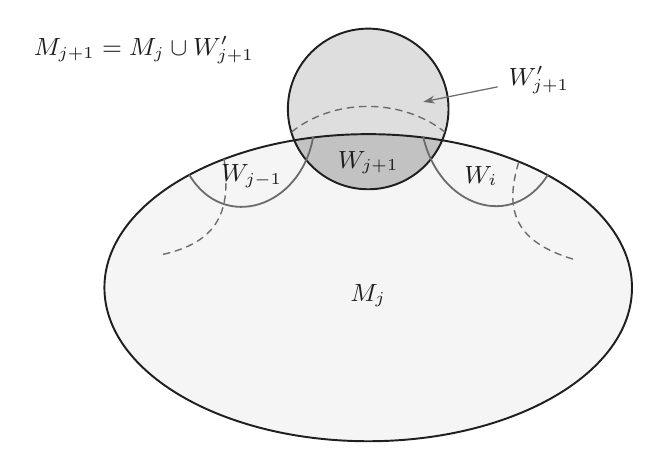
\begin{tikzpicture}[field/diagram, scale=1.0]
    % M_j and the enlarged Stein patch; their intersection is W_{j+1}.
    \fill[FieldPaper] (0,0) ellipse (3.35cm and 1.95cm);
    \fill[FieldRegion] (0,2.27) circle (1.02cm);
    \begin{scope}
        \clip (0,0) ellipse (3.35cm and 1.95cm);
        \fill[FieldEmphasis] (0,2.27) circle (1.02cm);
    \end{scope}
    \draw[field/boundary] (0,0) ellipse (3.35cm and 1.95cm);
    \draw[field/boundary] (0,2.27) circle (1.02cm);
    % Adjacent cover elements, bounded inside M_j by smooth arcs.
    \draw[field/secondary] (-2.27,1.43)
        .. controls (-1.83,0.70) and (-0.86,1.02) .. (-0.70,1.91);
    \draw[field/secondary] (0.70,1.91)
        .. controls (0.91,1.02) and (1.83,0.72) .. (2.28,1.43);
    \draw[field/hidden] (-0.97,1.98)
        .. controls (-0.43,2.41) and (0.42,2.41) .. (0.97,1.98);
    \draw[field/hidden] (-1.83,1.63)
        .. controls (-1.74,0.99) and (-1.89,0.58) .. (-2.62,0.42);
    \draw[field/hidden] (1.91,1.59)
        .. controls (1.72,0.96) and (1.88,0.58) .. (2.61,0.36);
    \node at (0,-0.10) {$M_j$};
    \node[inner sep=1pt] at (0,1.59) {$W_{j+1}$};
    \node[inner sep=1pt] at (-1.48,1.42) {$W_{j-1}$};
    \node[inner sep=1pt] at (1.43,1.42) {$W_i$};
    \node[anchor=west] at (1.67,2.64) {$W'_{j+1}$};
    \draw[field/leader] (1.64,2.55) -- (0.70,2.36);
    \node[anchor=east] at (-1.34,3.02) {$M_{j+1}=M_j\cup W'_{j+1}$};
\end{tikzpicture}

        \FieldCaption{II}{1}{}
    \end{minipage}
\end{center}
The covers $\mathcal W$, $\mathcal W'$ are Leray covers of $M_j$, $M_{j+1}$ for $\mathcal F$. Observe that any $p$-fold intersection of distinct elements of $\mathcal W$ is equal to a $p$-fold intersection of elements of $\mathcal W'$ provided only that $p>1$. Hence
\[
Z^p(\mathcal W,\mathcal F)\approx Z^p(\mathcal W',\mathcal F),\quad p\geq1.
\]
Therefore the natural restriction map $H^p(\mathcal W',\mathcal F)\to H^p(\mathcal W,\mathcal F)$ is surjective. Step 1 now follows by Leray's theorem.

\textbf{Step 2.} For $1\leq j\leq n$, set $W_j=V_j\cap M$, $W_j'=U_j\cap M_n$ and observe that $W_j$ is a relatively compact subset of $W_j'$. Choose Stein open subsets $W_{n+1},W_{n+1}',\ldots,W_p,W_p'$ of $M$ so that $W_j$ is a relatively compact subset of $W_j'$, $n+1\leq j\leq p$, and $\mathcal W=\{W_1,\ldots,W_p\}$, $\mathcal W'=\{W_1',\ldots,W_p'\}$ are open covers of $M$, $M_n$ respectively. Just as in the proof of the finiteness theorem of Cartan-Serre the restriction map
\[
R:Z^p(\mathcal W',\mathcal F)\to Z^p(\mathcal W,\mathcal F)
\]
is a compact operator between Fr\'echet spaces. From Step 1, the restriction map $H^p(\mathcal W',\mathcal F)\to H^p(\mathcal W,\mathcal F)$ is surjective, $p\geq1$, and so, for $p\geq1$, the map
\[
D\oplus R:C^{p-1}(\mathcal W,\mathcal F)\oplus Z^p(\mathcal W',\mathcal F)\to Z^p(\mathcal W,\mathcal F)
\]

% Source PDF page 180; printed page 171
is a surjective map between Fr\'echet spaces. Taking $A=D\oplus R$, $B=-0\oplus R$ in Schwartz' finiteness theorem we deduce the finiteness of $H^p(\mathcal W,\mathcal F)$, $p\geq1$.
\end{proof}
\begin{originaltheorem}{Theorem}{7.4.3 (Grauert \cite{bib:II:grauert-h:3})}\FieldTarget{theorem:7.4.3}{7.4.3}\IndexMark{idx-293}{holomorphic convexivity@Holomorphic convexivity!of s l p domain@of s.L.p. domain}
An S.L.p. domain\IndexMark{idx-275}{grauert theorem on holomorphic convexivity of s l p domains@Grauert theorem on holomorphic convexivity of s.L.p. domains} is holomorphically convex.
\end{originaltheorem}
\begin{proof}
Let $M$ be an S.L.p. domain in $\widehat M$. It is enough to show that given $p\in\partial M$, there exists $f\in A(M)$ which is unbounded on any sequence of points of $M$ converging to $p$. The method described in Exercise 2, \hyperref[sec:7:2]{\S2} will not work here as the ideal sheaf of an infinite discrete subset of $M$ does not extend to a coherent sheaf on $\widehat M$. Our proof follows that in R. Narasimhan \cite{bib:II:narasimhan-r:3}. As in the proof of Theorem~\ref{theorem:7.4.2} we suppose $M$ is defined by the $C^2$ function $\phi$. By Lemma~\ref{lemma:7.4.1}, we may choose an open neighbourhood $U$ of $p$ in $M$, biholomorphic map $\gamma:U\to E(r)$ and neighbourhood $N$ of $\phi\gamma^{-1}$ in $C_B^2(E(r))$ such that for all $\psi\gamma^{-1}\in N$, $D_r(\psi)=\{z:\psi(z)<0\}$ is Stein. Choose $\eta\in C_c^\infty(U)$ such that $\eta$ is positive, $\eta(p)>0$ and $(\phi-\eta)\gamma^{-1}\in N$. Let $\widetilde M=\{z\in\widehat M:\phi(z)-\eta(z)<0\}$. Certainly $\widetilde M\supset M$. As in the proof of Lemma~\ref{lemma:7.4.1}, there exists $F\in A(U)$ such that $F(p)=0$ and $F$ is non-zero in $D_r(\phi)$. Take the open cover $\mathcal U=\{U\cap\widetilde M,\widetilde M\setminus F^{-1}(0)\}$ of $\widetilde M$. Since the natural map $H^1(\mathcal U,\mathcal O_{\widetilde M})\to H^1(\widetilde M,\mathcal O_{\widetilde M})$ is injective (Exercise 4, \hyperref[sec:6:3]{\S3, Chapter 6}), and $\widetilde M$ is S.L.p., we have $\dim_{\mathbb C}H^1(\mathcal U,\mathcal O_{\widetilde M})<\infty$. Let $L$ denote the infinite dimensional linear subspace of $Z^1(\mathcal U,\mathcal O_{\widetilde M})$ defined by
\[
L=\left\{\sum_{j=1}^\infty c_jF^{-j}:c_j\in\mathbb C\text{ and all but finitely many }c_j\text{'s are zero}\right\}.
\]
Since $\dim_{\mathbb C}H^1(\mathcal U,\mathcal O_{\widetilde M})<\infty$, there exist elements of $L$ which are boundaries. Therefore we may find a combination
\[
G=\sum_{j=1}^n g_jF^{-j}\in L,
\]
with not all the $g_j$'s vanishing, such that $G=D(H)$, for some $H\in C^0(\mathcal U,\mathcal O_{\widetilde M})$. Hence there exist $H_0\in\mathcal O(U\cap\widetilde M)$, $H_1\in\mathcal O(\widetilde M\setminus F^{-1}(0))$ with $G=H_1-H_0$ on $(U\cap\widetilde M)\setminus F^{-1}(0)$. That is, we have
\[
H_1=H_0+\sum_{j=1}^n g_jF^{-1}\quad\text{on }(U\cap\widetilde M)\setminus F^{-1}(0).
\]
% Source PDF page 181; printed page 172
Clearly $f=H_1|M\in A(M)$ is unbounded on every sequence of points of $M$ converging to $p$.
\end{proof}
We may now give a solution to Levi's problem\IndexMark{idx-365}{levi s problem@Levi's problem}.
\begin{originaltheorem}{Theorem}{7.4.4}\FieldTarget{theorem:7.4.4}{7.4.4}
An S.L.p. domain of a Stein manifold is Stein.
\end{originaltheorem}
\begin{proof}
Immediate from Theorem~\ref{theorem:7.4.3}.
\end{proof}
\paragraph{Remarks.}
\begin{enumerate}[label=\arabic*.]
\item Suppose that $\Omega$ is a Levi pseudoconvex domain in $\mathbb C^n$ which is not S.L.p. Then it can easily be proved that $\Omega$ is the union of an increasing family of S.L.p. domains (see Oka \cite{bib:II:oka-k:1} or Gunning and Rossi \cite[Lemma 2, Section D, Chapter 10]{bib:II:gunning-r-c-and-rossi-h:1}). Hence, by Theorem~\ref{theorem:7.4.4}, $\Omega$ is the limit of an increasing family of domains of holomorphy and so, by a theorem of Behnke and Stein \cite{bib:II:behnke-h-and-stein-k:1}, a domain of holomorphy (see also Gunning and Rossi \cite[section D, Chapter 10]{bib:II:gunning-r-c-and-rossi-h:1}). This result was first obtained by Oka in case $n=2$ and then for general $n$ independently by Oka \cite{bib:II:oka-k:1}, Bremermann \cite{bib:II:bremermann-h-j:1} and Norguet \cite{bib:II:norguet-f:1}. Their result generalises to the case when $\Omega$ is a Levi pseudoconvex domain of a Riemann domain spread over $\mathbb C^n$ (see Gunning and Rossi \cite[section D, Chapter 10]{bib:II:gunning-r-c-and-rossi-h:1}). Moreover, it is not necessary to assume that the boundary of $\Omega$ is smooth. All that is required is that the function $-\log(d(z,\partial\Omega))$ is plurisubharmonic in $\Omega$ (see the above references and also H\"ormander \cite{bib:II:hormander-l:1}). It is not generally true that a Levi pseudoconvex domain of an arbitrary complex manifold is holomorphically convex. For an example of a non-holomorphically convex Levi pseudoconvex domain see Grauert \cite{bib:II:grauert-h:4} and also the survey article by Siu \cite{bib:II:siu-y-t:1}, especially \S7.
\item R. Narasimhan \cite{bib:II:narasimhan-r:4} has shown that if $M$ is a complex manifold then $\dim H^p(M,\mathcal F)<\infty$, $p\geq1$, for all coherent sheaves $\mathcal F$ on $M$ if and only if $M$ is holomorphically convex. The proof that finiteness of cohomology implies holomorphic convexity is similar to that indicated in Exercise 2, \hyperref[sec:7:2]{\S2} and makes use of the observation that the space of bounded infinite sequences of complex numbers is of infinite codimension in the space of all infinite complex sequences. The converse is much deeper and uses Grauert's direct image theorem together with results of H. Cartan \cite{bib:II:cartan-h:3} and Remmert \cite{bib:II:remmert-r:1} to the effect that if $M$ is holomorphically convex then $M$ possesses a maximal non-%
% Source PDF page 182; printed page 173
trivial compact analytic subset, $A$. Narasimhan proves that the inclusion $A\to M$ induces isomorphisms $H^p(A,\mathcal F_A)\to H^p(M,\mathcal F)$, $p\geq1$. The finiteness theorem of Cartan-Serre for compact analytic spaces then gives the result. In particular, $M$ will be Stein if and only if $M$ has no non-trivial compact analytic subsets. See Rossi \cite{bib:II:rossi-h:2} for a discussion of the case of S.L.p. domains.
\item Suppose $M$ is a strictly pseudoconvex manifold\IndexMark{idx-588}{strictly pseudoconvex manifold@Strictly pseudoconvex manifold}. That is, there exists a $C^\infty$ function $\phi:M\to\mathbb R$ such that $L(\phi)$ is everywhere positive definite and $M_a=\{z\in M:\phi(z)<a\}$ is relatively compact for all $a\in\mathbb R$. By Sard's theorem, $M_a$ is S.L.p. for a dense set $\Sigma\subset\mathbb R$ of values of $a$. Now it can be shown (see Gunning and Rossi \cite[Section C, Chapter 10]{bib:II:gunning-r-c-and-rossi-h:1}) that plurisubharmonic functions satisfy a maximal principle and so $M$ cannot have any non-trivial compact analytic subsets. It follows from Remark 2 that $M_a$ is Stein, $a\in\Sigma$. Thus we have expressed $M$ as a union of an increasing family of Stein manifolds parametrized by points in a dense subset of $\mathbb R$. It is shown in Docquier and Grauert \cite{bib:II:docquier-f-and-grauert-h:1} that this is enough to prove $M$ Stein. See also Siu \cite{bib:II:siu-y-t:1} and note that it is not generally true that an increasing union of Stein open sets, parametrized by the positive integers, need be Stein. Of course the union will be Stein if all the sets are domains in $\mathbb C^n$ or a Riemann domain (see Remark 1). If they are all subdomains of a Stein manifold it is not yet known whether their union must be Stein (see also Markoe \cite{bib:II:markoe-a:1}). We shall prove in Chapter 11 that every strictly pseudoconvex manifold is Stein. Our proof will depend on the existence theory for the $\bar\partial$-operator and follows the approach of Kohn \cite{bib:II:kohn-j-j:1}, Andreotti-Vesentini \cite{bib:II:andreotti-a-and-vesentini-e:1}, H\"ormander \cite{bib:II:hormander-l:1} and Vesentini \cite{bib:II:vesentini-e:1}.
\end{enumerate}
\paragraph{Exercise.} Let $M$ be an S.L.p. domain in the complex manifold $\widehat M$ and suppose that $M$ has $C^2$ defining function $\phi$. Show
\begin{enumerate}[label=\alph*)]
\item There exists $C>0$ such that $M_c=\{x\in M:\phi(x)<-c\}$ is S.L.p. for $0\leq c<C$.
\item[b)*] If $M$ has no non-trivial compact analytic subvarieties then $M_c$ is Stein, $0<c<C$ (See Rossi \cite{bib:II:rossi-h:1} and note that we do not need to assume a maximal principle for strictly psh functions).
\end{enumerate}
% Source PDF page 183; printed page 174
\section{Coherent sheaves on projective space}\label{sec:7:5}
In this section we shall prove theorems A and B of Serre for coherent sheaves on projective space. These fundamental theorems play a similar r\^ole in the theory of projective varieties to that of Cartan's theorems A and B in Stein manifold theory.

Throughout this section $\mathcal U=\{U_i\}$ will denote the standard open cover of $\mathbb P^n(\mathbb C)$ by the open sets $U_i=\{(z_0,\ldots,z_n):z_i\ne0\}$, $0\leq i\leq n$. Suppose that $\mathcal F$ is a coherent sheaf on $\mathbb P^n(\mathbb C)$. Since each $U_i$ is biholomorphic to $\mathbb C^n$ and is therefore Stein, $\mathcal U$ is a Leray cover of $\mathbb P^n(\mathbb C)$ for $\mathcal F$. It follows immediately from Leray's theorem that
\[
H^p(\mathbb P^n(\mathbb C),\mathcal F)=0,\quad p>n.
\]
Let $H$ denote the hyperplane section bundle\IndexMark{idx-198}{divisors@Divisors!complex projective space@complex projective space} of $\mathbb P^n(\mathbb C)$. Relative to the cover $\mathcal U$, $H$ has transition functions $\phi_{ij}=z_j/z_i$. For $m\in\mathbb Z$, we let $H^m$ denote the holomorphic line bundle with transition functions $(z_j/z_i)^m$ on $U_{ij}$. We may regard $H^m$ as the line bundle associated to the divisor $z_0^m=0$. That is, if we let $\mathbb P^{n-1}(\mathbb C)\subset\mathbb P^n(\mathbb C)$ denote the hyperplane $z_0=0$, we have $H^m=[m.\mathbb P^{n-1}(\mathbb C)]$. With this convention, $H^m$ has the ``canonical'' section $s^m$ given locally by $s_i^m=(z_0/z_i)^m$ and $\operatorname{div}(s^m)=m.\mathbb P^{n-1}(\mathbb C)$.

As is conventional, we let $\mathcal O(m)$ denote the sheaf of germs of holomorphic sections of $H^m$, $m\in\mathbb Z$.
\begin{originaltheorem}{Lemma}{7.5.1}\FieldTarget{lemma:7.5.1}{7.5.1}
Let $\Sigma$ be a hyperplane in $\mathbb P^n(\mathbb C)$. For $m\in\mathbb Z$, we have a non-zero $\mathcal O$-morphism
\[
\phi_\Sigma:\mathcal O(m)\to\mathcal O(m+1)
\]
satisfying $\phi_{\Sigma,z}=0$ if and only if $z\in\Sigma$. In particular, $\phi_\Sigma$ restricts to an isomorphism of $\mathcal O(m)$ with $\mathcal O(m+1)$ over $\mathbb P^n(\mathbb C)\setminus\Sigma$.
\end{originaltheorem}
\begin{proof}
Let $\Sigma$ have equation $s(z_0,\ldots,z_n)=0$. Define $\phi_\Sigma(f)=s_zf$, $f\in\mathcal O(m)_z$.
\end{proof}
\paragraph{Remark.} The morphism $\phi_\Sigma$ is given locally by $\phi_\Sigma(f_i)=f_is/z_i$, $f_i\in\mathcal O(m)(U_i)$.
% Source PDF page 184; printed page 175
Let $P^{(m)}(\mathbb C^{n+1})$ denote the space of homogeneous polynomials of degree $m$ on $\mathbb C^{n+1}$. Then (Proposition~\ref{proposition:5.9.2}),
\[
\begin{aligned}
H^0(\mathbb P^n(\mathbb C),\mathcal O(m))&\approx P^{(m)}(\mathbb C^{n+1}),\quad m\geq0\\
&=0,\quad m<0.
\end{aligned}
\]
\begin{originaltheorem}{Theorem}{7.5.2}\FieldTarget{theorem:7.5.2}{7.5.2}\IndexMark{idx-098}{cohomology of o m sheaves on p n c@Cohomology of $O(m)$ sheaves on $\mathbb{P}^n(\mathbb{C})$}
\begin{enumerate}[label=\arabic*.]
\item For $m\geq0$, we have
\[
\begin{aligned}
H^p(\mathbb P^n(\mathbb C),\mathcal O(m))&=0,\quad p\ne0\\
&\approx P^{(m)}(\mathbb C^{n+1}),\quad p=0.
\end{aligned}
\]
\item For $m<0$, we have
\[
\begin{aligned}
H^p(\mathbb P^n(\mathbb C),\mathcal O(m))&=0,\quad p\ne n\\
&\approx P^{(-m-n-1)}(\mathbb C^{n+1}),\quad p=n.
\end{aligned}
\]
\end{enumerate}
\end{originaltheorem}
\begin{proof}
Since we have already covered the cases $p=0$, $p>n$, we shall assume from now on that $1\leq p\leq n$. Let us start by considering the case $m=0$. Suppose $c\in Z^p(\mathcal U,\mathcal O)$. Then $c=\{c(s)=c(s_0,\ldots,s_p)\}$, where $c(s):U\to\mathbb C$ is holomorphic and $s=(s_0,\ldots,s_p)$ is a $(p+1)$-tuple of (distinct) integers lying between $0$ and $n$. We may regard each $c(s)$ as a holomorphic function on $U_s\subset\mathbb C^{n+1}$ which is homogeneous of degree zero. By Theorem~\ref{theorem:2.1.10}, we may take Laurent expansions of the $c(s)$. Thus
\[
\begin{aligned}
c(s)(z_0,\ldots,z_n)&=\sum_{r_0+\cdots+r_n=0}c(s)_{r_0\cdots r_n}z_0^{r_0}\cdots z_n^{r_n}\\
&=\sum_{|r|=0}c(s)_rz^r,\quad\text{using multi-index notation.}
\end{aligned}
\]
Observe that the coefficient $c(s)_{r_0\cdots r_n}$ will be zero if any $r_j<0$ with $j\notin\{s_0,\ldots,s_p\}$. Define
\[
a(s_0,\ldots,s_{p-1})=\frac1{n-p+1}\sum{}'c(j,s_0,\ldots,s_{p-1})^+,
\]
% Source PDF page 185; printed page 176
where $\sum{}'$ denotes the sum over all $j\notin\{s_0,\ldots,s_{p-1}\}$ and $c(j,s_0,\ldots,s_{p-1})^+$ is the holomorphic function on $U_{s_0}\cap\cdots\cap U_{s_{p-1}}$ with Laurent series
\[
\sum_{\substack{|r|=0\\r_j\geq0}}c(j,s_0,\ldots,s_{p-1})_rz^r.
\]
That is, we omit terms from the Laurent expansion of $c(j,s_0,\ldots,s_{p-1})$ having $r_j<0$. Our construction defines an element $a\in C^{p-1}(\mathcal U,\mathcal O)$. Now
\[
\begin{aligned}
(Da)_{s_0\cdots s_p}
&=\frac1{n-p+1}\left(\sum{}'\bigl(c(j,s_1,s_2,\ldots,s_p)-\cdots\pm c(j,s_0,\ldots,s_{p-1})\bigr)^+\right)\\
&=\frac1{n-p+1}\left(\sum{}'c(s_0,\ldots,s_p)\right)^+,\quad\text{since }Dc=0\\
&=c(s_0,\ldots,s_p).
\end{aligned}
\]
We have shown that $Z^p(\mathcal U,\mathcal O)=DC^{p-1}(\mathcal U,\mathcal O)$ and so $H^p(\mathcal U,\mathcal O)=0$, $p>0$.

Exactly the same proof shows that if $m>0$ then $H^p(\mathcal U,\mathcal O(m))=0$, $p>0$. Indeed, the only difference is that a cochain will now be a collection of holomorphic functions which are homogeneous of degree $m$. The same proof also works for $m<0$ provided that $p<n$. We conclude by considering the case $p=n$, $m<0$. Suppose $c\in Z^n(\mathcal U,\mathcal O(m))$. Then
\[
c:U_{01\cdots n}\to\mathbb C
\]
is holomorphic and homogeneous of degree $m$. Thus
\[
c(z_0,\ldots,z_n)=\sum_{|r|=m}c_rz^r.
\]
Write $c=C_0+C_1$, where $C_0$ is the sum over all terms $c_{r_0\cdots r_n}z_0^{r_0}\cdots z_n^{r_n}$ where at least one index $r_j$ is positive and $C_1$ is the sum over terms such that every index $r_j$ is negative. Notice that $C_1=0$ if $-m\leq n$. As above it is easily seen that $C_0=Da$ for some $(n-1)$-cochain $a$. A simple Laurent series argument shows that a non-zero $C_1$ can never be a coboundary. So suppose $m\leq-n-1$ and set
% Source PDF page 186; printed page 177
\[
E=\left\{\sum_{|r|=m}c_rz^r:c_r\in\mathbb C,\ \text{every index }r_j<0\right\}.
\]
By what we have shown above $E\approx H^n(\mathcal U,\mathcal O(m))$. Given $c\in E$, we may write
\[
c=(z_0\cdots z_n)^{-1}\sum_{\substack{r_0,\ldots,r_n\leq0\\r_0+\cdots+r_n=m+m+1}}c_rz_0^{r_0+1}\cdots z_n^{r_n+1}.
\]
It follows that $H^n(\mathcal U,\mathcal O(m))\approx P^{(-m-n-1)}(\mathbb C^{n+1})$ where the isomorphism is given explicitly by mapping $P\in P^{(-m-n-1)}(\mathbb C)$ to
\[
c(z_0,\ldots,z_n)=(z_0\cdots z_n)^{-1}P(z_0^{-1},\ldots,z_n^{-1}).
\]
\end{proof}
\paragraph{Remark.} For an alternative proof of Theorem~\ref{theorem:7.5.2}, using non-trivial facts from the Hodge theory of K\"ahler manifolds, see Seminar 18 by Serre in H. Cartan \cite{bib:II:cartan-h:2}.

Given a coherent sheaf $\mathcal F$ on $\mathbb P^n(\mathbb C)$ we let
\[
\mathcal F(m)=\mathcal F\otimes_{\mathcal O}\mathcal O(m),\quad m\in\mathbb Z.
\]
We call $\mathcal F(m)$ the sheaf $\mathcal F$ ``twisted by\IndexMark{idx-624}{twisted sheaves on projective space@Twisted sheaves on projective space} $\mathcal O(m)$''. One feature of twisting is that we expect $\dim_{\mathbb C}H^0(\mathbb P^n(\mathbb C),\mathcal F(m))$ to be an increasing function of $m$. To explain why this should be so, let us consider the case when $\mathcal F$ is the sheaf of sections of a holomorphic vector bundle $E$. We claim that $H^0(\mathbb P^n(\mathbb C),E(m))\cong\{s\in\mathcal M(E):\operatorname{div}(s)+m.\mathbb P^{n-1}(\mathbb C)\geq0\}$. Certainly it follows from this isomorphism that $\dim_{\mathbb C}H^0(\mathbb P^n(\mathbb C),E(m))$ is an increasing function of $m$. Suppose that $E$ has transition functions $\phi_{ab}$ relative to a cover $\mathcal W$ of $\mathbb P^n(\mathbb C)$ where we suppose that $\mathcal W$ is a refinement of $\mathcal U$. Let $s\in\mathcal M^*(E)$ and $\operatorname{div}(s)+m.\mathbb P^{n-1}(\mathbb C)\geq0$. If $s_a\in\mathcal M^*(W_a)$ is the local representative of $s$ on $W_a\subset U_{i(a)}$, we have
\[
(z_0/z_{i(a)})^ms_a\in A(W_a).
\]
Clearly if $W_b\subset U_{i(b)}$, we have
\[
\phi_{ab}(z_{i(b)}/z_{i(a)})^m(z_0/z_{i(b)})^ms_b=(z_0/z_{i(a)})^ms_a\quad\text{on }W_{ab}.
\]
% Source PDF page 187; printed page 178
Therefore $\{(z_0/z_{i(a)})^ms_a\}$ defines a holomorphic section of $E(m)$. Reversing the argument shows that every holomorphic section of $E(m)$ gives rise to a meromorphic section of $E$ such that $\operatorname{div}(s)+m.\mathbb P^{n-1}(\mathbb C)\geq0$. Of course, our argument depended on being able to show that $E$ admits at least one non-trivial meromorphic section.

\paragraph{Remark.} We should point out that a holomorphic vector bundle $E$ on $\mathbb P^n(\mathbb C)$ always restricts to a holomorphically trivial bundle over $U_i$, $0\leq i\leq n$, Serre \cite{bib:II:serre-j-p:2}. This fact also follows from a general and difficult theorem of Grauert to the effect that a holomorphic vector bundle on a Stein manifold is holomorphically trivial if and only if it is topologically trivial. See also Adams and Griffiths \cite{bib:II:adams-j-f-and-griffiths-p:1} for a proof that holomorphic vector bundles over polydiscs in $\mathbb C^n$ are holomorphically trivial as well as references and discussion concerning Grauert's theorems.
\begin{originaltheorem}{Theorem}{7.5.3 (Theorems A and B of Serre)}\IndexMark{idx-546}{serre theorems a and b@Serre theorems A and B}\FieldTarget{theorem:7.5.3}{7.5.3}
Let $\mathcal F$ be a coherent sheaf on $\mathbb P^n(\mathbb C)$. Then there exists $m_0=m_0(\mathcal F)\in\mathbb Z$ such that
\begin{enumerate}[label=\Alph*.]
\item For each $z\in\mathbb P^n(\mathbb C)$, $H^0(\mathbb P^n(\mathbb C),\mathcal F(m))$ generates $\mathcal F(m)_z$ as a $\mathcal G_z$-module, $m\geq m_0$.
\item For $m\geq m_0$, $H^p(\mathbb P^n(\mathbb C),\mathcal F(m))=0$, $p\geq1$.
\end{enumerate}
\end{originaltheorem}
\begin{proof}[Proof (Seminar 19 by Serre, H. Cartan \cite{bib:II:cartan-h:2})]
We start by looking at some special cases. Suppose $\mathcal F\cong\mathcal O(q)$. Take $m_0=-q$. Since $\mathcal O(q)(m)=\mathcal O(q+m)$, we see immediately from Theorem~\ref{theorem:7.5.2} that $H^p(\mathbb P^n(\mathbb C),\mathcal F(m))=0$, $p\geq1$, $m\geq m_0$. Clearly for all $z\in\mathbb P^n(\mathbb C)$, $H^0(\mathbb P^n(\mathbb C),\mathcal F(m))$ generates $\mathcal F(m)_z$, $m\geq m_0$. Since cohomology commutes with direct sums, A and B hold whenever $\mathcal F\cong\bigoplus_{i=1}^k\mathcal O(a_i)$ and we may take $m_0=-\min\{a_i\}$.

We prove the theorem in general by an induction on $n$. Let $A_n$, $B_n$ denote statements A and B for dimension $n$. We shall show that $A_{n-1}$ and $B_{n-1}$ imply $A_n$ and $A_n$ implies $B_n$. The Theorem is, of course, trivial for $n=0$.

\textbf{Step 1.} $A_{n-1}$ and $B_{n-1}$ imply $A_n$. Let $z\in\mathbb P^n(\mathbb C)$ and choose any hyperplane $\Sigma\subset\mathbb P^n(\mathbb C)$ not containing $z$. For $m\in\mathbb Z$, let

% Source PDF page 188; printed page 179. Continuation of the proof of Theorem~\ref{theorem:7.5.3}.
\[
\widetilde\phi_\Sigma=\operatorname{id}\otimes\phi_\Sigma:\mathcal{F}(m)\longrightarrow\mathcal{F}(m+1),
\]
where $\phi_\Sigma$ is the map given by Lemma~\ref{lemma:7.5.1}. Observe that $\widetilde\phi_\Sigma$ restricts to an isomorphism of $\mathcal{F}(m)$ with $\mathcal{F}(m+1)$ over $\mathbb{P}^n(\mathbb{C})\setminus\Sigma$. Suppose $H^0(\mathbb{P}^n(\mathbb{C}),\mathcal{F}(m_0))$ generates $\mathcal{F}(m_0)_z$. Then $H^0(\mathbb{P}^n(\mathbb{C}),\mathcal{F}(m))$ generates $\mathcal{F}(m)_z$ for $m\geq m_0$. Indeed, $\widetilde\phi_\Sigma^{m-m_0}:\mathcal{F}(m_0)\to\mathcal{F}(m)$ restricts to an isomorphism over $\mathbb{P}^n(\mathbb{C})\setminus\Sigma$ and so maps any set of generators for $\mathcal{F}(m_0)_z$ to a set of generators for $\mathcal{F}(m)_z$. Let $A_n(z)$ (respectively $A'_n(z)$) be the statement ``There exists $m_0=m_0(\mathcal{F},z)$ such that $H^0(\mathbb{P}^n(\mathbb{C}),\mathcal{F}(m_0))$ (respectively $H^0(\mathbb{P}^n(\mathbb{C}),\mathcal{F}(m))$) generates $\mathcal{F}(m_0)_z$ (respectively $\mathcal{F}(m)_z$, $m\geq m_0$)''. By the coherence of $\mathcal{F}$, $A_n(z)$ implies $A_n(y)$ for $y$ in some open neighbourhood of $z$. Since $A_n(y)$ implies $A'_n(y)$, it follows from the compactness of $\mathbb{P}^n(\mathbb{C})$ that $A_n(z)$ for all $z\in\mathbb{P}^n(\mathbb{C})$ implies $A_n$. Therefore it is enough to prove that $A_{n-1}$ and $B_{n-1}$ imply $A_n(z)$.

Without loss of generality suppose $z\in\mathbb{P}^{n-1}(\mathbb{C})\subset\mathbb{P}^n(\mathbb{C})$. Set $\phi=\widetilde\phi_{\mathbb{P}^{n-1}(\mathbb{C})}:\mathcal{F}(-1)\to\mathcal{F}$ and let
\[
\begin{aligned}
\mathcal{K}&=\operatorname{Ker}\phi:\mathcal{F}(-1)\to\mathcal{F}\\
\mathcal{G}&=\operatorname{Coker}\phi:\mathcal{F}(-1)\to\mathcal{F}.
\end{aligned}
\]
We have the exact sequence
\[
0\to\mathcal{K}\to\mathcal{F}(-1)\xrightarrow{\phi}\mathcal{F}\to\mathcal{G}\to0.
\]
Tensoring with $O(m)$ we obtain the exact sequence
\[
0\to\mathcal{K}(m)\to\mathcal{K}(m-1)\xrightarrow{\phi_m}\mathcal{F}(m)\to\mathcal{G}(m)\to0.
\]
% Source prints K(m-1) here, rather than F(m-1); retained verbatim.
Since $\phi_m|U_0$ is an isomorphism we see that $\mathcal{K}_{U_0}=\mathcal{G}_{U_0}=0$. Let $i$ denote the inclusion map of $\mathbb{P}^{n-1}(\mathbb{C})$ in $\mathbb{P}^n(\mathbb{C})$. For any sheaf $\mathcal{H}$ on $\mathbb{P}^n(\mathbb{C})$ we let $\mathcal{H}^*=i^{-1}\mathcal{H}$ denote the restriction of $\mathcal{H}$ to $\mathbb{P}^{n-1}(\mathbb{C})$. Observe that $\mathcal{I}_{\mathbb{P}^{n-1}(\mathbb{C})}\subset\mathcal{O}_{\mathbb{P}^n(\mathbb{C})}$ acts trivially on $\mathcal{K}$ and $\mathcal{G}$. Indeed if $s_z\in\mathcal{I}_{\mathbb{P}^{n-1}(\mathbb{C})}$, $f_z\in\mathcal{K}$, then $s_zf_z=0$ since $\mathcal{K}=\operatorname{Ker}(\phi)$. Similarly for $\mathcal{G}$ since $\mathcal{G}=\operatorname{Coker}(\phi)$. Hence $\mathcal{K}^*$, $\mathcal{G}^*$ have the natural structure of $\mathcal{O}_{\mathbb{P}^{n-1}(\mathbb{C})}=\mathcal{O}_{\mathbb{P}^n(\mathbb{C})}^*/\mathcal{I}_{\mathbb{P}^{n-1}(\mathbb{C})}^*$-modules and the reader may easily verify that $\mathcal{K}^*$, $\mathcal{G}^*$ are coherent $\mathcal{O}_{\mathbb{P}^{n-1}(\mathbb{C})}$-modules. Moreover, it is clear that $\mathcal{K}(m)^*\approx\mathcal{K}^*(m)$, $\mathcal{G}(m)^*\approx\mathcal{G}^*(m)$, $m\in\mathbb{Z}$.

% Source PDF page 189; printed page 180.
By Exercise 12, \hyperref[sec:6:3]{\S3, Chapter 6},
\[
H^p(\mathbb{P}^n(\mathbb{C}),\mathcal{K}(m))=H^p(\mathbb{P}^{n-1}(\mathbb{C}),\mathcal{K}(m)^*),\quad p\geq0,
\]
similarly for $\mathcal{G}(m)$. Applying our inductive assumption to $\mathcal{K}^*$, $\mathcal{G}^*$, there exists $m_1\in\mathbb{Z}$ such that for $p\geq1$
\[
\begin{aligned}
H^p(\mathbb{P}^n(\mathbb{C}),\mathcal{K}(m))&=H^p(\mathbb{P}^{n-1}(\mathbb{C}),\mathcal{K}^*(m))=0,\quad m\geq m_1\\
H^p(\mathbb{P}^n(\mathbb{C}),\mathcal{G}(m))&=H^p(\mathbb{P}^{n-1}(\mathbb{C}),\mathcal{G}^*(m))=0,\quad m\geq m_1.
\end{aligned}
\]
We have the short exact sequences
\[
\begin{aligned}
0&\to\mathcal{K}(m)\to\mathcal{F}(m-1)\to\operatorname{Im}(\phi_{m-1})\to0\\
0&\to\operatorname{Im}(\phi_{m-1})\to\mathcal{F}(m)\to\mathcal{G}(m)\to0.
\end{aligned}
\]
Taking the cohomology sequences of these short exact sequences we obtain the exact sequences
\[
\begin{aligned}
H^1(\mathbb{P}^n(\mathbb{C}),\mathcal{F}(m-1))&\to H^1(\mathbb{P}^n(\mathbb{C}),\operatorname{Im}(\phi_{m-1}))\to H^2(\mathbb{P}^n(\mathbb{C}),\mathcal{K}(m))\\
H^1(\mathbb{P}^n(\mathbb{C}),\operatorname{Im}(\phi_{m-1}))&\to H^1(\mathbb{P}^n(\mathbb{C}),\mathcal{F}(m))\to H^1(\mathbb{P}^n(\mathbb{C}),\mathcal{G}(m)).
\end{aligned}
\]
Since $H^1(\mathbb{P}^n(\mathbb{C}),\mathcal{G}(m))$, $H^2(\mathbb{P}^n(\mathbb{C}),\mathcal{K}(m))=0$, $m\geq m_1$, we see that
\[
\begin{aligned}
\dim_{\mathbb{C}}H^1(\mathbb{P}^n(\mathbb{C}),\mathcal{F}(m-1))&\geq\dim_{\mathbb{C}}H^1(\mathbb{P}^n(\mathbb{C}),\operatorname{Im}(\phi_{m-1}))\\
&\geq\dim_{\mathbb{C}}H^1(\mathbb{P}^n(\mathbb{C}),\mathcal{F}(m)),
\end{aligned}
\]
for $m\geq m_1$. Hence $\dim_{\mathbb{C}}H^1(\mathbb{P}^n(\mathbb{C}),\mathcal{F}(m))$ is a decreasing function of $m$, $m\geq m_1$. But now by the finiteness theorem of Cartan--Serre, $\dim_{\mathbb{C}}H^1(\mathbb{P}^n(\mathbb{C}),\mathcal{F}(m))<\infty$, and so we deduce that $\dim_{\mathbb{C}}H^1(\mathbb{P}^n(\mathbb{C}),\mathcal{F}(m))$ is independent of $m$ for $m>m_2$, say. In particular, for $m\geq m_2$ we have
\[
\begin{aligned}
\dim_{\mathbb{C}}H^1(\mathbb{P}^n(\mathbb{C}),\mathcal{F}(m-1))&=\dim_{\mathbb{C}}H^1(\mathbb{P}^n(\mathbb{C}),\operatorname{Im}(\phi_{m-1}))\\
&=\dim_{\mathbb{C}}H^1(\mathbb{P}^n(\mathbb{C}),\mathcal{F}(m)).
\end{aligned}
\]
Since the surjective homomorphism $H^1(\mathbb{P}^n(\mathbb{C}),\operatorname{Im}(\phi_{m-1}))\to H^1(\mathbb{P}^n(\mathbb{C}),\mathcal{F}(m))$ is between spaces of the same finite dimension, it must be injective, $m\geq m_2$. Therefore, from the cohomology sequence we see that $H^0(\mathbb{P}^n(\mathbb{C}),\mathcal{F}(m))\to H^0(\mathbb{P}^n(\mathbb{C}),\mathcal{G}(m))$ is surjective, $m\geq m_2$. But $H^0(\mathbb{P}^n(\mathbb{C}),\mathcal{G}(m))=H^0(\mathbb{P}^{n-1}(\mathbb{C}),\mathcal{G}^*(m))$ and so by $A_{n-1}$ we see that $H^0(\mathbb{P}^n(\mathbb{C}),\mathcal{G}(m))$ generates $\mathcal{G}^*(m)_z=\mathcal{G}(m)_z$ for $m\geq m_0$, where we may suppose $m_0\geq m_2$. In particular, $H^0(\mathbb{P}^n(\mathbb{C}),\mathcal{F}(m))$ generates $\mathcal{G}(m)_z$ for
% Source PDF page 190; printed page 181.
$m\geq m_0$. We claim that for $m\geq m_0$, $H^0(\mathbb{P}^n(\mathbb{C}),\mathcal{F}(m))$ generates $\mathcal{F}(m)_z$. Suppose $z\in U_i$, $i\ne0$. Let $\psi:\mathcal{F}\to\mathcal{F}(1)$ be the homomorphism defined by $\psi(f)=z_i f$. As described above, $\psi^{-m}$ restricts to an isomorphism of $\mathcal{F}(m)_{U_i}$ with $\mathcal{F}_{U_i}$. Under this identification of $\mathcal{F}(m)_{U_i}$ with $\mathcal{F}_{U_i}$, the map $\phi$ corresponds to multiplication by $t_0=z_0/z_i$ and $\mathcal{G}(m)_z$ is therefore identified with $\mathcal{F}_z/t_0\mathcal{F}_z$. Let $M_z\subset\mathcal{F}_z$ be the submodule generated by the elements of $H^0(\mathbb{P}^n(\mathbb{C}),\mathcal{F}(m))$. Since $\mathcal{G}(m)_z$ is generated by the elements of $H^0(\mathbb{P}^n(\mathbb{C}),\mathcal{F}(m))$, $m\geq m_0$, the image of $M_z$ in $\mathcal{F}_z/t_0\mathcal{F}_z$ is the whole of $\mathcal{F}_z/t_0\mathcal{F}_z$. That is, $\mathcal{F}_z=t_0\mathcal{F}_z+M_z$. Since $t_0\in\mathfrak{m}_z\subset\mathcal{O}_z$, it follows from Nakayama's lemma that $\mathcal{F}_z=M_z$.

\paragraph{Step 2.} $A_n$ implies $B_n$.

For $p>n$, we have already shown that $H^p(\mathbb{P}^n(\mathbb{C}),\mathcal{F}(m))=0$ for all $m$. We prove $B_n$ by decreasing induction on $p$. So suppose that for every coherent sheaf $\mathcal{F}$ on $\mathbb{P}^n(\mathbb{C})$ there exists $m_0=m_0(\mathcal{F},p)$ such that $H^{p+1}(\mathbb{P}^n(\mathbb{C}),\mathcal{F}(m))=0$, $m\geq m_0$. By $A_n$ there exists $m\in\mathbb{Z}$ such that $H^0(\mathbb{P}^n(\mathbb{C}),\mathcal{F}(m))$ generates $\mathcal{F}(m)_z$ for all $z\in\mathbb{P}^n(\mathbb{C})$. Choose a basis $s_1,\ldots,s_k$ of $H^0(\mathbb{P}^n(\mathbb{C}),\mathcal{F}(m))$. We have the exact sequence
\[
0\to\mathcal{K}\to\mathcal{O}^k\xrightarrow{s}\mathcal{F}(m)\to0,
\]
where $s=(s_1,\ldots,s_k)$ and $\mathcal{K}=\operatorname{Ker}(s)$. Tensoring by $O(q)$ yields the exact sequence
\[
0\to\mathcal{K}(q)\to\mathcal{O}^k(q)\to\mathcal{F}(m+q)\to0
\]
and corresponding portion of the cohomology sequence
\[
H^p(\mathbb{P}^n(\mathbb{C}),\mathcal{O}^k(q))\to H^p(\mathbb{P}^n(\mathbb{C}),\mathcal{F}(m+q))\to H^{p+1}(\mathbb{P}^n(\mathbb{C}),\mathcal{K}(q)).
\]
By the special case of B described at the beginning of the proof, $H^p(\mathbb{P}^n(\mathbb{C}),\mathcal{O}^k(q))=0$ for $p>0$, $q\geq0$. By our inductive assumption, $H^{p+1}(\mathbb{P}^n(\mathbb{C}),\mathcal{K}(q))=0$ for sufficiently large $q$. Hence $H^p(\mathbb{P}^n(\mathbb{C}),\mathcal{F}(m+q))=0$ for sufficiently large $q$. This completes the inductive step and the proof of the theorem.
\end{proof}
% Source PDF page 191; printed page 182.
\paragraph{Remark.} The reader should note the crucial r\^ole played by the finiteness theorem of Cartan--Serre in the proof of Theorem~\ref{theorem:7.5.3}. In \hyperref[sec:7:6]{\S6}, we give another proof of Theorem~\ref{theorem:7.5.3} depending on Grauert's finiteness theorem.

Now for some applications of Serre's theorem.

\begin{originaltheorem}{Theorem}{7.5.4}\FieldTarget{theorem:7.5.4}{7.5.4}
Every holomorphic vector bundle $E$ on $\mathbb{P}^n(\mathbb{C})$ has a non-trivial meromorphic section\IndexMark{idx-305}{holomorphic vector bundles on p n c@Holomorphic vector bundles on $\mathbb{P}^n(\mathbb{C})$!existence of non trivial meromorphic sections@existence of non-trivial meromorphic sections}\IndexMark{idx-395}{meromorphic section@Meromorphic section!on p n c@on $\mathbb{P}^n(\mathbb{C})$}.
\end{originaltheorem}
\begin{proof}
By statement A of Theorem~\ref{theorem:7.5.3}, there exists $m_0$ such that $H^0(\mathbb{P}^n(\mathbb{C}),\underline{E}(m_0))$ generates $\underline{E}(m_0)_z$ for all $z\in\mathbb{P}^n(\mathbb{C})$. In particular, $\dim_{\mathbb{C}}H^0(\mathbb{P}^n(\mathbb{C}),\underline{E}(m_0))\geq1$. But as we showed earlier,
\[
H^0(\mathbb{P}^n(\mathbb{C}),\underline{E}(m_0))\cong\{s\in \mathcal{M}(E):\operatorname{div}(s)+m_0.\mathbb{P}^{n-1}(\mathbb{C})\geq0\}.
\]
\end{proof}
\paragraph{Remark.} Of course, we can prove much more than that $E$ has a non-trivial meromorphic section. Using statement B, we can show that for any $v\in E_z$, there exists $s\in \mathcal{M}^*(E)$ such that $s(z)=v$. See the exercises at the end of the section.

\begin{originaltheorem}{Theorem}{7.5.5}\FieldTarget{theorem:7.5.5}{7.5.5}
(Chow's theorem\IndexMark{idx-084}{chow s theorem@Chow's theorem}). Every analytic subset of $\mathbb{P}^n(\mathbb{C})$ is algebraic.
\end{originaltheorem}
\begin{proof}
Let $X$ be an analytic subset of $\mathbb{P}^n(\mathbb{C})$ with ideal sheaf $\mathcal{I}$. Then $\mathcal{I}$ is coherent subsheaf of $\mathcal{O}$ (see \hyperref[sec:7:1]{\S1} for discussion and references). We prove: Given $z\in\mathbb{P}^n(\mathbb{C})\setminus X$, there exists a homogeneous polynomial $p=p(z_0,\ldots,z_n)$ which vanishes on $X$ and does not vanish at $x$. Granted this, we consider the set of all homogeneous polynomials which vanish on $X$. The common zero locus of these polynomials is $X$ and by the Hilbert basis theorem we may choose a finite subset of these polynomials with common zero locus $X$.

Suppose then that $\mathcal{I}_z$ denotes the ideal sheaf of $X\cup\{z\}$. For $m\in\mathbb{Z}$, we have the exact sequence
\[
0\to\mathcal{I}_z(m)\to\mathcal{I}\to\mathbb{C}(z)(m)\to0,
\]
% The source prints I without a twist in this display; retained.
where $\mathbb{C}(z)$ is the skyscrapper sheaf supported at $z$. Note that $\mathbb{C}(z)(m)=\mathbb{C}(z)$. By B of Theorem~\ref{theorem:7.5.3}, there exists $m_0$ such that $H^1(\mathbb{P}^n(\mathbb{C}),\mathcal{I}_z(m))=0$, $m\geq m_0$. Taking the cohomology sequence of our short exact sequence we obtain for $m\geq m_0$ the exact sequence
% Source PDF page 192; printed page 183.
\[
H^0(\mathbb{P}^n(\mathbb{C}),\mathcal{I}(m))\to H^0(\mathbb{P}^n(\mathbb{C}),\mathbb{C}(z)(m))\to0.
\]
Now $H^0(\mathbb{P}^n(\mathbb{C}),\mathbb{C}(z)(m))\cong\mathbb{C}$ and so there exists $p\in H^0(\mathbb{P}^n(\mathbb{C}),\mathcal{I}(m))$ such that $p(z)\ne0$. But since $\mathcal{I}\subset\mathcal{O}$, it follows that $H^0(\mathbb{P}^n(\mathbb{C}),\mathcal{I}(m))$ is a subspace of $H^0(\mathbb{P}^n(\mathbb{C}),O(m))\approx P^{(m)}(\mathbb{C}^{n+1})$. Indeed, it is just the (non-empty!) subspace of homogeneous polynomials of degree $m$ which vanish on $X$.
\end{proof}
\paragraph{Remark.} Chow's theorem is a special instance of a general relationship between global analytic and algebraic structures on projective space. This relationship is explained fully in Serre's G.A.G.A. paper, Serre \cite{bib:II:serre-j-p:3}. In particular, Serre shows that there is an equivalence between coherent algebraic sheaves and coherent (analytic) sheaves on projective space. Chow's theorem is one corollary of this correspondence. Another is that every holomorphic vector bundle on projective space is ``algebraic''.

\begin{originaltheorem}{Theorem}{7.5.6}\FieldTarget{theorem:7.5.6}{7.5.6}
Let $\mathcal{F}$ be a coherent sheaf on $\mathbb{P}^n(\mathbb{C})$. Then $\mathcal{F}$ has a resolution\IndexMark{idx-512}{resolution projective of coherent sheaf@Resolution (projective) of coherent sheaf}
\[
0\to\underline{E}_n\to\underline{E}_{n-1}\to\cdots\to\underline{E}_0\to\mathcal{F}\to0
\]
by locally free sheaves\IndexMark{idx-382}{locally free resolution of coherent sheaves on p n c@Locally free resolution of coherent sheaves on $\mathbb{P}^n(\mathbb{C})$}. We may require that for $0\leq j<n$ the sheaf $\underline{E}_j$ is isomorphic to a direct sum $O(a_j)^{k_j}$.
\end{originaltheorem}
\begin{proof}
Just as in the proof of Step 2 of Theorem~\ref{theorem:7.5.3}, statement A of Theorem~\ref{theorem:7.5.3} implies that there exists an exact sequence
\[
0\to\mathcal{K}_1\to\mathcal{O}^{k_0}\to\mathcal{F}(m_0)\to0.
\]
Setting $\mathcal{F}=\mathcal{K}_0$ and iterating this construction we obtain for $0\leq j\leq n$ exact sequences
\[
0\to\mathcal{K}_{j+1}\to\mathcal{O}^{k_j}\to\mathcal{K}_j(m_j)\to0.
\]
Tensoring each sequence by an appropriate power of $O(1)$ we obtain exact sequences
% Source PDF page 193; printed page 184.
\[
\begin{aligned}
0\to\mathcal{K}_{j+1}(-m_0-\cdots-m_j)&\to\mathcal{O}^{k_j}(-m_0-\cdots-m_j)\\
&\to\mathcal{K}_j(-m_0-\cdots-m_{j-1})\to0
\end{aligned}
\]
and hence a long exact sequence
\[
0\to\mathcal{K}_n(p_{n-1})\to\mathcal{O}^{k_{n-1}}(p_{n-1})\to\cdots\to\mathcal{O}^{k_0}(p_0)\to\mathcal{F}\to0.
\]
The coherence of $\mathcal{K}_n(p_{n-1})$ together with the Hilbert Syzygy theorem imply that $\mathcal{K}_n(p_{n-1})$ is locally free (see the proof of Corollary~\ref{corollary:7.1.8}).
\end{proof}
\paragraph{Remarks.}
\begin{enumerate}
\item In the exercises at the end of the section we show how, in certain cases, we can construct explicitly a resolution of a coherent sheaf on $\mathbb{P}^n(\mathbb{C})$ by locally free sheaves.
\item To appreciate the significance of Theorem~\ref{theorem:7.5.6} we first need to discuss \emph{Serre's duality theorem}\IndexMark{idx-545}{serre duality theorem@Serre duality theorem}. In Chapter 10 we shall prove Serre's duality theorem for complex manifolds: Let $M$ be a compact complex manifold of dimension $m$ and $E$ be a holomorphic vector bundle on $M$. Then $H^p(M,\Omega^q(\underline{E}))$ is isomorphic (not canonically) to $H^{m-p}(M,\Omega^{m-q}(\underline{E}^*))$, $p,q\geq0$. In particular, if $q=0$, $H^p(M,\underline{E})\cong H^{m-p}(M,\underline{K}\otimes\underline{E}^*)$, where $K$ denotes the canonical bundle of $M$. Serre duality plays an important r\^ole in complex analysis. In particular, it gives an easy proof of the Riemann--Roch theorem for compact Riemann surfaces (see Chapter 10). Suppose that $M=\mathbb{P}^n(\mathbb{C})$. Then the canonical bundle of $\mathbb{P}^n(\mathbb{C})$ is canonically isomorphic to $H^{-n-1}$ (\hyperref[sec:5:9]{\S9, Chapter 5}). Theorem~\ref{theorem:7.5.2} implies immediately that
\[
H^p(\mathbb{P}^n(\mathbb{C}),O(m))\approx H^{n-p}(\mathbb{P}^n(\mathbb{C}),O(-m)\otimes\underline{K}),\quad p\geq0,\ m\in\mathbb{Z}.
\]
A simple computation shows that we have a (canonical) Serre duality for any sheaf on $\mathbb{P}^n(\mathbb{C})$ which is a direct sum of sheaves $O(m)$. Theorem~\ref{theorem:7.5.6}, together with some basic facts from homological algebra, now allows us to verify Serre duality for any locally free sheaf on $\mathbb{P}^n(\mathbb{C})$. Even more, we may prove a duality theorem for arbitrary coherent sheaves on $\mathbb{P}^n(\mathbb{C})$. However, the formulation of this duality theorem will now involve ``Ext'' groups. These matters are explained further in Griffiths and Harris \cite{bib:II:griffiths-p-and-harris-j:1} and Hartshorne \cite{bib:II:hartshorne-r:1,bib:II:hartshorne-r:2}. We should also mention that Ramis and Ruget \cite{bib:II:ramis-j-p-and-ruget-g:1} and Ramis, Ruget and Verdier \cite{bib:II:ramis-j-p-ruget-g-and-verdier-j-l:1} have
% Source PDF page 194; printed page 185.
developed a general duality theorem applicable to analytic spaces and proper analytic maps.
\end{enumerate}

For the remainder of this section we make a preliminary study of holomorphic vector bundles on projective space.

\begin{originaltheorem}{Proposition}{7.5.7}\FieldTarget{proposition:7.5.7}{7.5.7}
The group of holomorphic line\IndexMark{idx-295}{holomorphic line bundle@Holomorphic line bundle!on projective space group structure@on projective space, group structure} bundles on $\mathbb{P}^n(\mathbb{C})$ is isomorphic to the infinite cyclic group generated by the hyperplane section bundle\IndexMark{idx-319}{hyperplane section bundle@Hyperplane section bundle!chern class@Chern class} $H$.
\end{originaltheorem}
\begin{proof}
First note that the group generated by $H$ in $\operatorname{HLB}(\mathbb{P}^n(\mathbb{C}))$ is infinite cyclic. Indeed, $H^p$ is isomorphic to $\mathbb{C}$ if and only if $H^0(\mathbb{P}^n(\mathbb{C}),O(p))\cong\mathbb{C}$ and by Theorem~\ref{theorem:7.5.2} this happens if and only if $p=0$. It follows from the cohomology sequence of $0\to\mathbb{Z}\to\mathcal{O}\to\mathcal{O}^*\to0$ and the vanishing of $H^1(\mathbb{P}^n(\mathbb{C}),\mathcal{O})$, $H^2(\mathbb{P}^n(\mathbb{C}),\mathcal{O})$ that
\[
H^1(\mathbb{P}^n(\mathbb{C}),\mathcal{O}^*)\cong H^2(\mathbb{P}^n(\mathbb{C}),\mathbb{Z}),
\]
where the isomorphism is given by $c_1$, 1st. Chern class\IndexMark{idx-082}{chern class first@Chern class (first)!of holomorphic line bundle on p n c@of holomorphic line bundle on $\mathbb{P}^n(\mathbb{C})$} map. By topology, $H^2(\mathbb{P}^n(\mathbb{C}),\mathbb{Z})\cong\mathbb{Z}$, $n\geq1$. Let $\mathbb{P}^1(\mathbb{C})\subset\mathbb{P}^n(\mathbb{C})$. We have the commutative diagram
\[
% Part II, printed page 185; source PDF page 194.
\begin{tikzcd}[field cd, column sep=4.3em]
    H^1(\mathbb{P}^n(\mathbb{C}),\mathcal O^*) \arrow[r, "c_1"] \arrow[d, "r"']
        & H^2(\mathbb{P}^n(\mathbb{C}),\mathbb Z)\cong\mathbb Z \arrow[d] \\
    H^1(\mathbb{P}^1(\mathbb{C}),\mathcal O^*) \arrow[r, "c_1"']
        & H^2(\mathbb{P}^1(\mathbb{C}),\mathbb Z)\cong\mathbb Z
\end{tikzcd}

\]
where the vertical maps are induced by inclusion. Now we know from Example 13, \hyperref[sec:6:3]{\S3, Chapter 6} that $H$ generates $H^1(\mathbb{P}^1(\mathbb{C}),\mathcal{O}^*)$. But $r$ maps the hyperplane section bundle of $\mathbb{P}^n(\mathbb{C})$ to the hyperplane section bundle of $\mathbb{P}^1(\mathbb{C})$ and so $c_1r(H)$ generates $H^2(\mathbb{P}^1(\mathbb{C}),\mathbb{Z})$. By the commutativity of the diagram it follows that $H$ generates $H^1(\mathbb{P}^n(\mathbb{C}),\mathcal{O}^*)$.
\end{proof}

We now work towards a classification of holomorphic vector bundles on $\mathbb{P}^1(\mathbb{C})$\IndexMark{idx-301}{holomorphic vector bundle@Holomorphic vector bundle!on p 1 c@on $\mathbb{P}^1(\mathbb{C})$}. Suppose $L\in\operatorname{HLB}(\mathbb{P}^1(\mathbb{C}))$ and $s\in \mathcal{M}^*(L)$. Now $\deg(\operatorname{div}(s))$ is independent of $s$ and depends only on $L$---\hyperref[sec:1:5]{\S5, Chapter 1}. We set $\deg(L)=\operatorname{div}(s)$, where $s$ is any non-trivial meromorphic section of $L$. By Proposition~\ref{proposition:7.5.7}, $L\cong H^d$ for some $d\in\mathbb{Z}$. Since $H^d$ admits a meromorphic section whose divisor had degree\IndexMark{idx-168}{degree of holomorphic line bundle@Degree of holomorphic line bundle} $d$, we see
% Source PDF page 195; printed page 186.
that $\deg(L)=d$. Indeed, $\deg(L)=c_1(L)=c_1(H^d)=d$, where we make the usual identification of $H^2(\mathbb{P}^1(\mathbb{C}),\mathbb{Z})$ with $\mathbb{Z}$. Suppose that $E$ is a holomorphic vector bundle on $\mathbb{P}^1(\mathbb{C})$ of rank $k$ and let $s\in \mathcal{M}^*(E)$ (such sections exist by Theorem~\ref{theorem:7.5.4}). Since the zeroes and poles of $s$ are isolated points, $\operatorname{div}(s)$ is a well defined element of $\mathcal{D}(\mathbb{P}^1(\mathbb{C}))$ (this would not be the case if $E$ were a holomorphic vector bundle over a complex manifold of dimension greater than 1). For each $z\in\mathbb{P}^1(\mathbb{C})$, there exists $f_z\in\mathcal{M}_z$, $h_z\in\underline{E}_z$ such that $s_z=f_zh_z$ and $h_z(z)\ne0$. Define a subset $\mathcal{L}^s\subset\underline{E}$ by $\mathcal{L}^s_z=h_z\mathcal{O}_z$, $z\in\mathbb{P}^1(\mathbb{C})$. It is easily verified that $\mathcal{L}^s$ is a locally free subsheaf of $\underline{E}$ of rank 1. Hence $\mathcal{L}^s$ is the sheaf of holomorphic sections of a holomorphic line subbundle $L^s$ of $E$. By the construction $s_z\in\mathcal{M}^*(L^s)_z$ for all $z\in\mathbb{P}^1(\mathbb{C})$ and so we may regard $s$ as defining a meromorphic section of $L^s$. Clearly the bundle $L^s$ is uniquely determined by these conditions. Set $d(s)=\deg(L^s)$. We claim that $\max\{d(s):s\in \mathcal{M}^*(E)\}<\infty$. Since $\mathcal{L}^s\cong O(d(s))$, we have $\dim_{\mathbb{C}}H^0(\mathbb{P}^1(\mathbb{C}),\mathcal{L}^s)=d(s)+1$ (that is, the dimension of $P^{(d(s))}(\mathbb{C}^2)$). Clearly, $\dim_{\mathbb{C}}H^0(\mathbb{P}^1(\mathbb{C}),\underline{E})\geq\dim_{\mathbb{C}}H^0(\mathbb{P}^1(\mathbb{C}),\mathcal{L}^s)$ for all $s\in \mathcal{M}^*(E)$. So if $d(s)$ were unbounded, this would contradict the finiteness of $\dim_{\mathbb{C}}H^0(\mathbb{P}^1(\mathbb{C}),\underline{E})$. Set $a_1=\max_s d(s)$. Choose a holomorphic line subbundle $L$ of $E$ of degree $a_1$. Thus $\underline{L}\cong O(a_1)$ and we have the exact sequence
\[
0\to O(a_1)\to\underline{E}\to\underline{F}\to0,
\]
where $F=E/L$ is a vector bundle of rank $k-1$ on $\mathbb{P}^1(\mathbb{C})$.

\begin{originaltheorem}{Theorem}{7.5.8}\FieldTarget{theorem:7.5.8}{7.5.8}\IndexMark{idx-277}{grothendieck splitting theorem for holomorphic vector bundles on p 1 c@Grothendieck splitting theorem for holomorphic vector bundles on $\mathbb{P}^1(\mathbb{C})$}
(Grothendieck). Let $E$ be a holomorphic vector bundle on $\mathbb{P}^1(\mathbb{C})$ of rank $k$. Then there exists a unique sequence $a_1\geq\cdots\geq a_k$ of integers such that
\[
\underline{E}\cong O(a_1)\oplus\cdots\oplus O(a_k).
\]
\end{originaltheorem}
\begin{proof}
We prove by induction on $k$. Suppose true $k-1$. Then as we showed above there exists a holomorphic line subbundle $L\subset E$ of maximal degree, say $a_1$, and exact sequence
\[
0\to O(a_1)\to\underline{E}\to\underline{F}\to0,\tag{*}\label{eq:7:star:7}
\]
% Source PDF page 196; printed page 187.
where $F$ is a holomorphic vector bundle of rank $k-1$. By the inductive assumption
\[
\underline{F}\cong O(a_2)\oplus\cdots\oplus O(a_k),\quad a_2\geq\cdots\geq a_k.
\]
We claim $a_1\geq a_2$. If not, $a_2\geq a_1+1$ and tensoring (*) by $O(-a_1-1)$ we obtain the exact sequence
\[
0\to O(-1)\to\underline{E}(-a_1-1)\to\underline{F}(a_1-1)\to0.
\]
% Source has F(a_1-1), without the minus before a_1; retained.
Taking the cohomology sequence, together with the vanishing of $H^1(\mathbb{P}^1(\mathbb{C}),O(-1))$, we deduce that
\[
H^0(\mathbb{P}^1(\mathbb{C}),\underline{E}(-a_1-1))\cong H^0(\mathbb{P}^1(\mathbb{C}),\underline{F}(-a_1-1)).
\]
Now $\underline{F}(-a_1-1)\cong\bigoplus_{j=2}^k O(a_j-a_1-1)$. Therefore since $a_2-a_1-1\geq0$, $H^0(\mathbb{P}^1(\mathbb{C}),\underline{F}(-a_1-1))\ne0$ and so $E(-a_1-1)$ admits a non-trivial holomorphic section. Hence $E(-a_1-1)$ contains a holomorphic line bundle isomorphic to $H^p$, $p\geq0$. Consequently, $E$ contains a holomorphic line bundle isomorphic to $H^{p+a_1+1}$ which is of degree $p+a_1+1$, contradicting the definition of $a_1$.

Next we claim that the sequence (*) splits. This is a consequence of a general splitting lemma.

\begin{originaltheorem}{Lemma}{7.5.9}\FieldTarget{lemma:7.5.9}{7.5.9}
Let $0\to\mathcal{F}\xrightarrow{a}\mathcal{G}\xrightarrow{b}\mathcal{H}\to0$ be an exact sequence of coherent sheaves on the complex manifold $M$. Suppose that $\mathcal{H}$ is locally free and that $H^1(M,\operatorname{Hom}(\mathcal{H},\mathcal{F}))=0$. Then the sequence splits.
\end{originaltheorem}
\begin{proof}
We refer to the exercises at the end of \hyperref[sec:7:1]{\S1} for the definition of $\operatorname{Hom}(\mathcal{F},\mathcal{G})$. See also the exercises at the end of \hyperref[sec:6:1]{\S1, Chapter 6}. Since $\mathcal{H}$ is locally free the sequence
\[
0\to\operatorname{Hom}(\mathcal{H},\mathcal{F})\to\operatorname{Hom}(\mathcal{H},\mathcal{G})\to\operatorname{Hom}(\mathcal{H},\mathcal{H})\to0
\]
is exact. Taking the cohomology sequence we deduce that
\[
H^0(M,\operatorname{Hom}(\mathcal{H},\mathcal{G}))\to H^0(M,\operatorname{Hom}(\mathcal{H},\mathcal{H}))\to0
\]
% Source PDF page 197; printed page 188.
is exact. Therefore there exists $c:\mathcal{H}\to\mathcal{G}$ which is mapped to the identity homomorphism of $\mathcal{H}$. That is, $bc=\operatorname{Id}$.
\end{proof}

Returning to the proof of our theorem we see that
\[
\operatorname{Hom}(\underline{F},O(a_1))=\underline{F}^*\otimes O(a_1)\cong\bigoplus_{j=2}^k O(a_1-a_j).
\]
Now $a_1-a_j\geq0$ and so $H^1(\mathbb{P}^1(\mathbb{C}),\operatorname{Hom}(\underline{F},O(a_1)))=0$. Hence we may apply the splitting lemma to deduce that \eqref{eq:7:star:7} splits. But then,
\[
\underline{E}\cong O(a_1)\oplus\bigoplus_{j=2}^k O(a_j).
\]
Finally the uniqueness of the sequence $a_1\geq\cdots\geq a_k$ follows by observing that the number of $a_i$'s equal to $m$ is precisely $\dim_{\mathbb{C}}H^0(\mathbb{P}^1(\mathbb{C}),\underline{E}(-m))$.
\end{proof}
\paragraph{Remark.} Much is known about the classification of holomorphic vector bundles on compact Riemann surfaces. See Gunning \cite{bib:II:gunning-r-c:3}, M. Narasimhan \cite{bib:II:narasimhan-m:1} and Tjurin \cite{bib:II:tyurin-a-n:1}.

Theorem~\ref{theorem:7.5.8} does \emph{not} generalise to vector bundles over $\mathbb{P}^n(\mathbb{C})$, $n>1$.

\paragraph{Example 1.} $T\mathbb{P}^2(\mathbb{C})$ is not a sum of holomorphic line bundles. Suppose the contrary. Then $\underline{T\mathbb{P}^2(\mathbb{C})}\cong O(a)\oplus O(b)$, where we may suppose $a\geq b$. Taking the Euler sequence for $T\mathbb{P}^2(\mathbb{C})$, we therefore have the exact sequence
\[
0\to\mathcal{O}\to O(1)^3\to O(a)\oplus O(b)\to0.
\]
Suppose $a\geq2$. Tensoring the Euler sequence by $O(-2)$ and taking the cohomology sequence of the resulting short exact sequence we find $H^0(\mathbb{P}^2(\mathbb{C}),O(-1)^3)\cong H^0(\mathbb{P}^2(\mathbb{C}),O(a-2)\oplus O(b-2))$, which cannot be since the first cohomology group is zero, the second non-zero. Therefore, $a,b\leq1$. Now take the cohomology sequence of the Euler sequence and count dimensions of the zero dimensional groups to derive a contradiction. (The same analysis will show that $T\mathbb{P}^n(\mathbb{C})$ is never a direct sum of line bundles for $n\geq2$).

% Source PDF page 198; printed page 189.
Suppose that $\ell\subset\mathbb{P}^n(\mathbb{C})$ is a line (that is, $\ell\cong\mathbb{P}^1(\mathbb{C})$). Grothendieck's theorem, together with a similar analysis to that presented in the example above, shows that
\[
\underline{T\mathbb{P}^n(\mathbb{C})}|\ell\cong O(2)\oplus O(1)^{n-1}.
\]
We say that a holomorphic vector bundle $E$ on $\mathbb{P}^n(\mathbb{C})$ of rank is \emph{uniform}\IndexMark{idx-625}{uniform holomorphic vector bundle@Uniform holomorphic vector bundle} of splitting type $(a_1,\ldots,a_k)$ if for every complex line $\ell\subset\mathbb{P}^n(\mathbb{C})$,
\[
\underline{E}|\ell=\bigoplus_{j=1}^k O(a_j).
\]
It can be shown that a uniform bundle of rank $k<n$ is a direct sum of line bundles and that if $k=n$ then it is either a direct sum of line bundles or of the form $T\mathbb{P}^n(\mathbb{C})(m)$, $T\mathbb{P}^n(\mathbb{C})^*(m)$ (see Okonek, Schneider and Spindler \cite[pages 70,71]{bib:II:okonek-c-schneider-m-and-spindler-h:1}).

However, not every holomorphic vector bundle on $\mathbb{P}^n(\mathbb{C})$ is uniform, $n>1$, and the problem of classification is still open. Substantial progress has recently been made in the classification of a class of rank 2 vector bundles over $\mathbb{P}^3(\mathbb{C})$---the so called \emph{instanton bundles}\IndexMark{idx-327}{instanton bundle@Instanton bundle}---which give rise to self dual solutions of the Yang--Mills field equations. An important feature here is the appearance of moduli in the classification. For references, together with an up-to-date survey of the theory of holomorphic vector bundles on projective space, we refer to the book by Okonek, Schneider and Spindler \cite{bib:II:okonek-c-schneider-m-and-spindler-h:1}.

\paragraph{Exercises.}
\begin{enumerate}
\item Let $E$ be a holomorphic vector bundle on $\mathbb{P}^n(\mathbb{C})$ and $v\in E_z$, $z\in\mathbb{P}^n(\mathbb{C})$. Show that there exists $s\in \mathcal{M}^*(E)$ such that $s(z)=v$.
\item Let $M\subset\mathbb{P}^n(\mathbb{C})$ be algebraic. Show that Serre's Theorems A and\IndexMark{idx-547}{serre theorems a and b@Serre theorems A and B} B hold for all coherent sheaves on $M$ (twist with the hyperplane section bundle restricted to $M$).
\item Verify that
\begin{enumerate}
\item $T\mathbb{P}^n(\mathbb{C})$ is not a sum of line bundles, $n>2$.
\item $T\mathbb{P}^n(\mathbb{C})$ is uniform of splitting type $(2,1,\ldots,1)$, $n\geq1$.
\end{enumerate}
% Source PDF page 199; printed page 190.
(Hint: It may be useful to recall that $\dim_{\mathbb{C}}P^{(m)}(\mathbb{C}^{n+1})=\binom{m+n}{n}$).
\item Show that Grothendieck\IndexMark{idx-278}{grothendieck splitting theorem for holomorphic vector bundles on p 1 c@Grothendieck splitting theorem for holomorphic vector bundles on $\mathbb{P}^1(\mathbb{C})$}'s theorem (Theorem~\ref{theorem:7.5.8}) is equivalent to the following statement about invertible holomorphic matrices: Regarding $\mathbb{P}^1(\mathbb{C})$ as the 1-point compactification of $\mathbb{C}$, let $t>1$ and set $U_1=\{z\in\mathbb{P}^1(\mathbb{C}):|z|<t\}$, $U_2=\{z\in\mathbb{P}^1(\mathbb{C}):|z|>1\}$. Suppose $M\in\operatorname{GL}(n,A(U_{12}))$. Then there exist $P\in\operatorname{GL}(n,A(U_1))$, $Q\in\operatorname{GL}(n,A(U_2))$ such that $PMQ$ is a diagonal matrix with diagonal terms $z^{a_j}$, $a_j\in\mathbb{Z}$.
\item (Koszul complex\IndexMark{idx-349}{koszul complex@Koszul complex}) Let $A$ be a commutative ring with 1 and for $m\geq1$, let $E_1,\ldots,E_m$ denote the standard $A$-module basis of $A^m$ (that is $E_1=(1,0,\ldots,0)$, $\ldots$, $E_m=(0,0,\ldots,1)$). The $A$-module $\Lambda^p A^m$ has $A$-module basis $\{E_J=E_{j_1}\wedge\cdots\wedge E_{j_p}:1\leq j_1<\cdots<j_p\leq n\}$. Suppose that $f_1,\ldots,f_m\in A$, set $f=(f_1,\ldots,f_m)\in A^m$ and let $I$ denote the ideal in $A$ generated by $f_1,\ldots,f_m$. Show
\begin{enumerate}[label=\alph*)]
\item We have the \emph{Koszul complex}
\[
0\to\Lambda^m A^m\xrightarrow{\partial}\Lambda^{m-1}A^m\xrightarrow{\partial}\cdots\xrightarrow{\partial}\Lambda^1 A^m\xrightarrow{\partial} A\to A/I\to0
\]
of $A$-module homomorphisms, where $\partial a=C_fa$. That is, if $a=a_J E_J\in\Lambda^p A^m$ then
\[
\partial a=\sum_J a_J\sum_{i=1}^p(-1)^{i+1}f_{j_i}E_{j_1}\wedge\cdots\wedge\widehat{E}_{j_i}\wedge\cdots\wedge E_{j_p}.
\]
Show also that $\partial(\Lambda^1 A^m)=I$.
\item Let $I_k=(f_1,\ldots,f_k)$ denote the ideal in $I$ generated by $f_1,\ldots,f_k$. We say that $(f_1,\ldots,f_m)$ is a \emph{regular sequence} if $f_k$ is not a zero divisor in $A/I_{k-1}$, $k=1,\ldots,m$.

Show that if $(f_1,\ldots,f_m)$ is a regular sequence, then the Koszul complex is exact (Hint: prove by induction on $m$. See also Griffiths and Harris \cite[pages 688--690]{bib:II:griffiths-p-and-harris-j:1}).
\end{enumerate}
Now suppose that $p_j\in\mathbb{C}[z_0,\ldots,z_n]$ is homogeneous of degree $d_j$, $1\leq j\leq m$, and let $p=(p_1,\ldots,p_m)$ denote the corresponding section of $E=O(d_1)\oplus\cdots\oplus O(d_m)$. Set $X=Z(p)\subset\mathbb{P}^n(\mathbb{C})$. Show
% Source PDF page 200; printed page 191.
\begin{enumerate}[label=\alph*),start=3]
\item If $(p_1,\ldots,p_m)$ is a regular sequence in $\mathbb{C}[z_0,\ldots,z_n]$ then the Koszul complex
\[
\begin{aligned}
0\to\Lambda^m\underline{E}^*\xrightarrow{\partial}\Lambda^{m-1}\underline{E}^*\xrightarrow{\partial}\cdots\xrightarrow{\partial}\Lambda^1\underline{E}^*
\to\mathcal{O}_{\mathbb{P}^n(\mathbb{C})}\to\mathcal{O}_X\to0
\end{aligned}
\]
is a locally free resolution of $\mathcal{O}_X$.
\end{enumerate}
(See also Exercise 14, \hyperref[sec:6:1]{\S1, Chapter 6}. The assumption on $(p_1,\ldots,p_m)$ amounts to saying that $X$ is a \emph{complete intersection}).
\item Let $E$ be a holomorphic vector bundle on the compact Riemann\IndexMark{idx-528}{riemann roch theorem@Riemann--Roch theorem} surface $M$. Given $d\in \mathcal{D}(M)$, we set $E(d)=E\otimes[d]$. Suppose $d,d'\in \mathcal{D}(M)$ and that $d\leq d'$. Set $d'-d=\sum_{i=1}^k p_i.z_i$, where each $p_i>0$. Show
\begin{enumerate}[label=\alph*)]
\item We have a natural exact sequence
\[
0\to\underline{E}(d)\to\underline{E}(d')\to\mathcal{F}\to0
\]
where $\mathcal{F}$ is the ``Manhatten'' sheaf whose stalk is zero except at points $x_i\in|d'-d|$ where we have $\mathcal{F}_{x_i}=\mathbb{C}^{p_iq}$, $q=\dim(E)$.
\item If we define $\chi(E)=\dim_{\mathbb{C}}H^0(M,E)-\dim_{\mathbb{C}}H^1(M,E)$ then
\[
\chi(E(d))=q\deg(d)+\chi(E).
\]
(Hint: The alternating sum of dimensions in an exact sequence $0\to L_0\to L_1\to\cdots\to L_n\to0$ of vector spaces is zero).
\item $\dim_{\mathbb{C}}\Omega(E(d))\geq q\deg(d)+\chi(E)$.
\item $E$ has non-trivial meromorphic sections.
\item In case $E$ is a holomorphic line bundle on $M$, there exists $d\in \mathcal{D}(M)$ such that $E\cong[d]$ and $c_1(E)=\deg(d)$.
\item $H^1(M,\mathcal{M}^*)=0$.
\end{enumerate}
\item Let $M$ be a compact Riemann surface. Given $d\in \mathcal{D}(M)$, set $l(d)=\dim_{\mathbb{C}}H^0(M,[d])$; $i(d)=\dim_{\mathbb{C}}H^1(M,[d])$. Show that
\[
l(d)-i(d)=\deg(d)+1-g,
\]
% Source PDF page 201; printed page 192.
where $g=\dim_{\mathbb{C}}H^1(M,O)$.

(Riemann--Roch formula).

Deduce
\begin{enumerate}[label=\alph*)]
\item $l(d)\geq\deg(d)+1-g$ (Riemann's inequality\IndexMark{idx-530}{riemann s inequality@Riemann's inequality}).
\item If $\deg(d)\geq g+1$, there exists $m\in \mathcal{M}^*(M)$ such that $\operatorname{div}(m)+d\geq0$.
\item $M$ may be represented as a branched over\IndexMark{idx-392}{meromorphic function@Meromorphic function!on riemann surface@on Riemann surface} of $\mathbb{P}^1(\mathbb{C})$ with at most $g+1$ sheets. In particular, if $g=0$, $M=\mathbb{P}^1(\mathbb{C})$.
\end{enumerate}
(We remark that $g$ is actually the genus\IndexMark{idx-265}{genus@Genus} of $M$. In particular, $g$ is a topological rather than analytic invariant of $M$. To see that $g$ is the genus of $M$ (that is $\tfrac12\dim_{\mathbb{C}}H^1(M,\mathbb{C})$), we note that Serre-duality implies that $H^1(M,O)=H^0(M,\Omega^1)$. Now take the cohomology sequence of the short exact sequence $0\to\mathbb{C}\to O\xrightarrow{\partial=d}\Omega^1\to0$---see Example 23, \hyperref[sec:6:1]{\S1, Chapter 6}).
\end{enumerate}

\section{The Kodaira embedding theorem}\label{sec:7:6}
In this section we prove a version of the Kodaira embedding theorem due to Grauert. The main step in the proof is a cohomology vanishing theorem for coherent sheaves on a compact complex manifold admitting a weakly positive vector bundle (for\IndexMark{idx-276}{grauert vanishing theorem for weakly positive vector bundles@Grauert vanishing theorem for weakly positive vector bundles} the definition of weak positivity, see \hyperref[sec:5:10]{\S10, Chapter 5}).

First some notation. Suppose that $E$ is a holomorphic vector bundle on the complex manifold $M$. We let $E^{(s)}$ denote the $s$-fold \emph{symmetric} tensor product of $E$ (this is just the usual tensor product if $E$ is a line bundle). If $\mathcal{F}$ is a coherent sheaf on $M$, we let $\mathcal{F}^{(s)}(E)$ denote the $E$-twisted sheaf $\mathcal{F}\otimes_{\mathcal{O}}\underline{E}^{(s)}$.

\begin{originaltheorem}{Theorem}{7.6.1}\FieldTarget{theorem:7.6.1}{7.6.1}
(Grauert \cite{bib:II:grauert-h:1}). Let $E$ be a weakly positive vector bundle on the compact complex manifold $M$. Then for any coherent sheaf $\mathcal{F}$ on $M$, there exists $m_0=m_0(\mathcal{F})$ such that
\[
H^p(M,\mathcal{F}^{(m)}(E))=0,\quad p\geq1,\ m\geq m_0.
\]
\end{originaltheorem}
% Source PDF page 202; printed page 193.
\begin{proof}
Let $\pi:E^*\to M$ denote the dual of $E$. Then $E^*$ is weakly negative and so there exists an s.L.p. neighbourhood $D$ of the zero section of $E^*$. Set $\widetilde{\mathcal{F}}=\pi^*\mathcal{F}|D$. Then $\widetilde{\mathcal{F}}$ is a coherent sheaf on $D$ (Example 6, \hyperref[sec:7:1]{\S1}). We shall show that for $N\geq0$, there exists a canonical linear injection
\[
\phi_N:\sum_{s=0}^N H^p(M,\mathcal{F}^{(s)}(E))\longrightarrow H^p(D,\widetilde{\mathcal{F}}).
\]
Since Grauert's finiteness theorem implies that $H^p(D,\widetilde{\mathcal{F}})$ is finite dimensional, $p\geq1$, the existence of such an injection certainly implies that $H^p(M,\mathcal{F}^{(s)}(E))$ is zero dimensional for all sufficiently large $s$, $p\geq1$.

Let $\omega$ denote the zero section of $E^*$ and $i:M\to E^*$ the canonical inclusion of $M$ on $\omega$. Set $\widehat{\mathcal{O}}=i^{-1}\mathcal{O}_{E^*}$ and note that $\widehat{\mathcal{O}}$ has the natural structure of a sheaf of $\mathcal{O}_M$-modules (not of finite type). For $s\geq0$, we have a natural $\mathcal{O}_M$-morphism
\[
\chi_s:\underline{E}^{(s)}\longrightarrow\widehat{\mathcal{O}}
\]
defined by $\chi_s(f_z)(z)(v_z)=f_z(z)(v_z^s)$, $z\in M$, $f_z\in\underline{E}_z^{(s)}$, $v_z\in E_z^*$. That is, $f_z(z)\in E_z^{(s)}\approx(E_z^*)^{*(s)}$ and so defines a homogeneous polynomial map of degree $s$ from $E_z^*$ to $\mathbb{C}$. Evaluate $f_z(z)$ at points of the fibre $E_z^*$. The map $\chi_s$ is obviously injective. Moreover, if we set
\[
\chi^N=\bigoplus_{s=0}^N\chi_s:\bigoplus_{s=0}^N\underline{E}^{(s)}\longrightarrow\widehat{\mathcal{O}}
\]
it is clear that $\chi^N$ is also injective since the image of each $\chi_s$ consists of analytic germs which are homogeneous of degree $s$ in the fibre coordinates. Furthermore, we can define an $\mathcal{O}_M$-morphism $j^N:\widehat{\mathcal{O}}\to\bigoplus_{s=0}^N\underline{E}^{(s)}$ which is a right inverse for $\chi^N$ (that is, $j^N\chi^N=\operatorname{Id}$). To do this suppose $g_z\in\widehat{\mathcal{O}}_z$. Then, by Taylor's theorem, we may write $g_z=\sum_{j=0}^\infty f_jP_j$, where $f_j\in\mathcal{O}_{M,z}$, $P_j\in E_z^{**(s)}\approx E_z^{(s)}$. Now define $j^N(g_z)=(f_0P_0,\ldots,f_NP_N)$ ($j^Ng_z$ is the $N$-jet of $g_z$ along the fibres of $E^*$). Since $i$ is a biholomorphism, we have induced maps

% Source PDF page 203; printed page 194. Continuation of Theorem~\ref{theorem:7.6.1} proof.
\[
\begin{aligned}
I_N:\mathcal{F}\otimes\bigoplus_{s=0}^N\underline{E}^{(s)}&\longrightarrow\widetilde{\mathcal{F}}_\omega
\ \left(=(\pi^{-1}\mathcal{F})_\omega\otimes_{\pi^{-1}(\mathcal{O}_M)}\mathcal{O}_\omega\right)\\
J_N:\widetilde{\mathcal{F}}_\omega&\longrightarrow\mathcal{F}\otimes\bigoplus_{s=0}^N\underline{E}^{(s)}
\end{aligned}
\]
satisfying $J_NI_N=\operatorname{Id}$, and induced maps on cohomology
\[
H^p\left(M,\mathcal{F}\otimes\bigoplus_{s=0}^N\underline{E}^{(s)}\right)
\ \mathop{\rightleftarrows}^{I_N^*}_{J_N^*}\ H^p(\omega,\widetilde{\mathcal{F}}_\omega)
\]
(Exercise 14, \hyperref[sec:6:3]{\S3, Chapter 6}). In particular, $I_N^*$ is injective, $p,N\geq0$. Let $r=i^{-1}(\pi|D):D\to\omega$ and $k:\omega\to D$ denote the inclusion. Now $rk$ is the identity map on $\omega$ and so we have the commutative diagram
\[
% Part II, printed page 194; source PDF page 203.
\begin{tikzcd}[field cd, column sep=2.6em, row sep=3.1em]
    H^p(\omega,\widetilde{\mathcal F}_\omega) \arrow[rr, "\operatorname{Id}"]
        \arrow[dr, "r^*"'] & & H^p(\omega,\widetilde{\mathcal F}_\omega) \\
    & H^p(D,\widetilde{\mathcal F}) \arrow[ur, "k^*"'] &
\end{tikzcd}

\]
(see Exercise 15, \hyperref[sec:6:3]{\S3, Chapter 6} and note that $k^{-1}\widetilde{\mathcal{F}}=\widetilde{\mathcal{F}}_\omega$, $r^{-1}\widetilde{\mathcal{F}}_\omega=\widetilde{\mathcal{F}}$). But therefore $r^*$ is injective and so the map
\[
\phi_N=r^*I_N^*:H^p\left(M,\mathcal{F}\otimes\bigoplus_{s=0}^N\underline{E}^{(s)}\right)\longrightarrow H^p(D,\widetilde{\mathcal{F}})
\]
is injective, $p\geq0$.
\end{proof}

Suppose that $F$ is a holomorphic line bundle on the compact complex manifold $M$ and that for each $z\in M$, there exists $s\in H^0(M,\underline{F})$ such that $s(z)\ne0$. Choose a $\mathbb{C}$-basis $s_0,\ldots,s_k$ for $H^0(M,\underline{F})$. Then, as we showed in \hyperref[sec:5:9]{\S9, Chapter 5}, $s=(s_0,\ldots,s_k)$ defines a holomorphic map of $M$ in $\mathbb{P}^k(\mathbb{C})$. We shall say that $F$ is \emph{ample} (respectively \emph{very ample}\IndexMark{idx-007}{ample vector bundle@Ample vector bundle}\IndexMark{idx-646}{very ample vector bundle@Very ample vector bundle}) if $H^0(M,\underline{F})$ determines a holomorphic map (respectively embedding) of $M$ in some projective space. We remark that if $F$ is ample (respectively, very ample) then so is $F^k$, $k\geq1$.

\begin{originaltheorem}{Theorem}{7.6.2}\FieldTarget{theorem:7.6.2}{7.6.2}
(Kodaira embedding theorem\IndexMark{idx-345}{kodaira embedding theorem@Kodaira embedding theorem}). Let $M$ be a compact complex manifold and suppose that $E$ is a weakly positive vector bundle on $M$. Then $M$ admits an embedding in projective space.
\end{originaltheorem}
% Source PDF page 204; printed page 195.
\begin{proof}
(Grauert \cite{bib:II:grauert-h:1}). We shall prove the theorem in case $E$ is a weakly positive line bundle. The proof in case $E$ is a bundle of rank greater than 1 is similar except that $M$ gets embedded in a Grassmann manifold (which, of course, can be embedded in projective space).

First we show that there exists $k_0$ such that $H^0(M,\underline{E}^k)$ determines a holomorphic immersion of $M$ in projective space, $k\geq k_0$.

Fix $z\in M$ and let $\mathcal{I}_z^2=\mathcal{I}_z\mathcal{I}_z$, where $\mathcal{I}_z$ is the ideal sheaf of $z$. The sheaf $\mathcal{I}_z^2$ is coherent and we have the short exact sequence
\[
0\to\mathcal{I}_z^2\to\mathcal{O}_M\xrightarrow{T}J(z)\to0,\tag{*}\label{eq:7:star:8}
\]
where $J(z)$ is the skyscrapper sheaf supported at $z$ with stalk $\mathcal{O}_z/\mathfrak{m}_z^2$. Now $T(f_z)=(f_z(z),df_z(z))$. That is, $\mathcal{O}_z/\mathfrak{m}_z^2$ measures the first two terms in the Taylor expansion of $f_z$. By Theorem~\ref{theorem:7.6.1}, there exists $k(z)$ such that $H^1(M,\mathcal{I}_z^2\otimes\underline{E}^k)=0$, $k\geq k(z)$. Tensoring (*) with $\underline{E}^k$ and taking the cohomology sequence of the short exact sequence we deduce that
\[
H^0(M,\underline{E}^k)\xrightarrow{T^*}H^0(M,J(z)\otimes\underline{E}^k)
\]
is surjective, $k\geq k(z)$. Since $H^0(M,J(z)\otimes\underline{E}^k)\cong J(z)$, we deduce that $H^0(M,\underline{E}^k)$ determines a holomorphic embedding of some open neighbourhood $U_z$ of $z$ in projective space, $k\geq k(z)$ ($U_z$ may be chosen independently of $k\geq k(z)$. Indeed, a $U_z$ that works for $k(z)$ will work for $k>k(z)$). Doing this for every $z\in M$ and using the compactness of $M$ we obtain a finite cover $U_1,\ldots,U_n$ of $M$, corresponding integers $k_1,\ldots,k_n$, such that $H^0(M,\underline{E}^{k_j})$ determines a holomorphic embedding of $U_j$ in projective space. Taking $k_0=\max_j k_j$, we see that $H^0(M,\underline{E}^k)$ determines a holomorphic immersion of $M$ in projective space, $k\geq k_0$. Set $U=\bigcup_{j=1}^n(U_j\times U_j)\subset M\times M$. For $(x,y)\in(M\times M)\setminus U$, let $\mathcal{I}_{x,y}$ denote the sheaf of germs of holomorphic functions on $M$ vanishing on $\{x,y\}$. Just as we did above, we find that there exists $m(x,y)$ such that for $m\geq m(x,y)$ the natural map
\[
H^0(M,\underline{E}^m)\longrightarrow H^0(M,(\mathbb{C}(x)\oplus\mathbb{C}(y))\otimes\underline{E}^m)
\]
% Source PDF page 205; printed page 196.
is onto. Hence there exists a neighbourhood $W$ of $(x,y)$ in $M\times M$ such that if $(x',y')\in W$, there exists $s\in H^0(M,\underline{E}^m)$ with $s(x')\ne s(y')$, $m\geq m(x,y)$. Since $(M\times M)\setminus U$ is compact, we may find an open cover $W_1,\ldots,W_p$ of $(M\times M)\setminus U$ and corresponding integers $m_1,\ldots,m_p$ such that given $(x,y)\in W_j$, there exists $s\in H^0(M,\underline{E}^m)$ with $s(x)\ne s(y)$, $m\geq m_j$. Now let $m_0=\max\{k_0,m_1,\ldots,m_p\}$. Our construction guarantees that $E^m$ is very ample for $m\geq m_0$.
\end{proof}
\paragraph{Remarks.}
\begin{enumerate}
\item Kodaira's original proof of Theorem~\ref{theorem:7.6.2} is rather different from that of Grauert. Theorem~\ref{theorem:7.6.1} is replaced by a cohomology vanishing theorem for cohomology with coefficients in a holomorphic vector bundle whose curvature satisfies certain positivity conditions. In the construction of the embedding, Kodaira uses blowing up arguments, in combination with his vanishing theorem, rather than the twisting arguments we used. The reader may consult Kodaira and Morrow \cite{bib:II:kodaira-k-and-morrow-j:1} and Wells \cite{bib:II:wells-r-o:1} for presentations of Kodaira's original proof. In Chapter 10, we shall prove the cohomology vanishing theorem (``Kodaira's vanishing theorem'') referred to above. One important feature of Grauert's proof of the Kodaira embedding theorem is that it generalises to compact analytic spaces admitting a weakly positive bundle. For details we refer to Grauert \cite{bib:II:grauert-h:1}.
\item Since $\mathbb{P}^n(\mathbb{C})$ admits a weakly positive line bundle ($H!$), Theorem~\ref{theorem:7.6.2} implies part B of Theorem~\ref{theorem:7.5.3} of Serre. But part B easily implies part A by the usual cohomology sequence arguments and so we see that Theorem~\ref{theorem:7.6.1} may be regarded as a generalisation of Theorems A and B of Serre.
\item Chow's theorem implies that the image of $M$ in $\mathbb{P}^N(\mathbb{C})$ given by Kodaira's embedding theorem is an algebraic set. We may actually embed $M$ in $\mathbb{P}^{2m+1}(\mathbb{C})$, $m=\dim_{\mathbb{C}}M$. We indicate briefly why this is so (for details see Griffiths and Harris \cite{bib:II:griffiths-p-and-harris-j:1} and also Hartshorne \cite{bib:II:hartshorne-r:1} for the case of curves). Let $\Sigma\subset\mathbb{P}^N(\mathbb{C})$ denote the union of all projective lines which are either chords or tangents to $M$ (that is, its image in $\mathbb{P}^N(\mathbb{C})$). It may be shown that $\Sigma$ is an algebraic subset of $\mathbb{P}^N(\mathbb{C})$ of dimension $\leq2m+1$. In particular, $\mathbb{P}^N(\mathbb{C})\setminus\Sigma$ will not be empty provided $N>2m+1$. Choose any $\mathbb{P}^{N-1}(\mathbb{C})\subset\mathbb{P}^N(\mathbb{C})$ and
% Source PDF page 206; printed page 197.
$P\in\mathbb{P}^N(\mathbb{C})\setminus(\Sigma\cup\mathbb{P}^{N-1}(\mathbb{C}))$. Project $M$ into $\mathbb{P}^{N-1}(\mathbb{C})$ from $P$. Clearly the projection is an injective immersion---$P\notin\Sigma$---and so defines an embedding of\IndexMark{idx-119}{complex torus@Complex torus!embedding of@embedding of} $M$ in $\mathbb{P}^{N-1}(\mathbb{C})$.
\end{enumerate}

We end with an example.

\paragraph{Example.} Let $\Lambda\subset\mathbb{C}^n$ be a lattice and suppose that $\Lambda$ admits a Riemann form. That is, we shall assume that there exists a positive definite Hermitian form $H$ on $\mathbb{C}^n$ whose imaginary part is integer valued on $\Lambda$ (see \hyperref[sec:4:4]{Chapter 4, \S4}; \hyperref[sec:5:9]{Chapter 5, \S9}). We claim that $T=\mathbb{C}^n/\Lambda$ is an abelian variety\IndexMark{idx-002}{abelian variety@Abelian variety!projective embedding@projective embedding}\IndexMark{idx-229}{embedding@Embedding!of complex tori@of complex tori}\IndexMark{idx-468}{projective embedding@Projective embedding!of complex torus@of complex torus}. We shall prove this by showing that the holomorphic line bundle $L(H,1)$ on $T$ is weakly positive and applying Kodaira's embedding theorem. By Exercise 6, \hyperref[sec:5:9]{\S9, Chapter 5}, $\theta(z)=\exp\pi H(z,z)$, $z\in\mathbb{C}^n$, determines a smooth nowhere vanishing section of $L(H,1)\otimes\overline{L(H,1)}$. Define $\eta:\mathbb{C}^n\times\mathbb{C}\to\mathbb{R}$ by $\eta(z,t)=|t|^2\theta(z)$ and observe that $\eta$ induces a smooth map $\widetilde\eta:L(H,1)^*\cong L(-H,1)\to\mathbb{R}$ ($\widetilde\eta$ is the square of the radius function on $L(H,1)^*$ associated to the hermitian metric on $L(H,1)^*$ determined by $\theta$). A straightforward computation shows that $L(\eta)(z,t)$ is positive definite provided that $t\ne0$. Hence $L(\widetilde\eta)$ is certainly positive definite off the zero section of $L(H,1)^*$. Setting $D=\{v\in L(H,1)^*:\widetilde\eta(v)<1\}$, we see that $D$ is an s.L.p. neighbourhood of the zero section of $L(H,1)^*$ and so $L(H,1)^*$ is weakly negative. Hence $L(H,1)$ is weakly positive.

\paragraph{Exercises.}
\begin{enumerate}
\item Prove Theorem~\ref{theorem:7.6.2} in case $E$ is of rank greater than 1.
\item This exercise is a continuation of exercises 6, 7 of \hyperref[sec:7:5]{\S5}. Let $M$ be a compact Riemann surface\IndexMark{idx-228}{embedding@Embedding!of compact riemann surface@of compact Riemann surface}\IndexMark{idx-469}{projective embedding@Projective embedding!compact riemann surface@compact Riemann surface}. Show that if $z\in M$ then $\mathcal{I}_z^p=\underline{[-p.z]}$, $p\geq0$, where $\mathcal{I}_z$ denotes the ideal sheaf of $\{z\}$. Suppose that $E$ is a holomorphic line bundle on $M$. Prove
\begin{enumerate}[label=\alph*)]
\item If $c_1(E)\geq2g-1$, then $H^1(M,\underline{E})=0$.
\item If $c_1(E)\geq2g$, then $E$ is ample\IndexMark{idx-008}{ample vector bundle@Ample vector bundle} (see the proof of Theorem~\ref{theorem:7.6.2}).
\item If $c_1(E)\geq2g+1$, then $E$ is very ample.
\end{enumerate}
Deduce that every compact Riemann surface is algebraic.
% Source PDF page 207; printed page 198.
\item Show that every compact Riemann surface $M$ admits an open covering by two Stein\IndexMark{idx-581}{stein cover of compact riemann surface@Stein cover of compact Riemann surface} open sets (Hint: Embed $M$ in $\mathbb{P}^N(\mathbb{C})$. Consider the intersection of $M$ with two hyperplanes $H_1$, $H_2$ chosen so that $M\cap H_1\cap H_2=\varnothing$. Show that $\{M\setminus H_i:i=1,2\}$ is a Stein open cover of $M$). Deduce that $H^p(M,\mathcal{F})=0$, $p\geq2$, for every coherent sheaf $\mathcal{F}$ on $M$ (see also Grauert and Remmert \cite[page 210]{bib:II:grauert-h-and-remmert-r:1}).
\end{enumerate}

\backmatter
\chapter*{Bibliography}
\markboth{\MakeUppercase{Bibliography}}{\MakeUppercase{Bibliography}}
\addcontentsline{toc}{chapter}{Bibliography}
\section*{References in Part I}
\addcontentsline{toc}{section}{References in Part I}
% Native LaTeX bibliography; original per-author numbering.
\bibauthor{Abraham, R. and Marsden, J.E.}
\begin{sourcebibliography}
\bibitem[1]{bib:I:abraham-r-and-marsden-j-e:1} Foundations of Mechanics, 2nd. Edition, Bejamin/Cummings, Reading (1978).
\end{sourcebibliography}
\bibauthor{Ahlfors, L.V.}
\begin{sourcebibliography}
\bibitem[1]{bib:I:ahlfors-l-v:1} Complex analysis, McGraw-Hill, New York (1966).
\bibitem[2]{bib:I:ahlfors-l-v:2} The complex analytic structure of the space of closed Riemann surfaces, Analytic Functions, Princeton University Press, Princeton (1960).
\end{sourcebibliography}
\bibauthor{Ahlfors, L.V. and Sario, L.}
\begin{sourcebibliography}
\bibitem[1]{bib:I:ahlfors-l-v-and-sario-l:1} Riemann Surfaces, Princeton University Press, Princeton (1960).
\end{sourcebibliography}
\bibauthor{Aizenberg, L.A.}
\begin{sourcebibliography}
\bibitem[1]{bib:I:aizenberg-l-a:1} Integral representations of functions which are holomorphic in convex regions of $\mathbb C^n$ space, Sov. Math. Dokl., 4 (1963), 1149--1152.
\end{sourcebibliography}
\bibauthor{Alexander, H.}
\begin{sourcebibliography}
\bibitem[1]{bib:I:alexander-h:1} Holomorphic mappings from the ball and polydisc, Math. Ann. 209 (1974), 249--256.
\end{sourcebibliography}
\bibauthor{Andreotti, A. and Frankel, T.}
\begin{sourcebibliography}
\bibitem[1]{bib:I:andreotti-a-and-frankel-t:1} The Lefschetz theorem on hyperplane sections, Ann. Math. 69 (1959), 713--717.
\end{sourcebibliography}
\bibauthor{Andreotti, A. and Grauert, H.}
\begin{sourcebibliography}
\bibitem[1]{bib:I:andreotti-a-and-grauert-h:1} Th\'eor\`emes de finitude pour la cohomologie des espaces complexes, Bull. Soc. Math. France, 90 (1962), 193--259.
\end{sourcebibliography}
\bibauthor{Atiyah, M.}
\begin{sourcebibliography}
\bibitem[1]{bib:I:atiyah-m:1} K theory, W.A. Benjamin Inc., Reading, Mass. (1967).
\end{sourcebibliography}
\bibauthor{Behnke, H. and Stein, K.}
\begin{sourcebibliography}
\bibitem[1]{bib:I:behnke-h-and-stein-k:1} Entwicklung analytischer Functionen auf Riemannschen Fl\"achen, Math. Ann. 120 (1948), 430--461.
\end{sourcebibliography}
\bibauthor{Bergman, S.}
\begin{sourcebibliography}
\bibitem[1]{bib:I:bergman-s:1} Sur les fonctions orthogonales de plusieurs variables complexes avec les applications \`a la th\'eorie des fonctions analytiques, M\'emor. Sci. Math. 106, Gauthier-Villars, Paris (1947).
\bibitem[2]{bib:I:bergman-s:2} The Kernel Function and Conformal Mapping, A.M.S. Math. Surveys, V, New York (1950).
\end{sourcebibliography}
\bibauthor{Bers, L.}
\begin{sourcebibliography}
\bibitem[1]{bib:I:bers-l:1} Uniformization, Moduli and Kleinian groups, Colloquium Lectures, Amer. Math. Soc. (1971).
\end{sourcebibliography}
\bibauthor{Bierstone, E. and Schwartz, G.W.}
\begin{sourcebibliography}
\bibitem[1]{bib:I:bierstone-e-and-schwartz-g-w:1} Continuous linear division and extension of $C^\infty$ functions, to appear.
\end{sourcebibliography}
\bibauthor{Bishop, E.}
\begin{sourcebibliography}
\bibitem[1]{bib:I:bishop-e:1} Mappings of partially analytic spaces, Amer. J. Math., 83 (1961), 209--242.
\end{sourcebibliography}
\bibauthor{Bochner, S.}
\begin{sourcebibliography}
\bibitem[1]{bib:I:bochner-s:1} Analytic and meromorphic continuation by means of Green's formula, Ann. Math., 49 (1943), 652--673.
\end{sourcebibliography}
\bibauthor{Bonnesen, T. and Fenchel, W.}
\begin{sourcebibliography}
\bibitem[1]{bib:I:bonnesen-t-and-fenchel-w:1} Theorie der Konvexen K\"orper, Ergenbisse der Math., Berlin (1934).
\end{sourcebibliography}
\bibauthor{Bremermann, H.J.}
\begin{sourcebibliography}
\bibitem[1]{bib:I:bremermann-h-j:1} \"Uber die \"Aquivalenz der pseudoconvexen Gebiete und der Holomorphiegebiete in Raume von $n$ komplexen Ver\"anderlichen, Math. Ann., 128 (1954), 63--91.
\bibitem[2]{bib:I:bremermann-h-j:2} Complex convexivity, Trans. Amer. Math. Soc., 82 (1956), 17--51.
\bibitem[3]{bib:I:bremermann-h-j:3} Die holomorphieh\"ullen der Tuben und Halbtubengebiete, Math. Ann., 127 (1954).
\end{sourcebibliography}
\bibauthor{Brieskorn, E.}
\begin{sourcebibliography}
\bibitem[1]{bib:I:brieskorn-e:1} Beispiele zur Differentialtopologie von Singularit\"aten, Invent. Math., 2 (1966), 1--14.
\end{sourcebibliography}
\bibauthor{Brieskorn, E. and Van der Ven, A.}
\begin{sourcebibliography}
\bibitem[1]{bib:I:brieskorn-e-and-van-der-ven-a:1} Some complex structures on products of homotopy spheres, Topology, 7 (1968), 389--393.
\end{sourcebibliography}
\bibauthor{Calabi, E. and Eckmann, B.}
\begin{sourcebibliography}
\bibitem[1]{bib:I:calabi-e-and-eckmann-b:1} A class of compact complex manifolds which are not algebraic, Ann. Math., 58 (1953), 494--500.
\end{sourcebibliography}
\bibauthor{Cartan, E.}
\begin{sourcebibliography}
\bibitem[1]{bib:I:cartan-e:1} Sur les domaines born\'es, homog\`enes de l'espace de $n$ variables complexes, Abh. Math. Sem. Univ. Hamburg, 11 (1936), 116--162.
\end{sourcebibliography}
\bibauthor{Cartan, H.}
\begin{sourcebibliography}
\bibitem[1]{bib:I:cartan-h:1} Les probl\`emes de Poincar\'e et de Cousin pour les fonctions de plusieurs variables complexes, C.R. Acad. Sci. Paris, 199 (1934), 1284--1287.
\bibitem[2]{bib:I:cartan-h:2} S\'eminaire Henri Cartan, 1951/52, W.A. Benjamin Inc., New York (1967).
\bibitem[3]{bib:I:cartan-h:3} S\'eminaire Henri Cartan, 1953/54, W.A. Benjamin Inc., New York (1967).
\bibitem[4]{bib:I:cartan-h:4} Sur les groupes de transformations analytiques, Act. Sc. et Ind., Hermann, Paris (1935).
\end{sourcebibliography}
\bibauthor{Chern, S.S.}
\begin{sourcebibliography}
\bibitem[1]{bib:I:chern-s-s:1} Complex manifolds without potential theory, Van Nostrand, Princeton (1967).
\end{sourcebibliography}
\bibauthor{Chern, S.S. and Moser, J.}
\begin{sourcebibliography}
\bibitem[1]{bib:I:chern-s-s-and-moser-j:1} Real hypersurfaces in complex manifolds, Acta. Math., 133 (1974), 219--271.
\end{sourcebibliography}
\bibauthor{Chillingworth, D.R.J.}
\begin{sourcebibliography}
\bibitem[1]{bib:I:chillingworth-d-r-j:1} Differential Topology with a view to applications, Pitman, London (1976).
\end{sourcebibliography}
\bibauthor{Cornalba, M.}
\begin{sourcebibliography}
\bibitem[1]{bib:I:cornalba-m:1} Complex Tori and Jacobians, Complex Analysis and its Applications, 1, IAEA, Vienna (1976), 39--100.
\end{sourcebibliography}
\bibauthor{De La Harpe, P.}
\begin{sourcebibliography}
\bibitem[1]{bib:I:de-la-harpe-p:1} Introdution to Complex Tori, Complex Analysis and its Applications, 1, IAEA, Vienna (1976), 101--144.
\end{sourcebibliography}
\bibauthor{Diederich, K.}
\begin{sourcebibliography}
\bibitem[1]{bib:I:diederich-k:1} Some recent developments in the theory of the Bergman kernel function, A survey, Proc. A.M.S. Symp. in Pure Math., XXX, 1, Providence (1977), 127--138.
\end{sourcebibliography}
\bibauthor{Dieudonn\'e, J.}
\begin{sourcebibliography}
\bibitem[1]{bib:I:dieudonne-j:1} Foundations of Modern Analysis, Academic Press, New York (1960).
\end{sourcebibliography}
\bibauthor{Douady, A.}
\begin{sourcebibliography}
\bibitem[1]{bib:I:douady-a:1} Le probl\`eme des modules pour les sous-espaces analytiques compact d'un espace analytique donn\'e, Ann. Inst. Fourier, Univ. de Grenoble, XVI (1966), 11--95.
\bibitem[2]{bib:I:douady-a:2} Flatness and Privilege, Monographie 17 de l'Enseignment Math\'ematique, Geneva (1968), 47--74.
\end{sourcebibliography}
\bibauthor{Ehrenpreis, L.}
\begin{sourcebibliography}
\bibitem[1]{bib:I:ehrenpreis-l:1} A new proof and an extension of Hartog's theorem, Bull. Amer. Math. Soc., 67 (1961), 507--509.
\end{sourcebibliography}
\bibauthor{Field, M.J.}
\begin{sourcebibliography}
\bibitem[1]{bib:I:field-m-j:1} Differential Calculus and its Applications, Van Nostrand, London (1976).
\end{sourcebibliography}
\bibauthor{Frankel, T.}
\begin{sourcebibliography}
\bibitem[1]{bib:I:frankel-t:1} Manifolds with positive curvature, Pac. J. Math., 11 (1961), 165--174.
\end{sourcebibliography}
\bibauthor{Fuks, B.A.}
\begin{sourcebibliography}
\bibitem[1]{bib:I:fuks-b-a:1} Special Chapters in the Theory of Analytic Functions of Several Complex Variables, A.M.S. translations of mathematical monographs, 14 (1965).
\bibitem[2]{bib:I:fuks-b-a:2} Analytic Functions of Several Complex Variables, A.M.S. translations of mathematical monographs, 8 (1963).
\end{sourcebibliography}
\bibauthor{Gamelin, T.W.}
\begin{sourcebibliography}
\bibitem[1]{bib:I:gamelin-t-w:1} Uniform Algebras, Prentice-Hall, Englewood-Cliffs (1970).
\end{sourcebibliography}
\bibauthor{Grauert, H.}
\begin{sourcebibliography}
\bibitem[1]{bib:I:grauert-h:1} \"Uber Modifikation und exzeptionelle analytische Mengen, Math. Ann., 146 (1962), 331--368.
\end{sourcebibliography}
\bibauthor{Grauert, H. and Fritzche, K.}
\begin{sourcebibliography}
\bibitem[1]{bib:I:grauert-h-and-fritzche-k:1} Several Complex Variables, Graduate Texts in Mathematics, Springer-Verlag, New York (1976).
\end{sourcebibliography}
\bibauthor{Grauert, H. and Remmert, R.}
\begin{sourcebibliography}
\bibitem[1]{bib:I:grauert-h-and-remmert-r:1} Theory of Stein spaces, Springer-Verlag, New York (1979).
\end{sourcebibliography}
\bibauthor{Griffiths, P.}
\begin{sourcebibliography}
\bibitem[1]{bib:I:griffiths-p:1} Periods of integrals on algebraic manifolds: summary of main results and discussion of open problems, Bull. Amer. Math. Soc., 76 (1970), 228--296.
\end{sourcebibliography}
\bibauthor{Griffiths, P. and Harris, J.}
\begin{sourcebibliography}
\bibitem[1]{bib:I:griffiths-p-and-harris-j:1} Principles of Algebraic Geometry, Wiley-Interscience, J. Wiley and Sons, New York (1978).
\end{sourcebibliography}
\bibauthor{Gunning, R.C.}
\begin{sourcebibliography}
\bibitem[1]{bib:I:gunning-r-c:1} Lectures on Riemann Surfaces, Princeton Math. notes, 12, Princeton University Press (1966).
\end{sourcebibliography}
\bibauthor{Gunning, R.C. and Rossi, H.}
\begin{sourcebibliography}
\bibitem[1]{bib:I:gunning-r-c-and-rossi-h:1} Analytic Functions of Several Complex Variables, Prentice-Hall, Englewood-Cliffs, New Jersey (1965).
\end{sourcebibliography}
\bibauthor{Hartshorne, R.}
\begin{sourcebibliography}
\bibitem[1]{bib:I:hartshorne-r:1} Ample Subvarieties of Algebraic Varieties, Lecture notes in Mathematics 156, Springer-Verlag (1970).
\bibitem[2]{bib:I:hartshorne-r:2} Algebraic Geometry, Springer-Verlag, New York (1977).
\end{sourcebibliography}
\bibauthor{Harvey, F.R.}
\begin{sourcebibliography}
\bibitem[1]{bib:I:harvey-f-r:1} Integral formulae connected by Dolbeault's isomorphism, Rice University Studies 56 (1970), 77--97.
\bibitem[2]{bib:I:harvey-f-r:2} Holomorphic chains and boundaries, Proc. A.M.S. Symp. in Pure Math., XXX, 2 (1977), 303--382.
\end{sourcebibliography}
\bibauthor{Heins, M.}
\begin{sourcebibliography}
\bibitem[1]{bib:I:heins-m:1} Selected Topics in the Classical Theory of Functions of a Complex Variable, Holt, Rinehart and Winston, New York (1962).
\end{sourcebibliography}
\bibauthor{Herv\'e, M.}
\begin{sourcebibliography}
\bibitem[1]{bib:I:herve-m:1} Several Complex Variables, Tata Inst., Bombay and OUP (1963).
\end{sourcebibliography}
\bibauthor{Hille, E.}
\begin{sourcebibliography}
\bibitem[1]{bib:I:hille-e:1} Analytic Function Theory 1, Ginn and Company, Boston (1959).
\end{sourcebibliography}
\bibauthor{Hironaka, H.}
\begin{sourcebibliography}
\bibitem[1]{bib:I:hironaka-h:1} Resolution of singularities of an algebraic variety over a field of characteristic zero, Ann. Math., 79 (1964), I: 109--203; II: 205--326.
\bibitem[2]{bib:I:hironaka-h:2} Memorias de Matem\'atica del Instituto ``Jorge Juan'', Madrid: 28, Introduction to the theory of infinitely near singular points (1974); 29, The theory of maximal contact (1975); 30, Desingularization theorems (1977).
\end{sourcebibliography}
\bibauthor{Hirsch, M.W.}
\begin{sourcebibliography}
\bibitem[1]{bib:I:hirsch-m-w:1} Differential Topology, Graduate texts in mathematics, Springer-Verlag (1976).
\end{sourcebibliography}
\bibauthor{Hirzebruch, F. and Kodaira, K.}
\begin{sourcebibliography}
\bibitem[1]{bib:I:hirzebruch-f-and-kodaira-k:1} On complex projective spaces, J. Math. Pure Appl., 36 (1957), 201--216.
\end{sourcebibliography}
\bibauthor{H\"ormander, L.}
\begin{sourcebibliography}
\bibitem[1]{bib:I:hormander-l:1} An Introduction to Complex Analysis in Several Variables, D. Van Nostrand, Princeton (1967).
\bibitem[2]{bib:I:hormander-l:2} Linear Partial Differential Operators, Springer-Verlag, Berlin (1964).
\bibitem[3]{bib:I:hormander-l:3} $L^2$ estimates and existence theorems for the $\bar\partial$-operator, Acta. Math., 113 (1965), 89--152.
\end{sourcebibliography}
\bibauthor{Hua, L-K.}
\begin{sourcebibliography}
\bibitem[1]{bib:I:hua-l-k:1} Harmonic Analysis of Functions of Several Complex Variables in the Classical Domains, A.M.S. Translations of Math. Monographs, 6 (1963).
\end{sourcebibliography}
\bibauthor{Husmoller, D.}
\begin{sourcebibliography}
\bibitem[1]{bib:I:husmoller-d:1} Fibre Bundles, McGraw-Hill, New York (1966).
\end{sourcebibliography}
\bibauthor{Jackson, D.}
\begin{sourcebibliography}
\bibitem[1]{bib:I:jackson-d:1} Note on rational functions of several complex variables, J. Reine Angew. Math., 146 (1916), 185--188.
\end{sourcebibliography}
\bibauthor{Kobayashi, S. and Nomizu, K.}
\begin{sourcebibliography}
\bibitem[1]{bib:I:kobayashi-s-and-nomizu-k:1} Foundations of Differential Geometry, Vol. 1, Wiley, Interscience, New York (1962).
\bibitem[2]{bib:I:kobayashi-s-and-nomizu-k:2} Foundations of Differential Geometry, Vol. 2, Wiley, Interscience, New York (1969).
\end{sourcebibliography}
\bibauthor{Kodaira, K.}
\begin{sourcebibliography}
\bibitem[1]{bib:I:kodaira-k:1} On K\"ahler varieties of restricted type, Ann. Math., 60 (1954), 28--48.
\bibitem[2]{bib:I:kodaira-k:2} On the structure of compact complex analytic surfaces, I, II, III, IV, Amer. J. Math., 86 (1964), 751--798; 88 (1966), 682--721; 90 (1968), 55--83, 1048--1066.
\end{sourcebibliography}
\bibauthor{Kodaira, K. and Morrow, J.}
\begin{sourcebibliography}
\bibitem[1]{bib:I:kodaira-k-and-morrow-j:1} Complex Manifolds, Holt, Rinehart and Winston, New York (1971).
\end{sourcebibliography}
\bibauthor{Kodaira, K. and Spencer, D.C.}
\begin{sourcebibliography}
\bibitem[1]{bib:I:kodaira-k-and-spencer-d-c:1} On deformations of complex analytic structures II, Ann. of Math., 67, 3 (1958), 403--466.
\end{sourcebibliography}
\bibauthor{Kohn, J.J. and Nirenberg, L.}
\begin{sourcebibliography}
\bibitem[1]{bib:I:kohn-j-j-and-nirenberg-l:1} A pseudoconvex domain not admitting a holomorphic support function, Math. Ann., 201 (1973), 265--268.
\end{sourcebibliography}
\bibauthor{Lang, S.}
\begin{sourcebibliography}
\bibitem[1]{bib:I:lang-s:1} Differential Manifolds, Addison-Wesley (1972).
\bibitem[2]{bib:I:lang-s:2} Elliptic Functions, Addison-Wesley (1973).
\end{sourcebibliography}
\bibauthor{Leray, J.}
\begin{sourcebibliography}
\bibitem[1]{bib:I:leray-j:1} Le calcul diff\'erentiel et int\'egral sur une vari\'et\'e analytique complexe (Probl\`eme de Cauchy III), Bull. Soc. Math. France, 87 (1959), 81--180.
\end{sourcebibliography}
\bibauthor{Levi, E.E.}
\begin{sourcebibliography}
\bibitem[1]{bib:I:levi-e-e:1} Studii sui punti singolari essenziali delle funzioni analitiche di due o pi\`u variabili complesse, Ann. Math. Pura Appl., 17 (1910), 61--87.
\end{sourcebibliography}
\bibauthor{Levinson, N.}
\begin{sourcebibliography}
\bibitem[1]{bib:I:levinson-n:1} Transformation of an analytic function of several variables to a canonical form, Duke Math., J., 28 (1961), 345--358.
\bibitem[2]{bib:I:levinson-n:2} A canonical form for an analytic function of several variables at a critical point, Bull. Amer. Math. Soc. (1960), 68--69.
\end{sourcebibliography}
\bibauthor{Malgrange, B.}
\begin{sourcebibliography}
\bibitem[1]{bib:I:malgrange-b:1} Ideals of differentiable functions, Tata Inst., Bombay (1966).
\end{sourcebibliography}
\bibauthor{Mather, J.N.}
\begin{sourcebibliography}
\bibitem[1]{bib:I:mather-j-n:1} Differentiable Invariants, Topology 16 (1977), 145--155.
\end{sourcebibliography}
\bibauthor{Matsushima, Y.}
\begin{sourcebibliography}
\bibitem[1]{bib:I:matsushima-y:1} Differentiable Manifolds, Dekker, New York (1972).
\end{sourcebibliography}
\bibauthor{Milnor, J.W.}
\begin{sourcebibliography}
\bibitem[1]{bib:I:milnor-j-w:1} Lectures on Differential Topology, Princeton University Press, Princeton (1958).
\bibitem[2]{bib:I:milnor-j-w:2} Singular points of Complex Hypersurfaces, Ann. Math. Studies, 61, Princeton University Press, Princeton (1968).
\bibitem[3]{bib:I:milnor-j-w:3} On manifolds homeomorphic to the 7-sphere, Ann. Math., 64 (1956), 399--405.
\end{sourcebibliography}
\bibauthor{Milnor, J.W. and Stasheff, J.D.}
\begin{sourcebibliography}
\bibitem[1]{bib:I:milnor-j-w-and-stasheff-j-d:1} Characteristic Classes, Ann. Math. Studies, 76, Princeton University Press, Princeton (1974).
\end{sourcebibliography}
\bibauthor{Moishezon, B.G.}
\begin{sourcebibliography}
\bibitem[1]{bib:I:moishezon-b-g:1} On $n$-dimensional compact varieties with $n$-algebraically independent meromorphic functions, I, II, III, Amer. Math. Soc. translations, Ser. 2, 63 (1967), 51--177.
\end{sourcebibliography}
\bibauthor{Mori, S.}
\begin{sourcebibliography}
\bibitem[1]{bib:I:mori-s:1} Projective manifolds with ample tangent bundles, Ann. Math., 110 (1979), 593--606.
\end{sourcebibliography}
\bibauthor{Mumford, D.}
\begin{sourcebibliography}
\bibitem[1]{bib:I:mumford-d:1} Algebraic Geometry I, Complex Projective Varieties, Springer-Verlag, Berlin, Heidelberg, New York (1970).
\end{sourcebibliography}
\bibauthor{Nagata, M.}
\begin{sourcebibliography}
\bibitem[1]{bib:I:nagata-m:1} Local rings, Interscience, New York (1962).
\end{sourcebibliography}
\bibauthor{Narasimhan, R.}
\begin{sourcebibliography}
\bibitem[1]{bib:I:narasimhan-r:1} Analysis on Real and Complex Manifolds, Masson and Cie, Paris, North-Holland, Amsterdam (1968).
\bibitem[2]{bib:I:narasimhan-r:2} Several Complex Variables, University of Chicago, Chicago (1971).
\bibitem[3]{bib:I:narasimhan-r:3} Introduction to the Theory of Analytic Spaces, Lecture Notes in Mathematics, 25, Springer-Verlag (1966).
\bibitem[4]{bib:I:narasimhan-r:4} On the homology groups of Stein spaces, Invent. Math., 2 (1967), 377--385.
\bibitem[5]{bib:I:narasimhan-r:5} Compact analytical varieties, L'Enseignment Math., 14(1) (1968), 75--98.
\bibitem[6]{bib:I:narasimhan-r:6} Imbedding of holomorphically complete complex spaces, Amer. J. Math., 82 (1960), 917--934.
\end{sourcebibliography}
\bibauthor{Norgeut, F.}
\begin{sourcebibliography}
\bibitem[1]{bib:I:norgeut-f:1} Sur les domaines d'holomorphie des fonctions uniformes de plusieurs variables complex (passage du local au global), Bull. Soc. Math. France, 82 (1954), 139--159.
\end{sourcebibliography}
\bibauthor{Oka, K.}
\begin{sourcebibliography}
\bibitem[1]{bib:I:oka-k:1} Domaines pseudoconvex, Tohoku Math. J., 49 (1942), 15--52.
\bibitem[2]{bib:I:oka-k:2} Domaines finis sans point critique int\'erior, Jap. J. Math., 23 (1953), 97--155.
\bibitem[3]{bib:I:oka-k:3} Sur Les Fonctions Analytiques de Plusieurs Variables (collected papers of Oka on several complex variables), Iwanami Shoten, Tokyo (1961).
\end{sourcebibliography}
\bibauthor{Pyatetskii-Shapiro, I.I.}
\begin{sourcebibliography}
\bibitem[1]{bib:I:pyatetskii-shapiro-i-i:1} Automorphic Function Theory and the Geometry of Classical Domains, Gordon and Breach, New York (1969).
\end{sourcebibliography}
\bibauthor{Rauch, H.E.}
\begin{sourcebibliography}
\bibitem[1]{bib:I:rauch-h-e:1} A trancendental view of the space of algebraic Riemann surfaces, Bull. Amer. Math. Soc., 71 (1965), 1--39.
\end{sourcebibliography}
\bibauthor{Remmert, R.}
\begin{sourcebibliography}
\bibitem[1]{bib:I:remmert-r:1} Holomorphe und meromorphe Abbildungen komplexer R\"aume, Math. Ann., 133 (1957), 328--360.
\end{sourcebibliography}
\bibauthor{de Rham, G.}
\begin{sourcebibliography}
\bibitem[1]{bib:I:de-rham-g:1} Vari\'et\'es Differentiables, Hermann, Paris (1955).
\end{sourcebibliography}
\bibauthor{Robert, A.}
\begin{sourcebibliography}
\bibitem[1]{bib:I:robert-a:1} Elliptic Curves, Lecture notes in Mathematics, 326, Springer-Verlag (1973).
\end{sourcebibliography}
\bibauthor{Serre, J.P.}
\begin{sourcebibliography}
\bibitem[1]{bib:I:serre-j-p:1} Une propri\'et\'e topologoque des domaines de Runge, Proc. Amer. Math. Soc., 6 (1955), 133--134.
\end{sourcebibliography}
\bibauthor{Siegel, C.L.}
\begin{sourcebibliography}
\bibitem[1]{bib:I:siegel-c-l:1} Topics in Complex Function Theory, Vol. 1, Wiley-Interscience, New York (1969).
\bibitem[2]{bib:I:siegel-c-l:2} Analytic Functions of Several Complex Variables, Lecture notes at the Institute for Advanced Study, Princeton, N.J. (1948) (reprinted with corrections (1962)).
\end{sourcebibliography}
\bibauthor{Simha, R.R.}
\begin{sourcebibliography}
\bibitem[1]{bib:I:simha-r-r:1} Holomorphic mappings between balls and polydiscs, Proc. Amer. Math. Soc., 6 (1966), 133--134.
\end{sourcebibliography}
\bibauthor{Siu, Y-T.}
\begin{sourcebibliography}
\bibitem[1]{bib:I:siu-y-t:1} Pseudoconvexivity and the problem of Levi, Bull. Amer. Math. Soc., 84(4) (1978), 481--512.
\end{sourcebibliography}
\bibauthor{Siu, Y-T. and Yau, S.T.}
\begin{sourcebibliography}
\bibitem[1]{bib:I:siu-y-t-and-yau-s-t:1} Compact K\"ahler manifolds of positive bisectional curvature, Invent. Math., 59 (1980), 189--204.
\end{sourcebibliography}
\bibauthor{Spivak, M.}
\begin{sourcebibliography}
\bibitem[1]{bib:I:spivak-m:1} Calculus on Manifolds, Benjamin/Cummings, Reading, Mass. (1965).
\end{sourcebibliography}
\bibauthor{Springer, G.}
\begin{sourcebibliography}
\bibitem[1]{bib:I:springer-g:1} Introduction to Riemann Surfaces, Addison-Wesley, Reading, Mass. (1957).
\end{sourcebibliography}
\bibauthor{Sundararaman, D.}
\begin{sourcebibliography}
\bibitem[1]{bib:I:sundararaman-d:1} Deformations and classification of compact Complex Manifolds, Complex Analysis and its Applications, Vol. 3, IAEA, Vienna (1976), 133--180.
\end{sourcebibliography}
\bibauthor{Swinnerton-Dyer, H.P.F.}
\begin{sourcebibliography}
\bibitem[1]{bib:I:swinnerton-dyer-h-p-f:1} Analytic Theory of Abelian Varieties, London Math. Soc. Lecture Notes, 14, Cambridge Univ. Press (1974).
\end{sourcebibliography}
\bibauthor{Teichm\"uller, O.}
\begin{sourcebibliography}
\bibitem[1]{bib:I:teichmuller-o:1} Bestimmung der extremalen quasikonformen Abbildungen bei geschlossenen orientierten Riemannschen Fl\"achen, Preuss. Akad. Ber., 4 (1943).
\end{sourcebibliography}
\bibauthor{Thimm, W.}
\begin{sourcebibliography}
\bibitem[1]{bib:I:thimm-w:1} Meromorphe Abbildungen Riemannschen Bereichen, Math. Z., 60 (1954), 435--457.
\end{sourcebibliography}
\bibauthor{Tougeron, J.C.P.}
\begin{sourcebibliography}
\bibitem[1]{bib:I:tougeron-j-c-p:1} Id\'eaux de Fonctions Differentiables, Springer-Verlga, Berlin, Heidelberg, New York (1972).
\end{sourcebibliography}
\bibauthor{Ueno, K.}
\begin{sourcebibliography}
\bibitem[1]{bib:I:ueno-k:1} Classification theory of Algebraic Varieties and Compact Complex Spaces, Lecture notes in Math., 439, Springer-Verlag (1975).
\end{sourcebibliography}
\bibauthor{Valentine, F.A.}
\begin{sourcebibliography}
\bibitem[1]{bib:I:valentine-f-a:1} Convex Sets, McGraw-Hill, New York (1964).
\end{sourcebibliography}
\bibauthor{Vladimirov, V.S.}
\begin{sourcebibliography}
\bibitem[1]{bib:I:vladimirov-v-s:1} Methods of the Theory of Functions of Many Complex Variables, M.I.T. Press, Cambridge, Mass. (1966).
\bibitem[2]{bib:I:vladimirov-v-s:2} The Laplace transform of tempered distributions, Global Analysis and its Applications, Vol. 3, IAEA, Vienna (1974), 243--270.
\end{sourcebibliography}
\bibauthor{Waerden, B.L. van der}
\begin{sourcebibliography}
\bibitem[1]{bib:I:waerden-b-l-van-der:1} Modern Algebra, Vol. 1, Frederick Unger (1966).
\bibitem[2]{bib:I:waerden-b-l-van-der:2} Modern Algebra, Vol. 2, Frederick Unger (1964).
\end{sourcebibliography}
\bibauthor{Walker, R.}
\begin{sourcebibliography}
\bibitem[1]{bib:I:walker-r:1} Algebraic Curves, Springer-Verlag, New York (1978).
\end{sourcebibliography}
\bibauthor{Weil, A.}
\begin{sourcebibliography}
\bibitem[1]{bib:I:weil-a:1} Vari\'et\'es K\"ahl\'eriennes, Hermann, Paris (1971).
\end{sourcebibliography}
\bibauthor{Wells, R.O. and Wolf, J.A.}
\begin{sourcebibliography}
\bibitem[1]{bib:I:wells-r-o-and-wolf-j-a:1} Poincar\'e series and the automorphic cohomology on flag domains, Ann. Math., 105 (1977), 397--448.
\end{sourcebibliography}
\bibauthor{Whitney, H.}
\begin{sourcebibliography}
\bibitem[1]{bib:I:whitney-h:1} Complex Analytic Varieties, Addison-Wesley, Reading, Mass. (1972).
\bibitem[2]{bib:I:whitney-h:2} Local properties of analytic varieties, Differential and Combinatorial Topology, Princeton Univ. Press, Princeton (1965), 205--244.
\end{sourcebibliography}
\bibauthor{Whittaker, E.T. and Watson, G.N.}
\begin{sourcebibliography}
\bibitem[1]{bib:I:whittaker-e-t-and-watson-g-n:1} A Course of Modern Analysis, 4th. Edition, Cambridge Univ. Press (1927).
\end{sourcebibliography}
\bibauthor{Zariski, O. and Samuel, P.}
\begin{sourcebibliography}
\bibitem[1]{bib:I:zariski-o-and-samuel-p:1} Commutative Algebra, Graduate Texts in Math., Springer-Verlag, New York (1975).
\end{sourcebibliography}

\section*{References in Part II}
\addcontentsline{toc}{section}{References in Part II}
% Native LaTeX bibliography; original per-author numbering.
\bibauthor{Abraham, R. and Marsden, J.E.}
\begin{sourcebibliography}
\bibitem[1]{bib:II:abraham-r-and-marsden-j-e:1} Foundations of Mechanics, 2nd. Edition, Benjamin/Cummings, Reading (1978).
\end{sourcebibliography}
\bibauthor{Adams, J.F. and Griffiths, P.}
\begin{sourcebibliography}
\bibitem[1]{bib:II:adams-j-f-and-griffiths-p:1} Topics in Algebraic and Analytic Geometry, Mathematical Notes, Princeton University Press, Princeton (1974).
\end{sourcebibliography}
\bibauthor{Andreotti, A. and Grauert, H.}
\begin{sourcebibliography}
\bibitem[1]{bib:II:andreotti-a-and-grauert-h:1} Th\'eor\`emes de finitude pour la cohomologie des espaces complexes, Bull. Soc. Math. France, 90 (1962), 193--259.
\end{sourcebibliography}
\bibauthor{Andreotti, A. and Vesentini, E.}
\begin{sourcebibliography}
\bibitem[1]{bib:II:andreotti-a-and-vesentini-e:1} Carleman estimates for the Laplace Beltrami equation on complex manifolds, Inst. Hautes Etudes Sci., Publ. Math., 25 (1965), 91--130.
\end{sourcebibliography}
\bibauthor{Behnke, H. and Stein, K.}
\begin{sourcebibliography}
\bibitem[1]{bib:II:behnke-h-and-stein-k:1} Konvergente Folgen nichtschlichler Regularit\"atsbereiche, Ann. Math. pura appl., 28 (1949), 317--326.
\end{sourcebibliography}
\bibauthor{Borel, A. and Serre, J.P.}
\begin{sourcebibliography}
\bibitem[1]{bib:II:borel-a-and-serre-j-p:1} Groupes de Lie et puissances r\'eduites de Steenrod, Amer. J. Math., 75 (1953), 409--448.
\end{sourcebibliography}
\bibauthor{Bremermann, H.J.}
\begin{sourcebibliography}
\bibitem[1]{bib:II:bremermann-h-j:1} \"Uber die \"Aquivalenz der pseudoconvexen Gebiete und der Holomorphie-gebiete in Raume von $n$ komplexen Veranderlichen, Math. Ann., 128 (1954), 63--91.
\end{sourcebibliography}
\bibauthor{Cartan, H.}
\begin{sourcebibliography}
\bibitem[1]{bib:II:cartan-h:1} Seminaire Henri Cartan, 1951/52, W.A. Benjamin Inc., New York, (1967).
\bibitem[2]{bib:II:cartan-h:2} Seminaire Henri Cartan, 1953/54, W.A. Benjamin Inc., New York, (1967).
\bibitem[3]{bib:II:cartan-h:3} Quotients of complex analytic spaces, Contributions to Function Theory, Tata Inst. of Fund. Reseach, Bombay (1960).
\end{sourcebibliography}
\bibauthor{Cornalba, M.}
\begin{sourcebibliography}
\bibitem[1]{bib:II:cornalba-m:1} Complex Tori and Jacobians, Complex Analysis and its Applications, 1, IAEA, Vienna (1976), 39--100.
\end{sourcebibliography}
\bibauthor{Dieudonn\'e, J.}
\begin{sourcebibliography}
\bibitem[1]{bib:II:dieudonne-j:1} Foundations of Modern Analysis, Academic Press, New York (1960).
\end{sourcebibliography}
\bibauthor{Docquier, F. and Grauert, H.}
\begin{sourcebibliography}
\bibitem[1]{bib:II:docquier-f-and-grauert-h:1} Levisches Problem und Rungescher Satz f\"ur Teilgebiete Steinscher Mannigfaltigkeiten, Math. Ann., 140 (1960), 94--123.
\end{sourcebibliography}
\bibauthor{Eastwood, M.G. and Vigna Suria, G.}
\begin{sourcebibliography}
\bibitem[1]{bib:II:eastwood-m-g-and-vigna-suria-g:1} Cohomologically complete and pseudoconvex domains, Comment. Math. Helv., 55 (1980), 413--426.
\end{sourcebibliography}
\bibauthor{Field, M.J.}
\begin{sourcebibliography}
\bibitem[1]{bib:II:field-m-j:1} Differential Calculus and its Applications, Van Nostrand, London (1976).
\end{sourcebibliography}
\bibauthor{Forster, O. and Knorr, K.}
\begin{sourcebibliography}
\bibitem[1]{bib:II:forster-o-and-knorr-k:1} Ein Beweis dis Grauertschen Bild garbensatzes nach Ideen von B. Malgrange, Manu. Math., 5 (1971), 19--44.
\end{sourcebibliography}
\bibauthor{Forster, O. and Ramspott, K.J.}
\begin{sourcebibliography}
\bibitem[1]{bib:II:forster-o-and-ramspott-k-j:1} \"Uber die Darstellung analytischer Mengen, Bayer Akad. Wiss., Math. Naut (1963), 89--99.
\end{sourcebibliography}
\bibauthor{Godement, R.}
\begin{sourcebibliography}
\bibitem[1]{bib:II:godement-r:1} Topologie Alg\'ebrique et Th\'eorie des faiseaux, Hermann, Paris (1964).
\end{sourcebibliography}
\bibauthor{Grauert, H.}
\begin{sourcebibliography}
\bibitem[1]{bib:II:grauert-h:1} \"Uber Modifikation und exzeptionelle analytische Mengen, Math. Ann., 146 (1962), 331--368.
\bibitem[2]{bib:II:grauert-h:2} Holomorphiegebiete durch die K\"ahlersche Metrik, Math. Ann., 131 (1956), 38--75.
\bibitem[3]{bib:II:grauert-h:3} On Levi's problem and the embedding of real analytic manifolds, Ann. Math., 68 (1958), 460--472.
\bibitem[4]{bib:II:grauert-h:4} Bemerkenswerte pseudokonvexe Mannigfaligkeiten, Math. Z, 81 (1963), 377--391.
\end{sourcebibliography}
\bibauthor{Grauert, H. and Remmert, R.}
\begin{sourcebibliography}
\bibitem[1]{bib:II:grauert-h-and-remmert-r:1} Theory of Stein spaces, Springer-Verlag, New York (1979).
\end{sourcebibliography}
\bibauthor{Greenberg, M.J.}
\begin{sourcebibliography}
\bibitem[1]{bib:II:greenberg-m-j:1} Lectures on Algebraic Topology, W.A. Benjamin Inc., New York (1967).
\end{sourcebibliography}
\bibauthor{Griffiths, P.}
\begin{sourcebibliography}
\bibitem[1]{bib:II:griffiths-p:1} Hermitian differential geometry, Chern classes and positive vector bundles, Global Analysis, Princeton University Press, Princeton (1969), 185--251.
\end{sourcebibliography}
\bibauthor{Griffiths, P. and Harris, J.}
\begin{sourcebibliography}
\bibitem[1]{bib:II:griffiths-p-and-harris-j:1} Principles of Algebraic Geometry, Wiley-Interscience, J. Wiley and Sons, New York (1978).
\end{sourcebibliography}
\bibauthor{Gunning, R.C.}
\begin{sourcebibliography}
\bibitem[1]{bib:II:gunning-r-c:1} Lectures on complex analytic varieties: The Local parametrization Theorem, Princeton Math. notes, 10, Princeton University Press, Princeton (1970).
\bibitem[2]{bib:II:gunning-r-c:2} Lectures on Riemann Surfaces, Princeton Math. notes 12, Princeton University Press (1966).
\bibitem[3]{bib:II:gunning-r-c:3} Lectures on Vector Bundles Over Riemann Surfaces, Princeton Math. notes, 6, Princeton University Press, Princeton (1967).
\end{sourcebibliography}
\bibauthor{Gunning, R.C. and Rossi, H.}
\begin{sourcebibliography}
\bibitem[1]{bib:II:gunning-r-c-and-rossi-h:1} Analytic Functions of Several Complex Variables, Princeton-Hall, Englewood-Cliffs, New Jersey (1965).
\end{sourcebibliography}
\bibauthor{Hartshorne, R.}
\begin{sourcebibliography}
\bibitem[1]{bib:II:hartshorne-r:1} Algebraic Geometry, Springer-Verlag, New York (1977).
\bibitem[2]{bib:II:hartshorne-r:2} Residues and Duality, Lectures notes in Mathematics 20, Springer-Verlag (1966).
\end{sourcebibliography}
\bibauthor{Helgason, S.}
\begin{sourcebibliography}
\bibitem[1]{bib:II:helgason-s:1} Differential Geometry, Lie Groups and Symmetric Spaces, Academic Press, New York (1962).
\end{sourcebibliography}
\bibauthor{Hirzebruch, F. and Hopf, H.}
\begin{sourcebibliography}
\bibitem[1]{bib:II:hirzebruch-f-and-hopf-h:1} Felder von Flachen elementen in 4-dimensionalen Mannigfaltigkeiten, Math. Ann., 136 (1958), 156--172.
\end{sourcebibliography}
\bibauthor{H\"ormander, L.}
\begin{sourcebibliography}
\bibitem[1]{bib:II:hormander-l:1} An Introduction to Complex Analysis in Several Variables, D. Van Nostrand, Princeton (1967).
\end{sourcebibliography}
\bibauthor{Husmoller, D.}
\begin{sourcebibliography}
\bibitem[1]{bib:II:husmoller-d:1} Fibre Bundles, McGraw-Hill, New York (1966).
\end{sourcebibliography}
\bibauthor{Kiehl, R. and Verdier, J.L.}
\begin{sourcebibliography}
\bibitem[1]{bib:II:kiehl-r-and-verdier-j-l:1} ein einfacher Beweis des Koharenz satzes von Grauert, Math. Ann., 195 (1971/72), 24--50.
\end{sourcebibliography}
\bibauthor{Kobayashi, S. and Nomizu, K.}
\begin{sourcebibliography}
\bibitem[1]{bib:II:kobayashi-s-and-nomizu-k:1} Foundations of Differential Geometry, Vol. 1, Wiley, Interscience, New York (1962).
\bibitem[2]{bib:II:kobayashi-s-and-nomizu-k:2} Foundations of Differential Geometry, Vol. 2, Wiley, Interscience, New York (1969).
\end{sourcebibliography}
\bibauthor{Kodaira, K.}
\begin{sourcebibliography}
\bibitem[1]{bib:II:kodaira-k:1} On the structure of compact complex analytic surfaces, I,II,III,IV, Amer. J. Math., 86 (1964), 751--798; 88 (1966), 682--721; 90 (1968), 55--83, 1048--1066.
\end{sourcebibliography}
\bibauthor{Kodaira, K. and Morrow, J.}
\begin{sourcebibliography}
\bibitem[1]{bib:II:kodaira-k-and-morrow-j:1} Complex Manifolds, Holt, Rinehart and Winston, New York (1971).
\end{sourcebibliography}
\bibauthor{Kohn, J.J.}
\begin{sourcebibliography}
\bibitem[1]{bib:II:kohn-j-j:1} Harmonic integrals on strongly pseudoconvex manifolds, I,II, Ann. Math., 78 (1963), 112--148; 79 (1964), 450--472.
\end{sourcebibliography}
\bibauthor{Lang, S.}
\begin{sourcebibliography}
\bibitem[1]{bib:II:lang-s:1} Differential Manifolds, Addison-Wesley (1972).
\end{sourcebibliography}
\bibauthor{Malgrange, B.}
\begin{sourcebibliography}
\bibitem[1]{bib:II:malgrange-b:1} Analytic spaces, L'Enseignment Matm., 15, 1 (1968), 1--28.
\bibitem[2]{bib:II:malgrange-b:2} Lectures on the Theory of Functions of Several Complex Variables, Tata Inst., Bombay (1965).
\end{sourcebibliography}
\bibauthor{Markoe, A.}
\begin{sourcebibliography}
\bibitem[1]{bib:II:markoe-a:1} Runge families and Inductive limits of Stein spaces, Ann. Inst. Fourier, 27(3) (1977).
\end{sourcebibliography}
\bibauthor{Narasimhan, M.}
\begin{sourcebibliography}
\bibitem[1]{bib:II:narasimhan-m:1} Vector bundles on compact Riemann surfaces, Complex Analysis and its Applications, 2, IAEA, Vienna (1976), 63--88.
\end{sourcebibliography}
\bibauthor{Narasimhan, R.}
\begin{sourcebibliography}
\bibitem[1]{bib:II:narasimhan-r:1} Introduction to the Theory of Analytic Spaces, Lecture Notes in Mathematics, 25, Springer-Verlag (1966).
\bibitem[2]{bib:II:narasimhan-r:2} Grauert's theorem on Direct Images of Coherent Sheaves, Sem. de Math. Sup., 40, Univ. Montr\'eal (1971).
\bibitem[3]{bib:II:narasimhan-r:3} The Levi problem for complex spaces, Math. Ann., 142 (1961), 355--365.
\bibitem[4]{bib:II:narasimhan-r:4} The Levi problem for complex spaces II, Math. Ann., 146 (1962), 195--216.
\end{sourcebibliography}
\bibauthor{Norguet, F.}
\begin{sourcebibliography}
\bibitem[1]{bib:II:norguet-f:1} Sur les domaines d'holomorphie des fonctions uniformes de plusieurs variables complex (passage du local au global), Bull. soc. Math. France, 82 (1954), 139--159.
\end{sourcebibliography}
\bibauthor{Oka, K.}
\begin{sourcebibliography}
\bibitem[1]{bib:II:oka-k:1} Domaines finis sans point critique int\'erior, Jap. J. Math., 23 (1953), 97--155.
\end{sourcebibliography}
\bibauthor{Okonek, C., Schneider, M. and Spindler, H.}
\begin{sourcebibliography}
\bibitem[1]{bib:II:okonek-c-schneider-m-and-spindler-h:1} Vector Bundles on Complex Projective Space, Progress in Mathematics, 3, Birkhauser, Berlin (1980).
\end{sourcebibliography}
\bibauthor{Pittie, H.}
\begin{sourcebibliography}
\bibitem[1]{bib:II:pittie-h:1} Complex and almost complex four-manifolds, Complex Analysis and its Applications, Vol. 2, IAEA, Vienna (1976), 121--131.
\end{sourcebibliography}
\bibauthor{Ramis, J.P. and Ruget, G.}
\begin{sourcebibliography}
\bibitem[1]{bib:II:ramis-j-p-and-ruget-g:1} Complexe dualisant et th\'eor\`emes de dualit\'e en g\'eom\'etrie analytique complexe, Publ. Math., Inst. Hautes Etudes Sci., 38 (1970), 77--91.
\end{sourcebibliography}
\bibauthor{Ramis, J.P., Ruget, G. and Verdier, J.L.}
\begin{sourcebibliography}
\bibitem[1]{bib:II:ramis-j-p-ruget-g-and-verdier-j-l:1} Dualit\'e relative en g\'eom\'etrie analytique complexe, Invent. Math., 13 (1971), 261--382.
\end{sourcebibliography}
\bibauthor{Remmert, R.}
\begin{sourcebibliography}
\bibitem[1]{bib:II:remmert-r:1} Reduction of complex spaces, Seminar on analytic functions, Vol. 1, Princeton (1957), 190--203.
\end{sourcebibliography}
\bibauthor{Rossi, H.}
\begin{sourcebibliography}
\bibitem[1]{bib:II:rossi-h:1} Topics in Complex Manifolds, Sem. Math. Sup., Univ. Montr\'eal, 30 (1968).
\bibitem[2]{bib:II:rossi-h:2} Strongly pseudoconvex manifolds, Lecture notes in Mathematics, 140, Springer-Verlag (1970), 10--29.
\end{sourcebibliography}
\bibauthor{Rudin, W.}
\begin{sourcebibliography}
\bibitem[1]{bib:II:rudin-w:1} Functional Analysis, McGraw-Hill, New York (1973).
\end{sourcebibliography}
\bibauthor{Serre, J.P.}
\begin{sourcebibliography}
\bibitem[1]{bib:II:serre-j-p:1} Quelques probl\`emes globaux relatifs aux vari\'et\'es de Stein, Colloque sur les Fonctions de Plusieurs Variables, Bruxelles (1953), 57--68.
\bibitem[2]{bib:II:serre-j-p:2} Faisceaux alg\'ebriques coh\`erents, Ann. Math., 61(2), (1955), 197--278.
\bibitem[3]{bib:II:serre-j-p:3} G\'eom\'etrie alg\'ebrique et g\'eom\'etrie analytique, Ann. Inst. Fourier, 6 (1956), 1--42.
\end{sourcebibliography}
\bibauthor{Simha, R.R.}
\begin{sourcebibliography}
\bibitem[1]{bib:II:simha-r-r:1} On the complement of a curve on a Stein space of dimension two, Math. Z., 82 (1963), 63--66.
\end{sourcebibliography}
\bibauthor{Siu, Y-T.}
\begin{sourcebibliography}
\bibitem[1]{bib:II:siu-y-t:1} Pseudoconvexivity and the problem of Levi, Bull. Amer. Math. Soc., 84(4) (1978), 481--512.
\end{sourcebibliography}
\bibauthor{Spanier, E.}
\begin{sourcebibliography}
\bibitem[1]{bib:II:spanier-e:1} Algebraic Topology, McGraw-Hill (1966).
\end{sourcebibliography}
\bibauthor{Swinnerton-Dyer, H.P.F.}
\begin{sourcebibliography}
\bibitem[1]{bib:II:swinnerton-dyer-h-p-f:1} Analytic Theory of Abelian Varieties, London Math. Soc. Lecture Notes, 14, Cambridge Univ. Press (1974).
\end{sourcebibliography}
\bibauthor{Tennison, B.R.}
\begin{sourcebibliography}
\bibitem[1]{bib:II:tennison-b-r:1} Sheaf Theory, London Math. Soc. Lecture Notes, 20, Cambridge Univ. Press (1976).
\end{sourcebibliography}
\bibauthor{Tyurin, A.N.}
\begin{sourcebibliography}
\bibitem[1]{bib:II:tyurin-a-n:1} The geometry of moduli of vector bundles, Russ. Math. Surveys, 29(6) (1974), 57--88.
\end{sourcebibliography}
\bibauthor{Ueno, K.}
\begin{sourcebibliography}
\bibitem[1]{bib:II:ueno-k:1} Classification theory of Algebraic Varieties and Compact Complex Spaces, Lecture notes in Math., 439, Springer-Verlag (1975).
\end{sourcebibliography}
\bibauthor{Van der Ven, A.}
\begin{sourcebibliography}
\bibitem[1]{bib:II:van-der-ven-a:1} On the Chern numbers of certain complex and almost complex manifolds, Proc. Nat. Acad. Sci. USA, 55 (1966), 1624--1627.
\end{sourcebibliography}
\bibauthor{Vesentini, E.}
\begin{sourcebibliography}
\bibitem[1]{bib:II:vesentini-e:1} On Levi Convexivity and Cohomology Vanishing Theorems, Tata Inst., Bombay (1967).
\end{sourcebibliography}
\bibauthor{Warner, F.W.}
\begin{sourcebibliography}
\bibitem[1]{bib:II:warner-f-w:1} Foundations of Differentiable Manifolds and Lie Groups, Scott, Foreman, Glenview, Ill. (1971).
\end{sourcebibliography}
\bibauthor{Weil, A.}
\begin{sourcebibliography}
\bibitem[1]{bib:II:weil-a:1} Vari\'et\'es K\"ahl\'eriennes, Hermann, Paris (1971).
\end{sourcebibliography}
\bibauthor{Wells, R.O.}
\begin{sourcebibliography}
\bibitem[1]{bib:II:wells-r-o:1} Differential Analysis on Complex Manifolds, Graduate Texts in Mathematics, Springer-Verlag, New York (1980).
\end{sourcebibliography}
\bibauthor{Whitney, H.}
\begin{sourcebibliography}
\bibitem[1]{bib:II:whitney-h:1} Complex Analytic Varieties, Addison-Wesley, Reading, Mass. (1972).
\end{sourcebibliography}
\bibauthor{Zariski, O. and Samuel, P.}
\begin{sourcebibliography}
\bibitem[1]{bib:II:zariski-o-and-samuel-p:1} Commutative Algebra, Graduate Texts in Math., Springer-Verlag, New York (1975).
\end{sourcebibliography}

% Source PDF page 2: publisher's series catalogue.
\chapter*{London Mathematical Society\\Lecture Note Series}
\markboth{\MakeUppercase{London Mathematical Society Lecture Note Series}}{\MakeUppercase{London Mathematical Society Lecture Note Series}}
\addcontentsline{toc}{chapter}{London Mathematical Society Lecture Note Series}
Managing Editor: Professor I. M. James,\par
Mathematical Institute, 24--29 St Giles, Oxford
\begingroup\small
\begin{enumerate}[leftmargin=2.5em,itemsep=2pt,parsep=0pt]
\item[1.] General cohomology theory and K-theory, P. HILTON
\item[4.] Algebraic topology: a student's guide, J. F. ADAMS
\item[5.] Commutative algebra, J. T. KNIGHT
\item[8.] Integration and harmonic analysis on compact groups, R. E. EDWARDS
\item[9.] Elliptic functions and elliptic curves, P. DU VAL
\item[10.] Numerical ranges II, F. F. BONSALL \& J. DUNCAN
\item[11.] New developments in topology, G. SEGAL (ed.)
\item[12.] Symposium on complex analysis, Canterbury, 1973, J. CLUNIE \& W. K. HAYMAN (eds.)
\item[13.] Combinatorics: Proceedings of the British combinatorial conference 1973, T. P. McDONOUGH \& V. C. MAVRON (eds.)
\item[14.] Analytic theory of abelian varieties, H. P. F. SWINNERTON-DYER
\item[15.] An introduction to topological groups, P. J. HIGGINS
\item[16.] Topics in finite groups, T. M. GAGEN
\item[17.] Differentiable germs and catastrophes, Th. BR\"OCKER \& L. LANDER
\item[18.] A geometric approach to homology theory, S. BUONCRISTIANO, C. P. ROURKE \& B. J. SANDERSON
\item[20.] Sheaf theory, B. R. TENNISON
\item[21.] Automatic continuity of linear operators, A. M. SINCLAIR
\item[23.] Parallelisms of complete designs, P. J. CAMERON
\item[24.] The topology of Stiefel manifolds, I. M. JAMES
\item[25.] Lie groups and compact groups, J. F. PRICE
\item[26.] Transformation groups: Proceedings of the conference in the University of Newcastle upon Tyne, August 1976, C. KOSNIOWSKI
\item[27.] Skew field constructions, P. M. COHN
\item[28.] Brownian motion, Hardy spaces and bounded mean oscillation, K. E. PETERSEN
\item[29.] Pontryagin duality and the structure of locally compact abelian groups, S. A. MORRIS
\item[30.] Interaction models, N. L. BIGGS
\item[31.] Continuous crossed products and type III von Neumann algebras, A. VAN DAELE
\item[32.] Uniform algebras and Jensen measures, T. W. GAMELIN
\item[33.] Permutation groups and combinatorial structures, N. L. BIGGS \& A. T. WHITE
\item[34.] Representation theory of Lie groups, M. F. ATIYAH et al.
\item[35.] Trace ideals and their applications, B. SIMON
\item[36.] Homological group theory, C. T. C. WALL (ed.)
\item[37.] Partially ordered rings and semi-algebraic geometry, G. W. BRUMFIEL
\item[38.] Surveys in combinatorics, B. BOLLOB\'AS (ed.)
\item[39.] Affine sets and affine groups, D. G. NORTHCOTT
\item[40.] Introduction to $H_p$ spaces, P. J. KOOSIS
\item[41.] Theory and applications of Hopf bifurcation, B. D. HASSARD, N. D. KAZARINOFF \& Y-H. WAN
\item[42.] Topics in the theory of group presentations, D. L. JOHNSON
\item[43.] Graphs, codes and designs, P. J. CAMERON \& J. H. VAN LINT
\item[44.] $\mathbb{Z}/2$-homotopy theory, M. C. CRABB
\item[45.] Recursion theory: its generalisations and applications, F. R. DRAKE \& S. S. WAINER (eds.)
\item[46.] $p$-adic analysis: a short course on recent work, N. KOBLITZ
\item[47.] Coding the Universe, A. BELLER, R. JENSEN \& P. WELCH
\item[48.] Low-dimensional topology, R. BROWN \& T. L. THICKSTUN (eds.)
\item[49.] Finite geometries and designs, P. J. CAMERON, J. W. P. HIRSCHFELD \& D. R. HUGHES (eds.)
\item[50.] Commutator Calculus and groups of homotopy classes, H. J. BAUES
\item[51.] Synthetic differential geometry, A. KOCK
\item[52.] Combinatorics, H. N. V. TEMPERLEY (ed.)
\item[53.] Singularity theory, V. I. ARNOLD
\item[54.] Markov processes and related problems of analysis, E. B. DYNKIN
\item[55.] Ordered permutation groups, A. M. W. GLASS
\item[56.] Journ\'ees arithm\'etiques 1980, J. V. ARMITAGE (ed.)
\item[57.] Techniques of geometric topology, R. A. FENN
\item[58.] Singularities of differentiable functions, J. MARTINET
\item[59.] Applicable differential geometry, F. A. E. PIRANI and M. CRAMPIN
\item[60.] Integrable systems, S. P. NOVIKOV et al.
% Source PDF page 3.
\item[61.] The core model, A. DODD
\item[62.] Economics for mathematicians, J. W. S. CASSELS
\item[63.] Continuous semigroups in Banach algebras, A. M. SINCLAIR
\item[64.] Basic concepts of enriched category theory, G. M. KELLY
\item[65.] Several complex variables and complex manifolds I, M. J. FIELD
\item[66.] Several complex variables and complex manifolds II, M. J. FIELD
\item[67.] Classification problems in ergodic theory, W. PARRY \& S. TUNCEL
\end{enumerate}
\endgroup


% Source PDF page 221: back cover (no OCR text layer).
\chapter*{Part II: Back-Cover Text}
\markboth{\MakeUppercase{Part II: Back-Cover Text}}{\MakeUppercase{Part II: Back-Cover Text}}\addcontentsline{toc}{chapter}{Part II: Back-Cover Text}
\thispagestyle{empty}
\begin{center}
{\Large LONDON MATHEMATICAL SOCIETY\par LECTURE NOTE SERIES\par}
\end{center}
Edited by PROFESSOR I. M. JAMES\par
\emph{Mathematical Institute, 24--29 St Giles, Oxford}\par
\medskip
with the assistance of\par
F. E. Browder (\emph{Chicago})\par
M. W. Hirsch (\emph{Berkeley})\par
N. Katz (\emph{Princeton})\par
G.-C. Rota (\emph{M.I.T.})\par
D. S. Scott (\emph{Carnegie-Mellon})\par
S. T. Yau (\emph{Institute of Advanced Study, Princeton})\par
\bigskip
{\Large\bfseries Several Complex Variables and Complex Manifolds II\par}
\medskip
MIKE FIELD\par
\emph{Senior Lecturer, Department of Pure Mathematics, University of Sydney}\par
\bigskip
This self-contained and relatively elementary introduction to functions of several complex variables and complex (especially compact) manifolds is intended to be a synthesis of these topics and a broad introduction to the field. Part I is suitable for advanced undergraduates and beginning postgraduates whilst Part II is written more for the graduate student. The work as a whole will be useful to professional mathematicians or mathematical physicists who wish to acquire a working knowledge of this area of mathematics. Many exercises have been included and indeed they form an integral part of the text. The prerequisites for understanding Part I would be met by any mathematics student with a first degree and together the two parts provide an introduction to the more advanced works in the subject.
\par\vfill
\noindent ISBN 0-521-28888-6\qquad 90000\par
\noindent 9 780521 288880\par
\medskip
\noindent 0 521 28888 6\hfill\emph{For a list of books previously published in this series see page i}


\cleardoublepage
\phantomsection
\addcontentsline{toc}{chapter}{Index}
% Native cross-references in the combined subject index.
\index{holomorphic function@Holomorphic function|see{Analytic function}}
\index{homomorphism of sheaves@Homomorphism of sheaves|see{Sheaf morphism}}
\index{isomorphism of sheaves@Isomorphism of sheaves|see{Sheaf morphism}}
\index{kernel function@Kernel function|see{Bergman kernel function}}
\index{morphism of sheaves@Morphism of sheaves|see{Sheaf morphism}}
\index{projective resolution@Projective resolution|see{Resolution (projective) of coherent sheaf}}
\index{stieltjes vitali theorem@Stieltjes--Vitali theorem|see{Montel's theorem}}
\index{torus@Torus|see{Complex torus}}
\index{vitali s theorem@Vitali's theorem|see{Montel's theorem}}
\index{first chern class@First Chern class|seealso{Chern class (first)}}

\printindex
\end{document}
